% !TeX program = pdflatex
% Algebra liniowa — samodzielny punkt wejścia książki.
% Rozdziały 01–32: stabilne.
\documentclass[11pt,a4paper]{report}
\usepackage[utf8]{inputenc}
\usepackage[T1]{fontenc}
\usepackage{lmodern}
\usepackage[polish,provide=*]{babel}
\usepackage[margin=2.5cm]{geometry}
\usepackage{amsmath,amssymb,amsthm,mathtools}
\usepackage{array,enumitem,float}
\usepackage{tikz}
\usetikzlibrary{arrows.meta,calc,positioning,decorations.markings}
\usepackage{xcolor}
\definecolor{manifoldblue}{RGB}{35,91,140}
\definecolor{manifoldred}{RGB}{170,65,55}
\definecolor{manifoldgreen}{RGB}{55,125,85}
\definecolor{manifoldgold}{RGB}{205,145,35}
\usepackage{hyperref}
\hypersetup{colorlinks=true,linkcolor=blue!45!black,citecolor=blue!45!black,urlcolor=blue!45!black}
\usepackage{fancyhdr}
\newcommand{\R}{\mathbb{R}}
\newcommand{\C}{\mathbb{C}}
\newcommand{\Q}{\mathbb{Q}}
\newcommand{\N}{\mathbb{N}}
\newcommand{\Z}{\mathbb{Z}}
\newcommand{\id}{\mathrm{id}}
\theoremstyle{plain}
\newtheorem{twierdzenie}{Twierdzenie}[section]
\newtheorem{lemat}[twierdzenie]{Lemat}
\newtheorem{stwierdzenie}[twierdzenie]{Stwierdzenie}
\newtheorem{wniosek}[twierdzenie]{Wniosek}
\theoremstyle{definition}
\newtheorem{definicja}[twierdzenie]{Definicja}
\newtheorem{przyklad}[twierdzenie]{Przykład}
\theoremstyle{remark}
\newtheorem{uwaga}[twierdzenie]{Uwaga}
\renewcommand{\proofname}{Dowód}
\setlength{\parindent}{0pt}
\setlength{\parskip}{4pt}
\setlength{\emergencystretch}{2em}
\pagestyle{fancy}
\fancyhf{}
\fancyhead[L]{\small Algebra liniowa}
\fancyhead[R]{\small\ifnum\value{chapter}>0 Rozdział \thechapter\else Spis treści\fi}
\fancyfoot[C]{\thepage}

% BEGIN GLOBAL CODE LISTINGS (generated from latex/pl/code-listings.tex)
\usepackage{xcolor}
\usepackage{listings}
\definecolor{codebg}{RGB}{248,249,251}
\definecolor{codeborder}{RGB}{180,191,203}
\definecolor{codecomment}{RGB}{61,113,79}
\definecolor{codekeyword}{RGB}{41,78,132}
\lstdefinelanguage{Julia}{
  morekeywords={abstract,baremodule,begin,break,catch,const,continue,do,else,elseif,
    end,export,false,finally,for,function,global,if,import,in,isa,let,local,macro,
    module,mutable,primitive,quote,return,struct,true,try,type,using,where,while,
    missing,nothing,println,print},
  sensitive=true,morecomment=[l]{\#},morecomment=[n]{\#=}{=\#},
  morestring=[b]",
}
\lstdefinestyle{skrypt}{
  backgroundcolor=\color{codebg},frame=single,rulecolor=\color{codeborder},
  framesep=5pt,frameround=tttt,framerule=.5pt,
  basicstyle=\ttfamily\footnotesize,keywordstyle=\color{codekeyword}\bfseries,
  commentstyle=\color{codecomment}\itshape,stringstyle=\color{purple!65!black},
  numbers=left,numberstyle=\tiny\color{gray!75!black},numbersep=8pt,
  stepnumber=1,breaklines=true,breakatwhitespace=false,
  columns=fullflexible,keepspaces=true,showstringspaces=false,tabsize=4,
  linewidth=.90\linewidth,captionpos=b,aboveskip=11pt,belowskip=12pt,
  xleftmargin=12pt,xrightmargin=2pt,
}
\lstdefinestyle{pythonpde}{style=skrypt,language=Python}
\lstdefinestyle{python}{style=skrypt,language=Python}
\lstdefinestyle{julia}{style=skrypt,language=Julia}
\lstset{style=skrypt}
\renewcommand{\lstlistingname}{Kod}
\renewcommand{\lstlistlistingname}{Spis kodów}
% END GLOBAL CODE LISTINGS
\begin{document}
\begingroup
\footnotesize\linespread{0.90}\selectfont
\setlength{\parskip}{0pt}\tableofcontents
\endgroup
\clearpage
\chapter{Przestrzenie wektorowe}
\label{ch:lin-przestrzenie-wektorowe}
\index{przestrzen wektorowa@Przestrzeń wektorowa}

\noindent\textbf{Cel rozdziału.}
Algebra liniowa bada obiekty, w których można dodawać elementy i mnożyć je
przez skalary, a także odwzorowania zachowujące te działania.
Zwykłe strzałki na płaszczyźnie są ważnym przykładem, ale nie definicją:
wektorami mogą być wielomiany, macierze, funkcje i ciągi.
Chcemy zrozumieć, co we wszystkich tych przykładach oznaczają
\emph{kombinacja liniowa}, \emph{niezależność liniowa} i \emph{baza}.
Wyjaśnimy również, dlaczego w przestrzeniach nieskończenie wymiarowych
baza algebraiczna nie jest tym samym co rozwinięcie w nieskończony szereg.

W całym rozdziale \(K\) oznacza ustalone \emph{ciało przemienne}
z \(0_K\neq1_K\), a \(V\) przestrzeń wektorową nad \(K\).
Przykładami są \(\mathbb Q,\mathbb R,\mathbb C\), ale także ciała skończone,
na przykład \(\mathbb F_2=\{0,1\}\).
Nie zakładamy, że \(K\) jest uporządkowane ani że ma charakterystykę zero.
Jeżeli potrzebujemy konkretnego ciała, podajemy je wprost.
Definicje i dowody teorii algebraicznej nie wymagają
topologii ani pojęcia zbieżności.
Jedynie w jednym z przykładów odwołamy się do znanej
z analizy własności sum funkcji ciągłych.
Pojęcia ciała i grupy przemiennej są znane z algebry abstrakcyjnej;
dla samodzielności przytaczamy dokładnie te aksjomaty, które są tutaj potrzebne.

\section{Dlaczego przestrzenie wektorowe?}
\label{sec:lin-motywacja}

Najprostszy przykład stanowi \(K^n\), zbiór \(n\)-elementowych kolumn
o współczynnikach w \(K\). Dodawanie kolumn i mnożenie przez skalar
wykonujemy współrzędna po współrzędnej. Jednak podobne rachunki można
przeprowadzać na wielomianach:
\[
 (1+X)+(-1+2X^2)=X+2X^2,\qquad
 3(1+X)=3+3X .
\]
W pierwszym wzorze przyjmujemy \(K=\mathbb R\).
Przy funkcjach \(f,g\colon S\to K\) działania
\((f+g)(s)=f(s)+g(s)\) i \((af)(s)=af(s)\) mają tę samą
strukturę. Nie istnieje żaden powód, by ogólną teorię
ograniczać do strzałek lub do ustalonej liczby współrzędnych.

\begin{definicja}[Przestrzeń wektorowa]
\label{def:lin-przestrzen-wektorowa}
\index{przestrzen wektorowa!aksjomaty@Przestrzeń wektorowa!aksjomaty}
\emph{Przestrzenią wektorową nad \(K\)} nazywamy zbiór \(V\)
z działaniem \(+\colon V\times V\to V\) oraz
mnożeniem przez skalary \(K\times V\to V\), \((a,v)\mapsto av\),
spełniający następujące warunki:
\begin{enumerate}[label=(\roman*)]
\item \((V,+)\) jest grupą przemienną; jej element neutralny
      oznaczamy przez \(0_V\), a element przeciwny do \(v\) przez \(-v\);
\item \(a(u+v)=au+av\) dla wszystkich \(a\in K\) i \(u,v\in V\);
\item \((a+b)v=av+bv\) dla wszystkich \(a,b\in K\) i \(v\in V\);
\item \((ab)v=a(bv)\) dla wszystkich \(a,b\in K\) i \(v\in V\);
\item \(1_Kv=v\) dla każdego \(v\in V\).
\end{enumerate}
Elementy \(V\) nazywamy \emph{wektorami}, a elementy \(K\)
\emph{skalarami}. Piszemy zwykle \(0\) zamiast \(0_K\) lub
\(0_V\), gdy rozróżnienie nie jest potrzebne.
\end{definicja}

Przemienność dodawania jest częścią definicji. Gdyby w punkcie
(i) założyć jedynie strukturę grupy, nie otrzymalibyśmy
automatycznie standardowego pojęcia przestrzeni wektorowej.
Ciało jest tutaj istotne: dzielenie przez niezerowy skalar
będzie kluczowe w dowodzie twierdzenia o wymianie wektorów.

\begin{lemat}[Podstawowe konsekwencje aksjomatów]
\label{lem:lin-aksjomaty-konsekwencje}
Dla dowolnych \(a\in K\) i \(v\in V\) zachodzą:
\(0_Kv=0_V\), \(a0_V=0_V\), \((-a)v=-(av)=a(-v)\).
Ponadto, jeżeli \(av=0_V\), to \(a=0_K\) lub \(v=0_V\).
\end{lemat}
\begin{proof}
Z równości \((0_K+0_K)v=0_Kv+0_Kv\) i skracania w
grupie \((V,+)\) wynika \(0_Kv=0_V\).
Podobnie \(a(0_V+0_V)=a0_V+a0_V\), więc \(a0_V=0_V\).
Ponieważ \(av+(-a)v=(a-a)v=0_V\), wektor \((-a)v\)
jest przeciwny do \(av\). Także \(a(-v)+av=a(0_V)=0_V\).
Jeżeli \(a\neq0_K\) i \(av=0_V\), to po pomnożeniu
obu stron przez \(a^{-1}\) dostajemy
\(v=1_Kv=a^{-1}(av)=0_V\).
\end{proof}

\begin{uwaga}[Uwaga o charakterystyce]
\label{rem:lin-charakterystyka}
W ciele \(\mathbb F_2\) zachodzi \(-1=1\), zatem
\(-v=v\) dla każdego wektora nad tym ciałem.
Nie jest to sprzeczność: wówczas \(v+v=0\).
Z tego powodu w ogólnej algebrze liniowej nie wolno
bez dodatkowego założenia dzielić przez \(2\)
ani utożsamiać wektorów z geometrycznymi strzałkami
w przestrzeni euklidesowej.
\end{uwaga}

\section{Przykłady i kontrprzykłady}
\label{sec:lin-przyklady-przestrzeni}

\begin{przyklad}[Przestrzeń współrzędnych]
\label{prz:lin-kn}
Dla liczby całkowitej \(n\geq1\) zbiór \(K^n\) jest przestrzenią
wektorową z działaniami współrzędnymi:
\((x_i)_{i=1}^n+(y_i)_{i=1}^n=(x_i+y_i)_{i=1}^n\) oraz
\(a(x_i)_{i=1}^n=(ax_i)_{i=1}^n\).
Wektor zerowy ma wszystkie współrzędne równe \(0_K\).
Każdy z aksjomatów sprawdzamy współrzędna po współrzędnej;
na przykład \((a+b)(x_i)_i=((a+b)x_i)_i
=(ax_i+bx_i)_i=a(x_i)_i+b(x_i)_i\).
Przyjmujemy także \(K^0=\{0\}\), jednopunktową przestrzeń zerową.
\end{przyklad}

\begin{przyklad}[Wielomiany]
\label{prz:lin-wielomiany}
Niech \(K[X]\) będzie zbiorem wielomianów jednej zmiennej
o współczynnikach w \(K\). Zwykłe dodawanie i mnożenie
wielomianu przez skalar dają przestrzeń wektorową.
Dla \(d\geq0\) jej podzbiór
\(K[X]_{\leq d}:=\{0\}\cup
\{p\in K[X]\setminus\{0\}:\deg p\leq d\}\)
również jest zamknięty na te działania.
Umowa \(\deg0=-\infty\) pozwoliłaby zapisać ten podzbiór
bez dołączania \(\{0\}\).
Niezerowy wielomian stopnia \(d+1\) nie należy do
\(K[X]_{\leq d}\), choć należy do \(K[X]\).
W dalszej części wykażemy, że ta podprzestrzeń ma bazę
\(1,X,\ldots,X^d\), a cała \(K[X]\) ma bazę nieskończoną.
\end{przyklad}

\begin{przyklad}[Przestrzenie funkcji]
\label{prz:lin-funkcje}
Dla dowolnego zbioru \(S\) wszystkie funkcje \(S\to K\)
tworzą przestrzeń \(K^S\) z działaniami określonymi punktowo.
Dotyczy to również \(S=\varnothing\): istnieje wtedy
dokładnie jedna funkcja \(\varnothing\to K\), więc
\(K^\varnothing\) jest przestrzenią zerową.

Gdy \(K=\mathbb R\) i \(S=\mathbb R\), funkcje ciągłe
\(\mathbb R\to\mathbb R\) tworzą podprzestrzeń \(K^S\):
suma i skalarna wielokrotność funkcji ciągłych są ciągłe.
Natomiast zbiór funkcji \(f\colon\mathbb R\to\mathbb R\)
spełniających \(f(0)=1\) nie jest podprzestrzenią,
ponieważ nie zawiera funkcji zerowej.
\end{przyklad}

\begin{przyklad}[Zmiana ciała skalarów]
\label{prz:lin-c-nad-r}
Liczby zespolone tworzą przestrzeń wektorową zarówno
nad \(\mathbb C\), jak i nad \(\mathbb R\).
W pierwszym przypadku każdy \(z\in\mathbb C\)
ma postać \(z\cdot1\), natomiast w drugim
\(z=x+iy=x\cdot1+y\cdot i\), gdzie \(x,y\in\mathbb R\).
Co więcej, jeśli \(a+bi=0\) dla rzeczywistych \(a,b\),
to \(a=b=0\). W konsekwencji \((1)\) jest bazą nad \(\mathbb C\),
a \((1,i)\) jest bazą nad \(\mathbb R\).
Wymiar i niezależność liniowa zależą więc od wskazanego ciała.
\end{przyklad}

\begin{przyklad}[Wszystkie ciągi i ciągi o skończonym nośniku]
\label{prz:lin-ciagi}
Niech \(\mathbb N_0=\{0,1,2,\ldots\}\).
Przestrzeń \(K^{\mathbb N_0}\) składa się ze
\emph{wszystkich} ciągów \((x_0,x_1,\ldots)\).
Jej podprzestrzeń
\[
 K^{(\mathbb N_0)}
  :=\{x\in K^{\mathbb N_0}:
          x_n=0\ \text{dla wszystkich poza skończenie wieloma }n\}
\]
składa się z ciągów o \emph{skończonym nośniku}.
Dodawanie takich ciągów nie wyprowadza poza tę podprzestrzeń:
nośnik sumy zawiera się w sumie dwóch skończonych nośników.
Ciąg stały \((1,1,\ldots)\) należy do \(K^{\mathbb N_0}\),
lecz nie należy do \(K^{(\mathbb N_0)}\).
To rozróżnienie okaże się istotne przy bazach.
\end{przyklad}

\begin{uwaga}[Moduł a przestrzeń wektorowa]
\label{rem:lin-moduly}
Przestrzeń wektorowa nad \(K\) jest modułem nad pierścieniem \(K\).
Nie każdy moduł jest jednak przestrzenią wektorową:
na przykład grupa addytywna \(\mathbb Z/2\mathbb Z\)
jest modułem nad \(\mathbb Z\), lecz nie przestrzenią wektorową
nad \(\mathbb Z\), ponieważ \(\mathbb Z\) nie jest ciałem.
Istnienie odwrotności każdego niezerowego skalara
odróżnia późniejsze twierdzenia o bazach przestrzeni wektorowych
od ogólnej teorii modułów.
\end{uwaga}

\section{Podprzestrzenie wektorowe}
\label{sec:lin-podprzestrzenie}

\begin{definicja}[Podprzestrzeń]
\label{def:lin-podprzestrzen}
Podzbiór \(W\subseteq V\) nazywamy \emph{podprzestrzenią wektorową},
jeśli \(W\) z działaniami odziedziczonymi z \(V\)
jest przestrzenią wektorową nad tym samym ciałem \(K\).
\end{definicja}

\begin{twierdzenie}[Kryterium podprzestrzeni]
\label{thm:lin-kryterium-podprzestrzeni}
Dla podzbioru \(W\subseteq V\) następujące warunki są równoważne:
\begin{enumerate}[label=(\roman*)]
\item \(W\) jest podprzestrzenią wektorową \(V\);
\item \(W\neq\varnothing\) i dla wszystkich \(u,v\in W\),
      \(a,b\in K\) zachodzi \(au+bv\in W\);
\item \(0_V\in W\), \(u+v\in W\) dla \(u,v\in W\)
      oraz \(au\in W\) dla \(a\in K\), \(u\in W\).
\end{enumerate}
\end{twierdzenie}
\begin{proof}
(i)\(\Rightarrow\)(iii): podprzestrzeń jest przestrzenią
wektorową; jej zero pokrywa się z zerem \(V\),
bo \(0_Kw=0_V\) dla każdego \(w\in W\), a \(W\) jest niepusta.
Domknięcie działań jest częścią definicji.
(iii)\(\Rightarrow\)(ii) wynika z kolejnego zastosowania
domknięcia mnożenia przez skalar i dodawania.

Zakładając (ii), wybieramy \(w\in W\).
Dla \(a=b=0\) i \(u=v=w\) dostajemy \(0_V\in W\).
Z (ii) otrzymujemy \(u+v\in W\) (dla \(a=b=1\))
oraz \(au\in W\) (dla \(b=0\)).
W szczególności \(-u=(-1)u\in W\).
Aksjomaty łączności, przemienności i rozdzielności
obowiązują w \(W\), ponieważ są prawdziwe w \(V\).
Otrzymujemy (i).
\end{proof}

\begin{przyklad}[Równania jednorodne i niejednorodne]
\label{prz:lin-rownania-jednorodne}
W \(\mathbb R^3\) rozważmy
\(W=\{(x,y,z):x-2y+z=0\}\).
Jeżeli \(u=(x_1,y_1,z_1)\) i \(v=(x_2,y_2,z_2)\)
spełniają równanie, to dla \(a,b\in\mathbb R\)
współrzędne \(au+bv\) spełniają
\(a(x_1-2y_1+z_1)+b(x_2-2y_2+z_2)=0\).
Zatem \(W\) jest podprzestrzenią.

Zbiór \(A=\{(x,y,z):x-2y+z=1\}\) jest niepusty,
ale nie zawiera \(0\), więc nie jest podprzestrzenią.
Jest przesuniętą płaszczyzną, czyli zbiorem afinicznym.
\end{przyklad}

\begin{figure}[!htbp]
\centering
\begin{tikzpicture}[>=Latex,scale=0.94,every node/.style={font=\small}]
\begin{scope}
 \draw[->,gray] (-1.55,0)--(1.7,0) node[right] {\(x\)};
 \draw[->,gray] (0,-1.0)--(0,1.30) node[above] {\(y\)};
 \draw[line width=1.8pt,manifoldblue] (-1.45,-0.72)--(1.45,0.72);
 \fill (0,0) circle (1.8pt);
 \node[manifoldblue,above left] at (-1.0,-0.50) {\(W\)};
 \node[below right] at (0,0) {\(0\)};
 \node[below] at (0,-1.25) {Podprzestrzeń};
\end{scope}
\begin{scope}[xshift=5.6cm]
 \draw[->,gray] (-1.55,0)--(1.7,0) node[right] {\(x\)};
 \draw[->,gray] (0,-1.0)--(0,1.30) node[above] {\(y\)};
 \draw[line width=1.8pt,manifoldred] (-1.45,-0.10)--(1.25,1.25);
 \fill (0,0) circle (1.8pt);
 \node[manifoldred,above left] at (-0.98,0.10) {\(A\)};
 \node[below right] at (0,0) {\(0\)};
 \node[below] at (0,-1.25) {Przesunięta prosta};
\end{scope}
\end{tikzpicture}
\caption{Ilustracja w \(\mathbb R^2\): prosta przechodząca
przez zero jest podprzestrzenią, a prosta przesunięta
nie jest podprzestrzenią. W \(\mathbb R^3\) analogicznie
rozróżniamy płaszczyzny liniowe i afiniczne.}
\label{fig:lin-podprzestrzen-afiniczna}
\end{figure}

\begin{twierdzenie}[Przecięcia podprzestrzeni]
\label{thm:lin-przeciecie}
Niech \((W_i)_{i\in I}\) będzie dowolną rodziną
podprzestrzeni \(V\). Wtedy \(\bigcap_{i\in I}W_i\)
jest podprzestrzenią \(V\). Dla \(I=\varnothing\)
przyjmujemy \(\bigcap_{i\in I}W_i=V\).
\end{twierdzenie}
\begin{proof}
Każde \(W_i\) zawiera \(0_V\), zatem przecięcie
jest niepuste. Jeśli \(u,v\) należą do wszystkich
\(W_i\), to dla \(a,b\in K\) wektor \(au+bv\)
należy do każdego \(W_i\), a więc również do przecięcia.
Stosujemy Twierdzenie~\ref{thm:lin-kryterium-podprzestrzeni}.
Przypadek pustej rodziny wynika z przyjętej konwencji.
\end{proof}

\begin{twierdzenie}[Kiedy unia podprzestrzeni jest podprzestrzenią?]
\label{thm:lin-unia}
Jeśli \(U,W\subseteq V\) są podprzestrzeniami,
to \(U\cup W\) jest podprzestrzenią dokładnie wtedy,
gdy \(U\subseteq W\) lub \(W\subseteq U\).
\end{twierdzenie}
\begin{proof}
Jeżeli jedna podprzestrzeń zawiera drugą, ich unia
jest większą podprzestrzenią.
Odwrotnie, załóżmy, że żadna nie zawiera drugiej.
Możemy wybrać \(u\in U\setminus W\) i \(w\in W\setminus U\).
Gdyby \(u+w\in U\), to \(w=(u+w)-u\in U\), sprzeczność.
Gdyby \(u+w\in W\), to \(u=(u+w)-w\in W\), również sprzeczność.
Zatem \(U\cup W\) nie jest zamknięta na dodawanie.
\end{proof}

\begin{twierdzenie}[Skończona unia podprzestrzeni nad ciałem nieskończonym]
\label{thm:lin-skonczona-unia-nieskonczone-cialo}
Niech \(K\) będzie ciałem nieskończonym,
\(V\) przestrzenią wektorową nad \(K\),
a \(U_1,\ldots,U_m\subsetneq V\) jej właściwymi
podprzestrzeniami, gdzie \(m\geq1\).
Wtedy \(U_1\cup\cdots\cup U_m\neq V\).
\end{twierdzenie}
\begin{proof}
Przypuśćmy przeciwnie, że \(V=U_1\cup\cdots\cup U_m\).
Spośród tych skończenie wielu podprzestrzeni
wybieramy podrodzinę pokrywającą \(V\)
o najmniejszej liczbie elementów i numerujemy
ją ponownie \(U_1,\ldots,U_r\).
Ponieważ każdy \(U_i\) jest właściwy, mamy \(r\geq2\).
Minimalność pokrycia oznacza, że dla każdego \(i\)
istnieje wektor należący do \(U_i\), ale do żadnego
z pozostałych \(U_j\): w przeciwnym razie można by
usunąć \(U_i\), nie tracąc pokrycia.
Wybierzmy zatem
\(x\in U_1\setminus\bigcup_{j=2}^r U_j\)
oraz \(y\in U_2\setminus\bigcup_{j\neq2} U_j\).

Rozważmy wektory \(x+ty\), gdzie
\(t\in K\setminus\{0\}\).
Żaden z nich nie należy do \(U_1\),
bo wtedy \(ty=(x+ty)-x\in U_1\),
a z \(t\neq0\) wynikałoby \(y\in U_1\).
Żaden nie należy też do \(U_2\):
gdyby \(x+ty\in U_2\), to
\(x=(x+ty)-ty\in U_2\), sprzeczność.

Dla każdego \(j\in\{3,\ldots,r\}\)
co najwyżej jeden skalar \(t\in K\)
może spełniać \(x+ty\in U_j\).
Istotnie, gdyby zachodziło to dla
\(t_1\neq t_2\), otrzymalibyśmy
\((t_1-t_2)y\in U_j\), więc \(y\in U_j\),
wbrew wyborowi \(y\).
Zatem spośród wszystkich niezerowych skalarów
tylko skończenie wiele może prowadzić
do wektora \(x+ty\) leżącego w którymkolwiek \(U_j\).
Ponieważ \(K\) jest nieskończone, istnieje
niezerowy \(t\) spoza tej skończonej rodziny.
Wtedy \(x+ty\notin\bigcup_{j=1}^rU_j=V\),
co jest niemożliwe.
\end{proof}

\begin{przyklad}[Dlaczego nieskończoność ciała jest istotna?]
\label{prz:lin-unia-trzech-f2}
W \(\mathbb F_2^2\) rozważmy trzy podprzestrzenie
\(U=\operatorname{span}\{(1,0)\}\),
\(W=\operatorname{span}\{(0,1)\}\) i
\(Z=\operatorname{span}\{(1,1)\}\).
Każda ma dwa elementy: wektor zerowy
oraz wskazany niezerowy generator.
Wektory niezerowe w \(\mathbb F_2^2\)
to dokładnie \((1,0),(0,1),(1,1)\).
Stąd \(U\cup W\cup Z=\mathbb F_2^2\),
choć żadna z trzech podprzestrzeni
nie zawiera pozostałych, a każda jest właściwa.
Twierdzenie~\ref{thm:lin-unia} o \emph{dwóch}
podprzestrzeniach obowiązuje nad każdym ciałem,
natomiast jego naiwne uogólnienie na
dowolną skończoną liczbę podprzestrzeni
jest fałszywe nad ciałami skończonymi.
\end{przyklad}

\begin{uwaga}[Nie mylić unii ze sumą podprzestrzeni]
\label{rem:lin-unia-suma}
Zbiory \(U\cup W\) i
\(U+W:=\{u+w:u\in U,\ w\in W\}\)
są na ogół różne. Ten drugi zbiór zawsze jest podprzestrzenią:
z \(u_1+w_1,u_2+w_2\in U+W\) dostajemy
\(a(u_1+w_1)+b(u_2+w_2)
=(au_1+bu_2)+(aw_1+bw_2)\in U+W\).
Własności sum i sum prostych rozwiniemy w Rozdziale~2;
na razie ważne jest odróżnienie sumy algebraicznej od unii.
\end{uwaga}

\section{Kombinacje liniowe i przestrzeń rozpięta}
\label{sec:lin-rozpietosc}

\begin{definicja}[Kombinacja liniowa i przestrzeń rozpięta]
\label{def:lin-span}
Niech \(S\subseteq V\). \emph{Kombinacją liniową}
wektorów z \(S\) nazywamy sumę
\(\sum_{j=1}^{m}a_js_j\), gdzie \(m\geq0\),
\(a_j\in K\) oraz \(s_j\in S\).
Suma pusta (przypadek \(m=0\)) jest równa \(0_V\).
\emph{Przestrzeń rozpięta} przez \(S\) jest zbiorem
wszystkich jego kombinacji liniowych:
\[
 \operatorname{span}_K(S)
   :=\left\{\sum_{j=1}^{m}a_js_j:
                    m\geq0,\ a_j\in K,\ s_j\in S\right\}.
\]
Piszemy \(\operatorname{span}(S)\), gdy ciało jest ustalone.
W szczególności \(\operatorname{span}(\varnothing)=\{0_V\}\).
Mówimy, że \(S\) \emph{rozpina} \(V\), jeżeli
\(\operatorname{span}(S)=V\).
\end{definicja}

Słowo \emph{skończona} jest tu niezbędne:
nawet jeżeli \(S\) jest nieskończony, pojedyncza
kombinacja liniowa wykorzystuje tylko skończenie wiele wektorów.
Nieskończony szereg wymagałby dodatkowego pojęcia zbieżności,
którego w ogólnej przestrzeni wektorowej nie ma.

\begin{twierdzenie}[Minimalna podprzestrzeń zawierająca zbiór]
\label{thm:lin-span-minimalny}
Dla dowolnego \(S\subseteq V\) zbiór
\(\operatorname{span}(S)\) jest najmniejszą względem
zawierania podprzestrzenią \(V\) zawierającą \(S\).
W szczególności
\[
 \operatorname{span}(S)
 =\bigcap\{W\subseteq V:W\text{ jest podprzestrzenią oraz }S\subseteq W\}.
\]
\end{twierdzenie}
\begin{proof}
Zbiór \(\operatorname{span}(S)\) zawiera \(0_V\), bo dopuszczamy
sumę pustą. Jeśli \(x=\sum_{j=1}^m a_js_j\)
i \(y=\sum_{k=1}^r b_kt_k\), to
\(cx+dy=\sum_{j=1}^m(ca_j)s_j+\sum_{k=1}^r(db_k)t_k\)
jest kombinacją liniową elementów \(S\).
Kryterium podprzestrzeni daje zatem, że
\(\operatorname{span}(S)\) jest podprzestrzenią.
Zawiera każdy \(s\in S\) jako kombinację \(1_Ks\).

Jeśli \(W\) jest dowolną podprzestrzenią zawierającą \(S\),
to z domknięcia na dodawanie i mnożenie przez skalary
wynika, że \(W\) zawiera każdą skończoną kombinację liniową
elementów \(S\). Zatem \(\operatorname{span}(S)\subseteq W\).
Powyższa rodzina podprzestrzeni jest niepusta, bo zawiera \(V\),
więc to samo rozumowanie daje żądaną równość.
\end{proof}

\begin{stwierdzenie}[Podstawowe rachunki na przestrzeniach rozpiętych]
\label{prop:lin-span-reguly}
Dla \(A,B\subseteq V\) zachodzą:
\(\operatorname{span}(A)\subseteq\operatorname{span}(B)\),
jeśli \(A\subseteq B\);
\(\operatorname{span}(\operatorname{span}(A))
=\operatorname{span}(A)\);
oraz
\(\operatorname{span}(A\cup B)
=\operatorname{span}(A)+\operatorname{span}(B)\).
\end{stwierdzenie}
\begin{proof}
Każda kombinacja elementów \(A\) jest kombinacją
elementów \(B\), co dowodzi pierwszej własności.
Druga wynika z faktu, że \(\operatorname{span}(A)\)
jest podprzestrzenią. Dla trzeciej rozdzielamy
każdą skończoną kombinację elementów \(A\cup B\)
na sumę kombinacji elementów \(A\) i elementów \(B\).
Daje to zawieranie z lewej do prawej. Z drugiej strony,
suma dwóch takich kombinacji jest kombinacją elementów
\(A\cup B\), co daje zawieranie przeciwne.
\end{proof}

\begin{przyklad}[Opis płaszczyzny przez generatory]
\label{prz:lin-span-r3}
Weźmy \(u=(1,0,1)\) i \(w=(0,1,1)\) w \(\mathbb R^3\).
Każdy wektor ich przestrzeni rozpiętej ma postać
\(au+bw=(a,b,a+b)\), a więc spełnia \(z=x+y\).
Odwrotnie, jeżeli \(z=x+y\), to
\((x,y,z)=xu+yw\). Otrzymaliśmy dokładny opis
\(\operatorname{span}\{u,w\}
=\{(x,y,z)\in\mathbb R^3:z=x+y\}\).
Wektor \((1,1,0)\) nie należy do tej płaszczyzny,
ponieważ \(0\neq1+1\).
\end{przyklad}

\section{Niezależność i zależność liniowa}
\label{sec:lin-niezaleznosc}

Rozpinanie odpowiada na pytanie, \emph{czy istnieje}
przedstawienie danego wektora przez wybrane generatory.
Niezależność odpowiada na inne pytanie: \emph{czy współczynniki
takiego przedstawienia są jednoznaczne}.

\begin{definicja}[Niezależność liniowa]
\label{def:lin-niezaleznosc}
Rodzinę wektorów \((v_i)_{i\in I}\) nazywamy
\emph{liniowo niezależną}, jeżeli dla dowolnych parami
różnych \(i_1,\ldots,i_m\in I\) i skalarów
\(a_1,\ldots,a_m\in K\) równość
\(a_1v_{i_1}+\cdots+a_mv_{i_m}=0_V\)
pociąga \(a_1=\cdots=a_m=0_K\).
Jeśli ten warunek nie zachodzi, rodzina jest
\emph{liniowo zależna}.
Pusta rodzina jest liniowo niezależna.
\end{definicja}

Niezależność dotyczy \emph{rodziny indeksowanej}.
W szczególności ta sama wartość wektora wpisana dwa razy
pod różnymi indeksami tworzy rodzinę zależną, jeśli \(1_K\neq0_K\):
\(v-v=0\). Dla zbioru \(S\subseteq V\) stosujemy
tę definicję do rodziny jego różnych elementów
z indeksami \(s\in S\).

\begin{lemat}[Równoważne kryteria niezależności]
\label{lem:lin-niezaleznosc-kryteria}
Niech \((v_i)_{i\in I}\) będzie rodziną wektorów w \(V\).
Następujące warunki są równoważne:
\begin{enumerate}[label=(\roman*)]
\item rodzina jest liniowo niezależna;
\item każdy \(x\in\operatorname{span}\{v_i:i\in I\}\)
      ma dokładnie jeden zapis w postaci
      \(\sum_{i\in I}a_iv_i\), gdzie rodzina
      współczynników \((a_i)\) ma skończony nośnik;
\item dla każdego \(j\in I\) wektor \(v_j\)
      nie należy do \(\operatorname{span}\{v_i:i\in I,\ i\neq j\}\).
\end{enumerate}
\end{lemat}
\begin{proof}
(i)\(\Rightarrow\)(ii): istnienie zapisu wynika z definicji
przestrzeni rozpiętej. Jeśli dwa zapisy przedstawiają
ten sam wektor, odejmujemy je i zbieramy współczynniki
przy jednakowych indeksach. Ponieważ suma ich nośników
jest skończona, otrzymujemy skończoną kombinację równą zeru;
niezależność wymusza równość wszystkich odpowiadających
współczynników. Zatem zapisy są identyczne.
(ii)\(\Rightarrow\)(i): wektor zerowy ma zapis z wszystkimi
współczynnikami zerowymi, więc każdy inny zapis o
skończonym nośniku byłby sprzeczny z jednoznacznością.

(i)\(\Rightarrow\)(iii): równość
\(v_j=\sum_{i\neq j}a_iv_i\) dawałaby
nietrywialną zależność ze współczynnikiem \(1_K\)
przy \(v_j\).
(iii)\(\Rightarrow\)(i): jeśli istnieje nietrywialna
skończona relacja \(\sum a_iv_i=0\), wybieramy
\(j\) z \(a_j\neq0_K\). Po pomnożeniu przez
\(a_j^{-1}\) otrzymujemy
\(v_j=-a_j^{-1}\sum_{i\neq j}a_iv_i\),
sprzecznie z (iii).
\end{proof}

\begin{wniosek}[Podrodziny i dołączanie wektora]
\label{cor:lin-podrodziny}
Każda podrodzina rodziny liniowo niezależnej jest
liniowo niezależna. Jeżeli \(S\subseteq V\)
jest liniowo niezależnym zbiorem, a \(v\in V\setminus S\),
to \(S\cup\{v\}\) jest liniowo niezależny
dokładnie wtedy, gdy \(v\notin\operatorname{span}(S)\).
\end{wniosek}
\begin{proof}
Relacja liniowa między elementami podrodziny
jest także relacją między elementami większej rodziny.
Jeśli \(v\in\operatorname{span}(S)\), to istnieją
\(s_1,\ldots,s_m\in S\) i \(a_1,\ldots,a_m\in K\)
takie, że \(v=\sum_{j=1}^m a_js_j\).
Ponieważ \(v\notin S\), relacja
\(v-\sum_{j=1}^m a_js_j=0\)
jest nietrywialna: współczynnik przy \(v\)
wynosi \(1_K\). Zatem \(S\cup\{v\}\) jest zależny.

Odwrotnie, niech \(v\notin\operatorname{span}(S)\).
W dowolnej relacji
\(av+\sum_{j=1}^m a_js_j=0\), \(s_j\in S\),
zbieramy współczynniki przy powtarzających się
elementach zbioru \(S\). Jeśli \(a\neq0_K\),
to \(v=-a^{-1}\sum_{j=1}^m a_js_j\)
należałby do \(\operatorname{span}(S)\), sprzeczność.
Zatem \(a=0_K\), a niezależność \(S\)
wymusza zerowanie pozostałych współczynników.
\end{proof}

\begin{uwaga}[Zbiory a rodziny]
\label{rem:lin-zbior-rodzina}
Gdy \(v\in S\), unia zbiorów \(S\cup\{v\}=S\)
pozostaje niezależna, choć \(v\in\operatorname{span}(S)\).
Dlatego w kryterium dla \emph{zbiorów}
założyliśmy \(v\notin S\).
Dla \emph{rodziny indeksowanej} dołączenie wektora
pod nowym indeksem oznacza nowe wystąpienie;
taka rozszerzona rodzina jest niezależna
dokładnie wtedy, gdy \(v\notin\operatorname{span}(S)\).
Jeżeli wartość \(v\) występowała już pod innym
indeksem, rozszerzona rodzina jest zależna
z powodu relacji \(v-v=0\) między tymi indeksami.
\end{uwaga}

\begin{przyklad}[Trzy wektory na płaszczyźnie]
\label{prz:lin-niezaleznosc-r2}
W \(\mathbb R^2\) wektory \(e_1=(1,0)\), \(e_2=(0,1)\)
są niezależne: z \(ae_1+be_2=(a,b)=0\)
wynika \(a=b=0\).
Po dołączeniu \(w=(1,1)\) powstaje rodzina zależna,
bo \(e_1+e_2-w=0\). Żaden pojedynczy wektor
spośród \(e_1,e_2,w\) nie jest zerowy; zależność
wynika wyłącznie z relacji między nimi.
\end{przyklad}

\begin{figure}[!htbp]
\centering
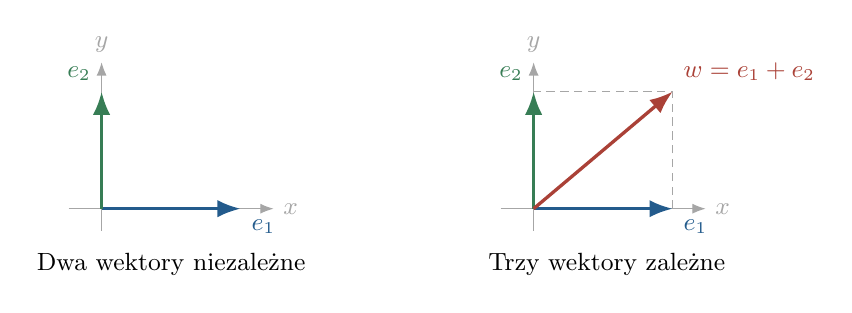
\begin{tikzpicture}[>=Latex,scale=0.93,every node/.style={font=\small}]
 \begin{scope}
  \draw[->,gray!70] (-0.45,0)--(2.35,0) node[right] {\(x\)};
  \draw[->,gray!70] (0,-0.3)--(0,2.0) node[above] {\(y\)};
  \draw[->,very thick,manifoldblue] (0,0)--(1.9,0)
       node[below right] {\(e_1\)};
  \draw[->,very thick,manifoldgreen] (0,0)--(0,1.6)
       node[above left] {\(e_2\)};
  \node at (0.95,-0.76) {Dwa wektory niezależne};
 \end{scope}
 \begin{scope}[xshift=5.9cm]
  \draw[->,gray!70] (-0.45,0)--(2.35,0) node[right] {\(x\)};
  \draw[->,gray!70] (0,-0.3)--(0,2.0) node[above] {\(y\)};
  \draw[densely dashed,gray!70] (1.9,0)--(1.9,1.6)--(0,1.6);
  \draw[->,very thick,manifoldblue] (0,0)--(1.9,0)
       node[below right] {\(e_1\)};
  \draw[->,very thick,manifoldgreen] (0,0)--(0,1.6)
       node[above left] {\(e_2\)};
  \draw[->,very thick,manifoldred] (0,0)--(1.9,1.6)
       node[above right] {\(w=e_1+e_2\)};
  \node at (1.0,-0.76) {Trzy wektory zależne};
 \end{scope}
\end{tikzpicture}
\caption{Niezależność nie oznacza jedynie niezerowości wektorów.
Dwa wektory \(e_1,e_2\) są niezależne, lecz po dołączeniu
\(w=e_1+e_2\) otrzymujemy rodzinę zależną.
Linie przerywane ilustrują dodawanie wektorów.}
\label{fig:lin-niezaleznosc-r2}
\end{figure}

\begin{przyklad}[Charakterystyka dwa]
\label{prz:lin-f2}
W \(\mathbb F_2^2\) występują trzy niezerowe wektory:
\(u=(1,0)\), \(v=(0,1)\), \(w=(1,1)\).
Każde dwa różne wektory niezerowe są niezależne.
Istotnie, jeśli dla takich wektorów \(a,b\)
mamy \(\alpha a+\beta b=0\) z
\(\alpha,\beta\in\mathbb F_2\), to tylko
współczynniki \(0\) i \(1\) są możliwe.
Przypadki \((\alpha,\beta)=(1,0)\)
oraz \((0,1)\) przeczą niezerowości
wektorów. Przypadek \((1,1)\)
dawałby \(a+b=0\), a więc \(a=b\)
w charakterystyce \(2\), również sprzeczność.
Stąd \(\alpha=\beta=0\).
Jednak wszystkie trzy wektory są zależne, ponieważ
\(u+v+w=(0,0)\) nad \(\mathbb F_2\).
W \(\mathbb F_2^2\) nie można więc opisywać
niezależności za pomocą kątów ani długości.
\end{przyklad}

\section{Bazy i wymiar w przypadku skończonym}
\label{sec:lin-bazy-skonczone}

\begin{definicja}[Baza i wymiar]
\label{def:lin-baza}
\emph{Bazą} przestrzeni \(V\) nazywamy rodzinę
wektorów, która jest liniowo niezależna i rozpina \(V\).
Przestrzeń nazywamy \emph{skończenie wymiarową},
jeżeli posiada skończoną bazę.
W szczególności pusta rodzina jest bazą przestrzeni \(\{0\}\).
Jeżeli \(V\) ma skończoną bazę składającą się z \(n\)
wektorów, to liczbę \(n\) nazywamy jej \emph{wymiarem}
i oznaczamy \(\dim_KV=n\).
Wykażemy niżej, że liczba ta nie zależy od wybranej bazy.
\end{definicja}

Baza łączy dwa warunki, które oddzielnie nie wystarczają:
generatory mogą zawierać powtórzenia i nadmiarowe wektory,
natomiast rodzina niezależna może nie rozpinać całej przestrzeni.

\begin{lemat}[Usuwanie zbędnych generatorów]
\label{lem:lin-usuwanie-generatorow}
Jeżeli skończona rodzina \((s_1,\ldots,s_m)\)
rozpina \(V\), to można usunąć z niej pewne
wektory, otrzymując bazę \(V\).
\end{lemat}
\begin{proof}
Jeśli rodzina jest niezależna, jest już bazą.
W przeciwnym razie istnieją skalary
\(a_1,\ldots,a_m\), nie wszystkie zerowe, takie że
\(\sum_{j=1}^m a_js_j=0\).
Wybieramy \(k\) z \(a_k\neq0\). Wówczas
\(s_k=-a_k^{-1}\sum_{j\neq k}a_js_j\).
Każde wystąpienie \(s_k\) w kombinacji generatorów
można zastąpić tą sumą, więc rodzina bez \(s_k\)
nadal rozpina \(V\). Powtarzamy procedurę.
Liczba wektorów za każdym razem maleje, toteż
po co najwyżej \(m\) krokach otrzymamy rodzinę
niezależną. Przypadek \(V=\{0\}\) kończy się
rodziną pustą, która nadal rozpina \(V\).
\end{proof}

\begin{twierdzenie}[Lemat o wymianie Steinitza]
\label{thm:lin-steinitz}
Niech \(V\) będzie przestrzenią wektorową nad \(K\).
Załóżmy, że \(V\) rozpina skończona rodzina
\((s_1,\ldots,s_m)\) i że
\((v_1,\ldots,v_r)\) jest rodziną liniowo niezależną.
Wtedy \(r\leq m\). Co więcej, można wybrać
\(r\) pozycji w rodzinie \((s_1,\ldots,s_m)\)
i zastąpić znajdujące się w nich wektory kolejno
przez \(v_1,\ldots,v_r\), tak by powstała
\(m\)-elementowa rodzina rozpinająca \(V\).
Nie zakładamy, że początkowa rodzina generatorów
jest niezależna.
\end{twierdzenie}
\begin{proof}
Najpierw, dla \(0\leq k\leq\min\{m,r\}\),
konstruujemy indukcyjnie rodzinę rozpinającą, złożoną
z \(v_1,\ldots,v_k\) oraz \(m-k\)
wektorów pozostawionych z wyjściowej rodziny.
Przy \(k=0\) jest to założenie.

Załóżmy, że zbudowaliśmy taką rodzinę
dla \(k<\min\{m,r\}\).
Ponieważ rozpina ona \(V\), wektor \(v_{k+1}\)
ma przedstawienie
\(v_{k+1}=\sum_{i=1}^{k}a_iv_i+
                 \sum_{j\in J_k}b_js_j\),
gdzie \(J_k\) jest zbiorem \(m-k\)
pozostałych pozycji generatorów.
Co najmniej jeden z \(b_j\) jest niezerowy.
Gdyby wszystkie były zerowe, wektor \(v_{k+1}\)
należałby do przestrzeni rozpiętej przez
\(v_1,\ldots,v_k\), co przeczy niezależności
rodziny \(v_1,\ldots,v_r\).

Wybieramy więc \(j_0\in J_k\) z
\(b_{j_0}\neq0\) i rozwiązujemy tę równość
względem \(s_{j_0}\):
\[
 s_{j_0}=b_{j_0}^{-1}v_{k+1}
   -\sum_{i=1}^{k}b_{j_0}^{-1}a_iv_i
   -\sum_{j\in J_k\setminus\{j_0\}}
                       b_{j_0}^{-1}b_js_j .
\]
Zatem nowa rodzina, w której \(s_{j_0}\)
zastąpiono \(v_{k+1}\), rozpina wszystkie
wektory poprzedniej rodziny, a więc całe \(V\).
Ma \(k+1\) wektorów z rodziny \(v_i\)
i \(m-k-1\) pozostałych generatorów.
Zachowujemy tezę indukcyjną.

Jeżeli \(r>m\), to po \(m\) krokach
otrzymujemy rodzinę \((v_1,\ldots,v_m)\)
rozpinającą \(V\), ponieważ wykorzystaliśmy
wszystkie \(m\) pozycji generatorów.
Wówczas \(v_{m+1}\) również należałby
do \(\operatorname{span}\{v_1,\ldots,v_m\}\),
wbrew niezależności rodziny \((v_1,\ldots,v_r)\).
Zatem \(r\leq m\). Indukcję można więc
przeprowadzić do kroku \(r\), otrzymując
zapowiedzianą rodzinę rozpinającą.
\end{proof}

\begin{wniosek}[Jednakowa liczba elementów baz skończonych]
\label{cor:lin-bazy-rowna-liczba}
Jeżeli \(B=(b_1,\ldots,b_n)\) i
\(C=(c_1,\ldots,c_m)\) są skończonymi bazami
tej samej przestrzeni \(V\), to \(n=m\).
\end{wniosek}
\begin{proof}
Rodzina \(B\) jest niezależna, a \(C\) rozpina \(V\),
więc z Twierdzenia~\ref{thm:lin-steinitz}
wynika \(n\leq m\).
Zamieniając role \(B\) i \(C\), dostajemy \(m\leq n\).
Stąd \(n=m\), co uzasadnia jednoznaczność
wymiaru z Definicji~\ref{def:lin-baza}.
\end{proof}

\begin{twierdzenie}[Uzupełnianie rodziny niezależnej do bazy]
\label{thm:lin-uzupelnianie-skonczone}
Niech \(V\) będzie rozpięta przez skończoną rodzinę
\((s_1,\ldots,s_m)\), a
\((v_1,\ldots,v_r)\) niech będzie rodziną
liniowo niezależną w \(V\).
Wówczas pewne wektory spośród \(s_1,\ldots,s_m\)
można dołączyć do \((v_1,\ldots,v_r)\)
tak, aby otrzymać bazę \(V\).
\end{twierdzenie}
\begin{proof}
Rozważamy skończoną rodzinę
\((v_1,\ldots,v_r,s_1,\ldots,s_m)\).
Przechodzimy kolejno przez elementy
\(s_1,\ldots,s_m\). Wektor \(s_j\) dołączamy
do dotychczas wybranej rodziny dokładnie wtedy,
gdy nie leży w jej przestrzeni rozpiętej.
Ponieważ dołączamy \(s_j\) tylko wtedy, gdy
nie należy do przestrzeni rozpiętej przez już
wybrane wektory, nie jest on w szczególności
powtórzeniem żadnego z nich.
Z Wniosku~\ref{cor:lin-podrodziny}
wynika więc, że po każdym kroku
zachowujemy liniową niezależność.
Jeśli wektor pominięto, był już kombinacją
wektorów dotychczas wybranych, więc także
końcowych. Jeśli dołączono, również należy
do ich przestrzeni rozpiętej.
Po ostatnim kroku wszystkie \(s_j\)
leżą więc w przestrzeni rozpiętej przez wybraną
rodzinę. Skoro \(s_j\) rozpinają \(V\), wybrana
rodzina też rozpina \(V\), a zatem jest bazą.
\end{proof}

\begin{wniosek}[Kryteria bycia bazą]
\label{cor:lin-baza-kryteria}
Niech \(V\) ma wymiar \(n<\infty\).
Wtedy:
\begin{enumerate}[label=(\roman*)]
\item każda rodzina niezależna ma co najwyżej \(n\) wektorów;
\item każda skończona rodzina rozpinająca ma co najmniej \(n\) wektorów;
\item rodzina złożona z dokładnie \(n\) wektorów jest bazą,
      jeżeli jest niezależna \emph{albo} rozpina \(V\).
\end{enumerate}
\end{wniosek}
\begin{proof}
W punkcie (i) stosujemy Twierdzenie~\ref{thm:lin-steinitz}
do dowolnej niezależnej rodziny i ustalonej bazy
\(n\)-elementowej. Gdyby niezależna rodzina
miała więcej niż \(n\) elementów, jej podrodzina
z \(n+1\) elementami przeczyłaby temu twierdzeniu.
Punkt (ii) otrzymujemy, stosując to samo twierdzenie
do ustalonej bazy niezależnej i rodziny rozpinającej.

Jeżeli rodzina \(n\)-elementowa jest niezależna,
uzupełniamy ją do bazy z
Twierdzenia~\ref{thm:lin-uzupelnianie-skonczone}.
Nowa baza musi mieć \(n\) elementów,
więc nic nie można było dołączyć;
rodzina wyjściowa już rozpina \(V\).
Jeżeli rodzina \(n\)-elementowa rozpina \(V\),
usuwamy z niej zależne elementy
zgodnie z Lematem~\ref{lem:lin-usuwanie-generatorow}.
Powstała baza ma \(n\) elementów,
więc żaden element nie został usunięty.
\end{proof}

\begin{twierdzenie}[Wymiar podprzestrzeni]
\label{thm:lin-wymiar-podprzestrzeni}
Niech \(V\) będzie przestrzenią skończenie wymiarową
nad \(K\), a \(W\subseteq V\) jej podprzestrzenią.
Wtedy \(W\) jest skończenie wymiarowa oraz
\(\dim_KW\leq\dim_KV\).
Ponadto równość wymiarów zachodzi dokładnie wtedy,
gdy \(W=V\).
\end{twierdzenie}
\begin{proof}
Oznaczmy \(n=\dim_KV\). Jeśli \(W=\{0\}\),
to pusta rodzina jest bazą \(W\), a więc
\(\dim_KW=0\leq n\).
Załóżmy, że \(W\neq\{0\}\).
Wybierzmy \(w_1\in W\setminus\{0\}\).
Rodzina \((w_1)\) jest niezależna.
Jeśli \(\operatorname{span}\{w_1\}\neq W\),
wybieramy \(w_2\in W\setminus\operatorname{span}\{w_1\}\).
Z Wniosku~\ref{cor:lin-podrodziny} wynika,
że \((w_1,w_2)\) jest niezależna.
Postępujemy tak dalej: jeżeli wybrane wektory
nie rozpinają \(W\), dołączamy jeden z \(W\)
spoza ich przestrzeni rozpiętej.
Każdy krok powiększa niezależną rodzinę.
Ponieważ taka rodzina w \(V\) ma co najwyżej
\(n\) elementów (Wniosek~\ref{cor:lin-baza-kryteria}),
procedura musi zakończyć się po skończenie wielu krokach.
Otrzymujemy bazę \(W\) liczącą \(r\leq n\) wektorów.

Jeżeli \(W=V\), równość wymiarów jest oczywista.
Odwrotnie, jeśli \(r=n\), otrzymana baza
\(W\) jest niezależną rodziną \(n\) wektorów w \(V\).
Z Wniosku~\ref{cor:lin-baza-kryteria}(iii)
rozpina ona także \(V\). Wszystkie jej
wektory należą do \(W\), więc \(V\subseteq W\),
a stąd \(V=W\).
\end{proof}

\begin{przyklad}[Bazy kanoniczne przestrzeni współrzędnych i macierzy]
\label{prz:lin-bazy-macierzy}
Niech \(n\geq1\). Dla \(j\in\{1,\ldots,n\}\)
oznaczmy przez \(e_j\in K^n\) wektor,
którego \(j\)-ta współrzędna wynosi \(1_K\),
a pozostałe \(0_K\). Każdy \(x=(x_1,\ldots,x_n)\)
ma zapis \(x=\sum_{j=1}^n x_je_j\);
jeżeli \(\sum_{j=1}^n a_je_j=0\),
to porównanie \(j\)-tej współrzędnej daje \(a_j=0\).
Zatem \((e_1,\ldots,e_n)\) jest bazą \(K^n\)
i \(\dim_K K^n=n\). Dla \(n=0\) odpowiednie
stwierdzenie pozostaje prawdziwe z bazą pustą.

Dla \(m,n\geq1\) niech
\(\operatorname{Mat}_{m\times n}(K)\) oznacza
przestrzeń wszystkich macierzy o \(m\) wierszach
i \(n\) kolumnach, z dodawaniem i mnożeniem
przez skalar wykonywanymi po elementach.
Niech \(E_{ij}\) będzie macierzą, której
wyraz na pozycji \((i,j)\) wynosi \(1_K\),
a pozostałe \(0_K\).
Każda macierz \(A=(a_{ij})\) ma zapis
\(A=\sum_{i=1}^m\sum_{j=1}^n a_{ij}E_{ij}\).
Jeśli ta suma jest macierzą zerową,
porównanie jej wyrazu \((i,j)\) daje \(a_{ij}=0\).
Macierze \(E_{ij}\) tworzą zatem bazę
i \(\dim_K\operatorname{Mat}_{m\times n}(K)=mn\).
\end{przyklad}

\begin{uwaga}[Definicja wymiaru a liczność rodziny]
\label{rem:lin-dim-nie-baza}
Dla przestrzeni \(\{0\}\) wymiar wynosi \(0\),
ponieważ pusta rodzina jest bazą. Nie istnieje
jednoelementowa baza przestrzeni zerowej:
jej jedyny wektor \(0\) jest liniowo zależny.
Nie wolno również wnioskować o wymiarze
wyłącznie z liczby podanych generatorów
bez zbadania ich niezależności.
\end{uwaga}

\section{Współrzędne względem bazy}
\label{sec:lin-wspolrzedne}

\begin{twierdzenie}[Jednoznaczność współrzędnych]
\label{thm:lin-wspolrzedne}
Niech \(V\) będzie \(n\)-wymiarową przestrzenią
nad \(K\), a \(B=(b_1,\ldots,b_n)\) jej bazą.
Dla każdego \(v\in V\) istnieje dokładnie jedna
kolumna \((a_1,\ldots,a_n)\in K^n\) taka, że
\(v=\sum_{i=1}^n a_ib_i\).
Odwzorowanie
\[
 [\,\cdot\,]_B\colon V\longrightarrow K^n,\qquad
 v\longmapsto(a_1,\ldots,a_n)
\]
jest bijekcją oraz zachowuje dodawanie
i mnożenie przez skalary.
\end{twierdzenie}
\begin{proof}
Istnienie zapisu wynika z faktu, że baza rozpina \(V\),
a jednoznaczność z
Lematu~\ref{lem:lin-niezaleznosc-kryteria}.
Jeśli \(v=\sum a_ib_i\) i \(w=\sum c_ib_i\),
to z rozdzielności działań wynika
\(v+w=\sum(a_i+c_i)b_i\) i
\(\lambda v=\sum(\lambda a_i)b_i\).
Jednoznaczność współczynników daje
\([v+w]_B=[v]_B+[w]_B\) oraz
\([\lambda v]_B=\lambda[v]_B\).
Dla dowolnej kolumny \((a_1,\ldots,a_n)\in K^n\)
wektor \(\sum a_ib_i\) ma dokładnie tę kolumnę
współrzędnych, więc odwzorowanie jest surjektywne.
Jeśli \([v]_B=[w]_B\), obie sumy są identyczne,
stąd \(v=w\), co dowodzi iniektywności.
\end{proof}

\begin{przyklad}[Współrzędne w niestandardowej bazie]
\label{prz:lin-wspolrzedne-niekanoniczne}
W \(\mathbb R^3\) rozważmy wektory
\(b_1=(1,1,0)\), \(b_2=(0,1,1)\),
\(b_3=(0,0,1)\).
Szukając współczynników \(a,b,c\) z
\((x,y,z)=ab_1+bb_2+cb_3\),
porównujemy współrzędne i otrzymujemy
\(x=a,\ y=a+b,\ z=b+c\).
Stąd jedyne możliwe rozwiązanie to
\(a=x\), \(b=y-x\), \(c=z-y+x\).
Jest ono poprawne dla każdego \((x,y,z)\in\mathbb R^3\),
a zatem rodzina \((b_1,b_2,b_3)\) jest bazą.
Na przykład
\([(2,3,5)]_B=(2,1,4)\), ponieważ
\(2b_1+b_2+4b_3=(2,3,5)\).
\end{przyklad}

\begin{przyklad}[Baza wielomianów]
\label{prz:lin-baza-wielomianow}
W \(K[X]_{\leq d}\) wektory \(1,X,\ldots,X^d\)
rozpinają przestrzeń z definicji wielomianu.
Równość \(\sum_{j=0}^d a_jX^j=0\)
jest równością wielomianów, a więc wszystkie
współczynniki \(a_j\) są zerowe.
Wektory są niezależne i stanowią bazę,
zatem \(\dim_KK[X]_{\leq d}=d+1\).
Dla \(p(X)=2-3X+X^3\) nad \(\mathbb R\)
w bazie \((1,X,X^2,X^3)\) mamy
\([p]_B=(2,-3,0,1)\).
\end{przyklad}

\begin{przyklad}[Współrzędne zależą od ciała]
\label{prz:lin-wspolrzedne-ciala}
Dla \(z=2+3i\in\mathbb C\)
w bazie \(B=(1,i)\) przestrzeni nad
\(\mathbb R\) mamy \([z]_B=(2,3)\).
W bazie \((1)\) przestrzeni \(\mathbb C\)
nad \(\mathbb C\) współrzędną jest jednoelementowa
kolumna \((2+3i)\).
Są to opisy tego samego elementu w dwóch różnych
przestrzeniach wektorowych (nad różnymi ciałami).
\end{przyklad}

\section{Bazy algebraiczne w dowolnym wymiarze}
\label{sec:lin-bazy-nieskonczone}

Definicje przestrzeni rozpiętej, niezależności i bazy
nie wymagają skończoności wymiaru.
W nieskończonej bazie \((b_i)_{i\in I}\)
każdy wektor ma \emph{skończony} zapis
\(\sum_{i\in F}a_ib_i\) z \(F\subseteq I\) skończonym.
Taką bazę nazywamy \emph{bazą Hamela}.
Nie należy jej mylić z bazą Schauderowską,
w której dopuszcza się granice nieskończonych sum;
to drugie pojęcie wymaga topologii i należy do analizy funkcjonalnej.

\begin{przyklad}[Baza kanoniczna ciągów o skończonym nośniku]
\label{prz:lin-baza-skonczony-nosnik}
Dla \(n\in\mathbb N_0\) niech \(e_n\) oznacza ciąg,
którego \(n\)-ty wyraz jest równy \(1_K\),
a pozostałe są zerowe.
Rodzina \((e_n)_{n\in\mathbb N_0}\)
jest niezależna: w równości
\(\sum_{n\in F}a_ne_n=0\) odczytanie współrzędnej
o indeksie \(n\in F\) daje \(a_n=0\).
Rozpina \(K^{(\mathbb N_0)}\), bo każdy ciąg
o skończonym nośniku \(F\) ma postać
\(\sum_{n\in F}x_ne_n\).

Ta sama rodzina \emph{nie} rozpina
\(K^{\mathbb N_0}\): każda skończona kombinacja
wektorów \(e_n\) ma skończony nośnik, natomiast
ciąg \((1,1,\ldots)\) ma nośnik nieskończony.
Formalny napis \(\sum_{n=0}^{\infty}e_n\)
nie jest kombinacją liniową w sensie
Definicji~\ref{def:lin-span}.
\end{przyklad}

\begin{przyklad}[Baza wszystkich wielomianów]
\label{prz:lin-baza-kx}
Rodzina \((1,X,X^2,\ldots)\) jest bazą Hamela \(K[X]\).
Każdy wielomian zawiera skończenie wiele potęg \(X\)
i jego zapis przez te potęgi jest jednoznaczny.
Przestrzeń \(K[X]\) nie ma skończonej bazy:
jeśli rozpinają ją \(p_1,\ldots,p_m\),
to przy istnieniu choć jednego niezerowego
generatora każda niezerowa ich kombinacja
ma stopień nie większy niż
\(d=\max\{\deg p_j:p_j\neq0\}\).
Zbiór, którego maksimum bierzemy, jest
wtedy niepusty i skończony.
Wtedy \(X^{d+1}\) nie należy do ich przestrzeni
rozpiętej. Jeśli wszystkie \(p_j\) są zerowe
(lub \(m=0\)), nie rozpinają nawet wielomianu \(1\).
\end{przyklad}

\begin{lemat}[Łańcuch rodzin niezależnych]
\label{lem:lin-lancuchy}
Niech \(\mathcal C\) będzie rodziną liniowo
uporządkowaną przez zawieranie,
której elementy są liniowo niezależnymi
podzbiorami \(V\).
Wtedy \(\bigcup_{S\in\mathcal C}S\)
jest liniowo niezależny.
\end{lemat}
\begin{proof}
W każdej ewentualnej relacji liniowej występuje
tylko skończenie wiele wektorów \(v_1,\ldots,v_m\).
Każdy należy do pewnego zbioru \(S_j\in\mathcal C\).
Ponieważ \(\mathcal C\) jest łańcuchem, spośród
skończonej rodziny \(S_1,\ldots,S_m\)
można wybrać zbiór największy względem zawierania.
Zawiera on wszystkie \(v_j\), a jest niezależny.
Stąd współczynniki relacji są zerowe.
Dla pustego łańcucha unia jest zbiorem pustym,
również niezależnym.
\end{proof}

\begin{twierdzenie}[Istnienie bazy i rozszerzanie rodziny niezależnej]
\label{thm:lin-istnienie-bazy-zorn}
Przyjmijmy aksjomat wyboru (równoważnie: lemat Zorna).
Dla każdej przestrzeni wektorowej \(V\) nad \(K\)
i każdego liniowo niezależnego zbioru
\(S_0\subseteq V\) istnieje baza Hamela \(B\)
taka, że \(S_0\subseteq B\).
W szczególności każda przestrzeń wektorowa ma bazę.
\end{twierdzenie}
\begin{proof}
Niech \(\mathcal P\) będzie rodziną wszystkich
liniowo niezależnych podzbiorów \(V\)
zawierających \(S_0\), uporządkowaną
przez zawieranie. Rodzina jest niepusta,
bo \(S_0\in\mathcal P\).
Niech \(\mathcal C\subseteq\mathcal P\)
będzie dowolnym łańcuchem.
Jeżeli \(\mathcal C=\varnothing\),
ograniczeniem górnym w \(\mathcal P\)
jest \(S_0\).
Jeżeli \(\mathcal C\neq\varnothing\),
jego unia \(\bigcup_{S\in\mathcal C}S\)
zawiera \(S_0\), ponieważ każdy
\(S\in\mathcal C\) zawiera \(S_0\).
Unia jest niezależna na mocy
Lematu~\ref{lem:lin-lancuchy},
więc należy do \(\mathcal P\)
i stanowi ograniczenie górne łańcucha.

Lemat Zorna zapewnia istnienie maksymalnego
elementu \(B\in\mathcal P\).
Przypuśćmy, że \(\operatorname{span}(B)\neq V\)
i wybierzmy \(v\in V\setminus\operatorname{span}(B)\).
Dowód Wniosku~\ref{cor:lin-podrodziny}
pokazuje, że \(B\cup\{v\}\) jest niezależny.
Zawiera ściśle \(B\) i nadal należy do
\(\mathcal P\), w sprzeczności z maksymalnością.
Zatem \(\operatorname{span}(B)=V\),
co oznacza, że \(B\) jest bazą.
\end{proof}

\begin{uwaga}[Zakres użycia aksjomatu wyboru]
\label{rem:lin-aksjomat-wyboru}
Dowód istnienia bazy dla przestrzeni skończenie
generowanych nie wymaga lematu Zorna:
wystarcza procedura z
Lematu~\ref{lem:lin-usuwanie-generatorow}.
Dla ogólnej przestrzeni nieskończenie wymiarowej
w powyższym dowodzie zastosowaliśmy aksjomat wyboru.
Bez dodatkowych założeń teoriomnogościowych nie
można w ZF dowieść ogólnego twierdzenia,
że każda przestrzeń wektorowa ma bazę.
Jednoznaczność mocy dwóch baz nieskończonych
będzie tematem następnego rozdziału,
gdzie omówimy wymiar jako liczbę kardynalną.
\end{uwaga}

\begin{twierdzenie}[Charakteryzacje bazy]
\label{thm:lin-charakterystyki-bazy}
Dla dowolnego podzbioru \(B\subseteq V\)
następujące warunki są równoważne:
\begin{enumerate}[label=(\roman*)]
\item \(B\) jest bazą \(V\);
\item \(B\) jest maksymalnym względem zawierania
      liniowo niezależnym podzbiorem \(V\);
\item \(B\) jest minimalnym względem zawierania
      zbiorem rozpinającym \(V\).
\end{enumerate}
\end{twierdzenie}
\begin{proof}
Jeśli \(B\) jest bazą, to żaden wektor spoza \(B\)
nie może zostać dołączony bez powstania zależności,
bo każdy wektor należy do \(\operatorname{span}(B)\).
Zatem baza jest maksymalnie niezależna.
Jeśli \(B\) jest maksymalnie niezależny, a nie rozpina \(V\),
można dobrać \(v\notin\operatorname{span}(B)\)
i powiększyć \(B\) do niezależnego zbioru,
wbrew maksymalności. Daje to (ii)\(\Rightarrow\)(i).

Jeśli \(B\) jest bazą, usunięcie któregokolwiek
\(b\in B\) uniemożliwia rozpięcie \(b\)
przez pozostałe elementy na mocy
Lematu~\ref{lem:lin-niezaleznosc-kryteria}.
Istotnie, gdyby właściwy podzbiór \(C\subsetneq B\)
rozpinał \(V\), to po wybraniu
\(b\in B\setminus C\) również
\(B\setminus\{b\}\supseteq C\) rozpinałby \(V\),
wbrew poprzedniemu wnioskowi.
Zatem baza jest minimalnym zbiorem rozpinającym,
co daje (iii).
Jeśli zbiór \(B\) rozpina \(V\), ale jest zależny,
to dla pewnego \(b\in B\) zachodzi
\(b\in\operatorname{span}(B\setminus\{b\})\).
Po usunięciu \(b\) nadal rozpinamy \(V\),
wbrew minimalności. Otrzymujemy (iii)\(\Rightarrow\)(i).
\end{proof}

\section{Zastosowanie: podprzestrzeń zadana rekurencją}
\label{sec:lin-przyklad-rekurencja}

\begin{przyklad}[Ciągi Fibonacciego z dowolnymi danymi początkowymi]
\label{prz:lin-rekurencja}
Niech \(V=\mathbb R^{\mathbb N_0}\).
Rozważmy zbiór
\[
 W=\{x=(x_n)_{n\geq0}\in V:
                   x_{n+2}=x_{n+1}+x_n
                   \text{ dla każdego }n\geq0\}.
\]
Jest on podprzestrzenią: ciąg zerowy spełnia
rekurencję, a jeśli \(x,y\) ją spełniają,
to dla \(a,b\in\mathbb R\)
\[
 (ax+by)_{n+2}
 =a(x_{n+1}+x_n)+b(y_{n+1}+y_n)
 =(ax+by)_{n+1}+(ax+by)_n .
\]
Zadanie dwóch pierwszych wyrazów
\(x_0=s,\ x_1=t\) wyznacza dokładnie
jeden ciąg z \(W\): następne wyrazy
obliczamy kolejno z rekurencji.
Niech \(u\in W\) ma dane początkowe
\((1,0)\), a \(v\in W\) dane \((0,1)\).
Wtedy każdy \(x\in W\) ma postać
\(x=x_0u+x_1v\): obie strony mają te
same dane początkowe i spełniają
tę samą rekurencję, więc są równe
na mocy indukcji po indeksie \(n\).
Jeśli \(au+bv=0\), porównanie wyrazów
o indeksach \(0,1\) daje \(a=b=0\).
Zatem \((u,v)\) jest bazą \(W\)
i \(\dim_{\mathbb R}W=2\).

Ważny wniosek: \(W\) jest przestrzenią
dwuwymiarową, choć jej wektory są
\emph{nieskończonymi} ciągami.
Liczba współrzędnych używanych do
opisania elementu nie jest sama
w sobie wymiarem przestrzeni.
\end{przyklad}

\section{Podsumowanie zależności logicznych}
\label{sec:lin-podsumowanie}

W rozdziale nie utożsamialiśmy przestrzeni
wektorowej z \(K^n\): istnienie współrzędnych
wynika dopiero z wyboru bazy.
W przypadku skończenie generowanym
udowodniliśmy bez aksjomatu wyboru:
istnienie bazy, lemat o wymianie,
równość liczby elementów baz oraz
jednoznaczność współrzędnych.
Dla dowolnych przestrzeni
istnienie bazy uzyskaliśmy z lematu Zorna.
Dla ustalonego podzbioru \(B\subseteq V\)
otrzymaliśmy równoważne opisy bazy:
\(B\) jest liniowo niezależny i
\(\operatorname{span}(B)=V\) wtedy i tylko wtedy,
gdy każdy \(v\in V\) posiada dokładnie jedno
przedstawienie jako skończona kombinacja liniowa
elementów \(B\).
To ostatnie sformułowanie wymaga
\emph{obu} warunków: istnienia i jednoznaczności
przedstawienia.
W kolejnym rozdziale rozwiniemy pojęcie wymiaru,
sumy i ilorazy podprzestrzeni oraz
konstrukcje nieskończenie wymiarowe.

\chapter{Wymiar, sumy proste i przestrzenie ilorazowe}
\label{ch:lin2-wymiar-sumy-ilorazy}
\index{wymiar przestrzeni wektorowej@Wymiar przestrzeni wektorowej}
\index{suma prosta@Suma prosta}
\index{przestrzen ilorazowa@Przestrzeń ilorazowa}

\noindent\textbf{Cel rozdziału.}
W Rozdziale~\ref{ch:lin-przestrzenie-wektorowe} zdefiniowaliśmy przestrzenie
wektorowe, skonstruowaliśmy bazy i dowiedliśmy jednoznaczności współrzędnych.
Teraz zbadamy wymiar dowolnej przestrzeni, sumy podprzestrzeni, sumy proste,
przestrzenie ilorazowe oraz dopełnienia algebraiczne.
Jeżeli składnikami sumy są \emph{wektory}, zawsze dopuszczamy
wyłącznie skończenie wiele niezerowych składników, nawet gdy zbiór
indeksów jest nieskończony. Nie rozważamy granic ani zbieżności
szeregów. Natomiast wyrażenie \(\sum_{i\in I}\dim_KU_i\)
oznacza \emph{sumę kardynalną} liczb \(\dim_KU_i\);
nie jest ono sumą wektorów.

W całym rozdziale \(K\) jest ciałem przemiennym, \(0_K\neq1_K\),
a wszystkie przestrzenie wektorowe są rozpatrywane nad \(K\).
Przy twierdzeniach o dowolnych bazach nieskończonych
jawnie przyjmujemy aksjomat wyboru; twierdzenia dotyczące skończonych
wymiarów nie wymagają go.

\section{Wymiar jako liczba kardynalna}
\label{sec:lin2-wymiar-kardynalny}

Dla baz skończonych jednakową liczbę wektorów
udowodniliśmy w Rozdziale~\ref{ch:lin-przestrzenie-wektorowe}
za pomocą lematu o wymianie Steinitza.
W przypadku dowolnych baz Hamela konieczny jest dodatkowy argument:
każdy wektor korzysta tylko ze skończenie wielu współrzędnych
w danej bazie.

\begin{lemat}[Nośnik współrzędnych w bazie]
\label{lem:lin2-nosnik}
Niech \(B\subseteq V\) będzie bazą Hamela.
Każdy wektor \(v\in V\) ma dokładnie jedną rodzinę
współczynników \((a_b)_{b\in B}\) o skończonym nośniku
taką, że \(v=\sum_{b\in B}a_bb\).
Oznaczmy przez \(\operatorname{supp}_B(v)\) zbiór
tych \(b\in B\), dla których \(a_b\neq0_K\).
Dla dowolnego \(A\subseteq B\) zachodzi
\[
 \operatorname{span}(A)
 =\{v\in V:\operatorname{supp}_B(v)\subseteq A\}.
\]
\end{lemat}
\begin{proof}
Z Twierdzenia~\ref{thm:lin-wspolrzedne-hamela}
wynikają istnienie przedstawienia
oraz jednoznaczność rodziny współczynników.
Jeśli \(v\in\operatorname{span}(A)\), to jest skończoną
kombinacją wektorów z \(A\). Po dopisaniu zerowych współczynników
poza \(A\) otrzymujemy przedstawienie względem \(B\).
Jednoznaczność pokazuje, że nośnik jest podzbiorem \(A\).
W przeciwnym kierunku, jeśli nośnik współczynników
\(v\) jest zawarty w \(A\), to jego jedyny zapis
w bazie \(B\) jest skończoną kombinacją elementów \(A\).
Równość obejmuje też \(v=0_V\) oraz \(A=\varnothing\).
\end{proof}

\begin{lemat}[Suma zbiorów skończonych indeksowana zbiorem nieskończonym]
\label{lem:lin2-moce-nosnikow}
Przyjmijmy aksjomat wyboru.
Niech \(I\) będzie zbiorem nieskończonym,
a \((F_i)_{i\in I}\) rodziną zbiorów skończonych.
Wtedy
\[
 \left|\bigcup_{i\in I}F_i\right|\leq |I|.
\]
\end{lemat}
\begin{proof}
Przyjmując twierdzenie o dobrym uporządkowaniu,
ustalmy dobre uporządkowania \(I\) oraz
\(D=\bigcup_{i\in I}F_i\).
Dla \(x\in D\) niech \(i(x)\) oznacza najmniejszy indeks
taki, że \(x\in F_{i(x)}\).
Uporządkowanie \(D\) wyznacza porządek
w skończonym zbiorze \(F_{i(x)}\).
Niech \(k(x)\in\mathbb N_0\) będzie numerem \(x\)
w tym skończonym uporządkowanym zbiorze.
Odwzorowanie
\(x\mapsto(i(x),k(x))\)
jest iniekcją z \(D\) do \(I\times\mathbb N_0\):
dla ustalonego \(i\) różne elementy \(F_i\)
otrzymują różne numery.
Zatem \(|D|\leq|I\times\mathbb N_0|=|I|\),
gdzie ostatnia równość jest standardowym
twierdzeniem arytmetyki kardynalnej w ZFC
dla zbioru nieskończonego \(I\).
\end{proof}

\begin{twierdzenie}[Równoliczność dowolnych baz]
\label{thm:lin2-jednakowa-moc-baz}
Przyjmijmy aksjomat wyboru.
Jeśli \(B,C\subseteq V\) są bazami Hamela
tej samej przestrzeni wektorowej \(V\),
to \(|B|=|C|\).
\end{twierdzenie}
\begin{proof}
Jeśli \(B\) jest skończona, to
z lematu o wymianie Steinitza
(Twierdzenie~\ref{thm:lin-steinitz})
każda skończona niezależna podrodzina \(C\)
ma co najwyżej \(|B|\) elementów.
Gdyby \(C\) miała więcej elementów,
można by wybrać \(|B|+1\) różnych elementów,
otrzymując sprzeczność.
Zatem \(C\) jest skończona, a jej liczność
jest równa \(|B|\) na mocy
Wniosku~\ref{cor:lin-bazy-rowna-liczba}.
To samo rozumowanie dotyczy zamienionych baz.
Pozostaje więc przypadek, gdy obie bazy są nieskończone.

Dla \(c\in C\) niech
\(F_c=\operatorname{supp}_B(c)\), skończony zbiór.
Pokażemy, że \(B=\bigcup_{c\in C}F_c\).
Zbiór \(D=\bigcup_{c\in C}F_c\) zawiera
wszystkie wektory potrzebne do zapisania
każdego \(c\in C\).
Stąd
\(\operatorname{span}(C)\subseteq\operatorname{span}(D)\).
Ponieważ \(C\) jest bazą \(V\),
otrzymujemy \(\operatorname{span}(D)=V\).
Gdyby \(b\in B\setminus D\), to
\(\operatorname{supp}_B(b)=\{b\}\not\subseteq D\),
a więc \(b\notin\operatorname{span}(D)\)
na mocy Lematu~\ref{lem:lin2-nosnik}, sprzeczność.
Wykazaliśmy zatem \(B=D\).

Z Lematu~\ref{lem:lin2-moce-nosnikow} otrzymujemy
\(|B|\leq|C|\).
Zamieniając role baz, dostajemy \(|C|\leq|B|\).
Twierdzenie Cantora--Bernsteina daje \(|B|=|C|\).
\end{proof}

\begin{definicja}[Wymiar w dowolnym wymiarze]
\label{def:lin2-wymiar}
Zakładając aksjomat wyboru, przez
\(\dim_K V\) rozumiemy moc dowolnej bazy Hamela \(V\).
Ta liczba kardynalna nie zależy od bazy
na mocy Twierdzenia~\ref{thm:lin2-jednakowa-moc-baz}.
W szczególności \(\dim_K\{0_V\}=0\).
\end{definicja}

\begin{przyklad}[Wymiar wielomianów i ciągów]
\label{prz:lin2-przeliczalna-baza}
W przestrzeni \(K[X]\) rodzina
\((1,X,X^2,\ldots)\) jest bazą.
Także \(K^{(\mathbb N_0)}\), przestrzeń ciągów
o skończonym nośniku, ma bazę \((e_n)_{n\in\mathbb N_0}\).
Obie bazy są przeliczalnie nieskończone:
\(\dim_KK[X]=\dim_KK^{(\mathbb N_0)}=\aleph_0\).
Izomorfizm tych przestrzeni przyporządkowuje
wielomianowi ciąg jego współczynników.
Nie należy mylić przestrzeni \(K^{(\mathbb N_0)}\)
z przestrzenią wszystkich ciągów \(K^{\mathbb N_0}\):
np. \((1,1,\ldots)\) nie należy do pierwszej z nich.
\end{przyklad}

\begin{uwaga}[Rachunek wymiarów nieskończonych]
\label{rem:lin2-odejmowanie-kardynalne}
Dla skończonych wymiarów możemy odejmować liczby naturalne.
Dla liczb kardynalnych nieskończonych odejmowanie
nie jest jednoznacznie odwracalne:
na przykład \(\aleph_0+1=\aleph_0+2=\aleph_0\).
Dlatego w ogólnych wzorach wymiarowych
będziemy stosować przede wszystkim dodawanie.
\end{uwaga}

\section{Suma algebraiczna podprzestrzeni}
\label{sec:lin2-suma-algebraiczna}

\begin{definicja}[Suma podprzestrzeni]
\label{def:lin2-suma-podprzestrzeni}
Niech \((U_i)_{i\in I}\) będzie rodziną podprzestrzeni \(V\).
\emph{Sumą algebraiczną} tej rodziny nazywamy
\[
 \sum_{i\in I}U_i:=
 \left\{\sum_{i\in F}u_i:
 F\subseteq I\text{ skończony},\
 u_i\in U_i\text{ dla każdego }i\in F\right\}.
\]
Przy \(I=\varnothing\) przyjmujemy sumę pustą
równą \(\{0_V\}\).
Dla dwóch podprzestrzeni piszemy
\(U+W=\{u+w:u\in U,\ w\in W\}\).
Nie należy mylić sumy algebraicznej \(U+W\)
z \emph{sumą zbiorów} \(U\cup W\).
\end{definicja}

\begin{twierdzenie}[Najmniejsza podprzestrzeń zawierająca rodzinę]
\label{thm:lin2-suma-minimalna}
Dla każdej rodziny \((U_i)_{i\in I}\)
podprzestrzeni \(V\) zbiór
\(\sum_{i\in I}U_i\) jest podprzestrzenią
i zachodzi
\[
 \sum_{i\in I}U_i=
 \operatorname{span}\!\left(\bigcup_{i\in I}U_i\right).
\]
Jest to najmniejsza podprzestrzeń \(V\)
zawierająca wszystkie \(U_i\).
\end{twierdzenie}
\begin{proof}
Suma zawiera \(0_V\), bo dopuszczamy sumę pustą.
Niech \(x=\sum_{i\in F}u_i\),
\(y=\sum_{i\in G}w_i\), gdzie \(F,G\subseteq I\)
są skończone, \(u_i\in U_i\), \(w_i\in U_i\).
Dopiszmy wektory zerowe przy brakujących indeksach,
dzięki czemu dla \(a,b\in K\)
\[
 ax+by=\sum_{i\in F\cup G}(au_i+bw_i).
\]
Każdy składnik należy do \(U_i\),
więc suma jest podprzestrzenią.

Każda \(U_i\) zawiera się w tej sumie:
wektor \(u\in U_i\) otrzymujemy z \(F=\{i\}\).
Zatem \(\operatorname{span}(\bigcup_iU_i)\)
jest zawarta w \(\sum_iU_i\).
W przeciwną stronę każdy składnik \(u_i\)
dowolnej sumy należy do \(\bigcup_iU_i\),
więc całe wyrażenie jest jej skończoną kombinacją.
Równość i minimalność wynikają z
Twierdzenia~\ref{thm:lin-span-minimalny}.
Przy \(I=\varnothing\) obie strony są
równe \(\{0_V\}\).
\end{proof}

\begin{stwierdzenie}[Rachunek sum podprzestrzeni]
\label{prop:lin2-rachunek-sum}
Dla podprzestrzeni \(U,W,Z\subseteq V\) zachodzą
\[
 U+W=W+U,\quad
 (U+W)+Z=U+(W+Z),\quad
 U+\{0_V\}=U,\quad U+U=U.
\]
Jeżeli \(U\subseteq W\), to \(U+Z\subseteq W+Z\).
Ponadto \(U\cap W\subseteq U+W\).
\end{stwierdzenie}
\begin{proof}
Pierwszą równość daje przemienność dodawania,
drugą łączność: obie strony składają się
dokładnie z wektorów \(u+w+z\).
Kolejne dwie równości wynikają
z obecności wektora zerowego i domknięcia
podprzestrzeni na dodawanie.
Zawieranie przy \(U\subseteq W\) jest bezpośrednie.
Dla \(v\in U\cap W\) mamy
\(v=v+0_V\in U+W\).
\end{proof}

\begin{przyklad}[Suma prostych na płaszczyźnie]
\label{prz:lin2-suma-prostych}
Niech \(U=\operatorname{span}\{(1,0)\}\),
\(W=\operatorname{span}\{(1,1)\}\subseteq\mathbb R^2\).
Dla każdego \((x,y)\in\mathbb R^2\)
otrzymujemy
\((x,y)=(x-y)(1,0)+y(1,1)\),
zatem \(U+W=\mathbb R^2\).
Jeśli \(a(1,0)=b(1,1)\), to
z drugiej współrzędnej \(b=0\),
a następnie \(a=0\).
Stąd \(U\cap W=\{0\}\).
Natomiast dla
\(Z=\operatorname{span}\{(2,0)\}\)
zachodzi \(U+Z=U\), chociaż
\(\dim U=\dim Z=1\).
\end{przyklad}

\begin{twierdzenie}[Wzór wymiarowy dla dwóch podprzestrzeni]
\label{thm:lin2-wzor-wymiarowy}
Przyjmijmy aksjomat wyboru.
Jeżeli \(U,W\) są podprzestrzeniami \(V\), to
\[
 \dim_K(U+W)+\dim_K(U\cap W)=\dim_KU+\dim_KW,
\]
gdzie dodawanie jest dodawaniem liczb kardynalnych.
Jeżeli \(U\) i \(W\) są skończenie wymiarowe, to
\[
 \dim_K(U+W)=\dim_KU+\dim_KW-\dim_K(U\cap W)
\]
jako równość liczb naturalnych, bez potrzeby
stosowania aksjomatu wyboru.
\end{twierdzenie}
\begin{proof}
Wybierzmy bazę \(C\) podprzestrzeni \(U\cap W\).
Rozszerzmy ją do bazy \(C\cup A\) przestrzeni \(U\)
oraz do bazy \(C\cup D\) przestrzeni \(W\).
Możemy przyjąć \(C\cap A=C\cap D=\varnothing\).
Ponadto \(A\cap D=\varnothing\):
każdy \(x\in A\cap D\) należałby do \(U\cap W\),
więc do \(\operatorname{span}(C)\),
co przeczyłoby niezależności \(C\cup A\).

Sprawdźmy, że \(C\cup A\cup D\) jest bazą \(U+W\).
Z definicji \(U+W\), każda jego składowa
\(u\in U\) jest kombinacją \(C\cup A\),
a każda \(w\in W\) jest kombinacją \(C\cup D\).
Wobec tego \(C\cup A\cup D\) rozpina \(U+W\).

Aby sprawdzić warunek niezależności liniowej,
przypuśćmy, że skończona kombinacja
elementów \(C\cup A\cup D\) jest równa zeru.
Po zebraniu składników otrzymujemy
\(c+a+d=0_V\), gdzie
\(c\in\operatorname{span}(C)\),
\(a\in\operatorname{span}(A)\),
\(d\in\operatorname{span}(D)\).
Ponieważ \(d=-(c+a)\in U\) oraz \(d\in W\),
mamy \(d\in U\cap W=\operatorname{span}(C)\).
Zapiszmy \(d\) raz jako skończoną kombinację
elementów \(D\), a drugi raz jako skończoną kombinację
elementów \(C\). Odejmując te dwa przedstawienia,
otrzymujemy równość z warunku niezależności liniowej
zbioru \(C\cup D\). Ponieważ \(C\cap D=\varnothing\),
wszystkie współczynniki w obu przedstawieniach
muszą być zerowe, a więc \(d=0_V\).
Następnie \(c+a=0_V\), a niezależność
\(C\cup A\) wymusza zerowanie również
pozostałych współczynników.
Wykazaliśmy niezależność całej rodziny.

Wobec tego, jako równości kardynalne,
\[
 \begin{aligned}
 \dim(U+W)&=|C|+|A|+|D|,&
 \dim(U\cap W)&=|C|,\\
 \dim U&=|C|+|A|,&
 \dim W&=|C|+|D|.
 \end{aligned}
\]
Po dodaniu stron otrzymujemy pierwszy wzór.
Dla wymiarów skończonych wolno odjąć
\(|C|=\dim(U\cap W)\) od obu stron,
co daje drugi wzór. W tym przypadku
bazy i ich rozszerzenia konstruujemy
skończonym algorytmem, bez aksjomatu wyboru.
\end{proof}

\begin{przyklad}[Płaszczyzny w \(\mathbb R^3\)]
\label{prz:lin2-plaszczyzny}
Niech \(U=\{(x,y,z):z=0\}\),
\(W=\{(x,y,z):y=0\}\subseteq\mathbb R^3\).
Przestrzenie te mają bazy \((e_1,e_2)\)
oraz \((e_1,e_3)\), więc wymiar \(2\).
Przecięcie to
\(U\cap W=\operatorname{span}\{e_1\}\)
o wymiarze \(1\).
Suma zawiera \(e_1,e_2,e_3\),
które rozpinają \(\mathbb R^3\),
więc \(U+W=\mathbb R^3\).
Wzór wymiarowy przyjmuje postać \(3+1=2+2\).
\end{przyklad}


\section{Sumy proste i jednoznaczność rozkładu}
\label{sec:lin2-sumy-proste}

\begin{definicja}[Wewnętrzna suma prosta]
\label{def:lin2-wewnetrzna-suma-prosta}
Niech \((U_i)_{i\in I}\) będzie rodziną
podprzestrzeni \(V\). Jej suma algebraiczna
jest \emph{sumą prostą}, jeśli dla każdego
skończonego \(F\subseteq I\) oraz
dowolnych \(u_i\in U_i\), \(i\in F\),
z równości
\[
 \sum_{i\in F}u_i=0_V
\]
wynika \(u_i=0_V\) dla wszystkich \(i\in F\).
Taką sumę oznaczamy przez
\(\bigoplus_{i\in I}U_i\).
Zapis \(V=\bigoplus_{i\in I}U_i\)
oznacza dodatkowo, że suma jest całą przestrzenią \(V\).
Dla \(I=\varnothing\) suma jest prosta
i jest równa \(\{0_V\}\).
\end{definicja}

\begin{twierdzenie}[Kryteria sumy prostej]
\label{thm:lin2-kryteria-sumy-prostej}
Dla dowolnej rodziny \((U_i)_{i\in I}\)
podprzestrzeni \(V\) następujące warunki są równoważne:
\begin{enumerate}[label=(\roman*)]
\item suma \(\sum_{i\in I}U_i\) jest prosta;
\item każdy wektor \(v\in\sum_{i\in I}U_i\)
ma dokładnie jedno przedstawienie
\(v=\sum_{i\in I}u_i\) z \(u_i\in U_i\)
i skończonym nośnikiem \(\{i:u_i\neq0_V\}\);
\item dla każdego \(j\in I\) zachodzi
\[
 U_j\cap\left(\sum_{i\in I\setminus\{j\}}U_i\right)
 =\{0_V\}.
\]
\end{enumerate}
Gdy \(I=\varnothing\), wszystkie trzy
warunki są spełnione.
Dla dwóch podprzestrzeni kryterium redukuje
się do \(U\cap W=\{0_V\}\).
\end{twierdzenie}
\begin{proof}
(i)\(\Rightarrow\)(ii): istnienie rozkładu
wynika z definicji sumy.
Jeśli \(v=\sum_i u_i=\sum_iw_i\)
dla dwóch rodzin o skończonych nośnikach,
to \(\sum_i(u_i-w_i)=0_V\).
Suma jest skończona, a warunek prostości
wymusza \(u_i-w_i=0_V\) dla wszystkich \(i\).
Stąd oba rozkłady są identyczne.

(ii)\(\Rightarrow\)(i): zerowy wektor
posiada rozkład o wszystkich składnikach zerowych.
Jeśli \(\sum_{i\in F}u_i=0_V\),
to otrzymujemy inny rozkład z wektorami \(u_i\),
rozszerzony zerami poza \(F\).
Jednoznaczność rozkładu oznacza,
że \(u_i=0_V\) dla każdego \(i\in F\).

(i)\(\Rightarrow\)(iii): weźmy
\(v\in U_j\cap\sum_{i\neq j}U_i\).
Istnieje skończony \(F\subseteq I\setminus\{j\}\)
oraz \(u_i\in U_i\) takie, że
\(v=\sum_{i\in F}u_i\).
Równość \(v-\sum_{i\in F}u_i=0_V\)
i prostość sumy dają \(v=0_V\).
W przeciwną stronę przyjmijmy (iii)
i niech \(\sum_{i\in F}u_i=0_V\).
Dla każdego \(j\in F\) mamy
\(u_j=-\sum_{i\in F\setminus\{j\}}u_i\).
Jest to element \(U_j\)
i sumy pozostałych podprzestrzeni,
zatem z (iii) otrzymujemy \(u_j=0_V\).
Dowodzi to (i).
Przy pustym \(I\) nie ma niezerowych składników
ani dodatkowych warunków do sprawdzenia.
\end{proof}

\begin{przyklad}[Zerowe przecięcia par nie wystarczają]
\label{prz:lin2-trzy-proste}
W \(\mathbb R^2\) rozważmy proste
\[
 U_1=\operatorname{span}\{(1,0)\},\qquad
 U_2=\operatorname{span}\{(0,1)\},\qquad
 U_3=\operatorname{span}\{(1,1)\}.
\]
Każde dwie z nich mają przecięcie \(\{0\}\):
żadne z różnych podanych wektorów
nie jest skalarną wielokrotnością drugiego.
Mimo to ich suma nie jest prosta, ponieważ
\((1,0)+(0,1)-(1,1)=(0,0)\),
a wszystkie trzy składniki są niezerowe.
W kryterium dla trzech i większej liczby
podprzestrzeni nie wystarczą więc
zerowe przecięcia par.
\end{przyklad}

\begin{definicja}[Zewnętrzna suma prosta]
\label{def:lin2-zewnetrzna-suma-prosta}
Dla rodziny \((U_i)_{i\in I}\)
przestrzeni wektorowych nad tym samym ciałem
definiujemy \emph{zewnętrzną sumę prostą}
\[
 \bigoplus_{i\in I}^{\mathrm{zew}}U_i
 :=\left\{(u_i)_{i\in I}\in\prod_{i\in I}U_i:
  \{i\in I:u_i\neq0_{U_i}\}\text{ jest skończony}\right\}.
\]
Dodawanie i mnożenie przez skalary
wykonujemy współrzędna po współrzędnej.
Dla \(I=\varnothing\) otrzymujemy
jednopunktową przestrzeń zerową.
\end{definicja}

\begin{twierdzenie}[Suma zewnętrzna a suma wewnętrzna]
\label{thm:lin2-zewn-wewn}
Jeżeli wszystkie \(U_i\) są podprzestrzeniami
jednej przestrzeni \(V\), to odwzorowanie
\[
 \Sigma\colon\bigoplus_{i\in I}^{\mathrm{zew}}U_i
 \longrightarrow\sum_{i\in I}U_i,\qquad
 (u_i)_{i\in I}\longmapsto\sum_{i\in I}u_i
\]
jest liniowe i surjektywne.
Jest izomorfizmem wtedy i tylko wtedy,
gdy suma podprzestrzeni jest prosta.
\end{twierdzenie}
\begin{proof}
Rodzina o skończonym nośniku ma dobrze określoną
skończoną sumę. Produkt \(\prod_{i\in I}U_i\)
jest przestrzenią wektorową z działaniami
współrzędnymi: każdy aksjomat wynika
z odpowiedniego aksjomatu w \(U_i\),
sprawdzonego dla każdego \(i\).
Przestrzeń zewnętrzna jest jego podprzestrzenią:
nośnik kombinacji \(a(u_i)+b(w_i)\)
zawiera się w sumie mnogościowej
dwóch skończonych zbiorów nośników.
Działania są zatem zamknięte.
Dla \(a,b\in K\) zachodzi
\(\Sigma(a(u_i)+b(w_i))
=a\Sigma((u_i))+b\Sigma((w_i))\);
oba rachunki obejmują tylko skończenie wiele indeksów.
Z definicji sumy algebraicznej każdy jej element
ma przedstawienie \(\sum_i u_i\),
więc \(\Sigma\) jest surjektywne.
Jest iniektywne dokładnie wtedy,
gdy \(\Sigma((u_i))=0_V\) wymusza
\(u_i=0_V\) dla wszystkich \(i\).
Jest to właśnie warunek prostości.
\end{proof}

\begin{twierdzenie}[Baza i wymiar sumy prostej]
\label{thm:lin2-wymiar-sumy-prostej}
Przyjmijmy aksjomat wyboru.
Niech \(V=\bigoplus_{i\in I}U_i\),
a \(B_i=(b_{i,j})_{j\in J_i}\)
niech będzie bazą Hamela \(U_i\).
Rodzina wszystkich \(b_{i,j}\)
z indeksami \((i,j)\), \(i\in I\), \(j\in J_i\),
jest bazą \(V\). Stąd
\[
 \dim_KV=\sum_{i\in I}\dim_KU_i
\]
jako równość liczb kardynalnych.
Jeśli bazy \(B_i\) są już wskazane,
część twierdzenia o bazie nie wymaga
dodatkowego zastosowania aksjomatu wyboru.
\end{twierdzenie}
\begin{proof}
Każdy \(v\in V\) jest skończoną sumą
\(u_i\in U_i\). Każdy z tych wektorów
jest skończoną kombinacją elementów \(B_i\).
Łącznie \(v\) jest skończoną kombinacją
elementów zestawionej rodziny,
która zatem rozpina \(V\).

Sprawdźmy warunek niezależności liniowej.
Jeśli skończona kombinacja elementów \(B_i\)
ze współczynnikami \(a_{i,j}\) daje zero,
zgrupujmy wyrazy według pierwszego indeksu:
\[
 \sum_{i\in F}
 \left(\sum_{j\in G_i}a_{i,j}b_{i,j}\right)=0_V.
\]
Prostość sumy podprzestrzeni daje,
że każde wyrażenie w nawiasie jest zerowe.
Niezależność rodziny \(B_i\) wymusza
\(a_{i,j}=0_K\) dla wszystkich \(i,j\).
Zestawiona rodzina jest zatem bazą.
Jej indeksy tworzą rozłączną sumę
zbiorów \(\{i\}\times J_i\);
liczba kardynalna elementów takiej sumy
jest z definicji sumą kardynalną liczb \(|J_i|\).
Otrzymujemy wzór.
\end{proof}

\begin{przyklad}[Rozkład wielomianów według parzystości potęg]
\label{prz:lin2-parzyste-nieparzyste}
Niech \(E\subseteq K[X]\) składa się
z wielomianów o niezerowych współczynnikach
wyłącznie przy parzystych potęgach,
a \(O\subseteq K[X]\) analogicznie
przy nieparzystych potęgach.
Obie przestrzenie zawierają wielomian zerowy.
Każdy wielomian \(p=\sum_{j=0}^d a_jX^j\)
ma jednoznaczny rozkład \(p=p_E+p_O\),
gdzie
\[
 p_E=\sum_{\substack{0\leq j\leq d\\j\text{ parzysty}}}a_jX^j,
 \qquad
 p_O=\sum_{\substack{0\leq j\leq d\\j\text{ nieparzysty}}}a_jX^j.
\]
Jeśli wielomian należy do \(E\cap O\),
to wszystkie jego współczynniki są zerowe.
Stąd \(K[X]=E\oplus O\).
Rodziny \((1,X^2,X^4,\ldots)\) oraz
\((X,X^3,X^5,\ldots)\) są bazami odpowiednio
\(E\) i \(O\). Wszystkie trzy przestrzenie
mają wymiar \(\aleph_0\), zgodnie
z \(\aleph_0+\aleph_0=\aleph_0\).
\end{przyklad}

\section{Przestrzenie ilorazowe}
\label{sec:lin2-ilorazy}

\begin{definicja}[Warstwy i iloraz]
\label{def:lin2-iloraz}
Niech \(U\subseteq V\) będzie podprzestrzenią.
Dla \(v\in V\) przesunięciem zbioru \(U\)
o wektor \(v\) nazywamy zbiór
\[
 v+U=\{v+u:u\in U\}.
\]
Zbiór wszystkich takich warstw oznaczamy przez
\(V/U=\{v+U:v\in V\}\)
i nazywamy \emph{przestrzenią ilorazową}.
Warstwę \(v+U\) oznaczamy także przez \([v]_U\).
\end{definicja}

\begin{lemat}[Kiedy dwie warstwy są równe?]
\label{lem:lin2-warstwy}
Dla \(v,w\in V\) i podprzestrzeni \(U\subseteq V\)
następujące warunki są równoważne:
\begin{enumerate}[label=(\roman*)]
\item \(v+U=w+U\);
\item \((v+U)\cap(w+U)\neq\varnothing\);
\item \(v-w\in U\).
\end{enumerate}
Zatem dwie warstwy są równe albo rozłączne.
\end{lemat}
\begin{proof}
Jeśli warstwy są równe, ich przecięcie
zawiera \(v\), bo \(0_V\in U\).
Jeśli \(x\) należy do obu warstw, to
\(x=v+u_1=w+u_2\) dla pewnych \(u_1,u_2\in U\),
a zatem \(v-w=u_2-u_1\in U\).
Jeśli \(v-w=u_0\in U\), to
dla każdego \(u\in U\)
mamy \(v+u=w+(u_0+u)\in w+U\).
Otrzymujemy \(v+U\subseteq w+U\).
Analogicznie z \(w-v=-u_0\in U\)
dostajemy zawieranie odwrotne.
\end{proof}

\begin{twierdzenie}[Iloraz jest przestrzenią wektorową]
\label{thm:lin2-struktura-ilorazu}
Na \(V/U\) wzory
\[
 (v+U)+(w+U):=(v+w)+U,\qquad
 a(v+U):=(av)+U
\]
definiują dobrze określone działania
i nadają \(V/U\) strukturę przestrzeni
wektorowej nad \(K\).
Warstwa \(U=0_V+U\) jest zerem ilorazu.
Odwzorowanie kanoniczne
\[
 \pi_U\colon V\longrightarrow V/U,\qquad
 v\longmapsto v+U
\]
jest liniowe, surjektywne, a
\(\pi_U(v)=0_{V/U}\) dokładnie wtedy, gdy \(v\in U\).
\end{twierdzenie}
\begin{proof}
Jeśli \(v+U=v'+U\) i \(w+U=w'+U\),
to na mocy Lematu~\ref{lem:lin2-warstwy}
wektory \(v-v'\) i \(w-w'\) należą do \(U\).
Zatem
\[
 (v+w)-(v'+w')=(v-v')+(w-w')\in U,
 \qquad av-av'=a(v-v')\in U.
\]
Ponownie stosując lemat, widzimy,
że wynik dodawania warstw oraz ich
mnożenia przez skalar nie zależy
od wybranych przedstawicieli.

Aksjomaty przestrzeni wektorowej
sprawdzamy na przedstawicielach.
Na przykład
\[
 (a+b)(v+U)=((a+b)v)+U
 =(av+bv)+U=a(v+U)+b(v+U).
\]
Zera i wektora przeciwnego dostarczają
odpowiednio warstwy \(U\) i \((-v)+U\).
Łączność, przemienność, pozostałe
rozdzielności i działanie jedynki
dziedziczymy z \(V\).

Liniowość \(\pi_U\) wynika z definicji działań:
\(\pi_U(av+bw)=a\pi_U(v)+b\pi_U(w)\).
Każda warstwa ma przedstawiciela,
więc \(\pi_U\) jest surjektywne.
Ostatni warunek jest równoważnością
\(v+U=0_V+U\iff v\in U\),
udowodnioną w poprzednim lemacie.
\end{proof}

\begin{przyklad}[Warstwy poziome w \(\mathbb R^2\)]
\label{prz:lin2-warstwy-r2}
Niech \(V=\mathbb R^2\),
\(U=\mathbb R\times\{0\}\).
Wówczas dla \((a,b)\in\mathbb R^2\)
\[
 (a,b)+U=\{(x,b):x\in\mathbb R\}.
\]
Warstwa zależy tylko od liczby \(b\),
a dwa różne \(b\) dają rozłączne
proste poziome.
Przyporządkowanie \((a,b)+U\mapsto b\)
jest dobrze określoną liniową bijekcją
z \(\mathbb R^2/U\) na \(\mathbb R\).
Równość \((a,b)+U=(c,d)+U\)
zachodzi dokładnie wtedy, gdy \(b=d\).
\end{przyklad}

\begin{figure}[!htbp]
\centering
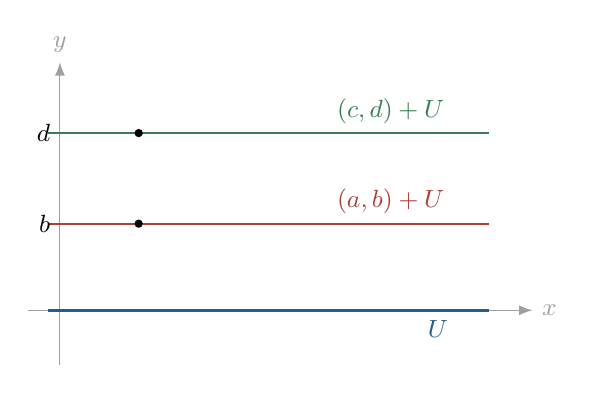
\begin{tikzpicture}[>=Latex,scale=1,every node/.style={font=\small}]
 \draw[->,gray!75] (-0.4,0)--(6,0) node[right] {\(x\)};
 \draw[->,gray!75] (0,-0.7)--(0,3.15) node[above] {\(y\)};
 \draw[very thick,manifoldblue] (-0.15,0)--(5.45,0);
 \draw[thick,manifoldred] (-0.15,1.10)--(5.45,1.10);
 \draw[thick,manifoldgreen] (-0.15,2.25)--(5.45,2.25);
 \node[manifoldblue,below] at (4.8,0) {\(U\)};
 \node[manifoldred,above] at (4.20,1.10) {\((a,b)+U\)};
 \node[manifoldgreen,above] at (4.20,2.25) {\((c,d)+U\)};
 \node[left] at (0,1.10) {\(b\)};
 \node[left] at (0,2.25) {\(d\)};
 \fill (1.0,1.10) circle (1.5pt);
 \fill (1.0,2.25) circle (1.5pt);
\end{tikzpicture}
\caption{Dwie różne warstwy względem
\(U=\mathbb R\times\{0\}\). Ich suma
mnogościowa jest podzbiorem \(\mathbb R^2\),
natomiast każda z nich jest jednym
elementem przestrzeni ilorazowej.}
\label{fig:lin2-warstwy-r2}
\end{figure}

\begin{stwierdzenie}[Przypadki skrajne ilorazu]
\label{prop:lin2-iloraz-przypadki}
Dla każdej przestrzeni wektorowej \(V\)
zachodzą naturalne izomorfizmy
\(V/\{0_V\}\cong V\) oraz \(V/V\cong\{0\}\).
\end{stwierdzenie}
\begin{proof}
Gdy \(U=\{0_V\}\), każda warstwa jest
jednoelementowym zbiorem \(v+\{0_V\}=\{v\}\),
a odwzorowanie \(\{v\}\mapsto v\)
jest liniową bijekcją.
Gdy \(U=V\), każda warstwa jest równa \(V\),
więc iloraz ma dokładnie jeden element.
Jest zatem przestrzenią zerową.
\end{proof}

\begin{twierdzenie}[Uniwersalna własność przestrzeni ilorazowej]
\label{thm:lin2-wlasnosc-ilorazu}
Niech \(V,Z\) będą przestrzeniami wektorowymi
nad \(K\), \(U\subseteq V\) podprzestrzenią,
a \(T\colon V\to Z\) odwzorowaniem liniowym,
które spełnia \(T(u)=0_Z\) dla każdego \(u\in U\).
Wówczas istnieje dokładnie jedno odwzorowanie
liniowe \(\overline T\colon V/U\to Z\) takie, że
\[
 \overline T\circ\pi_U=T.
\]
Określa je wzór \(\overline T(v+U)=T(v)\).
\end{twierdzenie}
\begin{proof}
Jeśli \(v+U=w+U\), to
\(v-w\in U\) na mocy
Lematu~\ref{lem:lin2-warstwy}.
Stąd
\(T(v)-T(w)=T(v-w)=0_Z\),
czyli \(T(v)=T(w)\).
Wzór na \(\overline T\) jest więc
dobrze określony.
Dla \(a,b\in K\) oraz \(v,w\in V\)
mamy
\[
 \overline T(a(v+U)+b(w+U))
 =\overline T((av+bw)+U)
 =T(av+bw)
 =aT(v)+bT(w).
\]
Dowodzi to liniowości.
Równość \(\overline T\circ\pi_U=T\)
zachodzi dla każdego \(v\) wprost
z definicji.
Jeśli \(S\colon V/U\to Z\) jest innym
odwzorowaniem z \(S\circ\pi_U=T\),
to dla dowolnej warstwy \(v+U\)
otrzymujemy \(S(v+U)=S(\pi_U(v))=T(v)\).
Zatem \(S=\overline T\).
\end{proof}

\section{Dopełnienia algebraiczne i wymiar ilorazu}
\label{sec:lin2-dopelnienia}

\begin{definicja}[Dopełnienie podprzestrzeni]
\label{def:lin2-dopelnienie}
Podprzestrzeń \(W\subseteq V\) nazywamy
\emph{dopełnieniem algebraicznym}
podprzestrzeni \(U\subseteq V\), jeśli
\(V=U\oplus W\); czyli \(U+W=V\)
oraz \(U\cap W=\{0_V\}\).
\end{definicja}

\begin{twierdzenie}[Istnienie dopełnienia algebraicznego]
\label{thm:lin2-istnienie-dopelnienia}
Przyjmijmy aksjomat wyboru.
Niech \(U\subseteq V\) będzie podprzestrzenią.
Wówczas istnieje podprzestrzeń \(W\subseteq V\)
taka, że \(V=U\oplus W\).
Jeżeli \(V\) jest skończenie wymiarowa,
twierdzenie nie wymaga aksjomatu wyboru.
\end{twierdzenie}
\begin{proof}
Weźmy bazę Hamela \(B_U\) przestrzeni \(U\).
Z twierdzenia o rozszerzaniu bazy
(Twierdzenie~\ref{thm:lin-istnienie-bazy-zorn})
istnieje baza \(B\) całej \(V\)
taka, że \(B_U\subseteq B\).
Niech \(C=B\setminus B_U\) oraz
\(W=\operatorname{span}(C)\).
Ponieważ \(B=B_U\sqcup C\) rozpina \(V\),
mamy \(U+W=V\).
Jeśli \(v\in U\cap W\), to
\[
 v=\sum_{b\in F}a_bb=\sum_{c\in G}d_cc,
 \quad F\subseteq B_U,\ G\subseteq C\text{ skończone}.
\]
Po przeniesieniu składników na jedną stronę
otrzymujemy równość, do której stosujemy
warunek niezależności liniowej bazy \(B\).
Wszystkie współczynniki są więc zerowe,
czyli \(v=0_V\).
Zatem \(U\cap W=\{0_V\}\), co dowodzi
\(V=U\oplus W\).
Jeśli \(V\) ma skończoną bazę, także \(U\)
ma skończoną bazę, a jej rozszerzenie
można wykonać skończoną procedurą
z Twierdzenia~\ref{thm:lin-uzupelnianie-skonczone}.
\end{proof}

\begin{twierdzenie}[Iloraz i dopełnienie]
\label{thm:lin2-iloraz-dopelnienie}
Jeżeli \(V=U\oplus W\), to
\[
 \Theta\colon W\longrightarrow V/U,\qquad
 w\longmapsto w+U
\]
jest izomorfizmem przestrzeni wektorowych.
Przyjmując aksjomat wyboru,
dla każdej podprzestrzeni \(U\subseteq V\)
otrzymujemy równość kardynalną
\[
 \dim_KV=\dim_KU+\dim_K(V/U).
\]
W przypadku skończenie wymiarowym
wynika z niej
\(\dim_K(V/U)=\dim_KV-\dim_KU\).
\end{twierdzenie}
\begin{proof}
Liniowość \(\Theta\) jest ograniczeniem
odwzorowania ilorazowego \(\pi_U\).
Jeżeli \(\Theta(w)=0_{V/U}\),
to \(w\in U\) na mocy
Twierdzenia~\ref{thm:lin2-struktura-ilorazu}.
Ponieważ \(w\in W\) i \(U\cap W=\{0_V\}\),
otrzymujemy \(w=0_V\), więc \(\Theta\)
jest iniektywne.
Niech \(v+U\in V/U\). Z rozkładu
\(v=u+w\), gdzie \(u\in U\), \(w\in W\),
otrzymujemy \(v+U=w+U=\Theta(w)\),
co dowodzi surjektywności.

Z Twierdzenia~\ref{thm:lin2-istnienie-dopelnienia}
wybieramy algebraiczne dopełnienie \(W\).
Izomorfizm \(\Theta\) przenosi każdą bazę
\((w_j)_{j\in J}\) przestrzeni \(W\)
na bazę \((\Theta(w_j))_{j\in J}\) ilorazu:
jego surjektywność daje rozpinanie,
gdyż każda warstwa jest obrazem pewnego
wektora z \(W\), a ten jest skończoną
kombinacją elementów bazy.
Jeśli
\(\sum_{j\in F}a_j\Theta(w_j)=0_{V/U}\),
to z liniowości otrzymujemy
\(\Theta(\sum_{j\in F}a_jw_j)=0_{V/U}\).
Iniektywność \(\Theta\) daje
\(\sum_{j\in F}a_jw_j=0_V\),
a niezależność rodziny \((w_j)_{j\in J}\)
wymusza \(a_j=0_K\) dla każdego \(j\in F\).
Tak więc rodzina obrazów jest bazą
indeksowaną przez ten sam zbiór \(J\).
Stąd \(\dim_KW=\dim_K(V/U)\).
Stosując następnie
Twierdzenie~\ref{thm:lin2-wymiar-sumy-prostej},
otrzymujemy
\[
 \dim_KV=\dim_KU+\dim_KW
 =\dim_KU+\dim_K(V/U).
\]
Jeżeli \(V\) jest skończenie wymiarowa,
bazy \(U\) i \(W\) otrzymujemy z twierdzeń
skończenie wymiarowych bez aksjomatu wyboru.
Połączenie tych baz jest bazą \(V=U\oplus W\):
rozpinanie wynika z równości \(U+W=V\),
a warunek niezależności liniowej
z \(U\cap W=\{0_V\}\) i niezależności
obu baz. Zatem liczba jej wektorów jest
sumą liczb wektorów obu baz.
Możemy więc w tym przypadku odjąć
\(\dim_KU\) i otrzymać wskazany wzór,
nie odwołując się do aksjomatu wyboru.
\end{proof}

\begin{przyklad}[Niekanoniczność dopełnienia]
\label{prz:lin2-dopelnienia}
W \(\mathbb R^2\) niech \(U=\mathbb R\times\{0\}\).
Zarówno \(W_1=\operatorname{span}\{(0,1)\}\),
jak i \(W_2=\operatorname{span}\{(1,1)\}\)
są dopełnieniami \(U\).
Istotnie, z równości
\(a(1,0)+b(0,1)=0\) wynika \(a=b=0\),
podobnie z
\(a(1,0)+b(1,1)=(a+b,b)=0\)
wynika \(a=b=0\).
W obu przypadkach generatory rozpinają
\(\mathbb R^2\), bo
\((x,y)=x(1,0)+y(0,1)
=(x-y)(1,0)+y(1,1)\).
Podprzestrzenie \(W_1\) i \(W_2\)
są różne, choć obie są izomorficzne
z \(\mathbb R^2/U\). Oznacza to, że
\emph{dopełnienie algebraiczne nie jest
jednoznacznie wyznaczone} przez samo zawieranie
\(U\subseteq V\). Nie utożsamiamy tego
spostrzeżenia z osobnym twierdzeniem o braku
konstrukcji naturalnej: samo wskazanie dwóch
różnych dopełnień nie wystarczałoby
do udowodnienia takiej tezy.
\end{przyklad}

\begin{twierdzenie}[Twierdzenie o ilorazie sumy]
\label{thm:lin2-iloraz-sumy}
Niech \(U,W\subseteq V\) będą podprzestrzeniami.
Wtedy istnieje naturalny izomorfizm
\[
 U/(U\cap W)\ \cong\ (U+W)/W,
 \qquad u+(U\cap W)\longmapsto u+W.
\]
\end{twierdzenie}
\begin{proof}
Określmy odwzorowanie
\(T\colon U\to (U+W)/W\),
\(T(u)=u+W\).
Jest ono liniowe, jako ograniczenie
kanonicznego odwzorowania ilorazowego
\(U+W\to(U+W)/W\).
Ponadto \(T(u)=0\) dokładnie wtedy,
gdy \(u\in W\); ponieważ \(u\in U\),
jest to równoważne \(u\in U\cap W\).
W szczególności \(T\) jest zerowe
na \(U\cap W\).
Z własności uniwersalnej
(Twierdzenie~\ref{thm:lin2-wlasnosc-ilorazu})
otrzymujemy liniowe odwzorowanie
\(\overline T\colon U/(U\cap W)\to (U+W)/W\)
dane wzorem z tezy.

Jeśli \(\overline T(u+(U\cap W))=0\),
to \(u\in W\), a więc \(u\in U\cap W\).
Oznacza to, że wyjściowa warstwa jest zerowa,
czyli \(\overline T\) jest iniektywne.
Jeśli \(x+W\in(U+W)/W\), to
\(x=u+w\) dla pewnych \(u\in U,w\in W\).
Stąd \(x+W=u+W=\overline T(u+(U\cap W))\).
Odwzorowanie jest więc surjektywne
i stanowi izomorfizm.
\end{proof}

\begin{przyklad}[Iloraz wielomianów przez wielomiany stałe]
\label{prz:lin2-iloraz-wielomiany}
Niech \(V=K[X]\), \(U=K[X]_{\leq0}\).
Podprzestrzeń \(U\) składa się ze stałych wielomianów,
a \(W=\{p\in K[X]:p(0)=0_K\}\)
ze wszystkich wielomianów o zerowym wyrazie stałym.
Dla każdego \(p(X)=a_0+\sum_{j=1}^d a_jX^j\)
(z umową, że suma jest pusta przy \(d=0\))
mamy \(p=a_0+q\), gdzie
\(q(X)=\sum_{j=1}^d a_jX^j\in W\). Wspólnym elementem
\(U\cap W\) jest tylko wielomian zerowy,
zatem \(K[X]=U\oplus W\).
Iloraz \(K[X]/K[X]_{\leq0}\) jest więc
izomorficzny z \(W\), która ma bazę
\((X,X^2,X^3,\ldots)\).
Iloraz nadal ma wymiar \(\aleph_0\),
tak jak przestrzeń wyjściowa.
\end{przyklad}

\section{Podsumowanie}
\label{sec:lin2-podsumowanie}

Suma zbiorów \(U\cup W\) i suma algebraiczna
podprzestrzeni \(U+W\) są różnymi konstrukcjami.
Suma prosta oznacza jednoznaczny rozkład na składniki
należące do odpowiednich podprzestrzeni.
W przestrzeni ilorazowej \(V/U\) utożsamiamy wektory,
których różnica należy do \(U\); otrzymane warstwy
są wektorami nowej przestrzeni.
Przy założeniu aksjomatu wyboru każda podprzestrzeń
posiada dopełnienie algebraiczne, a wymiar
zachowuje się zgodnie z dodawaniem kardynalnym:
\[
 \dim_K(U+W)+\dim_K(U\cap W)=\dim_KU+\dim_KW,
 \qquad
 \dim_KV=\dim_KU+\dim_K(V/U).
\]
Przy wymiarach skończonych wolno z tych równości
odjąć odpowiednie składniki, natomiast
w przypadku nieskończonym nie wolno tego robić
bez dodatkowych warunków.

\chapter{Odwzorowania liniowe, jądro i obraz}
\label{ch:lin3-odwzorowania-liniowe}
\index{odwzorowanie liniowe@Odwzorowanie liniowe}
\index{jadro odwzorowania@Jądro odwzorowania liniowego}
\index{obraz odwzorowania@Obraz odwzorowania liniowego}

\noindent\textbf{Cel rozdziału.}
W Rozdziale~\ref{ch:lin-przestrzenie-wektorowe}
poznaliśmy przestrzenie wektorowe, bazy Hamela i współrzędne,
a w Rozdziale~\ref{ch:lin2-wymiar-sumy-ilorazy}
sumy proste, wymiar kardynalny i przestrzenie ilorazowe.
Teraz badamy odwzorowania zachowujące strukturę liniową.
Wskażemy, jak ich jądro mierzy utratę informacji,
jak obraz opisuje osiągalne wartości i dlaczego
iloraz przez jądro jest izomorficzny z obrazem.
Wyznaczymy również przestrzeń wszystkich odwzorowań
liniowych i omówimy projekcje.

W całym rozdziale \(K\) jest ciałem, \(0_K\neq1_K\),
a wszystkie przestrzenie wektorowe są nad \(K\).
Nie zakładamy skończonej wymiarowości, o ile nie
zostanie ona wyraźnie wskazana. Suma wektorów
indeksowana nieskończonym zbiorem oznacza
wyłącznie sumę o skończonym nośniku.
Przy wynikach wymagających wyboru baz dowolnych
przestrzeni nieskończenie wymiarowych
jawnie przyjmujemy aksjomat wyboru.

\section{Definicja i pierwsze własności}
\label{sec:lin3-definicja}

\begin{definicja}[Odwzorowanie liniowe]
\label{def:lin3-odwzorowanie-liniowe}
Niech \(V,W\) będą przestrzeniami wektorowymi nad \(K\).
Odwzorowanie \(T\colon V\to W\) nazywamy
\emph{liniowym}, jeżeli dla dowolnych \(v,w\in V\)
i \(a\in K\) zachodzą
\[
 T(v+w)=T(v)+T(w),\qquad T(av)=aT(v).
\]
Pierwszy warunek nazywamy \emph{addytywnością},
a drugi \emph{jednorodnością}.
\end{definicja}

\begin{stwierdzenie}[Kryterium jednej kombinacji]
\label{prop:lin3-kryterium}
Niech \(V,W\) będą przestrzeniami wektorowymi
nad \(K\), a \(T\colon V\to W\) odwzorowaniem.
Jest ono liniowe wtedy i tylko wtedy, gdy
dla wszystkich \(a,b\in K\) oraz \(v,w\in V\) zachodzi
\[
 T(av+bw)=aT(v)+bT(w).
\]
\end{stwierdzenie}
\begin{proof}
Jeżeli \(T\) jest liniowe, to stosujemy
addytywność do \(av+bw\), a następnie jednorodność
do każdego składnika. W przeciwnym kierunku
ustawmy \(a=b=0_K\); otrzymujemy \(T(0_V)=0_W\).
Następnie dla \(a=b=1_K\) otrzymujemy
\(T(v+w)=T(v)+T(w)\).
Wreszcie przy \(b=0_K\) dostajemy
\(T(av)=aT(v)+0_KT(w)=aT(v)\).
Oba warunki definicji są więc spełnione.
\end{proof}

\begin{lemat}[Podstawowe tożsamości]
\label{lem:lin3-podstawowe}
Niech \(T\colon V\to W\) będzie liniowe,
gdzie \(V,W\) są przestrzeniami wektorowymi nad \(K\).
Wtedy \(T(0_V)=0_W\), \(T(-v)=-T(v)\) dla
każdego \(v\in V\), a dla dowolnych
\(m\in\mathbb N_0\), \(a_1,\ldots,a_m\in K\)
i \(v_1,\ldots,v_m\in V\) mamy
\[
 T\left(\sum_{j=1}^m a_jv_j\right)
   =\sum_{j=1}^m a_jT(v_j).
\]
Równość obejmuje przypadek \(m=0\).
\end{lemat}
\begin{proof}
Z jednorodności \(T(0_Kv)=0_KT(v)=0_W\).
Podstawiając skalar \(-1_K\), otrzymujemy
\(T(-v)=(-1_K)T(v)=-T(v)\).
Równość dla sumy jednego składnika wynika
z jednorodności. Jeżeli zachodzi dla \(m\),
to dla \(m+1\) używamy addytywności,
a następnie założenia indukcyjnego:
\[
 T\left(\sum_{j=1}^{m+1}a_jv_j\right)
 =T\left(\sum_{j=1}^{m}a_jv_j\right)
   +T(a_{m+1}v_{m+1})
 =\sum_{j=1}^{m+1}a_jT(v_j).
\]
Przy \(m=0\) obie strony są wektorami zerowymi.
\end{proof}

\begin{przyklad}[Odwzorowania współrzędnych]
\label{prz:lin3-wspolrzedne}
Niech \(K\) będzie dowolnym ciałem i oznaczmy
\(2_K:=1_K+1_K\).
Odwzorowanie
\[
 T\colon K^2\longrightarrow K^3,\qquad
 T(x,y)=(x+y,x-y,2_Kx)
\]
jest liniowe. Istotnie, w każdej współrzędnej
otrzymujemy liniową kombinację \(x,y\).
Dla \(u=(x,y)\), \(v=(s,t)\) i \(a,b\in K\)
pierwsza współrzędna \(T(au+bv)\) wynosi
\(a(x+y)+b(s+t)\); w dwóch pozostałych
rachunek jest analogiczny. Daje to
\(T(au+bv)=aT(u)+bT(v)\).
W przypadku charakterystyki \(2\)
trzecia współrzędna jest zawsze zerowa;
nie wpływa to na liniowość odwzorowania.
\end{przyklad}

\begin{przyklad}[Przykłady niebędące liniowymi]
\label{prz:lin3-nieliniowe}
Niech \(S\colon V\to W\) będzie liniowe
i niech \(w_0\in W\setminus\{0_W\}\).
Odwzorowanie afiniczne \(A(v)=S(v)+w_0\)
nie jest liniowe, gdyż \(A(0_V)=w_0\neq0_W\).
Także \(f\colon\mathbb R\to\mathbb R\),
\(f(x)=x^2\), nie jest liniowe:
\(f(1+1)=4\), natomiast \(f(1)+f(1)=2\).
Ostatnie równanie jest kontrprzykładem
do addytywności, a nie tylko do jednorodności.
\end{przyklad}

\section{Odwzorowanie liniowe wyznaczone na bazie}
\label{sec:lin3-baza}

\begin{twierdzenie}[Przedłużanie zadanych wartości na bazie]
\label{thm:lin3-przedluzenie-z-bazy}
Niech \(V,W\) będą przestrzeniami wektorowymi nad \(K\),
\(B=(b_i)_{i\in I}\) bazą Hamela \(V\), a
\((w_i)_{i\in I}\) dowolną rodziną wektorów \(W\).
Wtedy istnieje dokładnie jedno odwzorowanie liniowe
\(T\colon V\to W\) takie, że \(T(b_i)=w_i\)
dla każdego \(i\in I\). Określa je wzór
\[
 T\left(\sum_{i\in F}a_ib_i\right)
   =\sum_{i\in F}a_iw_i,
 \qquad F\subseteq I\text{ skończony},\quad a_i\in K.
\]
Jeżeli baza \(B\) jest już dana, twierdzenie
nie wymaga aksjomatu wyboru.
\end{twierdzenie}
\begin{proof}
Każdy \(v\in V\) ma dokładnie jedną rodzinę
współczynników w bazie \(B\), o skończonym nośniku,
na mocy Twierdzenia~\ref{thm:lin-wspolrzedne-hamela}.
Zatem prawa strona wzoru jest dobrze określona:
różne przedstawienia tego samego \(v\),
po dopisaniu zer, mają identyczne współczynniki.
Otrzymujemy więc odwzorowanie \(T\colon V\to W\).

Jeśli \(v=\sum_{i\in F}a_ib_i\) i
\(u=\sum_{i\in G}c_ib_i\), to dopisujemy zera
poza odpowiednimi nośnikami. Dla \(p,q\in K\)
współczynniki \(pv+qu\) względem \(B\)
wynoszą \(pa_i+qc_i\) dla \(i\in F\cup G\).
Stąd
\[
 \begin{aligned}
 T(pv+qu)
 &=\sum_{i\in F\cup G}(pa_i+qc_i)w_i\\
 &=p\sum_{i\in F}a_iw_i
   +q\sum_{i\in G}c_iw_i
 =pT(v)+qT(u).
 \end{aligned}
\]
Odwzorowanie jest liniowe i spełnia
\(T(b_i)=w_i\), gdyż współrzędne \(b_i\)
są równe \(1_K\) przy \(i\) i zerowe poza \(i\).

Jeśli \(S\colon V\to W\) jest innym odwzorowaniem
liniowym o tych samych wartościach na bazie,
to dla dowolnego \(v=\sum_{i\in F}a_ib_i\)
z Lematu~\ref{lem:lin3-podstawowe} otrzymujemy
\[
 S(v)=\sum_{i\in F}a_iS(b_i)
      =\sum_{i\in F}a_iw_i=T(v).
\]
Zatem \(S=T\). Przy \(I=\varnothing\)
przestrzeń \(V\) jest zerowa, a jedynym
odwzorowaniem liniowym \(V\to W\)
jest odwzorowanie zerowe; powyższy argument
obejmuje również ten przypadek.
\end{proof}

\begin{wniosek}[Zgodność na generatorach]
\label{cor:lin3-zgodnosc-na-generatorach}
Niech \(V,W\) będą przestrzeniami wektorowymi
nad \(K\), a \(S,T\colon V\to W\)
odwzorowaniami liniowymi. Jeżeli
\(A\subseteq V\) rozpina \(V\) i \(S(a)=T(a)\)
dla każdego \(a\in A\), to \(S=T\).
\end{wniosek}
\begin{proof}
Dla każdego \(v\in V\) istnieją
\(m\in\mathbb N_0\), skalary \(c_j\in K\)
i wektory \(a_j\in A\), \(1\leq j\leq m\),
takie, że \(v=\sum_{j=1}^{m}c_ja_j\).
Liniowość obu odwzorowań i ich zgodność
na \(A\) dają
\(S(v)=\sum_jc_jS(a_j)=\sum_jc_jT(a_j)=T(v)\).
Dotyczy to również \(V=\{0_V\}\)
i pustego zbioru generatorów.
\end{proof}

\begin{przyklad}[Dwa operatory na wielomianach]
\label{prz:lin3-przesuniecia-wielomianow}
Niech \(V=K[X]\) oraz \(B=(1,X,X^2,\ldots)\).
Wybór \(T(X^n)=X^{n+1}\) dla \(n\in\mathbb N_0\)
wyznacza dokładnie jedno odwzorowanie liniowe,
a z jego wzoru wynika \(T(p)=Xp\).
Z kolei wybór \(R(1)=0\) oraz
\(R(X^{n+1})=X^n\) dla \(n\in\mathbb N_0\)
wyznacza liniowe odwzorowanie
\[
 R(p)=\frac{p(X)-p(0)}{X}.
\]
Prawa strona oznacza wielomian, ponieważ
licznik ma zerowy wyraz stały.
Dla \(p=\sum_{j=0}^{d}a_jX^j\)
obliczamy \(R(p)=\sum_{j=1}^{d}a_jX^{j-1}\).
W szczególności \(R(T(p))=p\), ale
\(T(R(p))=p-p(0)\); oba złożenia
nie muszą być równe.
\end{przyklad}

\section{Jądro, obraz i warunki iniektywności}
\label{sec:lin3-jadro-obraz}

\begin{definicja}[Jądro i obraz]
\label{def:lin3-jadro-obraz}
Niech \(T\colon V\to W\) będzie odwzorowaniem
liniowym przestrzeni wektorowych nad \(K\).
Przez \emph{jądro} i \emph{obraz} rozumiemy zbiory
\[
 \ker T=\{v\in V:T(v)=0_W\},\qquad
 \operatorname{im}T=\{T(v):v\in V\}\subseteq W.
\]
Jądro jest zbiorem wektorów tracących
informację pod działaniem \(T\),
a obraz zbiorem wektorów osiągalnych w \(W\).
\end{definicja}

\begin{twierdzenie}[Jądro i obraz są podprzestrzeniami]
\label{thm:lin3-jadro-obraz-podprzestrzenie}
Niech \(T\colon V\to W\) będzie odwzorowaniem
liniowym przestrzeni wektorowych nad \(K\).
Wtedy \(\ker T\) jest podprzestrzenią \(V\),
a \(\operatorname{im}T\) jest podprzestrzenią \(W\).
\end{twierdzenie}
\begin{proof}
Wektor \(0_V\) należy do \(\ker T\),
ponieważ \(T(0_V)=0_W\).
Dla \(v,u\in\ker T\) oraz \(a,b\in K\)
otrzymujemy \(T(av+bu)=aT(v)+bT(u)=0_W\).
Zatem \(av+bu\in\ker T\), co na mocy
kryterium podprzestrzeni pokazuje pierwszą tezę.

Obraz zawiera \(0_W=T(0_V)\).
Jeśli \(y_1=T(v_1)\), \(y_2=T(v_2)\)
należą do obrazu, to
\(ay_1+by_2=T(av_1+bv_2)\)
również do niego należy.
Obraz jest więc podprzestrzenią \(W\).
\end{proof}

\begin{stwierdzenie}[Obrazy generatorów i przeciwobrazy podprzestrzeni]
\label{prop:lin3-generatory-przeciwobrazy}
Niech \(V,W\) będą przestrzeniami wektorowymi
nad \(K\), \(T\colon V\to W\) odwzorowaniem liniowym,
a \(A\subseteq V\) dowolnym zbiorem.
Wtedy
\[
 T(\operatorname{span}(A))
      =\operatorname{span}(T(A)).
\]
Jeżeli \(Z\subseteq W\) jest podprzestrzenią,
to \(T^{-1}(Z)=\{v\in V:T(v)\in Z\}\)
jest podprzestrzenią \(V\).
\end{stwierdzenie}
\begin{proof}
Dla \(v=\sum_{j=1}^m a_ja_j\), \(a_j\in A\),
liniowość daje \(T(v)=\sum_{j=1}^m a_jT(a_j)\),
a więc zawieranie z lewej do prawej.
Każdy wektor prawej strony ma postać
\(\sum_{j=1}^m a_jT(a_j)\), która jest obrazem
wektora \(\sum_{j=1}^m a_ja_j\in\operatorname{span}(A)\).
Stąd także zawieranie odwrotne.

Ponieważ \(T(0_V)=0_W\in Z\),
zbiór \(T^{-1}(Z)\) nie jest pusty.
Dla \(v,u\in T^{-1}(Z)\) i \(a,b\in K\)
mamy \(T(av+bu)=aT(v)+bT(u)\in Z\),
bo \(Z\) jest podprzestrzenią.
Spełnione jest więc kryterium podprzestrzeni.
\end{proof}

\begin{twierdzenie}[Jądro a iniektywność, obraz a surjektywność]
\label{thm:lin3-iniekcja-surjekcja}
Niech \(T\colon V\to W\) będzie odwzorowaniem
liniowym przestrzeni wektorowych nad \(K\).
Wtedy:
\begin{enumerate}[label=(\roman*)]
\item \(T\) jest iniektywne wtedy i tylko wtedy,
gdy \(\ker T=\{0_V\}\);
\item \(T\) jest surjektywne wtedy i tylko wtedy,
gdy \(\operatorname{im}T=W\);
\item \(T\) jest bijektywne wtedy i tylko wtedy,
gdy \(\ker T=\{0_V\}\) oraz \(\operatorname{im}T=W\).
\end{enumerate}
\end{twierdzenie}
\begin{proof}
Jeśli \(T\) jest iniektywne i \(v\in\ker T\),
to \(T(v)=0_W=T(0_V)\), a więc \(v=0_V\).
Odwrotnie, zakładając \(\ker T=\{0_V\}\),
z równości \(T(v)=T(u)\) dostajemy
\(T(v-u)=0_W\), czyli \(v-u=0_V\),
a zatem \(v=u\). Druga równoważność
wynika bezpośrednio z definicji surjektywności
i obrazu. Trzecia jest połączeniem pierwszych dwóch.
\end{proof}

\begin{przyklad}[Jądra i obrazy na wielomianach]
\label{prz:lin3-jadro-przesuniecia}
Dla operatorów \(T,R\colon K[X]\to K[X]\)
z Przykładu~\ref{prz:lin3-przesuniecia-wielomianow}
mamy
\[
 \ker T=\{0\},\quad
 \operatorname{im}T=XK[X],\qquad
 \ker R=K,\quad
 \operatorname{im}R=K[X].
\]
Pierwsze dwie równości wynikają z tego,
że iloczyn \(Xp\) jest zerowy tylko dla \(p=0\),
a wielomiany postaci \(Xp\) są dokładnie
wielomianami o zerowym wyrazie stałym.
W przypadku \(R\), równość \(R(p)=0\)
jest równoważna \(p=p(0)\), czyli stałości \(p\).
Dla dowolnego \(q\in K[X]\) mamy
\(R(Xq)=q\), więc \(R\) jest surjektywne.
Wynik pozostaje prawdziwy w każdej
charakterystyce ciała \(K\).
\end{przyklad}

\section{Wymiar jądra i obrazu}
\label{sec:lin3-twierdzenie-rzad}

\begin{definicja}[Rząd i wymiar jądra]
\label{def:lin3-rzad-nullity}
Niech \(T\colon V\to W\) będzie liniowe.
Przyjmując aksjomat wyboru dla dowolnych
przestrzeni wektorowych, definiujemy
\[
 \operatorname{rk}T:=\dim_K(\operatorname{im}T),
 \qquad
 \operatorname{null}T:=\dim_K(\ker T).
\]
Jeżeli \(V\) jest skończenie wymiarowa,
obie wielkości są liczbami naturalnymi
i można je określić bez aksjomatu wyboru.
\end{definicja}

\begin{twierdzenie}[Twierdzenie o wymiarze jądra i obrazu]
\label{thm:lin3-rzad-nullity}
Niech \(V,W\) będą przestrzeniami wektorowymi
nad \(K\), a \(T\colon V\to W\) odwzorowaniem liniowym.
Przy założeniu aksjomatu wyboru zachodzi
równość liczb kardynalnych
\[
 \dim_K V=\dim_K(\ker T)+\dim_K(\operatorname{im}T).
\]
Jeżeli \(V\) jest skończenie wymiarowa,
to \(\ker T\) i \(\operatorname{im}T\)
są skończenie wymiarowe, a ta równość
zachodzi również \emph{bez aksjomatu wyboru}.
W szczególności w tym przypadku
\(\operatorname{rk}T=\dim_KV-\operatorname{null}T\).
\end{twierdzenie}
\begin{proof}
Najpierw przyjmijmy aksjomat wyboru.
Wybierzmy bazę \(C\) jądra \(\ker T\)
i rozszerzmy ją do bazy \(B=C\sqcup D\)
całej przestrzeni \(V\).
Pokażemy, że rodzina \(T(D)=(T(d))_{d\in D}\)
jest bazą \(\operatorname{im}T\).

Dla \(y\in\operatorname{im}T\) istnieje \(v\in V\)
takie, że \(y=T(v)\). Rozwijając \(v\) w bazie \(B\),
otrzymujemy skończoną sumę
\[
 v=\sum_{c\in F}a_cc+\sum_{d\in G}b_dd,
 \qquad F\subseteq C,\ G\subseteq D.
\]
Ponieważ \(T(c)=0_W\) dla \(c\in C\),
mamy \(y=\sum_{d\in G}b_dT(d)\).
Rodzina \(T(D)\) rozpina więc obraz.

Aby sprawdzić warunek niezależności liniowej,
niech \(G\subseteq D\) będzie skończony i
\(\sum_{d\in G}b_dT(d)=0_W\).
Wektor \(u:=\sum_{d\in G}b_dd\) należy
wówczas do \(\ker T=\operatorname{span}(C)\).
Możemy zatem zapisać \(u=\sum_{c\in F}a_cc\)
dla pewnego skończonego \(F\subseteq C\).
Odejmując obie kombinacje otrzymujemy
\[
 \sum_{d\in G}b_dd-\sum_{c\in F}a_cc=0_V.
\]
Ponieważ \(B=C\sqcup D\) jest bazą,
wszystkie współczynniki \(b_d\) i \(a_c\)
muszą być zerowe. Dowodzi to niezależności \(T(D)\),
a zarazem zapewnia, że różne indeksy \(d\)
odpowiadają różnym wektorom \(T(d)\).

Mamy więc \(\dim_K(\operatorname{im}T)=|D|\),
\(\dim_K(\ker T)=|C|\) oraz
\(\dim_KV=|C|+|D|\).
Otrzymujemy wzór, bez odejmowania
nieskończonych liczb kardynalnych.

Jeśli \(V\) ma skończoną bazę, to
\(\ker T\) ma skończoną bazę \(C\)
na mocy wyników skończenie wymiarowych,
którą rozszerzamy skończoną procedurą
do bazy \(C\sqcup D\) przestrzeni \(V\).
Cały argument powyżej od tej chwili
stosuje się dosłownie, ale liczności
\(|C|\) i \(|D|\) są liczbami naturalnymi.
Nie użyto w nim aksjomatu wyboru.
\end{proof}

\begin{przyklad}[Wymiar jądra i obrazu konkretnego odwzorowania]
\label{prz:lin3-rzad-r3}
Niech \(T\colon\mathbb R^3\to\mathbb R^2\)
będzie dane wzorem
\[
 T(x,y,z)=(x+y,y+z).
\]
Jest liniowe, bo obie współrzędne są liniowymi
kombinacjami współrzędnych wejściowych.
Warunek \(T(x,y,z)=(0,0)\) daje układ
\(x=-y\), \(z=-y\). Zatem
\(\ker T=\operatorname{span}\{(-1,1,-1)\}\),
więc \(\operatorname{null}T=1\).
Z drugiej strony \(T(1,0,0)=(1,0)\)
i \(T(0,0,1)=(0,1)\), zatem
\(\operatorname{im}T=\mathbb R^2\),
czyli \(\operatorname{rk}T=2\).
Sprawdzamy wzór \(3=1+2\).
W szczególności \(T\) jest surjektywne,
lecz nie jest iniektywne.
\end{przyklad}

\begin{uwaga}[Wymiary nieskończone]
\label{rem:lin3-rzad-nieskonczony}
W przypadku nieskończenie wymiarowym
z równości
\(\dim_KV=\dim_K(\ker T)+\operatorname{rk}T\)
nie wolno odzyskiwać rzędu przez zwykłe
odejmowanie liczb kardynalnych.
Na przykład dla operatora \(T(p)=Xp\)
na \(K[X]\) mamy \(\ker T=\{0\}\)
i \(\operatorname{rk}T=\aleph_0\).
Dla operatora \(R\) z
Przykładu~\ref{prz:lin3-jadro-przesuniecia}
mamy \(\dim_K\ker R=1\)
i \(\operatorname{rk}R=\aleph_0\),
a mimo to oba wzory dają
\(\dim_KK[X]=\aleph_0\).
\end{uwaga}

\section{Pierwsze twierdzenie o izomorfizmie}
\label{sec:lin3-izomorfizm}

\begin{twierdzenie}[Pierwsze twierdzenie o izomorfizmie]
\label{thm:lin3-pierwsze-izo}
Niech \(V,W\) będą przestrzeniami wektorowymi
nad \(K\), a \(T\colon V\to W\)
odwzorowaniem liniowym. Wtedy
\[
 \widetilde T\colon V/\ker T
 \longrightarrow\operatorname{im}T,\qquad
 v+\ker T\longmapsto T(v)
\]
jest dobrze określonym izomorfizmem
przestrzeni wektorowych. Nie jest potrzebny
aksjomat wyboru.
\end{twierdzenie}
\begin{proof}
Najpierw sprawdzamy dobrą określoność.
Jeśli \(v+\ker T=u+\ker T\), to
z Lematu~\ref{lem:lin2-warstwy}
wynika \(v-u\in\ker T\).
Stąd \(T(v)-T(u)=T(v-u)=0_W\),
czyli \(T(v)=T(u)\).
Zatem wzór nie zależy od przedstawiciela warstwy.

Dla \(a,b\in K\) i \(v,u\in V\) otrzymujemy
\[
 \begin{aligned}
 \widetilde T\bigl(a(v+\ker T)+b(u+\ker T)\bigr)
  &=\widetilde T\bigl((av+bu)+\ker T\bigr)\\
  &=T(av+bu)=aT(v)+bT(u).
 \end{aligned}
\]
Jest to liniowość \(\widetilde T\).
Jeśli \(\widetilde T(v+\ker T)=0_W\),
to \(T(v)=0_W\), a więc \(v\in\ker T\).
Wówczas \(v+\ker T=\ker T=0_{V/\ker T}\).
Otrzymujemy iniektywność.
Wreszcie dla każdego \(y\in\operatorname{im}T\)
istnieje \(v\in V\) z \(y=T(v)\);
wtedy \(y=\widetilde T(v+\ker T)\).
Dowodzi to surjektywności.

Izomorfizm jest zatem określony wyłącznie
przez \(T\), bez wybierania dopełnienia
algebraicznego jądra ani bazy.
\end{proof}

\begin{figure}[!htbp]
\centering
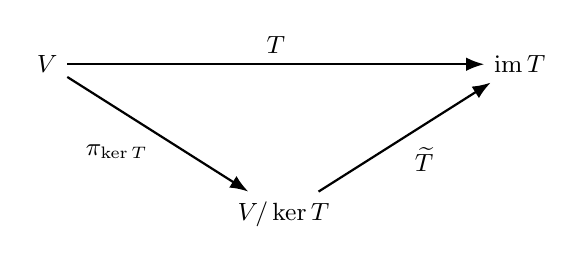
\begin{tikzpicture}[>=Latex,every node/.style={font=\small}]
 \node (V) at (0,1.9) {\(V\)};
 \node (W) at (6,1.9) {\(\operatorname{im}T\)};
 \node (Q) at (3,0) {\(V/\ker T\)};
 \draw[->,thick] (V)--node[above]{\(T\)} (W);
 \draw[->,thick] (V)--node[below left]{\(\pi_{\ker T}\)} (Q);
 \draw[->,thick] (Q)--node[below right]{\(\widetilde T\)} (W);
\end{tikzpicture}
\caption{Rozkład odwzorowania \(T\) na
odwzorowanie ilorazowe i izomorfizm na obraz:
\(T=\widetilde T\circ\pi_{\ker T}\).}
\label{fig:lin3-izo}
\end{figure}

\begin{stwierdzenie}[Kiedy odwzorowanie przechodzi do ilorazu?]
\label{prop:lin3-faktoryzacja-iloraz}
Niech \(V,W\) będą przestrzeniami wektorowymi
nad \(K\), niech \(U\subseteq V\) będzie
podprzestrzenią, a \(T\colon V\to W\) odwzorowaniem
liniowym. Istnieje liniowe odwzorowanie
\(S\colon V/U\to W\) z \(T=S\circ\pi_U\)
wtedy i tylko wtedy, gdy \(U\subseteq\ker T\).
Jeśli istnieje, jest jednoznaczne i spełnia
\(S(v+U)=T(v)\).
\end{stwierdzenie}
\begin{proof}
Jeśli \(T=S\circ\pi_U\), to dla \(u\in U\)
mamy \(\pi_U(u)=0_{V/U}\), stąd
\(T(u)=S(0_{V/U})=0_W\). Zatem
\(U\subseteq\ker T\).
Odwrotnie, jeśli \(U\subseteq\ker T\), to
\(T\) zeruje się na \(U\);
Twierdzenie~\ref{thm:lin2-wlasnosc-ilorazu}
daje istnienie i jednoznaczność \(S\)
oraz wskazany wzór.
\end{proof}

\begin{przyklad}[Wartość wielomianu w zerze]
\label{prz:lin3-ewaluacja}
Niech \(T\colon K[X]\to K\) będzie
dane przez \(T(p)=p(0)\).
Jest liniowe, bo
\((ap+bq)(0)=ap(0)+bq(0)\).
Wszystkie wielomiany o zerowym wyrazie
stałym są podzielne przez \(X\), zatem
\(\ker T=XK[X]\).
Odwzorowanie jest surjektywne:
dla \(c\in K\) wystarczy wziąć wielomian stały \(c\).
Pierwsze twierdzenie o izomorfizmie daje
\[
 K[X]/XK[X]\cong K,\qquad
 p+XK[X]\longmapsto p(0).
\]
Otrzymujemy jednoznaczne utożsamienie warstw
z wyrazami stałymi, bez wybierania
reprezentantów innych niż te użyte we wzorze.
\end{przyklad}

\section{Składanie i odwracalność odwzorowań liniowych}
\label{sec:lin3-skladanie}

\begin{stwierdzenie}[Składanie odwzorowań liniowych]
\label{prop:lin3-skladanie}
Niech \(U,V,W\) będą przestrzeniami
wektorowymi nad \(K\), a \(T\colon U\to V\),
\(S\colon V\to W\) odwzorowaniami liniowymi.
Wtedy złożenie \(S\circ T\colon U\to W\) jest liniowe,
\[
 \ker T\subseteq\ker(S\circ T),\qquad
 \operatorname{im}(S\circ T)\subseteq\operatorname{im}S.
\]
Ponadto odwzorowanie identycznościowe
\(\operatorname{id}_V\colon V\to V\)
jest liniowe i jest elementem neutralnym
składania tam, gdzie to składanie jest określone.
\end{stwierdzenie}
\begin{proof}
Dla \(u_1,u_2\in U\) i \(a,b\in K\)
mamy
\[
 (S\circ T)(au_1+bu_2)
 =S(aT(u_1)+bT(u_2))
 =aS(T(u_1))+bS(T(u_2)).
\]
Dowodzi to liniowości. Jeśli \(u\in\ker T\),
to \((S\circ T)(u)=S(0_V)=0_W\),
czyli \(u\in\ker(S\circ T)\).
Każdy wektor obrazu złożenia ma postać
\(S(T(u))\), więc należy do \(\operatorname{im}S\).
Dla odwzorowania identycznościowego
wszystkie warunki wynikają z
\(\operatorname{id}_V(av+bw)=av+bw
 =a\operatorname{id}_V(v)+b\operatorname{id}_V(w)\).
Równości \(T\circ\operatorname{id}_U=T\)
oraz \(\operatorname{id}_V\circ T=T\)
zachodzą punktowo.
\end{proof}

\begin{twierdzenie}[Izomorfizmy i odwzorowania odwrotne]
\label{thm:lin3-odwrotnosc}
Niech \(T\colon V\to W\) będzie odwzorowaniem
liniowym przestrzeni wektorowych nad \(K\).
Wówczas \(T\) jest bijektywne wtedy i tylko wtedy,
gdy istnieje liniowe \(S\colon W\to V\)
takie, że \(S\circ T=\operatorname{id}_V\)
i \(T\circ S=\operatorname{id}_W\).
W takim przypadku \(S=T^{-1}\) i \(T\)
nazywamy \emph{izomorfizmem}.
\end{twierdzenie}
\begin{proof}
Jeżeli \(S\) spełnia obie równości,
to z \(T(v)=T(u)\) wynika
\(v=S(T(v))=S(T(u))=u\), czyli \(T\)
jest iniektywne. Każdy \(w\in W\)
ma postać \(w=T(S(w))\), więc \(T\) jest surjektywne.

Odwrotnie, dla bijektywnego \(T\)
istnieje odwrotne odwzorowanie zbiorów
\(T^{-1}\colon W\to V\).
Dla \(w_1,w_2\in W\) i \(a,b\in K\)
niech \(v_i=T^{-1}(w_i)\).
Wówczas
\(T(av_1+bv_2)=aw_1+bw_2\).
Z iniektywności \(T\) otrzymujemy
\[
 T^{-1}(aw_1+bw_2)
 =aT^{-1}(w_1)+bT^{-1}(w_2).
\]
A więc odwrotność jest liniowa
i spełnia obie wymagane równości.
\end{proof}

\begin{stwierdzenie}[Izomorfizm zachowuje bazę i wymiar]
\label{prop:lin3-izomorfizm-baza}
Niech \(T\colon V\to W\) będzie izomorfizmem
przestrzeni wektorowych nad \(K\).
Jeżeli \(B\) jest bazą Hamela \(V\),
to \(T(B)\) jest bazą Hamela \(W\).
W szczególności przy aksjomacie wyboru
\(\dim_KV=\dim_KW\).
Jeżeli \(V,W\) są skończenie wymiarowe,
równość wymiarów nie wymaga aksjomatu wyboru.
\end{stwierdzenie}
\begin{proof}
Ponieważ \(T\) jest surjektywne,
\[
 W=T(V)=T(\operatorname{span}(B))
   =\operatorname{span}(T(B))
\]
na mocy Stwierdzenia~\ref{prop:lin3-generatory-przeciwobrazy}.
Jeżeli skończona kombinacja różnych elementów
\(T(b_1),\ldots,T(b_m)\), \(b_j\in B\),
jest zerowa, to
\(T(\sum_{j=1}^{m}a_jb_j)=0_W\).
Iniektywność \(T\) daje
\(\sum_{j=1}^{m}a_jb_j=0_V\),
a niezależność \(B\) wymusza \(a_j=0_K\)
dla wszystkich \(j\).
Odwzorowanie \(b\mapsto T(b)\) jest iniektywne
na \(B\), więc zachowuje też moc rodziny bazowej.
Przy skończonych bazach jest to równość liczb
naturalnych i nie wymaga wyboru.
\end{proof}

\begin{wniosek}[Kryterium bijektywności w równych wymiarach]
\label{cor:lin3-rownymiary}
Niech \(V,W\) będą skończenie wymiarowymi
przestrzeniami wektorowymi nad \(K\)
o tym samym wymiarze \(n\in\mathbb N_0\).
Wtedy dla każdego liniowego \(T\colon V\to W\)
następujące warunki są równoważne:
\(T\) jest iniektywne, \(T\) jest surjektywne,
\(T\) jest izomorfizmem.
\end{wniosek}
\begin{proof}
Z Twierdzenia~\ref{thm:lin3-rzad-nullity}
mamy \(n=\dim_K\ker T+\dim_K\operatorname{im}T\).
Jeżeli \(T\) jest iniektywne, to
\(\dim_K\ker T=0\), zatem obraz ma wymiar \(n\).
Jako podprzestrzeń \(W\) o tym samym wymiarze,
obraz musi być równy \(W\)
(Twierdzenie~\ref{thm:lin-wymiar-podprzestrzeni}).
Wtedy \(T\) jest surjektywne.
Jeżeli \(T\) jest surjektywne, to
\(\dim_K\operatorname{im}T=n\),
a więc wymiar jądra jest zerowy.
Przestrzeń o wymiarze zero jest zerowa,
więc \(T\) jest iniektywne.
Ostatnia równoważność wynika z definicji
izomorfizmu i Twierdzenia~\ref{thm:lin3-odwrotnosc}.
Przy \(n=0\) przestrzenie \(V,W\) są zerowe
i jedyne odwzorowanie liniowe jest izomorfizmem.
\end{proof}

\begin{przyklad}[Dlaczego wymiar skończony jest istotny?]
\label{prz:lin3-infty-nie-rownowazne}
Operatory \(T,R\colon K[X]\to K[X]\)
z Przykładu~\ref{prz:lin3-przesuniecia-wielomianow}
spełniają \(R\circ T=\operatorname{id}_{K[X]}\)
oraz \(T\circ R(p)=p-p(0)\).
Zatem \(T\) jest iniektywne, ale nie jest
surjektywne: żaden wielomian \(Xp\)
nie jest równy \(1\).
Natomiast \(R\) jest surjektywne,
ale nie jest iniektywne, bo \(R(1)=0\).
Mimo to dziedzina i przeciwdziedzina
obu odwzorowań mają ten sam nieskończony wymiar
\(\aleph_0\). Wniosek~\ref{cor:lin3-rownymiary}
nie przenosi się bez dodatkowych założeń
na przestrzenie nieskończenie wymiarowe.
\end{przyklad}

\section{Przestrzenie odwzorowań liniowych}
\label{sec:lin3-hom}

\begin{definicja}[Przestrzenie \(\operatorname{Hom}\) i \(\operatorname{End}\)]
\label{def:lin3-hom-end}
Dla przestrzeni wektorowych \(V,W\) nad \(K\)
oznaczamy przez
\[
 \operatorname{Hom}_K(V,W)
  :=\{T\colon V\to W:T\text{ jest liniowe}\}
\]
zbiór wszystkich odwzorowań liniowych.
Przez \(\operatorname{End}_K(V)=\operatorname{Hom}_K(V,V)\)
rozumiemy zbiór \emph{endomorfizmów} \(V\).
Na \(\operatorname{Hom}_K(V,W)\) określamy działania
\[
 (S+T)(v)=S(v)+T(v),\qquad
 (aT)(v)=aT(v).
\]
\end{definicja}

\begin{twierdzenie}[Przestrzeń liniowa odwzorowań]
\label{thm:lin3-hom-przestrzen}
Niech \(V,W\) będą przestrzeniami wektorowymi nad \(K\).
Zbiór \(\operatorname{Hom}_K(V,W)\)
z działaniami punktowymi jest przestrzenią wektorową nad \(K\).
Jeżeli \(\dim_KV=n\) i \(\dim_KW=m\)
są skończone, to
\[
 \dim_K\operatorname{Hom}_K(V,W)=mn.
\]
Druga część twierdzenia nie wymaga aksjomatu wyboru.
\end{twierdzenie}
\begin{proof}
Najpierw \(\operatorname{Hom}_K(V,W)\)
zawiera odwzorowanie zerowe.
Jeżeli \(S,T\) są liniowe i \(a,b\in K\),
to dla dowolnych \(v,u\in V\) i \(c,d\in K\)
\[
 \begin{aligned}
 (aS+bT)(cv+du)
  &=aS(cv+du)+bT(cv+du)\\
  &=c(aS+bT)(v)+d(aS+bT)(u).
 \end{aligned}
\]
Suma i iloczyn przez skalar pozostają więc liniowe.
Pozostałe aksjomaty przestrzeni wektorowej
wynikają z odpowiednich aksjomatów \(W\)
po podstawieniu dowolnego \(v\in V\).

Niech teraz \(B=(v_1,\ldots,v_n)\)
i \(C=(w_1,\ldots,w_m)\) będą bazami odpowiednio
\(V\) i \(W\).
Dla każdej pary \(1\leq i\leq n\),
\(1\leq j\leq m\) Twierdzenie~\ref{thm:lin3-przedluzenie-z-bazy}
daje jednoznaczne liniowe \(E_{ji}\colon V\to W\),
określone na bazie przez
\[
 E_{ji}(v_k)=
 \begin{cases}
   w_j,&k=i,\\
   0_W,&k\neq i.
 \end{cases}
\]
Pokażemy, że rodzina \((E_{ji})\) jest bazą
\(\operatorname{Hom}_K(V,W)\).

Dla dowolnego liniowego \(T\colon V\to W\)
rozwińmy \(T(v_i)=\sum_{j=1}^{m}a_{ji}w_j\).
Odwzorowania \(T\) oraz
\(\sum_{i=1}^{n}\sum_{j=1}^{m}a_{ji}E_{ji}\)
zgadzają się na każdym \(v_k\);
na mocy Wniosku~\ref{cor:lin3-zgodnosc-na-generatorach}
są więc równe. Dowodzi to rozpinania.

Jeżeli \(\sum_{i,j}c_{ji}E_{ji}=0\),
to po zastosowaniu obu stron do \(v_k\)
otrzymujemy \(\sum_{j=1}^{m}c_{jk}w_j=0_W\).
Niezależność bazy \(C\) daje
\(c_{jk}=0_K\) dla każdego \(j,k\).
Jest to warunek niezależności liniowej
rodziny \((E_{ji})\). Jej liczba elementów
wynosi \(mn\), co dowodzi wzoru.

Przy \(n=0\) istnieje tylko odwzorowanie zerowe
z \(V=\{0_V\}\) do \(W\); przy \(m=0\)
istnieje tylko odwzorowanie zerowe do \(W=\{0_W\}\).
W obu przypadkach \(\operatorname{Hom}_K(V,W)\)
jest przestrzenią zerową, a wzór daje \(mn=0\).
\end{proof}

\begin{stwierdzenie}[Algebra endomorfizmów]
\label{prop:lin3-end-algebra}
Niech \(V\) będzie przestrzenią wektorową nad \(K\).
Przestrzeń \(\operatorname{End}_K(V)\)
z dodawaniem i mnożeniem przez skalary
wykonywanymi punktowo oraz z mnożeniem
\(S\cdot T:=S\circ T\)
jest łączną algebrą nad \(K\) z jedynką
\(\operatorname{id}_V\).
W ogólności mnożenie nie jest przemienne.
\end{stwierdzenie}
\begin{proof}
Dzięki Stwierdzeniu~\ref{prop:lin3-skladanie}
złożenie endomorfizmów jest endomorfizmem.
Łączność wynika z łączności składania funkcji.
Dla \(S,T,R\in\operatorname{End}_K(V)\),
\(a\in K\) i \(v\in V\) mamy
\[
 \begin{aligned}
 ((S+T)\circ R)(v)&=S(R(v))+T(R(v)),\\
 (S\circ(T+R))(v)&=S(T(v)+R(v))
                  =S(T(v))+S(R(v)),\\
 ((aS)\circ T)(v)&=aS(T(v))
                  =(S\circ(aT))(v).
 \end{aligned}
\]
Są to rozdzielności i zgodność
mnożenia z mnożeniem przez skalary.
Jedynką jest odwzorowanie identycznościowe.

Aby zobaczyć, że nie musi zachodzić
przemienność, rozważmy na \(K^2\)
endomorfizmy \(P(x,y)=(x,0)\)
oraz \(Q(x,y)=(y,x)\).
Mamy \((P\circ Q)(1,0)=(0,0)\),
natomiast \((Q\circ P)(1,0)=(0,1)\).
Wobec \(1_K\neq0_K\) oba złożenia są różne.
\end{proof}

\section{Projekcje i sumy proste}
\label{sec:lin3-projekcje}

\begin{definicja}[Projekcja algebraiczna]
\label{def:lin3-projekcja}
Niech \(V\) będzie przestrzenią wektorową nad \(K\).
Endomorfizm \(P\colon V\to V\) nazywamy
\emph{projekcją algebraiczną}, jeśli
\(P^2=P\), gdzie \(P^2=P\circ P\).
\end{definicja}

\begin{twierdzenie}[Projekcje i rozkłady na sumę prostą]
\label{thm:lin3-projekcja-suma}
Niech \(V\) będzie przestrzenią wektorową nad \(K\)
i \(P\colon V\to V\) endomorfizmem.
Wtedy \(P^2=P\) wtedy i tylko wtedy, gdy
\[
 V=\operatorname{im}P\oplus\ker P
\]
oraz \(P\) jest identycznością na
\(\operatorname{im}P\).

Ponadto jeśli \(V=U\oplus W\)
dla podprzestrzeni \(U,W\subseteq V\),
to istnieje dokładnie jedna projekcja liniowa
\(P\colon V\to V\) spełniająca
\(P(u)=u\) dla \(u\in U\) i \(P(w)=0_V\)
dla \(w\in W\). Wówczas
\(\operatorname{im}P=U\) i \(\ker P=W\).
\end{twierdzenie}
\begin{proof}
Załóżmy \(P^2=P\). Każdy \(v\in V\)
ma rozkład
\[
 v=P(v)+(v-P(v)).
\]
Pierwszy składnik należy do obrazu,
a drugi do jądra, ponieważ
\(P(v-P(v))=P(v)-P^2(v)=0_V\).
Zatem \(V=\operatorname{im}P+\ker P\).
Jeżeli \(x\in\operatorname{im}P\cap\ker P\),
to \(x=P(y)\) dla pewnego \(y\in V\),
stąd \(P(x)=P^2(y)=P(y)=x\),
ale zarazem \(P(x)=0_V\).
Wobec tego \(x=0_V\), a suma jest prosta.
Rachunek \(P(P(y))=P(y)\) pokazuje również,
że \(P\) jest identycznością na obrazie.

W odwrotnym kierunku załóżmy,
że \(V=\operatorname{im}P\oplus\ker P\)
oraz \(P(x)=x\) dla \(x\in\operatorname{im}P\).
Dla każdego \(v\in V\) wektor \(P(v)\)
należy do obrazu, więc \(P^2(v)=P(v)\);
mamy zatem \(P^2=P\).

Niech teraz \(V=U\oplus W\).
Z Twierdzenia~\ref{thm:lin2-kryteria-sumy-prostej}
każdy \(v\in V\) ma dokładnie jeden rozkład
\(v=u+w\), \(u\in U,w\in W\).
Definiujemy \(P(v)=u\).
Dla \(v_i=u_i+w_i\) i \(a,b\in K\)
wektor \(av_1+bv_2\) ma rozkład
\((au_1+bu_2)+(aw_1+bw_2)\);
jednoznaczność daje
\(P(av_1+bv_2)=au_1+bu_2
 =aP(v_1)+bP(v_2)\).
Odwzorowanie jest więc liniowe.
Ponieważ \(P(u+w)=u\), mamy
\(P^2=P\), \(\operatorname{im}P=U\)
i \(\ker P=W\).
Każde inne odwzorowanie liniowe o wskazanych
wartościach na \(U\) i \(W\) musiałoby spełniać
\(Q(u+w)=Q(u)+Q(w)=u=P(u+w)\).
Dowodzi to jednoznaczności.
\end{proof}

\begin{przyklad}[Projekcja na oś]
\label{prz:lin3-projekcja-os}
W \(\mathbb R^2\) przyjmijmy
\(U=\mathbb R\times\{0\}\) oraz
\(W=\{0\}\times\mathbb R\).
Projekcja wzdłuż \(W\) na \(U\) jest dana wzorem
\[
 P(x,y)=(x,0).
\]
Wtedy \(P^2=P\), \(\operatorname{im}P=U\),
\(\ker P=W\) i \(\mathbb R^2=U\oplus W\).
Jeśli zamiast \(W\) wybierzemy
\(\operatorname{span}\{(1,1)\}\),
to otrzymamy inne dopełnienie \(U\)
i inną projekcję \(P'(x,y)=(x-y,0)\).
Potwierdza to niejednoznaczność dopełnień
z Przykładu~\ref{prz:lin2-dopelnienia}.
\end{przyklad}

\section{Podsumowanie}
\label{sec:lin3-podsumowanie}

Odwzorowanie liniowe jest wyznaczone jednoznacznie
przez wartości na ustalonej bazie Hamela.
Jego jądro i obraz są podprzestrzeniami,
a jądro charakteryzuje iniektywność.
W przypadku ogólnym przy aksjomacie wyboru
obowiązuje kardynalny wzór
\[
 \dim_KV=\dim_K\ker T+\dim_K\operatorname{im}T,
\]
który w skończonym wymiarze nie wymaga tego aksjomatu.
Zarazem zawsze, bez aksjomatu wyboru, mamy
kanoniczny izomorfizm
\(V/\ker T\cong\operatorname{im}T\).
Odwzorowania liniowe tworzą przestrzeń
\(\operatorname{Hom}_K(V,W)\), a endomorfizmy
można dodatkowo składać.
Projekcje algebraiczne opisują dokładnie
rozkłady przestrzeni na sumy proste
wzdłuż wskazanych dopełnień.

\chapter{Macierze odwzorowań liniowych i zmiana bazy}
\label{ch:lin4-macierze-zmiana-bazy}
\index{macierz@Macierz}
\index{macierz odwzorowania@Macierz odwzorowania liniowego}
\index{zmiana bazy@Zmiana bazy}

\noindent\textbf{Cel rozdziału.}
W Rozdziale~\ref{ch:lin-przestrzenie-wektorowe}
zdefiniowaliśmy współrzędne wektorów,
a w Rozdziale~\ref{ch:lin3-odwzorowania-liniowe}
zbadaliśmy odwzorowania liniowe, ich jądra i obrazy.
Macierz pozwala zapisać każde odwzorowanie liniowe
między przestrzeniami skończenie wymiarowymi
za pomocą skończonej tablicy skalarów.
Pokażemy, dlaczego kolumny macierzy są obrazami
wektorów bazowych, skąd bierze się wzór na mnożenie
macierzy i jak zmienia się zapis operatora
przy zmianie baz.

W całym rozdziale \(K\) jest ciałem,
\(0_K\neq1_K\), a wszystkie przestrzenie wektorowe
rozpatrujemy nad \(K\). Jeśli w danym twierdzeniu
występują dwie bazy, traktujemy je jako
\emph{uporządkowane} rodziny wektorów.
Przyjmujemy konwencję, że współrzędne wektora
zapisujemy w kolumnie. Złożenie \(S\circ T\)
oznacza najpierw zastosowanie \(T\), a potem \(S\).
Wyniki tego rozdziału dotyczą wymiarów skończonych;
ich dowody nie wymagają aksjomatu wyboru.

\section{Macierze jako prostokątne tablice skalarów}
\label{sec:lin4-definicja-macierzy}

\begin{definicja}[Macierz i jej rozmiar]
\label{def:lin4-macierz}
Niech \(m,n\in\mathbb N_0\).
\emph{Macierzą} o \(m\) wierszach i \(n\) kolumnach
nad \(K\) nazywamy rodzinę
\(A=(a_{ij})_{1\leq i\leq m,\ 1\leq j\leq n}\)
skalarów \(a_{ij}\in K\).
Zbiór wszystkich takich macierzy oznaczamy
przez \(\operatorname{Mat}_{m\times n}(K)\).
Dwie macierze są równe wtedy i tylko wtedy,
gdy mają ten sam rozmiar oraz odpowiadające
sobie wyrazy są równe.
Macierze o \(m=n\) nazywamy \emph{kwadratowymi}.
\end{definicja}

Jeśli \(m=0\) albo \(n=0\), zbiór par
indeksów jest pusty, więc
\(\operatorname{Mat}_{m\times n}(K)\) zawiera
dokładnie jedną macierz. Nie mylimy jej
z macierzą o dodatnim rozmiarze
i wszystkich wyrazach zerowych.
Takie przypadki będą przydatne
przy odwzorowaniach przestrzeni zerowych.

\begin{definicja}[Dodawanie i mnożenie przez skalar]
\label{def:lin4-dzialania-punktowe}
Niech \(m,n\in\mathbb N_0\).
Dla \(A=(a_{ij}),B=(b_{ij})\)
w \(\operatorname{Mat}_{m\times n}(K)\)
oraz \(c\in K\) definiujemy
\[
 A+B=(a_{ij}+b_{ij}),\qquad cA=(ca_{ij}).
\]
Macierz, której wszystkie wyrazy są równe \(0_K\),
oznaczamy przez \(0_{m\times n}\).
Dla \(m=n\) piszemy również \(0_n\),
gdy kontekst nie powoduje niejednoznaczności.
\end{definicja}

\begin{stwierdzenie}[Przestrzeń wektorowa macierzy]
\label{prop:lin4-przestrzen-macierzy}
Niech \(m,n\in\mathbb N_0\).
Zbiór \(\operatorname{Mat}_{m\times n}(K)\)
z działaniami z Definicji~\ref{def:lin4-dzialania-punktowe}
jest przestrzenią wektorową nad \(K\)
o wymiarze \(mn\).
Dla \(m=0\) lub \(n=0\) jest przestrzenią zerową.
\end{stwierdzenie}
\begin{proof}
Dodawanie i mnożenie przez skalar wykonujemy
osobno na każdym wyrazie.
Na przykład dla \(A,B,C\) tego samego rozmiaru
i \(c,d\in K\) wyraz \((i,j)\) macierzy
\(c(A+B)+dC\) wynosi
\(c(a_{ij}+b_{ij})+dc_{ij}\).
Równości wynikające z aksjomatów przestrzeni
wektorowej nad \(K\) zachodzą na każdym wyrazie,
a zatem dla całych macierzy.
Wektorem zerowym jest \(0_{m\times n}\).

Dla \(1\leq i\leq m\), \(1\leq j\leq n\)
niech \(E_{ij}\) będzie \emph{macierzą bazową}
mającą \(1_K\) w miejscu \((i,j)\) i \(0_K\)
we wszystkich innych miejscach.
Każda macierz \(A\) ma rozkład
\[
 A=\sum_{i=1}^{m}\sum_{j=1}^{n}a_{ij}E_{ij}.
\]
Jeżeli \(\sum_{i,j}\lambda_{ij}E_{ij}=0_{m\times n}\),
to porównanie wyrazów \((i,j)\) daje
\(\lambda_{ij}=0_K\) dla każdej pary indeksów.
Rodzina \((E_{ij})\) jest więc bazą
o \(mn\) elementach.

Gdy \(m=0\) lub \(n=0\), nie ma żadnej pary indeksów,
a jedyna macierz jest zarazem wektorem zerowym.
Pusta rodzina stanowi jej bazę; wymiar wynosi
\(0=mn\).
\end{proof}

\begin{przyklad}[Rozkład macierzy na macierze bazowe]
\label{prz:lin4-rozklad-na-eij}
Nad \(\mathbb R\) rozważmy
\[
 A=\begin{pmatrix}2&-1&0\\3&4&5\end{pmatrix}.
\]
W przestrzeni \(\operatorname{Mat}_{2\times3}(\mathbb R)\)
mamy
\(A=2E_{11}-E_{12}+3E_{21}+4E_{22}+5E_{23}\).
Macierz \(E_{13}\) występuje ze współczynnikiem
zerowym. Współczynniki w tym rozkładzie są
jednoznaczne, bo macierze \(E_{ij}\) stanowią bazę.
\end{przyklad}

\section{Iloczyn macierzy i kolumny}
\label{sec:lin4-macierz-kolumna}

\begin{definicja}[Mnożenie macierzy przez kolumnę]
\label{def:lin4-iloczyn-kolumna}
Niech \(m,n\in\mathbb N_0\),
\(A=(a_{ij})\in\operatorname{Mat}_{m\times n}(K)\)
oraz \(x=(x_1,\ldots,x_n)^{\mathsf T}\in K^n\).
Przez \(Ax\in K^m\) rozumiemy kolumnę
o współrzędnych
\[
 (Ax)_i=\sum_{j=1}^{n}a_{ij}x_j,
 \qquad 1\leq i\leq m.
\]
Suma przy \(n=0\) jest pusta i wynosi \(0_K\).
\end{definicja}

\begin{stwierdzenie}[Liniowość i kolumny macierzy]
\label{prop:lin4-kolumny}
Niech \(m,n\in\mathbb N_0\) i
\(A\in\operatorname{Mat}_{m\times n}(K)\).
Odwzorowanie
\[
 L_A\colon K^n\longrightarrow K^m,\qquad x\longmapsto Ax
\]
jest liniowe. Jeżeli \(e_1,\ldots,e_n\)
oznaczają wektory bazy standardowej \(K^n\),
to \(L_A(e_j)\) jest \(j\)-tą kolumną \(A\).
W szczególności każde \(x\in K^n\) spełnia
\[
 Ax=\sum_{j=1}^{n}x_jL_A(e_j).
\]
\end{stwierdzenie}
\begin{proof}
Dla \(x,y\in K^n\), \(c,d\in K\)
oraz każdego \(1\leq i\leq m\)
z rozdzielności w ciele otrzymujemy
\[
 \begin{aligned}
 (A(cx+dy))_i
 &=\sum_{j=1}^{n}a_{ij}(cx_j+dy_j)\\
 &=c\sum_{j=1}^{n}a_{ij}x_j+
   d\sum_{j=1}^{n}a_{ij}y_j\\
 &=(cAx+dAy)_i.
 \end{aligned}
\]
Wszystkie współrzędne są równe, więc
\(L_A(cx+dy)=cL_A(x)+dL_A(y)\).

Wektor \(e_j\) ma współrzędną \(1_K\)
w miejscu \(j\) i zera w pozostałych,
stąd \((Ae_j)_i=a_{ij}\).
Ostatnia równość wynika z rozkładu
\(x=\sum_j x_je_j\) i liniowości \(L_A\).
Jeżeli \(n=0\), suma jest pusta;
jedyny wektor \(K^0\) przechodzi na zero \(K^m\),
zgodnie ze wzorem.
\end{proof}

Od tej chwili przez \(E_n=(e_1,\ldots,e_n)\)
oznaczamy \emph{uporządkowaną bazę standardową}
przestrzeni \(K^n\); przy \(n=0\) jest ona pusta.
Nie należy mylić rodziny \(E_n\)
z macierzami bazowymi \(E_{ij}\).

\begin{przyklad}[Obliczenie iloczynu macierzy i kolumny]
\label{prz:lin4-iloczyn-kolumny}
Dla macierzy
\[
 A=\begin{pmatrix}1&1&0\\0&1&1\end{pmatrix},
 \qquad
 x=\begin{pmatrix}2\\-1\\3\end{pmatrix}
\]
nad \(\mathbb R\) otrzymujemy
\[
 Ax=\begin{pmatrix}
 1\cdot2+1\cdot(-1)+0\cdot3\\
 0\cdot2+1\cdot(-1)+1\cdot3
 \end{pmatrix}
 =\begin{pmatrix}1\\2\end{pmatrix}.
\]
Iloczyn jest określony, bo liczba kolumn
macierzy \(A\) jest równa liczbie
współrzędnych kolumny \(x\).
\end{przyklad}

\section{Macierz odwzorowania liniowego w wybranych bazach}
\label{sec:lin4-macierz-odwzorowania}

\begin{definicja}[Macierz odwzorowania w bazach]
\label{def:lin4-macierz-odwzorowania}
Niech \(V,W\) będą przestrzeniami wektorowymi
nad \(K\) o wymiarach odpowiednio \(n,m\in\mathbb N_0\).
Niech \(B=(b_1,\ldots,b_n)\) będzie uporządkowaną
bazą \(V\), \(C=(c_1,\ldots,c_m)\) uporządkowaną
bazą \(W\), a \(T\colon V\to W\) odwzorowaniem liniowym.
\emph{Macierzą odwzorowania \(T\) w bazach \(B,C\)}
nazywamy macierz
\[
 [T]_{C\leftarrow B}=(a_{ij})
 \in\operatorname{Mat}_{m\times n}(K),
 \qquad
 T(b_j)=\sum_{i=1}^{m}a_{ij}c_i.
\]
\(j\)-ta kolumna składa się więc ze współrzędnych
\([T(b_j)]_C\). Strzałka w indeksie
\(C\leftarrow B\) przypomina, że współrzędne
wejściowe odnoszą się do \(B\),
a wyjściowe do \(C\).
\end{definicja}

\begin{twierdzenie}[Wzór współrzędnych i jednoznaczność macierzy]
\label{thm:lin4-wspolrzedne-macierz}
Niech \(V,W\) będą przestrzeniami wektorowymi
nad \(K\), o wymiarach odpowiednio
\(n,m\in\mathbb N_0\). Niech
\(B=(b_1,\ldots,b_n)\) i \(C=(c_1,\ldots,c_m)\)
będą ich uporządkowanymi bazami,
a \(T\colon V\to W\) odwzorowaniem liniowym.
Wtedy dla każdego \(v\in V\)
\[
 [T(v)]_C=[T]_{C\leftarrow B}\,[v]_B.
\]
Ponadto \([T]_{C\leftarrow B}\) jest jedyną
macierzą \(A\in\operatorname{Mat}_{m\times n}(K)\),
dla której \([T(v)]_C=A[v]_B\)
dla wszystkich \(v\in V\).
Odwrotnie, każda macierz
\(A\in\operatorname{Mat}_{m\times n}(K)\)
jest macierzą dokładnie jednego odwzorowania
liniowego \(T\colon V\to W\) w tych bazach.
\end{twierdzenie}
\begin{proof}
Niech \([v]_B=(x_1,\ldots,x_n)^{\mathsf T}\).
Jednoznaczność współrzędnych z
Twierdzenia~\ref{thm:lin-wspolrzedne}
daje \(v=\sum_{j=1}^{n}x_jb_j\).
Z liniowości
\[
 \begin{aligned}
 T(v)&=\sum_{j=1}^{n}x_jT(b_j)\\
 &=\sum_{j=1}^{n}x_j
     \sum_{i=1}^{m}a_{ij}c_i
 =\sum_{i=1}^{m}
    \left(\sum_{j=1}^{n}a_{ij}x_j\right)c_i.
 \end{aligned}
\]
Przestawiamy tu wyłącznie sumy skończone.
Współczynnik przy \(c_i\) jest
\(i\)-tą współrzędną iloczynu macierzy
\([T]_{C\leftarrow B}[v]_B\).
Jednoznaczność zapisu w bazie \(C\)
dowodzi pierwszego wzoru.

Jeśli inna macierz \(A\) spełnia go
dla wszystkich \(v\), to podstawiając
\(v=b_j\) otrzymujemy
\[
 A e_j=[T(b_j)]_C,
\]
gdyż \([b_j]_B=e_j\).
\(j\)-ta kolumna \(A\) jest więc wyznaczona
jednoznacznie i musi być równa kolumnie
\([T]_{C\leftarrow B}\). Stąd równość macierzy.

Dla dowolnego \(A\) definiujemy
\[
 T(v):=[\,\cdot\,]_C^{-1}
         \bigl(A[v]_B\bigr),
 \qquad v\in V,
\]
gdzie \([\,\cdot\,]_C^{-1}\colon K^m\to W\)
jest odwrotnością izomorfizmu współrzędnych.
Składamy trzy odwzorowania liniowe,
zatem \(T\) jest liniowe.
Z konstrukcji \([T(v)]_C=A[v]_B\),
a wykazana jednoznaczność kończy dowód.

W przypadkach \(n=0\) i \(m=0\)
wszystkie sumy są rozumiane jako puste.
Istnieje wówczas jedna odpowiednia macierz
i jedno odwzorowanie liniowe, więc
argument pozostaje prawdziwy.
\end{proof}

\begin{figure}[!htbp]
\centering
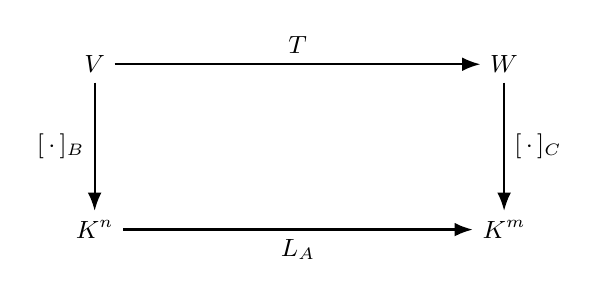
\begin{tikzpicture}[>=Latex,every node/.style={font=\small}]
 \node (V) at (0,2.1) {\(V\)};
 \node (W) at (5.2,2.1) {\(W\)};
 \node (Kn) at (0,0) {\(K^n\)};
 \node (Km) at (5.2,0) {\(K^m\)};
 \draw[->,thick] (V)--node[above]{\(T\)}(W);
 \draw[->,thick] (V)--node[left]{\([\,\cdot\,]_B\)}(Kn);
 \draw[->,thick] (W)--node[right]{\([\,\cdot\,]_C\)}(Km);
 \draw[->,thick] (Kn)--node[below]{\(L_A\)}(Km);
\end{tikzpicture}
\caption{Diagram współrzędnych dla
\(A=[T]_{C\leftarrow B}\).
Obie drogi z \(V\) do \(K^m\) dają tę samą kolumnę:
\([T(v)]_C=A[v]_B\).}
\label{fig:lin4-wspolrzedne}
\end{figure}

\begin{przyklad}[Macierz z obrazu wektorów bazowych]
\label{prz:lin4-macierz-z-obrazow}
Niech \(T\colon\mathbb R^3\to\mathbb R^2\)
będzie dane przez \(T(x,y,z)=(x+y,y+z)\),
tak jak w Przykładzie~\ref{prz:lin3-rzad-r3}.
Dla baz standardowych \(E_3\) i \(E_2\) mamy
\[
 T(e_1)=\begin{pmatrix}1\\0\end{pmatrix},
 \quad T(e_2)=\begin{pmatrix}1\\1\end{pmatrix},
 \quad T(e_3)=\begin{pmatrix}0\\1\end{pmatrix}.
\]
Ustawiając te kolumny w podanej kolejności,
otrzymujemy
\[
 [T]_{E_2\leftarrow E_3}
 =\begin{pmatrix}1&1&0\\0&1&1\end{pmatrix}.
\]
Obliczenie na kolumnie \((2,-1,3)^{\mathsf T}\)
z Przykładu~\ref{prz:lin4-iloczyn-kolumny}
daje \((1,2)^{\mathsf T}\), co zgadza się
z \(T(2,-1,3)=(1,2)\).
\end{przyklad}

\begin{twierdzenie}[Izomorfizm przestrzeni odwzorowań i macierzy]
\label{thm:lin4-hom-mat}
Niech \(V,W\) będą przestrzeniami wektorowymi
nad \(K\) o skończonych wymiarach odpowiednio
\(n,m\in\mathbb N_0\), a \(B,C\)
ich ustalonymi uporządkowanymi bazami.
Wtedy przyporządkowanie
\[
 \mathcal M_{C\leftarrow B}\colon
 \operatorname{Hom}_K(V,W)
 \longrightarrow\operatorname{Mat}_{m\times n}(K),
 \qquad T\longmapsto[T]_{C\leftarrow B}
\]
jest izomorfizmem przestrzeni wektorowych.
W szczególności
\(\dim_K\operatorname{Hom}_K(V,W)=mn\).
\end{twierdzenie}
\begin{proof}
Dla \(S,T\colon V\to W\) liniowych
oraz \(a,b\in K\), z równości
\((aS+bT)(b_j)=aS(b_j)+bT(b_j)\)
wynika, że każda kolumna macierzy
\([aS+bT]_{C\leftarrow B}\)
jest odpowiednią kombinacją kolumn
macierzy \(S\) i \(T\).
Zatem
\[
 [aS+bT]_{C\leftarrow B}
 =a[S]_{C\leftarrow B}
  +b[T]_{C\leftarrow B},
\]
co dowodzi liniowości \(\mathcal M_{C\leftarrow B}\).
Poprzednie twierdzenie zapewnia, że
każda macierz pochodzi od dokładnie jednego \(T\).
Odwzorowanie jest więc bijektywne.
Jako liniowa bijekcja jest izomorfizmem
na mocy Twierdzenia~\ref{thm:lin3-odwrotnosc}.
Równość wymiarów wynika z
Stwierdzenia~\ref{prop:lin4-przestrzen-macierzy}.
Dowód nie wymaga aksjomatu wyboru,
gdyż bazy \(B,C\) są już dane.
\end{proof}

\section{Mnożenie macierzy i składanie odwzorowań}
\label{sec:lin4-mnozenie}

\begin{definicja}[Iloczyn dwóch macierzy]
\label{def:lin4-iloczyn-macierzy}
Niech \(m,n,p\in\mathbb N_0\),
\(A=(a_{ij})\in\operatorname{Mat}_{m\times n}(K)\)
i \(B=(b_{jk})\in\operatorname{Mat}_{n\times p}(K)\).
\emph{Iloczynem} \(AB\) nazywamy macierz
w \(\operatorname{Mat}_{m\times p}(K)\)
o wyrazach
\[
 (AB)_{ik}=\sum_{j=1}^{n}a_{ij}b_{jk},
 \qquad 1\leq i\leq m,\quad 1\leq k\leq p.
\]
Wymiar wewnętrzny \(n\) musi być taki sam
dla obu macierzy. Iloczyn \(BA\) może
nie być określony.
\end{definicja}

\begin{twierdzenie}[Macierz złożenia]
\label{thm:lin4-macierz-zlozenia}
Niech \(U,V,W\) będą przestrzeniami
wektorowymi nad \(K\), o wymiarach
odpowiednio \(p,n,m\in\mathbb N_0\).
Niech \(D,B,C\) będą uporządkowanymi bazami
tych przestrzeni, a \(S\colon U\to V\),
\(T\colon V\to W\) odwzorowaniami liniowymi.
Wtedy
\[
 [T\circ S]_{C\leftarrow D}
 =[T]_{C\leftarrow B}\,[S]_{B\leftarrow D}.
\]
\end{twierdzenie}
\begin{proof}
Niech \(A=[T]_{C\leftarrow B}\),
\(M=[S]_{B\leftarrow D}\).
Dla dowolnego \(u\in U\)
dwukrotne zastosowanie
Twierdzenia~\ref{thm:lin4-wspolrzedne-macierz}
daje
\[
 [(T\circ S)(u)]_C
 =A[S(u)]_B
 =A(M[u]_D).
\]
Sprawdźmy, że \(A(Mx)=(AM)x\)
dla każdej kolumny \(x\in K^p\).
Jej \(i\)-ta współrzędna po lewej stronie
wynosi
\[
 \sum_{j=1}^{n}a_{ij}
   \left(\sum_{k=1}^{p}m_{jk}x_k\right)
 =\sum_{k=1}^{p}
   \left(\sum_{j=1}^{n}a_{ij}m_{jk}\right)x_k,
\]
co z definicji jest \(i\)-tą współrzędną
\((AM)x\). Przestawienie sum jest uprawnione,
ponieważ obie sumy są skończone.
Ostatecznie
\([(T\circ S)(u)]_C=(AM)[u]_D\).
Jednoznaczność macierzy odwzorowania
daje wzór z tezy.
\end{proof}

\begin{przyklad}[Mnożenie macierzy]
\label{prz:lin4-mnozenie}
Niech
\[
 A=\begin{pmatrix}1&2&0\\0&-1&3\end{pmatrix},
 \qquad
 B=\begin{pmatrix}1&0\\2&1\\0&-1\end{pmatrix}
\]
będą macierzami nad \(\mathbb R\),
odpowiednio o rozmiarach \(2\times3\)
i \(3\times2\). Wtedy
\[
 AB=
 \begin{pmatrix}
 1\cdot1+2\cdot2+0\cdot0&
 1\cdot0+2\cdot1+0\cdot(-1)\\
 0\cdot1+(-1)\cdot2+3\cdot0&
 0\cdot0+(-1)\cdot1+3\cdot(-1)
 \end{pmatrix}
 =\begin{pmatrix}5&2\\-2&-4\end{pmatrix}.
\]
Natomiast \(BA\) ma rozmiar \(3\times3\);
nie może więc być równe \(AB\)
nawet przed wykonaniem rachunków.
\end{przyklad}

\begin{definicja}[Macierz jednostkowa]
\label{def:lin4-jednostkowa}
Dla \(n\in\mathbb N_0\)
macierzą \emph{jednostkową} \(I_n\)
nazywamy macierz kwadratową
o wyrazach
\[
 (I_n)_{ij}=
 \begin{cases}
 1_K,&i=j,\\
 0_K,&i\neq j.
 \end{cases}
\]
Jej kolumny to wektory bazy standardowej \(K^n\).
Dla \(n=0\) jest to jedyna macierz \(0\times0\).
\end{definicja}

\begin{twierdzenie}[Łączność i rozdzielność iloczynu macierzy]
\label{thm:lin4-rachunek-macierzy}
Niech \(m,n,p,q\in\mathbb N_0\) oraz
\(A\in\operatorname{Mat}_{m\times n}(K)\),
\(B\in\operatorname{Mat}_{n\times p}(K)\),
\(C\in\operatorname{Mat}_{p\times q}(K)\).
Wtedy
\[
 (AB)C=A(BC).
\]
Ponadto dla dowolnych
\(A'\in\operatorname{Mat}_{m\times n}(K)\),
\(B'\in\operatorname{Mat}_{n\times p}(K)\)
i \(a\in K\) iloczyn jest rozdzielny
względem dodawania i zgodny z mnożeniem
przez skalar:
\[
 \begin{gathered}
 (A+A')B=AB+A'B,\qquad
 A(B+B')=AB+AB',\\
 (aA)B=a(AB)=A(aB).
 \end{gathered}
\]
Dla każdego \(D\in\operatorname{Mat}_{m\times n}(K)\)
zachodzi \(I_mD=D=DI_n\).
W przypadku macierzy kwadratowych
iloczyn na ogół nie jest przemienny.
\end{twierdzenie}
\begin{proof}
Wyraz \((i,\ell)\) macierzy \((AB)C\)
ma postać
\[
 \sum_{k=1}^{p}(AB)_{ik}c_{k\ell}
 =\sum_{k=1}^{p}\sum_{j=1}^{n}
    a_{ij}b_{jk}c_{k\ell}.
\]
W macierzy \(A(BC)\) ten sam wyraz
wynosi \(\sum_{j=1}^{n}\sum_{k=1}^{p}
a_{ij}b_{jk}c_{k\ell}\).
Równości są identyczne po przestawieniu
dwóch sum skończonych, co dowodzi łączności.

Dla przykładu wyraz \((i,k)\) iloczynu
\((A+A')B\) wynosi
\[
 \sum_{j=1}^{n}(a_{ij}+a'_{ij})b_{jk}
 =\sum_{j=1}^{n}a_{ij}b_{jk}
  +\sum_{j=1}^{n}a'_{ij}b_{jk}.
\]
Jest to wyraz macierzy \(AB+A'B\).
Pozostałe równości wynikają z tych samych aksjomatów ciała.
Dla macierzy \(A\) i \(B,B'\) odpowiednich rozmiarów
oraz skalara \(c\in K\) sprawdzamy ich współrzędne:
\[
 \begin{aligned}
 (A(B+B'))_{ik}&=\sum_j a_{ij}(b_{jk}+b'_{jk})
   =(AB)_{ik}+(AB')_{ik},\\
 ((cA)B)_{ik}&=\sum_j(ca_{ij})b_{jk}
   =c\sum_j a_{ij}b_{jk}=(c(AB))_{ik},\\
 (A(cB))_{ik}&=\sum_j a_{ij}(cb_{jk})
   =c\sum_j a_{ij}b_{jk}=(c(AB))_{ik}.
 \end{aligned}
\]
Każda suma jest skończona; wyciągnięcie skalara
przed sumę korzysta z rozdzielności w ciele \(K\).

Wyraz \((i,j)\) macierzy \(I_mD\)
jest równy
\(\sum_{k=1}^{m}(I_m)_{ik}d_{kj}=d_{ij}\),
ponieważ tylko składnik z \(k=i\)
może być niezerowy.
Podobnie \(DI_n=D\).
Jeśli któryś wymiar wynosi zero,
wszystkie odpowiednie równości dotyczą
jedynych macierzy rozmiaru z pustym
zbiorem indeksów albo sum pustych;
pozostają więc prawdziwe.

Nieprzemienność pokażemy już dla \(n=2\).
Niech
\[
 P=\begin{pmatrix}1&0\\0&0\end{pmatrix},
 \qquad
 Q=\begin{pmatrix}0&1\\1&0\end{pmatrix}.
\]
Wtedy
\[
 PQ=\begin{pmatrix}0&1\\0&0\end{pmatrix},
 \qquad
 QP=\begin{pmatrix}0&0\\1&0\end{pmatrix}.
\]
Macierze są różne nad każdym ciałem,
gdyż \(1_K\neq0_K\).
\end{proof}

\section{Jądro, obraz i rząd macierzy}
\label{sec:lin4-rzad-macierzy}

\begin{definicja}[Jądro, obraz i rząd macierzy]
\label{def:lin4-rzad-macierzy}
Niech \(m,n\in\mathbb N_0\) oraz
\(A\in\operatorname{Mat}_{m\times n}(K)\).
Definiujemy
\[
 \ker A:=\{x\in K^n:Ax=0_{K^m}\},\qquad
 \operatorname{im}A:=\{Ax:x\in K^n\},
\]
a \emph{rzędem macierzy} nazywamy liczbę
\[
 \operatorname{rk}A:=\dim_K(\operatorname{im}A).
\]
Są to odpowiednio jądro, obraz i rząd
odwzorowania \(L_A\colon K^n\to K^m\).
\end{definicja}

\begin{twierdzenie}[Kolumny, jądro i rząd]
\label{thm:lin4-rzad-kolumn}
Niech \(m,n\in\mathbb N_0\), a
\(A\in\operatorname{Mat}_{m\times n}(K)\)
ma kolumny \(a_1,\ldots,a_n\in K^m\).
Wtedy
\[
 \operatorname{im}A=\operatorname{span}\{a_1,\ldots,a_n\},
 \qquad
 \ker A=\left\{x\in K^n:
   \sum_{j=1}^{n}x_ja_j=0_{K^m}\right\}.
\]
W szczególności
\(\operatorname{rk}A\) jest wymiarem
przestrzeni rozpiętej przez kolumny,
a \(0\leq\operatorname{rk}A\leq\min\{m,n\}\).
Ponadto
\[
 n=\dim_K(\ker A)+\operatorname{rk}A.
\]
\end{twierdzenie}
\begin{proof}
Na mocy Stwierdzenia~\ref{prop:lin4-kolumny}
dla każdego \(x\in K^n\) zachodzi
\(Ax=\sum_{j=1}^{n}x_ja_j\).
Każdy element obrazu jest więc
kombinacją kolumn, a każda taka kombinacja
jest obrazem kolumny współczynników \(x\).
Dowodzi to pierwszej równości.
Druga jest definicją jądra po podstawieniu
tego samego wzoru.

Obraz jest podprzestrzenią \(K^m\),
zatem jego wymiar nie przekracza \(m\).
Jest też rozpięty przez \(n\) kolumn,
więc wymiar nie przekracza \(n\)
na mocy wyników o rodzinach rozpinających
z Rozdziału~\ref{ch:lin-przestrzenie-wektorowe}.
Twierdzenie~\ref{thm:lin3-rzad-nullity}
zastosowane do \(L_A\) daje
\(n=\dim_K\ker A+\operatorname{rk}A\).
Wszystkie wymiary są skończone.
\end{proof}

\begin{wniosek}[Kryteria iniektywności i surjektywności macierzy]
\label{cor:lin4-kryteria-kolumn}
Niech \(m,n\in\mathbb N_0\) oraz
\(A\in\operatorname{Mat}_{m\times n}(K)\).
Wtedy \(L_A\colon K^n\to K^m\) jest
iniektywne wtedy i tylko wtedy, gdy
kolumny \(A\) są liniowo niezależne.
Jest surjektywne wtedy i tylko wtedy,
gdy kolumny rozpinają \(K^m\).
\end{wniosek}
\begin{proof}
Z poprzedniego twierdzenia \(\ker A=\{0\}\)
dokładnie wtedy, gdy warunek
\(\sum_jx_ja_j=0\) wymusza \(x_j=0_K\)
dla wszystkich \(j\).
To definicja niezależności liniowej kolumn.
Surjektywność jest równoważna
\(\operatorname{im}A=K^m\),
czyli rozpinaniu przez kolumny.
\end{proof}

\begin{przyklad}[Rząd prostokątnej macierzy]
\label{prz:lin4-rzad-prostokatnej}
Dla
\[
 A=\begin{pmatrix}1&1&0\\0&1&1\end{pmatrix}
\]
nad \(\mathbb R\) pierwsza i trzecia kolumna
to \((1,0)^{\mathsf T}\) i \((0,1)^{\mathsf T}\).
Tworzą bazę \(\mathbb R^2\), zatem
\(\operatorname{im}A=\mathbb R^2\)
i \(\operatorname{rk}A=2\).
Układ \(Ax=0\) daje
\(x_1+x_2=0,\ x_2+x_3=0\), więc
\[
 \ker A=\operatorname{span}\{
 (-1,1,-1)^{\mathsf T}\}.
\]
Wymiar jądra wynosi \(1\), zgodnie z
\(3=1+2\).
\end{przyklad}

\section{Macierze odwracalne}
\label{sec:lin4-odwracalne}

\begin{definicja}[Macierz odwracalna]
\label{def:lin4-odwracalna}
Niech \(n\in\mathbb N_0\).
Macierz \(A\in\operatorname{Mat}_{n\times n}(K)\)
nazywamy \emph{odwracalną}, gdy istnieje
\(B\in\operatorname{Mat}_{n\times n}(K)\)
taka, że \(AB=I_n=BA\).
Macierz \(B\), jeśli istnieje, nazywamy
\emph{odwrotną} do \(A\) i oznaczamy \(A^{-1}\).
\end{definicja}

\begin{twierdzenie}[Kryteria odwracalności]
\label{thm:lin4-odwracalnosc-kryteria}
Niech \(n\in\mathbb N_0\) oraz
\(A\in\operatorname{Mat}_{n\times n}(K)\).
Następujące warunki są równoważne:
\begin{enumerate}[label=(\roman*)]
\item \(A\) jest odwracalna;
\item \(L_A\colon K^n\to K^n\) jest bijektywne;
\item kolumny \(A\) tworzą bazę \(K^n\);
\item \(\ker A=\{0_{K^n}\}\);
\item \(\operatorname{im}A=K^n\).
\end{enumerate}
Gdy zachodzą, macierz odwrotna jest jednoznaczna
i spełnia
\[
 [L_A^{-1}]_{E_n\leftarrow E_n}=A^{-1}.
\]
\end{twierdzenie}
\begin{proof}
Jeśli \(AB=I_n=BA\), to
z Twierdzenia~\ref{thm:lin4-macierz-zlozenia}
otrzymujemy
\(L_A\circ L_B=\operatorname{id}_{K^n}
 =L_B\circ L_A\).
Odwzorowanie \(L_A\) jest zatem bijektywne.

Jeśli \(L_A\) jest bijektywne,
jego odwrotność jest liniowa na mocy
Twierdzenia~\ref{thm:lin3-odwrotnosc}.
Niech \(B\) będzie macierzą \(L_A^{-1}\)
w bazie standardowej.
Wzór na macierz złożenia daje
\(AB=I_n=BA\). Stąd (i) i (ii)
są równoważne.

Kolumny \(A\) są obrazami bazy standardowej
przez \(L_A\). Na mocy
Stwierdzenia~\ref{prop:lin3-izomorfizm-baza}
bijektywność \(L_A\) implikuje, że kolumny
tworzą bazę. Odwrotnie, gdy kolumny
tworzą bazę, są niezależne i rozpinające,
więc zgodnie z Wnioskiem~\ref{cor:lin4-kryteria-kolumn}
odwzorowanie \(L_A\) jest zarówno iniektywne,
jak i surjektywne. Otrzymaliśmy (ii)
równoważne (iii).

Na mocy Wniosku~\ref{cor:lin3-rownymiary}
dla endomorfizmu skończenie wymiarowej
przestrzeni \(K^n\) iniektywność,
surjektywność i bijektywność są równoważne.
Twierdzenie~\ref{thm:lin3-iniekcja-surjekcja}
utożsamia iniektywność z (iv),
a surjektywność z (v).
Wszystkie warunki są zatem równoważne.

Jeżeli \(B,C\) są dwiema macierzami odwrotnymi
do \(A\), to z łączności mnożenia
\[
 B=B(AC)=(BA)C=I_nC=C.
\]
To dowodzi jednoznaczności.
Przy \(n=0\) wszystkie warunki zachodzą
dla jedynej macierzy \(0\times0\),
a wzory pozostają poprawne.
\end{proof}

\begin{przyklad}[Odwrotność macierzy o rozmiarze \(2\times2\)]
\label{prz:lin4-odwrotnosc-2}
Nad \(\mathbb R\) niech
\[
 A=\begin{pmatrix}2&1\\1&1\end{pmatrix},
 \qquad
 B=\begin{pmatrix}1&-1\\-1&2\end{pmatrix}.
\]
Mnożenie daje
\[
 AB=
 \begin{pmatrix}
 2\cdot1+1\cdot(-1)&2\cdot(-1)+1\cdot2\\
 1\cdot1+1\cdot(-1)&1\cdot(-1)+1\cdot2
 \end{pmatrix}
 =I_2.
\]
Dla iloczynu w odwrotnej kolejności obliczamy również
\[
 BA=\begin{pmatrix}
 1\cdot2+(-1)\cdot1&1\cdot1+(-1)\cdot1\\
 (-1)\cdot2+2\cdot1&(-1)\cdot1+2\cdot1
 \end{pmatrix}=I_2.
\]
Zatem \(A^{-1}=B\).
Nie skorzystaliśmy jeszcze z wyznaczników;
wystarczy sprawdzić oba iloczyny.
\end{przyklad}

\begin{stwierdzenie}[Iloczyn i odwrotność macierzy odwracalnych]
\label{prop:lin4-iloczyn-odwrotnych}
Niech \(n\in\mathbb N_0\), a
\(A,B\in\operatorname{Mat}_{n\times n}(K)\)
będą odwracalne. Wtedy \(AB\) jest odwracalna
oraz
\[
 (AB)^{-1}=B^{-1}A^{-1},\qquad
 (A^{-1})^{-1}=A.
\]
\end{stwierdzenie}
\begin{proof}
Korzystając z łączności mnożenia,
\[
 (AB)(B^{-1}A^{-1})
 =A(BB^{-1})A^{-1}=AA^{-1}=I_n.
\]
Podobnie
\((B^{-1}A^{-1})(AB)
 =B^{-1}(A^{-1}A)B=I_n\).
Jednoznaczność odwrotności daje pierwszy wzór.
Równości \(AA^{-1}=I_n=A^{-1}A\)
dowodzą, że \(A\) jest odwrotnością \(A^{-1}\),
czyli drugiego wzoru.
\end{proof}

\section{Macierze zmiany bazy}
\label{sec:lin4-zmiana-bazy}

\begin{definicja}[Macierz przejścia między bazami]
\label{def:lin4-przejscie}
Niech \(n\in\mathbb N_0\), a \(V\)
będzie \(n\)-wymiarową przestrzenią
wektorową nad \(K\). Niech
\(B=(b_1,\ldots,b_n)\) i
\(B'=(b'_1,\ldots,b'_n)\) jej uporządkowanymi bazami.
\emph{Macierzą przejścia od współrzędnych w \(B'\)
do współrzędnych w \(B\)} nazywamy
\[
 P_{B\leftarrow B'}
 :=\bigl([b'_1]_B\ \cdots\ [b'_n]_B\bigr)
 \in\operatorname{Mat}_{n\times n}(K).
\]
Jej \(j\)-ta kolumna zawiera współrzędne
\(j\)-tego wektora nowej bazy \(B'\)
w starej bazie \(B\).
\end{definicja}

\begin{twierdzenie}[Współrzędne przy zmianie bazy]
\label{thm:lin4-zmiana-wspolrzednych}
Niech \(V\) będzie przestrzenią wektorową
nad \(K\) o wymiarze \(n\in\mathbb N_0\),
a \(B=(b_1,\ldots,b_n)\) i
\(B'=(b'_1,\ldots,b'_n)\) jej
uporządkowanymi bazami.
Macierz \(P:=P_{B\leftarrow B'}\)
jest odwracalna i dla każdego \(v\in V\)
zachodzi
\[
 [v]_B=P[v]_{B'},\qquad
 [v]_{B'}=P^{-1}[v]_B.
\]
Ponadto
\[
 P_{B'\leftarrow B}=P_{B\leftarrow B'}^{-1}.
\]
\end{twierdzenie}
\begin{proof}
Rozważmy odwzorowanie identycznościowe
\(\operatorname{id}_V\colon V\to V\).
Z definicji jego macierz w bazach
wejściowej \(B'\) i wyjściowej \(B\)
ma w \(j\)-tej kolumnie \([b'_j]_B\),
a więc jest równa \(P\).
Twierdzenie~\ref{thm:lin4-wspolrzedne-macierz}
daje
\([v]_B=P[v]_{B'}\) dla każdego \(v\in V\).

Podobnie \(Q:=P_{B'\leftarrow B}\)
spełnia \([v]_{B'}=Q[v]_B\).
Po podstawieniu pierwszej równości
otrzymujemy
\([v]_{B'}=QP[v]_{B'}\).
Ponieważ odwzorowanie współrzędnych
\(V\to K^n\) jest surjektywne,
mamy \(QP x=x\) dla każdego \(x\in K^n\),
co daje \(QP=I_n\).
W odwrotnej kolejności podstawień
otrzymujemy \(PQ=I_n\).
Zatem \(P\) jest odwracalna i \(Q=P^{-1}\).
Wszystko pozostaje poprawne przy \(n=0\).
\end{proof}

\begin{przyklad}[Współrzędne w dwóch bazach]
\label{prz:lin4-zmiana-wspolrzednych}
Niech \(V=\mathbb R^2\),
\(B=((1,0),(0,1))\) oraz
\(B'=((1,1),(0,1))\).
Wtedy
\[
 P_{B\leftarrow B'}
 =\begin{pmatrix}1&0\\1&1\end{pmatrix},
 \qquad
 P_{B\leftarrow B'}^{-1}
 =\begin{pmatrix}1&0\\-1&1\end{pmatrix}.
\]
Dla wektora \(v=(2,3)\) mamy
\([v]_B=(2,3)^{\mathsf T}\),
a zatem
\[
 [v]_{B'}=
 \begin{pmatrix}1&0\\-1&1\end{pmatrix}
 \begin{pmatrix}2\\3\end{pmatrix}
 =\begin{pmatrix}2\\1\end{pmatrix}.
\]
Istotnie, \((2,3)=2(1,1)+(0,1)\).
Nie zmieniliśmy wektora \(v\), tylko
jego współrzędne.
\end{przyklad}

\begin{twierdzenie}[Zmiana baz dziedziny i przeciwdziedziny]
\label{thm:lin4-zmiana-macierzy}
Niech \(V,W\) będą przestrzeniami wektorowymi
nad \(K\), o wymiarach \(n,m\in\mathbb N_0\),
a \(T\colon V\to W\) odwzorowaniem liniowym.
Niech \(B,B'\) będą uporządkowanymi bazami \(V\),
a \(C,C'\) uporządkowanymi bazami \(W\).
Oznaczmy
\[
 A=[T]_{C\leftarrow B},\qquad
 P=P_{B\leftarrow B'},\qquad
 Q=P_{C\leftarrow C'}.
\]
Wówczas
\[
 [T]_{C'\leftarrow B'}=Q^{-1}AP.
\]
\end{twierdzenie}
\begin{proof}
Dla dowolnego \(v\in V\) mamy
\([v]_B=P[v]_{B'}\) na mocy
Twierdzenia~\ref{thm:lin4-zmiana-wspolrzednych}.
Ponadto
\([T(v)]_C=A[v]_B\).
W przypadku przestrzeni \(W\)
to samo twierdzenie daje
\([T(v)]_{C'}=Q^{-1}[T(v)]_C\).
Łącząc te równości, otrzymujemy
\[
 [T(v)]_{C'}=Q^{-1}AP[v]_{B'}.
\]
Macierz \(Q^{-1}AP\) ma rozmiar \(m\times n\).
Jednoznaczność macierzy odwzorowania
z Twierdzenia~\ref{thm:lin4-wspolrzedne-macierz}
daje tezę.
\end{proof}

\begin{wniosek}[Macierze podobne]
\label{cor:lin4-podobienstwo}
Niech \(V\) będzie skończenie wymiarową
przestrzenią wektorową nad \(K\),
\(T\colon V\to V\) endomorfizmem,
a \(B,B'\) dwiema uporządkowanymi bazami \(V\).
Dla \(A=[T]_{B\leftarrow B}\) i
\(P=P_{B\leftarrow B'}\) zachodzi
\[
 [T]_{B'\leftarrow B'}=P^{-1}AP.
\]
Dwie macierze kwadratowe \(A,A'\)
tego samego rozmiaru nazywamy
\emph{podobnymi}, gdy istnieje
odwracalna macierz \(P\) taka, że
\(A'=P^{-1}AP\).
\end{wniosek}
\begin{proof}
W Twierdzeniu~\ref{thm:lin4-zmiana-macierzy}
wybieramy \(W=V\), \(C=B\), \(C'=B'\).
Wtedy obie macierze przejścia są równe \(P\),
co daje wzór z tezy.
\end{proof}

\begin{przyklad}[Zmiana macierzy endomorfizmu]
\label{prz:lin4-podobienstwo}
W \(\mathbb R^2\) rozważmy
\(T(x,y)=(2x+y,y)\).
Dla bazy standardowej \(B\) mamy
\[
 A=[T]_{B\leftarrow B}
 =\begin{pmatrix}2&1\\0&1\end{pmatrix}.
\]
Niech \(B'=((1,1),(0,1))\), jak w
Przykładzie~\ref{prz:lin4-zmiana-wspolrzednych}.
Wówczas
\[
 P=\begin{pmatrix}1&0\\1&1\end{pmatrix},
 \qquad
 P^{-1}AP
 =\begin{pmatrix}1&0\\-1&1\end{pmatrix}
  \begin{pmatrix}2&1\\0&1\end{pmatrix}
  \begin{pmatrix}1&0\\1&1\end{pmatrix}
 =\begin{pmatrix}3&1\\-2&0\end{pmatrix}.
\]
Możemy to sprawdzić bezpośrednio:
\(T(1,1)=(3,1)=3(1,1)-2(0,1)\),
a \(T(0,1)=(1,1)=1(1,1)+0(0,1)\).
Nowa macierz ma więc kolumny
\((3,-2)^{\mathsf T}\) i \((1,0)^{\mathsf T}\).
\end{przyklad}

\begin{uwaga}[Co jest niezmiennicze przy zmianie bazy?]
\label{rem:lin4-niezmienniki}
Macierz odwzorowania zależy od wyboru
uporządkowanych baz, ale samo odwzorowanie
nie ulega zmianie. Jądro i obraz mają
niezależnie od baz te same wymiary:
przejścia \(P,Q\) są odwracalne,
zatem \(x\mapsto Px\) daje bijekcję
między rozwiązaniami \(Q^{-1}APx=0\)
a rozwiązaniami \(Ay=0\).
Podobnie obraz nowej macierzy
jest obrazem starej przez izomorfizm \(Q^{-1}\).
W szczególności rząd nie zmienia się
przy zmianie baz.
\end{uwaga}

\section{Transpozycja macierzy}
\label{sec:lin4-transpozycja}

\begin{definicja}[Macierz transponowana]
\label{def:lin4-transpozycja}
Niech \(m,n\in\mathbb N_0\).
Dla \(A=(a_{ij})\in\operatorname{Mat}_{m\times n}(K)\)
przez \emph{macierz transponowaną} rozumiemy
\[
 A^{\mathsf T}:=(a_{ji})_{1\leq j\leq n,\ 1\leq i\leq m}
 \in\operatorname{Mat}_{n\times m}(K).
\]
Transpozycja zamienia wiersze z kolumnami;
nie wykonuje sprzężenia zespolonego.
\end{definicja}

\begin{stwierdzenie}[Działania i transpozycja]
\label{prop:lin4-transpozycja-dzialania}
Niech \(m,n,p\in\mathbb N_0\),
\(A,B\in\operatorname{Mat}_{m\times n}(K)\)
oraz \(c\in K\). Wtedy
\[
 (A+B)^{\mathsf T}=A^{\mathsf T}+B^{\mathsf T},
 \quad(cA)^{\mathsf T}=cA^{\mathsf T},
 \quad(A^{\mathsf T})^{\mathsf T}=A.
\]
Ponadto dla \(A\in\operatorname{Mat}_{m\times n}(K)\)
i \(D\in\operatorname{Mat}_{n\times p}(K)\)
zachodzi
\[
 (AD)^{\mathsf T}=D^{\mathsf T}A^{\mathsf T}.
\]
\end{stwierdzenie}
\begin{proof}
Pierwsze trzy równości wynikają
z porównania odpowiednich wyrazów:
na przykład wyraz \((j,i)\) macierzy
\((A+B)^{\mathsf T}\) wynosi
\(a_{ij}+b_{ij}\), tak samo jak
w macierzy \(A^{\mathsf T}+B^{\mathsf T}\).

Dla ostatniego wzoru wyraz \((k,i)\)
macierzy \((AD)^{\mathsf T}\) jest równy
\[
 (AD)_{ik}=\sum_{j=1}^{n}a_{ij}d_{jk}.
\]
W macierzy \(D^{\mathsf T}A^{\mathsf T}\)
wyraz o tych samych indeksach wynosi
\(\sum_{j=1}^{n}(D^{\mathsf T})_{kj}
(A^{\mathsf T})_{ji}
=\sum_{j=1}^{n}d_{jk}a_{ij}\).
Obie wartości są równe, bo mnożenie
w ciele \(K\) jest przemienne.
Także przy pustych zbiorach indeksów
sumy i macierze są zgodne.
\end{proof}

\begin{przyklad}[Transpozycja iloczynu]
\label{prz:lin4-transpozycja}
Niech
\[
 A=\begin{pmatrix}1&2\\0&-1\end{pmatrix},
 \qquad
 D=\begin{pmatrix}2\\3\end{pmatrix}
\]
nad \(\mathbb R\).
Mamy
\(AD=(8,-3)^{\mathsf T}\), więc
\((AD)^{\mathsf T}=(8,-3)\).
Z drugiej strony
\[
 D^{\mathsf T}A^{\mathsf T}
 =\begin{pmatrix}2&3\end{pmatrix}
  \begin{pmatrix}1&0\\2&-1\end{pmatrix}
 =\begin{pmatrix}8&-3\end{pmatrix}.
\]
Przykład potwierdza odwrócenie
kolejności czynników w transpozycji iloczynu.
\end{przyklad}

\section{Układ równań liniowych jako równanie macierzowe}
\label{sec:lin4-uklady}

\begin{definicja}[Układ liniowy w postaci macierzowej]
\label{def:lin4-uklad}
Niech \(m,n\in\mathbb N_0\),
\(A=(a_{ij})\in\operatorname{Mat}_{m\times n}(K)\),
a \(b=(b_1,\ldots,b_m)^{\mathsf T}\in K^m\).
Równanie macierzowe \(Ax=b\), \(x\in K^n\),
oznacza układ \(m\) równań
\[
 \sum_{j=1}^{n}a_{ij}x_j=b_i,
 \qquad 1\leq i\leq m.
\]
Układ \(Ax=0_{K^m}\) nazywamy
\emph{jednorodnym}; inne układy nazywamy
\emph{niejednorodnymi}.
\end{definicja}

\begin{twierdzenie}[Warunek rozwiązalności i wszystkie rozwiązania]
\label{thm:lin4-zbior-rozwiazan}
Niech \(A\in\operatorname{Mat}_{m\times n}(K)\)
oraz \(b\in K^m\), gdzie \(m,n\in\mathbb N_0\).
Układ \(Ax=b\) ma rozwiązanie
wtedy i tylko wtedy, gdy \(b\in\operatorname{im}A\).
Jeżeli \(x_0\in K^n\) jest jednym rozwiązaniem,
to zbiór wszystkich rozwiązań jest równy
\[
 x_0+\ker A=\{x_0+z:z\in\ker A\}.
\]
W szczególności układ jednorodny
ma zawsze rozwiązanie zerowe.
\end{twierdzenie}
\begin{proof}
Definicja obrazu mówi, że
\(b\in\operatorname{im}A\) dokładnie wtedy,
gdy istnieje \(x_0\in K^n\) z \(Ax_0=b\).
To dowodzi pierwszej równoważności.

Załóżmy teraz \(Ax_0=b\).
Dla \(x\in K^n\) mamy
\[
 Ax=b
 \iff Ax=Ax_0
 \iff A(x-x_0)=0_{K^m}
 \iff x-x_0\in\ker A.
\]
Wykorzystaliśmy liniowość \(L_A\).
Ostatni warunek jest równoważny
istnieniu \(z\in\ker A\)
takiego, że \(x=x_0+z\).
Daje to dokładnie wskazany zbiór rozwiązań.
Przy \(b=0_{K^m}\) można wziąć \(x_0=0_{K^n}\).
\end{proof}

\begin{przyklad}[Jawne rozwiązanie układu z parametrem]
\label{prz:lin4-rozwiazania-ukladu}
Niech
\[
 A=\begin{pmatrix}1&1&0\\0&1&1\end{pmatrix},
 \qquad b=\begin{pmatrix}\alpha\\\beta\end{pmatrix},
 \quad \alpha,\beta\in\mathbb R.
\]
Układ \(Ax=b\) ma postać
\(x_1+x_2=\alpha\), \(x_2+x_3=\beta\).
Jeżeli oznaczymy \(x_2=t\in\mathbb R\),
otrzymamy
\[
 \begin{pmatrix}x_1\\x_2\\x_3\end{pmatrix}
 =\begin{pmatrix}\alpha\\0\\\beta\end{pmatrix}
 +t\begin{pmatrix}-1\\1\\-1\end{pmatrix}.
\]
Każda wartość \(t\) daje rozwiązanie,
a każde rozwiązanie ma tę postać.
Pierwszy składnik jest rozwiązaniem
szczególnym, drugi przebiega \(\ker A\)
z Przykładu~\ref{prz:lin4-rzad-prostokatnej}.
Dla każdego \(b\) układ jest rozwiązalny,
ponieważ \(\operatorname{im}A=\mathbb R^2\).
\end{przyklad}

\section{Podsumowanie}
\label{sec:lin4-podsumowanie}

Macierz odwzorowania liniowego ma w kolumnach
współrzędne obrazów wektorów bazy dziedziny.
Wzór \([T(v)]_C=[T]_{C\leftarrow B}[v]_B\)
pozwala zastąpić działanie odwzorowania
mnożeniem macierzy przez kolumnę.
Mnożenie macierzy opisuje składanie odwzorowań,
a odwracalność macierzy jest równoważna
odwracalności odpowiedniego operatora.
Przy zmianie baz macierz \(A\) zmienia się
zgodnie ze wzorem \(Q^{-1}AP\);
dla endomorfizmu jest to podobieństwo
\(P^{-1}AP\).
Rząd macierzy jest wymiarem przestrzeni
rozpiętej przez jej kolumny, a rozwiązania
układu \(Ax=b\), gdy istnieją, tworzą warstwę
\(x_0+\ker A\).

\chapter{Eliminacja Gaussa i układy równań liniowych}
\label{ch:lin5-eliminacja-gaussa}
\index{eliminacja Gaussa@Eliminacja Gaussa}
\index{operacje elementarne@Operacje elementarne na wierszach}
\index{postac schodkowa@Postać schodkowa macierzy}

\noindent\textbf{Cel rozdziału.}
W Rozdziale~\ref{ch:lin4-macierze-zmiana-bazy}
opisaliśmy układy liniowe przez równania \(Ax=b\),
ich rozwiązania i rząd macierzy.
Obecnie przedstawimy skończony algorytm, który
pozwala obliczać rząd, rozstrzygać rozwiązalność,
wyznaczać wszystkie rozwiązania oraz znajdować
bazy jądra i obrazu. Wyprowadzimy go z operacji
na wierszach i udowodnimy poprawność, zamiast
traktować przekształcenia macierzy jako przepisy
rachunkowe bez uzasadnienia.

W całym rozdziale \(K\) jest ciałem z \(0_K\ne1_K\).
Wszystkie macierze i przestrzenie są nad \(K\),
a \(m,n\in\mathbb N_0\), o ile nie wskazano inaczej.
Nie zakładamy uporządkowania ciała ani możliwości
dzielenia przez zero. Przypadki pustych macierzy
interpretujemy zgodnie z
Definicją~\ref{def:lin4-macierz}.

\section{Elementarne operacje na wierszach}
\label{sec:lin5-operacje-wierszowe}

\begin{definicja}[Trzy typy operacji elementarnych]
\label{def:lin5-operacje}
Niech \(m,n\in\mathbb N_0\) i
\(A\in\operatorname{Mat}_{m\times n}(K)\).
\emph{Elementarną operacją na wierszach} nazywamy
jedno z następujących przekształceń:
\begin{enumerate}[label=(\roman*)]
\item zamianę miejscami dwóch różnych wierszy
\(R_i\leftrightarrow R_j\), \(i\ne j\);
\item pomnożenie wiersza \(R_i\) przez skalar
\(\lambda\in K\setminus\{0_K\}\),
czyli \(R_i\leftarrow\lambda R_i\);
\item dodanie do \(R_i\) wielokrotności innego wiersza,
czyli \(R_i\leftarrow R_i+\lambda R_j\), gdzie
\(i\ne j\) i \(\lambda\in K\).
\end{enumerate}
W każdym przypadku indeksy wierszy należą do
\(\{1,\ldots,m\}\). Dla \(m=0\) nie ma
żadnej operacji do wykonania.
Dwie macierze tego samego rozmiaru nazywamy
\emph{wierszowo równoważnymi}, gdy jedną można
otrzymać z drugiej przez skończony ciąg
operacji elementarnych, także ciąg pusty.
\end{definicja}

\begin{stwierdzenie}[Odwracalność operacji elementarnych]
\label{prop:lin5-odwracalne-operacje}
Niech \(m,n\in\mathbb N_0\) i
\(A\in\operatorname{Mat}_{m\times n}(K)\).
Każda operacja elementarna ma operację odwrotną
tego samego typu. Istnieje ponadto
odwracalna macierz \(E\in\operatorname{Mat}_{m\times m}(K)\)
taka, że wynik operacji na \(A\) jest równy \(EA\).
Dla dowolnych wierszowo równoważnych macierzy
\(A,B\in\operatorname{Mat}_{m\times n}(K)\)
istnieje odwracalna macierz
\(P\in\operatorname{Mat}_{m\times m}(K)\)
spełniająca \(B=PA\).
\end{stwierdzenie}
\begin{proof}
Zamiana wierszy odwraca się przez tę samą zamianę.
Mnożenie przez \(\lambda\ne0_K\) odwraca się
mnożeniem przez \(\lambda^{-1}\), a dodanie
\(\lambda R_j\) do \(R_i\) odwraca się dodaniem
\(-\lambda R_j\). Warunek \(i\ne j\) zapewnia,
że w ostatnim przypadku wiersz \(R_j\)
pozostaje niezmieniony.

Niech \(E\) powstaje z \(I_m\) przez tę
samą operację. Z definicji mnożenia macierzy
\(i\)-ty wiersz \(EA\) jest kombinacją wierszy
\(A\) o współczynnikach z \(i\)-tego wiersza \(E\).
Dlatego \(EA\) jest wynikiem żądanej operacji.
Macierz odpowiadająca operacji odwrotnej
jest dwustronną odwrotnością \(E\), gdyż
obie operacje zastosowane kolejno do \(I_m\)
dają \(I_m\). Zatem \(E\) jest odwracalna
na mocy Definicji~\ref{def:lin4-odwracalna}.

Dla ciągu operacji odpowiadających macierzom
\(E_1,\ldots,E_s\) otrzymujemy
\(B=E_s\cdots E_1 A\).
Iloczyn \(P=E_s\cdots E_1\) jest odwracalny
na mocy Stwierdzenia~\ref{prop:lin4-iloczyn-odwrotnych}.
Przy pustym ciągu bierzemy \(P=I_m\).
Rachunek działa również dla pustych rozmiarów.
\end{proof}

\begin{wniosek}[Równoważne układy liniowe]
\label{cor:lin5-rownowazne-uklady}
Niech \(A\in\operatorname{Mat}_{m\times n}(K)\),
\(b\in K^m\), a \(P\) będzie odwracalną
macierzą rozmiaru \(m\times m\).
Wtedy układy \(Ax=b\) i \(PAx=Pb\)
mają dokładnie ten sam zbiór rozwiązań.
W szczególności można wykonywać te same
operacje elementarne na wierszach macierzy
\(A\) i odpowiednich wyrazach kolumny \(b\).
\end{wniosek}
\begin{proof}
Dla każdego \(x\in K^n\) z \(Ax=b\)
po pomnożeniu przez \(P\) otrzymujemy
\(PAx=Pb\). Odwrotnie, pomnożenie
\(PAx=Pb\) przez \(P^{-1}\) daje \(Ax=b\).
Taką samą operację na \(A\) i \(b\)
realizuje mnożenie \([A\mid b]\) przez
macierz elementarną z lewej strony.
\end{proof}

\begin{uwaga}[Czego nie zachowują operacje wierszowe?]
\label{rem:lin5-obraz-wiersze}
Jeżeli \(B=PA\) i \(P\) jest odwracalna,
to \(\ker B=\ker A\), a
\(\operatorname{im}B=P(\operatorname{im}A)\).
W szczególności \(\operatorname{rk}B=\operatorname{rk}A\),
ale obrazy \(A\) i \(B\) nie muszą być
identycznymi podprzestrzeniami \(K^m\).
Na przykład dla
\(A=(1,0)^{\mathsf T}\) i \(B=(0,1)^{\mathsf T}\)
zamiana wierszy zachowuje rząd \(1\),
lecz zmienia obraz.
\end{uwaga}

\section{Postać schodkowa i algorytm eliminacji}
\label{sec:lin5-postac-schodkowa}

\begin{definicja}[Postać schodkowa]
\label{def:lin5-schodkowa}
Niech \(R\in\operatorname{Mat}_{m\times n}(K)\).
\emph{Pierwszym niezerowym wyrazem}
niezerowego wiersza nazywamy jego wyraz
o najmniejszym indeksie kolumny, w której
występuje skalar różny od \(0_K\).
Macierz \(R\) jest w \emph{postaci schodkowej},
gdy:
\begin{enumerate}[label=(\roman*)]
\item wszystkie wiersze zerowe leżą poniżej niezerowych;
\item indeksy kolumn pierwszych niezerowych wyrazów
kolejnych niezerowych wierszy ściśle rosną.
\end{enumerate}
Pierwsze niezerowe wyrazy nazywamy
\emph{elementami wiodącymi}, a ich kolumny
\emph{kolumnami bazowymi} (kolumnami z pivotem).
Postać schodkowa jest \emph{zredukowana},
gdy dodatkowo każdy element wiodący jest
równy \(1_K\) i stanowi jedyny niezerowy wyraz
w swojej kolumnie.
Dla \(m=0\) lub \(n=0\) jedyna macierz
ma postać schodkową zredukowaną.
\end{definicja}

\begin{twierdzenie}[Istnienie postaci schodkowej i zredukowanej]
\label{thm:lin5-gauss}
Dla dowolnych \(m,n\in\mathbb N_0\)
i \(A\in\operatorname{Mat}_{m\times n}(K)\)
istnieją wierszowo równoważne z \(A\)
macierze \(U,R\) tego samego rozmiaru,
z których \(U\) jest schodkowa,
a \(R\) schodkowa zredukowana.
Można je otrzymać skończoną liczbą
elementarnych operacji na wierszach.
\end{twierdzenie}
\begin{proof}
Podamy algorytm wraz z uzasadnieniem.
Ustawiamy numer aktualnego wiersza \(r=1\)
i przeglądamy kolumny \(j=1,\ldots,n\)
w rosnącej kolejności. Jeżeli \(r>m\),
kończymy; dalsze kolumny nie mogą
dostarczyć nowych wierszy niezerowych.

W rozpatrywanej kolumnie \(j\) szukamy
wiersza \(k\geq r\) z niezerowym wyrazem
w tej kolumnie. Gdy takiego wiersza nie ma,
przechodzimy do następnej kolumny.
Gdy istnieje, zamieniamy wiersze \(k\) i \(r\)
(jeżeli \(k=r\), zamiana nie jest potrzebna).
Element \(a_{rj}\) jest teraz niezerowy,
więc wolno pomnożyć wiersz \(r\)
przez \(a_{rj}^{-1}\), uzyskując jedynkę.
Od każdego wiersza \(i>r\) odejmujemy
\(a_{ij}\) razy nowy wiersz \(r\);
zerujemy zatem wszystkie wyrazy pod pivotem.
Zwiększamy \(r\) o \(1\).

Po wybraniu pivotu w kolumnie \(j\)
wszystkie wiersze poniżej \(r\) mają zera
w kolumnach wcześniej wybranych:
były tam wyzerowane podczas poprzednich
etapów, a kombinacje tych wierszy
nie wprowadzają nowych niezerowych wyrazów.
Jeżeli pewną kolumnę pominięto z powodu
samych zer pod aktualnym wierszem,
kolejne operacje na tych niższych wierszach
również zachowują w tej kolumnie zera.
Stąd kolejne wybrane pivoty występują
w ściśle rosnących kolumnach,
a wiersze niewybrane, jeśli pozostały,
są zerowe. Otrzymana macierz \(U\)
ma postać schodkową. Algorytm przegląda
dokładnie \(n\) kolumn i wybiera nie więcej
niż \(\min\{m,n\}\) pivotów, zatem się kończy.

Aby uzyskać postać zredukowaną, przechodzimy
po pivotach od ostatniego ku pierwszemu.
W każdym wierszu wiodący wyraz wynosi już \(1_K\).
Za jego pomocą odejmujemy odpowiednie
wielokrotności tego wiersza od wszystkich
wierszy położonych wyżej, zerując wyrazy
nad pivotem. Ponieważ wiersz z późniejszym
pivotem ma zera we wszystkich wcześniejszych
kolumnach bazowych, operacje te nie niszczą
zer uzyskanych w poprzednich krokach
ani samych jedynek wiodących.
Po zakończeniu każda kolumna bazowa ma
jedną jedynkę i same zera. Powstała
macierz \(R\) jest schodkowa zredukowana
i wierszowo równoważna z \(A\).

Jeżeli jeden z rozmiarów jest zerowy,
nie wykonujemy żadnego kroku;
jedyna macierz już jest zredukowana.
\end{proof}

\begin{przyklad}[Dwa etapy eliminacji]
\label{prz:lin5-pierwsza-eliminacja}
Nad \(\mathbb R\) niech
\[
 A=\begin{pmatrix}
 1&2&1&0\\
 2&4&3&1\\
 1&2&2&1
 \end{pmatrix}.
\]
Odejmujemy dwukrotność pierwszego wiersza
od drugiego i pierwszy wiersz od trzeciego:
\[
 A\ \sim\
 \begin{pmatrix}
 1&2&1&0\\
 0&0&1&1\\
 0&0&1&1
 \end{pmatrix}
 \ \sim\
 U=\begin{pmatrix}
 1&2&1&0\\
 0&0&1&1\\
 0&0&0&0
 \end{pmatrix}.
\]
Elementy wiodące są w kolumnach \(1\) i \(3\).
Odejmując drugi wiersz od pierwszego,
otrzymujemy postać zredukowaną
\[
 R=\begin{pmatrix}
 1&2&0&-1\\
 0&0&1&1\\
 0&0&0&0
 \end{pmatrix}.
\]
Każda strzałka jest ciągiem odwracalnych
operacji; nie wykonywaliśmy operacji
na kolumnach.
\end{przyklad}

\section{Liczba pivotów i rząd macierzy}
\label{sec:lin5-rzad}

\begin{twierdzenie}[Rząd macierzy schodkowej]
\label{thm:lin5-rzad-pivoty}
Niech \(m,n\in\mathbb N_0\),
\(A\in\operatorname{Mat}_{m\times n}(K)\),
a \(U\) będzie dowolną postacią schodkową
wierszowo równoważną z \(A\).
Jeżeli \(U\) ma \(r\) niezerowych wierszy,
to
\[
 \operatorname{rk}A=r,\qquad
 \dim_K\ker A=n-r.
\]
W szczególności liczba pivotów nie zależy
od wyborów wykonanych w algorytmie.
\end{twierdzenie}
\begin{proof}
Niech \(p_1<\cdots<p_r\) będą indeksami
kolumn elementów wiodących.
W układzie jednorodnym \(Ux=0\)
pozostałe \(n-r\) współrzędnych, tj.
\(x_j\) dla \(j\notin\{p_1,\ldots,p_r\}\),
można wybrać dowolnie. Rzeczywiście,
zaczynając od ostatniego niezerowego wiersza,
wyznaczamy jednoznacznie \(x_{p_r}\),
następnie \(x_{p_{r-1}}\), aż do \(x_{p_1}\).
Jest to możliwe, ponieważ każdy
element wiodący jest niezerowy
i ma odwrotność w ciele \(K\).

Rzut z \(\ker U\) na kolumnę \(n-r\)
współrzędnych swobodnych jest liniową
bijekcją na \(K^{n-r}\):
istnienie i jednoznaczność wynika
z opisanego podstawiania wstecz,
a liniowość z liniowości rzutu.
Zatem \(\dim_K\ker U=n-r\).
Operacje wierszowe nie zmieniają jądra,
więc \(\ker A=\ker U\).
Twierdzenie~\ref{thm:lin4-rzad-kolumn}
daje
\(n=\dim_K\ker A+\operatorname{rk}A\),
skąd \(\operatorname{rk}A=r\).
Gdy \(r=0\) albo \(n=0\), argument
oznacza po prostu wybór wszystkich
współrzędnych jako swobodnych lub
pusty układ współrzędnych.
\end{proof}

\begin{wniosek}[Kryteria liczby pivotów]
\label{cor:lin5-pivoty-odwracalnosc}
Niech \(A\in\operatorname{Mat}_{m\times n}(K)\),
gdzie \(m,n\in\mathbb N_0\).
Macierz \(A\) wyznacza iniektywne
\(L_A\colon K^n\to K^m\) wtedy i tylko wtedy,
gdy każda kolumna jest bazowa w jej postaci
schodkowej. Wyznacza surjekcję wtedy i tylko
wtedy, gdy liczba pivotów wynosi \(m\).
Jeżeli \(m=n\), jest odwracalna wtedy i
tylko wtedy, gdy jej postacią schodkową
zredukowaną jest \(I_n\).
\end{wniosek}
\begin{proof}
Iniektywność jest równoważna
\(\dim\ker A=0\), czyli \(r=n\).
Surjektywność jest równoważna
\(\operatorname{rk}A=m\), czyli \(r=m\).
Gdy \(m=n\), odwracalność jest
równoważna \(r=n\) na mocy
Twierdzenia~\ref{thm:lin4-odwracalnosc-kryteria}.
Zredukowana macierz kwadratowa z \(n\)
pivotami musi mieć pivot w każdej
kolumnie i wierszu, a więc być równa \(I_n\).
Implikacja odwrotna wynika z liczby pivotów.
\end{proof}

\section{Rozwiązywanie układów i kryterium zgodności}
\label{sec:lin5-uklady}

\begin{definicja}[Macierz rozszerzona]
\label{def:lin5-rozszerzona}
Dla \(A\in\operatorname{Mat}_{m\times n}(K)\)
i \(b\in K^m\) przez \([A\mid b]\)
oznaczamy macierz rozmiaru \(m\times(n+1)\),
której pierwsze \(n\) kolumn tworzą \(A\),
a ostatnią kolumną jest \(b\).
Operacje wierszowe wykonujemy na całej
macierzy \([A\mid b]\), a nie jedynie na \(A\).
\end{definicja}

\begin{twierdzenie}[Kryterium zgodności układu]
\label{thm:lin5-zgodnosc}
Niech \(m,n\in\mathbb N_0\),
\(A\in\operatorname{Mat}_{m\times n}(K)\)
oraz \(b\in K^m\).
Następujące warunki są równoważne:
\begin{enumerate}[label=(\roman*)]
\item układ \(Ax=b\) ma rozwiązanie;
\item \(b\in\operatorname{im}A\);
\item \(\operatorname{rk}A=\operatorname{rk}[A\mid b]\);
\item po sprowadzeniu \([A\mid b]\) do postaci
schodkowej nie występuje wiersz
\((0,\ldots,0\mid\beta)\) z \(\beta\ne0_K\).
\end{enumerate}
Jeżeli układ jest zgodny i
\(r=\operatorname{rk}A\), to jego zbiór rozwiązań
jest warstwą podprzestrzeni wymiaru \(n-r\).
\end{twierdzenie}
\begin{proof}
Równoważność (i) i (ii) jest
Twierdzeniem~\ref{thm:lin4-zbior-rozwiazan}.
Obraz macierzy \([A\mid b]\) jest
przestrzenią rozpiętą przez wszystkie
kolumny \(A\) i dodatkową kolumnę \(b\).
Ma ten sam wymiar co obraz \(A\)
dokładnie wtedy, gdy \(b\) już należy
do przestrzeni rozpiętej przez kolumny \(A\):
jeśli nie należy, dołączenie \(b\)
zwiększa wymiar o jeden.
To dowodzi równoważności (ii) i (iii).

Operacje wierszowe na \([A\mid b]\)
nie zmieniają zbioru rozwiązań
na mocy Wniosku~\ref{cor:lin5-rownowazne-uklady}.
Wiersz \((0,\ldots,0\mid\beta)\),
\(\beta\ne0_K\), oznacza równanie
\(0_K=\beta\), którego żaden wektor
nie spełnia. Jeśli takiego wiersza
nie ma w postaci schodkowej, ostatnia
kolumna nie jest kolumną nowego pivotu,
a podstawianie wstecz, z dowolnym wyborem
zmiennych swobodnych, wyznacza rozwiązanie.
Równoważne są więc (i) i (iv).

Dla zgodnego układu rozwiązania mają
postać \(x_0+\ker A\) na mocy
Twierdzenia~\ref{thm:lin4-zbior-rozwiazan},
a wymiar \(\ker A\) wynosi \(n-r\)
na mocy Twierdzenia~\ref{thm:lin5-rzad-pivoty}.
Warstwa nie jest na ogół podprzestrzenią,
jeżeli \(b\ne0_{K^m}\).
\end{proof}

\begin{przyklad}[Układ zgodny i niezgodny]
\label{prz:lin5-uklad-rozszerzony}
Rozpatrzmy macierz \(A\) z
Przykładu~\ref{prz:lin5-pierwsza-eliminacja}
i \(b=(3,7,4)^{\mathsf T}\in\mathbb R^3\).
Wykonując kolejno
\(R_2\leftarrow R_2-2R_1\),
\(R_3\leftarrow R_3-R_1\),
\(R_3\leftarrow R_3-R_2\),
\(R_1\leftarrow R_1-R_2\), otrzymujemy
\[
 [A\mid b]\ \sim\
 \left(\begin{array}{rrrr|r}
 1&2&0&-1&2\\
 0&0&1& 1&1\\
 0&0&0& 0&0
 \end{array}\right).
\]
Zmienne \(x_2=s\), \(x_4=t\) są swobodne,
a równania wiodące dają
\(x_1=2-2s+t\), \(x_3=1-t\).
Stąd wszystkie rozwiązania mają postać
\[
 x=\begin{pmatrix}2\\0\\1\\0\end{pmatrix}
 +s\begin{pmatrix}-2\\1\\0\\0\end{pmatrix}
 +t\begin{pmatrix}1\\0\\-1\\1\end{pmatrix},
 \qquad s,t\in\mathbb R.
\]
Liczba zmiennych swobodnych jest równa
\(4-\operatorname{rk}A=2\).
Jeśli zamiast \(b\) weźmiemy
\(b'=(3,7,5)^{\mathsf T}\),
te same pierwsze trzy operacje wytwarzają
wiersz \((0,0,0,0\mid1)\).
Układ \(Ax=b'\) nie ma rozwiązania;
jego brak jest matematycznie różny
od nieskończenie wielu rozwiązań układu
z prawą stroną \(b\).
\end{przyklad}

\section{Bazy jądra i obrazu wyznaczane przez eliminację}
\label{sec:lin5-bazy}

\begin{twierdzenie}[Baza jądra z postaci zredukowanej]
\label{thm:lin5-baza-jadra}
Niech \(m,n\in\mathbb N_0\) i
\(A\in\operatorname{Mat}_{m\times n}(K)\).
Niech \(R\) będzie postacią schodkową
zredukowaną \(A\), a
\(p_1<\cdots<p_r\) jej kolumnami bazowymi.
Dla każdej kolumny swobodnej
\(f\notin\{p_1,\ldots,p_r\}\)
definiujemy \(v^{(f)}\in K^n\) przez warunki
\[
\begin{aligned}
 v^{(f)}_f&=1_K,\\
 v^{(f)}_{p_i}&=-R_{if}\quad(1\leq i\leq r),\\
 v^{(f)}_g&=0_K
 \quad\text{dla każdej swobodnej }g\ne f.
\end{aligned}
\]
Wówczas rodzina \(\bigl(v^{(f)}\bigr)_f\)
stanowi bazę \(\ker A\).
\end{twierdzenie}
\begin{proof}
Wiersz \(i\) macierzy \(R\) daje równanie
\[
 x_{p_i}+
 \sum_{f\ \text{swobodna}}R_{if}x_f=0_K,
\]
ponieważ w pozostałych kolumnach bazowych
ma same zera. Wektor \(v^{(f)}\)
spełnia każde z tych równań,
zatem należy do \(\ker R=\ker A\).

Dla dowolnego \(x\in\ker A\)
porównanie wszystkich współrzędnych
swobodnych i powyższe równania dają
\(x=\sum_f x_fv^{(f)}\),
czyli rodzina rozpina jądro.
Jeśli \(\sum_f\lambda_fv^{(f)}=0\),
to współrzędna swobodna o indeksie \(f\)
wynosi \(\lambda_f\), więc wszystkie
współczynniki są zerowe. Rodzina jest
liniowo niezależna. Jeśli nie ma
kolumn swobodnych, jest pusta i
\(\ker A=\{0_{K^n}\}\).
\end{proof}

\begin{twierdzenie}[Baza obrazu z kolumn oryginalnej macierzy]
\label{thm:lin5-baza-obrazu}
Niech \(A\in\operatorname{Mat}_{m\times n}(K)\),
gdzie \(m,n\in\mathbb N_0\), i niech
\(R\) będzie jej postacią schodkową
zredukowaną, z kolumnami bazowymi
o indeksach \(p_1<\cdots<p_r\).
Wówczas kolumny macierzy \emph{oryginalnej}
\(A\) o indeksach \(p_1,\ldots,p_r\)
tworzą bazę \(\operatorname{im}A\).
Nie należy zastępować ich odpowiadającymi
kolumnami \(R\), gdy szukamy bazy
obrazu \(A\) jako podprzestrzeni \(K^m\).
\end{twierdzenie}
\begin{proof}
Z odwracalności operacji elementarnych
istnieje odwracalna macierz \(P\)
taka, że \(R=PA\).
Kolumny \(R\) o indeksach \(p_i\)
są odpowiednio wektorami
\(e_i\in K^m\), \(1\leq i\leq r\).
Są więc liniowo niezależne.

Każda inna kolumna \(R\) ma niezerowe
współrzędne co najwyżej w pierwszych
\(r\) wierszach i jest kombinacją
tych kolumn bazowych:
\(R_{\bullet j}=\sum_{i=1}^r R_{ij}R_{\bullet p_i}\).
Po zastosowaniu \(P^{-1}\) otrzymujemy
\(A_{\bullet j}=\sum_{i=1}^r R_{ij}A_{\bullet p_i}\).
Odwracalność \(P\) zachowuje także
niezależność liniową wybranych kolumn.
Zatem wybrane kolumny \(A\) są bazą
przestrzeni rozpiętej przez wszystkie
kolumny, która jest równa
\(\operatorname{im}A\) na mocy
Twierdzenia~\ref{thm:lin4-rzad-kolumn}.
W przypadku \(r=0\) rodzina jest pusta
i obraz jest zerowy.
\end{proof}

\begin{przyklad}[Jądro i obraz z jednego rachunku]
\label{prz:lin5-bazy}
Dla macierzy \(A\) z
Przykładu~\ref{prz:lin5-pierwsza-eliminacja}
postać zredukowana ma kolumny bazowe
\(1,3\), a kolumny swobodne \(2,4\).
Wstawiając kolejno \((x_2,x_4)=(1,0)\)
oraz \((0,1)\), otrzymujemy bazę jądra
\[
 \left\{
 \begin{pmatrix}-2\\1\\0\\0\end{pmatrix},
 \begin{pmatrix}1\\0\\-1\\1\end{pmatrix}
 \right\}.
\]
Bazę obrazu tworzą \emph{pierwsza i trzecia
kolumna pierwotnej macierzy}:
\[
 \left\{
 \begin{pmatrix}1\\2\\1\end{pmatrix},
 \begin{pmatrix}1\\3\\2\end{pmatrix}
 \right\}.
\]
Są one niezależne, bo równanie
\(\alpha(1,2,1)+\beta(1,3,2)=0\)
daje z pierwszej współrzędnej
\(\alpha=-\beta\), a z drugiej
\(\beta=0\); zatem także \(\alpha=0\).
Wymiar jądra jest równy \(2\),
wymiar obrazu też jest równy \(2\),
a suma wynosi \(4=\dim\mathbb R^4\).
\end{przyklad}

\section{Jednoznaczność postaci zredukowanej}
\label{sec:lin5-jednoznacznosc}

\begin{twierdzenie}[Jednoznaczność postaci schodkowej zredukowanej]
\label{thm:lin5-jednoznacznosc-rref}
Niech \(m,n\in\mathbb N_0\).
Każda macierz \(A\in\operatorname{Mat}_{m\times n}(K)\)
ma dokładnie jedną postać schodkową
zredukowaną w swojej klasie
wierszowej równoważności.
W szczególności dwie macierze tego samego
rozmiaru są wierszowo równoważne wtedy
i tylko wtedy, gdy mają tę samą
postać schodkową zredukowaną.
\end{twierdzenie}
\begin{proof}
Istnienie wynika z
Twierdzenia~\ref{thm:lin5-gauss}.
Niech \(R,S\) będą dwiema zredukowanymi
postaciami macierzy \(A\).
Operacje wierszowe nie zmieniają
przestrzeni rozpiętej przez wiersze:
każdy nowy wiersz jest kombinacją starych,
a odwracalność operacji daje również
odwrotne zawieranie. Zatem \(R\) i \(S\)
mają tę samą przestrzeń wierszy \(H\subseteq K^n\).

Załóżmy, że niezerowe wiersze \(R\)
mają pierwsze niezerowe wyrazy w kolumnach
\(p_1<\cdots<p_r\). Dla niezerowej
kombinacji wierszy \(R\) pierwszy
niezerowy wyraz leży w jednej z kolumn
\(p_i\). Rzeczywiście, wybieramy
najmniejszy indeks \(i\), przy którym
współczynnik wiersza jest niezerowy.
W kolumnach wcześniejszych niż \(p_i\)
wszystkie użyte wiersze mają zera,
a wyraz w kolumnie \(p_i\) jest równy
temu współczynnikowi i jest niezerowy.
Z drugiej strony każda kolumna \(p_i\)
jest pierwszą niezerową kolumną
odpowiedniego wiersza, a zatem wszystkie
te pozycje występują w przestrzeni \(H\).
Zbiór pozycji pierwszego niezerowego wyrazu
w niezerowych wektorach \(H\) jest więc
dokładnie \(\{p_1,\ldots,p_r\}\).
Jest on określony samą przestrzenią \(H\),
dlatego macierz \(S\) ma te same
indeksy kolumn bazowych.

Niech \(u_i\) będzie \(i\)-tym niezerowym
wierszem \(R\), a \(v_i\) takim wierszem \(S\).
Ponieważ obie macierze są zredukowane,
\((u_i)_{p_j}=(v_i)_{p_j}\)
wynosi \(1_K\) dla \(j=i\)
i \(0_K\) dla \(j\ne i\).
Wektor \(v_i\in H\) jest pewną kombinacją
wierszy \(u_1,\ldots,u_r\).
Porównanie współrzędnych w kolumnach
\(p_j\) pokazuje, że współczynniki
tej kombinacji wynoszą odpowiednio
\(0_K,\ldots,1_K,\ldots,0_K\).
Zatem \(v_i=u_i\) dla każdego \(i\);
pozostałe wiersze w obu macierzach
są zerowe. Otrzymujemy \(R=S\).

Gdy \(H=\{0\}\), obie macierze są
zerowe i rozumowanie pozostaje prawdziwe.
Jeżeli dwie macierze są wierszowo
równoważne, ich postaci zredukowane
są równe z wykazanej jednoznaczności.
Odwrotnie, gdy ich postacie są równe,
odwracalność każdego kroku eliminacji
pozwala przejść od pierwszej macierzy
do drugiej przez skończony ciąg operacji.
\end{proof}

\section{Obliczanie macierzy odwrotnej}
\label{sec:lin5-odwracanie}

\begin{twierdzenie}[Metoda Gaussa--Jordana]
\label{thm:lin5-gauss-jordan-odwrotnosc}
Niech \(n\in\mathbb N_0\) i
\(A\in\operatorname{Mat}_{n\times n}(K)\).
Wykonujmy te same elementarne operacje
na obu blokach macierzy \([A\mid I_n]\),
tak aby lewy blok uzyskał postać
schodkową zredukowaną \(R\).
Wówczas \(R=I_n\) dokładnie wtedy,
gdy \(A\) jest odwracalna; w tym przypadku
prawy blok końcowej macierzy jest równy
\(A^{-1}\).
\end{twierdzenie}
\begin{proof}
Łącznie wszystkie operacje odpowiadają
mnożeniu z lewej strony przez pewną
odwracalną macierz \(P\).
Wynikiem jest więc \([PA\mid P]\),
gdzie \(R=PA\).
Jeśli \(A\) jest odwracalna,
Twierdzenie~\ref{thm:lin5-rzad-pivoty}
daje \(\operatorname{rk}R=n\);
zredukowana macierz kwadratowa rzędu \(n\)
jest równa \(I_n\).
Wtedy \(PA=I_n\) i po pomnożeniu przez
\(A^{-1}\) otrzymujemy \(P=A^{-1}\).
Odwrotnie, jeśli \(R=I_n\),
to \(PA=I_n\). Ponieważ \(P\) jest odwracalna,
mamy \(A=P^{-1}\), a więc \(A\) jest
odwracalna i \(P=A^{-1}\).
Przy \(n=0\) obie strony są pustymi
macierzami jednostkowymi i wniosek
jest nadal prawdziwy.
\end{proof}

\begin{przyklad}[Odwrotność metodą eliminacji]
\label{prz:lin5-odwrotnosc}
Niech
\[
 A=\begin{pmatrix}2&1\\1&1\end{pmatrix}
 \in\operatorname{Mat}_{2\times2}(\mathbb R).
\]
Rozszerzamy ją o \(I_2\), następnie
zamieniamy wiersze, eliminujemy,
normalizujemy pivot i zerujemy wyraz nad nim:
\[
\begin{aligned}
\left(\begin{array}{rr|rr}2&1&1&0\\1&1&0&1\end{array}\right)
&\sim
\left(\begin{array}{rr|rr}1&1&0&1\\2&1&1&0\end{array}\right)\\
&\sim
\left(\begin{array}{rr|rr}1&1&0&1\\0&-1&1&-2\end{array}\right)\\
&\sim
\left(\begin{array}{rr|rr}1&1&0&1\\0&1&-1&2\end{array}\right)\\
&\sim
\left(\begin{array}{rr|rr}1&0&1&-1\\0&1&-1&2\end{array}\right).
\end{aligned}
\]
Zatem
\[
 A^{-1}=\begin{pmatrix}1&-1\\-1&2\end{pmatrix}.
\]
Wynik zgadza się z
Przykładem~\ref{prz:lin4-odwrotnosc-2}.
Nie wyznaczaliśmy odwrotności
przez zgadywanie ani przez wyznacznik.
\end{przyklad}

\section{Podsumowanie}
\label{sec:lin5-podsumowanie}

Operacje elementarne na wierszach są
odwracalne i odpowiadają mnożeniu
z lewej strony przez macierze odwracalne.
Eliminacja Gaussa przekształca każdą macierz
w postać schodkową, a eliminacja
Gaussa--Jordana w jednoznacznie wyznaczoną
postać schodkową zredukowaną.
Liczba pivotów jest rzędem macierzy,
a liczba zmiennych swobodnych
w układzie jednorodnym wynosi
\(n-\operatorname{rk}A\).
Układ \(Ax=b\) jest zgodny dokładnie wtedy,
gdy \(\operatorname{rk}A=\operatorname{rk}[A\mid b]\).
Z postaci zredukowanej można obliczyć
bazę jądra oraz wskazać indeksy kolumn
pierwotnej macierzy tworzących bazę obrazu.
W przypadku macierzy kwadratowej
redukcja \([A\mid I_n]\) pozwala
rozstrzygnąć odwracalność i znaleźć \(A^{-1}\).

\chapter{Wyznaczniki macierzy}
\label{ch:lin6-wyznaczniki}
\index{wyznacznik@Wyznacznik}
\index{permutacja@Permutacja}
\index{rozwinięcie Laplace'a@Rozwinięcie Laplace'a}

\noindent\textbf{Cel rozdziału.}
W Rozdziale~\ref{ch:lin5-eliminacja-gaussa}
nauczyliśmy się rozstrzygać odwracalność macierzy
przez eliminację. W tym rozdziale skonstruujemy
skalar, który odróżnia macierze odwracalne
od nieodwracalnych. Wyjaśnimy, dlaczego
wyznacznik zmienia znak przy zamianie wierszy,
dlaczego jest mnożony przy składaniu
odwzorowań oraz skąd pochodzą rozwinięcie
Laplace'a, macierz dołączona i wzory Cramera.
Każdy wynik udowodnimy nad dowolnym ciałem.

W całym rozdziale \(K\) jest ciałem,
\(0_K\ne1_K\), a wszystkie macierze
są macierzami nad \(K\).
Nie wymagamy, aby charakterystyka \(K\)
była różna od \(2\). Przyjmujemy
\(\mathbb N_0=\{0,1,2,\ldots\}\).
Pusty iloczyn w \(K\) ma wartość \(1_K\).
Przy \(n=0\) istnieje dokładnie jedna
macierz kwadratowa rozmiaru \(0\times0\)
i jest ona równa \(I_0\).

\section{Permutacje i ich znaki}
\label{sec:lin6-permutacje}

\begin{definicja}[Permutacja i liczba inwersji]
\label{def:lin6-permutacja-znak}
Niech \(n\in\mathbb N_0\).
\emph{Permutacją} zbioru
\(\{1,\ldots,n\}\) nazywamy jego bijekcję
na siebie. Zbiór tych permutacji
oznaczamy przez \(S_n\).
Dla \(\sigma\in S_n\) liczbą
\emph{inwersji} nazywamy liczbę
\[
 \operatorname{inv}(\sigma)=
 \#\{(i,j):1\leq i<j\leq n,\ 
                 \sigma(i)>\sigma(j)\}.
\]
\emph{Znakiem permutacji} jest liczba całkowita
\[
 \operatorname{sgn}(\sigma)
 :=(-1)^{\operatorname{inv}(\sigma)}
 \in\{-1,1\},
\]
którą we wzorach nad \(K\) rozumiemy
jako odpowiednio \(-1_K\) lub \(1_K\).
Dla \(n=0\) istnieje jedna permutacja
pustego zbioru; jej znak wynosi \(1\).
\end{definicja}

\begin{stwierdzenie}[Mnożenie znaków]
\label{prop:lin6-znak-zlozenia}
Dla \(n\in\mathbb N_0\) oraz dowolnych
\(\sigma,\tau\in S_n\) zachodzi
\[
 \operatorname{sgn}(\sigma\circ\tau)
 =\operatorname{sgn}(\sigma)
  \operatorname{sgn}(\tau),\qquad
 \operatorname{sgn}(\sigma^{-1})
 =\operatorname{sgn}(\sigma).
\]
Każda transpozycja dwóch różnych
elementów zbioru \(\{1,\ldots,n\}\)
ma znak \(-1\).
\end{stwierdzenie}
\begin{proof}
Niech \(s_k\) zamienia miejscami
\(k\) i \(k+1\), a pozostałe elementy
pozostawia bez zmian. W zapisie
\((\sigma(1),\ldots,\sigma(n))\)
złożenie \(\sigma\circ s_k\)
zamienia dwie sąsiednie wartości.
Dla par złożonych z tych dwóch pozycji
status inwersji zmienia się dokładnie raz;
dla każdej innej pozycji łączna liczba
inwersji z tymi dwiema pozostaje ta sama.
Zatem
\(\operatorname{sgn}(\sigma\circ s_k)
=-\operatorname{sgn}(\sigma)\).

Każdą permutację \(\tau\) można zapisać
jako iloczyn takich zamian: kolejnymi
zamianami sąsiednich wartości usuwamy
inwersje w zapisie \(\tau\), aż uzyskamy
permutację identycznościową. Każdy taki krok
zmniejsza liczbę inwersji dokładnie o \(1\),
stąd liczba użytych kroków ma tę samą
parzystość co \(\operatorname{inv}(\tau)\).
Zastosowanie tych samych zamian do
zapisu \(\sigma\) zmienia jego znak
o czynnik \((-1)^{\operatorname{inv}(\tau)}\),
co daje pierwszą równość.

Ponieważ znak permutacji identycznościowej
wynosi \(1\), podstawienie
\(\tau=\sigma^{-1}\) daje
\(1=\operatorname{sgn}(\sigma)
\operatorname{sgn}(\sigma^{-1})\);
obie liczby należą do \(\{-1,1\}\),
zatem są równe.
Transpozycja pozycji \(i<j\) jest
iloczynem \(2(j-i)-1\) zamian sąsiednich,
więc ma znak \(-1\).
Dla \(n=0\) lub \(n=1\) jedyną
permutacją jest identyczność i
wszystkie stwierdzenia są spełnione.
\end{proof}

\begin{przyklad}[Znaki konkretnych permutacji]
\label{prz:lin6-znaki}
Dla \(\sigma=(2,3,1)\in S_3\),
zapisanej przez kolejne wartości,
inwersjami są pary \((1,3)\) i \((2,3)\),
więc \(\operatorname{sgn}(\sigma)=1\).
Dla \(\tau=(2,1,3)\) występuje
dokładnie jedna inwersja, zatem
\(\operatorname{sgn}(\tau)=-1\).
To rozróżnienie będzie odpowiadało
znakom składników wyznacznika.
\end{przyklad}

\section{Definicja wyznacznika}
\label{sec:lin6-definicja}

\begin{definicja}[Wyznacznik macierzy kwadratowej]
\label{def:lin6-wyznacznik}
Niech \(n\in\mathbb N_0\) oraz
\(A=(a_{ij})\in\operatorname{Mat}_{n\times n}(K)\).
\emph{Wyznacznikiem} macierzy \(A\)
nazywamy skalar
\[
 \det A :=
 \sum_{\sigma\in S_n}
 \operatorname{sgn}(\sigma)
 \prod_{i=1}^n a_{i,\sigma(i)}
 \in K.
\]
Dla \(n=0\) suma zawiera jeden
składnik, odpowiadający pustej permutacji,
i przyjmujemy \(\det I_0=1_K\).
\end{definicja}

\begin{przyklad}[Wyznaczniki rozmiaru jeden i dwa]
\label{prz:lin6-male}
Dla \(a,b,c,d\in K\) mamy
\[
 \det(a)=a,\qquad
 \det\begin{pmatrix}a&b\\c&d\end{pmatrix}
 =ad-bc.
\]
Drugi wzór wynika z dwóch permutacji
zbioru \(\{1,2\}\), o znakach \(1,-1\).
W ciele charakterystyki \(2\) wyrażenie
\(-bc\) jest równe \(bc\); definicja
i wszystkie późniejsze twierdzenia
pozostają prawdziwe.
\end{przyklad}

\begin{twierdzenie}[Wieloliniowość, naprzemienność i normalizacja]
\label{thm:lin6-wlasnosci-aksjomatyczne}
Niech \(n\in\mathbb N_0\).
Wyznacznik, traktowany jako funkcja
\(n\) kolejnych wierszy
\((r_1,\ldots,r_n)\in(K^n)^n\),
jest liniowy w każdym wierszu,
przy ustaleniu pozostałych.
Jeżeli dwa różne wiersze są równe,
to wyznacznik jest równy \(0_K\).
Ponadto \(\det I_n=1_K\).
Dla \(n\geq1\) te trzy warunki
jednoznacznie wyznaczają funkcję
\(\det\colon\operatorname{Mat}_{n\times n}(K)\to K\).
\end{twierdzenie}
\begin{proof}
W każdej sumie
\(\prod_i a_{i,\sigma(i)}\)
występuje dokładnie jeden wyraz
z danego wiersza. Rozdzielność
mnożenia w \(K\) pozwala więc wyodrębnić
współczynniki kombinacji liniowej
tego wiersza, co daje liniowość.

Załóżmy, że wiersze o indeksach
\(p\ne q\) są jednakowe.
Zgrupujmy wyrazy definicji w pary
odpowiadające permutacjom
\(\sigma\) i \(\sigma\circ(p\,q)\).
Iloczyny skalarów w obu składnikach
są takie same, bo zamieniamy tylko
dwa identyczne wiersze. Znaki są
przeciwne na mocy
Stwierdzenia~\ref{prop:lin6-znak-zlozenia}.
W każdej parze składniki sumują się do
zera. Permutacje w parze są różne,
zatem parowanie jest poprawne.
Rozumowanie działa również w
charakterystyce \(2\), gdyż \(u+(-u)=0_K\).

W macierzy \(I_n\) iloczyn odpowiadający
permutacji różnej od identyczności
zawiera co najmniej jeden wyraz zerowy.
Składnik permutacji identycznościowej
wynosi \(1_K\), stąd \(\det I_n=1_K\).

Dla jednoznaczności niech \(F\) ma te
same trzy własności. Z naprzemienności
i wieloliniowości wynika zmiana znaku
przy zamianie dowolnych dwóch wierszy:
podstawienie w te miejsca \(u+v\) oraz
\(u+v\) daje zero, a po rozwinięciu
zostają dwa składniki, odpowiadające
kolejnościom \((u,v)\) i \((v,u)\).
Zatem ich wartości są przeciwne,
również w charakterystyce \(2\).

Niech \(e_1,\ldots,e_n\) będzie bazą
standardową \(K^n\). Rozkładając każdy
wiersz \(r_i=\sum_j a_{ij}e_j\)
i stosując wieloliniowość, otrzymujemy
\[
 F(r_1,\ldots,r_n)
 =\sum_{j_1,\ldots,j_n=1}^n
    \left(\prod_{i=1}^n a_{i,j_i}\right)
    F(e_{j_1},\ldots,e_{j_n}).
\]
Jeżeli dwa indeksy \(j_i\) są równe,
odpowiadający składnik znika.
Pozostałe ciągi są permutacjami
\((\sigma(1),\ldots,\sigma(n))\).
Własność zmiany znaku przy zamianie
wierszy oraz \(F(e_1,\ldots,e_n)=1_K\)
dają
\(F(e_{\sigma(1)},\ldots,e_{\sigma(n)})
=\operatorname{sgn}(\sigma)1_K\).
Wzór na \(F\) staje się dokładnie
wzorem z Definicji~\ref{def:lin6-wyznacznik}.
Dla \(n=0\) normalizacja ustala
jedyną wartość funkcji.
\end{proof}

\begin{wniosek}[Wpływ operacji na wierszach]
\label{cor:lin6-operacje}
Niech \(n\in\mathbb N_0\),
\(A\in\operatorname{Mat}_{n\times n}(K)\),
a \(B\) będzie wynikiem jednej dozwolonej
operacji elementarnej na wierszach \(A\).
Wówczas:
\begin{enumerate}[label=(\roman*)]
\item zamiana dwóch różnych wierszy daje
\(\det B=-\det A\);
\item pomnożenie jednego wiersza
przez \(\lambda\in K\setminus\{0_K\}\)
daje \(\det B=\lambda\det A\);
\item dodanie do jednego wiersza
\(\lambda\) razy innego wiersza
nie zmienia wyznacznika.
\end{enumerate}
Przy \(n=0\) operacji nie ma,
a \(\det I_0=1_K\).
\end{wniosek}
\begin{proof}
Pierwszy wzór wynika z naprzemienności
i wieloliniowości, jak w dowodzie
Twierdzenia~\ref{thm:lin6-wlasnosci-aksjomatyczne}.
Drugi to liniowość w jednym wierszu.
W trzecim przypadku wieloliniowość
daje sumę \(\det A\) i
\(\lambda\) razy wyznacznik macierzy
o dwóch identycznych wierszach;
drugi składnik jest zerowy.
\end{proof}

\begin{uwaga}[Znaki i charakterystyka dwa]
\label{rem:lin6-char2}
Równość \(\det B=-\det A\)
przy zamianie wierszy nie wystarcza
sama do udowodnienia, że dwa równe
wiersze dają zerowy wyznacznik:
w charakterystyce \(2\) mamy
\(-u=u\) dla każdego \(u\in K\).
Dlatego naprzemienność wykazaliśmy
bezpośrednio przez parowanie
przeciwnych składników.
\end{uwaga}

\section{Macierze trójkątne i transpozycja}
\label{sec:lin6-trojkatne}

\begin{twierdzenie}[Wyznacznik macierzy trójkątnej]
\label{thm:lin6-trojkatna}
Niech \(n\in\mathbb N_0\) i
\(A=(a_{ij})\in\operatorname{Mat}_{n\times n}(K)\).
Jeżeli \(A\) jest górnotrójkątna
(\(a_{ij}=0_K\) dla \(i>j\)),
to
\[
 \det A=\prod_{i=1}^n a_{ii}.
\]
Ta sama równość zachodzi dla
macierzy dolnotrójkątnej.
W szczególności \(\det I_n=1_K\).
\end{twierdzenie}
\begin{proof}
Dla macierzy górnotrójkątnej
niezerowy składnik sumy definicyjnej
wymaga \(\sigma(i)\geq i\)
dla wszystkich \(i\).
Ponieważ \(\sigma\) jest permutacją,
\(\sum_i\sigma(i)=\sum_i i\);
zatem wszystkie te nierówności
muszą być równościami.
Jedyną możliwą permutacją jest
identyczność, której znak wynosi \(1\).
Pozostaje więc wyłącznie iloczyn
wyrazów diagonalnych.

Dla macierzy dolnotrójkątnej
niezerowy składnik wymaga
\(\sigma(i)\leq i\) dla wszystkich \(i\).
Ten sam argument z sumą indeksów
znów daje permutację identycznościową.
Przy \(n=0\) wyrażenie jest
pustym iloczynem \(1_K\).
\end{proof}

\begin{stwierdzenie}[Wyznacznik transpozycji]
\label{prop:lin6-transpozycja}
Dla \(n\in\mathbb N_0\) i każdej
\(A\in\operatorname{Mat}_{n\times n}(K)\)
zachodzi
\[
 \det(A^{\mathsf T})=\det A.
\]
W szczególności wyznacznik jest
liniowy w każdej kolumnie,
znika przy dwóch identycznych kolumnach,
a zamiana, skalowanie i dodawanie
wielokrotności kolumn zmieniają go
według tych samych reguł co operacje
na wierszach.
\end{stwierdzenie}
\begin{proof}
Dla każdej permutacji \(\sigma\)
składnik sumy definiującej
\(\det(A^{\mathsf T})\) jest równy
\[
 \operatorname{sgn}(\sigma)
 \prod_{i=1}^n a_{\sigma(i),i}.
\]
Po podstawieniu \(\tau=\sigma^{-1}\)
i przestawieniu czynników
otrzymujemy
\(\operatorname{sgn}(\tau)
\prod_{j=1}^n a_{j,\tau(j)}\),
gdyż
\(\operatorname{sgn}(\tau)=
\operatorname{sgn}(\sigma)\).
Odwzorowanie \(\sigma\mapsto\sigma^{-1}\)
jest bijekcją \(S_n\), więc sumy są równe.
Własności kolumn wynikają z odpowiednich
własności wierszy po transpozycji.
\end{proof}

\begin{przyklad}[Obliczenie wyznacznika przez eliminację]
\label{prz:lin6-eliminacja}
Niech
\[
 A=\begin{pmatrix}
 1&2&0\\
 0&1&3\\
 2&0&1
 \end{pmatrix}
 \in\operatorname{Mat}_{3\times3}(\mathbb R).
\]
Operacje
\(R_3\leftarrow R_3-2R_1\)
oraz
\(R_3\leftarrow R_3+4R_2\)
dają
\[
 A\sim
 \begin{pmatrix}
 1&2&0\\
 0&1&3\\
 0&-4&1
 \end{pmatrix}
 \sim
 \begin{pmatrix}
 1&2&0\\
 0&1&3\\
 0&0&13
 \end{pmatrix}.
\]
Są to dodania wielokrotności
innych wierszy, więc nie zmieniają
wyznacznika. Zatem \(\det A=13\).
Ten sam rachunek działa nad dowolnym ciałem,
jeśli liczby całkowite interpretujemy
jako wielokrotności \(1_K\).
W charakterystyce \(13\) wyznacznik
wynosi \(0_K\), nie \(13\ne0\).
\end{przyklad}

\section{Wyznacznik iloczynu i odwracalność}
\label{sec:lin6-mnozenie}

\begin{twierdzenie}[Multiplikatywność wyznacznika]
\label{thm:lin6-multiplikatywnosc}
Dla \(n\in\mathbb N_0\) i dowolnych
\(A,B\in\operatorname{Mat}_{n\times n}(K)\)
zachodzi
\[
 \det(AB)=\det A\cdot\det B.
\]
\end{twierdzenie}
\begin{proof}
Przy ustalonej macierzy \(B\)
rozważmy funkcję
\(F(A)=\det(AB)\) zależną od
kolejnych wierszy \(A\).
Każdy wiersz \(AB\) otrzymujemy
mnożąc odpowiedni wiersz \(A\)
przez \(B\) z prawej strony;
operacja ta jest liniowa.
Zatem \(F\) jest liniowa w każdym
wierszu \(A\). Jeśli dwa wiersze \(A\)
są równe, odpowiadające wiersze \(AB\)
też są równe i \(F(A)=0_K\).

Dowód jednoznaczności funkcji
naprzemiennej i wieloliniowej z
Twierdzenia~\ref{thm:lin6-wlasnosci-aksjomatyczne}
pokazuje, że dla dowolnej takiej funkcji
\(F(A)=F(I_n)\det A\).
Tutaj \(F(I_n)=\det B\), a więc
\(\det(AB)=\det B\det A\).
Przemienność mnożenia skalarów w \(K\)
daje zapis z tezy.
Dla \(n=0\) obie strony są równe \(1_K\).
\end{proof}

\begin{twierdzenie}[Kryterium odwracalności]
\label{thm:lin6-odwracalnosc}
Niech \(n\in\mathbb N_0\) i
\(A\in\operatorname{Mat}_{n\times n}(K)\).
Następujące warunki są równoważne:
\begin{enumerate}[label=(\roman*)]
\item \(\det A\ne0_K\);
\item \(A\) jest odwracalna;
\item \(\operatorname{rk}A=n\);
\item kolumny \(A\) tworzą bazę \(K^n\).
\end{enumerate}
Jeżeli te warunki zachodzą, to
\[
 \det(A^{-1})=(\det A)^{-1}.
\]
\end{twierdzenie}
\begin{proof}
Jeżeli \(A\) jest odwracalna,
to z mnożenia wyznaczników mamy
\[
 1_K=\det I_n
    =\det(AA^{-1})
    =\det A\det(A^{-1}).
\]
Zatem \(\det A\ne0_K\) i otrzymujemy
również wzór na wyznacznik odwrotności.

Odwrotnie, załóżmy \(\det A\ne0_K\).
Sprowadźmy \(A\) przez operacje
elementarne do postaci schodkowej
zredukowanej \(R\), korzystając z
Twierdzenia~\ref{thm:lin5-gauss}.
Każda operacja zmienia wyznacznik
przez pomnożenie przez niezerowy
skalar albo pozostawia go bez zmian.
Wobec tego \(\det R\ne0_K\).
Jeżeli \(R\) miałaby mniej niż \(n\)
niezerowych wierszy, zawierałaby
wiersz zerowy i z liniowości wyznacznika
otrzymalibyśmy \(\det R=0_K\).
Stąd ma \(n\) pivotów i jest równa \(I_n\).
Wniosek~\ref{cor:lin5-pivoty-odwracalnosc}
daje odwracalność \(A\).
Równoważność odwracalności,
pełnego rzędu i istnienia bazy z kolumn
wynika z
Twierdzenia~\ref{thm:lin4-odwracalnosc-kryteria}
i wzoru wymiarowego.
Dla \(n=0\) wszystkie warunki zachodzą,
a \(I_0^{-1}=I_0\).
\end{proof}

\begin{wniosek}[Wyznacznik a podobieństwo]
\label{cor:lin6-podobienstwo}
Niech \(n\in\mathbb N_0\),
\(A\in\operatorname{Mat}_{n\times n}(K)\),
a \(P\in\operatorname{Mat}_{n\times n}(K)\)
będzie odwracalna. Wtedy
\[
 \det(P^{-1}AP)=\det A.
\]
W szczególności dla endomorfizmu
\(T\colon V\to V\) skończenie wymiarowej
przestrzeni wektorowej \(V\) nad \(K\),
wyznacznik macierzy \(T\) jest
niezależny od wyboru uporządkowanej bazy.
Liczbę tę oznaczamy przez \(\det T\).
\end{wniosek}
\begin{proof}
Z multiplikatywności wyznacznika
i poprzedniego twierdzenia mamy
\[
 \det(P^{-1}AP)
 =(\det P)^{-1}\det A\det P
 =\det A.
\]
Macierze tego samego endomorfizmu
w różnych uporządkowanych bazach
są podobne na mocy
Wniosku~\ref{cor:lin4-podobienstwo}.
Daje to niezależność \(\det T\) od bazy.
\end{proof}

\begin{uwaga}[Wyznacznik nie jest liniowy w całej macierzy]
\label{rem:lin6-nieliniowosc}
Wieloliniowość w poszczególnych wierszach
nie oznacza liniowości funkcji
\(A\mapsto\det A\). Na przykład nad
\(\mathbb R\), dla \(n=2\),
\[
 \det(I_2+I_2)=\det(2I_2)=4,
 \qquad \det I_2+\det I_2=2.
\]
Z ogólnej wieloliniowości wynika
\(\det(\lambda A)=\lambda^n\det A\),
a nie \(\lambda\det A\).
Wzór potęgowy obowiązuje też przy \(n=0\),
bo wówczas \(\lambda^0=1_K\)
(również dla \(\lambda=0_K\) przez
konwencję pustego iloczynu).
\end{uwaga}

\section{Rozwinięcie Laplace'a i macierz dołączona}
\label{sec:lin6-laplace}

\begin{definicja}[Minory i dopełnienia algebraiczne]
\label{def:lin6-minor}
Niech \(n\geq1\) i
\(A=(a_{ij})\in\operatorname{Mat}_{n\times n}(K)\).
Dla \(1\leq i,j\leq n\) przez
\(A_{\widehat i,\widehat j}\)
oznaczamy macierz rozmiaru
\((n-1)\times(n-1)\), powstałą po
usunięciu wiersza \(i\) i kolumny \(j\),
z zachowaniem kolejności pozostałych.
Liczbę
\(M_{ij}:=\det A_{\widehat i,\widehat j}\)
nazywamy \emph{minorem} odpowiadającym
pozycji \((i,j)\), a
\[
 C_{ij}:=(-1)^{i+j}M_{ij}
\]
jej \emph{dopełnieniem algebraicznym}.
Dla \(n=1\) minor jest wyznacznikiem
pustej macierzy, czyli \(1_K\).
\end{definicja}

\begin{twierdzenie}[Rozwinięcie Laplace'a]
\label{thm:lin6-laplace}
Niech \(n\geq1\) oraz
\(A\in\operatorname{Mat}_{n\times n}(K)\).
Dla każdego \(i\in\{1,\ldots,n\}\)
i każdego \(j\in\{1,\ldots,n\}\)
zachodzą wzory
\[
 \det A=\sum_{k=1}^{n} a_{ik}C_{ik},
 \qquad
 \det A=\sum_{k=1}^{n} a_{kj}C_{kj}.
\]
Są to odpowiednio rozwinięcia
według wiersza \(i\) i kolumny \(j\).
\end{twierdzenie}
\begin{proof}
W sumie definiującej wyznacznik
grupujemy permutacje według wartości
\(j=\sigma(i)\). Dla ustalonego \(j\)
przyporządkowanie \(\sigma\)
wyznacza bijekcję pomiędzy pozostałymi
\(n-1\) indeksami wierszy i kolumn,
czyli permutację indeksów macierzy
\(A_{\widehat i,\widehat j}\).

Po przeniesieniu wiersza \(i\)
i kolumny \(j\) na pierwsze miejsca
porządków indeksów wykonujemy odpowiednio
\(i-1\) i \(j-1\) przesunięć sąsiednich.
Z własności znaku permutacji
otrzymujemy
\[
 \operatorname{sgn}(\sigma)
 =(-1)^{(i-1)+(j-1)}
  \operatorname{sgn}(\widetilde\sigma)
 =(-1)^{i+j}
  \operatorname{sgn}(\widetilde\sigma),
\]
gdzie \(\widetilde\sigma\) jest
permutacją pozostałych indeksów.
Suma składników z warunkiem
\(\sigma(i)=j\) wynosi zatem
\[
 a_{ij}(-1)^{i+j}
 \det A_{\widehat i,\widehat j}
 =a_{ij}C_{ij}.
\]
Zsumowanie po \(j\) daje rozwinięcie
według wiersza \(i\).
Rozwinięcie według kolumny wynika
ze wzoru wierszowego zastosowanego
do \(A^{\mathsf T}\) oraz z równości
\(\det A^{\mathsf T}=\det A\).
Dla \(n=1\) pozostała macierz jest
pusta, więc wzór daje po prostu
\(\det(a_{11})=a_{11}\).
\end{proof}

\begin{definicja}[Macierz dołączona]
\label{def:lin6-dolaczona}
Dla \(n\geq1\) i
\(A\in\operatorname{Mat}_{n\times n}(K)\)
\emph{macierzą dołączoną} do \(A\)
nazywamy transpozycję macierzy
dopełnień algebraicznych:
\[
 \operatorname{adj}A=(C_{ji})_{1\leq i,j\leq n}.
\]
\end{definicja}

\begin{twierdzenie}[Tożsamość dla macierzy dołączonej]
\label{thm:lin6-dolaczona}
Niech \(n\geq1\) i
\(A\in\operatorname{Mat}_{n\times n}(K)\).
Wtedy
\[
 A\,\operatorname{adj}A
 =\operatorname{adj}A\,A
 =(\det A)I_n.
\]
Jeżeli \(\det A\ne0_K\), to
\[
 A^{-1}=(\det A)^{-1}\operatorname{adj}A.
\]
\end{twierdzenie}
\begin{proof}
Wyraz \((i,j)\) iloczynu
\(A\,\operatorname{adj}A\) jest
\(\sum_{k=1}^{n}a_{ik}C_{jk}\).
Dla \(i=j\) jest to rozwinięcie
Laplace'a według wiersza \(i\),
czyli \(\det A\).

Dla \(i\ne j\) zastąpmy wiersz \(j\)
macierzy \(A\) jej wierszem \(i\).
Otrzymana macierz ma dwa równe wiersze,
więc jej wyznacznik jest równy \(0_K\).
Rozwijając ten wyznacznik według
zastąpionego wiersza \(j\),
otrzymujemy dokładnie
\(\sum_k a_{ik}C_{jk}\).
Dopełnienia algebraiczne tego wiersza
są niezmienione, ponieważ powstają
po usunięciu wiersza \(j\).
Zatem elementy pozadiagonalne
iloczynu są zerowe.

Analogicznie rozwinięcie według kolumn
i zastąpienie kolumny \(i\) kolumną \(j\)
dowodzą
\(\operatorname{adj}A\,A=(\det A)I_n\).
Jeżeli wyznacznik jest niezerowy,
wolno podzielić przez \(\det A\);
otrzymujemy dwustronną odwrotność
i wzór na \(A^{-1}\).
\end{proof}

\begin{przyklad}[Macierz dołączona rozmiaru dwa]
\label{prz:lin6-adjugate-2}
Dla \(A=\begin{pmatrix}a&b\\c&d\end{pmatrix}\)
mamy
\[
 \operatorname{adj}A
 =\begin{pmatrix}d&-b\\-c&a\end{pmatrix},
 \qquad
 A\,\operatorname{adj}A=(ad-bc)I_2.
\]
Jeśli \(ad-bc\ne0_K\), to
\[
 A^{-1}=\frac{1}{ad-bc}
 \begin{pmatrix}d&-b\\-c&a\end{pmatrix}.
\]
Dla macierzy z
Przykładu~\ref{prz:lin4-odwrotnosc-2}
otrzymujemy ponownie
\(\begin{pmatrix}1&-1\\-1&2\end{pmatrix}\).
\end{przyklad}

\section{Wzory Cramera i interpretacja geometryczna}
\label{sec:lin6-cramer}

\begin{twierdzenie}[Wzory Cramera]
\label{thm:lin6-cramer}
Niech \(n\geq1\),
\(A\in\operatorname{Mat}_{n\times n}(K)\)
będzie macierzą o \(\det A\ne0_K\),
a \(b\in K^n\).
Dla \(1\leq j\leq n\) oznaczmy
przez \(A_j(b)\) macierz otrzymaną
z \(A\) po zastąpieniu \(j\)-tej
kolumny kolumną \(b\).
Układ \(Ax=b\) ma dokładnie jedno
rozwiązanie \(x\in K^n\), którego
współrzędne są równe
\[
 x_j=\frac{\det A_j(b)}{\det A},
 \qquad 1\leq j\leq n.
\]
\end{twierdzenie}
\begin{proof}
Na mocy
Twierdzenia~\ref{thm:lin6-odwracalnosc}
macierz \(A\) jest odwracalna,
więc rozwiązanie \(x=A^{-1}b\)
istnieje i jest jednoznaczne.
Niech \(a_1,\ldots,a_n\) będą
kolumnami \(A\). Równość \(Ax=b\)
oznacza
\(b=\sum_{k=1}^n x_ka_k\).

Stosując liniowość wyznacznika
w \(j\)-tej kolumnie, otrzymujemy
\[
 \begin{aligned}
 \det A_j(b)
 &=\det(a_1,\ldots,
        \textstyle\sum_{k=1}^n x_ka_k,
        \ldots,a_n)\\
 &=\sum_{k=1}^n x_k
   \det(a_1,\ldots,a_k,\ldots,a_n),
 \end{aligned}
\]
gdzie \(a_k\) w drugim wierszu
wstawiamy w miejsce \(j\)-tej kolumny.
Dla \(k\ne j\) wyznacznik
ma dwie identyczne kolumny i znika.
Dla \(k=j\) jest równy \(\det A\).
Zatem \(\det A_j(b)=x_j\det A\).
Ponieważ \(\det A\ne0_K\),
dzielenie daje wzór z tezy.
\end{proof}

\begin{przyklad}[Rozwiązanie układu wzorami Cramera]
\label{prz:lin6-cramer-2}
Niech \(K=\mathbb R\),
\[
 A=\begin{pmatrix}2&1\\1&1\end{pmatrix},
 \qquad b=\begin{pmatrix}5\\3\end{pmatrix}.
\]
Ponieważ \(\det A=2-1=1\),
układ ma jedno rozwiązanie.
Obliczamy
\[
 \det A_1(b)
 =\det\begin{pmatrix}5&1\\3&1\end{pmatrix}
 =2,\qquad
 \det A_2(b)
 =\det\begin{pmatrix}2&5\\1&3\end{pmatrix}
 =1.
\]
Zatem \(x_1=2\), \(x_2=1\).
Sprawdzenie przez podstawienie daje
\(2\cdot2+1=5\) oraz \(2+1=3\).
Wzory Cramera wymagają kwadratowej
macierzy o niezerowym wyznaczniku;
nie zastępują ogólnej eliminacji
dla układów prostokątnych lub osobliwych.
\end{przyklad}

\begin{uwaga}[Pole i orientacja nad \(\mathbb R\)]
\label{rem:lin6-geometria}
W przypadku \(\mathbb R^2\) wyznacznik
\(\det(u\ v)=u_1v_2-u_2v_1\)
jest zorientowanym polem równoległoboku
rozpiętego przez kolumny \(u,v\):
jego wartość bezwzględna jest polem,
a znak rozróżnia orientację.
Na przykład dla
\(u=(1,0)^{\mathsf T}\) i
\(v=(1,1)^{\mathsf T}\) pole wynosi \(1\).
Zamiana kolejności kolumn odwraca
orientację bez zmiany zwykłego pola.
Interpretacja pola dotyczy tu ciała
\(\mathbb R\), podczas gdy wszystkie
wcześniejsze własności algebraiczne
obowiązują dla dowolnego ciała \(K\).
\end{uwaga}

\begin{figure}[!htbp]
\centering
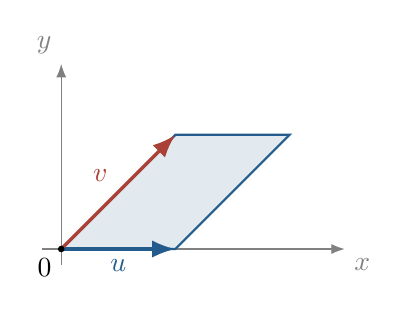
\begin{tikzpicture}[>=Latex,scale=1.0]
 \draw[->,gray] (-0.25,0) -- (3.6,0)
   node[below right] {\(x\)};
 \draw[->,gray] (0,-0.2) -- (0,2.35)
   node[above left] {\(y\)};
 \filldraw[fill=manifoldblue!13,draw=manifoldblue,thick]
   (0,0)--(1.45,0)--(2.9,1.45)--(1.45,1.45)--cycle;
 \draw[->,very thick,manifoldblue] (0,0)--(1.45,0)
   node[midway,below] {\(u\)};
 \draw[->,very thick,manifoldred] (0,0)--(1.45,1.45)
   node[midway,above left] {\(v\)};
 \fill (0,0) circle (1.2pt);
 \node[below left] at (0,0) {\(0\)};
\end{tikzpicture}
\caption{Równoległobok rozpięty przez
\(u=(1,0)^{\mathsf T}\) i \(v=(1,1)^{\mathsf T}\).
Macierz o tych kolumnach ma wyznacznik \(1\).
Rysunek ma charakter poglądowy.}
\label{fig:lin6-rownoleglobok}
\end{figure}

\section{Podsumowanie}
\label{sec:lin6-podsumowanie}

Wyznacznik jest jedyną znormalizowaną
funkcją wieloliniową i naprzemienną
wierszy macierzy kwadratowej.
Definicja przez permutacje działa
nad każdym ciałem, także w charakterystyce \(2\).
Operacje elementarne umożliwiają jego
obliczenie przez redukcję do macierzy
trójkątnej. Zachodzi
\(\det(AB)=\det A\det B\),
a macierz jest odwracalna dokładnie
wtedy, gdy jej wyznacznik jest niezerowy.
Rozwinięcie Laplace'a prowadzi do
macierzy dołączonej i wzoru na odwrotność,
natomiast wzory Cramera podają
współrzędne rozwiązania zgodnego układu
kwadratowego z odwracalną macierzą.
Wyznacznik endomorfizmu nie zależy
od wyboru jego uporządkowanej bazy.

\chapter{Przestrzeń dualna i odwzorowania dualne}
\label{ch:lin7-przestrzen-dualna}
\index{przestrzeń dualna@Przestrzeń dualna}
\index{funkcjonał liniowy@Funkcjonał liniowy}
\index{anihilator@Anihilator}
\index{odwzorowanie dualne@Odwzorowanie dualne}
\index{bidualność@Bidualność}

\noindent\textbf{Cel rozdziału.}
Do tej pory badaliśmy wektory i odwzorowania
liniowe pomiędzy przestrzeniami wektorowymi.
Teraz każdemu wektorowi przyporządkujemy
możliwość oceniania go przez funkcjonały
liniowe, a każdemu odwzorowaniu liniowemu
--- odpowiadające mu odwzorowanie dualne.
Uzasadnimy konstrukcję baz dualnych,
anihilatorów i naturalne zanurzenie przestrzeni
w jej przestrzeń bidualną. Na końcu pokażemy,
jak z tego punktu widzenia rozumieć
ślad endomorfizmu.

W całym rozdziale \(K\) jest dowolnym ciałem,
\(0_K\ne1_K\), a \(V,W,Z\) oznaczają przestrzenie
wektorowe nad \(K\). Nie zakładamy, że
charakterystyka \(K\) jest różna od \(2\).
Z wyjątkiem wyraźnie oznaczonych uwag
o wymiarze nieskończonym wszystkie twierdzenia
dotyczą przestrzeni skończenie wymiarowych;
dopuszczamy także wymiar \(0\).
W razie potrzeby zapis \(\operatorname{Hom}_K(V,W)\)
ma znaczenie ustalone w
Rozdziale~\ref{ch:lin3-odwzorowania-liniowe}.

\section{Funkcjonały liniowe i przestrzeń dualna}
\label{sec:lin7-funkcjonaly}

\begin{definicja}[Funkcjonał i przestrzeń dualna]
\label{def:lin7-dual}
\emph{Funkcjonałem liniowym} na \(V\)
nazywamy odwzorowanie liniowe
\(\varphi\colon V\to K\), gdzie \(K\)
traktujemy jako jednowymiarową
przestrzeń wektorową nad sobą.
\emph{Przestrzeń dualna} do \(V\) to
\[
 V^*:=\operatorname{Hom}_K(V,K).
\]
Dodawanie i mnożenie funkcjonałów
przez skalary określamy punktowo:
\((\varphi+\psi)(v)=\varphi(v)+\psi(v)\)
oraz \((a\varphi)(v)=a\varphi(v)\).
Parę \((\varphi,v)\in V^*\times V\)
łączymy zapisem
\(\langle\varphi,v\rangle:=\varphi(v)\).
\end{definicja}

\begin{stwierdzenie}[Liniowość ewaluacji]
\label{prop:lin7-ewaluacja}
Dla dowolnych \(\varphi,\psi\in V^*\),
\(v,w\in V\) i \(a,b\in K\) zachodzi
\[
 \begin{aligned}
 \langle a\varphi+b\psi,v\rangle
   &=a\langle\varphi,v\rangle
     +b\langle\psi,v\rangle,\\
 \langle\varphi,av+bw\rangle
   &=a\langle\varphi,v\rangle
     +b\langle\varphi,w\rangle.
 \end{aligned}
\]
Zatem ewaluacja jest funkcją
dwuliniową \(V^*\times V\to K\).
Jeżeli \(\dim V<\infty\) i \(v\ne0\),
to istnieje \(\varphi\in V^*\)
o \(\varphi(v)\ne0_K\).
\end{stwierdzenie}
\begin{proof}
Pierwsza równość wynika z punktowego
określenia działań w \(V^*\),
a druga z liniowości \(\varphi\).
Dla \(v\ne0\) jednoelementowy zbiór
\(\{v\}\) jest liniowo niezależny.
Uzupełnijmy go do bazy
\((v,v_2,\ldots,v_n)\) przestrzeni \(V\),
co jest możliwe na mocy
Twierdzenia~\ref{thm:lin-uzupelnianie-skonczone}.
Przyporządkowanie
\(v\mapsto1_K\), \(v_i\mapsto0_K\)
dla \(i\geq2\) przedłuża się
jednoznacznie do funkcjonału liniowego
na mocy
Twierdzenia~\ref{thm:lin3-przedluzenie-z-bazy}.
Dla niego \(\varphi(v)=1_K\ne0_K\).
\end{proof}

\begin{przyklad}[Funkcjonały współrzędnych]
\label{prz:lin7-wspolrzedne}
Niech \(V=K^3\). Wzory
\[
 \varphi(x,y,z)=2x-y+3z,\qquad
 \psi(x,y,z)=x+z
\]
określają funkcjonały liniowe.
Każdy funkcjonał
\(\lambda\colon K^3\to K\)
ma postać
\(\lambda(x,y,z)=ax+by+cz\)
dla dokładnie jednej trójki
\((a,b,c)\in K^3\), ponieważ
wartości na wektorach standardowych
wyznaczają go jednoznacznie.
Współczynniki \(2,-1,3\)
interpretujemy w dowolnym ciele \(K\);
w szczególności mogą się one
upraszczać w dodatniej charakterystyce.
\end{przyklad}

\begin{uwaga}[Algebraiczna przestrzeń dualna nie wymaga topologii]
\label{rem:lin7-dual-algebraiczny}
W definicji \(V^*\) nie występują
norma, iloczyn skalarny ani topologia.
Wszystkie funkcjonały są liniowe,
ale nie narzucamy na nie dodatkowego
warunku ciągłości. Jeśli w późniejszych
rozdziałach pojawi się norma, przestrzeń
ciągłych funkcjonałów liniowych będzie
wymagała osobnej definicji.
\end{uwaga}

\section{Bazy dualne i ich współrzędne}
\label{sec:lin7-baza-dualna}

\begin{definicja}[Baza dualna]
\label{def:lin7-baza-dualna}
Niech \(\dim V=n<\infty\) i
\(B=(v_1,\ldots,v_n)\) będzie
uporządkowaną bazą \(V\).
Dla każdego \(i\in\{1,\ldots,n\}\)
\emph{funkcjonałem dualnym}
do wektora \(v_i\) nazywamy
jedyny funkcjonał \(v^i\in V^*\)
spełniający
\[
 v^i(v_j)=\delta_{ij}
 \qquad (1\leq j\leq n).
\]
Układ \(B^*=(v^1,\ldots,v^n)\)
nazywamy \emph{bazą dualną} do \(B\).
W przypadku \(n=0\) obie bazy
są pustymi układami.
\end{definicja}

\begin{twierdzenie}[Istnienie i własność bazy dualnej]
\label{thm:lin7-baza-dualna}
Niech \(V\) będzie przestrzenią nad \(K\)
o wymiarze \(n<\infty\), a
\(B=(v_1,\ldots,v_n)\) jej bazą.
Wówczas funkcjonały
\(v^1,\ldots,v^n\) istnieją,
są jednoznaczne i tworzą bazę \(V^*\).
Dla każdych \(v\in V\) i
\(\varphi\in V^*\) zachodzą
tożsamości
\[
 v=\sum_{i=1}^{n}v^i(v)v_i,
 \qquad
 \varphi=\sum_{i=1}^{n}\varphi(v_i)v^i.
\]
W szczególności \(\dim V^*=\dim V=n\).
\end{twierdzenie}
\begin{proof}
Z
Twierdzenia~\ref{thm:lin3-przedluzenie-z-bazy}
wynika, że każde przyporządkowanie
skalarów wektorom bazy \(B\)
określa dokładnie jeden funkcjonał
liniowy. Dla każdego \(i\) wybierzmy
wartości \(\delta_{ij}\), co dowodzi
istnienia i jednoznaczności \(v^i\).

Niech \(v=\sum_j a_jv_j\).
Stosując \(v^i\), otrzymujemy
\(v^i(v)=\sum_j a_j\delta_{ij}=a_i\);
stąd pierwsza tożsamość.
Niech \(\varphi\in V^*\) i określmy
\(\psi=\sum_i\varphi(v_i)v^i\).
Dla każdego \(j\) mamy
\(\psi(v_j)=\sum_i\varphi(v_i)\delta_{ij}
=\varphi(v_j)\).
Dwa funkcjonały zgodne na bazie są
równe, więc \(\psi=\varphi\).
Oznacza to, że \(B^*\) rozpina \(V^*\).

Jeśli \(\sum_i a_iv^i=0\),
to po obliczeniu wartości w \(v_j\)
otrzymujemy \(a_j=0_K\) dla każdego
\(j\). Układ \(B^*\) jest więc
liniowo niezależny.
Dla \(n=0\) mamy \(V=\{0\}\);
jedyny funkcjonał z \(V\) do \(K\)
jest zerowy, a puste sumy
dają wymagane tożsamości.
\end{proof}

\begin{wniosek}[Współrzędne funkcjonału]
\label{cor:lin7-wspolrzedne-dualne}
Przy założeniach
Twierdzenia~\ref{thm:lin7-baza-dualna}
wektor kolumnowy współrzędnych
\(\varphi\in V^*\) w bazie dualnej
jest równy
\[
 [\varphi]_{B^*}
 =\bigl(\varphi(v_1),\ldots,\varphi(v_n)
   \bigr)^{\mathsf T}\in K^n.
\]
Jeżeli \([v]_B=(x_1,\ldots,x_n)^{\mathsf T}\),
to
\[
 \varphi(v)=[\varphi]_{B^*}^{\mathsf T}[v]_B
 =\sum_{i=1}^n \varphi(v_i)x_i.
\]
\end{wniosek}
\begin{proof}
Pierwsze twierdzenie daje rozwinięcie
\(\varphi=\sum_i\varphi(v_i)v^i\),
czyli wskazane współrzędne.
Ponieważ \(v=\sum_i x_iv_i\),
liniowość \(\varphi\) daje drugą równość.
Dla \(n=0\) suma jest pusta i wynosi
\(0_K\).
\end{proof}

\begin{przyklad}[Baza dualna w \(\mathbb R^2\)]
\label{prz:lin7-baza-dualna-r2}
Niech \(V=\mathbb R^2\) i
\(B=(v_1,v_2)\), gdzie
\(v_1=(1,1)^{\mathsf T}\) i
\(v_2=(1,-1)^{\mathsf T}\).
Dla \(x=(s,t)^{\mathsf T}\) rozwiązanie
\(x=av_1+bv_2\) daje
\(a=(s+t)/2\), \(b=(s-t)/2\).
Zatem
\[
 v^1(s,t)=\frac{s+t}{2},\qquad
 v^2(s,t)=\frac{s-t}{2}.
\]
Istotnie \(v^1(v_1)=v^2(v_2)=1\)
i \(v^1(v_2)=v^2(v_1)=0\).
Wzory wykorzystują dzielenie przez
\(2\), dlatego ten konkretny przykład
dotyczy \(\mathbb R\), a nie ciała
charakterystyki \(2\).
\end{przyklad}

\begin{twierdzenie}[Zmiana bazy dualnej]
\label{thm:lin7-zmiana-bazy-dualnej}
Niech \(V\) ma wymiar \(n<\infty\),
a \(B=(v_1,\ldots,v_n)\) i
\(C=(w_1,\ldots,w_n)\) będą bazami
uporządkowanymi. Niech \(P\in
\operatorname{Mat}_{n\times n}(K)\)
będzie macierzą przejścia określoną
równością
\[
 [v]_B=P[v]_C\qquad(v\in V).
\]
Wtedy dla każdego \(\varphi\in V^*\)
zachodzi
\[
 [\varphi]_{C^*}=P^{\mathsf T}
 [\varphi]_{B^*},
\]
a funkcjonały bazowe spełniają
\[
 w^j=\sum_{i=1}^n (P^{-1})_{ji}v^i,
 \qquad 1\leq j\leq n.
\]
\end{twierdzenie}
\begin{proof}
Kolumna \(j\) macierzy \(P\)
zawiera współrzędne \(w_j\) w bazie
\(B\), więc
\(w_j=\sum_i p_{ij}v_i\).
Dla każdego \(\varphi\in V^*\)
otrzymujemy
\(\varphi(w_j)=\sum_i p_{ij}\varphi(v_i)\).
Z
Wniosku~\ref{cor:lin7-wspolrzedne-dualne}
wynika, że jest to dokładnie
\(j\)-ta współrzędna wektora
\(P^{\mathsf T}[\varphi]_{B^*}\).
Dowodzi to pierwszego wzoru.

Macierz współrzędnych wartości
\((v^i(w_j))_{i,j}\) jest równa \(P\).
Pisząc \(w^j=\sum_i c_{ji}v^i\)
i podstawiając \(w_k\), otrzymujemy
warunek
\(\sum_i c_{ji}p_{ik}=\delta_{jk}\).
Zatem macierz \(C=(c_{ji})\)
spełnia \(CP=I_n\), czyli
\(C=P^{-1}\). Daje to drugi wzór.
Dla \(n=0\) macierz przejścia to
\(I_0\), a wszystkie równości są puste.
\end{proof}

\begin{uwaga}[Brak kanonicznej identyfikacji \(V\) i \(V^*\)]
\label{rem:lin7-niekanoniczna}
Równość wymiarów gwarantuje
istnienie izomorfizmu \(V\cong V^*\),
lecz powyższy wybór
\(v_i\mapsto v^i\) zależy od bazy.
Przy jej zmianie wektory
i funkcjonały mają odmienne reguły
przekształcania współrzędnych.
Nie należy więc utożsamiać
\(V\) z \(V^*\) bez dodatkowej struktury.
\end{uwaga}

\section{Anihilatory podprzestrzeni}
\label{sec:lin7-anihilatory}

\begin{definicja}[Anihilator]
\label{def:lin7-anihilator}
Niech \(U\) będzie podprzestrzenią
przestrzeni wektorowej \(V\).
Jej \emph{anihilatorem} nazywamy
\[
 U^\circ:=
 \{\varphi\in V^*:\ \varphi(u)=0_K
                 \text{ dla każdego }u\in U\}.
\]
Jest to podprzestrzeń \(V^*\).
Dla podprzestrzeni \(S\subset V^*\)
oznaczamy również przez
\[
 S_\circ:=
 \{v\in V:\ \varphi(v)=0_K
                   \text{ dla każdego }\varphi\in S\}
\]
jej anihilator w \(V\).
\end{definicja}

\begin{stwierdzenie}[Monotoniczność i przypadki skrajne]
\label{prop:lin7-anihilator-wlasnosci}
Niech \(V\) będzie skończenie wymiarowa,
a \(U_1,U_2\subset V\) podprzestrzeniami.
Wtedy
\[
 U_1\subset U_2
 \quad\Longrightarrow\quad
 U_2^\circ\subset U_1^\circ,
 \qquad
 \{0\}^\circ=V^*,\quad
 V^\circ=\{0\}.
\]
Dla dowolnych podprzestrzeni \(U_1,U_2\)
zachodzi ponadto
\[
 (U_1+U_2)^\circ=U_1^\circ\cap U_2^\circ.
\]
\end{stwierdzenie}
\begin{proof}
Funkcjonał zerujący się na większej
podprzestrzeni zeruje się na mniejszej,
co daje pierwszą inkluzję.
Każdy funkcjonał zeruje się w \(0\),
zaś funkcjonał zerujący się na całym
\(V\) jest funkcjonałem zerowym.
Wreszcie
\(\varphi(u_1+u_2)=0_K\)
dla wszystkich \(u_1\in U_1\),
\(u_2\in U_2\) wtedy i tylko wtedy,
gdy \(\varphi\) zeruje się na obu
podprzestrzeniach: dla implikacji
w prawo podstawiamy kolejno
\(u_2=0\) i \(u_1=0\);
dla implikacji odwrotnej korzystamy
z liniowości \(\varphi\).
\end{proof}

\begin{twierdzenie}[Wymiar anihilatora]
\label{thm:lin7-wymiar-anihilatora}
Niech \(V\) ma wymiar \(n<\infty\),
a \(U\subset V\) będzie
podprzestrzenią o wymiarze \(r\).
Wtedy
\[
 \dim U^\circ=n-r.
\]
Co więcej, jeśli
\(B=(u_1,\ldots,u_r,v_{r+1},\ldots,v_n)\)
jest bazą \(V\), w której pierwsze
\(r\) wektorów tworzy bazę \(U\),
to
\[
 U^\circ=
 \operatorname{span}\{v^{r+1},\ldots,v^n\},
\]
gdzie \(v^{r+1},\ldots,v^n\)
są odpowiednimi elementami
bazy dualnej \(B^*\).
\end{twierdzenie}
\begin{proof}
Dzięki twierdzeniu o uzupełnianiu
bazy możemy wybrać bazę \(B\)
o wskazanej postaci. Każdy funkcjonał
\(\varphi\in V^*\) zapisujemy
jednoznacznie jako
\[
 \varphi=\sum_{i=1}^{r}
          \varphi(u_i)u^i
        +\sum_{i=r+1}^{n}
          \varphi(v_i)v^i.
\]
Funkcjonał zeruje się na \(U\)
wtedy i tylko wtedy, gdy
\(\varphi(u_i)=0_K\) dla wszystkich
\(1\leq i\leq r\), ponieważ wektory
\(u_1,\ldots,u_r\) rozpinają \(U\).
Zatem pozostaje druga suma.
Odpowiednie funkcjonały tworzą
liniowo niezależną rodzinę
długości \(n-r\) i generują
\(U^\circ\). To daje obie tezy.
Obejmuje to \(U=\{0\}\),
\(U=V\), a także \(n=0\).
\end{proof}

\begin{wniosek}[Anihilator anihilatora]
\label{cor:lin7-podwojny-anihilator}
Jeżeli \(V\) ma skończony wymiar,
a \(U\subset V\) i \(S\subset V^*\)
są podprzestrzeniami, to
\[
 (U^\circ)_\circ=U,\qquad
 (S_\circ)^\circ=S.
\]
\end{wniosek}
\begin{proof}
Przyjmijmy bazę \(B\) jak
w Twierdzeniu~\ref{thm:lin7-wymiar-anihilatora}.
Wtedy \(U^\circ\) jest rozpięty
przez \(v^{r+1},\ldots,v^n\).
Wektor \(x=\sum_{i=1}^n x_iv_i\)
należy do \((U^\circ)_\circ\)
wtedy i tylko wtedy, gdy
\(x_{r+1}=\cdots=x_n=0_K\).
Oznacza to dokładnie, że \(x\in U\).

Dla drugiej równości wybierzmy bazę
\((\varphi_1,\ldots,\varphi_s)\)
przestrzeni \(S\), gdzie \(s=\dim S\).
Określmy odwzorowanie liniowe
\[
 L\colon V\to K^s,\qquad
 L(v)=(\varphi_1(v),\ldots,\varphi_s(v)).
\]
Jest ono surjektywne. Istotnie,
gdyby \(\operatorname{im}L\ne K^s\),
istniałby niezerowy funkcjonał
\(\eta\in(K^s)^*\) zerujący się
na \(\operatorname{im}L\):
wybieramy bazę obrazu, uzupełniamy
ją do bazy \(K^s\) i nadajemy
wartość \(1_K\) jednemu z
uzupełniających wektorów,
a pozostałym wartość \(0_K\).
W bazie standardowej funkcjonał
\(\eta\) ma pewne współczynniki
\(a_1,\ldots,a_s\), nie wszystkie zerowe.
Jednak \(\eta\circ L=0\)
oznaczałoby
\(\sum_{i=1}^s a_i\varphi_i=0\),
wbrew niezależności liniowej bazy \(S\).
Zatem \(\operatorname{rk}L=s\).

Z definicji \(\ker L=S_\circ\).
Twierdzenie o wymiarze jądra
i obrazu daje
\(\dim S_\circ=n-s\), a
Twierdzenie~\ref{thm:lin7-wymiar-anihilatora}
zapewnia
\(\dim(S_\circ)^\circ=s\).
Każdy funkcjonał z \(S\) zeruje się
na \(S_\circ\), czyli
\(S\subset(S_\circ)^\circ\).
Inkluzja między podprzestrzeniami
tego samego wymiaru jest równością.
W przypadku \(s=0\) odwzorowanie
\(L\colon V\to K^0\) jest surjektywne
i ten sam argument daje wynik.
\end{proof}

\begin{przyklad}[Anihilator płaszczyzny]
\label{prz:lin7-anihilator-r3}
Niech \(V=\mathbb R^3\), a
\[
 U=\{(x,y,z)\in\mathbb R^3:
                 x+2y-z=0\}.
\]
Przestrzeń \(U\) ma wymiar \(2\).
Funkcjonał \(\ell(x,y,z)=x+2y-z\)
zeruje się na \(U\), więc
\(\ell\in U^\circ\).
Ponieważ \(\ell\ne0\), a
\(\dim U^\circ=3-2=1\),
otrzymujemy
\(U^\circ=\operatorname{span}\{\ell\}\).
Przykład pokazuje, że jedno równanie
liniowe opisujące podprzestrzeń
jest w istocie elementem przestrzeni dualnej.
\end{przyklad}

\begin{twierdzenie}[Anihilator przecięcia]
\label{thm:lin7-anihilator-przeciecia}
Jeśli \(V\) ma skończony wymiar
i \(U_1,U_2\subset V\) są
podprzestrzeniami, to
\[
 (U_1\cap U_2)^\circ
 =U_1^\circ+U_2^\circ.
\]
\end{twierdzenie}
\begin{proof}
Jeśli
\(\varphi=\varphi_1+\varphi_2\),
gdzie \(\varphi_i\in U_i^\circ\),
to \(\varphi\) zeruje się na
\(U_1\cap U_2\), więc
\(U_1^\circ+U_2^\circ
 \subset (U_1\cap U_2)^\circ\).
Dla równości wymiarów
korzystamy z
Twierdzenia~\ref{thm:lin2-wzor-wymiarowy},
z równości
\((U_1+U_2)^\circ
=U_1^\circ\cap U_2^\circ\)
i ze wzoru na wymiar anihilatora.
Mamy
\[
\begin{aligned}
 \dim(U_1^\circ+U_2^\circ)
 &= (n-\dim U_1)+(n-\dim U_2)\\
 &\quad -(n-\dim(U_1+U_2))\\
 &=n-\dim(U_1\cap U_2)\\
 &=\dim(U_1\cap U_2)^\circ.
\end{aligned}
\]
Inkluzja podprzestrzeni o tych
samych skończonych wymiarach
jest równością.
\end{proof}

\section{Przestrzeń dualna do ilorazu i rozszerzanie funkcjonałów}
\label{sec:lin7-dual-ilorazu}

\begin{twierdzenie}[Rozszerzenie funkcjonału z podprzestrzeni]
\label{thm:lin7-rozszerzanie}
Niech \(V\) ma skończony wymiar,
\(U\subset V\) będzie podprzestrzenią,
a \(\lambda\in U^*\).
Wówczas istnieje
\(\widetilde\lambda\in V^*\)
spełniający
\(\widetilde\lambda(u)=\lambda(u)\)
dla każdego \(u\in U\).
Nie twierdzimy, że to rozszerzenie
jest jednoznaczne.
\end{twierdzenie}
\begin{proof}
Wybierzmy bazę
\((u_1,\ldots,u_r)\) przestrzeni \(U\).
Uzupełnijmy ją do bazy \(V\)
o pozostałych wektorach
\(v_{r+1},\ldots,v_n\).
Wartości \(\lambda(u_i)\)
dla \(1\leq i\leq r\)
zachowujemy, a na wektorach
\(v_{r+1},\ldots,v_n\)
ustalamy wartości \(0_K\).
Twierdzenie o odwzorowaniu zadanym
na bazie daje jednoznaczny funkcjonał
na \(V\) o tych wartościach.
Jego ograniczenie do \(U\)
jest równe \(\lambda\),
gdyż oba funkcjonały są liniowe
i zgodne na bazie \(U\).
Dla \(U=\{0\}\) jedyny funkcjonał
na \(U\) jest zerowy i wystarcza
wybrać \(\widetilde\lambda=0\).
\end{proof}

\begin{twierdzenie}[Przestrzeń dualna do ilorazu]
\label{thm:lin7-dual-ilorazu}
Niech \(V\) będzie skończenie wymiarowa,
\(U\subset V\) podprzestrzenią,
a \(q\colon V\to V/U\),
\(q(v)=v+U\), odwzorowaniem ilorazowym.
Odwzorowanie
\[
 q^*\colon (V/U)^*\longrightarrow V^*,
 \qquad q^*(\psi)=\psi\circ q,
\]
jest liniowe i różnowartościowe,
a jego obrazem jest dokładnie
\(U^\circ\).
W konsekwencji
\[
 (V/U)^*\cong U^\circ.
\]
\end{twierdzenie}
\begin{proof}
Złożenie dwóch odwzorowań liniowych
jest liniowe, więc \(q^*\)
jest dobrze określone.
Jego liniowość wynika
z punktowych działań na funkcjonałach.
Jeśli \(\psi\circ q=0\),
to z surjektywności \(q\)
wynika \(\psi=0\), więc \(q^*\)
jest różnowartościowe.
Jeśli \(\psi\in(V/U)^*\),
to dla \(u\in U\) mamy \(q(u)=0\)
oraz \((\psi\circ q)(u)=0_K\).
Stąd \(\operatorname{im}q^*\subset U^\circ\).

Odwrotnie, jeśli
\(\varphi\in U^\circ\),
to wzór
\(\psi(v+U):=\varphi(v)\)
jest dobrze określony:
gdy \(v+U=w+U\), wówczas
\(v-w\in U\), a więc
\(\varphi(v-w)=0_K\).
Wzór określa funkcjonał liniowy
na \(V/U\), dla którego
\(\psi\circ q=\varphi\).
Zatem \(\operatorname{im}q^*=U^\circ\).
\end{proof}

\begin{wniosek}[Przestrzeń dualna do sumy prostej]
\label{cor:lin7-dual-sumy-prostej}
Niech \(V=U_1\oplus U_2\)
będzie wewnętrzną sumą prostą
skończenie wymiarowych podprzestrzeni.
Wtedy odwzorowanie
\[
 V^*\longrightarrow U_1^*\oplus U_2^*,
 \qquad
 \varphi\longmapsto
   (\varphi|_{U_1},\varphi|_{U_2})
\]
jest izomorfizmem przestrzeni
wektorowych nad \(K\).
\end{wniosek}
\begin{proof}
Odwzorowanie jest liniowe.
Jeśli oba ograniczenia funkcjonału
są zerowe, to dla dowolnego
\(v=u_1+u_2\) mamy
\(\varphi(v)=0_K+0_K=0_K\);
odwzorowanie jest więc iniektywne.
Dla dowolnych
\(\lambda_i\in U_i^*\)
wzór
\(\varphi(u_1+u_2)=
\lambda_1(u_1)+\lambda_2(u_2)\)
jest dobrze określony, ponieważ
rozkład w sumie prostej jest
jednoznaczny. Jest liniowy i
ma wymagane ograniczenia, zatem
odwzorowanie jest surjektywne.
\end{proof}

\section{Odwzorowanie dualne i macierz transponowana}
\label{sec:lin7-odwzorowanie-dualne}

\begin{definicja}[Odwzorowanie dualne]
\label{def:lin7-odwzorowanie-dualne}
Dla dowolnego odwzorowania liniowego
\(T\colon V\to W\)
\emph{odwzorowaniem dualnym} do \(T\)
nazywamy
\[
 T^*\colon W^*\to V^*,
 \qquad
 (T^*\psi)(v):=\psi(Tv),
 \qquad \psi\in W^*,\ v\in V.
\]
A więc \(T^*(\psi)=\psi\circ T\).
Kierunek działania jest przeciwny
do kierunku \(T\).
\end{definicja}

\begin{twierdzenie}[Liniowość i odwracanie składania]
\label{thm:lin7-funktorialnosc}
Niech \(T\colon V\to W\)
i \(S\colon W\to Z\) będą
odwzorowaniami liniowymi.
Wówczas \(T^*\colon W^*\to V^*\)
jest liniowe oraz
\[
 (S\circ T)^*=T^*\circ S^*,
 \qquad
 (\operatorname{id}_V)^*
 =\operatorname{id}_{V^*}.
\]
Jeżeli \(T\) jest izomorfizmem,
to \(T^*\) jest izomorfizmem oraz
\[
 (T^*)^{-1}=(T^{-1})^*.
\]
\end{twierdzenie}
\begin{proof}
Dla \(\psi_1,\psi_2\in W^*\),
\(a,b\in K\) i \(v\in V\) mamy
\[
 \bigl(T^*(a\psi_1+b\psi_2)\bigr)(v)
 =(a\psi_1+b\psi_2)(Tv)
 =a(T^*\psi_1)(v)+b(T^*\psi_2)(v).
\]
Ponieważ funkcjonały o identycznych
wartościach na wszystkich wektorach
są równe, dowodzi to liniowości \(T^*\).

Dla \(\eta\in Z^*\) i \(v\in V\)
obliczamy
\[
 \bigl((S\circ T)^*\eta\bigr)(v)
 =\eta(S(Tv))
 =\bigl(T^*(S^*\eta)\bigr)(v),
\]
co daje równość złożeń.
Wzór dla identyczności wynika
bezpośrednio z definicji.

Jeśli \(T^{-1}\) istnieje,
to odwracanie składania daje
\[
 T^*\circ(T^{-1})^*
 =(T^{-1}\circ T)^*
 =\operatorname{id}_{V^*}
\]
oraz
\((T^{-1})^*\circ T^*
 =\operatorname{id}_{W^*}\).
Zatem \((T^{-1})^*\)
jest dwustronną odwrotnością \(T^*\).
\end{proof}

\begin{twierdzenie}[Macierz odwzorowania dualnego]
\label{thm:lin7-macierz-dualnego}
Niech \(\dim V=n<\infty\) i
\(\dim W=m<\infty\).
Wybierzmy uporządkowane bazy
\(B=(v_1,\ldots,v_n)\) w \(V\)
oraz \(C=(w_1,\ldots,w_m)\) w \(W\).
Jeżeli \(A=(a_{ij})\in
\operatorname{Mat}_{m\times n}(K)\)
jest macierzą odwzorowania liniowego
\(T\colon V\to W\) w bazach \(B,C\),
to macierz odwzorowania
\(T^*\colon W^*\to V^*\)
w bazach dualnych \(C^*,B^*\)
jest równa \(A^{\mathsf T}\).
W szczególności
\[
 [T^*\psi]_{B^*}
  =A^{\mathsf T}[\psi]_{C^*}
 \qquad(\psi\in W^*).
\]
\end{twierdzenie}
\begin{proof}
Z definicji macierzy odwzorowania
\(Tv_j=\sum_{i=1}^m a_{ij}w_i\).
Dla funkcjonału \(w^i\)
z bazy dualnej \(C^*\)
i \(v_j\in B\) mamy
\[
 (T^*w^i)(v_j)
 =w^i(Tv_j)
 =w^i\Bigl(\sum_{k=1}^m a_{kj}w_k\Bigr)
 =a_{ij}.
\]
Zatem \(j\)-ta współrzędna
funkcjonału \(T^*w^i\)
w bazie \(B^*\) jest równa \(a_{ij}\).
Jest to element w wierszu \(j\)
i kolumnie \(i\) macierzy \(T^*\),
czyli element \((A^{\mathsf T})_{ji}\).
Gdy \(n=0\) lub \(m=0\),
obliczenie dotyczy pustych rodzin
i nadal daje właściwą macierz
rozmiaru \(n\times m\).
\end{proof}

\begin{figure}[!htbp]
\centering
\begin{tikzpicture}[>=Latex,node distance=33mm and 37mm]
 \node (wstar) {\(W^*\)};
 \node[right=of wstar] (vstar) {\(V^*\)};
 \node[below=of wstar] (km) {\(K^m\)};
 \node[right=of km] (kn) {\(K^n\)};
 \draw[->] (wstar)--node[above]{\(T^*\)}(vstar);
 \draw[->] (wstar)--node[left]{\([\cdot]_{C^*}\)}(km);
 \draw[->] (vstar)--node[right]{\([\cdot]_{B^*}\)}(kn);
 \draw[->] (km)--node[below]{\(A^{\mathsf T}\)}(kn);
\end{tikzpicture}
\caption{Odwzorowanie dualne zmienia kierunek
względem \(T\colon V\to W\).
W bazach dualnych jego macierzą jest
transpozycja macierzy \(T\).}
\label{fig:lin7-dualne-diagram}
\end{figure}

\begin{przyklad}[Działanie odwzorowania dualnego]
\label{prz:lin7-transpozycja}
Niech \(V=\mathbb R^2\), \(W=\mathbb R^3\)
i niech w bazach standardowych
odwzorowanie \(T\) ma macierz
\[
 A=\begin{pmatrix}
 1&2\\
 -1&0\\
 3&1
 \end{pmatrix}.
\]
Dla \(\psi(x,y,z)=2x-y+z\)
kolumna współrzędnych \(\psi\)
w bazie dualnej wynosi
\((2,-1,1)^{\mathsf T}\).
Zatem
\[
 [T^*\psi]_{B^*}
 =\begin{pmatrix}1&-1&3\\2&0&1\end{pmatrix}
  \begin{pmatrix}2\\-1\\1\end{pmatrix}
 =\begin{pmatrix}6\\5\end{pmatrix}.
\]
Bez użycia macierzy:
\(T(s,t)=(s+2t,-s,3s+t)\),
więc
\(\psi(T(s,t))=2(s+2t)+s+(3s+t)=6s+5t\).
Obie metody dają ten sam funkcjonał.
\end{przyklad}

\section{Jądro, obraz i rząd odwzorowania dualnego}
\label{sec:lin7-dual-rzad}

\begin{twierdzenie}[Jądro i obraz odwzorowania dualnego]
\label{thm:lin7-jadro-obraz-dualnego}
Niech \(V,W\) będą
skończenie wymiarowymi przestrzeniami
nad \(K\), a \(T\colon V\to W\)
odwzorowaniem liniowym. Wtedy
\[
 \ker T^*=(\operatorname{im}T)^\circ
 \quad\text{(podprzestrzeń \(W^*\))},
 \qquad
 \operatorname{im}T^*=(\ker T)^\circ
 \quad\text{(podprzestrzeń \(V^*\))}.
\]
W szczególności
\[
 \operatorname{rk}T^*=\operatorname{rk}T.
\]
\end{twierdzenie}
\begin{proof}
Dla \(\psi\in W^*\) warunek
\(\psi\in\ker T^*\)
jest równoważny
\((T^*\psi)(v)=\psi(Tv)=0_K\)
dla każdego \(v\in V\).
Oznacza to dokładnie
\(\psi|_{\operatorname{im}T}=0\),
czyli pierwszą równość.

Jeśli \(\psi\in W^*\) i \(v\in\ker T\),
to \((T^*\psi)(v)=\psi(0)=0_K\).
Daje to inkluzję
\(\operatorname{im}T^*
 \subset(\ker T)^\circ\).

Dla drugiej inkluzji niech
\(\varphi\in(\ker T)^\circ\).
Na \(\operatorname{im}T\subset W\)
określmy funkcjonał
\(\lambda(Tv)=\varphi(v)\).
Jeżeli \(Tv=Tw\), to \(v-w\in\ker T\),
a więc \(\varphi(v-w)=0_K\);
wzór jest zatem dobrze określony.
Jest liniowy, ponieważ
\(\lambda(T(av+bw))
=\varphi(av+bw)
=a\varphi(v)+b\varphi(w)\).
Na mocy
Twierdzenia~\ref{thm:lin7-rozszerzanie}
istnieje funkcjonał \(\psi\in W^*\)
rozszerzający \(\lambda\).
Dla każdego \(v\in V\) otrzymujemy
\((T^*\psi)(v)=\psi(Tv)=\varphi(v)\),
zatem \(\varphi=T^*\psi\).
Wykazaliśmy równość obrazów.

Z twierdzenia o wymiarze jądra
i obrazu oraz wzoru na wymiar
anihilatora wynika
\[
 \begin{aligned}
 \operatorname{rk}T^*
 &=\dim(\ker T)^\circ\\
 &=\dim V-\dim\ker T\\
 &=\operatorname{rk}T.
 \end{aligned}
\]
Rachunek obejmuje również
przypadki \(V=\{0\}\) i \(W=\{0\}\).
\end{proof}

\begin{wniosek}[Rząd macierzy i jej transpozycji]
\label{cor:lin7-rzad-transpozycji}
Dla dowolnych \(m,n\in\mathbb N_0\)
i macierzy \(A\in
\operatorname{Mat}_{m\times n}(K)\)
zachodzi
\[
 \operatorname{rk}A^{\mathsf T}
 =\operatorname{rk}A.
\]
Jest to równość rzędów kolumnowych,
uzyskana bez używania iloczynu
skalarnego na \(K^m\) lub \(K^n\).
\end{wniosek}
\begin{proof}
Niech \(T\colon K^n\to K^m\)
będzie odwzorowaniem \(T(x)=Ax\).
Jego odwzorowanie dualne ma
w bazach dualnych macierz
\(A^{\mathsf T}\) na mocy
Twierdzenia~\ref{thm:lin7-macierz-dualnego}.
Wynik wynika z
Twierdzenia~\ref{thm:lin7-jadro-obraz-dualnego}.
\end{proof}

\begin{wniosek}[Wzajemność iniektywności i surjektywności]
\label{cor:lin7-injekcja-surjekcja}
Niech \(V,W\) będą skończenie
wymiarowymi przestrzeniami,
a \(T\colon V\to W\) liniowym
odwzorowaniem. Wtedy
\[
 \begin{aligned}
 T\text{ jest surjektywne}
 &\quad\Longleftrightarrow\quad
 T^*\text{ jest iniektywne},\\
 T\text{ jest iniektywne}
 &\quad\Longleftrightarrow\quad
 T^*\text{ jest surjektywne}.
 \end{aligned}
\]
\end{wniosek}
\begin{proof}
Pierwszą równoważność otrzymujemy,
obliczając
\(\ker T^*=(\operatorname{im}T)^\circ\).
Anihilator podprzestrzeni
\(M\subset W\) jest zerowy dokładnie
wtedy, gdy \(M=W\), ponieważ
\(\dim M^\circ=\dim W-\dim M\).
Zatem \(\ker T^*=\{0\}\)
dokładnie wtedy, gdy
\(\operatorname{im}T=W\).

Drugą równoważność otrzymujemy z
\(\operatorname{im}T^*=(\ker T)^\circ\).
Anihilator \(\ker T\) jest całym \(V^*\)
wtedy i tylko wtedy, gdy \(\ker T=\{0\}\),
co można sprawdzić porównując wymiary.
\end{proof}

\section{Przestrzeń bidualna}
\label{sec:lin7-bidualnosc}

\begin{definicja}[Przestrzeń bidualna i odwzorowanie kanoniczne]
\label{def:lin7-bidual}
Przestrzenią \emph{bidualną} do \(V\)
nazywamy \(V^{**}:=(V^*)^*\).
Każdemu \(v\in V\) odpowiada
funkcjonał \(J_V(v)\in V^{**}\)
zdefiniowany przez
\[
 J_V(v)(\varphi):=\varphi(v)
 \qquad(\varphi\in V^*).
\]
Otrzymujemy odwzorowanie
\(J_V\colon V\to V^{**}\)
nazywane \emph{odwzorowaniem
kanonicznym do przestrzeni bidualnej}.
\end{definicja}

\begin{twierdzenie}[Bidualność w wymiarze skończonym]
\label{thm:lin7-bidualnosc}
Niech \(V\) będzie skończenie wymiarowa.
Wtedy \(J_V\colon V\to V^{**}\)
jest kanonicznym izomorfizmem
przestrzeni wektorowych.
Jeżeli \(B=(v_1,\ldots,v_n)\)
jest uporządkowaną bazą \(V\),
to \((J_V(v_1),\ldots,J_V(v_n))\)
jest bazą dualną do \(B^*\)
w przestrzeni \(V^{**}\).
\end{twierdzenie}
\begin{proof}
Dla każdego \(v\in V\)
funkcja \(\varphi\mapsto\varphi(v)\)
jest liniowa z \(V^*\) do \(K\),
zatem \(J_V(v)\in V^{**}\).
Dla \(a,b\in K\), \(v,w\in V\)
i dowolnego \(\varphi\in V^*\)
mamy
\[
 J_V(av+bw)(\varphi)
 =\varphi(av+bw)
 =aJ_V(v)(\varphi)
  +bJ_V(w)(\varphi).
\]
Stąd \(J_V\) jest liniowe.

Jeśli \(J_V(v)=0\), to
\(\varphi(v)=0_K\) dla każdego
\(\varphi\in V^*\).
Ze
Stwierdzenia~\ref{prop:lin7-ewaluacja}
wynika \(v=0\), więc \(J_V\)
jest iniektywne.
Z Twierdzenia~\ref{thm:lin7-baza-dualna}
otrzymujemy
\(\dim V^{**}=\dim V^*=\dim V\).
Liniowe odwzorowanie iniektywne
między skończenie wymiarowymi
przestrzeniami równego wymiaru
jest surjektywne, a więc \(J_V\)
jest izomorfizmem.

Ponadto
\(J_V(v_i)(v^j)=v^j(v_i)=\delta_{ij}\),
czyli obrazy wektorów bazy \(B\)
są elementami bazy dualnej
do \(B^*\). Dotyczy to także
przypadku \(n=0\).
\end{proof}

\begin{twierdzenie}[Naturalność identyfikacji z bidualem]
\label{thm:lin7-naturalnosc-bidualu}
Niech \(V,W\) będą skończenie
wymiarowymi przestrzeniami
i \(T\colon V\to W\) odwzorowaniem
liniowym. Wtedy
\[
 T^{**}\circ J_V=J_W\circ T,
\]
gdzie \(T^{**}:=(T^*)^*
\colon V^{**}\to W^{**}\).
W szczególności utożsamienie
\(V\cong V^{**}\) nie zależy
od wyboru bazy.
\end{twierdzenie}
\begin{proof}
Niech \(v\in V\) i \(\psi\in W^*\).
Z definicji odwzorowań dualnych
otrzymujemy
\[
 \begin{aligned}
 (T^{**}(J_Vv))(\psi)
 &=J_Vv(T^*\psi)\\
 &=(T^*\psi)(v)
 =\psi(Tv)
 =J_W(Tv)(\psi).
 \end{aligned}
\]
Oba elementy \(W^{**}\) mają
te same wartości na każdym
\(\psi\in W^*\), więc są równe.
Formuła definiująca \(J_V\)
nie wykorzystuje bazy;
ostatni wniosek jest więc
własnością samej konstrukcji.
\end{proof}

\begin{uwaga}[Wymiar nieskończony]
\label{rem:lin7-nieskonczony-bidual}
Dla dowolnej przestrzeni wektorowej
odwzorowanie \(J_V\) ma sens i jest
liniowe. Przy istnieniu baz Hamela
pozostaje iniektywne: niezerowy wektor
można włączyć do bazy i przypisać mu
wartość \(1_K\) funkcjonału liniowego.
W przestrzeniach nieskończenie
wymiarowych \(J_V\) nie musi być
surjektywne. Dlatego twierdzenie
o izomorfizmie sformułowaliśmy
wyłącznie w wymiarze skończonym.
\end{uwaga}

\section{Ślad endomorfizmu}
\label{sec:lin7-slad}

\begin{definicja}[Ślad macierzy]
\label{def:lin7-slad}
Niech \(n\in\mathbb N_0\) i
\(A=(a_{ij})\in\operatorname{Mat}_{n\times n}(K)\).
\emph{Śladem} \(A\) nazywamy
\[
 \operatorname{tr}A:=\sum_{i=1}^n a_{ii}.
\]
Dla \(n=0\) jest to pusta suma,
czyli \(\operatorname{tr}I_0=0_K\).
\end{definicja}

\begin{twierdzenie}[Liniowość i cykliczność śladu]
\label{thm:lin7-slad}
Niech \(n\in\mathbb N_0\).
Dla dowolnych macierzy
\(A,B\in\operatorname{Mat}_{n\times n}(K)\)
i \(a,b\in K\) mamy
\[
 \operatorname{tr}(aA+bB)
 =a\operatorname{tr}A+b\operatorname{tr}B,
 \qquad
 \operatorname{tr}(AB)
 =\operatorname{tr}(BA).
\]
Jeśli \(P\in\operatorname{Mat}_{n\times n}(K)\)
jest odwracalna, to
\[
 \operatorname{tr}(P^{-1}AP)
 =\operatorname{tr}A.
\]
Dlatego dla dowolnego endomorfizmu
\(T\colon V\to V\) skończenie
wymiarowej przestrzeni \(V\)
można poprawnie zdefiniować
\(\operatorname{tr}T\)
jako ślad macierzy \(T\)
w dowolnej uporządkowanej bazie.
\end{twierdzenie}
\begin{proof}
Liniowość wynika wprost ze wzoru
na ślad i punktowych działań
na macierzach. Dla cykliczności
rozpisujemy wyrazy diagonalne:
\[
 \begin{aligned}
 \operatorname{tr}(AB)
 &=\sum_{i=1}^n\sum_{j=1}^n a_{ij}b_{ji}\\
 &=\sum_{j=1}^n\sum_{i=1}^n b_{ji}a_{ij}
 =\operatorname{tr}(BA).
 \end{aligned}
\]
W drugim przejściu użyliśmy
przemienności mnożenia w ciele \(K\)
oraz możliwości zmiany kolejności
skończonych sum.

Dla odwracalnej macierzy \(P\)
cykliczność zastosowana do
\(P^{-1}A\) i \(P\) daje
\[
 \operatorname{tr}(P^{-1}AP)
 =\operatorname{tr}(PP^{-1}A)
 =\operatorname{tr}A.
\]
Macierze jednego endomorfizmu
w różnych bazach są podobne
na mocy
Wniosku~\ref{cor:lin4-podobienstwo},
więc ich ślady są jednakowe.
W wymiarze \(0\) wszystkie sumy
w dowodzie są puste; w szczególności
ślad jest równy \(0_K\).
\end{proof}

\begin{stwierdzenie}[Ślad odwzorowania rzędu co najwyżej jeden]
\label{prop:lin7-slad-rank-jeden}
Niech \(V\) będzie skończenie wymiarowa,
\(v\in V\) oraz \(\varphi\in V^*\).
Zdefiniujmy endomorfizm
\(R_{v,\varphi}\colon V\to V\) wzorem
\[
 R_{v,\varphi}(x):=\varphi(x)v.
\]
Wtedy \(\operatorname{rk}R_{v,\varphi}\leq1\)
i
\[
 \operatorname{tr}R_{v,\varphi}=\varphi(v).
\]
\end{stwierdzenie}
\begin{proof}
Obraz \(R_{v,\varphi}\)
zawiera się w \(\operatorname{span}\{v\}\),
więc jego wymiar jest co najwyżej \(1\).
Niech \(B=(v_1,\ldots,v_n)\)
będzie dowolną uporządkowaną bazą,
a \([v]_B=(c_1,\ldots,c_n)^{\mathsf T}\).
Ponieważ
\(R_{v,\varphi}(v_j)=\varphi(v_j)v\),
element \((i,j)\) macierzy
tego endomorfizmu jest równy
\(c_i\varphi(v_j)\).
Zatem jej ślad wynosi
\[
 \sum_{i=1}^n c_i\varphi(v_i)
 =\varphi\left(\sum_{i=1}^n c_iv_i\right)
 =\varphi(v).
\]
Dla \(V=\{0\}\) mamy \(v=0\),
funkcjonał zerowy i ślad \(0_K\),
więc wzór nadal zachodzi.
\end{proof}

\begin{przyklad}[Ślad a wyznacznik]
\label{prz:lin7-slad-wyznacznik}
Dla \(A=\begin{pmatrix}1&2\\0&3\end{pmatrix}\)
nad \(\mathbb R\) mamy
\(\operatorname{tr}A=1+3=4\),
a \(\det A=1\cdot3=3\).
Są to różne niezmienniki
podobieństwa. Dla
\(B=\begin{pmatrix}3&0\\0&1\end{pmatrix}\)
otrzymujemy ten sam ślad i
ten sam wyznacznik, lecz sama zgodność
tych dwóch liczb nie dowodzi podobieństwa
dowolnych macierzy.
\end{przyklad}

\section{Podsumowanie}
\label{sec:lin7-podsumowanie}

Przestrzeń dualna \(V^*\)
składa się ze wszystkich funkcjonałów
liniowych na \(V\). W wymiarze
skończonym każdej bazie \(V\)
odpowiada baza dualna, a współrzędne
funkcjonału są jego wartościami
na wektorach wyjściowej bazy.
Anihilator \(U^\circ\)
zawiera dokładnie funkcjonały
zerujące się na \(U\), przy czym
\(\dim U^\circ=\dim V-\dim U\).
Odwzorowaniu liniowemu \(T\colon V\to W\)
odpowiada odwzorowanie dualne
\(T^*\colon W^*\to V^*\)
o macierzy transponowanej.
Kanoniczny izomorfizm
\(V\to V^{**}\) istnieje
w wymiarze skończonym bez wyboru bazy;
nie należy go mylić z zależnym
od bazy izomorfizmem \(V\cong V^*\).
Ślad endomorfizmu, podobnie jak
wyznacznik, jest niezmiennikiem
zmiany bazy, lecz opisuje inną
własność odwzorowania.

\chapter{Odwzorowania wieloliniowe}
\label{ch:lin8-wieloliniowe}
\index{odwzorowanie wieloliniowe@Odwzorowanie wieloliniowe}
\index{forma wieloliniowa@Forma wieloliniowa}
\index{forma symetryczna@Forma symetryczna}
\index{forma naprzemienna@Forma naprzemienna}

\noindent\textbf{Cel rozdziału.}
Odwzorowania liniowe zachowują kombinacje liniowe
jednego argumentu. W wielu konstrukcjach potrzebujemy
funkcji zależnych od kilku wektorów, liniowych
w każdym z nich oddzielnie. Takie odwzorowania
opisują formy dwuliniowe, wyznaczniki i formy
o wyższej liczbie argumentów.
Wyprowadzimy ich wzory współrzędnych oraz zbadamy
symetrię, naprzemienność i związane z nimi
przestrzenie liniowe. Nie będziemy jeszcze
zakładać istnienia iloczynów tensorowych;
ich konstrukcja jest tematem Rozdziału~\ref{ch:lin10-iloczyny-tensorowe}.

W całym rozdziale \(K\) jest ciałem,
\(0_K\ne1_K\). Wszystkie przestrzenie
wektorowe występujące w twierdzeniach
o wymiarze są skończenie wymiarowe,
chyba że wyraźnie zaznaczono inaczej.
Dopuszczamy wymiar \(0\) i dowolną
charakterystykę ciała.
Przyjmujemy \(\mathbb N_0=\{0,1,2,\ldots\}\);
pusta suma wynosi \(0_K\), a pusty iloczyn
skalarny wynosi \(1_K\).

\section{Definicja i podstawowe przykłady}
\label{sec:lin8-definicja}

\begin{definicja}[Odwzorowanie wieloliniowe]
\label{def:lin8-wieloliniowe}
Niech \(k\geq1\), a \(V_1,\ldots,V_k,W\)
będą przestrzeniami wektorowymi nad \(K\).
Odwzorowanie
\[
 F\colon V_1\times\cdots\times V_k\longrightarrow W
\]
nazywamy \emph{\(k\)-liniowym} lub
\emph{wieloliniowym}, jeżeli dla każdego
\(r\in\{1,\ldots,k\}\), dowolnych
\(v_i\in V_i\) przy \(i\ne r\),
\(u,v\in V_r\) oraz \(a,b\in K\) mamy
\[
 \begin{aligned}
 &F(v_1,\ldots,v_{r-1},au+bv,
                  v_{r+1},\ldots,v_k)\\
 &\qquad =
 aF(v_1,\ldots,v_{r-1},u,v_{r+1},\ldots,v_k)
 +bF(v_1,\ldots,v_{r-1},v,v_{r+1},\ldots,v_k).
 \end{aligned}
\]
Odwzorowanie o wartościach w \(K\)
nazywamy \emph{formą wieloliniową}.
Dla \(k=2\) używamy określenia
\emph{odwzorowanie dwuliniowe}.
Zbiór wszystkich \(k\)-liniowych
odwzorowań do \(W\) oznaczamy
przez \(\operatorname{Mult}_K(V_1,\ldots,V_k;W)\).
\end{definicja}

\begin{stwierdzenie}[Liniowość punktowa i argument zerowy]
\label{prop:lin8-punktowe}
Niech \(k\geq1\) oraz
\(F,G\in\operatorname{Mult}_K(V_1,\ldots,V_k;W)\).
Dla dowolnych \(a,b\in K\)
odwzorowanie \(aF+bG\), określone punktowo,
jest wieloliniowe. W szczególności
\(\operatorname{Mult}_K(V_1,\ldots,V_k;W)\)
jest przestrzenią wektorową nad \(K\).
Jeśli przynajmniej jeden argument
odwzorowania \(F\) jest wektorem zerowym,
to wartość \(F\) wynosi \(0_W\).
\end{stwierdzenie}
\begin{proof}
Dla ustalonych pozostałych argumentów
funkcje zależne od argumentu \(r\)
są liniowe. Ich kombinacja
\(aF+bG\) jest również liniowa
w tym argumencie.
Dotyczy to każdego \(r\), zatem
\(aF+bG\) jest wieloliniowe.
Pozostałe aksjomaty przestrzeni
wektorowej wynikają z punktowych
działań w \(W\).

Dla argumentu zerowego wykorzystujemy
liniowość w odpowiednim miejscu:
\(F(\ldots,0_{V_r},\ldots)
=F(\ldots,0_K\,v,\ldots)
=0_KF(\ldots,v,\ldots)=0_W\).
\end{proof}

\begin{przyklad}[Funkcjonały i iloczyny funkcjonałów]
\label{prz:lin8-iloczyn-funkcjonalow}
Dla \(k=1\) otrzymujemy zwykłe
odwzorowania liniowe; w szczególności
\(\operatorname{Mult}_K(V;K)=V^*\).
Jeżeli \(k\geq2\) i
\(\varphi_r\in V_r^*\)
dla \(r=1,\ldots,k\), to wzór
\[
 F(v_1,\ldots,v_k)
 :=\prod_{r=1}^k\varphi_r(v_r)
\]
określa formę wieloliniową.
Liniowość w argumencie \(r\)
wynika z liniowości \(\varphi_r\)
oraz rozdzielności mnożenia przez
pozostałe, ustalone czynniki.
Nie każda forma wieloliniowa musi być
jednym takim iloczynem.
\end{przyklad}

\begin{przyklad}[Mnożenie wielomianów]
\label{prz:lin8-wielomiany}
Niech \(V=K[t]\), przestrzeń
wielomianów jednej zmiennej
nad \(K\).
Odwzorowanie
\[
 M\colon V\times V\to V,\qquad
 M(p,q)=pq
\]
jest dwuliniowe dzięki rozdzielności
mnożenia wielomianów.
Nie jest natomiast liniowe jako
odwzorowanie z przestrzeni
\(V\times V\) wyposażonej w
działania punktowe: dla
\(p=q=1\) otrzymujemy
\(M((p,q)+(p,q))=4\cdot1\),
podczas gdy
\(M(p,q)+M(p,q)=2\cdot1\)
nad \(\mathbb R\).
Przykład odróżnia wieloliniowość
od zwykłej liniowości na produkcie.
\end{przyklad}

\begin{przyklad}[Wyznacznik jako forma wieloliniowa]
\label{prz:lin8-determinant}
Dla każdego \(n\geq1\)
odwzorowanie
\[
 D\colon (K^n)^n\to K,\qquad
 D(v_1,\ldots,v_n)
 =\det\begin{pmatrix}v_1&\cdots&v_n\end{pmatrix}
\]
jest \(n\)-liniowe.
Wynika to z liniowości wyznacznika
w każdej kolumnie, udowodnionej w
Stwierdzeniu~\ref{prop:lin6-transpozycja}.
Ponadto \(D\) znika, gdy dwa
argumenty są równe. Ta dodatkowa
własność będzie dla nas kluczowa.
\end{przyklad}

\begin{uwaga}[Umowa dla liczby argumentów zero]
\label{rem:lin8-zeroliniowe}
Dla \(k=0\) produkt pustej rodziny
przestrzeni jest zbiorem jednoelementowym
\(\{()\}\). Każde odwzorowanie
\(\{()\}\to W\) utożsamiamy z jego
jedyną wartością w \(W\).
Otrzymujemy naturalną identyfikację
\(\operatorname{Mult}_K(;W)\cong W\).
W szczególności przestrzeń
\(0\)-liniowych form skalarnych
jest równa \(K\).
Wszystkie późniejsze stwierdzenia
dotyczące sumowania po permutacjach
dla \(k=0\) interpretujemy z użyciem
jedynej permutacji pustego zbioru.
\end{uwaga}

\section{Współrzędne i wymiar przestrzeni odwzorowań}
\label{sec:lin8-wspolrzedne}

\begin{twierdzenie}[Rozwinięcie względem baz]
\label{thm:lin8-wspolrzedne}
Niech \(k\geq1\) i
\(V_1,\ldots,V_k,W\) będą
przestrzeniami skończenie wymiarowymi
o wymiarach odpowiednio
\(n_1,\ldots,n_k,m\).
Niech
\(B_r=(e^{(r)}_1,\ldots,e^{(r)}_{n_r})\)
będzie bazą \(V_r\).
Dla każdego układu wektorów
\[
 c_{i_1\ldots i_k}\in W,\qquad
 1\leq i_r\leq n_r,
\]
istnieje dokładnie jedno odwzorowanie
\(k\)-liniowe \(F\) spełniające
\[
 F(e^{(1)}_{i_1},\ldots,e^{(k)}_{i_k})
 =c_{i_1\ldots i_k}.
\]
Jeżeli
\(v_r=\sum_{i_r=1}^{n_r}
x^{(r)}_{i_r}e^{(r)}_{i_r}\),
to odwzorowanie to jest dane wzorem
\[
 F(v_1,\ldots,v_k)
 =\sum_{i_1=1}^{n_1}\cdots
  \sum_{i_k=1}^{n_k}
  \left(\prod_{r=1}^{k}x^{(r)}_{i_r}\right)
  c_{i_1\ldots i_k}.
\]
W szczególności
\[
 \dim\operatorname{Mult}_K(V_1,\ldots,V_k;W)
 =m\prod_{r=1}^{k}n_r.
\]
\end{twierdzenie}
\begin{proof}
Rozwińmy kolejno każdy argument
\(v_r\) względem bazy \(B_r\).
Wieloliniowość wymusza wskazaną
sumę, a więc odwzorowanie
o zadanych wartościach na
wszystkich krotkach bazowych
może być najwyżej jedno.

Odwrotnie, zadajmy dowolnie
\(c_{i_1\ldots i_k}\)
i \emph{zdefiniujmy} \(F\)
powyższym wzorem. Współrzędne
wektorów w ustalonych bazach
istnieją i są jednoznaczne.
Współrzędne kombinacji
\(av_r+bw_r\) są odpowiednimi
kombinacjami współrzędnych
\(v_r,w_r\); po podstawieniu
do wzoru rozdzielność mnożenia
dowodzi liniowości w argumencie
\(r\). Ponieważ \(r\) był dowolny,
\(F\) jest wieloliniowe.
Podstawienie wektorów bazowych
daje \(F(e^{(1)}_{i_1},\ldots,
e^{(k)}_{i_k})=c_{i_1\ldots i_k}\).

Odwzorowanie przypisujące \(F\)
rodzinę wszystkich wartości
\(c_{i_1\ldots i_k}\)
jest więc liniowym izomorfizmem
z przestrzenią
\(W^{\,n_1\cdots n_k}\).
Jej wymiar to
\(m\prod_r n_r\), co wynika
z wymiaru skończonej sumy prostej
(Twierdzenie~\ref{thm:lin2-wymiar-sumy-prostej}).
Jeśli któreś \(n_r=0\), dziedzina
produktu zawiera w każdym elemencie
argument zerowy, więc jedynym
odwzorowaniem wieloliniowym
jest zerowe. Zbiór rodzin
współczynników jest wtedy pusty,
a podany wymiar wynosi \(0\).
Jeśli \(m=0\), teza jest równie
bezpośrednia.
\end{proof}

\begin{wniosek}[Baza przestrzeni form wieloliniowych]
\label{cor:lin8-baza-wieloliniowych}
Jeżeli \(k\geq1\) oraz
\(V_r\) i \(B_r\) są jak w
Twierdzeniu~\ref{thm:lin8-wspolrzedne},
to formy
\[
 E_{i_1\ldots i_k}(v_1,\ldots,v_k)
 :=e^{(1),i_1}(v_1)\cdots
   e^{(k),i_k}(v_k),
\]
gdzie \(e^{(r),i}\) jest elementem
bazy dualnej do \(B_r\),
tworzą bazę przestrzeni
\(\operatorname{Mult}_K(V_1,\ldots,V_k;K)\).
W szczególności jej wymiar wynosi
\(\prod_{r=1}^{k}\dim V_r\).
\end{wniosek}
\begin{proof}
Na krotce wektorów bazowych
\(E_{i_1\ldots i_k}\) ma wartość
\(\prod_r\delta_{i_rj_r}\),
czyli \(1_K\) dokładnie wtedy,
gdy wszystkie indeksy się zgadzają,
a w pozostałych przypadkach \(0_K\).
Współrzędne z poprzedniego
twierdzenia pokazują, że każda
forma jest jednoznaczną kombinacją
tych funkcji. Ich liniowa
niezależność wynika także
bezpośrednio przez podstawianie
krotek bazowych.
Jeśli występuje przestrzeń zerowa,
rodzina form bazowych jest pusta,
zgodnie z wymiarem \(0\).
\end{proof}

\begin{przyklad}[Forma trójliniowa w \(\mathbb R^2\)]
\label{prz:lin8-trojliniowa}
Dla \(V=\mathbb R^2\) i
\(u=(u_1,u_2)\),
\(v=(v_1,v_2)\),
\(w=(w_1,w_2)\) niech
\[
 F(u,v,w)=u_1v_2w_1
          +2u_2v_1w_2.
\]
Jest to forma trójliniowa.
Jej jedyne niezerowe
współczynniki w bazie standardowej
to \(c_{121}=1\) i \(c_{212}=2\).
Wymiar przestrzeni wszystkich
form trójliniowych na
\((\mathbb R^2)^3\) wynosi
\(2^3=8\), mimo że tu
wykorzystujemy tylko dwa z ośmiu
współczynników.
Przykładowo
\(F((1,2),(3,4),(5,6))
=1\cdot4\cdot5+
 2\cdot2\cdot3\cdot6=92\).
\end{przyklad}

\begin{stwierdzenie}[Przekształcanie współczynników]
\label{prop:lin8-zmiana-baz}
Niech \(k\geq1\), a
\(F\colon V_1\times\cdots\times V_k\to W\)
będzie odwzorowaniem wieloliniowym
pomiędzy przestrzeniami
skończenie wymiarowymi.
Niech \(B_r=(e^{(r)}_i)\)
i \(C_r=(f^{(r)}_j)\)
będą uporządkowanymi bazami \(V_r\),
zaś \(D=(w_\alpha)\) i
\(E=(z_\beta)\) bazami \(W\).
Niech \(P_r\) spełnia
\([v]_{B_r}=P_r[v]_{C_r}\),
a \(Q\) spełnia
\([w]_D=Q[w]_E\).
Oznaczmy przez
\(a^\alpha_{i_1\ldots i_k}\)
współczynniki \(F\)
w bazach \(B_1,\ldots,B_k,D\),
a przez \(b^\beta_{j_1\ldots j_k}\)
współczynniki w bazach
\(C_1,\ldots,C_k,E\).
Wówczas
\[
 \begin{aligned}
 b^\beta_{j_1\ldots j_k}
 =\sum_{\alpha=1}^{\dim W}
  \ \sum_{i_1=1}^{\dim V_1}\cdots
  \sum_{i_k=1}^{\dim V_k}
 (Q^{-1})_{\beta\alpha}\,
 a^\alpha_{i_1\ldots i_k}
 \prod_{r=1}^{k}(P_r)_{i_rj_r}.
 \end{aligned}
\]
\end{stwierdzenie}
\begin{proof}
Dla każdego \(r\) z definicji
macierzy przejścia mamy
\(f^{(r)}_{j_r}
=\sum_{i_r}(P_r)_{i_rj_r}e^{(r)}_{i_r}\).
Podstawmy te rozwinięcia
do \(F(f^{(1)}_{j_1},\ldots,
f^{(k)}_{j_k})\) i kolejno
zastosujmy wieloliniowość.
Otrzymujemy sumę wartości
\(F(e^{(1)}_{i_1},\ldots,
e^{(k)}_{i_k})\)
z iloczynami odpowiednich
współczynników macierzy \(P_r\).

Wartość każdej z tych krotek
ma współrzędne
\(a^\alpha_{i_1\ldots i_k}\)
w bazie \(D\).
Zmiana współrzędnych wyjściowych
z \(D\) na \(E\) jest dana
macierzą \(Q^{-1}\).
Po podstawieniu i zebraniu
współczynnika przy \(z_\beta\)
dostajemy dokładnie wzór z tezy.
Jeżeli wymiar którejś przestrzeni
wynosi \(0\), obie strony są
pustymi rodzinami współczynników.
\end{proof}

\section{Formy dwuliniowe i ich macierze}
\label{sec:lin8-dwuliniowe}

\begin{definicja}[Forma dwuliniowa i macierz formy]
\label{def:lin8-forma-dwuliniowa}
Niech \(V\) będzie skończenie wymiarową
przestrzenią nad \(K\), z uporządkowaną
bazą \(B=(e_1,\ldots,e_n)\).
Dla formy dwuliniowej
\(b\colon V\times V\to K\)
jej \emph{macierzą w bazie \(B\)}
nazywamy
\[
 A_B(b):=(b(e_i,e_j))_{1\leq i,j\leq n}.
\]
Forma jest \emph{symetryczna},
jeżeli \(b(v,w)=b(w,v)\)
dla wszystkich \(v,w\in V\).
Jest \emph{naprzemienna},
jeżeli \(b(v,v)=0_K\)
dla każdego \(v\in V\).
Jest \emph{antysymetryczna},
jeżeli \(b(v,w)=-b(w,v)\)
dla wszystkich \(v,w\in V\).
\end{definicja}

\begin{twierdzenie}[Macierz i zmiana bazy formy dwuliniowej]
\label{thm:lin8-macierz-formy}
Niech \(b\) i \(B\) będą
jak w Definicji~\ref{def:lin8-forma-dwuliniowa},
a \(A=A_B(b)\).
Wtedy
\[
 b(v,w)=[v]_B^{\mathsf T}A[w]_B
 \qquad(v,w\in V).
\]
Każda macierz \(A\in
\operatorname{Mat}_{n\times n}(K)\)
określa w ten sposób dokładnie
jedną formę dwuliniową na \(V\).
Jeśli \(C\) jest inną bazą
i \([v]_B=P[v]_C\),
to
\[
 A_C(b)=P^{\mathsf T}A_B(b)P.
\]
Ponadto \(b\) jest symetryczna
dokładnie wtedy, gdy
\(A_B(b)^{\mathsf T}=A_B(b)\).
\end{twierdzenie}
\begin{proof}
Zapiszmy \(v=\sum_i x_ie_i\)
oraz \(w=\sum_j y_je_j\).
Z dwuliniowości wynika
\[
 b(v,w)=\sum_{i,j}x_iy_jb(e_i,e_j)
       =x^{\mathsf T}Ay.
\]
Zadając dowolną macierz \(A\)
i prawą stronę jako definicję \(b\),
otrzymujemy formę dwuliniową;
odwzorowanie jest liniowe oddzielnie
w \(x\) i \(y\), więc oddzielnie
w \(v\) i \(w\).
Jednoznaczność wynika
z wartości na wektorach bazy.

Przy zmianie bazy
\(x=P[v]_C\), \(y=P[w]_C\).
Stąd
\[
 b(v,w)=[v]_C^{\mathsf T}
          (P^{\mathsf T}AP)[w]_C.
\]
Jednoznaczność macierzy formy
daje żądaną równość.
Jeżeli \(b\) jest symetryczna,
to \(a_{ij}=b(e_i,e_j)
=b(e_j,e_i)=a_{ji}\).
Odwrotnie, gdy \(A=A^{\mathsf T}\),
otrzymujemy
\(x^{\mathsf T}Ay
=y^{\mathsf T}A^{\mathsf T}x
=y^{\mathsf T}Ax\),
więc \(b(v,w)=b(w,v)\).
W przypadku \(n=0\)
wszystkie tożsamości dotyczą
jedynych pustych macierzy.
\end{proof}

\begin{uwaga}[Kongruencja a podobieństwo]
\label{rem:lin8-kongruencja}
Prawo \(A_C=P^{\mathsf T}A_BP\)
dla form dwuliniowych jest inne
niż prawo \(P^{-1}A_BP\) dla
macierzy endomorfizmu; porównaj
Wniosek~\ref{cor:lin4-podobienstwo}.
W szczególności dwie macierze tej
samej formy nie muszą być podobne.
Na przykład nad \(\mathbb R\)
forma o macierzy \(I_2\)
w bazie standardowej ma
w bazie \(((2,0),(0,1))\)
macierz \(\operatorname{diag}(4,1)\);
obie macierze mają różne ślady,
więc nie są podobne.
\end{uwaga}

\begin{definicja}[Lewa i prawa podprzestrzeń radykalna]
\label{def:lin8-radykal}
Dla formy dwuliniowej
\(b\colon V\times V\to K\)
na przestrzeni skończenie wymiarowej
definiujemy jej \emph{lewą} i
\emph{prawą podprzestrzeń radykalną}:
\[
 \begin{aligned}
 \operatorname{Rad}_L(b)
 &:=\{v\in V:b(v,w)=0_K
                  \text{ dla każdego }w\in V\},\\
 \operatorname{Rad}_R(b)
 &:=\{w\in V:b(v,w)=0_K
                  \text{ dla każdego }v\in V\}.
 \end{aligned}
\]
Formę nazywamy \emph{niezdegenerowaną},
jeśli obie te podprzestrzenie
są zerowe.
\end{definicja}

\begin{twierdzenie}[Niezdegenerowanie i macierz]
\label{thm:lin8-niezdegenerowanie}
Niech \(\dim V=n<\infty\) i
\(b\colon V\times V\to K\)
będzie formą dwuliniową
o macierzy \(A\) w ustalonej bazie.
Wtedy współrzędne wektorów
w \(\operatorname{Rad}_L(b)\)
tworzą \(\ker A^{\mathsf T}\),
a współrzędne wektorów
w \(\operatorname{Rad}_R(b)\)
tworzą \(\ker A\).
W szczególności następujące
warunki są równoważne:
\[
 \begin{gathered}
 b\text{ jest niezdegenerowana},\\
 \operatorname{Rad}_L(b)=\{0\},\qquad
 \operatorname{Rad}_R(b)=\{0\},\\
 \det A\ne0_K.
 \end{gathered}
\]
\end{twierdzenie}
\begin{proof}
Dla \(x=[v]_B\), \(y=[w]_B\)
mamy \(b(v,w)=x^{\mathsf T}Ay\).
Wektor \(v\) należy do lewego
radykału wtedy i tylko wtedy, gdy
\(x^{\mathsf T}Ay=0_K\)
dla każdego \(y\in K^n\),
co jest równoważne
\(A^{\mathsf T}x=0\).
Analogicznie \(w\) należy
do prawego radykału dokładnie
wtedy, gdy \(Ay=0\).
Zatem wymiary obu radykałów
są równe \(n-\operatorname{rk}A\),
gdyż
\(\operatorname{rk}A^{\mathsf T}
=\operatorname{rk}A\)
na mocy
Wniosku~\ref{cor:lin7-rzad-transpozycji}.
Każdy radykał jest zerowy
dokładnie wtedy, gdy
\(\operatorname{rk}A=n\),
co jest równoważne
\(\det A\ne0_K\) na mocy
Twierdzenia~\ref{thm:lin6-odwracalnosc}.
Dotyczy to również \(n=0\),
gdy obie podprzestrzenie są zerowe
i \(\det I_0=1_K\).
\end{proof}

\begin{przyklad}[Forma zdegenerowana i niezdegenerowana]
\label{prz:lin8-radykal}
Na \(\mathbb R^2\) forma
\(b((x_1,x_2),(y_1,y_2))
=x_1y_1\)
ma macierz
\(\begin{pmatrix}1&0\\0&0\end{pmatrix}\).
Jej oba radykały są równe
\(\operatorname{span}\{(0,1)\}\),
więc jest zdegenerowana.

Natomiast forma
\(c((x_1,x_2),(y_1,y_2))
=x_1y_2-x_2y_1\)
ma macierz
\(\begin{pmatrix}0&1\\-1&0\end{pmatrix}\)
o wyznaczniku \(1\).
Jest zatem niezdegenerowana.
Równocześnie \(c(v,v)=0\)
dla każdego \(v\in\mathbb R^2\).
Przykład pokazuje, że
naprzemienność i niezdegenerowanie
nie są warunkami sprzecznymi.
\end{przyklad}

\section{Permutowanie argumentów i rodzaje symetrii}
\label{sec:lin8-symetrie}

\begin{definicja}[Formy symetryczne i naprzemienne]
\label{def:lin8-formy-sym-alt}
Niech \(k\geq2\) i
\(V\) będzie przestrzenią nad \(K\).
Forma \(k\)-liniowa
\(F\colon V^k\to K\)
jest \emph{symetryczna}, jeśli
dla dowolnych \(v_1,\ldots,v_k\in V\)
i permutacji \(\sigma\in S_k\)
zachodzi
\[
 F(v_{\sigma(1)},\ldots,v_{\sigma(k)})
 =F(v_1,\ldots,v_k).
\]
Jest \emph{naprzemienna}, jeśli
znika zawsze wtedy, gdy dwa spośród
jej argumentów są równe.
Jest \emph{antysymetryczna}, jeśli
dla wszystkich \(\sigma\in S_k\)
zachodzi
\[
 F(v_{\sigma(1)},\ldots,v_{\sigma(k)})
 =\operatorname{sgn}(\sigma)\,
  F(v_1,\ldots,v_k).
\]
Przestrzenie form symetrycznych
i naprzemiennych oznaczamy odpowiednio
przez \(\operatorname{Sym}^k(V^*)\)
i \(\operatorname{Alt}^k(V^*)\).
Dla \(k=1\) każda forma liniowa
jest symetryczna i naprzemienna;
dla \(k=0\) obie przestrzenie
utożsamiamy z \(K\).
\end{definicja}

\begin{twierdzenie}[Naprzemienność a antysymetria]
\label{thm:lin8-alt-antysym}
Niech \(k\geq2\) i
\(F\colon V^k\to K\)
będzie formą wieloliniową.
Jeśli \(F\) jest naprzemienna,
to jest antysymetryczna.
Jeśli \(2_K\ne0_K\), zachodzi
również implikacja odwrotna.
W charakterystyce \(2\)
odwrotna implikacja może zawodzić.
\end{twierdzenie}
\begin{proof}
Niech \(F\) będzie naprzemienna.
Ustalmy wszystkie argumenty
poza dwoma miejscami, w które
wstawiamy \(u\) i \(v\).
Po wstawieniu w oba miejsca
\(u+v\), naprzemienność daje
\[
 0_K=F(\ldots,u+v,\ldots,u+v,\ldots).
\]
Po rozwinięciu względem obu miejsc
składniki z \((u,u)\) oraz \((v,v)\)
znikają, pozostają więc
\[
 F(\ldots,u,\ldots,v,\ldots)
 +F(\ldots,v,\ldots,u,\ldots)=0_K.
\]
Oznacza to zmianę znaku
przy zamianie dowolnych
dwóch argumentów.
Każda permutacja jest złożeniem
takich zamian, a parzystość
ich liczby wyznacza znak
permutacji (Stwierdzenie~
\ref{prop:lin6-znak-zlozenia}).
Zatem \(F\) jest antysymetryczna.

Odwrotnie, jeśli \(F\)
jest antysymetryczna, to po
zamianie dwóch równych argumentów
jej wartość jest przeciwna
do samej siebie:
\(F(\ldots,v,\ldots,v,\ldots)
=-F(\ldots,v,\ldots,v,\ldots)\).
Jeżeli \(2_K\ne0_K\), dostajemy
\(F(\ldots,v,\ldots,v,\ldots)=0_K\).
Dla charakterystyki \(2\)
wniosek ten nie jest uprawniony.
\end{proof}

\begin{przyklad}[Ostrzeżenie w charakterystyce dwa]
\label{prz:lin8-char2}
Niech \(K=\mathbb F_2\) i \(V=K^2\).
Forma dwuliniowa
\[
 B((x_1,x_2),(y_1,y_2))=x_1y_1
\]
jest symetryczna.
Ponieważ w \(K\) mamy \(-a=a\),
jest także antysymetryczna
w podanym wyżej sensie.
Nie jest jednak naprzemienna,
gdyż \(B((1,0),(1,0))=1_K\).
Nie wolno zatem zastępować
warunku naprzemienności
warunkiem zmiany znaku
bez założenia o charakterystyce.
\end{przyklad}

\begin{stwierdzenie}[Podprzestrzenie form o symetrii]
\label{prop:lin8-sym-alt-podprzestrzenie}
Dla każdej skończenie wymiarowej
przestrzeni \(V\) i każdego
\(k\in\mathbb N_0\)
przestrzenie
\(\operatorname{Sym}^k(V^*)\)
oraz \(\operatorname{Alt}^k(V^*)\)
są podprzestrzeniami
\(\operatorname{Mult}_K(
\underbrace{V,\ldots,V}_{k};K)\).
\end{stwierdzenie}
\begin{proof}
Dla \(k\leq1\) obie przestrzenie
są całą przestrzenią form.
Jeśli \(F,G\) są symetryczne,
to dla każdej permutacji \(\sigma\)
i \(a,b\in K\)
\[
 (aF+bG)(v_{\sigma(1)},\ldots,v_{\sigma(k)})
 =aF(v_1,\ldots,v_k)+bG(v_1,\ldots,v_k).
\]
Zatem \(aF+bG\) jest symetryczna.
Jeśli \(F,G\) są naprzemienne,
to dla krotki z powtórzonym
argumentem obie wartości są zerowe,
więc taka jest również wartość
\(aF+bG\). Każda z obu rodzin
zawiera formę zerową i jest
zamknięta na kombinacje liniowe;
spełnia więc warunek podprzestrzeni.
\end{proof}

\section{Wymiary przestrzeni form symetrycznych}
\label{sec:lin8-wymiar-sym}

\begin{twierdzenie}[Wymiar przestrzeni form symetrycznych]
\label{thm:lin8-wymiar-sym}
Niech \(V\) ma wymiar \(n<\infty\),
a \(k\geq1\).
Wtedy
\[
 \dim\operatorname{Sym}^k(V^*)
 =\binom{n+k-1}{k},
\]
przy konwencji
\(\binom{a}{b}=0\)
dla liczb całkowitych
\(0\leq a<b\).
Dla \(n=0\) i \(k\geq1\)
prawa strona jest równa \(0\).
Dla \(k=0\) wymiar wynosi \(1\),
niezależnie od \(n\).
\end{twierdzenie}
\begin{proof}
Ustalmy uporządkowaną bazę
\(B=(e_1,\ldots,e_n)\) w \(V\).
Jeśli \(F\) jest symetryczna,
to jej wartość na
\((e_{i_1},\ldots,e_{i_k})\)
zależy tylko od multizbioru
indeksów \(i_1,\ldots,i_k\):
dowolna ich permutacja
daje tę samą wartość.
Taką rodzinę współczynników
opisujemy jednoznacznie
przez wartości na krotkach
o indeksach niemalejących:
\[
 1\leq i_1\leq i_2\leq\cdots\leq i_k\leq n.
\]
Odwrotnie, dowolne przyporządkowanie
skalarów tym niemalejącym krotkom
rozszerza się na wszystkie
krotki bazowe przez pominięcie
ich kolejności.
Twierdzenie~\ref{thm:lin8-wspolrzedne}
daje dokładnie jedną formę
wieloliniową o tych wartościach.
Jest ona symetryczna, gdyż
na każdej krotce wektorów bazowych
pozostaje niezmieniona
przy permutowaniu argumentów,
a wieloliniowość rozszerza
tę własność na dowolne wektory.
Przestrzeń form symetrycznych
jest więc izomorficzna z
przestrzenią wszystkich rodzin
skalarów indeksowanych przez
niemalejące krotki.

Gdy \(n\geq1\), podstawienie
\(j_r=i_r+r-1\) daje bijekcję
między takimi krotkami i
ściśle rosnącymi krotkami
\(1\leq j_1<\cdots<j_k\leq n+k-1\).
Jest ich \(\binom{n+k-1}{k}\).
Jeśli \(n=0\), a \(k\geq1\),
nie ma żadnej krotki bazowej,
więc jedyną formą jest zerowa;
wzór również daje zero.
Dla \(k=0\) przestrzeń form
to \(K\), a jej wymiar to \(1\).
\end{proof}

\begin{przyklad}[Formy symetryczne na \(K^2\)]
\label{prz:lin8-sym-baza}
Niech \(V=K^2\), \(k=2\),
z bazą standardową \(e_1,e_2\).
Forma symetryczna \(B\)
jest wyznaczona przez
trzy skalary
\[
 a=B(e_1,e_1),\quad
 b=B(e_1,e_2)=B(e_2,e_1),\quad
 c=B(e_2,e_2).
\]
Współrzędnie
\[
 B((x_1,x_2),(y_1,y_2))
 =ax_1y_1+
 b(x_1y_2+x_2y_1)+cx_2y_2.
\]
Wynika stąd
\(\dim\operatorname{Sym}^2((K^2)^*)=3\),
zgodnie z
\(\binom{2+2-1}{2}=3\).
Rachunek zachowuje ważność
także w charakterystyce \(2\).
\end{przyklad}

\section{Wymiary przestrzeni form naprzemiennych}
\label{sec:lin8-wymiar-alt}

\begin{twierdzenie}[Wymiar i baza form naprzemiennych]
\label{thm:lin8-wymiar-alt}
Niech \(V\) ma wymiar \(n<\infty\),
a \(k\geq1\).
Wtedy
\[
 \dim\operatorname{Alt}^k(V^*)=\binom{n}{k},
\]
gdzie \(\binom{n}{k}=0\) dla \(k>n\).
Dla każdej uporządkowanej bazy
\(B=(e_1,\ldots,e_n)\) przestrzeń
\(\operatorname{Alt}^k(V^*)\)
ma bazę złożoną z form
\(\omega_I\), indeksowanych
ściśle rosnącymi krotkami
\(I=(i_1,\ldots,i_k)\)
o \(1\leq i_1<\cdots<i_k\leq n\),
określonych wzorem
\[
 \omega_I(v_1,\ldots,v_k)
 :=\det\bigl(e^{i_r}(v_s)\bigr)_{r,s=1}^{k},
\]
gdzie \((e^1,\ldots,e^n)\)
jest bazą dualną do \(B\).
Dla \(k=0\) przestrzeń form
naprzemiennych jest równa \(K\)
i ma wymiar \(1=\binom{n}{0}\).
\end{twierdzenie}
\begin{proof}
Niech \(F\) będzie formą naprzemienną.
Jej wartość na krotce wektorów bazowych
z powtórzonym indeksem jest równa zero.
Jeżeli wszystkie indeksy są różne,
to na mocy
Twierdzenia~\ref{thm:lin8-alt-antysym}
wartość na dowolnym przestawieniu
wektorów jest równa wartości
na krotce o indeksach rosnących,
pomnożonej przez znak permutacji.
Zatem forma \(F\) jest jednoznacznie
wyznaczona przez
\(\binom{n}{k}\) skalarów
\[
 F(e_{i_1},\ldots,e_{i_k}),
 \qquad 1\leq i_1<\cdots<i_k\leq n.
\]

Dla takiej krotki \(I\)
macierz \(\bigl(e^{i_r}(v_s)\bigr)\)
zależy liniowo od każdej kolumny
przy ustaleniu pozostałych;
jej wyznacznik jest więc
\(k\)-liniową formą.
Znikanie wyznacznika przy
dwóch identycznych kolumnach
dowodzi jej naprzemienności.
Jeśli \(J=(j_1,\ldots,j_k)\)
jest inną ściśle rosnącą
krotką indeksów, to
\[
 \omega_I(e_{j_1},\ldots,e_{j_k})
 =\det(\delta_{i_rj_s})_{r,s=1}^k.
\]
Dla \(I=J\) macierz jest \(I_k\),
więc wyznacznik wynosi \(1_K\).
Dla \(I\ne J\) istnieje indeks
z \(I\) niewystępujący w \(J\);
odpowiedni wiersz macierzy
jest zerowy, więc wyznacznik
wynosi \(0_K\).
Otrzymujemy więc macierz
wartości \((\omega_I(e_J))_{I,J}\)
równą macierzy jednostkowej.
Z tego wynika liniowa niezależność
form \(\omega_I\).

Każda forma naprzemienna \(F\)
ma te same wartości co
\(\sum_I F(e_{i_1},\ldots,e_{i_k})\omega_I\)
na wszystkich krotkach
o indeksach ściśle rosnących.
Obie formy są naprzemienne,
więc mają identyczne wartości
na wszystkich krotkach bazowych.
Twierdzenie~\ref{thm:lin8-wspolrzedne}
daje ich równość.
Formy \(\omega_I\) stanowią
więc bazę i jest ich
\(\binom{n}{k}\).
Jeśli \(k>n\), każda krotka
\(k\) wektorów bazy zawiera
powtórzenie, więc
jedyna forma naprzemienna
jest zerowa.
Wszystkie przypadki obejmują
także \(n=0\); dla \(k=0\)
obowiązuje wskazana umowa.
\end{proof}

\begin{wniosek}[Wyznacznik jako forma najwyższego stopnia]
\label{cor:lin8-wyznacznik-alt}
Niech \(V\) ma wymiar \(n\geq1\).
Wtedy przestrzeń wszystkich
naprzemiennych form \(n\)-liniowych
na \(V\) ma wymiar \(1\).
Jeśli \(B\) jest uporządkowaną bazą,
to każda taka forma \(F\)
ma jednoznaczną postać
\[
 F(v_1,\ldots,v_n)
 =c\,\det\begin{pmatrix}
 [v_1]_B&\cdots&[v_n]_B
 \end{pmatrix},
 \qquad c\in K.
\]
Jeżeli ponadto
\(F(e_1,\ldots,e_n)=1_K\),
to \(c=1_K\).
\end{wniosek}
\begin{proof}
Z
Twierdzenia~\ref{thm:lin8-wymiar-alt}
wynika
\(\dim\operatorname{Alt}^n(V^*)
=\binom{n}{n}=1\).
Jedyną krotką rosnących
\(n\) indeksów jest
\((1,\ldots,n)\), a zdefiniowana
dla niej forma \(\omega_I\)
ma dokładnie postać
wyznacznika macierzy współrzędnych.
Jej wartość na \(B\)
wynosi \(\det I_n=1_K\).
Pozostałe twierdzenia wynikają
z jednowymiarowości i normalizacji.
\end{proof}

\begin{przyklad}[Naprzemienna forma trójliniowa]
\label{prz:lin8-alt-r3}
Na \(V=\mathbb R^3\) określmy
\(\omega(u,v,w)=\det(u\ v\ w)\),
z kolumnami w bazie standardowej.
Jest to forma trójliniowa i
naprzemienna. Na przykład
\[
 \omega(e_1+e_2,e_2,e_3)=1,
 \qquad
 \omega(e_1,e_2,e_1+e_2)=0.
\]
Pierwszy wynik otrzymujemy,
korzystając z liniowości
w pierwszej kolumnie;
składnik z dwoma kolumnami \(e_2\)
znika. Drugi wyznacznik jest zerowy,
bo trzecia kolumna jest kombinacją
dwóch poprzednich; można również
rozwinąć go według trzeciej kolumny.
Każda inna naprzemienna forma
trójliniowa na \(\mathbb R^3\)
jest wielokrotnością \(\omega\).
\end{przyklad}

\section{Operatory symetryzacji i alternowania}
\label{sec:lin8-operatory-sym-alt}

\begin{definicja}[Nieznormalizowane operatory symetryzacji]
\label{def:lin8-operatory}
Niech \(k\geq1\), a
\(F\colon V^k\to K\)
będzie formą wieloliniową.
Definiujemy \emph{symetryzację}
\(\mathcal S F\) i
\emph{alternowanie}
\(\mathcal A F\) wzorami
\[
 \begin{aligned}
 (\mathcal SF)(v_1,\ldots,v_k)
 &:=\sum_{\sigma\in S_k}
    F(v_{\sigma(1)},\ldots,v_{\sigma(k)}),\\
 (\mathcal AF)(v_1,\ldots,v_k)
 &:=\sum_{\sigma\in S_k}
    \operatorname{sgn}(\sigma)
    F(v_{\sigma(1)},\ldots,v_{\sigma(k)}).
 \end{aligned}
\]
Nie dzielimy przez \(k!\);
dzięki temu obie definicje
mają sens w dowolnej charakterystyce.
\end{definicja}

\begin{twierdzenie}[Własności symetryzacji i alternowania]
\label{thm:lin8-operatory-wlasnosci}
Niech \(k\geq1\).
Operatory \(\mathcal S\) i
\(\mathcal A\) są liniowe.
Dla każdej formy \(k\)-liniowej \(F\)
forma \(\mathcal SF\) jest symetryczna,
a \(\mathcal AF\) jest naprzemienna.
Ponadto:
\[
 \begin{aligned}
 F\text{ symetryczna}&\Longrightarrow
            \mathcal SF=k!\,F,\\
 F\text{ naprzemienna}&\Longrightarrow
            \mathcal AF=k!\,F.
 \end{aligned}
\]
Jeżeli \(k!1_K\ne0_K\),
to operatory
\[
 \mathsf{Sym}:=(k!)^{-1}\mathcal S,
 \qquad
 \mathsf{Alt}:=(k!)^{-1}\mathcal A
\]
są rzutowaniami liniowymi
odpowiednio na przestrzeń form
symetrycznych i naprzemiennych.
\end{twierdzenie}
\begin{proof}
Każdy składnik obu sum jest
wieloliniowy, ponieważ jest
odwzorowaniem \(F\)
ze zmienioną kolejnością argumentów.
Skończona kombinacja takich
odwzorowań jest wieloliniowa.
Liniowość \(\mathcal S\)
i \(\mathcal A\) względem \(F\)
wynika z rozdzielności sum.

Dla dowolnej \(\tau\in S_k\)
podstawienie argumentów
\(v_{\tau(1)},\ldots,v_{\tau(k)}\)
do \(\mathcal SF\) tylko
przestawia składniki sumy po \(S_k\):
złożenie \(\tau\circ\sigma\)
przebiega wszystkie permutacje.
Stąd \(\mathcal SF\) jest symetryczna.

Dla \(\mathcal AF\)
ta sama zmiana indeksów
oraz
\(\operatorname{sgn}(\tau\circ\sigma)
=\operatorname{sgn}(\tau)
 \operatorname{sgn}(\sigma)\)
dają
\[
 (\mathcal AF)(v_{\tau(1)},\ldots,v_{\tau(k)})
 =\operatorname{sgn}(\tau)
  (\mathcal AF)(v_1,\ldots,v_k).
\]
Aby wykazać \emph{naprzemienność}
bez założenia o charakterystyce,
załóżmy, że argumenty na
pozycjach \(p\ne q\) są równe.
Permutacje sumy alternującej
parujemy przez
\(\sigma\mapsto(p\,q)\circ\sigma\).
Dla każdej pozycji \(j\) mamy
\[
 v_{((p\,q)\circ\sigma)(j)}
 =v_{\sigma(j)},
\]
ponieważ \(v_p=v_q\):
zamiana wartości indeksów \(p\) i \(q\)
nie zmienia żadnego z argumentów.
Zatem składniki odpowiadające
\(\sigma\) oraz \((p\,q)\circ\sigma\)
mają tę samą wartość \(F\).
Ich znaki są przeciwne na mocy
Stwierdzenia~\ref{prop:lin6-znak-zlozenia},
więc suma takiej pary jest \(0_K\),
również w charakterystyce \(2\).
Odwzorowanie
\(\sigma\mapsto(p\,q)\circ\sigma\)
jest inwolucją bez punktów stałych,
gdyż \(p\ne q\).
Zatem \(\mathcal AF\)
znika przy dwóch równych argumentach,
również w charakterystyce \(2\).

Jeśli \(F\) jest symetryczna,
to wszystkie \(k!\) składników
\(\mathcal SF\) są równe \(F\);
zatem \(\mathcal SF=k!F\).
Jeśli \(F\) jest naprzemienna,
to każdy składnik \(\mathcal AF\)
jest równy
\(\operatorname{sgn}(\sigma)^2 F=F\).
Stąd \(\mathcal AF=k!F\).

Gdy \(k!1_K\ne0_K\), w ciele
możemy dzielić przez \(k!\).
Obrazy \(\mathsf{Sym}\) i
\(\mathsf{Alt}\) zawierają się
w odpowiednich podprzestrzeniach,
a na każdej z nich operator
jest identycznością.
Dlatego oba są rzutowaniami:
\(\mathsf{Sym}^2=\mathsf{Sym}\)
i \(\mathsf{Alt}^2=\mathsf{Alt}\).
\end{proof}

\begin{uwaga}[Co dzieje się przy dzieleniu przez \(k!\)]
\label{rem:lin8-char-faktorial}
Warunek \(k!1_K\ne0_K\)
jest automatycznie spełniony
w charakterystyce \(0\), a w
dodatniej charakterystyce \(p\)
dokładnie wtedy, gdy \(p>k\).
Jeśli \(k!1_K=0_K\), to
operator \(\mathcal S\)
zeruje każdą formę już symetryczną,
a operator \(\mathcal A\)
zeruje każdą formę już naprzemienną.
Nie wolno wtedy dzielić przez \(k!\)
ani wnioskować, że znormalizowane
rzutowania istnieją na podstawie
powyższych wzorów.
Mimo to same podprzestrzenie
form symetrycznych i naprzemiennych
oraz wzory na ich wymiary pozostają
poprawne.
\end{uwaga}

\begin{przyklad}[Alternowanie nie jest zawsze rzutowaniem]
\label{prz:lin8-alt-f2}
Na \(V=\mathbb F_2^2\) niech
\(F(x,y)=x_1y_2\).
Wtedy
\[
 (\mathcal AF)(x,y)
 =x_1y_2-x_2y_1
 =x_1y_2+x_2y_1,
\]
co jest niezerową formą naprzemienną.
Jednak \(\mathcal A(\mathcal AF)=
2\,\mathcal AF=0\)
w \(\mathbb F_2\), mimo że
\(\mathcal AF\ne0\).
Zatem sam operator
\(\mathcal A\) nie jest
w tym przykładzie rzutowaniem.
\end{przyklad}

\section{Wartości na przekątnej i polaryzacja}
\label{sec:lin8-polaryzacja}

\begin{definicja}[Funkcja diagonalna formy]
\label{def:lin8-diagonalna}
Niech \(k\geq1\),
\(F\colon V^k\to K\)
będzie formą \(k\)-liniową.
Jej \emph{funkcją diagonalną}
nazywamy
\[
 p_F\colon V\to K,\qquad
 p_F(v):=F(v,\ldots,v).
\]
Funkcja \(p_F\) spełnia
\(p_F(av)=a^kp_F(v)\)
dla wszystkich \(a\in K\)
i \(v\in V\).
Na ogół nie jest liniowa.
\end{definicja}

\begin{twierdzenie}[Wzór polaryzacyjny]
\label{thm:lin8-polaryzacja}
Niech \(k\geq1\),
\(V\) będzie przestrzenią nad \(K\),
a \(F\colon V^k\to K\)
\emph{symetryczną} formą \(k\)-liniową.
Dla dowolnych \(v_1,\ldots,v_k\in V\)
zachodzi
\[
 \sum_{S\subset\{1,\ldots,k\}}
 (-1)^{k-|S|}
 p_F\!\left(\sum_{i\in S}v_i\right)
 =k!\,F(v_1,\ldots,v_k).
\]
Suma po pustym \(S\)
jest poprawnie określona przez
\(p_F(0_V)=0_K\).
Jeśli \(k!1_K\ne0_K\),
funkcja \(p_F\) wyznacza \(F\)
jednoznacznie przez podzielenie
prawej strony wzoru przez \(k!\).
\end{twierdzenie}
\begin{proof}
Dla ustalonego \(S\)
rozwijamy funkcję diagonalną:
\[
 p_F\!\left(\sum_{i\in S}v_i\right)
 =\sum_{(j_1,\ldots,j_k)\in S^k}
   F(v_{j_1},\ldots,v_{j_k}).
\]
Zamieńmy kolejność
skończonych sum po \(S\)
i po krotkach indeksów.
Dla konkretnej krotki
\((j_1,\ldots,j_k)\) niech
\(J=\{j_1,\ldots,j_k\}\).
Jej wartość \(F(v_{j_1},\ldots,v_{j_k})\)
pojawia się dokładnie w tych
sumach, dla których \(J\subset S\),
z łącznym współczynnikiem
\[
 \sum_{J\subset S\subset\{1,\ldots,k\}}
  (-1)^{k-|S|}
 =(1-1)^{k-|J|}.
\]
Ostatni zapis jest tylko
skrótem dwumianowego rachunku
sumy; gdy \(|J|<k\),
współczynnik wynosi \(0_K\).
Gdy \(|J|=k\), wynosi \(1_K\).
Pozostają więc dokładnie
te krotki \((j_1,\ldots,j_k)\),
w których każdy z indeksów
\(1,\ldots,k\) występuje raz,
czyli \(k!\) krotek opisanych
permutacjami. Ponieważ \(F\)
jest symetryczna, każda daje
wartość \(F(v_1,\ldots,v_k)\).
Sumując, otrzymujemy żądaną równość.
Jeśli \(k!1_K\ne0_K\),
jest to element odwracalny w ciele,
co pozwala rozwiązać wzór
względem \(F(v_1,\ldots,v_k)\).
\end{proof}

\begin{wniosek}[Polaryzacja formy dwuliniowej]
\label{cor:lin8-polaryzacja-dwu}
Jeśli \(2_K\ne0_K\)
i \(b\colon V\times V\to K\)
jest symetryczna, to
dla \(q(v)=b(v,v)\) zachodzi
\[
 b(u,v)=\frac{q(u+v)-q(u)-q(v)}{2_K}.
\]
Dla dowolnej charakterystyki
prawdziwa jest bez dzielenia
tożsamość
\(q(u+v)-q(u)-q(v)=2_Kb(u,v)\).
\end{wniosek}
\begin{proof}
Z dwuliniowości otrzymujemy
\[
 \begin{aligned}
 q(u+v)
 &=b(u+v,u+v)\\
 &=b(u,u)+b(u,v)+b(v,u)+b(v,v).
 \end{aligned}
\]
Symetria daje
\(b(v,u)=b(u,v)\),
więc różnica z tezy wynosi
\(2_Kb(u,v)\).
Jeśli \(2_K\ne0_K\), dzielimy
przez tę niezerową liczbę.
\end{proof}

\begin{przyklad}[Funkcja diagonalna nie zawsze odtwarza formę]
\label{prz:lin8-diagonalna-char2}
Niech \(K=\mathbb F_2\),
\(V=K^2\), a
\[
 b(x,y)=x_1y_2+x_2y_1.
\]
Forma \(b\) jest symetryczna,
niezerowa i naprzemienna.
Dla każdego \(x=(x_1,x_2)\)
mamy
\[
 q(x)=b(x,x)=2_Kx_1x_2=0_K.
\]
Zatem \(b\) i forma zerowa
mają tę samą funkcję diagonalną,
mimo że \(b(e_1,e_2)=1_K\).
Jest to dokładny powód,
dla którego w twierdzeniu
o polaryzacji wymagamy
odwracalności \(k!\).
\end{przyklad}

\section{Podsumowanie}
\label{sec:lin8-podsumowanie}

Odwzorowanie \(k\)-liniowe
jest liniowe w każdym argumencie,
lecz na ogół nie jest liniowe
na produkcie przestrzeni
rozumianym jako jedna
przestrzeń wektorowa.
Jego wartości na krotkach
wektorów bazowych wyznaczają
je całkowicie i pozwalają
obliczać wymiar przestrzeni
odwzorowań wieloliniowych.
Formy symetryczne i naprzemienne
tworzą podprzestrzenie
o wymiarach odpowiednio
\(\binom{n+k-1}{k}\) i
\(\binom{n}{k}\).
Drugi wzór prowadzi do
jednowymiarowej przestrzeni
form naprzemiennych
\(n\)-liniowych na \(K^n\),
a więc do naturalnego ujęcia
wyznacznika.
Operatory symetryzacji i alternowania
są poprawnie zdefiniowane
w każdym ciele, ale ich normalizacja
przez \(k!\) wymaga, aby
\(k!\ne0_K\).
Z tej samej przyczyny odtwarzanie
formy symetrycznej z jej funkcji
diagonalnej wymaga odpowiedniego
warunku na charakterystykę.

\chapter{Formy dwuliniowe i kwadratowe}
\label{ch:lin9-formy-kwadratowe}
\index{forma kwadratowa@Forma kwadratowa}
\index{forma dwuliniowa symetryczna@Forma dwuliniowa symetryczna}
\index{ortogonalność@Ortogonalność}
\index{radykał formy@Radykał formy}
\index{kongruencja macierzy@Kongruencja macierzy}

\noindent\textbf{Cel rozdziału.}
W Rozdziale~\ref{ch:lin8-wieloliniowe}
poznaliśmy formy dwuliniowe, ich macierze
i zasady zmiany bazy. Zbadamy teraz strukturę
form symetrycznych i odpowiadających im
form kwadratowych. Zdefiniujemy ortogonalność,
wyprowadzimy rozkłady ortogonalne,
udowodnimy twierdzenie o diagonalizacji
i prawo bezwładności Sylvestera.
Oddzielnie przeanalizujemy formy kwadratowe
w charakterystyce \(2\) i formy naprzemienne.
Rozdział nie korzysta z iloczynów tensorowych
ani z teorii wartości własnych.

Przez cały rozdział \(K\) oznacza ciało
(\(0_K\ne1_K\)); wszystkie przestrzenie
wektorowe są nad \(K\). W razie
potrzeby skończoność wymiaru,
charakterystykę i uporządkowanie
ciała wskazujemy jawnie.
Wymiar \(0\) jest dopuszczalny.

\section{Formy symetryczne i ortogonalność}
\label{sec:lin9-ortogonalnosc}

\begin{definicja}[Ortogonalność i radykał]
\label{def:lin9-ortogonalnosc}
Niech \(V\) będzie przestrzenią
wektorową, a
\(b\colon V\times V\to K\)
symetryczną formą dwuliniową.
Dla \(u,v\in V\) piszemy
\(u\perp_b v\), jeśli \(b(u,v)=0_K\).
Dla podprzestrzeni \(U\subseteq V\)
jej \emph{dopełnieniem ortogonalnym}
względem \(b\) nazywamy
\[
 U^{\perp_b}
 :=\{v\in V:\ b(v,u)=0_K
                   \text{ dla każdego }u\in U\}.
\]
\emph{Radykał} formy \(b\) to
\[
 \operatorname{Rad}(b):=V^{\perp_b}.
\]
Formę \(b\) nazywamy
\emph{niezdegenerowaną},
jeśli \(\operatorname{Rad}(b)=\{0_V\}\).
Ograniczenie formy do \(U\)
oznaczamy \(b|_{U\times U}\).
\end{definicja}

\begin{stwierdzenie}[Podstawowe własności ortogonalności]
\label{prop:lin9-perp-wlasnosci}
Niech \(V,b\) będą jak w
Definicji~\ref{def:lin9-ortogonalnosc}.
Dla każdej podprzestrzeni
\(U\subseteq V\) zbiór
\(U^{\perp_b}\) jest podprzestrzenią.
Ponadto
\[
 \operatorname{Rad}(b)\subseteq U^{\perp_b},
 \qquad
 U\subseteq (U^{\perp_b})^{\perp_b}.
\]
Dla \(U_1\subseteq U_2\)
zachodzi
\(U_2^{\perp_b}\subseteq U_1^{\perp_b}\).
Radykał ograniczenia \(b|_{U\times U}\)
jest równy \(U\cap U^{\perp_b}\).
\end{stwierdzenie}
\begin{proof}
Dla każdego \(u\in U\)
odwzorowanie \(v\mapsto b(v,u)\)
jest liniowe. Zatem
\(U^{\perp_b}\) jest częścią wspólną
jąder tych odwzorowań, a więc
podprzestrzenią.
Jeśli \(v\in\operatorname{Rad}(b)\),
jest ortogonalny do wszystkich
wektorów \(V\), w szczególności
do każdego \(u\in U\).
Daje to pierwsze zawieranie.
Jeśli \(u\in U\) oraz
\(v\in U^{\perp_b}\), to
\(b(v,u)=0_K\), a przez
symetrię również \(b(u,v)=0_K\).
Oznacza to \(u\in
(U^{\perp_b})^{\perp_b}\).
Zawieranie przy \(U_1\subseteq U_2\)
wynika wprost z liczby
warunków definiujących
dopełnienie ortogonalne.
Wektor \(u\in U\) leży
w radykale ograniczenia
dokładnie wtedy, gdy
\(b(u,u')=0_K\) dla każdego
\(u'\in U\), czyli gdy
\(u\in U^{\perp_b}\).
\end{proof}

\begin{twierdzenie}[Wymiar dopełnienia ortogonalnego]
\label{thm:lin9-perp-wymiar}
Niech \(\dim V=n<\infty\),
\(b\colon V\times V\to K\)
będzie symetryczną formą
dwuliniową, a \(U\subseteq V\)
podprzestrzenią.
Wtedy
\[
 \dim U^{\perp_b}
 =n-\dim U+\dim(U\cap\operatorname{Rad}(b)).
\]
W szczególności jeśli \(b\)
jest niezdegenerowana, to
\(\dim U^{\perp_b}=n-\dim U\)
oraz
\((U^{\perp_b})^{\perp_b}=U\).
\end{twierdzenie}
\begin{proof}
Niech \(R=\operatorname{Rad}(b)\).
Zdefiniujmy liniowe
\(L\colon V\to U^*\)
przez
\(L(v)(u)=b(v,u)\).
Jądro \(L\) jest dokładnie
\(U^{\perp_b}\).
Rozważmy też odwzorowanie
\(M\colon U\to V^*\)
dane przez \(M(u)(v)=b(u,v)\).
Jego jądro jest równe \(U\cap R\).
Ponieważ \(b\) jest symetryczna,
\(L\) jest odwzorowaniem dualnym
do \(M\) po utożsamieniu
\(V\cong V^{**}\) i \(U\cong U^{**}\).
Wszystkie przestrzenie są
skończenie wymiarowe, więc
z
Twierdzenia~\ref{thm:lin7-rzad-dualnego}
wynika
\(\operatorname{rk}L
=\operatorname{rk}M
=\dim U-\dim(U\cap R)\).
Twierdzenie o rzędzie i jądrze
daje
\[
 \dim U^{\perp_b}
 =\dim\ker L
 =n-\operatorname{rk}L
 =n-\dim U+\dim(U\cap R).
\]
Jeśli \(R=0\), otrzymujemy
\(\dim U^{\perp_b}=n-\dim U\).
Stosując ten sam wzór do
\(U^{\perp_b}\), dostajemy
\(\dim (U^{\perp_b})^{\perp_b}
=n-(n-\dim U)=\dim U\).
Z
Stwierdzenia~\ref{prop:lin9-perp-wlasnosci}
mamy zawieranie
\(U\subseteq (U^{\perp_b})^{\perp_b}\).
Równość wymiarów kończy dowód.
\end{proof}

\begin{twierdzenie}[Ortogonalna suma prosta]
\label{thm:lin9-suma-ortogonalna}
Niech \(V\) będzie skończenie
wymiarową przestrzenią,
\(b\colon V\times V\to K\)
symetryczną formą dwuliniową
i \(U\subseteq V\) podprzestrzenią.
Jeśli ograniczenie
\(b|_{U\times U}\)
jest niezdegenerowane, to
\[
 V=U\oplus U^{\perp_b}.
\]
Dla \(x=u+w\), gdzie
\(u\in U\), \(w\in U^{\perp_b}\),
zachodzi
\(b(x,x)=b(u,u)+b(w,w)\).
Nie wymagamy niezdegenerowania
formy na całej przestrzeni \(V\).
\end{twierdzenie}
\begin{proof}
Z
Stwierdzenia~\ref{prop:lin9-perp-wlasnosci}
wynika
\(U\cap U^{\perp_b}
=\operatorname{Rad}(b|_{U\times U})
=\{0\}\).
W szczególności
\(U\cap\operatorname{Rad}(b)=\{0\}\).
Zatem
Twierdzenie~\ref{thm:lin9-perp-wymiar}
daje
\(\dim U^{\perp_b}
=n-\dim U\).
W związku z tym
\(\dim(U+U^{\perp_b})=n\),
a suma jest bezpośrednia,
więc obejmuje całe \(V\).
Dla \(u\in U\),
\(w\in U^{\perp_b}\)
symetria daje
\(b(u,w)=b(w,u)=0_K\).
Rozwijając \(b(u+w,u+w)\),
otrzymujemy wskazany wzór.
\end{proof}

\begin{przyklad}[Dopełnienie ortogonalne w formie zdegenerowanej]
\label{prz:lin9-radykal-przyklad}
Niech \(V=\mathbb R^3\),
\(b(x,y)=x_1y_1+x_2y_2\).
Wtedy
\(\operatorname{Rad}(b)
=\operatorname{span}\{e_3\}\).
Dla \(U=\operatorname{span}\{e_1\}\)
mamy \(U^{\perp_b}
=\operatorname{span}\{e_2,e_3\}\).
Ograniczenie \(b\) do \(U\)
jest niezdegenerowane i rzeczywiście
\(V=U\oplus U^{\perp_b}\).

Natomiast dla
\(U_0=\operatorname{span}\{e_3\}\)
otrzymujemy
\(U_0^{\perp_b}=V\).
Stąd
\(U_0+U_0^{\perp_b}=V\),
ale suma nie jest bezpośrednia,
ponieważ \(e_3\) należy do
obu podprzestrzeni.
Wzór wymiarowy daje
\(\dim U_0^{\perp_b}
=3-1+1=3\).
\end{przyklad}

\section{Formy kwadratowe i polaryzacja}
\label{sec:lin9-kwadratowe}

\begin{definicja}[Forma kwadratowa]
\label{def:lin9-kwadratowa}
Niech \(V\) będzie przestrzenią
wektorową nad ciałem \(K\).
\emph{Formą kwadratową} na \(V\)
nazywamy funkcję \(q\colon V\to K\)
taką, że
\[
 q(av)=a^2q(v)
 \quad(a\in K,\ v\in V),
\]
a odwzorowanie
\[
 b_q(u,v):=q(u+v)-q(u)-q(v)
\]
jest dwuliniowe.
Formę \(b_q\) nazywamy
\emph{polaryzacją} \(q\).
Jest ona symetryczna,
ponieważ \(u+v=v+u\).
\end{definicja}

\begin{stwierdzenie}[Własności polaryzacji]
\label{prop:lin9-polaryzacja}
Dla każdej formy kwadratowej
\(q\colon V\to K\)
zachodzą
\[
 q(0_V)=0_K,\qquad
 q(-v)=q(v),\qquad
 b_q(v,v)=2_Kq(v).
\]
Ponadto
\[
 q(u+v)=q(u)+q(v)+b_q(u,v).
\]
Jeżeli \(2_K\ne0_K\), to
\[
 q(v)=\tfrac12 b_q(v,v),
 \qquad
 b_q(u,v)=\tfrac12
 \bigl(q(u+v)-q(u-v)\bigr).
\]
W tej charakterystyce
przyporządkowania
\(q\mapsto b_q\)
i \(b\mapsto[v\mapsto\tfrac12 b(v,v)]\)
są wzajemnie odwrotnymi
odwzorowaniami między
przestrzenią form kwadratowych
i przestrzenią symetrycznych
form dwuliniowych.
\end{stwierdzenie}
\begin{proof}
Z jednorodności, dla \(a=0_K\),
wynika \(q(0_V)=0_K\).
Dla \(a=-1_K\)
otrzymujemy \(q(-v)=q(v)\).
Wstawiając \(u=v\) do
definicji polaryzacji,
otrzymujemy
\[
 b_q(v,v)
 =q(2_Kv)-2_Kq(v)
 =(4_K-2_K)q(v)=2_Kq(v).
\]
Równość dla \(q(u+v)\)
jest przekształceniem
definicji polaryzacji.
Jeśli \(2_K\ne0_K\), możemy
podzielić przez \(2_K\).
Z dwuliniowości \(b_q\)
i symetrii wynika
\[
 q(u+v)-q(u-v)
 =b_q(u,v)-b_q(u,-v)
 =2_Kb_q(u,v).
\]
Jeśli odwrotnie
\(b\colon V\times V\to K\)
jest symetryczna, zadajmy
\(q_b(v)=\tfrac12 b(v,v)\).
Dwuliniowość daje
\(q_b(av)=a^2q_b(v)\)
oraz
\[
 b_{q_b}(u,v)
 =\tfrac12\bigl(
  b(u,v)+b(v,u)\bigr)=b(u,v).
\]
Dla istniejącego \(q\)
pierwszy wzór daje
\(q_{b_q}=q\).
Obie konstrukcje są więc
wzajemnie odwrotne.
\end{proof}

\begin{twierdzenie}[Współrzędne formy kwadratowej]
\label{thm:lin9-macierz-kwadratowej}
Niech \(\dim V=n<\infty\)
i \(B=(e_1,\ldots,e_n)\)
będzie uporządkowaną bazą \(V\).
Wtedy każda forma kwadratowa
\(q\colon V\to K\)
ma jednoznaczne współczynniki
\(a_i,c_{ij}\in K\),
\(1\leq i\leq n\),
\(1\leq i<j\leq n\),
takie, że dla
\(x=\sum_i x_ie_i\)
zachodzi
\[
 q(x)=\sum_{i=1}^{n}a_ix_i^2+
       \sum_{1\leq i<j\leq n}
                         c_{ij}x_ix_j.
\]
Są to
\[
 a_i=q(e_i),\qquad
 c_{ij}=b_q(e_i,e_j).
\]
Odwrotnie, każdy wybór
tych współczynników definiuje
formę kwadratową.
Jeżeli \(2_K\ne0_K\),
istnieje dokładnie jedna
macierz symetryczna \(A\)
spełniająca \(q(x)=X^{\mathsf T}AX\),
gdzie \(X=[x]_B\); jest nią
\[
 A_{ii}=a_i,\qquad
 A_{ij}=A_{ji}=\tfrac12c_{ij}
 \quad(i<j).
\]
Przy zmianie bazy z macierzą
przejścia \(P\) obowiązuje
\(A'=P^{\mathsf T}AP\).
\end{twierdzenie}
\begin{proof}
Ze wzoru
\(q(u+v)=q(u)+q(v)+b_q(u,v)\),
stosowanego indukcyjnie
do sumy \(\sum_i x_ie_i\),
otrzymujemy
\[
 q\!\left(\sum_i x_ie_i\right)
 =\sum_i q(x_ie_i)+
  \sum_{i<j}b_q(x_ie_i,x_je_j).
\]
Jednorodność i dwuliniowość
dają żądane rozwinięcie.
Po wstawieniu \(e_i\)
odczytujemy \(a_i=q(e_i)\),
a po wstawieniu \(e_i+e_j\)
wraz z wartościami na \(e_i,e_j\)
odczytujemy
\(c_{ij}=b_q(e_i,e_j)\).
To dowodzi jednoznaczności
nawet nad ciałem skończonym.

Dla dowolnych \(a_i,c_{ij}\)
prawa strona jest jednorodna
stopnia \(2\), a jej polaryzacja
jest równa
\[
 b_q(x,y)=\sum_i2_Ka_ix_iy_i+
 \sum_{i<j}c_{ij}(x_iy_j+x_jy_i),
\]
która jest dwuliniowa.
Zatem definiuje formę
kwadratową.
Jeśli \(2_K\ne0_K\), podana
macierz symetryczna daje
dokładnie to rozwinięcie
po wymnożeniu
\(X^{\mathsf T}AX\);
jej jednoznaczność wynika
ze wzorów na \(a_i,c_{ij}\).
Zmianę bazy otrzymujemy
z prawa zmiany bazy formy
dwuliniowej \(b_q\) i równości
\(q(x)=\tfrac12b_q(x,x)\),
por. Twierdzenie~\ref{thm:lin8-macierz-formy}.
Wymiar \(0\) odpowiada
pustym sumom i jedynej
zerowej formie kwadratowej.
\end{proof}

\begin{przyklad}[Polaryzacja w dodatniej charakterystyce]
\label{prz:lin9-char2-polar}
Niech \(K=\mathbb F_2\) i
\(V=K^2\). Określmy
\(q(x_1,x_2)=x_1x_2+x_1^2\).
Jest to forma kwadratowa,
a jej polaryzacja wynosi
\[
 b_q(x,y)=x_1y_2+x_2y_1.
\]
Nie zależy od składnika
\(x_1^2\), gdyż
\((x_1+y_1)^2-x_1^2-y_1^2=0\).
Co więcej, forma
\(q_0(x_1,x_2)=x_1x_2\)
ma dokładnie tę samą
polaryzację, lecz
\(q(e_1)=1\), \(q_0(e_1)=0\).
Dlatego w charakterystyce \(2\)
polaryzacja nie wyznacza
formy kwadratowej jednoznacznie.
\end{przyklad}

\chapter{Iloczyny tensorowe}
\label{ch:lin10-iloczyny-tensorowe}

\providecommand{\atlasref}[2]{#2}

\index{iloczyn tensorowy@Iloczyn tensorowy}
\index{własność uniwersalna@Własność uniwersalna iloczynu tensorowego}
\index{tensor prosty@Tensor prosty}
\index{iloczyn Kroneckera@Iloczyn Kroneckera macierzy}

\noindent\textbf{Cel rozdziału.}
W Rozdziale~\ref{ch:lin8-wieloliniowe} poznaliśmy
odwzorowania wieloliniowe. Zbudujemy przestrzeń
wektorową, w której można je traktować jako
odwzorowania liniowe. Udowodnimy istnienie
i jednoznaczność iloczynu tensorowego,
wyprowadzimy wzory na jego bazy i wymiar
oraz przedstawimy działanie odwzorowań
liniowych i macierzy Kroneckera.
Następnie powiążemy tę konstrukcję
z przestrzeniami odwzorowań, przestrzeniami dualnymi,
sumami prostymi i ilorazami.

W całym rozdziale \(K\) jest ciałem,
\(0_K\ne1_K\), a wszystkie przestrzenie
wektorowe i odwzorowania liniowe są nad \(K\).
Konstrukcja iloczynu tensorowego działa
bez założenia skończonego wymiaru;
twierdzenia o wymiarze i macierzach
mają takie założenie sformułowane jawnie.
Dopuszczamy wymiar \(0\) i dowolną
charakterystykę ciała.

\section{Konstrukcja i własność uniwersalna}
\label{sec:lin10-konstrukcja}

\noindent\emph{Powiązanie tematyczne z Algebrą abstrakcyjną:} \atlasref{AA-18::aa:tw:tensor-universal}{AA-18: własność uniwersalna iloczynu tensorowego modułów}.


\begin{definicja}[Iloczyn tensorowy]
\label{def:lin10-tensorowy}
Niech \(V,W\) będą przestrzeniami
wektorowymi nad \(K\).
\emph{Iloczynem tensorowym} nazywamy
parę \((T,\tau)\), w której \(T\) jest
przestrzenią wektorową nad \(K\),
a \(\tau\colon V\times W\to T\) jest
odwzorowaniem dwuliniowym takim, że
dla każdej przestrzeni wektorowej \(Z\)
nad \(K\) i każdego odwzorowania
dwuliniowego \(b\colon V\times W\to Z\)
istnieje dokładnie jedno odwzorowanie
liniowe \(\widetilde b\colon T\to Z\)
spełniające
\[
 \widetilde b(\tau(v,w))=b(v,w)
 \qquad(v\in V,\ w\in W).
\]
Warunek ten nazywamy
\emph{własnością uniwersalną}.
Po ustaleniu realizacji
oznaczamy \(T=V\otimes_KW\),
\(\tau(v,w)=v\otimes w\);
element \(v\otimes w\) jest
\emph{tensorem prostym}.
\end{definicja}

Analogiczną konstrukcję, wykorzystywaną następnie do budowy wiązek tensorowych, przedstawiono w \atlasref{DG-03::thm:tensor-istnienie}{DG-03: konstrukcja iloczynu tensorowego}.

\begin{twierdzenie}[Istnienie i rozpiętość przez tensory proste]
\label{thm:lin10-istnienie}
Dla dowolnych przestrzeni wektorowych
\(V,W\) nad \(K\) istnieje
iloczyn tensorowy \(V\otimes_KW\).
Jest on rozpięty przez tensory proste:
\[
 V\otimes_KW=
 \operatorname{span}
 \{v\otimes w:v\in V,\ w\in W\}.
\]
\end{twierdzenie}
\begin{proof}
Oznaczmy \(X=V\times W\).
Niech \(F=K^{(X)}\) będzie przestrzenią
wszystkich funkcji \(f\colon X\to K\)
o skończonym nośniku.
Jej bazę stanowią funkcje
\([v,w]\), równe \(1_K\) w punkcie
\((v,w)\) i \(0_K\) w innych punktach.
Istotnie każda funkcja o skończonym
nośniku ma jednoznaczne rozwinięcie
względem tych funkcji.
Na tym etapie \([v,w]\) są tylko
formalnymi wektorami bazowymi.
Nie zakładamy w \(F\) równości
\([v+v',w]=[v,w]+[v',w]\);
równość odpowiednich klas
pojawi się dopiero po podzieleniu
przez podprzestrzeń \(N\).

Niech \(N\subset F\) będzie
podprzestrzenią rozpiętą przez
wszystkie elementy czterech postaci
\[
 \begin{aligned}
 &[v+v',w]-[v,w]-[v',w],\\
 &[av,w]-a[v,w],\\
 &[v,w+w']-[v,w]-[v,w'],\\
 &[v,aw]-a[v,w],
 \end{aligned}
\]
gdzie \(v,v'\in V\), \(w,w'\in W\)
oraz \(a\in K\).
Zdefiniujmy
\(T:=F/N\) oraz
\(\tau(v,w):=[v,w]+N\).
Wszystkie cztery generatory \(N\)
przechodzą w ilorazie na zero,
więc \(\tau\) jest liniowe
w każdym argumencie.

Ustalmy dowolne dwuliniowe
\(b\colon V\times W\to Z\).
Ponieważ \([v,w]\) tworzą bazę \(F\),
istnieje dokładnie jedno liniowe
\(L_b\colon F\to Z\) takie, że
\(L_b([v,w])=b(v,w)\).
Dwuliniowość \(b\) oznacza,
że \(L_b\) zeruje każdy generator \(N\);
zatem \(N\subset\ker L_b\).
Na mocy własności uniwersalnej
ilorazu z
Twierdzenia~\ref{thm:lin2-wlasnosc-ilorazu}
powstaje jednoznaczne liniowe
\(\widetilde b\colon F/N\to Z\)
o \(\widetilde b(f+N)=L_b(f)\).
W szczególności
\(\widetilde b(\tau(v,w))=b(v,w)\).
Sprawdźmy też bezpośrednio
dobrą określoność: jeżeli
\(f+N=g+N\), to \(f-g\in N\),
a ponieważ \(N\subset\ker L_b\),
mamy \(L_b(f)=L_b(g)\).
Dla dowolnej skończonej sumy
tensorów prostych otrzymujemy
\[
 \widetilde b\left(
   \sum_{\ell=1}^{r}a_\ell
    v_\ell\otimes w_\ell\right)
 =\sum_{\ell=1}^{r}
     a_\ell b(v_\ell,w_\ell).
\]
Wynik jest niezależny od
wybranego przedstawienia sumy,
gdyż oblicza wartość
dobrze określonego
odwzorowania na \(F/N\).

Wektory \([v,w]\) rozpinają \(F\),
więc ich klasy \(\tau(v,w)\)
rozpinają \(F/N\).
Jeśli inne liniowe \(R\colon T\to Z\)
spełnia \(R(\tau(v,w))=b(v,w)\),
to \(R\) i \(\widetilde b\)
są równe na zbiorze generatorów
i wobec tego na całym \(T\).
Dowodzi to własności uniwersalnej
i tezy o rozpiętości skonstruowanego
iloczynu tensorowego.
\end{proof}

\begin{twierdzenie}[Jednoznaczność realizacji]
\label{thm:lin10-jednoznacznosc}
Jeżeli \((T_1,\tau_1)\) i
\((T_2,\tau_2)\) mają własność
uniwersalną dla tych samych \(V,W\),
to istnieje dokładnie jeden
izomorfizm liniowy \(J\colon T_1\to T_2\)
spełniający
\(J(\tau_1(v,w))=\tau_2(v,w)\).
W szczególności każda taka realizacja
jest rozpięta przez obrazy \(\tau_i(v,w)\).
\end{twierdzenie}
\begin{proof}
Własność uniwersalna \(T_1\)
zastosowana do \(\tau_2\) daje
jedyne liniowe \(J\colon T_1\to T_2\)
spełniające \(J\circ\tau_1=\tau_2\).
Analogicznie otrzymujemy
\(H\colon T_2\to T_1\) z
\(H\circ\tau_2=\tau_1\).
Złożenie \(H\circ J\) oraz
\(\operatorname{id}_{T_1}\)
mają to samo złożenie z \(\tau_1\).
Jednoznaczność w definicji daje
\(H\circ J=\operatorname{id}_{T_1}\).
Analogicznie
\(J\circ H=\operatorname{id}_{T_2}\),
więc \(J\) jest izomorfizmem.

Pozostaje wykazać rozpiętość
dla \emph{dowolnej} realizacji
\((T,\tau)\), a nie tylko
dla konstrukcji z poprzedniego
twierdzenia. Niech
\(S:=\operatorname{span}\{\tau(v,w):
v\in V,\ w\in W\}\subseteq T\).
Rozważmy odwzorowanie ilorazowe
\(q\colon T\to T/S\) oraz
odwzorowanie zerowe
\(z\colon T\to T/S\).
Ponieważ wszystkie wartości
\(\tau\) należą do \(S\),
mamy \(q\circ\tau=z\circ\tau=0\).
Jednoznaczność wynikająca
z własności uniwersalnej \((T,\tau)\),
zastosowanej do zerowego
odwzorowania dwuliniowego
\(V\times W\to T/S\),
daje \(q=z\).
Odwzorowanie \(q\)
jest surjektywne, zatem
\(T/S=\{0\}\), czyli \(S=T\).
Dowód obejmuje obie realizacje.
\end{proof}

\begin{figure}[!htbp]
\centering
\begin{tikzpicture}[>=Latex,node distance=28mm and 32mm]
 \node (p) {\(V\times W\)};
 \node[right=of p] (t) {\(V\otimes_KW\)};
 \node[below=of t] (z) {\(Z\)};
 \draw[->] (p)--node[above]{\(\tau\)}(t);
 \draw[->] (p)--node[below left]{\(b\)}(z);
 \draw[->,dashed] (t)--node[right]{\(\widetilde b\)}(z);
\end{tikzpicture}
\caption{Każde odwzorowanie dwuliniowe
\(b\) ma dokładnie jedną linearyzację
\(\widetilde b\) przez iloczyn tensorowy.}
\label{fig:lin10-uniwersalna}
\end{figure}

\section{Rachunek tensorów prostych}
\label{sec:lin10-proste}

\begin{stwierdzenie}[Tożsamości dwuliniowości]
\label{prop:lin10-tozsamosci}
Dla wszystkich \(v,v'\in V\),
\(w,w'\in W\) i \(a\in K\)
zachodzą równości
\[
 \begin{aligned}
 (v+v')\otimes w&=v\otimes w+v'\otimes w,\\
 v\otimes(w+w')&=v\otimes w+v\otimes w',\\
 (av)\otimes w&=a(v\otimes w)=v\otimes(aw),\\
 0_V\otimes w&=0_{V\otimes W}=v\otimes0_W.
 \end{aligned}
\]
Każdy tensor jest skończoną sumą
tensorów prostych, lecz taki zapis
nie musi być jednoznaczny.
\end{stwierdzenie}
\begin{proof}
Pierwsze trzy tożsamości
wynikają z dwuliniowości \(\tau\).
Wstawiając \(0_K\) do jednej z nich,
otrzymujemy równości z wektorem
zerowym.
Rozpiętość wykazano w
Twierdzeniu~\ref{thm:lin10-istnienie}.
Niejednoznaczność wynika już z
\((v+v')\otimes w
=v\otimes w+v'\otimes w\).
\end{proof}

\begin{stwierdzenie}[Zerowanie tensora prostego]
\label{prop:lin10-zerowanie}
Dla dowolnych przestrzeni
\(V,W\) nad \(K\)
oraz wektorów \(v\in V,w\in W\)
mamy
\[
 v\otimes w=0\quad\Longleftrightarrow\quad
 v=0_V\ \text{lub}\ w=0_W.
\]
\end{stwierdzenie}
\begin{proof}
Implikacja w lewo wynika
z poprzedniego stwierdzenia.
Jeżeli \(v\ne0\) i \(w\ne0\),
można uzupełnić każdy z wektorów
do bazy Hamela odpowiedniej przestrzeni.
Przy wymiarze nieskończonym
stosujemy
Twierdzenie~\ref{thm:lin-istnienie-bazy-zorn}.
Przypisując \(v\) i \(w\)
wartość \(1_K\), a pozostałym
elementom wybranych baz \(0_K\),
konstruujemy funkcjonały
\(\varphi\in V^*\), \(\psi\in W^*\)
o \(\varphi(v)=\psi(w)=1_K\).
Odwzorowanie
\(b(x,y)=\varphi(x)\psi(y)\)
jest dwuliniowe.
Z własności uniwersalnej
daje funkcjonał \(\widetilde b\)
na \(V\otimes W\) z
\(\widetilde b(v\otimes w)=1_K\).
Wobec tego \(v\otimes w\ne0\).
\end{proof}

\section{Bazy, wymiary i rząd tensora}
\label{sec:lin10-bazy}

\noindent\emph{Powiązanie tematyczne z Algebrą abstrakcyjną:} \atlasref{AA-18::aa:st:tensor-vspace-dimension}{AA-18: wymiar iloczynu tensorowego przestrzeni wektorowych}.


\begin{twierdzenie}[Baza iloczynu tensorowego]
\label{thm:lin10-baza}
Niech \(\dim V=n<\infty\),
\(\dim W=m<\infty\).
Niech \(B=(v_1,\ldots,v_n)\)
i \(C=(w_1,\ldots,w_m)\)
będą uporządkowanymi bazami.
Wtedy rodzina
\[
 (v_i\otimes w_j)_{\substack{
 1\leq i\leq n\\1\leq j\leq m}}
\]
uporządkowana leksykograficznie,
najpierw według \(i\), potem \(j\),
jest bazą \(V\otimes_KW\).
Każdy tensor ma dokładnie jeden zapis
\[
 t=\sum_{i=1}^n\sum_{j=1}^m
   c_{ij}v_i\otimes w_j,\qquad c_{ij}\in K,
\]
a \(\dim(V\otimes_KW)=nm\).
\end{twierdzenie}
\begin{proof}
Zapiszmy
\(v=\sum_i x_iv_i\) i
\(w=\sum_j y_jw_j\).
Dwuliniowość daje
\(v\otimes w=\sum_{i,j}
x_iy_jv_i\otimes w_j\).
Ponieważ tensory proste rozpinają
iloczyn tensorowy, wskazana rodzina
również go rozpina.

Niech \(v^1,\ldots,v^n\)
oraz \(w^1,\ldots,w^m\)
będą bazami dualnymi.
Dla każdej pary \((p,q)\)
forma
\(b_{pq}(v,w)=v^p(v)w^q(w)\)
jest dwuliniowa.
Daje zatem jednoznaczny
funkcjonał \(L_{pq}\) na
\(V\otimes W\) spełniający
\[
 L_{pq}(v_i\otimes w_j)
 =\delta_{pi}\delta_{qj}.
\]
Jeśli
\(\sum_{i,j}c_{ij}v_i\otimes w_j=0\),
to zastosowanie \(L_{pq}\)
daje \(c_{pq}=0_K\).
Wszystkie współczynniki
są więc zerowe, czyli
rodzina jest liniowo niezależna.
Ma \(nm\) elementów.
Jeśli \(n=0\) lub \(m=0\),
wszystkie tensory proste są zerowe,
a pusta rodzina jest bazą
przestrzeni zerowej.
\end{proof}

\begin{przyklad}[Współrzędne tensora prostego]
\label{prz:lin10-wspolrzedne}
Niech \(V=W=\mathbb R^2\)
z bazą standardową \(e_1,e_2\).
Dla \(v=2e_1+3e_2\),
\(w=e_1-e_2\) zachodzi
\[
 \begin{aligned}
 v\otimes w
 &=2e_1\otimes e_1-2e_1\otimes e_2\\
 &\quad+3e_2\otimes e_1-3e_2\otimes e_2.
 \end{aligned}
\]
Macierz współczynników
w bazie tensorowej ma postać
\(\begin{pmatrix}2&-2\\3&-3\end{pmatrix}\).
\end{przyklad}

\begin{twierdzenie}[Minimalna liczba tensorów prostych]
\label{thm:lin10-rzad}
Niech \(V,W\) mają skończone
wymiary odpowiednio \(n,m\).
Niech \(B=(v_1,\ldots,v_n)\)
i \(C=(w_1,\ldots,w_m)\)
będą uporządkowanymi bazami
odpowiednio \(V\) i \(W\).
Niech
\(t=\sum_{i=1}^{n}\sum_{j=1}^{m}
 c_{ij}v_i\otimes w_j\)
będzie tensorem o macierzy
współczynników
\(C_t=(c_{ij})\in\operatorname{Mat}_{n\times m}(K)\).
Minimalna liczba \(r\in\mathbb N_0\)
składników prostych w zapisie
\(t=\sum_{\ell=1}^r x_\ell\otimes y_\ell\)
jest równa \(\operatorname{rk}C_t\).
Liczba ta jest niezależna
od wyboru baz.
\end{twierdzenie}
\begin{proof}
Jeśli \(t=\sum_{\ell=1}^r
x_\ell\otimes y_\ell\),
a współrzędne \(x_\ell,y_\ell\)
to kolumny \(a_\ell\in K^n\)
i \(b_\ell\in K^m\), to
\(C_t=\sum_{\ell=1}^r
a_\ell b_\ell^{\mathsf T}\).
Obraz każdej macierzy
\(a_\ell b_\ell^{\mathsf T}\)
zawiera się w przestrzeni
rozpiętej przez \(a_\ell\).
Zatem \(\operatorname{rk}C_t\leq r\).

Odwrotnie, niech
\(s=\operatorname{rk}C_t\).
Wybierzmy bazę
\(a_1,\ldots,a_s\)
przestrzeni kolumn \(C_t\).
Współrzędne kolejnych kolumn
w tej bazie tworzą wiersze
\(b_1^{\mathsf T},\ldots,b_s^{\mathsf T}\);
stąd
\(C_t=\sum_{\ell=1}^s
a_\ell b_\ell^{\mathsf T}\).
Niech \(x_\ell,y_\ell\)
mają współrzędne odpowiednio
\(a_\ell,b_\ell\).
Jednoznaczność współrzędnych
w bazie tensorowej daje
\(t=\sum_{\ell=1}^s x_\ell\otimes y_\ell\).
Dla \(s=0\) jest to suma pusta,
a \(t=0\).
Wykazaliśmy dwie przeciwne
nierówności, więc minimum wynosi
\(\operatorname{rk}C_t\).
Minimalna liczba składników
nie odwołuje się do baz,
więc jest niezmiennikiem tensora.
\end{proof}

\begin{przyklad}[Tensor nieprosty]
\label{prz:lin10-nieprosty}
W \(\mathbb R^2\otimes\mathbb R^2\)
tensor
\[
 t=e_1\otimes e_1+e_2\otimes e_2
\]
ma macierz współczynników \(I_2\)
o rzędzie \(2\).
Nie może więc mieć postaci
\(v\otimes w\) dla żadnych
\(v,w\in\mathbb R^2\).
Nie każda suma tensorów prostych
jest jednym tensorem prostym.
\end{przyklad}

\section{Odwzorowania indukowane}
\label{sec:lin10-mapy}

\begin{twierdzenie}[Iloczyn tensorowy odwzorowań]
\label{thm:lin10-odwzorowania}
Niech \(S\colon V\to V'\)
i \(T\colon W\to W'\)
będą odwzorowaniami liniowymi.
Istnieje dokładnie jedno
odwzorowanie liniowe
\[
 S\otimes T\colon V\otimes_KW
       \longrightarrow V'\otimes_KW'
\]
takie, że
\[
 (S\otimes T)(v\otimes w)
 =S(v)\otimes T(w).
\]
Jeśli \(S_1\colon V'\to V''\),
\(T_1\colon W'\to W''\)
są liniowe, to
\[
 (S_1\otimes T_1)\circ(S\otimes T)
 =(S_1\circ S)\otimes(T_1\circ T).
\]
Ponadto
\(\operatorname{id}_V\otimes
 \operatorname{id}_W
 =\operatorname{id}_{V\otimes W}\).
Jeśli \(S,T\) są izomorfizmami,
to \(S\otimes T\) jest
izomorfizmem z odwrotnością
\(S^{-1}\otimes T^{-1}\).
\end{twierdzenie}
\begin{proof}
Funkcja
\(b(v,w)=S(v)\otimes T(w)\)
jest dwuliniowa, gdyż
\(S,T\) są liniowe,
a kanoniczne odwzorowanie
\(V'\times W'\to V'\otimes W'\)
jest dwuliniowe.
Własność uniwersalna
daje jednoznaczne liniowe
\(S\otimes T\).

Obie strony równości dla złożenia
są liniowe i na każdym
\(v\otimes w\) mają wartość
\(S_1(S(v))\otimes T_1(T(w))\).
Z rozpiętości przez tensory proste
wynika równość odwzorowań.
Podobnie sprawdzamy identyczność.
Jeśli istnieją odwrotności \(S^{-1}\)
i \(T^{-1}\), wzór dla złożenia
pokazuje, że
\(S^{-1}\otimes T^{-1}\)
jest dwustronną odwrotnością
\(S\otimes T\).
\end{proof}

\begin{definicja}[Iloczyn Kroneckera]
\label{def:lin10-kronecker}
Niech \(A=(a_{pi})\)
ma rozmiar \(r\times n\),
a \(B=(b_{qj})\) rozmiar
\(s\times m\).
\emph{Iloczyn Kroneckera}
\(A\otimes B\) jest macierzą
o rozmiarze \((rs)\times(nm)\)
z blokami
\[
 A\otimes B=
 \begin{pmatrix}
 a_{11}B&\cdots&a_{1n}B\\
 \vdots&\ddots&\vdots\\
 a_{r1}B&\cdots&a_{rn}B
 \end{pmatrix}.
\]
Jej element indeksowany
parą wierszy \((p,q)\)
i parą kolumn \((i,j)\)
wynosi \(a_{pi}b_{qj}\).
Pary porządkujemy leksykograficznie.
Definicja obejmuje również
puste rozmiary macierzy.
\end{definicja}

\begin{twierdzenie}[Macierz odwzorowania tensorowego]
\label{thm:lin10-macierz-kronecker}
Niech \(S\colon V\to V'\)
i \(T\colon W\to W'\)
będą liniowe między przestrzeniami
skończenie wymiarowymi.
Jeśli ich macierze w
wybranych uporządkowanych bazach
są równe odpowiednio \(A,B\),
to macierz \(S\otimes T\)
w odpowiednich bazach tensorowych
jest równa \(A\otimes B\).
Dla zgodnych rozmiarów zachodzą
\[
 (A_1A)\otimes(B_1B)
 =(A_1\otimes B_1)(A\otimes B),
 \qquad
 (A\otimes B)^{\mathsf T}
 =A^{\mathsf T}\otimes B^{\mathsf T}.
\]
\end{twierdzenie}
\begin{proof}
Jeżeli
\(S(v_i)=\sum_pa_{pi}v'_p\)
i \(T(w_j)=\sum_qb_{qj}w'_q\),
to
\[
 (S\otimes T)(v_i\otimes w_j)
 =\sum_{p,q}a_{pi}b_{qj}
                      v'_p\otimes w'_q.
\]
Zatem element macierzy
w wierszu \((p,q)\) i kolumnie
\((i,j)\) jest \(a_{pi}b_{qj}\),
zgodnie z definicją iloczynu
Kroneckera. Równość dla
mnożenia wynika z własności
składania odwzorowań
\(S\otimes T\).
Wzór dla transpozycji
wynika także bezpośrednio
z porównania elementów
o indeksach \(((i,j),(p,q))\).
\end{proof}

\begin{przyklad}[Macierz rozmiaru cztery]
\label{prz:lin10-kronecker}
Dla
\[
 A=\begin{pmatrix}1&2\\0&3\end{pmatrix},
 \qquad
 B=\begin{pmatrix}0&1\\-1&0\end{pmatrix}
\]
nad \(\mathbb R\) otrzymujemy
\[
 A\otimes B=
 \begin{pmatrix}
 0&1&0&2\\
 -1&0&-2&0\\
 0&0&0&3\\
 0&0&-3&0
 \end{pmatrix}.
\]
Działanie na
\((e_1+e_2)\otimes e_1\)
daje tensor
\((3e_1+3e_2)\otimes(-e_2)\),
o kolumnie współrzędnych
\((0,-3,0,-3)^{\mathsf T}\).
Bezpośrednie mnożenie
\(A\otimes B\) przez
\((1,0,1,0)^{\mathsf T}\)
daje ten sam wynik.
\end{przyklad}

\begin{twierdzenie}[Rząd iloczynu Kroneckera]
\label{thm:lin10-rzad-kronecker}
Niech \(r,n,s,m\) będą
nieujemnymi liczbami całkowitymi.
Dla dowolnych macierzy
\(A\in\operatorname{Mat}_{r\times n}(K)\)
i \(B\in\operatorname{Mat}_{s\times m}(K)\)
zachodzi
\[
 \operatorname{rk}(A\otimes B)
 =\operatorname{rk}A\,\operatorname{rk}B.
\]
\end{twierdzenie}
\begin{proof}
Niech \(S\colon K^n\to K^r\)
i \(T\colon K^m\to K^s\)
mają macierze \(A,B\).
Oznaczmy
\(a=\operatorname{rk}S\),
\(b=\operatorname{rk}T\).
Wybierzmy w dziedzinie \(S\)
bazę zaczynającą się od
bazy dopełnienia \(\ker S\),
a dalej od bazy \(\ker S\).
Obrazy pierwszych \(a\) wektorów
tworzą bazę \(\operatorname{im}S\);
uzupełnijmy ją do bazy
przeciwdziedziny.
Macierz \(S\) ma w tych bazach
blok \(I_a\) i pozostałe
bloki zerowe. Analogicznie
macierz \(T\) ma blok \(I_b\)
i pozostałe bloki zerowe.

W bazach tensorowych
\(S\otimes T\) wysyła
dokładnie \(ab\) wektorów
bazowych odpowiadających
pierwszym \(a\) i \(b\)
indeksom na różne wektory
bazy przeciwdziedziny,
a pozostałe wektory bazowe
na zero. Jego rząd wynosi
zatem \(ab\).
Rząd macierzy nie zależy
od wyboru baz.
W bazach standardowych
macierz \(S\otimes T\)
jest równa \(A\otimes B\),
więc otrzymujemy tezę.
Rachunek pozostaje poprawny,
jeśli któryś rząd wynosi \(0\).
\end{proof}

\section{Przestawianie czynników i łączność}
\label{sec:lin10-kanoniczne}

\begin{twierdzenie}[Kanoniczna zamiana czynników]
\label{thm:lin10-zamiana}
Dla dowolnych przestrzeni
wektorowych \(V,W\) istnieje
dokładnie jeden izomorfizm liniowy
\[
 \gamma_{V,W}\colon V\otimes_KW\to W\otimes_KV
\]
taki, że
\(\gamma_{V,W}(v\otimes w)=w\otimes v\).
Jego odwrotnością jest \(\gamma_{W,V}\).
\end{twierdzenie}
\begin{proof}
Funkcja \((v,w)\mapsto w\otimes v\)
z \(V\times W\) do \(W\otimes V\)
jest dwuliniowa.
Własność uniwersalna daje
jednoznaczne liniowe \(\gamma_{V,W}\).
Analogicznie powstaje \(\gamma_{W,V}\).
Oba złożenia są identycznościami
na wszystkich tensorach prostych,
więc na rozpiętych przez nie
przestrzeniach.
\end{proof}

Przestawienie czynników nie oznacza,
że \(v\otimes w=w\otimes v\)
jako wektory tej samej przestrzeni.
Na przykład w
\(V=\mathbb R^2\) rozważmy formę
dwuliniową
\(D(u,v)=u_1v_2-u_2v_1\).
Z własności uniwersalnej istnieje
funkcjonał
\(\widetilde D\colon V\otimes V\to\mathbb R\)
i na wektorach bazy standardowej
spełnia
\[
 \widetilde D(e_1\otimes e_2)=1,
 \qquad
 \widetilde D(e_2\otimes e_1)=-1.
\]
Stąd \(e_1\otimes e_2\ne
e_2\otimes e_1\), choć
\(\gamma_{V,V}\) przeprowadza
pierwszy tensor na drugi.

\begin{twierdzenie}[Kanoniczna łączność]
\label{thm:lin10-lacznosc}
Dla dowolnych przestrzeni
wektorowych \(U,V,W\) istnieje
dokładnie jeden izomorfizm liniowy
\[
 \alpha\colon (U\otimes_KV)\otimes_KW
 \longrightarrow U\otimes_K(V\otimes_KW)
\]
spełniający
\[
 \alpha((u\otimes v)\otimes w)
 =u\otimes(v\otimes w).
\]
Nie jest to dosłowna równość
elementów dwóch odmiennie
skonstruowanych przestrzeni.
\end{twierdzenie}
\begin{proof}
Dla ustalonego \(w\in W\)
funkcja
\((u,v)\mapsto u\otimes(v\otimes w)\)
jest dwuliniowa.
Z własności uniwersalnej
powstaje liniowe
\(L_w\colon U\otimes V\to
U\otimes(V\otimes W)\)
o
\(L_w(u\otimes v)=u\otimes(v\otimes w)\).

Dla każdego \(x\in U\otimes V\)
funkcja \(w\mapsto L_w(x)\)
jest liniowa: sprawdzamy to
najpierw dla \(x=u\otimes v\),
a następnie dla skończonych
sum tensorów prostych.
Funkcja \((x,w)\mapsto L_w(x)\)
jest więc dwuliniowa.
Własność uniwersalna
\((U\otimes V)\otimes W\)
daje liniowe \(\alpha\)
o wymaganym wzorze.

Przeprowadzając konstrukcję
w odwrotnej kolejności,
otrzymujemy liniowe
\(\beta\colon U\otimes(V\otimes W)
\to (U\otimes V)\otimes W\)
o \(\beta(u\otimes(v\otimes w))
=(u\otimes v)\otimes w\).
Złożenia \(\beta\circ\alpha\)
i \(\alpha\circ\beta\)
są identycznościami
na elementach prostych,
które rozpinają obie przestrzenie.
Stąd \(\alpha\) jest izomorfizmem,
a jego jednoznaczność wynika
z rozpiętości przez te elementy.
\end{proof}

\begin{twierdzenie}[Ciało jako czynnik jednostkowy]
\label{thm:lin10-jednostka}
Dla dowolnej przestrzeni \(V\)
odwzorowania
\[
 \begin{aligned}
 \lambda_V\colon K\otimes_KV&\to V,
 &\lambda_V(a\otimes v)&=av,\\
 \rho_V\colon V\otimes_KK&\to V,
 &\rho_V(v\otimes a)&=av
 \end{aligned}
\]
są kanonicznymi izomorfizmami liniowymi.
\end{twierdzenie}
\begin{proof}
Działanie \((a,v)\mapsto av\)
jest dwuliniowe, więc
z własności uniwersalnej
powstają wskazane odwzorowania.
Dla \(\lambda_V\) określmy
liniowe \(j(v)=1_K\otimes v\).
Wówczas \(\lambda_V(j(v))=v\),
a na tensorze prostym
\(a\otimes v\) mamy
\[
 j(\lambda_V(a\otimes v))
 =1_K\otimes(av)
 =a\otimes v.
\]
Z rozpiętości przez tensory proste
wynika \(j\circ\lambda_V
=\operatorname{id}_{K\otimes V}\).
Zatem \(j\) jest odwrotnością
\(\lambda_V\).
Analogiczny dowód dla \(\rho_V\)
wykorzystuje \(v\mapsto v\otimes1_K\).
\end{proof}

\section{Wiele czynników i linearyzacja}
\label{sec:lin10-wielokrotne}

\begin{twierdzenie}[Wielokrotny iloczyn tensorowy]
\label{thm:lin10-wielokrotny}
Niech \(k\geq1\), a
\(V_1,\ldots,V_k\) będą
przestrzeniami wektorowymi.
Przy ustalonym nawiasowaniu
iloczynów dwuczynnikowych
istnieją przestrzeń
\(T=V_1\otimes\cdots\otimes V_k\)
oraz \(k\)-liniowe odwzorowanie
\[
 \tau_k\colon V_1\times\cdots\times V_k
       \longrightarrow T
\]
zapisane
\(\tau_k(v_1,\ldots,v_k)
=v_1\otimes\cdots\otimes v_k\).
Dla każdej przestrzeni \(Z\)
i każdego \(k\)-liniowego
\(F\colon V_1\times\cdots\times V_k\to Z\)
istnieje dokładnie jedno
liniowe \(\widehat F\colon T\to Z\)
o
\[
 \widehat F(v_1\otimes\cdots\otimes v_k)
 =F(v_1,\ldots,v_k).
\]
Tensory proste \(k\)-czynnikowe
rozpinają \(T\).
\end{twierdzenie}
\begin{proof}
Dla \(k=1\) przyjmujemy
\(T=V_1\) i odwzorowanie
identycznościowe.
Dla \(k=2\) jest to
Twierdzenie~\ref{thm:lin10-istnienie}.
Załóżmy tezę dla \(k-1\geq2\)
i przyjmijmy lewostronne nawiasowanie.
Niech \(U=V_1\otimes\cdots\otimes V_{k-1}\).
Odwzorowanie
\((v_1,\ldots,v_k)\mapsto
\tau_{k-1}(v_1,\ldots,v_{k-1})
\otimes v_k\)
jest \(k\)-liniowe.

Dla ustalonego \(w\in V_k\)
odwzorowanie
\(F_w(v_1,\ldots,v_{k-1})
=F(v_1,\ldots,v_{k-1},w)\)
jest \((k-1)\)-liniowe.
Z założenia indukcyjnego
istnieje jednoznaczne liniowe
\(L_w\colon U\to Z\),
które przyjmuje wartości \(F_w\)
na tensorach prostych.
Dla \(a,b\in K\), \(w,w'\in V_k\)
odwzorowania
\(L_{aw+bw'}\) i
\(aL_w+bL_{w'}\)
są równe na generatorach \(U\),
a więc są równe wszędzie.
Zatem \((u,w)\mapsto L_w(u)\)
jest dwuliniowe z \(U\times V_k\) do \(Z\).
Własność uniwersalna \(U\otimes V_k\)
daje żądane liniowe \(\widehat F\).
Ponieważ tensory proste
rozpinają kolejno \(U\)
oraz \(U\otimes V_k\),
obrazy \(\tau_k\) rozpinają \(T\),
co zapewnia jednoznaczność.
Inne nawiasowania łączą
kanoniczne izomorfizmy
z
Twierdzenia~\ref{thm:lin10-lacznosc}.
\end{proof}

\begin{wniosek}[Linearyzacja odwzorowań wieloliniowych]
\label{cor:lin10-linearyzacja}
Dla \(k\geq1\) i dowolnych
przestrzeni \(V_1,\ldots,V_k,Z\)
zachodzi naturalny izomorfizm
\[
 \operatorname{Mult}_K(V_1,\ldots,V_k;Z)
 \cong
 \operatorname{Hom}_K(
 V_1\otimes\cdots\otimes V_k,Z).
\]
W szczególności
\[
 \operatorname{Mult}_K(V,W;K)
 \cong(V\otimes_KW)^*.
\]
\end{wniosek}
\begin{proof}
Przyporządkowanie
\(F\mapsto\widehat F\)
z poprzedniego twierdzenia
jest liniowe, ponieważ
\(\widehat{aF+bG}\) i
\(a\widehat F+b\widehat G\)
są liniowe i mają te same
wartości na tensorach prostych.
Odwrotną operacją jest
\(L\mapsto L\circ\tau_k\);
jest ona dobrze określona
i daje odwzorowanie \(k\)-liniowe.
Własność uniwersalna pokazuje,
że oba złożenia są identycznościami.
Dla \(Z=K\) przestrzeń
\(\operatorname{Hom}_K(T,K)\)
jest przestrzenią dualną \(T^*\).
\end{proof}

\begin{przyklad}[Funkcjonał odpowiadający formie]
\label{prz:lin10-forma}
Dla \(V=W=\mathbb R^2\)
rozważmy formę dwuliniową
\[
 b(x,y)=3x_1y_1+x_1y_2-2x_2y_1.
\]
Odpowiadający jej funkcjonał
\(L_b\colon V\otimes W\to\mathbb R\)
ma wartości
\[
 \begin{aligned}
 L_b(e_1\otimes e_1)&=3,&
 L_b(e_1\otimes e_2)&=1,\\
 L_b(e_2\otimes e_1)&=-2,&
 L_b(e_2\otimes e_2)&=0.
 \end{aligned}
\]
Dla
\(t=2e_1\otimes e_2-e_2\otimes e_1\)
otrzymujemy
\(L_b(t)=2\cdot1-(-2)=4\).
\end{przyklad}

\section{Związki z przestrzeniami odwzorowań}
\label{sec:lin10-hom}

\begin{twierdzenie}[Odwzorowania o skończonym rzędzie]
\label{thm:lin10-hom-rzad}
Dla dowolnych przestrzeni \(V,W\)
istnieje naturalne liniowe
odwzorowanie
\[
 \Theta_{V,W}\colon
 W\otimes_KV^*\to\operatorname{Hom}_K(V,W)
\]
takie, że
\[
 \Theta_{V,W}(w\otimes\varphi)(v)
 =\varphi(v)w.
\]
Odwzorowanie \(\Theta_{V,W}\)
jest iniektywne, a jego obraz
jest przestrzenią wszystkich
odwzorowań liniowych o skończonym
rzędzie. Jeśli \(\dim V<\infty\),
jest ono izomorfizmem na
\(\operatorname{Hom}_K(V,W)\).
\end{twierdzenie}
\begin{proof}
Przyporządkowanie
\((w,\varphi)\mapsto R_{w,\varphi}\),
gdzie
\(R_{w,\varphi}(v)=\varphi(v)w\),
jest dwuliniowe z \(W\times V^*\)
do \(\operatorname{Hom}_K(V,W)\).
Własność uniwersalna
daje liniowe \(\Theta_{V,W}\).

Dla
\(t=\sum_{\ell=1}^r
w_\ell\otimes\varphi_\ell\)
obraz \(\Theta(t)\)
zawiera się w
\(\operatorname{span}\{w_1,\ldots,w_r\}\),
więc ma skończony wymiar.
Odwrotnie, jeśli \(T\colon V\to W\)
ma skończony rząd \(r\),
wybierzmy bazę
\(w_1,\ldots,w_r\)
przestrzeni \(\operatorname{im}T\)
i jej funkcjonały współrzędnych
\(\lambda_i\).
Złożenia \(\varphi_i=\lambda_i\circ T\)
są funkcjonałami na \(V\);
ponadto \(T(v)=\sum_i\varphi_i(v)w_i\).
Zatem
\(T=\Theta(\sum_iw_i\otimes\varphi_i)\),
co daje dokładny opis obrazu.

Aby dowieść iniektywności,
przypuśćmy, że \(\Theta(t)=0\).
Wybierzmy bazę przestrzeni
\(U=\operatorname{span}\{w_1,\ldots,w_r\}\)
i przepiszmy tensor jako
\(t=\sum_{i=1}^s u_i\otimes\psi_i\),
gdzie \(u_i\) są liniowo niezależne.
Wówczas
\(\sum_i\psi_i(v)u_i=0\)
dla każdego \(v\in V\).
Z niezależności \(u_i\)
wynika \(\psi_i(v)=0_K\)
dla wszystkich \(i,v\).
Stąd każdy \(\psi_i=0\),
więc \(t=0\).
Wreszcie dla skończenie
wymiarowego \(V\) każde
odwzorowanie z \(V\)
ma skończony rząd,
co daje surjektywność.
\end{proof}

\begin{wniosek}[Rozwinięcie odwzorowania liniowego]
\label{cor:lin10-hom-rozwiniecie}
Niech \(V\) ma wymiar \(n<\infty\),
\(W\) będzie dowolną przestrzenią,
a \(B=(v_1,\ldots,v_n)\)
bazą \(V\) z bazą dualną
\((v^1,\ldots,v^n)\).
Dla dowolnego liniowego
\(T\colon V\to W\) zachodzi
\[
 T(x)=\sum_{i=1}^n v^i(x)T(v_i),
 \qquad
 \Theta_{V,W}^{-1}(T)
 =\sum_{i=1}^n T(v_i)\otimes v^i.
\]
Druga suma, jako element
\(W\otimes V^*\), nie zależy
od wyboru bazy.
\end{wniosek}
\begin{proof}
Pierwszy wzór wynika z
rozwinięcia
\(x=\sum_i v^i(x)v_i\)
z
Twierdzenia~\ref{thm:lin7-baza-dualna}
po zastosowaniu liniowego \(T\).
Definicja \(\Theta\) pokazuje,
że druga suma przechodzi
na \(T\). Ponieważ
\(\Theta\) jest iniektywne,
jest to jednoznaczny przeciwobraz
\(T\) i nie zależy od bazy.
Dla \(n=0\) obie sumy są puste.
\end{proof}

\begin{twierdzenie}[Przestrzeń dualna do iloczynu tensorowego]
\label{thm:lin10-dual}
Dla dowolnych przestrzeni
\(V,W\) nad \(K\) istnieje
kanoniczny izomorfizm
\[
 (V\otimes_KW)^*
 \cong\operatorname{Hom}_K(V,W^*)
\]
wysyłający funkcjonał \(L\)
na odwzorowanie
\(v\mapsto[w\mapsto L(v\otimes w)]\).
Jeżeli \(V,W\) mają skończone
wymiary, istnieje także
kanoniczny izomorfizm
\[
 V^*\otimes_KW^*
 \cong (V\otimes_KW)^*
\]
określony na tensorach prostych
przez
\[
 (\varphi\otimes\psi)(v\otimes w)
 =\varphi(v)\psi(w).
\]
\end{twierdzenie}
\begin{proof}
Dla \(L\in(V\otimes W)^*\)
odwzorowanie \(w\mapsto L(v\otimes w)\)
jest liniowe przy ustalonym \(v\).
Zatem jest elementem \(W^*\).
Odwzorowanie przypisujące \(v\)
ten element \(W^*\) jest liniowe,
ponieważ \(v\otimes w\)
jest liniowe w pierwszym argumencie.

Odwrotnie, jeśli \(A\colon V\to W^*\)
jest liniowe, to
\(b_A(v,w)=A(v)(w)\)
jest dwuliniowe, zatem istnieje
jedyny funkcjonał
\(L_A\colon V\otimes W\to K\)
z \(L_A(v\otimes w)=A(v)(w)\).
Obie konstrukcje są liniowe
i wzajemnie odwrotne,
co daje pierwszy izomorfizm.

Dla drugiego izomorfizmu
ustalmy bazy \(B=(v_i)\),
\(C=(w_j)\) skończenie
wymiarowych przestrzeni
i ich bazy dualne.
Dwuliniowa funkcja
\((\varphi,\psi)\mapsto
[v\otimes w\mapsto\varphi(v)\psi(w)]\)
indukuje liniowe
\(\Phi\colon V^*\otimes W^*\to
(V\otimes W)^*\).
Funkcjonały
\(\Phi(v^i\otimes w^j)\)
na tensorach bazowych
\(v_p\otimes w_q\)
mają wartości
\(\delta_{ip}\delta_{jq}\).
Stanowią więc bazę dualną
do \((v_p\otimes w_q)\).
Ponieważ \((v^i\otimes w^j)\)
jest bazą dziedziny \(\Phi\),
odwzorowanie \(\Phi\)
jest izomorfizmem.
Przypadki zerowych wymiarów
są uwzględnione przez puste bazy.
\end{proof}

\begin{uwaga}[Wymiar nieskończony]
\label{rem:lin10-dual-nieskonczony}
Odwzorowanie
\(V^*\otimes W^*\to(V\otimes W)^*\)
ma sens także w wymiarze
nieskończonym. Jego obraz
składa się z funkcjonałów
będących skończonymi sumami
iloczynów funkcjonałów
z obu czynników.
Nie jest ono na ogół surjektywne,
jeśli oba czynniki mają
nieskończone wymiary.
Pierwszy izomorfizm
\((V\otimes W)^*
\cong\operatorname{Hom}_K(V,W^*)\)
nie wymaga ograniczenia wymiaru.
\end{uwaga}

\section{Sumy proste, podprzestrzenie i ilorazy}
\label{sec:lin10-ilorazy}

\noindent\emph{Powiązanie tematyczne z Algebrą abstrakcyjną:} \atlasref{AA-18::aa:tw:tensor-right-exact}{AA-18: prawostronna dokładność iloczynu tensorowego}.


\begin{twierdzenie}[Iloczyn tensorowy sumy prostej]
\label{thm:lin10-suma-prosta}
Dla dowolnych \(U_1,U_2,W\)
istnieje kanoniczny izomorfizm
\[
 (U_1\oplus U_2)\otimes_KW
 \cong (U_1\otimes_KW)\oplus(U_2\otimes_KW)
\]
wysyłający
\((u_1,u_2)\otimes w\)
na
\((u_1\otimes w,u_2\otimes w)\).
Analogiczny wzór zachodzi
dla sumy prostej w drugim czynniku.
\end{twierdzenie}
\begin{proof}
Odwzorowanie
\(((u_1,u_2),w)\mapsto
(u_1\otimes w,u_2\otimes w)\)
jest dwuliniowe.
Własność uniwersalna
daje liniowe \(\Phi\)
z lewej strony na prawą.
Niech \(i_1,i_2\)
będą włożeniami składników
do \(U_1\oplus U_2\).
Własność uniwersalna daje
odwzorowania liniowe
\(\Psi_i(u_i\otimes w)=i_i(u_i)\otimes w\).
Ich suma na dwóch składowych
określa liniowe \(\Psi\)
z prawej strony na lewą.
Dla tensora prostego mamy
\[
 \begin{aligned}
 \Psi(\Phi((u_1,u_2)\otimes w))
 &=(u_1,0)\otimes w+(0,u_2)\otimes w\\
 &=(u_1,u_2)\otimes w.
 \end{aligned}
\]
Analogiczne obliczenie
na obu składowych sumy
dowodzi \(\Phi\circ\Psi=\operatorname{id}\).
Rozpiętość przez tensory proste
zapewnia obie równości na
całych przestrzeniach.
Przypadek sumy w drugim
czynniku wynika z
Twierdzenia~\ref{thm:lin10-zamiana}.
\end{proof}

\begin{twierdzenie}[Podprzestrzeń i iloraz]
\label{thm:lin10-iloraz}
Niech \(U\subset V\) będzie
podprzestrzenią, a \(W\)
dowolną przestrzenią.
Niech \(\iota\colon U\hookrightarrow V\)
oznacza włożenie,
a \(q\colon V\to V/U\)
odwzorowanie ilorazowe.
Wówczas
\(\iota\otimes\operatorname{id}_W
\colon U\otimes W\to V\otimes W\)
jest iniektywne,
\(q\otimes\operatorname{id}_W\)
jest surjektywne oraz
\[
 \begin{aligned}
 \ker(q\otimes\operatorname{id}_W)
 &=\operatorname{im}
      (\iota\otimes\operatorname{id}_W),\\
 (V\otimes W)/
 \operatorname{im}(\iota\otimes\operatorname{id}_W)
 &\cong(V/U)\otimes W.
 \end{aligned}
\]
Ostatni izomorfizm jest
indukowany przez
\(q\otimes\operatorname{id}_W\).
\end{twierdzenie}
\begin{proof}
Na mocy
Twierdzenia~\ref{thm:lin2-istnienie-dopelnienia}
możemy wybrać
dopełnienie algebraiczne \(H\)
o \(V=U\oplus H\).
Twierdzenie~\ref{thm:lin10-suma-prosta}
daje
\[
 V\otimes W\cong
 (U\otimes W)\oplus(H\otimes W).
\]
W tym rozkładzie
\(\iota\otimes\operatorname{id}_W\)
jest włożeniem pierwszej
składowej, więc jest iniektywne.

Odwzorowanie
\(H\to V/U\), \(h\mapsto h+U\),
jest izomorfizmem:
jego jądrem jest \(H\cap U=\{0\}\),
a surjektywność wynika
z \(V=U+H\).
Indukowane odwzorowanie
\(H\otimes W\to(V/U)\otimes W\)
jest zatem izomorfizmem.
W rozkładzie powyżej
\(q\otimes\operatorname{id}_W\)
zeruje pierwszą składową
i jest wskazanym izomorfizmem
na drugiej. Stąd jego
jądro i obraz mają dokładnie
postacie z tezy.
Pierwsze twierdzenie o izomorfizmie
(\ref{thm:lin3-pierwsze-izo})
daje ostatnią równość.
Choć \(H\) wybrano na potrzeby
dowodu, ostateczny izomorfizm
jest jednoznacznie indukowany
przez kanoniczne
\(q\otimes\operatorname{id}_W\),
nie zależy więc od \(H\).
\end{proof}

\begin{przyklad}[Wymiar ilorazu tensorowego]
\label{prz:lin10-iloraz}
Dla \(V=\mathbb R^3\),
\(U=\operatorname{span}\{e_1\}\)
i \(W=\mathbb R^2\) mamy
\[
 \dim((V/U)\otimes W)=2\cdot2=4.
\]
Z drugiej strony
\(\dim(V\otimes W)=6\)
oraz \(\dim(U\otimes W)=2\).
Po utożsamieniu \(U\otimes W\)
z jego obrazem w \(V\otimes W\)
iloraz ma wymiar \(6-2=4\),
co potwierdza ogólny wzór.
\end{przyklad}

\section{Ewaluacja i ślad jako kontrakcja}
\label{sec:lin10-kontrakcja}

\begin{twierdzenie}[Kanoniczna kontrakcja]
\label{thm:lin10-kontrakcja}
Dla dowolnej przestrzeni
wektorowej \(V\) istnieje
dokładnie jedno liniowe
odwzorowanie
\[
 c_V\colon V\otimes_KV^*\to K
\]
spełniające
\(c_V(v\otimes\varphi)=\varphi(v)\).
Jeśli \(\dim V=n<\infty\)
i \(T\colon V\to V\)
jest endomorfizmem, to
\[
 c_V(\Theta_{V,V}^{-1}(T))
 =\operatorname{tr}T.
\]
\end{twierdzenie}
\begin{proof}
Ewaluacja
\((v,\varphi)\mapsto\varphi(v)\)
jest dwuliniowa na mocy
Stwierdzenia~\ref{prop:lin7-ewaluacja}.
Własność uniwersalna
daje jednoznaczne \(c_V\).

Niech \(B=(v_1,\ldots,v_n)\)
będzie bazą \(V\),
a \((v^1,\ldots,v^n)\)
jej bazą dualną.
Z
Wniosku~\ref{cor:lin10-hom-rozwiniecie}
otrzymujemy
\[
 \Theta_{V,V}^{-1}(T)
 =\sum_{i=1}^n T(v_i)\otimes v^i.
\]
Zatem
\[
 c_V(\Theta_{V,V}^{-1}(T))
 =\sum_{i=1}^n v^i(T(v_i))
 =\sum_{i=1}^n ([T]_B)_{ii}
 =\operatorname{tr}T.
\]
Druga równość wynika z faktu,
że \(v^i(T(v_i))\) jest
\(i\)-tym współczynnikiem
wektora \(T(v_i)\) w bazie \(B\).
Przy \(n=0\) obie strony
są pustymi sumami równymi \(0_K\).
Odwzorowania \(c_V\) oraz
\(\Theta_{V,V}\) mają definicje
bez wyboru bazy, więc
otrzymany wzór jest niezależny
od wybranej bazy, zgodnie
z
Twierdzeniem~\ref{thm:lin7-slad}.
\end{proof}

\begin{uwaga}[Bez iloczynu skalarnego]
\label{rem:lin10-ewaluacja}
Wartość \(\varphi(v)\)
nie jest iloczynem skalarnym
dwóch wektorów z tej samej
przestrzeni. Jest wartością
funkcjonału \(\varphi\in V^*\)
na wektorze \(v\in V\).
Konstrukcja działa nad każdym
ciałem i nie wymaga normy,
topologii ani identyfikacji
\(V\) z \(V^*\).
\end{uwaga}

\section{Podsumowanie}
\label{sec:lin10-podsumowanie}

Iloczyn tensorowy \(V\otimes_KW\)
jest przestrzenią rozpiętą
przez tensory proste, w której
obowiązują dokładnie tożsamości
dwuliniowości.
Własność uniwersalna pozwala
zastąpić dowolne odwzorowanie
dwuliniowe odwzorowaniem liniowym
z \(V\otimes_KW\).
Dla przestrzeni skończenie
wymiarowych zachodzi
\(\dim(V\otimes W)
 =(\dim V)(\dim W)\).
Minimalna liczba tensorów prostych
potrzebnych do przedstawienia
danego tensora jest rzędem
jego macierzy współczynników.
Iloczyn tensorowy odwzorowań
ma w bazach tensorowych macierz
Kroneckera, której rząd jest
iloczynem rzędów czynników.
Istnieją kanoniczne izomorfizmy
przestawiające czynniki,
zmieniające nawiasowanie
i rozdzielające sumy proste.
Przestrzeń \(W\otimes V^*\)
reprezentuje odwzorowania
liniowe o skończonym rzędzie;
przy skończonym wymiarze \(V\)
są to wszystkie odwzorowania.
Opis przestrzeni dualnej i kontrakcja
tłumaczą, dlaczego wzory
na funkcjonały i ślad
nie zależą od wybranych baz.

\chapter{Algebry tensorowa, symetryczna i zewnętrzna}
\label{ch:lin11-algebry}
\index{algebra tensorowa@Algebra tensorowa}
\index{algebra symetryczna@Algebra symetryczna}
\index{algebra zewnętrzna@Algebra zewnętrzna}
\index{iloczyn zewnętrzny@Iloczyn zewnętrzny}

\noindent\textbf{Cel rozdziału.}
Iloczyn tensorowy z Rozdziału~\ref{ch:lin10-iloczyny-tensorowe}
umożliwia linearyzację odwzorowań wieloliniowych.
W tym rozdziale łączymy wszystkie potęgi tensorowe
w jedną algebrę. Dwa ilorazy tej algebry pozwalają
wymusić przemienność czynników albo znikanie iloczynu
dwóch jednakowych wektorów. W ten sposób powstaną
algebry symetryczna i zewnętrzna. Wyprowadzimy ich
własności uniwersalne, bazy i wymiary, a także
związek algebry zewnętrznej z wyznacznikiem
i minorami macierzy.

Przez cały rozdział \(K\) oznacza ciało, \(0_K\ne1_K\).
Nie zakładamy, że \(\operatorname{char}K=0\).
Własności konstrukcyjne dotyczą dowolnych przestrzeni
wektorowych nad \(K\); przy wyliczaniu wymiarów
wyraźnie zakładamy skończony wymiar. Przyjmujemy
\(V^{\otimes0}=K\) oraz \(V^{\otimes1}=V\), a w potęgach
wyższych ustalamy lewostronne nawiasowanie.
Kanoniczne izomorfizmy łączności z
Twierdzenia~\ref{thm:lin10-lacznosc} umożliwiają
przechodzenie między różnymi nawiasowaniami.

\section{Algebry stopniowane i potęgi tensorowe}
\label{sec:lin11-podstawy}

\begin{definicja}[Algebra, ideał i stopniowanie]
\label{def:lin11-algebra}
\emph{Łączną algebrą z jedynką nad \(K\)}
nazywamy przestrzeń wektorową \(A\) nad \(K\)
z dwuliniowym mnożeniem
\(\mu\colon A\times A\to A\), dla którego
\((ab)c=a(bc)\), oraz z elementem \(1_A\)
spełniającym \(1_Aa=a1_A=a\).
Nie wymagamy przemienności mnożenia.
\emph{Homomorfizm algebr z jedynką}
jest odwzorowaniem liniowym zachowującym
mnożenie i element jednostkowy.

Podprzestrzeń \(I\subseteq A\)
nazywamy \emph{ideałem obustronnym},
jeśli \(aI\subseteq I\) i \(Ia\subseteq I\)
dla każdego \(a\in A\).
Algebra \(A\) jest \emph{nieujemnie stopniowana},
jeśli
\(A=\bigoplus_{k\geq0} A^k\) jako przestrzeń
wektorowa i \(A^pA^q\subseteq A^{p+q}\).
W sumie prostej dopuszczamy tylko elementy
o skończenie wielu niezerowych składowych.
\end{definicja}

\begin{stwierdzenie}[Algebra ilorazowa]
\label{prop:lin11-iloraz-algebry}
Niech \(A\) będzie łączną algebrą z jedynką,
a \(I\subseteq A\) ideałem obustronnym.
Na przestrzeni \(A/I\) istnieje dokładnie jedno
mnożenie spełniające
\[
 (a+I)(b+I)=ab+I\qquad(a,b\in A).
\]
Jest ono dwuliniowe i łączne; jedynką jest
\(1_A+I\). Jeśli \(I=A\), iloraz jest
algebrą zerową, której jedynka jest zerem.
Jeżeli \(A\) jest stopniowana, a
\(I=\bigoplus_{k\geq0}(I\cap A^k)\), to
\[
 A/I\cong\bigoplus_{k\geq0}
       A^k/(I\cap A^k)
\]
jako algebra stopniowana.
\end{stwierdzenie}
\begin{proof}
Jeśli \(a'=a+i\), \(b'=b+j\)
dla \(i,j\in I\), to
\(a'b'-ab=aj+ib+ij\in I\).
Mnożenie klas jest więc niezależne od
reprezentantów. Dwuliniowość i łączność
przechodzą z \(A\) do ilorazu;
\(1_A+I\) spełnia obie tożsamości jednostki.
Jednoznaczność wynika ze wzoru na iloczyn klas.

W przypadku stopniowanym każdą klasę
reprezentuje skończona suma
jednorodnych składników. Jeśli
\(\sum_k a_k\in I\), jednorodność ideału
wymusza \(a_k\in I\cap A^k\)
dla każdego \(k\). To dowodzi zarówno
rozpiętości, jak i jednoznaczności
rozkładu klas na składowe stopni.
Mnożenie respektuje stopnie,
ponieważ \(A^pA^q\subseteq A^{p+q}\).
\end{proof}

\begin{definicja}[Algebra tensorowa]
\label{def:lin11-tensorowa}
Dla przestrzeni wektorowej \(V\) nad \(K\)
\emph{algebrą tensorową} nazywamy
stopniowaną przestrzeń
\[
 T(V):=\bigoplus_{k=0}^{\infty}V^{\otimes k}.
\]
Mnożenie na składowych jednorodnych
\(x\in V^{\otimes p}\),
\(y\in V^{\otimes q}\) definiujemy
przez kanoniczne odwzorowanie
\[
 V^{\otimes p}\otimes_K V^{\otimes q}
 \longrightarrow V^{\otimes(p+q)},
 \qquad x\otimes y\longmapsto xy,
\]
odpowiadające złączeniu czynników.
W szczególności
\[
 (v_1\otimes\cdots\otimes v_p)
 (w_1\otimes\cdots\otimes w_q)
 =v_1\otimes\cdots\otimes v_p
  \otimes w_1\otimes\cdots\otimes w_q.
\]
Mnożenie przedłużamy dwuliniowo na
skończone sumy składowych.
Elementem jednostkowym jest \(1_K\in V^{\otimes0}\).
\end{definicja}

\begin{twierdzenie}[Własność uniwersalna algebry tensorowej]
\label{thm:lin11-tensorowa-uniwersalna}
Dla dowolnej przestrzeni \(V\)
algebra \(T(V)\) jest łączną algebrą z jedynką.
Dla każdej łącznej algebry \(A\) z jedynką
i każdego odwzorowania liniowego
\(f\colon V\to A\)
istnieje dokładnie jeden homomorfizm
algebr z jedynką
\(\widehat f\colon T(V)\to A\) taki, że
\(\widehat f(v)=f(v)\) dla każdego \(v\in V\).
Na tensorach prostych ma on postać
\[
 \widehat f(v_1\otimes\cdots\otimes v_k)
 =f(v_1)\cdots f(v_k),\qquad
 \widehat f(a)=a1_A\quad(a\in V^{\otimes0}=K).
\]
\end{twierdzenie}
\begin{proof}
Mnożenie jednorodnych tensorów jest dobrze
określone dzięki własności uniwersalnej
iloczynu tensorowego i kanonicznym
izomorfizmom łączności
(Twierdzenie~\ref{thm:lin10-lacznosc}).
Na tensorach prostych oba nawiasowania
\((xy)z\) i \(x(yz)\) zapisują czynniki
w identycznej kolejności.
Ponieważ tensory proste rozpinają
każdą potęgę tensorową, równość rozszerza
się na wszystkie składowe jednorodne,
a następnie przez dwuliniowość na \(T(V)\).
Analogicznie konkatenacja z tensorem
pustym daje \(1_Kx=x1_K=x\).
Skończoność liczby niezerowych składowych
gwarantuje, że każdy otrzymany iloczyn
należy do algebraicznej sumy prostej.

Ustalmy \(f\colon V\to A\).
Dla \(k\geq1\) odwzorowanie
\((v_1,\ldots,v_k)\mapsto f(v_1)\cdots f(v_k)\)
jest \(k\)-liniowe: przy ustaleniu
pozostałych argumentów jest złożeniem
odwzorowania liniowego \(f\) i
mnożenia przez ustalone elementy \(A\).
Twierdzenie~\ref{thm:lin10-wielokrotny}
daje jedyne liniowe
\(f_k\colon V^{\otimes k}\to A\)
o wskazanych wartościach.
W stopniu \(0\) określamy
\(f_0(a)=a1_A\).
Dla \(t=\sum_{k=0}^{N}t_k\)
definiujemy
\(\widehat f(t)=\sum_{k=0}^{N}f_k(t_k)\).
Rozkład na składowe jest jednoznaczny,
więc definicja jest dobra i liniowa.
Na dowolnych tensorach prostych mamy
\(\widehat f(xy)=\widehat f(x)\widehat f(y)\);
dwuliniowość przenosi tę równość
na wszystkie pary \(x,y\in T(V)\).
Ponadto \(\widehat f(1_K)=1_A\),
więc \(\widehat f\) jest homomorfizmem
z jedynką.

Jeśli \(g\colon T(V)\to A\) jest drugim
takim homomorfizmem,
to \(g(v_1\otimes\cdots\otimes v_k)
=g(v_1)\cdots g(v_k)
=f(v_1)\cdots f(v_k)\).
W stopniu \(0\) każdy homomorfizm
z jedynką spełnia \(g(a)=a1_A\).
Ponieważ tensory proste i składowa
\(K\) rozpinają \(T(V)\),
otrzymujemy \(g=\widehat f\).
\end{proof}

\begin{przyklad}[Dlaczego algebra tensorowa nie jest przemienna]
\label{prz:lin11-nieprzemienna}
Niech \(V=\mathbb R^2\) z bazą
\((e_1,e_2)\), a \(A=\operatorname{Mat}_{2\times2}(\mathbb R)\).
Zadajmy \(f(e_1)=E_{12}\),
\(f(e_2)=E_{21}\), gdzie \(E_{ij}\)
są jednostkami macierzowymi.
Własność uniwersalna daje homomorfizm
\(\widehat f\colon T(V)\to A\), zatem
\[
 \widehat f(e_1e_2)=E_{11},\qquad
 \widehat f(e_2e_1)=E_{22}.
\]
Wyniki są różne, więc
\(e_1e_2\ne e_2e_1\) w \(T(V)\).
Porządek czynników zachowuje informację.
Przemienność można dopiero wymusić,
przechodząc do odpowiedniego ilorazu.
\end{przyklad}

\section{Algebra symetryczna}
\label{sec:lin11-symetryczna}

\begin{definicja}[Algebra symetryczna]
\label{def:lin11-symetryczna}
Niech \(J\) będzie ideałem obustronnym
\(T(V)\) generowanym przez wszystkie
\(u\otimes v-v\otimes u\), gdzie \(u,v\in V\).
\emph{Algebrą symetryczną} nazywamy
\[
 S(V):=T(V)/J.
\]
Iloczyn klas oznaczamy zwykłym mnożeniem.
Składową stopnia \(k\) oznaczamy
\(S^k(V):=V^{\otimes k}/(J\cap V^{\otimes k})\).
W szczególności \(S^0(V)=K\),
\(S^1(V)=V\), a \(S(V)\) jest
algebrą przemienną.
\end{definicja}

\begin{stwierdzenie}[Stopniowanie i przemienność]
\label{prop:lin11-sym-stopnie}
Ideał \(J\) jest jednorodny, więc
\(S(V)=\bigoplus_{k\geq0}S^k(V)\).
Dla wszystkich \(u,v\in V\) w ilorazie
zachodzi \(uv=vu\); mnożenie w \(S(V)\)
jest przemienne, łączne i posiada jedynkę.
\end{stwierdzenie}
\begin{proof}
Każdy generator \(u\otimes v-v\otimes u\)
leży w \(V^{\otimes2}\).
Dowolny element ideału \(J\)
jest skończoną sumą elementów
\(a(u\otimes v-v\otimes u)b\).
Rozkładając \(a,b\) na jednorodne
składowe, otrzymujemy składniki
jednorodne należące do \(J\).
Stąd \(J=\bigoplus_{k\ge0}(J\cap V^{\otimes k})\).
Twierdzenie~\ref{prop:lin11-iloraz-algebry}
daje stopniowanie i łączność.
W ilorazie obrazy generatorów
\(u,v\in V\) komutują.
Każdy tensor prosty jest iloczynem
takich generatorów; zamiany sąsiednich
czynników pozwalają przestawić
dowolne dwa jednomiany. Z liniowości
wynika przemienność wszystkich
elementów \(S(V)\).
Ponieważ \(J\) ma składniki
wyłącznie stopnia co najmniej \(2\),
klasy w stopniach \(0,1\) nie są
dodatkowo utożsamiane.
\end{proof}

\begin{twierdzenie}[Własność uniwersalna algebry symetrycznej]
\label{thm:lin11-sym-uniwersalna}
Niech \(A\) będzie przemienną,
łączną algebrą z jedynką nad \(K\)
i \(f\colon V\to A\) odwzorowaniem
liniowym. Istnieje dokładnie jeden
homomorfizm algebr z jedynką
\(\overline f\colon S(V)\to A\)
taki, że \(\overline f(v)=f(v)\)
dla wszystkich \(v\in S^1(V)=V\).
\end{twierdzenie}
\begin{proof}
Z Twierdzenia~\ref{thm:lin11-tensorowa-uniwersalna}
otrzymujemy jedyny homomorfizm
\(\widehat f\colon T(V)\to A\)
przedłużający \(f\).
Ponieważ mnożenie w \(A\)
jest przemienne,
\[
 \widehat f(u\otimes v-v\otimes u)
 =f(u)f(v)-f(v)f(u)=0.
\]
Jądro homomorfizmu jest
ideałem obustronnym, a więc
zawiera ideał \(J\) generowany
przez te różnice.
Wobec tego wzór
\(\overline f(t+J)=\widehat f(t)\)
jest dobrze określony, liniowy
i zachowuje mnożenie oraz jedynkę.
Przedłuża \(f\).
Jeśli \(g\) jest innym takim
homomorfizmem, to
\(g(v_1\cdots v_k)
=f(v_1)\cdots f(v_k)\)
i \(g(a)=a1_A\) dla \(a\in K\).
Ponieważ takie iloczyny
rozpinają \(S(V)\), mamy
\(g=\overline f\).
\end{proof}

\begin{twierdzenie}[Baza potęg symetrycznych]
\label{thm:lin11-sym-baza}
Niech \(V\) będzie skończenie
wymiarową przestrzenią nad \(K\),
\(n=\dim V\), z uporządkowaną
bazą \(B=(e_1,\ldots,e_n)\).
Dla każdego \(k\ge0\)
rodzina jednomianów
\[
 e_1^{a_1}\cdots e_n^{a_n},
 \qquad a_i\in\mathbb N_0,\quad
 \sum_{i=1}^n a_i=k,
\]
jest bazą przestrzeni \(S^k(V)\).
Gdy \(n\ge1\), zachodzi
\[
 \dim S^k(V)=\binom{n+k-1}{k}.
\]
Gdy \(n=0\), przestrzeń \(S^0(V)=K\),
a \(S^k(V)=\{0\}\) dla \(k\ge1\).
Wszystkie te twierdzenia obowiązują
w dowolnej charakterystyce ciała.
\end{twierdzenie}
\begin{proof}
Każdy tensor prosty jest iloczynem
wektorów \(V\), a każdy z nich
jest kombinacją liniową \(e_i\).
Po rozwinięciu przez wieloliniowość
i przestawieniu czynników w \(S(V)\)
otrzymujemy kombinację wskazanych
jednomianów; rozpinają one \(S^k(V)\).

Dla niezależności zbudujmy
homomorfizm
\(P\colon S(V)\to K[x_1,\ldots,x_n]\).
Niech \(f(e_i)=x_i\);
jest to dobrze określone
odwzorowanie liniowe \(V\to K[x_1,\ldots,x_n]\).
Własność uniwersalna
z Twierdzenia~\ref{thm:lin11-sym-uniwersalna}
daje homomorfizm \(P\)
spełniający
\(P(e_1^{a_1}\cdots e_n^{a_n})
=x_1^{a_1}\cdots x_n^{a_n}\).
Z definicji pierścienia
wielomianów różne jednomiany
są liniowo niezależne nad \(K\).
Zatem jeśli kombinacja wskazanych
wektorów w \(S^k(V)\) jest zerowa,
to wszystkie jej współczynniki
są zerowe po zastosowaniu \(P\).
To dowodzi niezależności.

Dla \(n\ge1\) liczba
\(n\)-tek nieujemnych liczb całkowitych
o sumie \(k\) jest
\(\binom{n+k-1}{k}\):
można je zakodować,
umieszczając \(n-1\) przegród
wśród \(n+k-1\) miejsc.
Nie używaliśmy dzielenia
przez żaden element ciała,
więc twierdzenie obejmuje
również dodatnią charakterystykę.
Przy \(n=0\) jedyna krotka
wykładników jest pusta
i ma sumę \(0\); daje
bazę \(S^0(V)=K\).
Dla \(k>0\) nie ma
żadnego jednomianu,
co zgodnie z rozpiętością
oznacza przestrzeń zerową.
\end{proof}

\begin{wniosek}[Model wielomianowy]
\label{cor:lin11-wielomiany}
Przy założeniach
Twierdzenia~\ref{thm:lin11-sym-baza}
istnieje izomorfizm algebr
\[
 S(V)\cong K[x_1,\ldots,x_n],
 \qquad e_i\longmapsto x_i,
\]
zachowujący stopnie.
Dla \(n=0\) prawa strona
oznacza \(K\).
\end{wniosek}
\begin{proof}
Homomorfizm \(P\) skonstruowany
w poprzednim dowodzie
przekształca bazę każdej
składowej stopnia \(k\)
bijektywnie na bazę jednomianów
jednorodnych stopnia \(k\).
Jest więc bijekcją liniową
na każdej składowej, a zatem
na algebraicznej sumie prostej.
Jako homomorfizm z jedynką
jest izomorfizmem algebr.
\end{proof}

\begin{przyklad}[Potęga symetryczna przestrzeni dwuwymiarowej]
\label{prz:lin11-sym2}
Niech \(V=K^2\) z bazą \((e_1,e_2)\).
Wówczas
\(S^2(V)=\operatorname{span}
 \{e_1^2,e_1e_2,e_2^2\}\)
i \(\dim S^2(V)=3\).
W \(S(V)\) mamy \(e_1e_2=e_2e_1\),
podczas gdy w \(V\otimes V\)
oba tensory są różne.
W charakterystyce \(2\)
zachodzi \((e_1+e_2)^2=e_1^2+e_2^2\);
nie oznacza to zaniku
elementu \(e_1e_2\), który
nadal należy do wskazanej bazy.
\end{przyklad}


\section{Algebra zewnętrzna i jej własność uniwersalna}
\label{sec:lin11-zewnetrzna}

\begin{definicja}[Algebra zewnętrzna]
\label{def:lin11-zewnetrzna}
Niech \(I\) będzie ideałem
obustronnym \(T(V)\) generowanym przez
wszystkie elementy \(v\otimes v\),
gdzie \(v\in V\).
\emph{Algebrą zewnętrzną} przestrzeni \(V\)
nazywamy iloraz
\[
 \Lambda(V):=T(V)/I.
\]
Iloczyn klas oznaczamy przez \(\wedge\);
obraz tensora prostego
\(v_1\otimes\cdots\otimes v_k\)
zapisujemy jako
\(v_1\wedge\cdots\wedge v_k\).
Składową stopnia \(k\) oznaczamy przez
\[
 \Lambda^k(V):=
 V^{\otimes k}/(I\cap V^{\otimes k}).
\]
W szczególności
\(\Lambda^0(V)=K\) oraz \(\Lambda^1(V)=V\).
\end{definicja}

\begin{stwierdzenie}[Stopniowanie i reguła znaków]
\label{prop:lin11-wedge-znaki}
Algebra \(\Lambda(V)\) jest łączną
algebrą stopniowaną z jedynką.
Dla wszystkich \(u,v\in V\)
zachodzą równości
\[
 v\wedge v=0,\qquad
 u\wedge v=-v\wedge u.
\]
Jeżeli \(\alpha\in\Lambda^p(V)\),
\(\beta\in\Lambda^q(V)\), gdzie
\(p,q\geq0\), to
\[
 \alpha\wedge\beta
 =(-1)^{pq}\beta\wedge\alpha.
\]
W charakterystyce \(2\)
druga równość dla wektorów
przyjmuje postać
\(u\wedge v=v\wedge u\), ale
warunek \(v\wedge v=0\)
nadal obowiązuje.
\end{stwierdzenie}
\begin{proof}
Generatory ideału \(I\) mają
stopień \(2\), a pomnożenie
ich przez elementy jednorodne
z obu stron daje elementy
o określonym stopniu.
Po rozłożeniu ogólnych
mnożników na skończone sumy
jednorodne otrzymujemy
\(I=\bigoplus_k(I\cap V^{\otimes k})\).
Stąd
Twierdzenie~\ref{prop:lin11-iloraz-algebry}
zapewnia stopniowanie,
łączność i jednostkę.
Generatory ideału mają stopień
co najmniej \(2\), więc
\(I\cap K=I\cap V=\{0\}\).

Z definicji \(v\wedge v=0\).
Po zastosowaniu tej równości
do \(u+v\) i rozwinięciu
za pomocą dwuliniowości mamy
\[
 0=(u+v)\wedge(u+v)
  =u\wedge v+v\wedge u.
\]
Daje to regułę zmiany znaku
bez dzielenia przez \(2\).
Na elementach prostych
\(\alpha=v_1\wedge\cdots\wedge v_p\)
i \(\beta=w_1\wedge\cdots\wedge w_q\)
przejście od \(\alpha\wedge\beta\)
do \(\beta\wedge\alpha\) wymaga
\(pq\) zamian kolejnych
czynników sąsiednich.
Każda zamiana wnosi minus,
stąd czynnik \((-1)^{pq}\).
Wielowektory proste rozpinają
składowe jednorodne; dwuliniowość
rozszerza wzór na dowolne
\(\alpha,\beta\).
Jeśli \(p=0\) lub \(q=0\),
zachodzi zwykła przemienność
mnożenia przez skalar.
\end{proof}

\begin{uwaga}[Dlaczego warunek kwadratu jest istotny]
\label{rem:lin11-char2}
Nad ciałem o charakterystyce
różnej od \(2\) z tożsamości
\(v\wedge w=-w\wedge v\)
dla \(v=w\) wynika
\(2(v\wedge v)=0\), a więc
\(v\wedge v=0\).
W charakterystyce \(2\)
ten wniosek jest niedozwolony.
Dlatego algebra zewnętrzna
jest zdefiniowana przez ideał
generowany \emph{kwadratami}
\(v\otimes v\), a nie tylko
przez elementy
\(u\otimes v+v\otimes u\).
W ten sposób naprzemienność
zachodzi nad każdym ciałem.
\end{uwaga}

\begin{twierdzenie}[Własność uniwersalna algebry zewnętrznej]
\label{thm:lin11-zew-uniwersalna}
Niech \(A\) będzie łączną algebrą
z jedynką nad \(K\), a
\(f\colon V\to A\) odwzorowaniem
liniowym spełniającym
\(f(v)^2=0\) dla każdego \(v\in V\).
Wtedy istnieje dokładnie jeden
homomorfizm algebr z jedynką
\(\overline f\colon\Lambda(V)\to A\)
o \(\overline f(v)=f(v)\)
dla wszystkich \(v\in\Lambda^1(V)=V\).
\end{twierdzenie}
\begin{proof}
Własność uniwersalna \(T(V)\)
daje dokładnie jeden homomorfizm
\(\widehat f\colon T(V)\to A\)
przedłużający \(f\).
Dla generatora ideału \(I\)
otrzymujemy
\(\widehat f(v\otimes v)=f(v)^2=0\).
Ponieważ jądro \(\widehat f\)
jest ideałem obustronnym,
zawiera cały \(I\).
Możemy więc określić
\(\overline f(t+I)=\widehat f(t)\).
Jeśli \(t+I=t'+I\), to
\(t-t'\in I\subseteq\ker\widehat f\),
więc obrazy są równe.
Odwzorowanie jest zatem
dobrze określone; zachowuje
liniowość, mnożenie i jedynkę.

Jeśli \(g\) jest drugim
homomorfizmem z wymaganym
ograniczeniem do \(V\), to
\[
 g(v_1\wedge\cdots\wedge v_k)
 =f(v_1)\cdots f(v_k).
\]
W stopniu \(0\) musi zachodzić
\(g(a)=a1_A\). Ponieważ
takie iloczyny wraz ze skalarami
rozpinają \(\Lambda(V)\),
otrzymujemy \(g=\overline f\).
\end{proof}

\begin{twierdzenie}[Własność uniwersalna potęgi zewnętrznej]
\label{thm:lin11-potega-wedge-uniwersalna}
Niech \(k\geq1\).
Odwzorowanie
\[
 \tau_k\colon V^k\to\Lambda^k(V),\qquad
 \tau_k(v_1,\ldots,v_k)
 =v_1\wedge\cdots\wedge v_k
\]
jest \(k\)-liniowe i naprzemienne.
Dla każdej przestrzeni \(Z\)
oraz każdego naprzemiennego
\(k\)-liniowego odwzorowania
\(b\colon V^k\to Z\)
istnieje dokładnie jedno
odwzorowanie liniowe
\(\overline b\colon\Lambda^k(V)\to Z\)
takie, że
\[
 \overline b(v_1\wedge\cdots\wedge v_k)
 =b(v_1,\ldots,v_k).
\]
Teza pozostaje prawdziwa
dla dowolnej charakterystyki \(K\).
\end{twierdzenie}
\begin{proof}
Wieloliniowość \(\tau_k\)
wynika z wieloliniowości
kanonicznego iloczynu tensorowego
i liniowości ilorazu.
Jeśli dwa argumenty są równe,
przestawiamy czynniki aż
znajdą się obok siebie.
Każda zamiana wprowadza minus,
a sąsiednie równe czynniki
mają iloczyn zewnętrzny zero.
Otrzymujemy więc \(\tau_k=0\)
przy powtórzeniu argumentu.

Niech \(b\) będzie naprzemienne.
Z
Twierdzenia~\ref{thm:lin10-wielokrotny}
istnieje dokładnie jedno
liniowe
\(L_b\colon V^{\otimes k}\to Z\)
z
\(L_b(v_1\otimes\cdots\otimes v_k)
=b(v_1,\ldots,v_k)\).
Udowodnimy, że
\(I\cap V^{\otimes k}\subseteq\ker L_b\).
Ideał \(I\) jest rozpięty
przez elementy
\(a(v\otimes v)c\), gdzie
\(a,c\) są tensorami dowolnych,
lecz skończonych stopni.
Po wybraniu jednorodnej
składowej stopnia \(k\)
i rozwinięciu \(a,c\) na
tensory proste otrzymujemy
elementy postaci
\[
 x\otimes v\otimes v\otimes y,
 \qquad
 x\in V^{\otimes p},\
 y\in V^{\otimes q},\
 p+q=k-2.
\]
Dla \(p=0\) lub \(q=0\)
odpowiedni czynnik jest skalarem.
Dla każdego takiego elementu
wartość \(L_b\) jest równa
wartości \(b\) na krotce,
która ma dwa sąsiednie,
identyczne argumenty \(v\);
wynosi więc zero.
Stąd faktycznie
\(I\cap V^{\otimes k}\subseteq\ker L_b\).

Na mocy własności uniwersalnej
ilorazu
(Twierdzenie~\ref{thm:lin2-wlasnosc-ilorazu})
\(L_b\) przechodzi na
\(\overline b\colon\Lambda^k(V)\to Z\)
o wymaganej wartości.
Wielowektory proste rozpinają
\(\Lambda^k(V)\), gdyż są
obrazami tensorów prostych
rozpinających \(V^{\otimes k}\).
Dlatego ich wartości
wyznaczają \(\overline b\)
jednoznacznie.
W dowodzie nie dzieliliśmy
przez żaden skalar.
\end{proof}

\begin{figure}[!htbp]
\centering
\begin{tikzpicture}[>=Latex,node distance=28mm and 37mm]
 \node (prod) {\(V^k\)};
 \node[right=of prod] (wedge) {\(\Lambda^k(V)\)};
 \node[below=of wedge] (z) {\(Z\)};
 \draw[->] (prod)--node[above]{\(\tau_k\)} (wedge);
 \draw[->] (prod)--node[below left]{\(b\)} (z);
 \draw[->] (wedge)--node[right]{\(\overline b\)} (z);
\end{tikzpicture}
\caption{Linearyzacja naprzemiennego odwzorowania
\(k\)-liniowego. Zewnętrzna potęga
spełnia własność uniwersalną niezależnie
od charakterystyki ciała.}
\label{fig:lin11-zewnetrzna-uniwersalna}
\end{figure}

\section{Baza i współrzędne potęg zewnętrznych}
\label{sec:lin11-baza-wedge}

\begin{twierdzenie}[Baza potęg zewnętrznych]
\label{thm:lin11-zew-baza}
Niech \(\dim V=n<\infty\)
i \(B=(e_1,\ldots,e_n)\)
będzie uporządkowaną bazą \(V\).
Dla każdego \(k\ge1\)
rodzina
\[
 e_{i_1}\wedge\cdots\wedge e_{i_k},
 \qquad
 1\leq i_1<\cdots<i_k\leq n,
\]
stanowi bazę przestrzeni \(\Lambda^k(V)\).
Zatem dla \(0\leq k\leq n\)
mamy
\[
 \dim\Lambda^k(V)=\binom nk,
\]
a dla \(k>n\) mamy
\(\Lambda^k(V)=\{0\}\).
Przy \(k=0\) bazą jest
jednoelementowa rodzina \((1_K)\).
W szczególności
\[
 \dim\Lambda(V)=2^n.
\]
\end{twierdzenie}
\begin{proof}
Każdy \(v\in V\) ma jednoznaczny
zapis \(v=\sum_{i=1}^n x_ie_i\).
Po rozwinięciu iloczynu
\(v_1\wedge\cdots\wedge v_k\)
przez wieloliniowość otrzymujemy
sumę elementów
\(e_{j_1}\wedge\cdots\wedge e_{j_k}\).
Jeśli jakiś indeks się powtarza,
iloczyn znika, bo powtórzony
wektor można przenieść na
sąsiednie miejsce.
Pozostałe indeksy możemy
uporządkować rosnąco, zmieniając
znak przy każdej zamianie.
Ponieważ wielowektory proste
rozpinają \(\Lambda^k(V)\),
wskazana rodzina również ją rozpina.

Aby udowodnić niezależność,
nie wystarczy samo porządkowanie.
Dla każdej rosnącej krotki
\(I=(i_1<\cdots<i_k)\)
określmy formę
\[
 D_I(v_1,\ldots,v_k)
 :=\det\bigl(e^{i_a}(v_b)\bigr)_{a,b=1}^k,
\]
gdzie \(e^1,\ldots,e^n\)
jest bazą dualną.
Wyznacznik jest liniowy
w każdej kolumnie, a znika,
gdy dwie kolumny są równe.
Zatem \(D_I\) jest naprzemienną
formą \(k\)-liniową.
Twierdzenie~\ref{thm:lin11-potega-wedge-uniwersalna}
daje jedyny funkcjonał
\(\overline D_I\colon\Lambda^k(V)\to K\)
z
\(\overline D_I(v_1\wedge\cdots\wedge v_k)
=D_I(v_1,\ldots,v_k)\).
Na wektorach naszej rodziny
bazowej mamy
\[
 \overline D_I(e_{j_1}\wedge\cdots\wedge e_{j_k})
 =\det(\delta_{i_a j_b})_{a,b=1}^k
 =\begin{cases}
   1_K,&(i_1,\ldots,i_k)=(j_1,\ldots,j_k),\\
   0_K,&\text{w przeciwnym przypadku}.
  \end{cases}
\]
Jeśli kombinacja wskazanych
wielowektorów jest zerowa,
zastosowanie kolejnych
\(\overline D_I\) daje
zerowanie każdego współczynnika.
Rodzina jest więc liniowo
niezależna, a zatem jest bazą.

Rosnących krotek \(k\) indeksów
ze zbioru \(n\)-elementowego
jest \(\binom nk\).
Gdy \(k>n\), żadna taka
krotka nie istnieje, a
udowodniona rozpiętość oznacza,
że cała przestrzeń jest zerowa.
Dla \(k=0\) składowa jest równa
\(K\), więc ma wymiar \(1\).
Dodając wymiary składowych,
otrzymujemy
\(\dim\Lambda(V)=\sum_{k=0}^n\binom nk
=2^n\). Przypadek \(n=0\)
również jest objęty argumentem:
\(\Lambda(V)=K\).
\end{proof}

\begin{wniosek}[Współczynniki iloczynu zewnętrznego]
\label{cor:lin11-wedge-minory}
Przy założeniach
Twierdzenia~\ref{thm:lin11-zew-baza}
niech \(1\leq k\leq n\)
oraz
\(v_b=\sum_{i=1}^n a_{ib}e_i\)
dla \(b=1,\ldots,k\).
Wówczas
\[
 v_1\wedge\cdots\wedge v_k
 =\sum_{1\leq i_1<\cdots<i_k\leq n}
   \det(a_{i_a b})_{a,b=1}^k\,
   e_{i_1}\wedge\cdots\wedge e_{i_k}.
\]
\end{wniosek}
\begin{proof}
Z
Twierdzenia~\ref{thm:lin11-zew-baza}
wiemy, że rozpatrywane
wielowektory bazowe są niezależne.
Zastosowanie funkcjonału
\(\overline D_I\), skonstruowanego
w tamtym dowodzie, do obu stron
rozwinięcia wyodrębnia współczynnik
przy \(e_{i_1}\wedge\cdots\wedge e_{i_k}\).
Jest on równy
\(D_I(v_1,\ldots,v_k)
=\det(a_{i_a b})_{a,b=1}^k\).
Ponieważ dzieje się tak dla
każdego \(I\), wskazany wzór
jest jedynym możliwym
rozwinięciem współrzędnych.
\end{proof}

\begin{przyklad}[Dwuwektor i jego minory]
\label{prz:lin11-dwuwektor}
W \(\mathbb R^3\) z bazą
standardową niech
\(u=e_1+2e_2\) oraz
\(v=e_2+e_3\).
Wtedy
\[
 u\wedge v
 =e_1\wedge e_2+
  e_1\wedge e_3+
  2e_2\wedge e_3.
\]
Macierz kolumn \([u\ v]\)
ma postać
\(\begin{pmatrix}1&0\\2&1\\0&1\end{pmatrix}\).
Jej minory wierszowe
dla indeksów \((1,2)\),
\((1,3)\), \((2,3)\)
wynoszą odpowiednio
\(1,1,2\). Są to dokładnie
współczynniki otrzymanego
dwuwektora.
\end{przyklad}

\begin{przyklad}[Nie każdy dwuwektor jest prosty]
\label{prz:lin11-nieprosty}
Niech \(V=\mathbb R^4\)
z bazą standardową i
\(\omega=e_1\wedge e_2+
e_3\wedge e_4\in\Lambda^2(V)\).
Z reguły znaków otrzymujemy
\[
 \omega\wedge\omega
 =2e_1\wedge e_2\wedge e_3\wedge e_4
 \ne0,
\]
bo kwadraty składników prostych
znikają, a składniki mieszane
są równe. Natomiast dla
każdego \(u,v\in V\)
\((u\wedge v)\wedge(u\wedge v)=0\),
ponieważ \(u\) i \(v\)
występują dwukrotnie.
Zatem \(\omega\) nie jest
pojedynczym iloczynem
zewnętrznym \(u\wedge v\).
Argument przez niezerowy
kwadrat jest podany nad
\(\mathbb R\), gdzie \(2\ne0\);
nie przenosimy go w tej
postaci do charakterystyki \(2\).
\end{przyklad}


\section{Potęgi zewnętrzne odwzorowań i wyznacznik}
\label{sec:lin11-operator-wedge}

\begin{twierdzenie}[Potęga zewnętrzna odwzorowania]
\label{thm:lin11-potega-operatora}
Niech \(V,W\) będą przestrzeniami
wektorowymi nad \(K\), a
\(A\colon V\to W\) odwzorowaniem liniowym.
Dla każdego \(k\ge1\) istnieje dokładnie
jedno odwzorowanie liniowe
\[
 \Lambda^k A\colon\Lambda^k(V)\to\Lambda^k(W)
\]
spełniające
\[
 (\Lambda^k A)(v_1\wedge\cdots\wedge v_k)
 =Av_1\wedge\cdots\wedge Av_k.
\]
Dla \(k=0\) przyjmujemy
\(\Lambda^0 A=\operatorname{id}_K\).
Jeśli \(B\colon W\to U\) jest liniowe,
to dla każdego \(k\ge0\)
\[
 \Lambda^k(B\circ A)
 =(\Lambda^k B)\circ(\Lambda^k A),
 \qquad
 \Lambda^k(\operatorname{id}_V)
 =\operatorname{id}_{\Lambda^k(V)}.
\]
\end{twierdzenie}
\begin{proof}
Dla \(k\ge1\) funkcja
\((v_1,\ldots,v_k)\mapsto
 Av_1\wedge\cdots\wedge Av_k\)
jest \(k\)-liniowa, ponieważ
\(A\) jest liniowe, a iloczyn
zewnętrzny jest wieloliniowy.
Jeśli dwa argumenty są równe,
ich obrazy przez \(A\) również
są równe, więc iloczyn znika.
Funkcja jest naprzemienna,
a
Twierdzenie~\ref{thm:lin11-potega-wedge-uniwersalna}
zapewnia istnienie i
jednoznaczność \(\Lambda^k A\).

Dla \(k\ge1\) obie strony
pierwszej równości o złożeniu
wysyłają
\(v_1\wedge\cdots\wedge v_k\)
na \(BA v_1\wedge\cdots\wedge BA v_k\).
Te wielowektory rozpinają
\(\Lambda^k(V)\), zatem
równość obowiązuje na całej
przestrzeni. Dowód własności
dla identyczności jest analogiczny.
Przy \(k=0\) oba wzory są
równościami odwzorowań
identycznościowych na \(K\).
\end{proof}

\begin{twierdzenie}[Minory jako współczynniki macierzy]
\label{thm:lin11-minory}
Niech \(n,m\in\mathbb N_0\),
\(A=(a_{ij})\in\operatorname{Mat}_{m\times n}(K)\)
będzie macierzą odwzorowania
\(A\colon K^n\to K^m\).
Niech \(k\ge1\).
W rosnąco uporządkowanych bazach
potęg zewnętrznych współczynnik
macierzy \(\Lambda^k A\)
w wierszu
\(I=(i_1<\cdots<i_k)\)
i kolumnie
\(J=(j_1<\cdots<j_k)\)
jest równy
\[
 [\Lambda^k A]_{I,J}
 =\det(a_{i_a j_b})_{a,b=1}^{k}.
\]
Jeśli \(k>m\) lub \(k>n\),
odpowiednia baza jest pusta,
a macierz ma zerową liczbę
wierszy lub kolumn.
\end{twierdzenie}
\begin{proof}
Dla wektora bazowego
\(e_J=e_{j_1}\wedge\cdots\wedge e_{j_k}\)
mamy
\[
 (\Lambda^k A)e_J
 =Ae_{j_1}\wedge\cdots\wedge Ae_{j_k}.
\]
Zapisując
\(Ae_{j_b}=\sum_{i=1}^m a_{i j_b}e_i\)
i korzystając z
Wniosku~\ref{cor:lin11-wedge-minory},
odczytujemy współczynnik przy
\(e_{i_1}\wedge\cdots\wedge e_{i_k}\):
jest dokładnie wyznacznikiem
macierzy \((a_{i_a j_b})\).
Jest on więc elementem
macierzy operatora w zadanych
bazach. Dla pustych baz
nie ma odpowiednich
wierszy lub kolumn do obliczenia.
\end{proof}

\begin{wniosek}[Wzór Cauchy'ego--Bineta]
\label{cor:lin11-cauchy-binet}
Niech \(m,n,p\in\mathbb N_0\),
\(A\in\operatorname{Mat}_{m\times n}(K)\),
\(B\in\operatorname{Mat}_{n\times p}(K)\).
Niech \(k\) będzie całkowite
i \(0\le k\le\min(m,p)\).
Dla rosnących krotek indeksów
\(I=(i_1<\cdots<i_k)\)
z \(\{1,\ldots,m\}\) oraz
\(J=(j_1<\cdots<j_k)\)
z \(\{1,\ldots,p\}\)
zachodzi
\[
 \det((AB)_{I,J})
 =\sum_{\substack{H\subseteq\{1,\ldots,n\}\\|H|=k}}
     \det(A_{I,H})\det(B_{H,J}).
\]
Dla \(k=0\) obie strony
wynoszą \(1_K\).
Jeśli \(k>n\), suma po
pustej rodzinie indeksów
wynosi \(0_K\), zgodnie z tezą.
\end{wniosek}
\begin{proof}
Dla \(k\ge1\) z
Twierdzenia~\ref{thm:lin11-potega-operatora}
wynika
\(\Lambda^k(AB)=(\Lambda^k A)(\Lambda^k B)\).
W
Twierdzeniu~\ref{thm:lin11-minory}
wykazaliśmy, że
elementami macierzy
tych odwzorowań są odpowiednie
minory rozmiaru \(k\).
Z definicji mnożenia
macierzy element w
wierszu \(I\) i kolumnie
\(J\) jest sumą po wszystkich
rosnących \(k\)-tkach \(H\)
indeksów przestrzeni pośredniej.
Porównując elementy obu
stron równości operatorowej,
otrzymujemy żądaną tożsamość.
Jeśli \(k>n\), przestrzeń
\(\Lambda^k(K^n)\) jest zerowa,
więc odwzorowanie złożone
również jest zerowe; prawa
strona ma postać sumy pustej.
Dla \(k=0\) stosujemy konwencję
wyznacznika macierzy pustej
i potęgi \(\Lambda^0 A=\operatorname{id}_K\).
Obie strony są wtedy równe \(1_K\).
\end{proof}

\begin{przyklad}[Sprawdzenie wzoru Cauchy'ego--Bineta]
\label{prz:lin11-cauchy}
Niech
\[
 A=\begin{pmatrix}1&2&0\\0&1&1\end{pmatrix},
 \qquad
 B=\begin{pmatrix}1&0\\0&1\\1&2\end{pmatrix}.
\]
Dla \(k=2\) jedyne
rosnące indeksy przestrzeni
pośredniej \(\mathbb R^3\)
to \(12,13,23\).
Odpowiednie minory wynoszą
\[
 \begin{aligned}
 (\det A_{I,H})_H&=(1,1,2),\\
 (\det B_{H,J})_H&=(1,2,-1).
 \end{aligned}
\]
Zatem
\(\det(AB)=1\cdot1+1\cdot2+
2\cdot(-1)=1\).
Bezpośrednio
\(AB=\begin{pmatrix}1&2\\1&3\end{pmatrix}\),
której wyznacznik również
wynosi \(1\).
\end{przyklad}

\begin{twierdzenie}[Wyznacznik jako działanie na najwyższej potędze]
\label{thm:lin11-det-wedge}
Niech \(\dim V=n<\infty\) i
\(A\colon V\to V\) będzie
endomorfizmem. Przestrzeń
\(\Lambda^n(V)\) jest jednowymiarowa,
więc istnieje dokładnie jeden
skalar \(d\in K\) taki, że
\[
 \Lambda^n A=d\,
   \operatorname{id}_{\Lambda^n(V)}.
\]
Skalar ten jest wyznacznikiem
\(A\) określonym w
Rozdziale~\ref{ch:lin6-wyznaczniki}.
W szczególności
\(\Lambda^n A=(\det A)\operatorname{id}\),
również dla \(n=0\), kiedy
\(\det A=1_K\).
\end{twierdzenie}
\begin{proof}
Dla \(n\ge1\) wybierzmy
bazę \(B=(e_1,\ldots,e_n)\).
Z
Twierdzenia~\ref{thm:lin11-zew-baza}
wektor
\(\varepsilon=e_1\wedge\cdots\wedge e_n\)
stanowi bazę jednowymiarowej
przestrzeni \(\Lambda^n(V)\).
Istnieje więc dokładnie
jeden skalar \(d\) o
\((\Lambda^n A)\varepsilon=d\varepsilon\).
Jeśli macierz \(A\) w bazie \(B\)
ma współczynniki \(a_{ij}\),
to
Twierdzenie~\ref{thm:lin11-minory}
przy \(k=n\) mówi, że
\[
 d=\det(a_{ij})_{i,j=1}^n.
\]
Jest to wyznacznik
zdefiniowany wcześniej,
niezależny od bazy;
ponieważ \(d\) jest skalarem
działania na przestrzeni
jednowymiarowej, jego
niezależność od bazy
widać także bezpośrednio.
Dla \(n=0\) jedynym
endomorfizmem \(V=\{0\}\)
jest identyczność,
a \(\Lambda^0 A=\operatorname{id}_K\).
Wzór jest wtedy zgodny
z umową \(\det A=1_K\).
\end{proof}

\begin{figure}[!htbp]
\centering
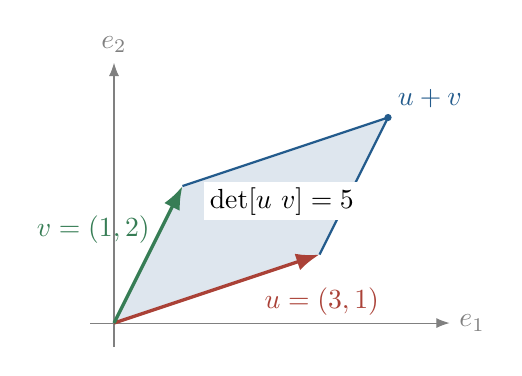
\begin{tikzpicture}[>=Latex,scale=0.87]
 \coordinate (O) at (0,0);
 \coordinate (U) at (3,1);
 \coordinate (V) at (1,2);
 \coordinate (UV) at (4,3);
 \fill[manifoldblue!15] (O)--(U)--(UV)--(V)--cycle;
 \draw[manifoldblue,thick] (U)--(UV)--(V);
 \draw[->,gray] (-0.35,0)--(4.9,0) node[right] {\(e_1\)};
 \draw[->,gray] (0,-0.35)--(0,3.8) node[above] {\(e_2\)};
 \draw[->,very thick,manifoldred] (O)--(U)
   node[pos=.68,below right] {\(u=(3,1)\)};
 \draw[->,very thick,manifoldgreen] (O)--(V)
   node[pos=.68,left] {\(v=(1,2)\)};
 \fill[manifoldblue] (UV) circle (1.5pt)
   node[above right] {\(u+v\)};
 \node[fill=white,inner sep=2pt] at (2.45,1.78)
   {\(\det[u\ v]=5\)};
\end{tikzpicture}
\caption{W \(\mathbb R^2\) iloczyn zewnętrzny
\(u\wedge v=5e_1\wedge e_2\)
koduje zorientowane pole równoległoboku.
Zmiana kolejności wektorów zmienia znak.}
\label{fig:lin11-wedge-pole}
\end{figure}

\section{Potęgi zewnętrzne dualu i formy naprzemienne}
\label{sec:lin11-dual-formy}

\begin{twierdzenie}[Formy naprzemienne jako elementy dualu]
\label{thm:lin11-formy-alt}
Niech \(V\) będzie przestrzenią
wektorową nad \(K\), a \(k\ge0\).
Istnieje kanoniczny izomorfizm
\[
 (\Lambda^k(V))^*
 \cong \operatorname{Alt}^k(V^*),
\]
gdzie prawa strona oznacza
przestrzeń naprzemiennych form
\(k\)-liniowych \(V^k\to K\)
z Rozdziału~\ref{ch:lin8-wieloliniowe}.
Jeśli ponadto \(\dim V<\infty\),
istnieje kanoniczny izomorfizm
\[
 \mathcal E_k\colon
 \Lambda^k(V^*)\longrightarrow
 \operatorname{Alt}^k(V^*)
\]
zadany dla \(k\ge1\) na
wielowektorach prostych wzorem
\[
 \mathcal E_k(\varphi_1\wedge\cdots\wedge\varphi_k)
 (v_1,\ldots,v_k)
 =\det(\varphi_a(v_b))_{a,b=1}^k.
\]
Dla \(k=0\) przyjmujemy
\(\mathcal E_0=\operatorname{id}_K\).
Oba izomorfizmy obowiązują
nad ciałem dowolnej charakterystyki.
\end{twierdzenie}
\begin{proof}
Dla \(k=0\) lewa strona pierwszego
izomorfizmu jest równa \(K^*\), a prawa
\(K\). W tym przypadku izomorfizm
jest dany przez ewaluację
\(L\mapsto L(1_K)\), której
odwrotnością jest
\(a\mapsto[x\mapsto ax]\).
Dla \(k\ge1\) funkcjonał
\(L\in(\Lambda^k(V))^*\)
wyznacza odwzorowanie
\[
 F_L(v_1,\ldots,v_k)
 :=L(v_1\wedge\cdots\wedge v_k),
\]
które jest \(k\)-liniowe
i naprzemienne.
Odwrotnie, dla każdej
naprzemiennej formy \(F\)
Twierdzenie~\ref{thm:lin11-potega-wedge-uniwersalna}
daje jednoznaczny funkcjonał
\(L_F\) spełniający
\(L_F(v_1\wedge\cdots\wedge v_k)
=F(v_1,\ldots,v_k)\).
Oba przyporządkowania są
liniowe i wzajemnie odwrotne,
ponieważ wielowektory proste
rozpinają \(\Lambda^k(V)\).

Załóżmy teraz \(\dim V=n<\infty\).
Dla \(\varphi_1,\ldots,\varphi_k\in V^*\)
wyznacznik z tezy jest
liniowy oddzielnie w każdym
\(\varphi_a\) i znika,
gdy dwa z nich są równe,
bo wtedy dwa wiersze są
identyczne.
Wobec tego własność uniwersalna
potęgi zewnętrznej \(V^*\)
daje dobrze określone liniowe
odwzorowanie \(\mathcal E_k\).
Wartości są naprzemiennymi
formami na \(V\), ponieważ
wyznacznik jest także
naprzemienny i wieloliniowy
w kolumnach.

Wybierzmy bazę
\(B=(e_1,\ldots,e_n)\)
i jej bazę dualną
\((e^1,\ldots,e^n)\).
Dla rosnących krotek \(I,J\)
długości \(k\) mamy
\[
 \mathcal E_k(
 e^{i_1}\wedge\cdots\wedge e^{i_k})
 (e_{j_1},\ldots,e_{j_k})
 =\det(\delta_{i_a j_b})
 =\delta_{I,J}.
\]
Oznacza to, że baza
\(\Lambda^k(V^*)\) z
Twierdzenia~\ref{thm:lin11-zew-baza}
przechodzi na bazę form
naprzemiennych opisaną w
Twierdzeniu~\ref{thm:lin8-wymiar-alt}.
Odwzorowanie jest zatem
izomorfizmem.
Dla \(k>n\) obie przestrzenie
są zerowe, a dla \(k=0\)
izomorfizm jest identycznością.
\end{proof}

\begin{wniosek}[Iloczyn zewnętrzny form — wzór z przetasowaniami]
\label{cor:lin11-shuffle}
Niech \(V\) będzie skończenie
wymiarową przestrzenią nad \(K\).
Niech \(p,q\in\mathbb N_0\),
\(\alpha\in\operatorname{Alt}^p(V^*)\),
\(\beta\in\operatorname{Alt}^q(V^*)\).
Przenosząc mnożenie z
\(\Lambda(V^*)\) przez izomorfizmy
\(\mathcal E_p,\mathcal E_q,
\mathcal E_{p+q}\), otrzymujemy
iloczyn zewnętrzny form
o wzorze
\[
 \begin{aligned}
 &(\alpha\wedge\beta)(v_1,\ldots,v_{p+q})\\
 &\quad=\sum_{\sigma\in\operatorname{Sh}(p,q)}
  \operatorname{sgn}(\sigma)
  \alpha(v_{\sigma(1)},\ldots,v_{\sigma(p)})
  \beta(v_{\sigma(p+1)},\ldots,v_{\sigma(p+q)}),
 \end{aligned}
\]
gdzie \(\operatorname{Sh}(p,q)\) jest
zbiorem permutacji \(\sigma\in S_{p+q}\)
spełniających
\(\sigma(1)<\cdots<\sigma(p)\) oraz
\(\sigma(p+1)<\cdots<\sigma(p+q)\).
Dla \(p=0\) lub \(q=0\)
prawa strona jest zwykłym
mnożeniem przez skalar.
Formuła nie zawiera dzielenia
przez silnie i obowiązuje
w dowolnej charakterystyce.
\end{wniosek}
\begin{proof}
Wystarczy udowodnić wzór
dla \(\alpha\) i \(\beta\)
pochodzących od prostych
iloczynów elementów \(V^*\):
takie elementy rozpinają
\(\Lambda^p(V^*)\) i
\(\Lambda^q(V^*)\), a oba
wyrażenia są dwuliniowe.
Niech
\(\alpha=\mathcal E_p(
 \varphi_1\wedge\cdots\wedge\varphi_p)\),
\(\beta=\mathcal E_q(
 \psi_1\wedge\cdots\wedge\psi_q)\).
Wtedy \(\alpha\wedge\beta\)
jest obrazem
\(\varphi_1\wedge\cdots\wedge\varphi_p
\wedge\psi_1\wedge\cdots\wedge\psi_q\),
więc jego wartość na
\((v_1,\ldots,v_{p+q})\)
jest wyznacznikiem macierzy
o pierwszych \(p\) wierszach
\(\varphi_a(v_b)\) i ostatnich
\(q\) wierszach \(\psi_c(v_b)\).
Rozwińmy ten wyznacznik
według pierwszych \(p\) wierszy.
Wybór \(p\) kolumn
indeksowanych rosnąco,
oraz rosnąco indeksowanych
pozostałych \(q\) kolumn,
jest równoważny wyborowi
przetasowania \(\sigma\).
Znak rozwinięcia jest równy
\(\operatorname{sgn}(\sigma)\).
Odpowiednie dwa minory
są dokładnie wartościami
\(\alpha\) i \(\beta\)
na wskazanych argumentach.
Otrzymujemy wzór z tezy
dla form prostych, a
dwuliniowość daje go dla
dowolnych \(\alpha,\beta\).
Rachunek wyznacznika i
rozwinięcie Laplace'a są
poprawne nad dowolnym ciałem.
\end{proof}

\begin{przyklad}[Kontrola współczynnika w iloczynie form]
\label{prz:lin11-shuffle}
Niech \(V=\mathbb R^3\)
z bazą \((e_1,e_2,e_3)\)
i dualną bazą \((e^1,e^2,e^3)\).
Weźmy
\(\alpha=\mathcal E_2(e^1\wedge e^2)\)
i \(\beta=\mathcal E_1(e^3)\).
Na krotce \((e_1,e_2,e_3)\)
z trzech przetasowań \((2,1)\)
jedynie identyczność wnosi
niezerowy składnik, równy \(1\).
Stąd
\[
 (\alpha\wedge\beta)(e_1,e_2,e_3)=1.
\]
Jest to także
\(\det I_3\), zgodnie z
\(\mathcal E_3(e^1\wedge e^2\wedge e^3)\).
W odróżnieniu od
nienormalizowanej sumy po
wszystkich \(3!\) permutacjach
nie pojawia się czynnik \(2!\).
\end{przyklad}

\section{Symetryzacja i alternowanie tensorów}
\label{sec:lin11-projekcje}

\begin{stwierdzenie}[Permutacje czynników tensorowych]
\label{prop:lin11-permutacje}
Niech \(k\ge1\).
Dla każdej \(\sigma\in S_k\)
istnieje dokładnie jedno liniowe
odwzorowanie
\(P_\sigma\colon V^{\otimes k}\to V^{\otimes k}\)
takie, że
\[
 P_\sigma(v_1\otimes\cdots\otimes v_k)
 =v_{\sigma^{-1}(1)}\otimes\cdots
  \otimes v_{\sigma^{-1}(k)}.
\]
Spełnia ono
\(P_\sigma P_\tau=P_{\sigma\tau}\).
Operatory
\[
 \mathcal S_k=\sum_{\sigma\in S_k}P_\sigma,
 \qquad
 \mathcal A_k=\sum_{\sigma\in S_k}
                \operatorname{sgn}(\sigma)P_\sigma
\]
są liniowe nad każdym ciałem.
Zachodzą
\[
 \mathcal S_k^2=k!\,\mathcal S_k,\qquad
 \mathcal A_k^2=k!\,\mathcal A_k.
\]
Jeżeli \(k!1_K\ne0_K\),
to \((k!)^{-1}\mathcal S_k\)
i \((k!)^{-1}\mathcal A_k\)
są rzutowaniami liniowymi.
\end{stwierdzenie}
\begin{proof}
Zadany wzór jest \(k\)-liniowy
w \(v_1,\ldots,v_k\).
Istnienie i jednoznaczność
\(P_\sigma\) wynikają z
Twierdzenia~\ref{thm:lin10-wielokrotny}.
Dla tensora prostego po
zastosowaniu najpierw \(P_\tau\),
a potem \(P_\sigma\),
na miejscu \(i\) stoi
\(v_{\tau^{-1}(\sigma^{-1}(i))}
=v_{(\sigma\tau)^{-1}(i)}\).
Otrzymujemy
\(P_\sigma P_\tau=P_{\sigma\tau}\)
na tensorach prostych, a więc
na całej przestrzeni.

W podwójnej sumie
\(\mathcal S_k^2\)
dla każdej permutacji
\(\rho\in S_k\) występuje
dokładnie \(k!\) par
\((\sigma,\tau)\) o \(\sigma\tau=\rho\).
Stąd \(\mathcal S_k^2=k!\mathcal S_k\).
Dla \(\mathcal A_k\) dodatkowy
współczynnik
\(\operatorname{sgn}(\sigma)
\operatorname{sgn}(\tau)
=\operatorname{sgn}(\rho)\)
daje ten sam wynik.
Gdy \(k!1_K\ne0_K\),
jest on odwracalny w ciele.
Podzielenie obu równości
przez \((k!)^2\) dowodzi
idempotencji znormalizowanych
operatorów.
\end{proof}

\begin{uwaga}[Dlaczego iloraz jest konstrukcją podstawową]
\label{rem:lin11-kchar}
Znormalizowana symetryzacja
i alternowanie stanowią
wygodne narzędzia, gdy
charakterystyka ciała nie dzieli \(k!\).
Jeśli \(k!1_K=0_K\),
wzory z dzieleniem przez \(k!\)
nie mają sensu.
Nie oznacza to jednak, że
\(S^k(V)\) lub \(\Lambda^k(V)\)
przestają istnieć:
obie przestrzenie są
zdefiniowane jako ilorazy
algebry tensorowej, bez
jakiegokolwiek dzielenia.
Rozdział~\ref{ch:lin8-wieloliniowe}
opisuje tę samą przeszkodę
dla operatorów działających
na formach wieloliniowych.
\end{uwaga}

\begin{stwierdzenie}[Symetryczny iloraz a symetryzator]
\label{prop:lin11-projekcje-ilorazy}
Niech \(k\ge1\) i załóżmy,
że \(k!1_K\ne0_K\).
Niech \(q_k^S\colon
V^{\otimes k}\to S^k(V)\)
i \(q_k^\Lambda\colon
V^{\otimes k}\to\Lambda^k(V)\)
będą naturalnymi odwzorowaniami
ilorazowymi.
Wówczas ograniczenia
\[
 \begin{aligned}
 q_k^S|_{\operatorname{im}((k!)^{-1}\mathcal S_k)}
 &\colon \operatorname{im}((k!)^{-1}\mathcal S_k)
       \longrightarrow S^k(V),\\
 q_k^\Lambda|_{\operatorname{im}((k!)^{-1}\mathcal A_k)}
 &\colon \operatorname{im}((k!)^{-1}\mathcal A_k)
       \longrightarrow \Lambda^k(V)
 \end{aligned}
\]
są izomorfizmami.
Są to dwa różne sposoby
opisania tych samych ilorazów,
dostępne przy wskazanym
założeniu o charakterystyce.
\end{stwierdzenie}
\begin{proof}
Oznaczmy znormalizowane operatory
przez \(P_S\) i \(P_\Lambda\).
Dla permutacji czynników
mamy
\(q_k^S P_\sigma=q_k^S\)
z przemienności w \(S(V)\)
oraz
\(q_k^\Lambda P_\sigma
=\operatorname{sgn}(\sigma)q_k^\Lambda\)
z reguły znaków.
Zatem po zsumowaniu
\[
 q_k^S P_S=q_k^S,\qquad
 q_k^\Lambda P_\Lambda=q_k^\Lambda.
\]
Te równości zapewniają
surjektywność obu ograniczeń:
każdy element ilorazu
ma przedstawiciela z obrazu
odpowiedniego rzutowania.

Wykażmy teraz, że
\(P_S\) zeruje jądro \(q_k^S\).
Ideał symetryczny w stopniu
\(k\) jest rozpięty przez
tensory postaci
\(x\otimes(u\otimes v-v\otimes u)\otimes y\),
z możliwymi pustymi czynnikami
\(x,y\). Dla każdej z takich
różnic dwie sumy po
wszystkich permutacjach
czynników są jednakowe,
więc ich różnica jest zerowa.
Z liniowości \(P_S\)
zeruje całe jądro.
Analogicznie
\(P_\Lambda\) zeruje jądro
\(q_k^\Lambda\):
dla tensora z dwoma
sąsiednimi równymi wektorami
składniki sumy alternującej
łączą się w pary,
które mają równe wartości
tensorowe i przeciwne znaki.
Nie wymaga to dzielenia
przez \(2\).
Każdy element jądra
jest kombinacją takich
tensorów z dwoma
równymi sąsiednimi czynnikami.

Jeśli \(x=P_S(t)\)
i \(q_k^S(x)=0\), to
\(P_S(x)=0\), ponieważ
\(x\in\ker q_k^S\).
Z drugiej strony
\(P_S(x)=P_S^2(t)=P_S(t)=x\).
Stąd \(x=0\).
Ten sam argument
z \(P_\Lambda\) wykazuje
iniektywność drugiego
ograniczenia. Oba są więc
izomorfizmami.
\end{proof}

\section{Podsumowanie}
\label{sec:lin11-podsumowanie}

Algebra tensorowa \(T(V)\)
łączy wszystkie potęgi
\(V^{\otimes k}\) i zachowuje
kolejność czynników.
Jej iloraz \(S(V)\) wymusza
przemienność i w skończonym
wymiarze jest izomorficzny
z algebrą wielomianów.
Iloraz \(\Lambda(V)\) wymusza
\(v\wedge v=0\) i daje
naprzemienne iloczyny zewnętrzne.
W skończonym wymiarze
potęgi zewnętrzne mają bazy
indeksowane rosnącymi krotkami
i wymiary \(\binom nk\).
Współczynniki
\(v_1\wedge\cdots\wedge v_k\)
są minorami macierzy kolumn,
a macierz \(\Lambda^k A\)
jest złożona z minorów
macierzy \(A\).
Przy \(k=\dim V\) działanie
na jednowymiarowej
\(\Lambda^k(V)\) jest mnożeniem
przez wyznacznik.
Własność uniwersalna
potęgi zewnętrznej
identyfikuje jej dual z
przestrzenią form naprzemiennych,
a iloczyn form otrzymuje
wzór z przetasowaniami,
poprawny nad każdym ciałem.
Symetryzatory i antysymetryzatory
są wygodnymi dodatkowymi
reprezentacjami ilorazów
tylko przy założeniu, że
\(k!\) jest odwracalne w \(K\).

\chapter{Przestrzenie euklidesowe i unitarne}
\label{ch:lin12-euklidesowe-unitarne}
\index{przestrzeń euklidesowa@Przestrzeń euklidesowa}
\index{przestrzeń unitarna@Przestrzeń unitarna}
\index{forma hermitowska@Forma hermitowska}
\index{iloczyn skalarny zespolony@Iloczyn skalarny zespolony}

\noindent\textbf{Cel rozdziału.}
W Rozdziale~\ref{ch:lin9-formy-kwadratowe} udowodniliśmy
podstawowe twierdzenia o rzeczywistych iloczynach skalarnych:
nierówność Cauchy'ego--Schwarza, ortogonalizację
Grama--Schmidta i istnienie rzutów ortogonalnych.
Nie będziemy powtarzać tych dowodów.
Rozszerzymy natomiast teorię na przestrzenie zespolone.
Właściwym odpowiednikiem rzeczywistej symetrycznej formy
dwuliniowej jest tam \emph{forma hermitowska}, która
w pierwszym argumencie jest sprzężenie liniowa,
a w drugim liniowa. Zbadamy polaryzację zespoloną,
współrzędne, nierówność Cauchy'ego--Schwarza,
bazy ortonormalne, reprezentację Riesza i
odwzorowania unitarne. W kolejnych rozdziałach
będziemy mogli dzięki temu badać bardziej szczegółowo
rzuty i operatory na przestrzeniach z iloczynem skalarnym.

Przez \(K\) oznaczamy \(\mathbb R\) albo \(\mathbb C\).
Symbol \(\overline a\) oznacza sprzężenie zespolone,
a dla \(K=\mathbb R\) przyjmujemy \(\overline a=a\).
Nie wymagamy skończonego wymiaru, o ile założenie
to nie jest wyraźnie wskazane. Przestrzenie są
algebraiczne; nie wprowadzamy tu pojęcia zupełności
przestrzeni unormowanej.

\section{Formy hermitowskie i iloczyny skalarne}
\label{sec:lin12-hermitowskie}

\begin{definicja}[Forma półtoraliniowa i hermitowska]
\label{def:lin12-hermitowska}
Niech \(V\) będzie przestrzenią wektorową nad \(K\).
Odwzorowanie \(h\colon V\times V\to K\)
nazywamy \emph{formą półtoraliniową}
(z konwencją liniowości w drugim argumencie),
jeśli dla wszystkich \(u,v,w\in V\)
oraz \(a,b\in K\) zachodzą
\[
 \begin{aligned}
 h(au+bv,w)&=\overline a\,h(u,w)+
              \overline b\,h(v,w),\\
 h(w,au+bv)&=a\,h(w,u)+b\,h(w,v).
 \end{aligned}
\]
Formę taką nazywamy \emph{hermitowską}, jeśli
\[
 h(v,u)=\overline{h(u,v)}
 \qquad(u,v\in V).
\]
Forma hermitowska jest \emph{dodatnio określona},
jeżeli \(h(v,v)>0\) dla każdego \(v\ne0_V\).
Wówczas nazywamy ją \emph{iloczynem skalarnym},
a parę \((V,h)\) \emph{przestrzenią euklidesową}
dla \(K=\mathbb R\) albo \emph{przestrzenią unitarną}
dla \(K=\mathbb C\).
\end{definicja}

\begin{uwaga}[Konwencja dotycząca argumentów]
\label{rem:lin12-konwencja}
W literaturze występuje też konwencja, w której
iloczyn skalarny jest liniowy w pierwszym,
a sprzężenie liniowy w drugim argumencie.
Nie wolno mieszać obu konwencji:
przy naszej definicji
\(h(u,av)=a\,h(u,v)\),
natomiast \(h(au,v)=\overline a\,h(u,v)\).
Wszystkie wzory na macierze, współrzędne,
polaryzację oraz reprezentację Riesza
są poniżej zgodne właśnie z tą konwencją.
\end{uwaga}

\begin{stwierdzenie}[Przekątna formy hermitowskiej]
\label{prop:lin12-przekatna}
Niech \(h\) będzie formą hermitowską na \(V\).
Wtedy \(h(v,v)\in\mathbb R\) dla każdego \(v\in V\).
Ponadto \(h(0_V,v)=h(v,0_V)=0_K\).
Jeżeli \(h\) jest dodatnio określona, to
\(h(v,v)=0\) zachodzi wyłącznie dla \(v=0_V\).
\end{stwierdzenie}
\begin{proof}
Z hermitowskości dla \(u=v\) otrzymujemy
\(h(v,v)=\overline{h(v,v)}\), więc
\(h(v,v)\) jest rzeczywista.
Półtoraliniowość daje
\(h(0_V,v)=0_K\) i \(h(v,0_V)=0_K\)
po podstawieniu skalaru \(0_K\).
Pozostała teza wynika bezpośrednio
z dodatniej określoności.
\end{proof}

\begin{przyklad}[Standardowy iloczyn skalarny]
\label{prz:lin12-standardowy}
Niech \(n\in\mathbb N_0\).
Na \(K^n\) określamy
\[
 h(z,w)=\sum_{j=1}^{n}\overline{z_j}w_j.
\]
Pierwszy argument jest sprzężenie liniowy,
a drugi liniowy. Zamiana argumentów
daje sprzężenie wartości całej sumy.
Ponadto
\(h(z,z)=\sum_j|z_j|^2\ge0\),
przy czym równość zachodzi dokładnie dla \(z=0\).
Otrzymujemy przestrzeń euklidesową
dla \(K=\mathbb R\) i unitarną
dla \(K=\mathbb C\).
Przy \(n=0\) jest to jedyny iloczyn
skalarny na przestrzeni zerowej;
warunek dodatniej określoności jest
spełniony w sposób pusty.
\end{przyklad}

\begin{przyklad}[Dlaczego zwykła dwuliniowość nie wystarcza]
\label{prz:lin12-nie-dwuliniowa}
Na \(\mathbb C\) funkcja \(b(z,w)=zw\)
jest dwuliniowa nad \(\mathbb C\),
ale nie jest dodatnio określonym
iloczynem skalarnym:
\(b(i,i)=-1\).
Ponadto \(b(1,i)=i=b(i,1)\),
podczas gdy hermitowskość wymagałaby
\(b(i,1)=\overline{b(1,i)}=-i\).
Poprawny iloczyn skalarny na \(\mathbb C\)
ma postać \(h(z,w)=\overline zw\).
\end{przyklad}

\section{Polaryzacja zespolona}
\label{sec:lin12-polaryzacja}

\begin{twierdzenie}[Tożsamość polaryzacyjna]
\label{thm:lin12-polaryzacja}
Niech \(h\colon V\times V\to\mathbb C\)
będzie formą hermitowską i
\(q(v):=h(v,v)\in\mathbb R\).
Wówczas dla wszystkich \(u,v\in V\)
\[
 \begin{aligned}
 h(u,v)=\frac14\bigl(
 &q(u+v)-q(u-v)\\
 &-i\,q(u+iv)+i\,q(u-iv)\bigr).
 \end{aligned}
\]
W szczególności dwie formy hermitowskie
na tej samej przestrzeni zespolonej,
które mają jednakowe wartości na przekątnej,
są równe. Dla \(K=\mathbb R\) odpowiedni wzór
ma postać
\[
 h(u,v)=\tfrac14\bigl(q(u+v)-q(u-v)\bigr).
\]
Nie trzeba zakładać dodatniej określoności.
\end{twierdzenie}
\begin{proof}
Niech \(z=h(u,v)\).
Z półtoraliniowości i hermitowskości
otrzymujemy
\[
 \begin{aligned}
 q(u+v)&=q(u)+q(v)+z+\overline z,\\
 q(u-v)&=q(u)+q(v)-z-\overline z.
 \end{aligned}
\]
Zatem różnica pierwszych dwóch wartości
wynosi \(2(z+\overline z)=4\operatorname{Re}z\).
Dla argumentów \(u\pm iv\) mamy
\[
 \begin{aligned}
 q(u+iv)&=q(u)+q(v)+iz-i\overline z,\\
 q(u-iv)&=q(u)+q(v)-iz+i\overline z.
 \end{aligned}
\]
Ich różnica jest równa
\(2i(z-\overline z)=-4\operatorname{Im}z\).
Wstawiając te dwie różnice do wzoru z tezy,
otrzymujemy
\(\operatorname{Re}z+i\operatorname{Im}z=z\).

Jeśli \(h_1(u,u)=h_2(u,u)\)
dla wszystkich \(u\), to zastosowanie
tego samego wzoru do obu form
daje \(h_1(u,v)=h_2(u,v)\)
dla wszystkich \(u,v\).
Dla \(K=\mathbb R\)
formy hermitowskie są symetrycznymi
formami dwuliniowymi, więc wystarczają
pierwsze dwie równości.
\end{proof}

\begin{przyklad}[Odzyskanie części urojonej]
\label{prz:lin12-polaryzacja-i}
Niech \(V=\mathbb C\) z iloczynem
\(h(z,w)=\overline zw\), a
\(q(z)=|z|^2\).
Dla \(u=1\), \(v=i\)
mamy \(h(1,i)=i\), lecz
\(q(1+i)=q(1-i)=2\).
Rzeczywista różnica kwadratów jest zerowa.
Natomiast
\(q(1+i\cdot i)=q(0)=0\)
i \(q(1-i\cdot i)=q(2)=4\).
Tożsamość polaryzacyjna daje
\(\frac14(0-i(0-4))=i\),
zgodnie z wartością iloczynu skalarnego.
Zastosowanie wyłącznie rzeczywistego
wzoru polaryzacyjnego prowadziłoby
do błędnego wyniku \(0\).
\end{przyklad}

\section{Macierz Grama i zmiana bazy}
\label{sec:lin12-gram}

\begin{definicja}[Macierz Grama]
\label{def:lin12-gram}
Niech \(\dim V=n<\infty\), a
\(B=(e_1,\ldots,e_n)\) będzie
uporządkowaną bazą \(V\).
Dla formy hermitowskiej \(h\)
\emph{macierzą Grama} nazywamy
\[
 G_B(h)=(h(e_i,e_j))_{i,j=1}^{n}.
\]
Dla macierzy \(A\) symbol \(A^*\)
oznacza macierz sprzężoną i transponowaną,
tj. \((A^*)_{ij}=\overline{A_{ji}}\).
Macierz \(A\) jest \emph{hermitowska},
jeżeli \(A^*=A\).
\end{definicja}

\begin{twierdzenie}[Współrzędne i kongruencja hermitowska]
\label{thm:lin12-gram-zmiana}
Niech \(V\) będzie skończenie wymiarową
przestrzenią nad \(K\),
\(h\) formą hermitowską oraz
\(B=(e_1,\ldots,e_n)\) bazą.
Wtedy macierz \(G=G_B(h)\)
jest hermitowska, a dla
\(X=[u]_B\), \(Y=[v]_B\) zachodzi
\[
 h(u,v)=X^*GY.
\]
Odwrotnie, każda macierz hermitowska
\(G\in\operatorname{Mat}_{n\times n}(K)\)
definiuje w ten sposób jednoznaczną
formę hermitowską na \(K^n\).
Jeżeli baza \(B'\) jest wyrażona
w bazie \(B\) macierzą przejścia \(P\),
czyli \([v]_B=P[v]_{B'}\), to
\[
 G_{B'}(h)=P^*G_B(h)P.
\]
Forma \(h\) jest dodatnio określona
dokładnie wtedy, gdy
\(X^*GX>0\) dla wszystkich \(X\ne0\).
\end{twierdzenie}
\begin{proof}
Dla \(G_{ij}=h(e_i,e_j)\)
hermitowskość daje
\(G_{ji}=\overline{G_{ij}}\),
co jest równoważne \(G^*=G\).
Pisząc
\(u=\sum_i x_ie_i\), \(v=\sum_j y_je_j\),
stosujemy półtoraliniowość:
\[
 h(u,v)=\sum_{i,j}\overline{x_i}\,
         h(e_i,e_j)y_j=X^*GY.
\]
Jeśli \(G^*=G\), to
\(h_G(X,Y)=X^*GY\)
jest sprzężenie liniowe w \(X\)
i liniowe w \(Y\), a ponadto
\[
 \overline{h_G(Y,X)}
 =\overline{Y^*GX}
 =X^*G^*Y=X^*GY.
\]
Zatem \(h_G\) jest hermitowska.
Jednoznaczność wynika z jej wartości
na parach wektorów bazowych.
W nowej bazie
\(X=P X'\), \(Y=P Y'\),
więc
\(X^*GY=(X')^*P^*GPY'\);
to daje wzór kongruencji.
Ostatnia równoważność jest dokładnie
definicją dodatniej określoności
w nieosobliwym układzie współrzędnych.
\end{proof}

\begin{przyklad}[Niediagonalna macierz hermitowska]
\label{prz:lin12-gram-i}
Niech na \(\mathbb C^2\) zadana będzie
macierz
\[
 G=\begin{pmatrix}2&i\\-i&2\end{pmatrix}.
\]
Jest hermitowska, bo \(G^*=G\),
ale nie jest macierzą rzeczywistą.
Odpowiadająca jej forma ma
na przekątnej wartość
\[
 q(z)=2|z_1|^2+2|z_2|^2
       -2\operatorname{Im}(\overline{z_1}z_2).
\]
Po uzupełnieniu kwadratu
\[
 q(z)=2\left|z_1+\frac i2z_2\right|^2
       +\frac32|z_2|^2.
\]
Oba składniki są nieujemne,
a ich suma znika wyłącznie
dla \(z_1=z_2=0\).
Forma jest zatem dodatnio określona.
Z tego samego rozkładu wynika,
dlaczego hermitowskość \(G\)
nie wystarcza sama w sobie
do dodatniej określoności:
np. macierz \(\operatorname{diag}(1,-1)\)
jest hermitowska, lecz nie jest
dodatnio określona.
\end{przyklad}

\section{Nierówność Cauchy'ego--Schwarza i norma}
\label{sec:lin12-norma}

\begin{twierdzenie}[Nierówność Cauchy'ego--Schwarza nad \(\mathbb C\)]
\label{thm:lin12-cauchy-schwarz}
Niech \((V,h)\) będzie przestrzenią unitarną.
Dla dowolnych \(u,v\in V\) mamy
\[
 |h(u,v)|^2\le h(u,u)\,h(v,v).
\]
Równość zachodzi dokładnie wtedy,
gdy \(u,v\) są liniowo zależne nad \(\mathbb C\).
Funkcja
\(\|v\|:=\sqrt{h(v,v)}\)
jest normą na \(V\), a
\[
 \|u+v\|\le\|u\|+\|v\|.
\]
\end{twierdzenie}
\begin{proof}
Jeżeli \(v=0_V\), nierówność
jest równością i oba wektory
są liniowo zależne.
Niech więc \(v\ne0_V\).
Liczba \(h(v,v)\) jest dodatnia.
Kładziemy
\(c:=h(v,u)/h(v,v)\).
Wówczas
\(h(v,u-cv)=h(v,u)-c\,h(v,v)=0\).
Z nieujemności kwadratu normy
otrzymujemy
\[
 \begin{aligned}
 0&\le h(u-cv,u-cv)\\
  &=h(u,u)-\frac{|h(u,v)|^2}{h(v,v)}.
 \end{aligned}
\]
Pomnożenie przez \(h(v,v)>0\)
daje żądaną nierówność.
Równość jest równoważna
\(h(u-cv,u-cv)=0\),
czyli \(u=cv\).
W przypadku \(v=0\)
warunek zależności również zachodzi.

Dodatnia określoność daje
nieujemność \(\|v\|\) i
\(\|v\|=0\iff v=0\).
Półtoraliniowość zapewnia
\[
 \|av\|^2=h(av,av)=|a|^2 h(v,v),
\]
więc \(\|av\|=|a|\|v\|\).
Wreszcie
\[
 \begin{aligned}
 \|u+v\|^2
 &=\|u\|^2+2\operatorname{Re}h(u,v)+\|v\|^2\\
 &\le \|u\|^2+2|h(u,v)|+\|v\|^2\\
 &\le (\|u\|+\|v\|)^2.
 \end{aligned}
\]
Obie strony są nieujemne,
więc pierwiastkowanie daje
nierówność trójkąta.
\end{proof}

\begin{wniosek}[Wzór Pitagorasa i równoległoboku]
\label{cor:lin12-pitagoras}
Niech \((V,h)\) będzie przestrzenią
euklidesową lub unitarną.
Jeśli \(h(u,v)=0\), to
\[
 \|u+v\|^2=\|u\|^2+\|v\|^2.
\]
Dla dowolnych \(u,v\in V\) zachodzi
\[
 \|u+v\|^2+\|u-v\|^2
 =2\|u\|^2+2\|v\|^2.
\]
\end{wniosek}
\begin{proof}
Rozwijamy kwadraty norm za pomocą
półtoraliniowości. W pierwszym
przypadku oba mieszane składniki
\(h(u,v)\) i \(h(v,u)\) znikają.
W drugim przypadku składniki
mieszane w dwóch rozwinięciach
są przeciwne i znoszą się po dodaniu.
\end{proof}

\section{Bazy ortonormalne w przestrzeniach unitarnych}
\label{sec:lin12-bazy}

\begin{definicja}[Rodzina ortonormalna]
\label{def:lin12-ortonormalna}
W przestrzeni \((V,h)\) rodzinę
\((e_j)_{j\in J}\) nazywamy
\emph{ortonormalną}, jeśli
\(h(e_i,e_j)=\delta_{ij}\)
dla wszystkich \(i,j\in J\).
Jeśli jest bazą Hamela,
nazywamy ją \emph{bazą ortonormalną}.
\end{definicja}

\begin{twierdzenie}[Ortogonalizacja Grama--Schmidta nad \(\mathbb C\)]
\label{thm:lin12-gram-schmidt}
Niech \((V,h)\) będzie przestrzenią
unitarną, a \(v_1,\ldots,v_m\in V\),
\(m\ge0\), wektorami liniowo niezależnymi.
Istnieje rodzina ortonormalna
\(e_1,\ldots,e_m\), dla której
\[
 \operatorname{span}\{e_1,\ldots,e_j\}
 =\operatorname{span}\{v_1,\ldots,v_j\}
 \qquad(1\le j\le m).
\]
Można ją skonstruować wzorami
\[
 w_j=v_j-\sum_{\ell=1}^{j-1}
            h(e_\ell,v_j)e_\ell,
 \qquad
 e_j=\frac{w_j}{\sqrt{h(w_j,w_j)}}.
\]
W szczególności każda skończenie
wymiarowa przestrzeń unitarna
posiada bazę ortonormalną.
\end{twierdzenie}
\begin{proof}
Dla \(m=0\) rodzina pusta
spełnia tezę. Dla \(m\ge1\)
przeprowadzamy indukcję.
Przy \(j=1\) wektor \(v_1\)
jest niezerowy i normalizujemy go.
Załóżmy, że
\(e_1,\ldots,e_{j-1}\)
są ortonormalne i
rozpinają tę samą przestrzeń,
co \(v_1,\ldots,v_{j-1}\).
Dla każdego \(i<j\)
półtoraliniowość w drugim
argumencie daje
\[
 \begin{aligned}
 h(e_i,w_j)
 &=h(e_i,v_j)
   -\sum_{\ell<j}h(e_\ell,v_j)h(e_i,e_\ell)\\
 &=h(e_i,v_j)-h(e_i,v_j)=0.
 \end{aligned}
\]
Jeśli \(w_j=0\), to \(v_j\)
jest kombinacją poprzednich \(e_i\),
a zatem i poprzednich \(v_i\),
wbrew niezależności.
Dlatego \(h(w_j,w_j)>0\)
i wzór na \(e_j\) ma sens.
Nowy wektor jest normy \(1\)
i ortogonalny do poprzednich.
Ponadto \(w_j-v_j\) należy
do poprzedniej rozpiętości,
więc obie rodziny mają
taką samą rozpiętość do kroku \(j\).
Indukcja kończy konstrukcję.
Przy skończonym wymiarze
stosujemy ją do dowolnej bazy.
\end{proof}

\begin{przyklad}[Ortonormalizacja dwóch wektorów zespolonych]
\label{prz:lin12-gs-c2}
W \(\mathbb C^2\) ze standardowym
iloczynem skalarnym rozważmy
\(v_1=(1,i)\), \(v_2=(1,0)\).
Pierwszy wektor ortonormalny to
\[
 e_1=\frac1{\sqrt2}(1,i).
\]
Ponieważ
\(h(e_1,v_2)=1/\sqrt2\),
otrzymujemy
\[
 w_2=v_2-\tfrac1{\sqrt2}e_1
    =\bigl(\tfrac12,-\tfrac i2\bigr),
 \qquad
 e_2=\tfrac1{\sqrt2}(1,-i).
\]
Sprawdzenie bezpośrednie daje
\(h(e_1,e_2)=(1+(-i)(-i))/2=0\)
i \(h(e_2,e_2)=1\).
W tym rachunku sprzężenie
w pierwszym argumencie
jest istotne: zwykły iloczyn
współrzędnych nie dałby zera.
\end{przyklad}

\chapter{Ortogonalność i rzuty}
\label{ch:lin13-ortogonalnosc-rzuty}
\index{rzut ortogonalny@Rzut ortogonalny}
\index{dopełnienie ortogonalne@Dopełnienie ortogonalne}
\index{przybliżenie najlepsze@Przybliżenie najlepsze}
\index{równania normalne@Równania normalne}
\index{operator sprzężony@Operator sprzężony}

\noindent\textbf{Cel rozdziału.}
W Rozdziale~\ref{ch:lin9-formy-kwadratowe}
poznaliśmy dopełnienia ortogonalne dla rzeczywistych
form symetrycznych i udowodniliśmy istnienie rzutów
na podprzestrzenie w przestrzeniach euklidesowych.
W Rozdziale~\ref{ch:lin12-euklidesowe-unitarne}
rozszerzyliśmy iloczyny skalarne na ciało zespolone,
udowodniliśmy ortogonalizację i reprezentację Riesza.
Nie powtarzamy tych dowodów.
Celem obecnego rozdziału jest opis projekcji za pomocą
\emph{operatorów i macierzy}, rozwiązywanie problemu
najlepszego przybliżenia, równania normalne i
metoda najmniejszych kwadratów.
Wprowadzimy też operator sprzężony jako narzędzie
porządkujące wszystkie te konstrukcje.

Przez \(K\) oznaczamy \(\mathbb R\) lub \(\mathbb C\).
Przestrzenie \((V,h_V)\), \((W,h_W)\)
mają dodatnio określone iloczyny skalarne,
liniowe w \emph{drugim} argumencie:
\(h_V(au,v)=\overline a\,h_V(u,v)\),
\(h_V(u,av)=a h_V(u,v)\).
Wymiar skończony zakładamy tam, gdzie jest potrzebny,
a nie bez uzasadnienia dla całego rozdziału.
W bazach ortonormalnych zapisujemy macierze
przez \(A^*\), czyli sprzężenie transpozycję.

\section{Dopełnienia ortogonalne nad \(\mathbb R\) i \(\mathbb C\)}
\label{sec:lin13-dopelnienia}

\begin{definicja}[Dopełnienie ortogonalne]
\label{def:lin13-dopelnienie}
Niech \((V,h)\) będzie przestrzenią euklidesową
lub unitarną, a \(U\subseteq V\) podprzestrzenią.
Definiujemy
\[
 U^\perp=\{v\in V:\ h(u,v)=0
                     \text{ dla wszystkich }u\in U\}.
\]
Z hermitowskości wynika równoważność
\(h(u,v)=0\iff h(v,u)=0\);
kolejność argumentów w definicji
nie zmienia więc podprzestrzeni.
\end{definicja}

\begin{stwierdzenie}[Algebra dopełnień ortogonalnych]
\label{prop:lin13-dopelnienia}
Niech \((V,h)\) będzie przestrzenią
euklidesową lub unitarną.
Dla dowolnych podprzestrzeni
\(U,U_1,U_2\subseteq V\) mamy
\[
 \begin{gathered}
 U^\perp\text{ jest podprzestrzenią},\qquad
 U\cap U^\perp=\{0\},\qquad
 U\subseteq (U^\perp)^\perp,\\
 U_1\subseteq U_2\Longrightarrow
     U_2^\perp\subseteq U_1^\perp,\\
 (U_1+U_2)^\perp=U_1^\perp\cap U_2^\perp.
 \end{gathered}
\]
Nie zakładamy skończonego wymiaru.
\end{stwierdzenie}
\begin{proof}
Dla każdego \(u\in U\) odwzorowanie
\(v\mapsto h(u,v)\) jest liniowe,
więc \(U^\perp\) jest przecięciem
jąder odwzorowań liniowych.
Jeśli \(v\in U\cap U^\perp\),
to \(h(v,v)=0\); dodatnia określoność
daje \(v=0\).
Jeżeli \(u\in U\) i \(v\in U^\perp\),
to z hermitowskości
\(h(v,u)=\overline{h(u,v)}=0\),
skąd \(u\in(U^\perp)^\perp\).
Przy \(U_1\subseteq U_2\)
każdy wektor ortogonalny do \(U_2\)
jest ortogonalny do \(U_1\).

Jeśli \(v\in(U_1+U_2)^\perp\),
jest ortogonalny do każdego
elementu obu składników,
ponieważ \(U_i\subseteq U_1+U_2\).
Odwrotnie, dla
\(v\in U_1^\perp\cap U_2^\perp\)
i \(u_1\in U_1,u_2\in U_2\)
liniowość w pierwszym argumencie
z odpowiednim sprzężeniem daje
\(h(u_1+u_2,v)=0\).
Stąd obie strony ostatniej
równości są równe.
\end{proof}

\begin{twierdzenie}[Rozkład względem podprzestrzeni skończonego wymiaru]
\label{thm:lin13-rozklad}
Niech \((V,h)\) będzie przestrzenią
euklidesową lub unitarną,
niekoniecznie skończenie wymiarową.
Niech \(U\subseteq V\) będzie
podprzestrzenią \emph{skończonego wymiaru}.
Wtedy istnieje jednoznaczny rozkład
\[
 v=u+w,\qquad u\in U,\ w\in U^\perp,
 \quad\text{dla każdego }v\in V,
\]
czyli \(V=U\oplus U^\perp\).
Ponadto
\[
 (U^\perp)^\perp=U.
\]
W szczególności jeśli \(\dim V=n<\infty\),
to dla dowolnego \(U\subseteq V\)
zachodzi
\(\dim U^\perp=n-\dim U\).
\end{twierdzenie}
\begin{proof}
Wybierzmy ortonormalną bazę
\((e_1,\ldots,e_r)\) przestrzeni \(U\).
Jej istnienie w przypadku zespolonym
zapewnia
Twierdzenie~\ref{thm:lin12-gram-schmidt},
a w rzeczywistym
Twierdzenie~\ref{thm:lin9-gram-schmidt}.
Dla \(v\in V\) połóżmy
\[
 u=\sum_{j=1}^r h(e_j,v)e_j,
 \qquad w=v-u.
\]
Wtedy \(u\in U\), a dla każdego \(i\)
\[
 h(e_i,w)
 =h(e_i,v)-\sum_j h(e_j,v)h(e_i,e_j)=0.
\]
Ponieważ \(e_i\) rozpinają \(U\),
otrzymujemy \(w\in U^\perp\).
Jeśli \(v=u_1+w_1=u_2+w_2\)
są dwa takie rozkłady, to
\(u_1-u_2=w_2-w_1\)
należy do \(U\cap U^\perp=\{0\}\),
więc \(u_1=u_2\) i \(w_1=w_2\).

Dowiedliśmy już
\(U\subseteq(U^\perp)^\perp\).
Jeśli \(z\in(U^\perp)^\perp\),
piszemy \(z=u+w\) jak wyżej.
Wektor \(w\in U^\perp\), zatem
\(h(w,z)=0\); jednocześnie
\(h(w,u)=0\). Stąd
\(0=h(w,z)=h(w,u+w)=h(w,w)\),
więc \(w=0\), czyli \(z=u\in U\).
To dowodzi równości podprzestrzeni.
Dla skończenie wymiarowego \(V\)
rozmiar sumy prostej daje
\(\dim V=\dim U+\dim U^\perp\).
Przy \(U=\{0\}\) podane sumy są puste,
\(U^\perp=V\), i wszystkie wnioski
nadal zachodzą.
\end{proof}

\begin{uwaga}[Zakres twierdzenia o rozkładzie]
\label{rem:lin13-nieskonczony}
Skończony wymiar podprzestrzeni \(U\)
jest tu istotnym, wystarczającym założeniem;
nie wyciągamy z dowodu wniosku
\(V=U\oplus U^\perp\) dla \emph{dowolnej}
podprzestrzeni nieskończenie wymiarowej
w przestrzeni z iloczynem skalarnym.
Dla przestrzeni Hilberta istnieje
szersze twierdzenie dotyczące
podprzestrzeni domkniętych,
lecz wymaga ono topologii i zupełności.
Obecny dowód używa wyłącznie
skończonej bazy ortonormalnej \(U\).
\end{uwaga}

\section{Operator rzutu ortogonalnego}
\label{sec:lin13-projekcja}

\begin{definicja}[Rzut na podprzestrzeń]
\label{def:lin13-rzut}
Niech \(U\subseteq V\) będzie
skończenie wymiarową podprzestrzenią
przestrzeni euklidesowej lub unitarnej.
\emph{Rzutem ortogonalnym na \(U\)}
nazywamy odwzorowanie
\(P_U\colon V\to V\) przyporządkowujące
wektorowi \(v\) składnik \(u\in U\)
jego rozkładu \(v=u+w\),
\(w\in U^\perp\), z
Twierdzenia~\ref{thm:lin13-rozklad}.
\end{definicja}

\begin{twierdzenie}[Wzory na rzut i jego jądro]
\label{thm:lin13-rzut-wlasnosci}
Niech \((V,h)\) będzie przestrzenią
euklidesową lub unitarną, a
\(U\subseteq V\) podprzestrzenią
skończonego wymiaru.
Wtedy \(P_U\) jest liniowe i
\[
 \begin{gathered}
 \operatorname{im}P_U=U,\qquad
 \ker P_U=U^\perp,\qquad
 P_U^2=P_U,\\
 h(P_Uv,w)=h(v,P_Uw)
 \quad(v,w\in V).
 \end{gathered}
\]
Jeśli \((e_1,\ldots,e_r)\)
jest bazą ortonormalną \(U\), to
\[
 P_Uv=\sum_{j=1}^r h(e_j,v)e_j.
\]
Rzut \(P_U\) nie zależy od
wyboru bazy ortonormalnej \(U\).
Rzut \(I_V-P_U\) ma obraz \(U^\perp\)
i jądro \(U\), niezależnie
od wymiaru \(U^\perp\).
\end{twierdzenie}
\begin{proof}
Liniowość wynika wprost
z liniowości współczynników
\(h(e_j,v)\) w drugim argumencie.
Z
Twierdzenia~\ref{thm:lin13-rozklad}
podany wzór wybiera dokładnie
składnik należący do \(U\).
Jeśli \(u\in U\), to rozkład
\(u=u+0\) daje \(P_Uu=u\),
więc obraz to \(U\) i
\(P_U^2v=P_Uv\).
Równocześnie \(P_Uv=0\)
dokładnie wtedy, gdy \(v\in U^\perp\),
zatem \(\ker P_U=U^\perp\).

Dla \(v=u_v+w_v\) i
\(w=u_w+w_w\) z \(u_v,u_w\in U\)
i \(w_v,w_w\in U^\perp\) mamy
\[
 h(P_Uv,w)=h(u_v,u_w)
          =h(v,P_Uw).
\]
Jednoznaczność rozkładu
gwarantuje niezależność \(P_U\)
od użytej bazy.
Odwzorowanie \(I_V-P_U\)
przyporządkowuje \(v\)
składnik \(w_v\), więc ma
obraz \(U^\perp\), jądro \(U\)
i jest idempotentne.
\end{proof}

\begin{twierdzenie}[Najlepsze przybliżenie]
\label{thm:lin13-najlepsze}
Niech \((V,h)\) będzie
przestrzenią euklidesową lub unitarną,
a \(U\subseteq V\) podprzestrzenią
skończonego wymiaru.
Dla każdego \(v\in V\)
i \(u\in U\) zachodzi
\[
 \|v-u\|^2
 =\|v-P_Uv\|^2+\|P_Uv-u\|^2.
\]
Zatem \(P_Uv\) jest jedynym
punktem podprzestrzeni \(U\)
minimalizującym odległość do \(v\).
Dokładniej,
\[
 \operatorname{dist}(v,U)
 :=\inf_{u\in U}\|v-u\|
 =\|v-P_Uv\|.
\]
\end{twierdzenie}
\begin{proof}
Z własności rzutu
\(v-P_Uv\in U^\perp\).
Dla \(u\in U\) mamy też
\(P_Uv-u\in U\), więc te
dwa wektory są ortogonalne.
Z
Wniosku~\ref{cor:lin12-pitagoras}
otrzymujemy wskazaną równość.
Ostatni składnik jest nieujemny
i znika dokładnie wtedy,
gdy \(u=P_Uv\).
Wobec tego minimum jest
osiągane właśnie w \(P_Uv\)
i nigdzie indziej.
Równość dla odległości
wynika z wyciągnięcia
pierwiastków z równości norm.
\end{proof}

\begin{stwierdzenie}[Kontrakcja i optymalny rozkład normy]
\label{prop:lin13-kontrakcja}
Niech \(P_U\) będzie rzutem
ortogonalnym na skończenie
wymiarową podprzestrzeń
przestrzeni euklidesowej
lub unitarnej \(V\).
Dla każdego \(v\in V\) zachodzi
\[
 \|P_Uv\|\le\|v\|,\qquad
 \|(I_V-P_U)v\|\le\|v\|,
 \qquad
 \|v\|^2=\|P_Uv\|^2+
             \|(I_V-P_U)v\|^2.
\]
Jeżeli \(U\ne\{0\}\), to
\(\sup_{v\ne0}\|P_Uv\|/\|v\|=1\).
Jeśli \(U=\{0\}\), to \(P_U=0\).
\end{stwierdzenie}
\begin{proof}
Z rozkładu ortogonalnego
\(v=P_Uv+(I_V-P_U)v\)
wynika wzór Pitagorasa.
Oba kwadraty norm są
nieujemne, co daje obie
nierówności. Jeśli
\(U\ne\{0\}\), wybieramy
\(0\ne u\in U\). Ponieważ
\(P_Uu=u\), iloraz norm
jest równy \(1\), a
nie może przekraczać \(1\).
Dla \(U=\{0\}\) obraz rzutu
jest zerowy, więc rzut
jest odwzorowaniem zerowym.
\end{proof}

\begin{przyklad}[Rzut na prostą i hiperpłaszczyznę]
\label{prz:lin13-prosta}
Niech \(V=K^n\) ze standardowym
iloczynem skalarnym i niech \(a\in K^n\)
będzie niezerowy. Rzut na prostą
\(U=\operatorname{span}\{a\}\) ma postać
\[
 P_Uv=\frac{a^*v}{a^*a}\,a.
\]
Wynika to z wyboru
\(e=a/\sqrt{a^*a}\)
i wzoru na rzut w bazie
ortonormalnej \((e)\).
Dla hiperpłaszczyzny
\(H=a^\perp=\{v:a^*v=0\}\)
otrzymujemy
\[
 P_Hv=v-\frac{a^*v}{a^*a}\,a.
\]
Są to wzory poprawne także
nad \(\mathbb C\), ponieważ
\(a^*v\), a nie \(a^{\mathsf T}v\),
jest współczynnikiem rzutu.
\end{przyklad}

\begin{figure}[!htbp]
\centering
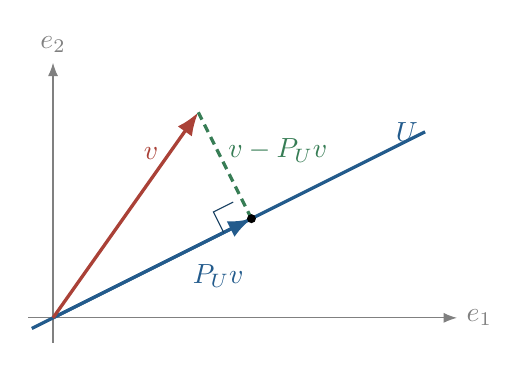
\begin{tikzpicture}[>=Latex,scale=.9]
 \draw[->,gray] (-0.35,0)--(5.7,0)
   node[right] {\(e_1\)};
 \draw[->,gray] (0,-0.35)--(0,3.6)
   node[above] {\(e_2\)};
 \draw[manifoldblue,very thick] (-.3,-.15)--(5.25,2.625);
 \node[manifoldblue,above right] at (4.7,2.35) {\(U\)};
 \coordinate (O) at (0,0);
 \coordinate (P) at (2.8,1.4);
 \coordinate (V) at (2.05,2.9);
 \draw[->,very thick,manifoldblue] (O)--(P)
    node[pos=.65,below right] {\(P_Uv\)};
 \draw[->,very thick,manifoldred] (O)--(V)
    node[pos=.80,left] {\(v\)};
 \draw[densely dashed,very thick,manifoldgreen] (P)--(V)
    node[pos=.64,right] {\(v-P_Uv\)};
 \draw[manifoldblue!70!black] ($(P)!0.14!(O)$)
   -- ++(-.145,.29) -- ++(.28,.14);
 \fill (P) circle (1.8pt);
\end{tikzpicture}
\caption{Rzut ortogonalny \(P_Uv\) i reszta
\(v-P_Uv\), prostopadła do podprzestrzeni \(U\).
Wektor \(P_Uv\) jest najlepszym
przybliżeniem \(v\) w \(U\).}
\label{fig:lin13-rzut-geometryczny}
\end{figure}


\section{Operator sprzężony i rzutowanie w skończonym wymiarze}
\label{sec:lin13-operator-sprzezony}

\begin{twierdzenie}[Istnienie operatora sprzężonego]
\label{thm:lin13-adjoint}
Niech \((V,h_V)\), \((W,h_W)\)
będą skończenie wymiarowymi
przestrzeniami euklidesowymi
lub unitarnymi nad tym samym ciałem \(K\).
Dla każdego odwzorowania liniowego
\(A\colon V\to W\)
istnieje dokładnie jedno liniowe
\(A^*\colon W\to V\), zwane
\emph{operatorem sprzężonym},
dla którego
\[
 h_W(Av,w)=h_V(v,A^*w)
 \qquad(v\in V,\ w\in W).
\]
W bazach ortonormalnych \(V,W\)
macierz operatora \(A^*\) jest
sprzężoną transpozycją macierzy \(A\).
\end{twierdzenie}
\begin{proof}
Ustalmy \(w\in W\).
Odwzorowanie
\[
 F_w\colon V\to K,\qquad
 F_w(v)=h_W(w,Av)
\]
jest liniowe względem \(v\),
ponieważ \(A\) jest liniowe,
a \(h_W\) jest liniowe
w drugim argumencie.
Z
Twierdzenia~\ref{thm:lin12-riesz}
istnieje dokładnie jeden
wektor \(a_w\in V\) taki, że
\[
 h_V(a_w,v)=h_W(w,Av)
 \qquad(v\in V).
\]
Po sprzężeniu obu stron
otrzymujemy
\[
 h_V(v,a_w)=h_W(Av,w).
\]
Określamy \(A^*w=a_w\).
Pozostaje sprawdzić liniowość.
Dla \(\lambda,\mu\in K\)
i \(w_1,w_2\in W\)
mamy dla każdego \(v\in V\)
\[
 \begin{aligned}
 h_V(v,A^*(\lambda w_1+\mu w_2))
 &=h_W(Av,\lambda w_1+\mu w_2)\\
 &=\lambda h_W(Av,w_1)+
   \mu h_W(Av,w_2)\\
 &=h_V(v,\lambda A^*w_1+\mu A^*w_2).
 \end{aligned}
\]
Podstawiając za \(v\)
różnicę dwóch wektorów
w drugim argumencie,
z dodatniej określoności
uzyskujemy ich równość.
Stąd \(A^*\) jest liniowe.
Ten sam argument dowodzi
jego jednoznaczności.

Niech teraz
\((e_1,\ldots,e_n)\),
\((f_1,\ldots,f_m)\)
będą bazami ortonormalnymi
\(V,W\), a \(M=[A]\).
Wtedy \([Av]=MX\),
\([w]=Y\) i
\[
 h_W(Av,w)=(MX)^*Y=X^*M^*Y.
\]
Z drugiej strony
\(h_V(v,A^*w)=X^*[A^*]Y\).
Równość dla wszystkich
\(X,Y\) daje \([A^*]=M^*\).
Przy wymiarze \(0\)
odwzorowania między odpowiednimi
przestrzeniami są jednoznaczne,
więc teza również obowiązuje.
\end{proof}

\begin{stwierdzenie}[Rachunek operatorów sprzężonych]
\label{prop:lin13-adjoint-kalkul}
Niech \(V,W,Z\) będą
skończenie wymiarowymi
przestrzeniami euklidesowymi
lub unitarnymi nad \(K\),
a \(A,B\colon V\to W\),
\(C\colon W\to Z\) odwzorowaniami liniowymi.
Dla dowolnych \(\lambda,\mu\in K\)
zachodzą
\[
 \begin{gathered}
 (\lambda A+\mu B)^*
   =\overline\lambda A^*+
    \overline\mu B^*,\\
 (C\circ A)^*=A^*\circ C^*,\qquad
 (A^*)^*=A,\qquad
 (I_V)^*=I_V.
 \end{gathered}
\]
Ponadto dla każdego \(v\in V\)
\[
 h_V(v,A^*Av)=h_W(Av,Av)\ge0.
\]
\end{stwierdzenie}
\begin{proof}
Dla pierwszego wzoru
stosujemy sprzężenie liniowość
pierwszego argumentu:
\[
 \begin{aligned}
 h_W((\lambda A+\mu B)v,w)
 &=\overline\lambda\,h_W(Av,w)
   +\overline\mu\,h_W(Bv,w)\\
 &=h_V(v,(\overline\lambda A^*+
                   \overline\mu B^*)w).
 \end{aligned}
\]
Jednoznaczność sprzężenia daje
pierwszą tożsamość.
Dla złożenia mamy
\[
 h_Z(CAv,z)
 =h_W(Av,C^*z)
 =h_V(v,A^*C^*z).
\]
Ponownie stosujemy jednoznaczność.
Z hermitowskości
\[
 h_W(w,Av)=\overline{h_W(Av,w)}
 =\overline{h_V(v,A^*w)}
 =h_V(A^*w,v),
\]
stąd \((A^*)^*=A\).
Wzór dla identyczności wynika
z \(h_V(v,I_Vw)=h_V(I_Vv,w)\).
W końcu
\(h_V(v,A^*Av)=h_W(Av,Av)\)
jest rzeczywisty i nieujemny
przez dodatnią określoność.
\end{proof}

\begin{twierdzenie}[Jądro i obraz operatora sprzężonego]
\label{thm:lin13-kernel-image}
Niech \(V,W\) będą skończenie
wymiarowymi przestrzeniami
euklidesowymi albo unitarnymi
nad \(K\), a \(A\colon V\to W\)
odwzorowaniem liniowym.
Wtedy
\[
 \begin{gathered}
 (\operatorname{im}A)^\perp=\ker A^*,
 \qquad
 (\operatorname{im}A^*)^\perp=\ker A,\\
 \operatorname{im}A=(\ker A^*)^\perp,
 \qquad
 \operatorname{im}A^*=(\ker A)^\perp,\\
 \ker(A^*A)=\ker A,\qquad
 \operatorname{rk}(A^*A)=\operatorname{rk}A.
 \end{gathered}
\]
Dopełnienia w pierwszej kolumnie
są brane odpowiednio w \(W,V\).
\end{twierdzenie}
\begin{proof}
Dla \(w\in W\) mamy
\[
 \begin{aligned}
 w\in(\operatorname{im}A)^\perp
 &\Longleftrightarrow
   h_W(Av,w)=0\quad(v\in V)\\
 &\Longleftrightarrow
   h_V(v,A^*w)=0\quad(v\in V)\\
 &\Longleftrightarrow A^*w=0.
 \end{aligned}
\]
Ostatnia równoważność wynika
z dodatniej określoności,
po podstawieniu \(v=A^*w\).
Stosując ten sam argument
do \(A^*\) i korzystając z
\((A^*)^*=A\), otrzymujemy
\((\operatorname{im}A^*)^\perp=\ker A\).
Oba obrazy są skończenie
wymiarowymi podprzestrzeniami.
Dlatego przez dwukrotne
dopełnienie ortogonalne
z
Twierdzenia~\ref{thm:lin13-rozklad}
otrzymujemy dwie następne równości.

Jeśli \(Av=0\), to
\(A^*Av=0\), więc
\(\ker A\subseteq\ker(A^*A)\).
W drugą stronę, jeśli
\(A^*Av=0\), to
\[
 0=h_V(v,A^*Av)=h_W(Av,Av),
\]
stąd \(Av=0\).
Jądra są równe; twierdzenie
o rzędzie i jądrze
na \(V\) daje równość rzędów.
\end{proof}

\begin{twierdzenie}[Charakterystyka rzutu ortogonalnego]
\label{thm:lin13-projection-characterization}
Niech \((V,h)\) będzie skończenie
wymiarową przestrzenią euklidesową
lub unitarną i \(P\colon V\to V\)
odwzorowaniem liniowym.
Wówczas \(P\) jest rzutem
ortogonalnym na \(\operatorname{im}P\)
dokładnie wtedy, gdy
\[
 P^2=P\quad\text{oraz}\quad P^*=P.
\]
Jeżeli te warunki są spełnione,
to w dowolnej bazie ortonormalnej
macierz \(P\) spełnia
\(M^2=M=M^*\).
\end{twierdzenie}
\begin{proof}
Dla rzutu ortogonalnego
\(P=P_U\) idempotencję
oraz tożsamość
\(h(Pv,w)=h(v,Pw)\)
udowodniono w
Twierdzeniu~\ref{thm:lin13-rzut-wlasnosci}.
Druga jest dokładnie
definicją \(P^*=P\).

Załóżmy odwrotnie,
że \(P^2=P\) i \(P^*=P\).
Z idempotencji wynika
\[
 V=\operatorname{im}P\oplus\ker P.
\]
Istotnie dla każdego \(v\)
mamy \(v=Pv+(v-Pv)\), gdzie
\(Pv\in\operatorname{im}P\),
\(P(v-Pv)=Pv-P^2v=0\);
jeśli \(u=Px\) należy
zarazem do jądra, to
\(u=Pu=0\).
Dla \(u=Px\in\operatorname{im}P\)
i \(w\in\ker P\) zachodzi
\[
 h(u,w)=h(Px,w)=h(x,P^*w)
       =h(x,Pw)=0.
\]
Zatem obie składowe
są ortogonalne, a z
jednoznaczności rozkładu
\(P\) musi być rzutem
ortogonalnym na swój obraz.
Równości macierzowe wynikają
z własności macierzy złożenia
i sprzężenia w bazie
ortonormalnej.
\end{proof}

\begin{przyklad}[Rzut idempotentny, który nie jest ortogonalny]
\label{prz:lin13-oblique}
Na \(\mathbb R^2\) rozważmy
\[
 P=\begin{pmatrix}1&1\\0&0\end{pmatrix}.
\]
Bezpośrednie mnożenie daje
\(P^2=P\), ale
\(P^{\mathsf T}
=\begin{pmatrix}1&0\\1&0\end{pmatrix}
\ne P\).
Obraz \(P\) to
\(\operatorname{span}\{e_1\}\),
a jądro to
\(\operatorname{span}\{(-1,1)\}\);
obie proste nie są prostopadłe.
W szczególności
\(P(0,1)=(1,0)\),
podczas gdy rzut ortogonalny
na \(\operatorname{span}\{e_1\}\)
wysyła \((0,1)\) na \((0,0)\).
Warunek \(P^2=P\) sam nie
wystarcza do ortogonalności.
\end{przyklad}

\section{Macierz rzutu przy dowolnej bazie podprzestrzeni}
\label{sec:lin13-matrix-projection}

\begin{twierdzenie}[Wzór z macierzą Grama]
\label{thm:lin13-projection-gram}
Niech \(n,r\in\mathbb N_0\)
oraz niech \(B\in\operatorname{Mat}_{n\times r}(K)\)
ma liniowo niezależne kolumny.
Niech \(U=\operatorname{im}B\subseteq K^n\),
gdzie \(K^n\) ma standardowy
iloczyn skalarny.
Wtedy macierz Grama
\(G=B^*B\in\operatorname{Mat}_{r\times r}(K)\)
jest dodatnio określona i odwracalna,
a rzut ortogonalny na \(U\) ma macierz
\[
 P_U=B(B^*B)^{-1}B^*.
\]
W szczególności
\[
 P_U^*=P_U,\quad
 P_U^2=P_U,\quad
 \operatorname{rk}P_U=r.
\]
Przy \(r=0\) należy rozumieć
\(P_U=0\) (puste iloczyny
macierzy mają właściwe rozmiary).
\end{twierdzenie}
\begin{proof}
Dla \(c\in K^r\) mamy
\[
 c^*Gc=c^*B^*Bc=\|Bc\|^2.
\]
Jeśli \(c\ne0\), niezależność
kolumn \(B\) oznacza \(Bc\ne0\),
więc \(c^*Gc>0\).
W szczególności gdy \(Gc=0\),
to \(c^*Gc=0\), a więc \(c=0\).
Macierz kwadratowa \(G\)
jest odwracalna.

Dla \(v\in K^n\) zapiszmy
\(c=G^{-1}B^*v\)
oraz \(u=Bc\in U\).
Wtedy
\[
 B^*(v-u)
 =B^*v-B^*BG^{-1}B^*v=0.
\]
Ponieważ kolumny \(B\)
rozpinają \(U\), równość
\(B^*(v-u)=0\) oznacza
\(v-u\in U^\perp\).
Na mocy jednoznaczności
rozkładu ortogonalnego
mamy \(u=P_Uv\),
co daje żądany wzór na macierz.

Ponieważ \(G^*=G\), także
\((G^{-1})^*=G^{-1}\).
Dlatego
\[
 P_U^*=B(G^{-1})^*B^*
      =BG^{-1}B^*=P_U.
\]
Ponadto
\[
 P_U^2
 =BG^{-1}(B^*B)G^{-1}B^*
 =BG^{-1}B^*=P_U.
\]
Jego obraz jest \(U\):
z jednej strony każdy obraz
leży w \(U\), a z drugiej
\(P_U(Bc)=Bc\) dla każdego \(c\).
Wobec tego \(\operatorname{rk}P_U=r\).
Dla \(r=0\) macierz \(B\)
ma zero kolumn i opisuje
podprzestrzeń zerową,
więc wzór oznacza rzut zerowy.
\end{proof}

\begin{przyklad}[Zespolony rzut obliczony macierzowo]
\label{prz:lin13-complex-projection}
Niech
\(a=(1,i)^{\mathsf T}\in\mathbb C^2\),
\(U=\operatorname{span}\{a\}\).
Dla macierzy \(B=a\) mamy
\(B^*B=2\), a więc
\[
 P_U=\frac12
 \begin{pmatrix}1&-i\\i&1\end{pmatrix}.
\]
Jest to macierz hermitowska
i idempotentna.
Dla \(v=(1,0)^{\mathsf T}\)
otrzymujemy
\[
 P_Uv=\tfrac12(1,i)^{\mathsf T},
 \qquad
 v-P_Uv=\tfrac12(1,-i)^{\mathsf T}.
\]
Iloczyn skalarny tych
dwóch wektorów jest zerowy:
\[
 \tfrac14(1+(-i)(-i))=0.
\]
W szczególności
\(\|v\|^2=1\),
\(\|P_Uv\|^2=\tfrac12\)
i \(\|v-P_Uv\|^2=\tfrac12\),
zgodnie ze wzorem Pitagorasa.
\end{przyklad}


\section{Równania normalne i metoda najmniejszych kwadratów}
\label{sec:lin13-least-squares}

\begin{definicja}[Zadanie najmniejszych kwadratów]
\label{def:lin13-ls}
Niech \(m,n\in\mathbb N_0\),
\(A\in\operatorname{Mat}_{m\times n}(K)\)
oraz \(y\in K^m\).
\emph{Zadaniem najmniejszych kwadratów}
jest znalezienie wszystkich \(x\in K^n\),
dla których wartość
\[
 \|Ax-y\|^2
 =\sum_{j=1}^m |(Ax)_j-y_j|^2
\]
jest najmniejsza.
Wektor \(Ax\) nazywamy
\emph{wektorem dopasowanym},
a \(r=y-Ax\) \emph{resztą}.
Nie zakładamy, że równanie
\(Ax=y\) jest rozwiązywalne.
\end{definicja}

\begin{twierdzenie}[Równania normalne]
\label{thm:lin13-normal-equations}
Niech \(A\in\operatorname{Mat}_{m\times n}(K)\)
oraz \(y\in K^m\), gdzie
\(m,n\in\mathbb N_0\).
Wtedy zadanie
\[
 \min_{x\in K^n}\|Ax-y\|^2
\]
ma przynajmniej jedno rozwiązanie.
Dla \(x_0\in K^n\)
następujące warunki są równoważne:
\begin{enumerate}[label=(\roman*)]
 \item \(x_0\) minimalizuje
       \(\|Ax-y\|^2\);
 \item reszta \(y-Ax_0\)
       należy do \((\operatorname{im}A)^\perp\);
 \item \(A^*(Ax_0-y)=0\);
 \item \(A^*Ax_0=A^*y\).
\end{enumerate}
Układ z (iv) nazywamy
\emph{układem równań normalnych}.
Wszystkie jego rozwiązania
mają ten sam wektor dopasowany:
\[
 Ax_0=P_{\operatorname{im}A}y.
\]
Jeśli \(x_0\) jest jednym rozwiązaniem,
to zbiorem wszystkich rozwiązań jest
\(x_0+\ker A\). W szczególności
rozwiązanie \(x_0\) jest jednoznaczne
dokładnie wtedy, gdy \(\ker A=\{0\}\).
\end{twierdzenie}
\begin{proof}
Obraz macierzy \(A\)
jest podprzestrzenią
skończonego wymiaru \(K^m\).
Z
Twierdzenia~\ref{thm:lin13-najlepsze}
wektor \(p=P_{\operatorname{im}A}y\)
jest jedynym wektorem w obrazie
minimalizującym \(\|p-y\|\).
Z definicji obrazu istnieje
\(x_0\in K^n\) takie, że
\(Ax_0=p\). To dowodzi
istnienia rozwiązania (i).

Dla dowolnego \(x\) mamy
\(Ax\in\operatorname{im}A\),
a na mocy wspomnianego
twierdzenia najlepsze
przybliżenie spośród takich
wektorów jest dokładnie \(p\).
Stąd (i) zachodzi wtedy i
tylko wtedy, gdy \(Ax_0=p\),
czyli reszta
\(y-Ax_0=y-p\)
jest ortogonalna do obrazu:
(i)\(\iff\)(ii).
Z
Twierdzenia~\ref{thm:lin13-kernel-image}
wynika
\((\operatorname{im}A)^\perp=\ker A^*\),
więc (ii)\(\iff\)(iii).
Równoważność (iii)\(\iff\)(iv)
wynika z liniowości operatora
sprzężonego.

Jeżeli \(x,x_0\) są rozwiązaniami,
to \(Ax=Ax_0=p\), więc
\(A(x-x_0)=0\) i
\(x-x_0\in\ker A\).
Odwrotnie, dodanie dowolnego
wektora z jądra do \(x_0\)
nie zmienia \(Ax_0\), więc
nie zmienia też reszty i
wartości minimalizowanej funkcji.
Rozwiązanie jest zatem
jednoznaczne wtedy i tylko wtedy,
gdy jądro jest trywialne.
Dla \(m=0\) obraz \(A\)
jest zerowy i wszystkie \(x\)
są rozwiązaniami; dla \(n=0\)
istnieje jedyny kandydat \(x=0\).
Dowód obejmuje oba przypadki.
\end{proof}

\begin{wniosek}[Przypadek kolumn niezależnych]
\label{cor:lin13-ls-full-rank}
Niech \(A\in\operatorname{Mat}_{m\times n}(K)\)
ma liniowo niezależne kolumny.
Wtedy układ równań normalnych
ma dokładnie jedno rozwiązanie,
dane wzorem
\[
 x_0=(A^*A)^{-1}A^*y.
\]
Wektor dopasowany i reszta
spełniają
\[
 Ax_0=A(A^*A)^{-1}A^*y,\qquad
 A^*(y-Ax_0)=0.
\]
\end{wniosek}
\begin{proof}
Niezależność kolumn oznacza
\(\ker A=\{0\}\).
Macierz \(A^*A\) jest
dodatnio określona:
dla każdego \(c\ne0\)
\[
 c^*A^*Ac=\|Ac\|^2>0.
\]
W szczególności jest odwracalna,
więc równania normalne mają
jedno rozwiązanie wyrażone
pierwszym wzorem.
Wstawiając je do \(Ax_0\)
otrzymujemy drugi wzór,
a trzeci to równania normalne.
Wszystkie te równości
pozostają prawdziwe dla \(n=0\)
przy standardowej konwencji
pustych macierzy.
\end{proof}

\begin{twierdzenie}[Rozwiązanie o najmniejszej normie]
\label{thm:lin13-ls-minnorm}
Niech \(A\in\operatorname{Mat}_{m\times n}(K)\),
\(y\in K^m\), gdzie \(m,n\ge0\).
Nawet gdy kolumny \(A\) są
liniowo zależne, istnieje
\emph{dokładnie jedno}
rozwiązanie najmniejszych kwadratów
\(x_{\min}\) o najmniejszej
normie euklidesowej.
Jest ono scharakteryzowane
dwoma warunkami
\[
 A^*(Ax_{\min}-y)=0,\qquad
 x_{\min}\in(\ker A)^\perp.
\]
Jeśli \(x_0\) jest dowolnym
rozwiązaniem najmniejszych kwadratów,
to
\[
 x_{\min}
 =P_{(\ker A)^\perp}x_0.
\]
\end{twierdzenie}
\begin{proof}
Na mocy
Twierdzenia~\ref{thm:lin13-normal-equations}
istnieje rozwiązanie \(x_0\);
wszystkie rozwiązania
stanowią zbiór \(x_0+\ker A\).
Przestrzeń \(K^n\) rozkłada się
ortogonalnie:
\[
 K^n=\ker A\oplus(\ker A)^\perp.
\]
Piszemy więc jednoznacznie
\(x_0=k_0+u_0\),
gdzie \(k_0\in\ker A\)
i \(u_0\in(\ker A)^\perp\).
Wektor \(u_0=x_0-k_0\)
również rozwiązuje zadanie,
bo \(Au_0=Ax_0\).
Każde inne rozwiązanie
ma postać \(u_0+k\)
dla pewnego \(k\in\ker A\).
Z ortogonalności
\[
 \|u_0+k\|^2=\|u_0\|^2+\|k\|^2.
\]
Norma jest zatem najmniejsza
dokładnie dla \(k=0\).
Wektor \(u_0\) jest jedynym
rozwiązaniem minimalnej normy
i należy do \((\ker A)^\perp\).
Pierwszy z warunków w tezie
jest równaniem normalnym,
a wzór na \(u_0\) wynika z
rzutu ortogonalnego na
\((\ker A)^\perp\).
\end{proof}

\begin{przyklad}[Dopasowanie prostej do trzech pomiarów]
\label{prz:lin13-regression}
Rozważmy rzeczywiste dane
\[
 (t_1,y_1)=(0,1),\qquad
 (t_2,y_2)=(1,2),\qquad
 (t_3,y_3)=(2,2).
\]
Szukamy współczynników \(a,b\)
prostej \(y=a+bt\),
minimalizując sumę
\(\sum_{j=1}^3(a+bt_j-y_j)^2\).
Dane odpowiadają macierzy i wektorowi
\[
 A=\begin{pmatrix}
 1&0\\1&1\\1&2
 \end{pmatrix},
 \qquad
 y=\begin{pmatrix}1\\2\\2\end{pmatrix}.
\]
Równania normalne to
\[
 \begin{pmatrix}3&3\\3&5\end{pmatrix}
 \begin{pmatrix}a\\b\end{pmatrix}
 =\begin{pmatrix}5\\6\end{pmatrix}.
\]
Wyznacznik macierzy
jest równy \(15-9=6>0\),
a jej odwrotność wynosi
\(\frac16\begin{pmatrix}5&-3\\-3&3\end{pmatrix}\).
Stąd
\[
 a=\frac76,\qquad b=\frac12.
\]
Wektor dopasowany i reszta to
\[
 Ax_0=
 \begin{pmatrix}7/6\\5/3\\13/6\end{pmatrix},
 \qquad
 r=y-Ax_0=
 \begin{pmatrix}-1/6\\1/3\\-1/6\end{pmatrix}.
\]
Bezpośrednio sprawdzamy
\[
 A^{\mathsf T}r
 =\begin{pmatrix}
 -1/6+1/3-1/6\\
 0+1/3-2/6
 \end{pmatrix}
 =\begin{pmatrix}0\\0\end{pmatrix}.
\]
Reszta jest więc ortogonalna
do każdej kolumny \(A\).
Minimalna suma kwadratów
błędów wynosi
\[
 \|r\|^2
 =\frac1{36}+\frac19+\frac1{36}
 =\frac16.
\]
W tym przykładzie
układ \(Ax=y\) nie ma
rozwiązania dokładnego,
mimo że zadanie najmniejszych
kwadratów ma jednoznaczne
rozwiązanie \(x_0\).
\end{przyklad}

\begin{przyklad}[Macierz niepełnego rzędu]
\label{prz:lin13-rank-deficient}
Niech
\[
 A=\begin{pmatrix}1&1\\2&2\end{pmatrix},
 \qquad
 y=\begin{pmatrix}1\\0\end{pmatrix}.
\]
Obraz \(A\) to prosta
rozpięta przez \(a=(1,2)^{\mathsf T}\).
Rzut \(y\) na tę prostą wynosi
\[
 P_{\operatorname{im}A}y
 =\frac{a^{\mathsf T}y}{a^{\mathsf T}a}\,a
 =\frac15\begin{pmatrix}1\\2\end{pmatrix}.
\]
Wszystkie rozwiązania
najmniejszych kwadratów
spełniają więc warunek
\(x_1+x_2=1/5\).
Macierz \(A^{\mathsf T}A
=\begin{pmatrix}5&5\\5&5\end{pmatrix}\)
jest osobliwa, toteż nie wolno
stosować do niej wzoru
z odwrotnością.
Spośród rozwiązań
\(x=(t,\frac15-t)\)
najmniejszą normę ma
\[
 x_{\min}=\begin{pmatrix}1/10\\1/10\end{pmatrix},
\]
gdyż jest prostopadły do
\(\ker A=\operatorname{span}\{(1,-1)\}\).
Zgadza się to z
Twierdzeniem~\ref{thm:lin13-ls-minnorm}.
\end{przyklad}

\section{Złożenia rzutów ortogonalnych}
\label{sec:lin13-rzuty-zlozenia}

\begin{twierdzenie}[Kiedy iloczyn rzutów jest rzutem ortogonalnym]
\label{thm:lin13-commuting-projections}
Niech \((V,h)\) będzie skończenie
wymiarową przestrzenią
euklidesową lub unitarną,
a \(P=P_U\), \(Q=P_W\)
rzutami ortogonalnymi na
podprzestrzenie \(U,W\subseteq V\).
Następujące warunki są równoważne:
\begin{enumerate}[label=(\roman*)]
 \item \(PQ=QP\);
 \item \(PQ\) jest operatorem
       sprzężonym do samego siebie;
 \item \(PQ\) jest rzutem
       ortogonalnym.
\end{enumerate}
Jeśli te warunki zachodzą, to
\[
 PQ=P_{U\cap W}.
\]
Nie zakładamy, że \(U\) i \(W\)
są do siebie ortogonalne.
\end{twierdzenie}
\begin{proof}
Ponieważ \(P^*=P\) i
\(Q^*=Q\), z
Stwierdzenia~\ref{prop:lin13-adjoint-kalkul}
wynika
\[
 (PQ)^*=Q^*P^*=QP.
\]
Zatem (i)\(\iff\)(ii).
Jeśli \(P,Q\) przemieniają się,
to
\[
 (PQ)^2=PQPQ=P^2Q^2=PQ
\]
i \((PQ)^*=PQ\).
Na mocy
Twierdzenia~\ref{thm:lin13-projection-characterization}
operator \(PQ\) jest więc
rzutem ortogonalnym,
co dowodzi (i)\(\Rightarrow\)(iii).
Z kolei każdy rzut ortogonalny
jest sprzężony do samego
siebie, więc (iii)\(\Rightarrow\)(ii).

Przy przemienności \(PQ=QP\)
obraz \(PQ\) leży w \(U\),
gdyż \(P(PQv)=P^2Qv=PQv\).
Leży też w \(W\), bo
\(Q(PQv)=P Q^2v=PQv\).
Zatem
\(\operatorname{im}(PQ)\subseteq U\cap W\).
Jeśli \(x\in U\cap W\), to
\(Px=Qx=x\), więc \(PQx=x\).
Stąd \(U\cap W\subseteq
\operatorname{im}(PQ)\).
Obraz \(PQ\) jest dokładnie
przecięciem, więc \(PQ=P_{U\cap W}\).
\end{proof}

\begin{przyklad}[Dwa rzuty, które nie przemieniają się]
\label{prz:lin13-noncommuting}
W \(\mathbb R^2\) rozważmy
\[
 U=\operatorname{span}\{(1,0)\},
 \qquad
 W=\operatorname{span}\{(1,1)\}.
\]
Ich rzuty ortogonalne mają macierze
\[
 P=\begin{pmatrix}1&0\\0&0\end{pmatrix},
 \qquad
 Q=\frac12\begin{pmatrix}1&1\\1&1\end{pmatrix}.
\]
Bezpośrednie mnożenie daje
\[
 PQ=\frac12\begin{pmatrix}1&1\\0&0\end{pmatrix},
 \qquad
 QP=\frac12\begin{pmatrix}1&0\\1&0\end{pmatrix}.
\]
Zatem \(PQ\ne QP\).
Ponieważ \(PQ\) nie jest
macierzą symetryczną,
nie jest też rzutem
ortogonalnym.
W tym przypadku
\(U\cap W=\{0\}\),
a więc \(P_{U\cap W}=0\ne PQ\).
\end{przyklad}

\begin{stwierdzenie}[Dopełnienie przecięcia w skończonym wymiarze]
\label{prop:lin13-perp-intersection}
Niech \((V,h)\) będzie
skończenie wymiarową przestrzenią
euklidesową lub unitarną,
a \(U,W\subseteq V\)
podprzestrzeniami.
Wtedy
\[
 (U\cap W)^\perp=U^\perp+W^\perp.
\]
Równość jest rozumiana jako
algebraiczna suma podprzestrzeni.
\end{stwierdzenie}
\begin{proof}
Z
Stwierdzenia~\ref{prop:lin13-dopelnienia}
mamy
\[
 (U^\perp+W^\perp)^\perp
 =(U^\perp)^\perp\cap(W^\perp)^\perp.
\]
W skończonym wymiarze
Twierdzenie~\ref{thm:lin13-rozklad}
daje
\((U^\perp)^\perp=U\)
oraz
\((W^\perp)^\perp=W\).
Wynika stąd
\((U^\perp+W^\perp)^\perp=U\cap W\).
Ponowne dopełnienie
ortogonalne, zastosowane
do lewej i prawej strony,
daje tezę, ponieważ w tej
przestrzeni każda podprzestrzeń
jest równa swojemu
podwójnemu dopełnieniu.
\end{proof}

\section{Podsumowanie}
\label{sec:lin13-podsumowanie}

Dla skończenie wymiarowej
podprzestrzeni \(U\)
w dowolnej przestrzeni
euklidesowej lub unitarnej
istnieje jednoznaczny
rozkład \(V=U\oplus U^\perp\).
Rzut \(P_U\) wybiera pierwszy
składnik tego rozkładu,
jest idempotentny i zachowuje
właściwą symetrię iloczynu
skalarnego. Rzut jest
najlepszym przybliżeniem
wektora przez elementy \(U\),
a reszta jest do \(U\)
ortogonalna.
W skończonym wymiarze
operator sprzężony \(A^*\)
wyznacza związki między
obrazem a jądrem:
\((\operatorname{im}A)^\perp=\ker A^*\).
Rzut ortogonalny jest dokładnie
operatorem \(P\), dla którego
\(P^2=P=P^*\).
Dla przestrzeni rozpiętej przez
niezależne kolumny macierzy \(B\)
otrzymujemy obliczalną
postać \(P=B(B^*B)^{-1}B^*\).
Równania normalne
\(A^*Ax=A^*y\) charakteryzują
wszystkie rozwiązania
najmniejszych kwadratów;
nawet dla macierzy niepełnego
rzędu istnieje jednoznaczne
rozwiązanie o najmniejszej
normie, choć sam układ
może mieć wiele rozwiązań.
Iloczyn dwóch rzutów
ortogonalnych jest rzutem
ortogonalnym dokładnie wtedy,
gdy rzuty się przemieniają.
Te wyniki stanowią podstawę
dalszej teorii operatorów,
rozkładów macierzy i metod
numerycznych.

\chapter{Wartości własne, diagonalizacja i twierdzenie spektralne}
\label{ch:lin14-spektralne}
\index{wartość własna@Wartość własna}
\index{wektor własny@Wektor własny}
\index{diagonalizacja@Diagonalizacja}
\index{operator normalny@Operator normalny}
\index{operator samosprzężony@Operator samosprzężony}
\index{twierdzenie spektralne@Twierdzenie spektralne}

\noindent\textbf{Cel rozdziału.}
Rozdziały~\ref{ch:lin12-euklidesowe-unitarne}
i~\ref{ch:lin13-ortogonalnosc-rzuty}
wprowadziły iloczyny skalarne, operator sprzężony
i rzuty ortogonalne. Teraz badamy operator liniowy
za pomocą jego wartości własnych. Najpierw omówimy
diagonalizację bez założenia istnienia iloczynu skalarnego.
Następnie udowodnimy twierdzenie Schura nad
\(\mathbb C\) i wyprowadzimy twierdzenie spektralne
dla operatorów normalnych, hermitowskich i
rzeczywistych samosprzężonych. Sformułujemy też
rozkład na rzuty spektralne i jego konsekwencje.

Przez \(K\) oznaczamy dowolne ciało, dopóki nie
wprowadzimy jawnie założenia \(K=\mathbb R\)
lub \(K=\mathbb C\).
W każdej części tego rozdziału \(V\) jest przestrzenią
skończenie wymiarową, a \(T\colon V\to V\)
endomorfizmem liniowym. Wymiar \(n=\dim_K V\)
może być równy zeru.
Przy iloczynie skalarnym stosujemy konwencję
liniowości w drugim argumencie, jak w
Rozdziale~\ref{ch:lin12-euklidesowe-unitarne}.

\section{Wartości własne i wielomian charakterystyczny}
\label{sec:lin14-wartosci}

\begin{definicja}[Wartość własna i przestrzeń własna]
\label{def:lin14-wlasne}
Niech \(T\in\operatorname{End}_K(V)\).
Skalar \(\lambda\in K\) nazywamy
\emph{wartością własną} \(T\),
jeśli istnieje \(v\in V\setminus\{0\}\) taki, że
\[
 Tv=\lambda v.
\]
Każdy taki \(v\) jest \emph{wektorem własnym}
odpowiadającym \(\lambda\).
\emph{Przestrzenią własną} dla \(\lambda\) jest
\(E_\lambda(T):=\ker(T-\lambda I_V)\).
Zbiór wartości własnych w \(K\) oznaczamy
\(\sigma_K(T)\).
Wartość własna musi mieć
niezerową przestrzeń własną.
\end{definicja}

\begin{definicja}[Wielomian charakterystyczny]
\label{def:lin14-charpoly}
Niech \(\dim_K V=n\) i \(B\) będzie
uporządkowaną bazą \(V\).
\emph{Wielomianem charakterystycznym}
\(T\) nazywamy
\[
 \chi_T(t):=\det(tI_n-[T]_B)\in K[t].
\]
Dla \(n=0\) przyjmujemy \(\chi_T=1\).
Jeżeli \(\lambda\in K\) jest pierwiastkiem
\(\chi_T\), liczbę jego wystąpień
z krotnością nazywamy
\emph{krotnością algebraiczną}
\(a_T(\lambda)\).
\emph{Krotnością geometryczną}
nazywamy
\(g_T(\lambda):=\dim_K E_\lambda(T)\).
\end{definicja}

\begin{stwierdzenie}[Niezależność bazy i kryterium wartości własnej]
\label{prop:lin14-charpoly}
Niech \(V\) będzie skończenie wymiarowa nad
ciałem \(K\), \(T\in\operatorname{End}_K(V)\),
a \(\lambda\in K\).
Wielomian \(\chi_T\) nie zależy
od wybranej bazy, ma stopień
\(n=\dim V\) i współczynnik wiodący \(1_K\).
Następujące warunki są równoważne:
\begin{enumerate}[label=(\roman*)]
\item \(\lambda\) jest wartością własną \(T\);
\item \(T-\lambda I_V\) nie jest iniektywne;
\item \(T-\lambda I_V\) nie jest odwracalne;
\item \(\chi_T(\lambda)=0_K\).
\end{enumerate}
\end{stwierdzenie}
\begin{proof}
Niech \(A=[T]_B\).
Jeżeli \(B'\) jest inną bazą, a
\(P\) macierzą przejścia od \(B'\) do \(B\),
to
\([T]_{B'}=P^{-1}AP\).
Stąd
\[
 \det(tI-P^{-1}AP)
 =\det(P^{-1}(tI-A)P)=\det(tI-A).
\]
Współczynnik najwyższej potęgi \(t^n\)
w wyznaczniku \(tI-A\) powstaje
z wybrania wszystkich składników \(t\)
na przekątnej i ma wartość \(1_K\);
pozostałe składniki mają niższy stopień.
Przy \(n=0\) jest to wielomian stały \(1_K\).

Warunki (i) i (ii) są równoważne
na mocy definicji wektora własnego.
Ponieważ \(V\) ma skończony wymiar,
endomorfizm jest iniektywny dokładnie
wtedy, gdy jest odwracalny;
to daje (ii)\(\Leftrightarrow\)(iii).
Z kryterium odwracalności macierzy
przez wyznacznik otrzymujemy
\[
 T-\lambda I_V\text{ nieodwracalne}
 \ \Longleftrightarrow\
 \det(A-\lambda I_n)=0_K
 \ \Longleftrightarrow\
 \chi_T(\lambda)=0_K.
\]
Przy \(n=0\) wszystkie cztery warunki
są fałszywe, zgodnie z \(\chi_T=1\).
\end{proof}

\begin{stwierdzenie}[Granice krotności geometrycznej]
\label{prop:lin14-krotnosci}
Niech \(T\in\operatorname{End}_K(V)\)
i \(\lambda\in K\) będzie jego wartością własną.
Wtedy
\[
 1\le g_T(\lambda)\le a_T(\lambda).
\]
\end{stwierdzenie}
\begin{proof}
Dolna granica wynika z istnienia
niezerowego wektora własnego.
Niech \(g=g_T(\lambda)\).
Wybierzmy bazę
\((e_1,\ldots,e_g)\) przestrzeni \(E_\lambda(T)\)
i uzupełnijmy ją do bazy \(V\).
Ponieważ \(Te_j=\lambda e_j\)
dla \(1\le j\le g\), macierz \(T\)
w takiej bazie ma postać blokową
\[
 [T]=\begin{pmatrix}
 \lambda I_g&C\\0&D
 \end{pmatrix}.
\]
Wyznacznik macierzy blokowo trójkątnej daje
\[
 \chi_T(t)=(t-\lambda)^g\det(tI_{n-g}-D).
\]
Wielomian jest więc podzielny
przez \((t-\lambda)^g\),
czyli \(a_T(\lambda)\ge g\).
Gdy \(g=n\), drugi wyznacznik
jest wyznacznikiem macierzy pustej
równym \(1_K\).
\end{proof}

\begin{przyklad}[Ta sama wartość własna, różna krotność geometryczna]
\label{prz:lin14-jordan2}
Nad dowolnym ciałem \(K\) rozważmy
\[
 A=\begin{pmatrix}1&1\\0&1\end{pmatrix},
 \qquad
 D=\begin{pmatrix}1&0\\0&1\end{pmatrix}.
\]
Obie macierze mają
\(\chi(t)=(t-1)^2\), zatem
wartość własna \(1\) ma krotność
algebraiczną \(2\).
Jednak
\[
 \ker(A-I)=\operatorname{span}\{(1,0)\},
 \qquad
 \ker(D-I)=K^2.
\]
Stąd \(g_A(1)=1\) i \(g_D(1)=2\).
Pierwsza macierz nie może być
diagonalizowana, druga już jest diagonalna.
Sam wielomian charakterystyczny nie
rozstrzyga diagonalizowalności.
\end{przyklad}

\section{Diagonalizacja i niezależność przestrzeni własnych}
\label{sec:lin14-diagonalizacja}

\begin{twierdzenie}[Niezależność wektorów o różnych wartościach własnych]
\label{thm:lin14-eigen-independence}
Niech \(T\in\operatorname{End}_K(V)\),
a \(\lambda_1,\ldots,\lambda_r\in K\)
będą parami różnymi wartościami własnymi.
Jeśli \(v_j\in E_{\lambda_j}(T)\setminus\{0\}\),
to \(v_1,\ldots,v_r\) są liniowo niezależne.
Co więcej,
\[
 E_{\lambda_1}(T)+\cdots+
 E_{\lambda_r}(T)
 =
 E_{\lambda_1}(T)\oplus\cdots\oplus
 E_{\lambda_r}(T).
\]
\end{twierdzenie}
\begin{proof}
Załóżmy, że
\(v_j\in E_{\lambda_j}(T)\)
oraz \(\sum_{j=1}^rv_j=0\).
Dla ustalonego \(k\in\{1,\ldots,r\}\)
zastosujmy do tej równości
odwzorowanie liniowe
\[
 R_k=\prod_{j\ne k}(T-\lambda_jI_V).
\]
Czynniki przemieniają się, ponieważ
wszystkie są wielomianami w \(T\).
Jeśli \(j\ne k\), w iloczynie znajduje się
\(T-\lambda_jI_V\), który zeruje \(v_j\);
zatem \(R_kv_j=0\).
Natomiast
\[
 R_kv_k=
 \prod_{j\ne k}(\lambda_k-\lambda_j)v_k.
\]
Każdy czynnik skalarny jest niezerowy;
w ciele ich iloczyn również jest niezerowy.
Wynika stąd \(v_k=0\).
Ponieważ \(k\) był dowolny,
wszystkie \(v_j\) są zerowe.
To dowodzi bezpośredniości sumy
przestrzeni własnych i, po wybraniu
po jednym niezerowym wektorze z każdej
z nich, pierwszej tezy.
\end{proof}

\begin{definicja}[Operator diagonalizowalny]
\label{def:lin14-diagonalizable}
Endomorfizm \(T\in\operatorname{End}_K(V)\)
nazywamy \emph{diagonalizowalnym nad \(K\)},
jeśli istnieje baza \(V\)
złożona z wektorów własnych \(T\).
Równoważnie jego macierz
w pewnej bazie jest diagonalna.
Nie zakładamy istnienia
iloczynu skalarnego.
\end{definicja}

\begin{twierdzenie}[Kryterium diagonalizowalności]
\label{thm:lin14-diag-criterion}
Niech \(T\) będzie endomorfizmem
przestrzeni \(V\) nad \(K\),
o wymiarze \(n<\infty\).
Następujące warunki są równoważne:
\begin{enumerate}[label=(\roman*)]
\item \(T\) jest diagonalizowalny nad \(K\);
\item \(V=\bigoplus_{\lambda\in\sigma_K(T)}
                    E_\lambda(T)\);
\item \(\sum_{\lambda\in\sigma_K(T)}
             g_T(\lambda)=n\);
\item wielomian charakterystyczny
      rozkłada się nad \(K\) na czynniki liniowe
      i dla każdej wartości własnej
      \(g_T(\lambda)=a_T(\lambda)\).
\end{enumerate}
W szczególności jeśli \(\chi_T\)
ma \(n\) parami różnych pierwiastków w \(K\),
to \(T\) jest diagonalizowalny.
Przy \(n=0\) wszystkie warunki zachodzą
z odpowiednimi pustymi sumami.
\end{twierdzenie}
\begin{proof}
Jeśli istnieje baza złożona
z wektorów własnych, pogrupowanie
jej elementów według wartości własnych
daje bazę sumy odpowiednich
przestrzeni własnych.
Suma jest bezpośrednia na mocy
Twierdzenia~\ref{thm:lin14-eigen-independence},
co dowodzi (i)\(\Rightarrow\)(ii).
Jeśli zachodzi (ii), wybór bazy
w każdej z przestrzeni własnych
i połączenie tych baz daje
bazę \(V\) złożoną z wektorów własnych;
zatem (ii)\(\Rightarrow\)(i).
Ponieważ suma jest bezpośrednia
niezależnie od tego, czy wypełnia \(V\),
jej wymiar jest sumą
wymiarów składników.
Wobec tego (ii)\(\Leftrightarrow\)(iii).

Dla (i)\(\Rightarrow\)(iv)
w bazie własnej mamy
macierz diagonalną
\(\operatorname{diag}(\lambda_1,\ldots,\lambda_n)\);
stąd \(\chi_T(t)=\prod_{j=1}^n(t-\lambda_j)\).
Dla ustalonej wartości własnej
liczba wystąpień na przekątnej
jest wymiarem jej przestrzeni własnej,
bo wektor własny o wartości \(\lambda\)
ma współrzędne zerowe
przy wszystkich innych wartościach.
Zatem \(g_T(\lambda)=a_T(\lambda)\).

Jeśli zachodzi (iv), to z
rozszczepienia wielomianu
\(\chi_T\) i jego stopnia \(n\)
otrzymujemy
\[
 n=\sum_{\lambda\in\sigma_K(T)}
                         a_T(\lambda)
  =\sum_{\lambda\in\sigma_K(T)}
                         g_T(\lambda).
\]
Jest to (iii).
Jeśli pierwiastków jest \(n\)
i wszystkie są różne,
każda z ich przestrzeni własnych
ma wymiar przynajmniej \(1\).
Suma bezpośrednia tych przestrzeni
ma więc wymiar co najmniej \(n\);
nie może mieć więcej niż \(n\),
zatem wypełnia \(V\).
\end{proof}

\begin{przyklad}[Diagonalizacja bez iloczynu skalarnego]
\label{prz:lin14-diagonalization2}
Niech
\[
 A=\begin{pmatrix}2&1\\0&3\end{pmatrix}
 \quad\text{nad }\mathbb R.
\]
Wielomian charakterystyczny jest
równy \((t-2)(t-3)\).
Wektor \(v_1=(1,0)^{\mathsf T}\)
ma wartość własną \(2\), a
\(v_2=(1,1)^{\mathsf T}\)
ma wartość własną \(3\).
Wybierając
\[
 P=\begin{pmatrix}1&1\\0&1\end{pmatrix},
 \qquad
 D=\begin{pmatrix}2&0\\0&3\end{pmatrix},
\]
sprawdzamy \(AP=PD\),
czyli \(P^{-1}AP=D\).
Macierz \(P\) nie musi być ortogonalna:
diagonalizowalność ogólnego operatora
jest pojęciem algebraicznym,
a nie własnością zależną od iloczynu skalarnego.
\end{przyklad}

\chapter{Rozkłady macierzy}
\label{ch:lin15-rozklady-macierzy}
\index{rozkład LU@Rozkład LU}
\index{rozkład Choleskiego@Rozkład Choleskiego}
\index{rozkład QR@Rozkład QR}
\index{rozkład według wartości osobliwych@Rozkład według wartości osobliwych}
\index{rozkład biegunowy@Rozkład biegunowy}

\noindent\textbf{Cel rozdziału.}
W rozdziałach~\ref{ch:lin13-ortogonalnosc-rzuty}
i~\ref{ch:lin14-spektralne} otrzymaliśmy operatory
sprzężone, rzuty ortogonalne oraz twierdzenie
spektralne. Teraz wykorzystamy te wyniki do
rozkładów macierzy stosowanych w rozwiązywaniu
układów liniowych, aproksymacji i teorii operatorów.
Każdy rozkład zostanie odróżniony od innych
przez jawne założenia i zakres jednoznaczności.
Część poświęcona eliminacji Gaussa działa nad
dowolnym ciałem, natomiast rozkłady Choleskiego,
QR, według wartości osobliwych oraz biegunowy
wymagają rzeczywistego lub zespolonego
iloczynu skalarnego.

Przez \(K\) oznaczamy dowolne ciało do chwili,
gdy jawnie ograniczymy je do
\(\mathbb R\) lub \(\mathbb C\).
Macierze mogą mieć rozmiar zerowy; dla
pustych macierzy przyjmujemy standardowe
umowy dotyczące wyznacznika i identyczności.
Dla \(K=\mathbb R,\mathbb C\) symbol \(A^*\)
oznacza sprzężenie transpozycję, a na
\(K^n\) używamy standardowego iloczynu
skalarnego, liniowego w drugim argumencie.

\section{Rozkłady trójkątne i eliminacja Gaussa}
\label{sec:lin15-lu}

\begin{definicja}[Rozkłady LU i PLU]
\label{def:lin15-lu}
Niech \(A\in\operatorname{Mat}_{n\times n}(K)\).
\emph{Rozkładem LU} macierzy \(A\) nazywamy
równość
\[
 A=LU,
\]
gdzie \(L\) jest macierzą dolnotrójkątną
o jedynkach na przekątnej, a \(U\) jest
macierzą górnotrójkątną.
\emph{Rozkładem PLU} nazywamy równość
\[
 PA=LU,
\]
gdzie \(P\) jest macierzą permutacji,
a \(L,U\) spełniają te same warunki.
Jedynki na przekątnej \(L\) służą
ustaleniu normalizacji czynników.
\end{definicja}

\begin{twierdzenie}[Rozkład LU bez zamian wierszy]
\label{thm:lin15-lu}
Niech \(A\in\operatorname{Mat}_{n\times n}(K)\).
Dla \(k=1,\ldots,n\) oznaczmy przez
\(\Delta_k\) wyznacznik podmacierzy
\(A\) złożonej z pierwszych \(k\)
wierszy i pierwszych \(k\) kolumn;
połóżmy \(\Delta_0=1_K\).
Jeżeli
\[
 \Delta_k\ne0_K\qquad(1\le k\le n),
\]
to istnieje dokładnie jeden rozkład
\(A=LU\) z dolnotrójkątną macierzą
\(L\) o jedynkach na przekątnej
i górnotrójkątną macierzą \(U\).
Ponadto
\[
 U_{kk}=\frac{\Delta_k}{\Delta_{k-1}}
 \qquad(1\le k\le n).
\]
Przy \(n=0\) obie macierze są puste,
a teza pozostaje prawdziwa.
\end{twierdzenie}
\begin{proof}
Wymiar \(n=0\) nie wymaga dowodu.
Dla \(n=1\) jedynym rozkładem
jest \(L=(1)\), \(U=A\);
założenie mówi, że
jedyny element \(A\) jest niezerowy.

Załóżmy \(n\ge2\) i zapiszmy
\[
 A=\begin{pmatrix}a&b\\c&C\end{pmatrix},
\]
gdzie \(a\in K\), \(b\) jest
wierszem, \(c\) kolumną,
a \(C\) macierzą kwadratową
stopnia \(n-1\). Z założenia
\(a=\Delta_1\ne0\).
Definiujemy \emph{dopełnienie Schura}
\[
 S=C-ca^{-1}b.
\]
Bezpośrednie mnożenie bloków daje
\[
 A=
 \begin{pmatrix}1&0\\ca^{-1}&I_{n-1}\end{pmatrix}
 \begin{pmatrix}a&b\\0&S\end{pmatrix}.
\]
Dla \(1\le j\le n-1\) taki sam
rozkład blokowy można zastosować
do pierwszych \(j+1\) wierszy
i kolumn \(A\). Własności
wyznacznika macierzy blokowo
trójkątnej dają
\[
 \Delta_{j+1}
 =a\det S_{[1:j,\,1:j]},
\]
gdzie \(S_{[1:j,\,1:j]}\)
jest wiodącą podmacierzą \(S\)
stopnia \(j\). Wobec niezerowości
\(a\) i \(\Delta_{j+1}\)
wszystkie wiodące wyznaczniki
\(S\) są niezerowe.
Z założenia indukcyjnego
istnieje rozkład \(S=L_SU_S\).
Wówczas
\[
 L=\begin{pmatrix}1&0\\ca^{-1}&L_S\end{pmatrix},
 \qquad
 U=\begin{pmatrix}a&b\\0&U_S\end{pmatrix}
\]
spełniają żądane warunki
i \(LU=A\).

Pokażemy jednoznaczność.
W każdym takim rozkładzie
pierwszy wiersz \(U\) jest
pierwszym wierszem \(A\),
ponieważ pierwszy wiersz \(L\)
to \((1,0,\ldots,0)\).
W szczególności \(U_{11}=a\).
Pierwsza kolumna \(L\)
jest wówczas jednoznacznie
wyznaczona przez pierwszą
kolumnę \(A\):
\(L_{i1}=A_{i1}a^{-1}\) dla \(i>1\).
Pozostałe bloki \(L_S,U_S\)
muszą spełniać \(S=L_SU_S\)
i są jednoznaczne przez indukcję.

Wreszcie wiodąca podmacierz
\(A\) stopnia \(k\) jest
iloczynem wiodących podmacierzy
\(L,U\) stopnia \(k\).
Ponieważ pierwsza ma
wyznacznik równy \(1_K\),
otrzymujemy
\(\Delta_k=\prod_{j=1}^{k}U_{jj}\).
Dzieląc tę równość przez
analogiczną dla \(k-1\),
uzyskujemy wzór z tezy.
\end{proof}

\begin{wniosek}[Rozkład LDU]
\label{cor:lin15-ldu}
Jeśli \(A\in\operatorname{Mat}_{n\times n}(K)\)
spełnia założenia
Twierdzenia~\ref{thm:lin15-lu},
to istnieją jednoznaczne macierze
\(L,D,R\) takie, że
\[
 A=LDR,
\]
gdzie \(L\) jest dolnotrójkątna
z jedynkami na przekątnej,
\(D\) diagonalna i odwracalna,
a \(R\) górnotrójkątna
z jedynkami na przekątnej.
Elementy diagonalne \(D\)
są równe
\(D_{kk}=\Delta_k/\Delta_{k-1}\).
\end{wniosek}
\begin{proof}
Niech \(A=LU\) będzie jedynym
rozkładem z poprzedniego twierdzenia.
Wszystkie \(U_{kk}\) są niezerowe.
Kładziemy
\(D=\operatorname{diag}(U_{11},\ldots,U_{nn})\)
oraz \(R=D^{-1}U\).
Wówczas \(R\) jest górnotrójkątna
i ma jedynki na przekątnej,
a \(LDR=LU=A\).
Jeśli \(A=L'D'R'\) jest innym
takim rozkładem, to
\(A=L'(D'R')\) jest rozkładem LU
z tą samą normalizacją.
Jednoznaczność LU daje
\(L'=L\) oraz \(D'R'=U\).
Porównanie przekątnych
wyznacza \(D'=D\), a potem
\(R'=D^{-1}U=R\).
\end{proof}

\begin{przyklad}[Eliminacja bez zamiany wierszy]
\label{prz:lin15-lu}
Dla macierzy
\[
 A=\begin{pmatrix}2&1\\4&3\end{pmatrix}
\]
wiodące wyznaczniki wynoszą
\(\Delta_1=2\) i \(\Delta_2=2\).
Wobec tego rozkład LU
istnieje i jest jednoznaczny:
\[
 L=\begin{pmatrix}1&0\\2&1\end{pmatrix},
 \qquad
 U=\begin{pmatrix}2&1\\0&1\end{pmatrix}.
\]
Równość \(A=LU\)
sprawdzamy przez wymnożenie.
Elementy diagonalne \(U\)
są dokładnie ilorazami
\(\Delta_1/\Delta_0=2\)
i \(\Delta_2/\Delta_1=1\).
\end{przyklad}

\begin{twierdzenie}[Istnienie rozkładu PLU]
\label{thm:lin15-plu}
Dla każdej macierzy kwadratowej
\(A\in\operatorname{Mat}_{n\times n}(K)\)
nad dowolnym ciałem \(K\),
również dla macierzy osobliwej,
istnieje macierz permutacji \(P\),
dolnotrójkątna \(L\) z jedynkami
na przekątnej oraz górnotrójkątna \(U\)
takie, że \(PA=LU\).
Nie twierdzimy, że taki
rozkład jest jednoznaczny.
\end{twierdzenie}
\begin{proof}
Prowadzimy indukcję względem \(n\).
Dla \(n=0\) stosujemy macierze puste.
Niech \(n\ge1\).
Jeżeli pierwsza kolumna \(A\)
jest zerowa, zapiszmy
\[
 A=\begin{pmatrix}0&b\\0&C\end{pmatrix}.
\]
Z indukcji istnieją
\(P',L',U'\) dla \(C\), przy czym
\(P'C=L'U'\).
Połóżmy
\[
 P=\begin{pmatrix}1&0\\0&P'\end{pmatrix},
 \quad
 L=\begin{pmatrix}1&0\\0&L'\end{pmatrix},
 \quad
 U=\begin{pmatrix}0&b\\0&U'\end{pmatrix}.
\]
Wtedy \(PA=LU\),
\(P\) jest permutacją,
a \(L,U\) mają wymagane
kształty.

Jeśli pierwsza kolumna
nie jest zerowa, wybierzmy
permutację wierszy \(P_0\),
która przenosi niezerowy
element tej kolumny
na pierwszą pozycję.
Zapiszmy
\[
 P_0A=\begin{pmatrix}a&b\\c&C\end{pmatrix},
 \qquad a\ne0.
\]
Niech
\(S=C-ca^{-1}b\).
Z założenia indukcyjnego
istnieje
\(P'S=L'U'\).
Definiujemy
\[
 \begin{split}
 P&=\begin{pmatrix}1&0\\0&P'\end{pmatrix}P_0,\\
 L&=\begin{pmatrix}1&0\\P'ca^{-1}&L'\end{pmatrix},
 \qquad
 U=\begin{pmatrix}a&b\\0&U'\end{pmatrix}.
 \end{split}
\]
Macierz \(P\) jest permutacją,
\(L\) jest dolnotrójkątna
z jedynkami na przekątnej,
a \(U\) jest górnotrójkątna.
Bezpośrednie mnożenie daje
\[
 LU=
 \begin{pmatrix}
 a&b\\P'c&P'ca^{-1}b+L'U'
 \end{pmatrix}
 =
 \begin{pmatrix}
 a&b\\P'c&P'C
 \end{pmatrix}
 =PA,
\]
ponieważ
\(L'U'=P'S=P'C-P'ca^{-1}b\).
W obu przypadkach indukcja
jest zamknięta.
\end{proof}

\begin{przyklad}[Konieczność zamiany wierszy]
\label{prz:lin15-pivot}
Niech
\[
 A=\begin{pmatrix}0&2\\1&3\end{pmatrix}.
\]
Nie istnieje jej rozkład LU
z jedynkami na przekątnej \(L\).
Istotnie, z pierwszego wiersza
otrzymalibyśmy
\(U_{11}=0\), \(U_{12}=2\),
a pierwszy element drugiego
wiersza iloczynu \(LU\)
wynosiłby \(L_{21}U_{11}=0\),
chociaż \(A_{21}=1\).
Po zamianie wierszy
\[
 P=\begin{pmatrix}0&1\\1&0\end{pmatrix},
 \qquad
 PA=\begin{pmatrix}1&3\\0&2\end{pmatrix}
 =I_2\begin{pmatrix}1&3\\0&2\end{pmatrix}.
\]
To poprawny rozkład PLU.
\end{przyklad}

\begin{uwaga}[Rozwiązywanie układów trójkątnych]
\label{rem:lin15-triangular}
Dla odwracalnej macierzy \(A\)
o rozkładzie \(PA=LU\)
układ \(Ax=b\) jest równoważny
dwóm układom
\(Ly=Pb\) i \(Ux=y\).
Pierwszy rozwiązujemy
przez podstawianie w przód,
drugi przez podstawianie wstecz.
Nie jest do tego potrzebne
obliczanie macierzy \(A^{-1}\).
W rachunku numerycznym o skończonej
precyzji wybór elementu głównego
ma dodatkowo znaczenie dla stabilności
obliczeń; algebraiczne twierdzenie
o istnieniu PLU samo nie daje
oszacowania błędu zaokrągleń.
\end{uwaga}

\section{Rozkład Choleskiego}
\label{sec:lin15-cholesky}

\begin{twierdzenie}[Rozkład Choleskiego]
\label{thm:lin15-cholesky}
Niech \(K=\mathbb R\) lub \(\mathbb C\),
a \(H\in\operatorname{Mat}_{n\times n}(K)\)
będzie macierzą hermitowską
i dodatnio określoną:
\(H^*=H\) oraz
\(x^*Hx>0\) dla każdego \(x\ne0\).
Istnieje dokładnie jedna
macierz dolnotrójkątna
\(L\in\operatorname{Mat}_{n\times n}(K)\)
o dodatnich rzeczywistych
elementach diagonalnych taka, że
\[
 H=LL^*.
\]
Dla \(n=0\) jest to równość
macierzy pustych.
\end{twierdzenie}
\begin{proof}
Stosujemy indukcję względem \(n\).
Dla \(n=0\) teza jest oczywista.
Dla \(n\ge1\) zapiszmy
\[
 H=\begin{pmatrix}a&b^*\\b&C\end{pmatrix},
\]
gdzie \(a\in\mathbb R\),
\(b\in K^{n-1}\),
a \(C=C^*\).
Dodatnia określoność zastosowana
do pierwszego wektora bazowego
daje \(a>0\).
Tworzymy dopełnienie Schura
\[
 S=C-\frac1a bb^*.
\]
Pokażemy, że \(S\)
jest hermitowska i dodatnio określona.
Hermitowskość wynika z
\(C^*=C\) i \((bb^*)^*=bb^*\).
Dla \(z\in K^{n-1}\setminus\{0\}\)
weźmy
\(x=(-a^{-1}b^*z,z)^{\mathsf T}\).
Wektor \(x\) jest niezerowy,
a mnożenie blokowe daje
\[
 x^*Hx=z^*Sz.
\]
Lewa strona jest dodatnia;
zatem \(z^*Sz>0\).
Na mocy założenia indukcyjnego
istnieje jedyna dolnotrójkątna
macierz \(L_S\) o dodatniej
przekątnej taka, że
\(S=L_SL_S^*\).
Definiujemy
\[
 L=\begin{pmatrix}
 \sqrt a&0\\
 b/\sqrt a&L_S
 \end{pmatrix}.
\]
Wtedy
\[
 LL^*=
 \begin{pmatrix}
 a&b^*\\b&bb^*/a+L_SL_S^*
 \end{pmatrix}
 =H,
\]
a elementy diagonalne \(L\)
są dodatnie.

Dla jednoznaczności rozważmy
dowolną dolnotrójkątną
\(\widetilde L\) z dodatnią
rzeczywistą przekątną
spełniającą
\(H=\widetilde L\widetilde L^*\).
Jej pierwszy element diagonalny
spełnia \(\widetilde L_{11}^2=a\),
więc \(\widetilde L_{11}=\sqrt a\).
Porównanie pierwszej kolumny
poza przekątną daje dokładnie
\(b/\sqrt a\). Pozostały blok
musi zatem spełniać
\(S=\widetilde L_S\widetilde L_S^*\).
Jednoznaczność indukcyjna
daje \(\widetilde L_S=L_S\).
\end{proof}

\begin{przyklad}[Rozkład Choleskiego nad \(\mathbb C\)]
\label{prz:lin15-cholesky}
Niech
\[
 H=\begin{pmatrix}4&2i\\-2i&5\end{pmatrix}.
\]
Wtedy \(H^*=H\), a
\[
 z^*Hz=
 4\left|z_1+\frac i2z_2\right|^2
 +4|z_2|^2>0
 \qquad(z\ne0).
\]
Macierz
\[
 L=\begin{pmatrix}2&0\\-i&2\end{pmatrix}
\]
ma dodatnią przekątną i
\[
 LL^*=
 \begin{pmatrix}2&0\\-i&2\end{pmatrix}
 \begin{pmatrix}2&i\\0&2\end{pmatrix}
 =\begin{pmatrix}4&2i\\-2i&5\end{pmatrix}=H.
\]
Zastosowanie zwykłej transpozycji
zamiast sprzężonej dałoby
w przypadku zespolonym
niepoprawny rozkład.
\end{przyklad}

\begin{uwaga}[Znaczenie dodatniej określoności]
\label{rem:lin15-cholesky-psd}
Dodatnia półokreśloność nie wystarcza
do twierdzenia o jedynym czynniku
trójkątnym z \emph{dodatnią}
przekątną. Na przykład
macierz \(\operatorname{diag}(1,0)\)
jest dodatnio półokreślona,
ale każdy rozkład \(LL^*\)
ma ostatni element diagonalny
równy zeru, nie dodatni.
Ogólne rozkłady dla macierzy
półokreślonych wymagają odrębnego
sformułowania i nie są
używane bez założeń.
\end{uwaga}

\chapter{Podprzestrzenie niezmiennicze i wielomian minimalny}
\label{ch:lin16-niezmiennicze}
\index{podprzestrzeń niezmiennicza@Podprzestrzeń niezmiennicza}
\index{wielomian minimalny@Wielomian minimalny}
\index{przestrzeń cykliczna@Przestrzeń cykliczna}
\index{twierdzenie Cayleya--Hamiltona@Twierdzenie Cayleya--Hamiltona}

\noindent\textbf{Cel rozdziału.}
Diagonalizacja z Rozdziału~\ref{ch:lin14-spektralne}
opisuje operator za pomocą wektorów własnych,
lecz nie każdy operator jest diagonalizowalny.
Badamy więc podprzestrzenie, które operator
zachowuje, oraz wielomiany zerujące operator.
Otrzymamy twierdzenie Cayleya--Hamiltona,
kryterium diagonalizowalności przez wielomian minimalny
i rozkład na podprzestrzenie pierwotne.
Są to narzędzia przygotowujące opis
operatorów niediagonalizowalnych.

W całym rozdziale \(K\) jest dowolnym ciałem,
\(V\) przestrzenią wektorową nad \(K\)
o wymiarze \(n<\infty\),
a \(T\in\operatorname{End}_K(V)\).
Nie zakładamy iloczynu skalarnego.
Dopuszczamy \(n=0\); w tym przypadku
jedynym endomorfizmem \(V\) jest \(I_V=0\).
Dla \(p(t)=\sum_{j=0}^r a_jt^j\in K[t]\)
piszemy \(p(T)=\sum_{j=0}^r a_jT^j\),
gdzie \(T^0=I_V\).

\section{Podprzestrzenie niezmiennicze i operator ilorazowy}
\label{sec:lin16-invariant}

\begin{definicja}[Podprzestrzeń niezmiennicza]
\label{def:lin16-invariant}
Podprzestrzeń \(W\subset V\)
nazywamy \emph{niezmienniczą względem \(T\)},
jeżeli \(T(W)\subset W\).
Wówczas \emph{ograniczenie}
\(T|_W\colon W\to W\) jest endomorfizmem.
Nie wymaga się równości \(T(W)=W\).
\end{definicja}

\begin{przyklad}[Podstawowe podprzestrzenie niezmiennicze]
\label{prz:lin16-basic-invariant}
Podprzestrzenie \(\{0\}\) oraz \(V\)
są niezmiennicze względem każdego \(T\).
Dla \(\lambda\in K\) przestrzeń własna
\(E_\lambda(T)=\ker(T-\lambda I_V)\)
jest niezmiennicza, ponieważ
\(Tv=\lambda v\) dla każdego
\(v\in E_\lambda(T)\).
Dla \(V=K^2\) i
\(T(x,y)=(y,0)\)
prosta \(W=K(1,0)\) jest niezmiennicza,
lecz \(T(W)=\{0\}\ne W\).
\end{przyklad}

\begin{stwierdzenie}[Jądra, obrazy i działania na podprzestrzeniach]
\label{prop:lin16-invariant-kernels}
Niech \(T\in\operatorname{End}_K(V)\).
Dla każdego \(p\in K[t]\)
podprzestrzenie \(\ker p(T)\) oraz
\(\operatorname{im}p(T)\) są niezmiennicze
względem \(T\).
Jeżeli \(W_1,\ldots,W_s\subset V\)
są niezmiennicze względem \(T\),
to ich suma \(W_1+\cdots+W_s\)
i przecięcie \(W_1\cap\cdots\cap W_s\)
również są niezmiennicze.
Ponadto \(p(T)(W_j)\subset W_j\)
dla każdego \(j\).
\end{stwierdzenie}
\begin{proof}
Z definicji wielomianu operatora wynika
\(Tp(T)=p(T)T\), gdyż każda potęga \(T^k\)
przemienia się z \(T\).
Jeśli \(v\in\ker p(T)\), to
\(p(T)(Tv)=Tp(T)v=0\),
więc \(Tv\in\ker p(T)\).
Jeśli \(w=p(T)v\), to
\(Tw=p(T)(Tv)\in\operatorname{im}p(T)\).
Dla wektorów \(w_j\in W_j\)
mamy \(T(\sum_jw_j)=\sum_jTw_j
\in W_1+\cdots+W_s\).
Jeśli \(w\) należy do wszystkich \(W_j\),
to \(Tw\) również należy do każdego z nich.
Wreszcie z \(T(W_j)\subset W_j\)
wynika indukcyjnie \(T^k(W_j)\subset W_j\),
więc analogicznie zachowuje ją \(p(T)\).
\end{proof}

\begin{twierdzenie}[Ograniczenie, iloraz i rozkład blokowy]
\label{thm:lin16-quotient-block}
Niech \(W\subset V\) będzie podprzestrzenią
niezmienniczą względem \(T\).
Wówczas przyporządkowanie
\[
 \overline T\colon V/W\to V/W,\qquad
 \overline T(v+W)=Tv+W
\]
określa endomorfizm liniowy.
Istnieje baza \(V\), w której macierz \(T\)
ma postać
\[
 [T]=\begin{pmatrix}A&B\\0&C\end{pmatrix},
\]
gdzie \(A\) jest macierzą \(T|_W\),
a \(C\) macierzą \(\overline T\).
Dla wielomianów charakterystycznych
zachodzi
\[
 \chi_T(t)=\chi_{T|_W}(t)\,\chi_{\overline T}(t).
\]
\end{twierdzenie}
\begin{proof}
Jeśli \(v+W=v'+W\), to \(v-v'\in W\).
Niezmienniczość daje \(T(v-v')\in W\),
a więc \(Tv+W=Tv'+W\).
Dowodzi to poprawności definicji.
Liniowość wynika z liniowości \(T\).

Niech \((e_1,\ldots,e_k)\)
będzie bazą \(W\), uzupełnioną
do bazy \((e_1,\ldots,e_n)\) przestrzeni \(V\).
Pierwsze \(k\) kolumn macierzy \(T\)
nie mają współrzędnych przy
\(e_{k+1},\ldots,e_n\), gdyż \(T(W)\subset W\).
Stąd dolny lewy blok jest zerowy.
Klasy \(e_{k+1}+W,\ldots,e_n+W\)
stanowią bazę \(V/W\);
działanie \(\overline T\) w tej bazie
jest opisane przez dolny prawy blok \(C\).
Blok \(A\) przedstawia działanie \(T|_W\).

Wyznacznik macierzy blokowo górnotrójkątnej
jest iloczynem wyznaczników bloków diagonalnych,
zatem
\(\det(tI_n-[T])=\det(tI_k-A)\det(tI_{n-k}-C)\).
Gdy \(k=0\) lub \(k=n\), stosujemy
konwencję wyznacznika macierzy pustej równego \(1\).
\end{proof}

\begin{przyklad}[Podprzestrzeń bez niezmienniczego dopełnienia]
\label{prz:lin16-no-invariant-complement}
Niech \(K\) będzie dowolnym ciałem,
\(V=K^2\), a
\[
 T=\begin{pmatrix}\lambda&1\\0&\lambda\end{pmatrix},
 \qquad W=\operatorname{span}\{e_1\},
 \qquad\lambda\in K.
\]
Prosta \(W\) jest niezmiennicza,
a ograniczenie \(T|_W\) i operator
na \(V/W\) są mnożeniem przez \(\lambda\).
W szczególności \(\chi_T(t)=(t-\lambda)^2\).

Nie istnieje jednak
\emph{niezmiennicze} dopełnienie \(W\).
Gdyby \(L\) było takim dopełnieniem,
mielibyśmy \(V=W\oplus L\)
oraz \(\dim L=1\).
Operator na \(L\) działałby
przez pewien skalar \(\mu\in K\),
gdyż \(L\) jest jednowymiarowa.
Skalar \(\mu\) musiałby być wartością własną
\(T\), zatem \(\mu=\lambda\).
Tymczasem \(\ker(T-\lambda I)=W\),
więc \(L\subset W\), wbrew \(V=W\oplus L\).
Pokazuje to, że górny prawy blok \(B\)
nie musi dać się wyzerować przez wybór bazy.
\end{przyklad}

\section{Przestrzenie cykliczne i wielomiany zerujące wektor}
\label{sec:lin16-cyclic}

\begin{definicja}[Przestrzeń cykliczna]
\label{def:lin16-cyclic}
Dla \(v\in V\) definiujemy
\[
 \mathcal K(T,v):=
 \operatorname{span}_K\{v,Tv,T^2v,\ldots\}.
\]
Jest to \emph{przestrzeń cykliczna generowana przez \(v\)}.
Wektor \(v\) nazywamy \emph{cyklicznym dla \(T\)},
jeśli \(\mathcal K(T,v)=V\).
\end{definicja}

\begin{stwierdzenie}[Najmniejsza podprzestrzeń niezmiennicza]
\label{prop:lin16-cyclic-smallest}
Dla każdego \(v\in V\)
przestrzeń \(\mathcal K(T,v)\)
jest najmniejszą podprzestrzenią
niezmienniczą względem \(T\), zawierającą \(v\).
Dla pewnego \(0\le d\le n\) mamy
\[
 \mathcal K(T,v)=
 \operatorname{span}\{v,Tv,\ldots,T^{d-1}v\},
\]
gdzie przy \(d=0\) rozpiętość pustej
rodziny oznacza \(\{0\}\).
Jeżeli \(v\ne0\), można wybrać \(d\ge1\)
tak, że wymienione \(d\) wektorów
tworzy bazę \(\mathcal K(T,v)\).
\end{stwierdzenie}
\begin{proof}
Przestrzeń \(\mathcal K(T,v)\) jest niezmiennicza,
gdyż zastosowanie \(T\) przesuwa każdą
potęgę \(T^jv\) na \(T^{j+1}v\).
Każda podprzestrzeń niezmiennicza
zawierająca \(v\) zawiera indukcyjnie
wszystkie \(T^jv\), a więc ich rozpiętość.

Jeśli \(v=0\), przestrzeń cykliczna jest zerowa
i przyjmujemy \(d=0\).
Jeśli \(v\ne0\), ciąg
\((v,Tv,\ldots,T^nv)\)
zawiera \(n+1\) wektorów w przestrzeni
o wymiarze \(n\), zatem jest liniowo zależny.
Niech \(d\) będzie najmniejszą liczbą dodatnią,
dla której
\[
 T^dv=a_0v+\cdots+a_{d-1}T^{d-1}v
\]
z pewnymi \(a_j\in K\).
Minimalność \(d\) oznacza liniową
niezależność \(v,\ldots,T^{d-1}v\).
Z podanej równości, po kolejnych zastosowaniach
\(T\), wynika indukcyjnie,
że każda potęga \(T^kv\) dla \(k\ge d\)
należy do rozpiętości tych \(d\) wektorów.
Stąd \(d=\dim\mathcal K(T,v)\le n\).
\end{proof}

\begin{definicja}[Wielomian minimalny wektora]
\label{def:lin16-vector-minpoly}
Dla \(v\in V\) \emph{wielomianem minimalnym
wektora \(v\) względem \(T\)}
nazywamy moniczny wielomian \(m_{T,v}\in K[t]\)
najmniejszego stopnia, dla którego
\(m_{T,v}(T)v=0\).
Dla \(v=0\) przyjmujemy \(m_{T,0}=1\).
\end{definicja}

\begin{twierdzenie}[Wielomian minimalny wektora i baza cykliczna]
\label{thm:lin16-vector-minpoly}
Niech \(v\in V\) i
\(d=\dim\mathcal K(T,v)\).
Wielomian \(m_{T,v}\) istnieje, jest jednoznaczny
i ma stopień \(d\).
Dla każdego \(p\in K[t]\) zachodzi
\[
 p(T)v=0\quad\Longleftrightarrow\quad
 m_{T,v}\mid p.
\]
Jeżeli \(v\ne0\), a
\(m_{T,v}(t)=t^d+a_{d-1}t^{d-1}+\cdots+a_0\),
to w bazie \((v,Tv,\ldots,T^{d-1}v)\)
ograniczenie \(T|_{\mathcal K(T,v)}\)
ma dla \(d\ge2\) macierz
\[
 \begin{pmatrix}
 0&0&\cdots&0&-a_0\\
 1&0&\cdots&0&-a_1\\
 0&1&\ddots&0&-a_2\\
 \vdots& &\ddots&\vdots&\vdots\\
 0&0&\cdots&1&-a_{d-1}
 \end{pmatrix}.
\]
Dla \(d=1\) macierz ta ma pojedynczy
element \(-a_0\), to znaczy ma postać
\(\begin{pmatrix}-a_0\end{pmatrix}\).
\end{twierdzenie}
\begin{proof}
Dla \(v=0\) wielomian stały \(1\)
zeruje \(v\), a jego stopień wynosi \(0=d\);
każdy wielomian jest podzielny przez \(1\).
Niech \(v\ne0\).
W dowodzie Stwierdzenia~\ref{prop:lin16-cyclic-smallest}
otrzymaliśmy najmniejsze \(d\ge1\)
oraz współczynniki \(c_0,\ldots,c_{d-1}\)
spełniające \(T^dv=\sum_{j<d}c_jT^jv\).
Wielomian
\(m(t)=t^d-\sum_{j<d}c_jt^j\)
jest moniczny i spełnia \(m(T)v=0\).
Żaden niezerowy wielomian stopnia mniejszego
niż \(d\) nie zeruje \(v\),
bo \(v,\ldots,T^{d-1}v\) są liniowo niezależne.
Wynika stąd także jednoznaczność
monicznego wielomianu najmniejszego stopnia:
różnica dwóch takich wielomianów
miałaby mniejszy stopień i zerowałaby \(v\).

Niech \(p\in K[t]\).
Z dzielenia z resztą mamy
\(p=qm+r\), gdzie \(\deg r<d\) lub \(r=0\).
Po podstawieniu \(T\) i zastosowaniu do \(v\)
uzyskujemy \(p(T)v=r(T)v\).
Jeżeli \(p(T)v=0\), minimalność \(d\)
wymusza \(r=0\), a zatem \(m\mid p\).
Implikacja odwrotna wynika wprost z \(m(T)v=0\).
To pokazuje, że \(m=m_{T,v}\).

Dla \(j<d\) operator \(T\) przesuwa
\(T^{j-1}v\) na następny wektor bazy,
natomiast \(T^dv=-\sum_{j<d}a_jT^jv\).
Odpowiednie kolumny macierzy
mają więc dokładnie wypisaną postać.
\end{proof}

\begin{przyklad}[Wektor cykliczny bloku niediagonalizowalnego]
\label{prz:lin16-jordan-cyclic}
Niech \(V=K^2\) i
\(T=\begin{pmatrix}1&1\\0&1\end{pmatrix}\).
Dla \(v=e_2\) wektory
\(v=(0,1)^{\mathsf T}\) i
\(Tv=(1,1)^{\mathsf T}\) są niezależne,
zatem \(v\) jest cykliczny.
Ponieważ \((T-I)^2=0\), ale
\((T-I)v=e_1\ne0\),
mamy \(m_{T,v}(t)=(t-1)^2\).
Natomiast dla \(w=e_1\)
zachodzi \(Tw=w\), więc
\(\mathcal K(T,w)=Kw\) oraz
\(m_{T,w}(t)=t-1\).
Wielomian minimalny zależy zatem od wektora.
\end{przyklad}

\section{Wielomian minimalny endomorfizmu}
\label{sec:lin16-minpoly}

\begin{definicja}[Wielomian minimalny operatora]
\label{def:lin16-minpoly}
\emph{Wielomianem minimalnym} \(T\)
nazywamy moniczny wielomian
\(m_T\in K[t]\) najmniejszego stopnia,
dla którego \(m_T(T)=0\).
\end{definicja}

\begin{twierdzenie}[Istnienie i własność podzielności]
\label{thm:lin16-minpoly-divides}
Dla każdego endomorfizmu \(T\)
istnieje dokładnie jeden wielomian minimalny \(m_T\).
Dla każdego \(p\in K[t]\)
\[
 p(T)=0\quad\Longleftrightarrow\quad m_T\mid p.
\]
Jeśli \(v_1,\ldots,v_n\) jest bazą \(V\), to
\[
 m_T=\operatorname{lcm}
       (m_{T,v_1},\ldots,m_{T,v_n}),
\]
gdzie najmniejszą wspólną wielokrotność
przyjmujemy moniczną.
Dla \(V=\{0\}\) mamy \(m_T=1\),
a najmniejsza wspólna wielokrotność
pustej rodziny wynosi \(1\).
\end{twierdzenie}
\begin{proof}
Przestrzeń \(\operatorname{End}_K(V)\)
ma wymiar \(n^2\).
Operatory \(I_V,T,T^2,\ldots,T^{n^2}\)
są więc liniowo zależne, gdy \(n\ge1\).
Istnieje niezerowy wielomian \(p\)
spełniający \(p(T)=0\).
Po podzieleniu przez współczynnik wiodący
jest on moniczny.
Wybierzmy spośród takich wielomianów
jeden o najmniejszym stopniu i oznaczmy go \(m_T\).
Jeśli \(m,m'\) są moniczne i mają ten sam
minimalny stopień, ich różnica ma mniejszy stopień
i nadal zeruje \(T\).
Nie może być niezerowa, więc \(m=m'\).

Dla \(p=qm_T+r\) z \(\deg r<\deg m_T\)
lub \(r=0\) otrzymujemy
\(p(T)=r(T)\).
Jeżeli \(p(T)=0\), minimalność
wymusza \(r=0\); odwrotnie wielokrotność
\(m_T\) zeruje \(T\).
To dowodzi podzielności.

Operator \(p(T)\) jest zerowy
dokładnie wtedy, gdy zeruje każdy wektor
wybranej bazy, czyli
gdy \(p(T)v_i=0\) dla wszystkich \(i\).
Na mocy
Twierdzenia~\ref{thm:lin16-vector-minpoly}
jest to równoważne podzielności
\(m_{T,v_i}\mid p\) dla wszystkich \(i\).
A zatem monicznym wielomianem o tej własności,
który dzieli każdy inny, jest ich
najmniejsza wspólna wielokrotność.

Przy \(n=0\) jedyny endomorfizm
jest równocześnie zerowy i identycznościowy,
więc \(1(T)=I_V=0\);
żaden moniczny wielomian nie ma stopnia
ujemnego i definicja daje \(m_T=1\).
\end{proof}

\begin{twierdzenie}[Twierdzenie Cayleya--Hamiltona]
\label{thm:lin16-cayley-hamilton}
Niech \(K\) będzie dowolnym ciałem,
\(V\) skończenie wymiarową przestrzenią
nad \(K\), a \(T\in\operatorname{End}_K(V)\).
Jeżeli \(\chi_T(t)=\det(tI_n-[T])\),
to
\[
 \chi_T(T)=0.
\]
W szczególności \(m_T\mid\chi_T\).
\end{twierdzenie}
\begin{proof}
Dla \(n=0\) mamy \(\chi_T=1\)
oraz \(I_V=0\), więc teza zachodzi.
Niech \(n\ge1\) i wybierzmy bazę \(V\).
Oznaczmy \(A=[T]\) oraz
\(\chi_T(t)=t^n+c_{n-1}t^{n-1}+\cdots+c_0\).
Macierz \(tI_n-A\) ma elementy w
przemiennym pierścieniu \(K[t]\),
dlatego tożsamość dla macierzy dołączonej daje
\[
 (tI_n-A)\operatorname{adj}(tI_n-A)
 =\chi_T(t)I_n.
\]
Każdy element macierzy dołączonej jest
wyznacznikiem pewnej podmacierzy
rozmiaru \(n-1\), toteż jej współczynniki
są wielomianami stopnia co najwyżej \(n-1\).
Zapiszmy
\[
 \operatorname{adj}(tI_n-A)
 =B_0+B_1t+\cdots+B_{n-1}t^{n-1}.
\]
Porównanie współczynników przy potęgach \(t\)
w otrzymanej tożsamości daje
\[
 \begin{aligned}
 -AB_0&=c_0I_n,\\
 B_{j-1}-AB_j&=c_jI_n
       \quad(1\le j\le n-1),\\
 B_{n-1}&=I_n.
 \end{aligned}
\]
Mnożymy pierwszą równość z lewej przez \(I_n\),
równość z indeksem \(j\) przez \(A^j\),
a ostatnią przez \(A^n\).
Po dodaniu wszystkich równości
wyrazy zawierające \(B_j\) skracają się:
\[
 c_0I_n+c_1A+\cdots+c_{n-1}A^{n-1}+A^n=0.
\]
Jest to \(\chi_T(A)=0\), czyli \(\chi_T(T)=0\).
Ważne, że nie podstawialiśmy macierzy
do tożsamości w pierścieniu
nieprzemiennych macierzy wielomianowych:
użyliśmy jedynie porównania współczynników
i mnożenia od lewej.

Ponieważ \(\chi_T(T)=0\), podzielność
\(m_T\mid\chi_T\) wynika z
Twierdzenia~\ref{thm:lin16-minpoly-divides}.
\end{proof}

\begin{wniosek}[Stopień i wartości własne]
\label{cor:lin16-minpoly-spectrum}
Niech \(T\in\operatorname{End}_K(V)\) oraz
\(n=\dim_K V\).
Wówczas \(\deg m_T\le n\), a dla \(n\ge1\)
zachodzi \(\deg m_T\ge1\).
Dla każdego \(\lambda\in K\)
następujące warunki są równoważne:
\[
 \lambda\in\sigma_K(T)
 \quad\Longleftrightarrow\quad
 m_T(\lambda)=0
 \quad\Longleftrightarrow\quad
 \chi_T(\lambda)=0.
\]
\end{wniosek}
\begin{proof}
Z twierdzenia Cayleya--Hamiltona
otrzymujemy \(m_T\mid\chi_T\), co daje
\(\deg m_T\le n\).
Jeśli \(n\ge1\), wielomian stały \(1\)
nie zeruje \(T\), ponieważ \(I_V\ne0\);
zatem \(m_T\) nie jest stały.

Jeżeli \(Tv=\lambda v\) dla \(v\ne0\),
to \(0=m_T(T)v=m_T(\lambda)v\);
stąd \(m_T(\lambda)=0\).
Jeśli \(m_T(\lambda)=0\), podzielność
\(m_T\mid\chi_T\) daje \(\chi_T(\lambda)=0\),
a więc \(\lambda\) jest wartością własną
na mocy
Stwierdzenia~\ref{prop:lin14-charpoly}.
Przy \(n=0\) wszystkie trzy warunki
są fałszywe, a \(m_T=\chi_T=1\).
\end{proof}

\begin{przyklad}[Wielomian minimalny a charakterystyczny]
\label{prz:lin16-minpoly-vs-charpoly}
Niech \(K\) będzie ciałem, w którym
skalary \(1\) i \(2\) są różne.
Dla macierzy diagonalnej
\(D=\operatorname{diag}(1,1,2)\)
mamy
\[
 \chi_D(t)=(t-1)^2(t-2),\qquad
 m_D(t)=(t-1)(t-2).
\]
Istotnie, wielomian zeruje \(D\)
dokładnie wtedy, gdy znika dla obu
wartości własnych \(1\) i \(2\).
Dla macierzy
\[
 A=\begin{pmatrix}
 1&1&0\\0&1&0\\0&0&2
 \end{pmatrix}
\]
wielomian charakterystyczny jest taki sam,
ale
\(m_A(t)=(t-1)^2(t-2)\).
Aby to uzasadnić, zauważmy, że
\(A\) jest sumą bloków
\(J=\begin{pmatrix}1&1\\0&1\end{pmatrix}\)
oraz \((2)\).
Mamy \((J-I)^2=0\), a \(J-I\ne0\),
więc \(m_J=(t-1)^2\);
jednowymiarowy blok ma wielomian minimalny
\(t-2\). Wielomian \(m_A\) jest ich
moniczną najmniejszą wspólną wielokrotnością
na mocy
Twierdzenia~\ref{thm:lin16-minpoly-divides}.
Przykład pokazuje, że samo \(\chi_T\)
nie rozstrzyga struktury operatora.
\end{przyklad}

\section{Rozkład pierwotny podprzestrzeni niezmienniczych}
\label{sec:lin16-primary}

\begin{lemat}[Rozdzielenie względnie pierwszych czynników]
\label{lem:lin16-bezout-kernels}
Niech \(p,q\in K[t]\) będą względnie pierwsze,
a \(T\in\operatorname{End}_K(V)\)
spełniał \(p(T)q(T)=0\).
Wówczas
\[
 V=\ker p(T)\oplus\ker q(T).
\]
Oba składniki są niezmiennicze względem \(T\).
\end{lemat}
\begin{proof}
Ponieważ \(p,q\) są względnie pierwsze,
istnieją \(a,b\in K[t]\) takie, że
\(ap+bq=1\).
Dla \(v\in V\) podstawiamy \(T\):
\[
 v=a(T)p(T)v+b(T)q(T)v.
\]
Pierwszy składnik należy do \(\ker q(T)\),
gdyż wielomiany w \(T\) przemieniają się
i \(p(T)q(T)=0\).
Drugi składnik należy analogicznie
do \(\ker p(T)\).
Ich suma daje więc całe \(V\).
Jeśli \(w\in\ker p(T)\cap\ker q(T)\), to
\(w=a(T)p(T)w+b(T)q(T)w=0\);
suma jest zatem bezpośrednia.
Niezmienniczość wynika ze
Stwierdzenia~\ref{prop:lin16-invariant-kernels}.
\end{proof}

\begin{twierdzenie}[Rozkład pierwotny]
\label{thm:lin16-primary}
Niech \(K\) będzie dowolnym ciałem,
\(V\) skończenie wymiarową przestrzenią
nad \(K\), a \(T\in\operatorname{End}_K(V)\).
Niech
\[
 m_T(t)=\prod_{j=1}^r p_j(t)^{a_j},
\]
gdzie \(p_1,\ldots,p_r\in K[t]\)
są parami różnymi, monicznymi
wielomianami nierozkładalnymi,
a \(a_1,\ldots,a_r\ge1\).
Wtedy
\[
 V=\bigoplus_{j=1}^r
              \ker p_j(T)^{a_j}.
\]
Każdy składnik jest niezmienniczy
względem \(T\).
Dla \(V=\{0\}\) mamy \(r=0\)
i sumę pustą równą \(\{0\}\).
\end{twierdzenie}
\begin{proof}
Przy \(V=\{0\}\) wynik jest bezpośredni.
Niech \(V\ne\{0\}\).
Oznaczmy \(f_j=p_j^{a_j}\).
Ponieważ różne wielomiany nierozkładalne
są względnie pierwsze, również
\(f_i,f_j\) są względnie pierwsze
dla \(i\ne j\).
Wielomian \(m_T=f_1\cdots f_r\)
zeruje \(T\).

Rozkład otrzymamy, rozdzielając kolejne czynniki za pomocą Lematu~\ref{lem:lin16-bezout-kernels}.
Dla \(r=1\) mamy \(f_1(T)=0\), zatem
\(\ker f_1(T)=V\).
Niech \(r\ge2\).
Wielomiany \(f_1\) oraz
\(g=f_2\cdots f_r\) są względnie pierwsze.
Lemat~\ref{lem:lin16-bezout-kernels} daje
\[
 V=\ker f_1(T)\oplus\ker g(T).
\]
Obie podprzestrzenie są niezmiennicze.
Na \(W=\ker g(T)\) operator \(S=T|_W\)
spełnia \(g(S)=0\).
Wielomiany \(f_2,\ldots,f_r\)
są nadal parami względnie pierwsze,
więc możemy ponownie zastosować
Lemat~\ref{lem:lin16-bezout-kernels},
teraz do \(S\) oraz \(f_2\) i
\(f_3\cdots f_r\).
Otrzymujemy
\(W=\ker f_2(S)\oplus
\ker(f_3\cdots f_r)(S)\).
Powtarzając ten sam krok skończenie
wiele razy, uzyskujemy
\[
 W=\bigoplus_{j=2}^r\ker f_j(S).
\]
Ponieważ \(S\) jest ograniczeniem \(T\),
dla \(w\in W\) mamy \(f_j(S)w=f_j(T)w\).
Zatem \(\ker f_j(S)=W\cap\ker f_j(T)\).
Co więcej, jeśli \(w\in\ker f_j(T)\)
dla \(j\ge2\), to \(g(T)w=0\),
bo \(f_j\mid g\), więc \(w\in W\).
Stąd \(\ker f_j(S)=\ker f_j(T)\).
Połączenie otrzymanych sum prostych
kończy indukcję. Niezmienniczość
wszystkich składników wynika
ze Stwierdzenia~\ref{prop:lin16-invariant-kernels}.
\end{proof}

\begin{definicja}[Uogólniona przestrzeń własna]
\label{def:lin16-generalized-eigenspace}
Niech \(K\) będzie ciałem, \(T\in\operatorname{End}_K(V)\),
a \(\lambda\in K\).
Definiujemy \emph{uogólnioną przestrzeń własną}
dla \(\lambda\) przez
\[
 E_\lambda^{\mathrm{gen}}(T)
 :=\bigcup_{k\ge1}\ker(T-\lambda I_V)^k.
\]
Ponieważ ciąg jąder rośnie względem zawierania,
jego suma mnogościowa jest podprzestrzenią \(V\).
Jeśli \(\lambda\notin\sigma_K(T)\),
to \(T-\lambda I_V\) jest odwracalny,
więc \(E_\lambda^{\mathrm{gen}}(T)=\{0\}\).
\end{definicja}

\begin{stwierdzenie}[Stabilizacja uogólnionej przestrzeni własnej]
\label{prop:lin16-gen-stabilize}
Niech \(\lambda\in K\) będzie wartością własną
\(T\in\operatorname{End}_K(V)\)
i niech \((t-\lambda)^a\), \(a\ge1\),
będzie dokładną potęgą tego czynnika
w wielomianie minimalnym \(m_T\).
Wtedy
\[
 \ker(T-\lambda I_V)^a
 =\ker(T-\lambda I_V)^{a+1}
 =\cdots
 =E_\lambda^{\mathrm{gen}}(T).
\]
\end{stwierdzenie}
\begin{proof}
Zapiszmy \(m_T(t)=(t-\lambda)^ag(t)\),
gdzie \(g(\lambda)\ne0\).
Wielomiany \((t-\lambda)^a\) i \(g(t)\)
są względnie pierwsze.
Na mocy Lematu~\ref{lem:lin16-bezout-kernels}
\[
 V=\ker(T-\lambda I_V)^a\oplus\ker g(T).
\]
Na pierwszym składniku \((T-\lambda I)^a=0\).
Na drugim operator \(T-\lambda I\)
jest odwracalny: z tożsamości Bézouta
\(u(t)(t-\lambda)+v(t)g(t)=1\)
wynika, że na \(\ker g(T)\)
operator \(u(T)(T-\lambda I)\) jest identycznością.
Ponieważ czynniki przemieniają się,
\(u(T)\) jest także lewą odwrotnością,
więc \(T-\lambda I\) jest odwracalny
na skończenie wymiarowej \(\ker g(T)\).
W szczególności żadna jego potęga
nie ma tam niezerowego jądra.
Zatem dla każdego \(k\ge a\)
jądro \((T-\lambda I)^k\)
jest dokładnie pierwszym składnikiem,
co dowodzi tezy.
\end{proof}

\begin{wniosek}[Rozkład na uogólnione przestrzenie własne]
\label{cor:lin16-generalized}
Jeżeli wielomian minimalny \(m_T\)
rozkłada się nad \(K\) na czynniki liniowe,
to
\[
 V=\bigoplus_{\lambda\in\sigma_K(T)}
                 E_\lambda^{\mathrm{gen}}(T).
\]
W szczególności zachodzi to nad \(K=\mathbb C\).
\end{wniosek}
\begin{proof}
W rozkładzie pierwotnym
z Twierdzenia~\ref{thm:lin16-primary}
wielomiany \(p_j\) są teraz postaci
\(t-\lambda_j\).
Na mocy
Stwierdzenia~\ref{prop:lin16-gen-stabilize}
odpowiednie jądra potęg są
uogólnionymi przestrzeniami własnymi.
Wartości \(\lambda_j\) są dokładnie
wartościami własnymi, gdyż pierwiastki
\(m_T\) i \(\chi_T\) w \(K\) są te same.
\end{proof}

\begin{przyklad}[Uogólniona przestrzeń własna w wymiarze trzy]
\label{prz:lin16-generalized-example}
Niech \(K=\mathbb C\) oraz
\[
 A=\begin{pmatrix}
 1&1&0\\0&1&0\\0&0&2
 \end{pmatrix}.
\]
Z Przykładu~\ref{prz:lin16-minpoly-vs-charpoly}
mamy \(m_A=(t-1)^2(t-2)\).
Bezpośrednio obliczamy
\[
 \begin{gathered}
 \ker(A-I)=\operatorname{span}\{e_1\},
 \qquad
 \ker(A-I)^2=\operatorname{span}\{e_1,e_2\},\\
 \ker(A-2I)=\operatorname{span}\{e_3\}.
 \end{gathered}
\]
Wobec tego
\(E_1^{\mathrm{gen}}(A)=\operatorname{span}\{e_1,e_2\}\)
i \(E_2^{\mathrm{gen}}(A)=\operatorname{span}\{e_3\}\).
Ich suma jest bezpośrednia i daje \(\mathbb C^3\),
chociaż suma zwykłych przestrzeni własnych
ma tylko wymiar dwa.
\end{przyklad}

\section{Kryterium diagonalizowalności przez wielomian minimalny}
\label{sec:lin16-diagonalization}

\begin{twierdzenie}[Kryterium wielomianu minimalnego]
\label{thm:lin16-minpoly-diagonalizable}
Niech \(K\) będzie dowolnym ciałem,
\(V\) skończenie wymiarową przestrzenią
nad \(K\), a \(T\in\operatorname{End}_K(V)\).
Następujące warunki są równoważne:
\begin{enumerate}[label=(\roman*)]
\item \(T\) jest diagonalizowalny nad \(K\);
\item \(m_T\) jest iloczynem
      parami różnych monicznych czynników liniowych
      nad \(K\).
\end{enumerate}
Przy \(\dim V=0\) warunki zachodzą,
przyjmując iloczyn pusty równy \(1\).
\end{twierdzenie}
\begin{proof}
Załóżmy (i).
W bazie własnej operator \(T\)
ma macierz diagonalną z elementami
\(\lambda_1,\ldots,\lambda_n\in K\).
Niech \(\mu_1,\ldots,\mu_r\)
oznaczają różne wartości na przekątnej.
Wielomian \(p\) zeruje \(T\)
wtedy i tylko wtedy, gdy
\(p(\mu_j)=0\) dla wszystkich \(j\).
Oznacza to podzielność \(t-\mu_j\mid p\)
dla każdego \(j\).
Ponieważ czynniki liniowe są parami
względnie pierwsze, ich iloczyn dzieli \(p\).
Tym samym monicznym wielomianem minimalnym
jest
\(m_T(t)=\prod_{j=1}^r(t-\mu_j)\);
każdy czynnik występuje tylko raz.

Załóżmy (ii) i zapiszmy
\(m_T=\prod_{j=1}^r(t-\mu_j)\)
dla różnych \(\mu_j\in K\).
Wielomiany \(t-\mu_j\) są
parami względnie pierwsze,
a \(m_T(T)=0\).
Twierdzenie~\ref{thm:lin16-primary}
daje
\[
 V=\bigoplus_{j=1}^r
       \ker(T-\mu_jI_V).
\]
Są to zwykłe przestrzenie własne.
Wybierając bazę każdej z nich
i łącząc bazy, otrzymujemy
bazę \(V\) złożoną z wektorów własnych,
czyli (i). Wymiar zero został
uwzględniony przez pustą sumę i pusty iloczyn.
\end{proof}

\begin{uwaga}[Dlaczego wymagamy rozszczepienia nad ciałem]
\label{rem:lin16-split-essential}
Warunek, że \(m_T\) nie ma powtarzających się
czynników nierozkładalnych, nie wystarcza
do diagonalizacji \emph{nad \(K\)},
jeśli czynniki te nie są liniowe.
Na przykład rzeczywista macierz
\[
 R=\begin{pmatrix}0&-1\\1&0\end{pmatrix}
\]
ma \(R^2=-I\), więc
\(m_R(t)=t^2+1\).
Wielomian ten jest nierozkładalny
nad \(\mathbb R\), a zatem nie ma
powtórzonych czynników nierozkładalnych.
Macierz \(R\) nie jest jednak
diagonalizowalna nad \(\mathbb R\),
ponieważ nie ma rzeczywistych
wartości własnych.
Nad \(\mathbb C\) otrzymujemy
\(m_R(t)=(t-i)(t+i)\)
i diagonalizowalność.
\end{uwaga}

\section{Podsumowanie}
\label{sec:lin16-summary}

Podprzestrzeń \(W\subset V\) niezmiennicza
względem \(T\) pozwala rozpatrywać
ograniczenie \(T|_W\) oraz operator
indukowany na \(V/W\).
W bazie dostosowanej do \(W\)
macierz \(T\) jest blokowo górnotrójkątna,
co daje rozkład wielomianu charakterystycznego.
Nie zawsze istnieje niezmiennicze dopełnienie \(W\).

Przestrzeń cykliczna \(\mathcal K(T,v)\)
jest najmniejszą podprzestrzenią niezmienniczą
zawierającą \(v\).
Wielomian minimalny \(m_T\) jest
jedynym monicznym wielomianem
najmniejszego stopnia zerującym \(T\).
Twierdzenie Cayleya--Hamiltona
daje \(m_T\mid\chi_T\), a zatem
\(\deg m_T\le\dim V\).
Wielomian minimalny zachowuje informacje
niewidoczne w samym wielomianie charakterystycznym.

Rozkład pierwotny pozwala przedstawić \(V\)
jako sumę prostą jąder potęg
różnych nierozkładalnych czynników \(m_T\).
Gdy wielomian minimalny rozszczepia się,
otrzymujemy uogólnione przestrzenie własne.
Operator jest diagonalizowalny nad \(K\)
dokładnie wtedy, gdy \(m_T\)
jest iloczynem różnych czynników liniowych
nad tym ciałem.

\chapter{Postać Jordana}
\label{ch:lin17-jordan}
\index{postać Jordana@Postać Jordana}
\index{blok Jordana@Blok Jordana}
\index{łańcuch Jordana@Łańcuch Jordana}
\index{operator nilpotentny@Operator nilpotentny}

\noindent\textbf{Cel rozdziału.}
W Rozdziale~\ref{ch:lin16-niezmiennicze}
wyprowadziliśmy rozkład na uogólnione przestrzenie własne.
Teraz opiszemy dokładniej działanie operatora
na każdej z tych przestrzeni.
Dla endomorfizmu o rozszczepionym wielomianie
charakterystycznym uzyskamy postać Jordana.
Udowodnimy istnienie tej postaci, określimy
jej jednoznaczność z dokładnością do kolejności bloków
i pokażemy, jak odczytywać rozmiary bloków
z wymiarów jąder kolejnych potęg.

W całym rozdziale \(K\) oznacza dowolne ciało,
\(V\) skończenie wymiarową przestrzeń nad \(K\),
a \(T\in\operatorname{End}_K(V)\).
Nie zakładamy istnienia iloczynu skalarnego.
Przyjmujemy też przypadek \(V=\{0\}\),
w którym stosujemy bazę pustą i macierz pustą.

\section{Nilpotentność i łańcuchy Jordana}
\label{sec:lin17-nilpotent}

\begin{definicja}[Operator nilpotentny i indeks nilpotentności]
\label{def:lin17-nilpotent}
Endomorfizm \(N\in\operatorname{End}_K(V)\)
nazywamy \emph{nilpotentnym}, jeżeli
istnieje liczba całkowita \(m\ge1\), dla której
\(N^m=0\).
Jeżeli \(V\ne\{0\}\), najmniejszą taką
liczbę \(m\) nazywamy \emph{indeksem nilpotentności}.
Dla \(V=\{0\}\) przyjmujemy indeks \(0\).
\end{definicja}

\begin{stwierdzenie}[Jądra kolejnych potęg]
\label{prop:lin17-kernel-filtration}
Niech \(N\in\operatorname{End}_K(V)\)
będzie nilpotentny i niech \(n=\dim V\).
Dla \(k\ge0\) oznaczmy
\(K_k=\ker N^k\), przy czym \(N^0=I_V\).
Wówczas
\[
 \{0\}=K_0\subseteq K_1\subseteq
 K_2\subseteq\cdots\subseteq V.
\]
Jeżeli \(K_{k+1}=K_k\) dla pewnego \(k\ge0\),
to \(K_{k+j}=K_k\) dla każdego \(j\ge0\).
W szczególności dla \(V\ne\{0\}\)
indeks nilpotentności jest nie większy niż \(n\).
\end{stwierdzenie}
\begin{proof}
Z równości \(N^kv=0\) wynika
\(N^{k+1}v=N(N^kv)=0\), zatem
\(K_k\subseteq K_{k+1}\).
Jeżeli \(K_{k+1}=K_k\)
i \(N^{k+2}v=0\), to
\(Nv\in K_{k+1}=K_k\), więc
\(v\in K_{k+1}=K_k\).
Wobec tego \(K_{k+2}=K_{k+1}\).
Powtarzając argument, otrzymujemy
stabilizację wszystkich dalszych jąder.

Ponieważ \(N\) jest nilpotentny,
dla pewnego \(m\) mamy \(K_m=V\).
Jeśli \(V\ne\{0\}\), to
\(K_0=\{0\}\ne V\), więc
przed osiągnięciem \(V\)
nie może wystąpić równość kolejnych jąder.
Zatem w ciągu
\(K_0\subsetneq K_1\subsetneq\cdots\subsetneq V\)
każdy krok zwiększa wymiar przynajmniej o jeden.
Liczba ścisłych kroków nie przekracza \(n\),
czyli \(N^n=0\).
\end{proof}

\begin{definicja}[Łańcuch Jordana operatora nilpotentnego]
\label{def:lin17-jordan-chain}
Niech \(N\) będzie nilpotentnym
endomorfizmem \(V\).
\emph{Łańcuchem Jordana długości \(s\ge1\)}
nazywamy uporządkowaną rodzinę
\((v_1,\ldots,v_s)\) taką, że
\[
 v_1\ne0,\qquad Nv_1=0,\qquad
 Nv_j=v_{j-1}\quad(2\le j\le s).
\]
Wektor \(v_s\) nazywamy
\emph{wektorem końcowym} łańcucha.
\end{definicja}

\begin{stwierdzenie}[Niezależność wektorów łańcucha]
\label{prop:lin17-chain-independent}
Każdy łańcuch Jordana \((v_1,\ldots,v_s)\)
składa się z liniowo niezależnych wektorów,
a jego rozpiętość jest niezmiennicza względem \(N\).
W tej bazie macierz ograniczenia \(N\)
ma zera poza pierwszą nadprzekątną,
na której znajdują się jedynki.
\end{stwierdzenie}
\begin{proof}
Niech \(\sum_{j=1}^{s}a_jv_j=0\).
Zastosowanie \(N^{s-1}\) daje
\(a_sv_1=0\), a więc \(a_s=0\).
Następnie zastosowanie \(N^{s-2}\)
do pozostałej równości daje
\(a_{s-1}v_1=0\).
Kontynuując w ten sposób, dostajemy
\(a_j=0\) dla każdego \(j\).
Niezmienniczość wynika bezpośrednio
z warunków \(Nv_1=0\) i \(Nv_j=v_{j-1}\).
Macierz ma w kolumnie \(j\ge2\)
jedynkę w wierszu \(j-1\),
a pierwsza kolumna jest zerowa.
\end{proof}

\begin{definicja}[Blok Jordana]
\label{def:lin17-jordan-block}
Niech \(\lambda\in K\) oraz \(s\ge1\).
\emph{Blokiem Jordana} rozmiaru \(s\)
odpowiadającym \(\lambda\) nazywamy
macierz \(J_s(\lambda)\in\operatorname{Mat}_{s\times s}(K)\),
której elementy określone są wzorem
\[
 (J_s(\lambda))_{ij}=
 \begin{cases}
 \lambda,&i=j,\\
 1,&j=i+1,\\
 0,&\text{w pozostałych przypadkach}.
 \end{cases}
\]
Dla \(s=1\) mamy \(J_1(\lambda)=(\lambda)\).
Pisząc \(J_s(\lambda)=\lambda I_s+N_s\),
otrzymujemy nilpotentną macierz \(N_s\)
o indeksie nilpotentności \(s\).
\end{definicja}

\begin{przyklad}[Dwa typy bloków nilpotentnych]
\label{prz:lin17-nilpotent-blocks}
Macierze
\[
 N_3=\begin{pmatrix}0&1&0\\0&0&1\\0&0&0\end{pmatrix},
 \qquad
 N_2\oplus N_1=
 \begin{pmatrix}0&1&0\\0&0&0\\0&0&0\end{pmatrix}
\]
mają ten sam wielomian charakterystyczny \(t^3\),
lecz ich wielomiany minimalne są odpowiednio
\(t^3\) i \(t^2\).
Dla \(N_3\) mamy
\(N_3e_3=e_2\), \(N_3e_2=e_1\),
\(N_3e_1=0\); jest to jeden łańcuch długości \(3\).
Drugi operator ma jeden łańcuch długości \(2\)
i jeden łańcuch długości \(1\).
\end{przyklad}

\section{Rozkład nilpotentnego operatora na bloki}
\label{sec:lin17-nilpotent-jordan}

\begin{twierdzenie}[Baza Jordana operatora nilpotentnego]
\label{thm:lin17-nilpotent-jordan}
Niech \(K\) będzie dowolnym ciałem,
\(V\) przestrzenią skończenie wymiarową nad \(K\)
i \(N\in\operatorname{End}_K(V)\)
operatorem nilpotentnym.
Istnieje baza \(V\) złożona z rozłącznych
łańcuchów Jordana operatora \(N\).
W szczególności macierz \(N\) w tej bazie
jest sumą blokową
\[
 [N]\sim J_{s_1}(0)\oplus\cdots\oplus J_{s_r}(0),
 \qquad s_1+\cdots+s_r=\dim V.
\]
Dla \(V=\{0\}\) suma blokowa jest pusta.
\end{twierdzenie}
\begin{proof}
Prowadzimy indukcję względem \(n=\dim V\).
Dla \(n=0\) teza jest oczywista.
Niech \(n\ge1\).
Nilpotentny endomorfizm na niezerowej przestrzeni
nie może być iniektywny.
Istotnie, gdyby \(N\) był iniektywny,
to jego potęga \(N^m\) również byłaby
iniektywna, wbrew \(N^m=0\).
Wobec tego \(W=\operatorname{im}N\)
ma wymiar mniejszy niż \(n\).
Ponieważ \(N(W)\subset W\),
ograniczenie \(N|_W\) jest nilpotentne.
Z założenia indukcyjnego istnieje baza \(W\)
będąca połączeniem łańcuchów
\[
 (w_{i,1},\ldots,w_{i,\ell_i}),
 \qquad 1\le i\le r,
\]
gdzie \(Nw_{i,1}=0\) i
\(Nw_{i,j}=w_{i,j-1}\) dla \(j\ge2\).
Dopuszczamy \(r=0\), jeśli \(W=\{0\}\).

Na \(W\) obraz operatora \(N|_W\)
jest rozpięty przez wektory
\(w_{i,j}\) z \(j<\ell_i\).
Wektory końcowe \(w_{i,\ell_i}\),
dla \(1\le i\le r\), są zatem
liniowo niezależne modulo \(N(W)\).
Dla każdego \(i\) wybierzmy \(v_i\in V\)
tak, że \(Nv_i=w_{i,\ell_i}\);
jest to możliwe, ponieważ \(w_{i,\ell_i}\in W=\operatorname{im}N\).

Pokażemy, że wektory \(v_1,\ldots,v_r\)
są liniowo niezależne modulo \(W\).
Jeśli \(\sum_i a_iv_i\in W\),
to po zastosowaniu \(N\) mamy
\(\sum_i a_iw_{i,\ell_i}\in N(W)\).
Niezależność wektorów końcowych modulo \(N(W)\)
wymusza \(a_i=0\) dla wszystkich \(i\).
Stąd
\[
 U=W\oplus\operatorname{span}\{v_1,\ldots,v_r\},
 \qquad \dim U=\dim W+r.
\]
Podprzestrzeń \(U\) jest niezmiennicza,
bo \(N(W)\subset W\) i \(Nv_i\in W\).
Ponadto \(N(U)=W\):
obrazy \(v_i\) dostarczają końcowych
wektorów łańcuchów w \(W\),
a \(N(W)\) dostarcza wszystkich pozostałych.
Z twierdzenia o rzędzie i jądrze wynika
\[
 \dim(U\cap\ker N)
 =\dim U-\dim N(U)=r.
\]

Uzupełnijmy bazę \(U\cap\ker N\)
do bazy \(\ker N\), dobierając
wektory \(z_1,\ldots,z_q\in\ker N\).
Ponieważ \(\dim\ker N=n-\dim W\),
otrzymujemy \(q=n-\dim W-r\).
Wektory \(z_j\) są liniowo niezależne
modulo \(U\): gdyby ich kombinacja
należała do \(U\), należałaby
do \(U\cap\ker N\), co przeczyłoby
wyborowi uzupełnienia bazy.
Zatem
\[
 V=U\oplus\operatorname{span}\{z_1,\ldots,z_q\},
\]
gdyż prawa strona ma wymiar
\(\dim W+r+q=n\).

Dla każdego \(i\) rodzina
\((w_{i,1},\ldots,w_{i,\ell_i},v_i)\)
stanowi łańcuch Jordana w \(V\),
o jeden wektor dłuższy niż łańcuch w \(W\).
Każdy \((z_j)\) jest łańcuchem długości \(1\).
Połączenie wszystkich tych łańcuchów
jest bazą \(V\), co kończy indukcję.
Jeżeli \(W=0\), mamy \(r=0\) i
\(z_1,\ldots,z_n\) jest dowolną bazą
\(\ker N=V\); rozumowanie obejmuje więc
również operator zerowy.
\end{proof}

\begin{stwierdzenie}[Rozmiary bloków z jąder potęg]
\label{prop:lin17-nilpotent-sizes}
Niech \(N\) będzie nilpotentnym endomorfizmem
skończenie wymiarowej przestrzeni \(V\).
Niech \(d_k=\dim\ker N^k\) dla \(k\ge0\)
oraz \(d_0=0\).
Jeśli w bazie Jordana bloki operatora \(N\)
mają rozmiary \(s_1,\ldots,s_r\), to
\[
 d_k=\sum_{i=1}^r\min(k,s_i),
 \qquad
 d_k-d_{k-1}=\#\{i:s_i\ge k\}
 \quad(k\ge1).
\]
W szczególności liczba bloków o rozmiarze
dokładnie \(k\) wynosi
\[
 b_k=2d_k-d_{k-1}-d_{k+1}.
\]
Wszystkie te liczby są niezależne
od wyboru bazy Jordana.
\end{stwierdzenie}
\begin{proof}
Na bloku \(J_s(0)\) potęga \(N^k\)
zeruje dokładnie pierwszych \(\min(k,s)\)
wektorów standardowej bazy.
Jej jądro ma zatem wymiar \(\min(k,s)\).
Ponieważ jądro potęgi operatora blokowo
diagonalnego jest sumą prostą jąder
odpowiednich bloków, sumowanie daje wzór na \(d_k\).
Różnica \(\min(k,s)-\min(k-1,s)\)
jest równa \(1\) przy \(s\ge k\)
i \(0\) w przeciwnym przypadku.
Otrzymujemy drugi wzór.
Odejmując liczbę bloków rozmiaru co najmniej \(k+1\)
od liczby bloków rozmiaru co najmniej \(k\),
dostajemy trzeci wzór.
Wymiary jąder \(N^k\)
nie zależą od bazy, więc również \(b_k\)
są niezmiennikami operatora.
\end{proof}

\begin{przyklad}[Wykrywanie bloków z wymiarów jąder]
\label{prz:lin17-kernel-sizes}
Załóżmy, że nilpotentny operator \(N\)
na przestrzeni wymiaru \(7\) spełnia
\[
 d_0=0,\qquad d_1=3,\qquad d_2=5,
 \qquad d_3=7,\qquad d_4=7.
\]
Wówczas \(d_1-d_0=3\) oznacza
trzy bloki, \(d_2-d_1=2\)
dwa bloki rozmiaru co najmniej \(2\),
a \(d_3-d_2=2\) dwa bloki
rozmiaru co najmniej \(3\).
Wobec tego dokładnie jeden blok
ma rozmiar \(1\), a pozostałe dwa
rozmiar \(3\); suma rozmiarów wynosi \(1+3+3=7\).
Postać Jordana jest zatem
\(J_3(0)\oplus J_3(0)\oplus J_1(0)\).
\end{przyklad}

\section{Postać Jordana endomorfizmu}
\label{sec:lin17-general-jordan}

\begin{twierdzenie}[Istnienie postaci Jordana]
\label{thm:lin17-jordan}
Niech \(K\) będzie dowolnym ciałem,
\(V\) skończenie wymiarową przestrzenią nad \(K\),
a \(T\in\operatorname{End}_K(V)\).
Jeżeli wielomian minimalny \(m_T\)
rozkłada się nad \(K\) na czynniki liniowe,
to istnieje baza \(V\), w której
macierz operatora \(T\) ma postać
\[
 J=J_{s_1}(\lambda_1)\oplus\cdots
   \oplus J_{s_r}(\lambda_r),
 \qquad \lambda_j\in K,\quad
 s_1+\cdots+s_r=\dim V.
\]
Każdy blok należy do jednej z wartości własnych
operatora \(T\). Równoważnie istnieje
odwracalna macierz \(P\) taka, że
\(P^{-1}[T]P=J\).
Jeśli \(V=\{0\}\), \(J\) jest macierzą pustą.

Warunek rozszczepienia wielomianu minimalnego
jest równoważny rozszczepieniu
wielomianu charakterystycznego \(\chi_T\).
\end{twierdzenie}
\begin{proof}
Z Wniosku~\ref{cor:lin16-generalized}
otrzymujemy rozkład na podprzestrzenie
niezmiennicze
\[
 V=\bigoplus_{\lambda\in\sigma_K(T)}
 E_\lambda^{\mathrm{gen}}(T).
\]
Jeżeli \(V=0\), otrzymujemy pustą sumę bloków.
Niech więc \(V\ne0\).
Na każdej podprzestrzeni
\(W_\lambda=E_\lambda^{\mathrm{gen}}(T)\)
ograniczenie \(T\) jest postaci
\[
 T|_{W_\lambda}=\lambda I_{W_\lambda}+N_\lambda,
 \qquad N_\lambda=(T-\lambda I)|_{W_\lambda}.
\]
Na mocy
Stwierdzenia~\ref{prop:lin16-gen-stabilize}
dla pewnego \(a\ge1\) mamy
\(N_\lambda^a=0\), więc \(N_\lambda\)
jest nilpotentny.
Twierdzenie~\ref{thm:lin17-nilpotent-jordan}
daje bazę \(W_\lambda\) złożoną
z łańcuchów \(N_\lambda\).
W każdym takim łańcuchu
macierz \(T\) jest blokiem \(J_s(\lambda)\).
Łącząc bazy wszystkich \(W_\lambda\),
otrzymujemy bazę \(V\) i żądaną
macierz blokowo diagonalną.

Dla równoważności warunków rozszczepienia
zauważmy, że z twierdzenia
Cayleya--Hamiltona
\(m_T\mid\chi_T\).
Jeśli \(\chi_T\) rozszczepia się na
czynniki liniowe, to rozszczepia się
również każdy jego dzielnik, w szczególności \(m_T\).
W przeciwną stronę, jeśli \(m_T\)
rozszczepia się, to udowodniona część
twierdzenia zapewnia postać Jordana \(J\).
Macierz \(tI-J\) jest blokowo diagonalna,
a każdy blok \(tI-J_s(\lambda)\)
jest górnotrójkątny z przekątną \(t-\lambda\).
Stąd
\(\chi_T(t)=\prod_{j=1}^r(t-\lambda_j)^{s_j}\),
czyli \(\chi_T\) także rozszczepia się.
\end{proof}

\begin{przyklad}[Dwa operatory o tym samym wielomianie charakterystycznym]
\label{prz:lin17-same-char}
Niech \(K=\mathbb C\) i
\[
 A=\begin{pmatrix}2&1&0\\0&2&1\\0&0&2\end{pmatrix},
 \qquad
 B=\begin{pmatrix}2&1&0\\0&2&0\\0&0&2\end{pmatrix}.
\]
Dla obu macierzy
\(\chi(t)=(t-2)^3\).
Niech \(N_A=A-2I\) i \(N_B=B-2I\).
Mamy \(N_A^3=0\), lecz \(N_A^2\ne0\);
natomiast \(N_B^2=0\) i \(N_B\ne0\).
Zatem
\[
 m_A(t)=(t-2)^3,\qquad
 m_B(t)=(t-2)^2.
\]
Pierwsza macierz jest blokiem \(J_3(2)\),
druga sumą \(J_2(2)\oplus J_1(2)\).
Nie są podobne, ponieważ podobieństwo
zachowuje wielomian minimalny.
Ten przykład pokazuje, dlaczego sam
wielomian charakterystyczny nie wystarcza
do wyznaczenia postaci Jordana.
\end{przyklad}

\begin{uwaga}[Kiedy postać Jordana istnieje nad danym ciałem]
\label{rem:lin17-field}
Twierdzenie~\ref{thm:lin17-jordan}
nie wymaga, by \(K\) było algebraicznie domknięte.
Wymaga jedynie, by wielomian charakterystyczny
konkretnego operatora rozszczepiał się nad \(K\).
Nad \(\mathbb C\) warunek jest zawsze spełniony.
Nad \(\mathbb R\) może zawieść:
macierz obrotu
\(\begin{pmatrix}0&-1\\1&0\end{pmatrix}\)
ma wielomian charakterystyczny \(t^2+1\)
i nie jest podobna nad \(\mathbb R\)
do sumy rzeczywistych bloków Jordana.
Zagadnienie postaci kanonicznej
bez rozszczepienia wymaga odrębnego ujęcia.
\end{uwaga}

\section{Jednoznaczność i odczytywanie postaci Jordana}
\label{sec:lin17-uniqueness}

\begin{twierdzenie}[Jednoznaczność rozmiarów bloków Jordana]
\label{thm:lin17-jordan-uniqueness}
Niech \(T\in\operatorname{End}_K(V)\)
ma rozszczepiony wielomian charakterystyczny
i niech \(J\) będzie jego postacią Jordana.
Dla \(\lambda\in\sigma_K(T)\) oraz
\(k\ge0\) oznaczmy
\[
 d_{\lambda,k}
 =\dim\ker((T-\lambda I_V)^k),
 \qquad d_{\lambda,0}=0.
\]
Liczba bloków \(J_s(\lambda)\) rozmiaru
dokładnie \(k\ge1\) jest równa
\[
 b_{\lambda,k}
 =2d_{\lambda,k}
  -d_{\lambda,k-1}
  -d_{\lambda,k+1}.
\]
W szczególności wszystkie rozmiary bloków
i odpowiadające im wartości własne są
jednoznacznie wyznaczone przez \(T\).
Dwie postacie Jordana tego samego operatora
różnią się co najwyżej kolejnością bloków.
\end{twierdzenie}
\begin{proof}
Wybierzmy bazę Jordana \(T\).
Na bloku \(J_s(\lambda)=\lambda I+N_s\)
operator \(T-\lambda I\) działa
jako \(N_s\), więc jądro jego \(k\)-tej potęgi
ma wymiar \(\min(k,s)\).
Dla bloku \(J_s(\mu)\), gdzie \(\mu\ne\lambda\),
operator \(T-\lambda I\) jest odwracalny.
Istotnie, jest równy
\((\mu-\lambda)I+N_s\),
a jego odwrotność wyraża skończony szereg
\[
 ((\mu-\lambda)I+N_s)^{-1}
 =(\mu-\lambda)^{-1}
 \sum_{j=0}^{s-1}
 \bigl(-(\mu-\lambda)^{-1}N_s\bigr)^j.
\]
Po wymnożeniu obie strony
dają identyczność, gdyż \(N_s^s=0\).
Zatem bloki o wartości własnej
różnej od \(\lambda\)
nie wnoszą żadnego wektora
do \(\ker((T-\lambda I)^k)\).
Otrzymujemy więc
\[
 d_{\lambda,k}
 =\sum_{\substack{\text{bloki }J_s(\lambda)}}
          \min(k,s).
\]
Stosując ten sam rachunek różnic
co w Stwierdzeniu~\ref{prop:lin17-nilpotent-sizes},
otrzymujemy wzór na \(b_{\lambda,k}\).
Lewa strona definicji \(d_{\lambda,k}\)
jest niezależna od wyboru bazy,
więc tak samo niezależne są wszystkie
\(b_{\lambda,k}\).
Wartości własne są również niezmiennikami
operatora, co dowodzi jednoznaczności
z dokładnością do kolejności bloków.
\end{proof}

\begin{wniosek}[Wielomian minimalny i diagonalizacja z bloków Jordana]
\label{cor:lin17-jordan-minpoly}
Niech \(T\in\operatorname{End}_K(V)\)
ma rozszczepiony wielomian charakterystyczny.
Jeżeli jego postać Jordana składa się
z bloków \(J_{s_j}(\lambda_j)\), to
\[
 \chi_T(t)=\prod_j(t-\lambda_j)^{s_j},
 \qquad
 m_T(t)=\operatorname{lcm}_j(t-\lambda_j)^{s_j}.
\]
Przy \(V=\{0\}\) pusty iloczyn
i najmniejsza wspólna wielokrotność pustej rodziny
są z definicji równe \(1\).
W szczególności dla każdej wartości własnej
\(\lambda\) wykładnik czynnika
\(t-\lambda\) w \(m_T\)
jest rozmiarem największego bloku
odpowiadającego \(\lambda\).
Operator \(T\) jest diagonalizowalny
nad \(K\) dokładnie wtedy, gdy
wszystkie bloki Jordana mają rozmiar \(1\).
\end{wniosek}
\begin{proof}
Bloki Jordana są górnotrójkątne,
więc wzór na \(\chi_T\)
wynika z iloczynu wyznaczników.
Na bloku \(J_s(\lambda)\)
operator \(J_s(\lambda)-\lambda I_s=N_s\)
ma indeks nilpotentności \(s\).
Wielomian \((t-\lambda)^s\) zeruje blok,
a żadna niższa jego potęga nie zeruje bloku.
Ponieważ wielomian minimalny bloku dzieli
jego wielomian charakterystyczny
\((t-\lambda)^s\) na mocy
Twierdzenia~\ref{thm:lin16-cayley-hamilton},
minimalnym wielomianem tego bloku
musi być \((t-\lambda)^s\).
Wielomian \(p(T)\) zeruje sumę blokową
dokładnie wtedy, gdy zeruje każdy blok,
a więc \(p\) jest podzielny przez
wszystkie \((t-\lambda_j)^{s_j}\).
Monicznym wielomianem dzielącym
każdą taką wspólną wielokrotność
jest ich najmniejsza wspólna wielokrotność,
co daje wzór na \(m_T\).

Jeśli wszystkie bloki mają rozmiar \(1\),
macierz jest diagonalna.
Odwrotnie, jeżeli \(T\) jest diagonalizowalny,
to wielomian minimalny jest
iloczynem różnych czynników liniowych
na mocy
Twierdzenia~\ref{thm:lin16-minpoly-diagonalizable}.
W takim przypadku największy blok
dla każdego \(\lambda\) ma rozmiar \(1\),
zatem wszystkie bloki mają ten rozmiar.
\end{proof}

\begin{przyklad}[Odczytywanie postaci Jordana z ciągów wymiarów]
\label{prz:lin17-jordan-kernels}
Niech \(T\) będzie endomorfizmem
przestrzeni zespolonej wymiaru \(6\),
mającym wartości własne \(1\) i \(3\).
Załóżmy, że
\[
 \begin{gathered}
 d_{1,0}=0,\quad d_{1,1}=2,\quad
 d_{1,2}=3,\quad d_{1,3}=4,\\
 d_{3,0}=0,\quad d_{3,1}=1,\quad
 d_{3,2}=2,\quad d_{3,3}=2.
 \end{gathered}
\]
Dla \(\lambda=1\) różnice
\(d_{1,k}-d_{1,k-1}\)
dla \(k=1,2,3\) wynoszą \(2,1,1\).
Zatem mamy jeden blok długości \(3\)
oraz jeden długości \(1\).
Dla \(\lambda=3\) różnice wynoszą \(1,1,0\):
jest jeden blok długości \(2\).
Ostatecznie
\[
 J=J_3(1)\oplus J_1(1)\oplus J_2(3),
\]
co daje łączny wymiar \(3+1+2=6\).
Wielomiany charakterystyczny i minimalny
są równe odpowiednio
\[
 \chi_T(t)=(t-1)^4(t-3)^2,
 \qquad
 m_T(t)=(t-1)^3(t-3)^2.
\]
\end{przyklad}

\section{Podsumowanie}
\label{sec:lin17-summary}

Nilpotentny endomorfizm przestrzeni
skończenie wymiarowej ma bazę
złożoną z łańcuchów Jordana.
W tej bazie jego macierz jest
sumą blokową nilpotentnych bloków Jordana,
a rozmiary bloków można odczytać
z wymiarów jąder kolejnych potęg.

Jeśli wielomian minimalny operatora \(T\)
rozszczepia się nad \(K\),
rozłożenie \(V\) na uogólnione przestrzenie własne
oraz zastosowanie twierdzenia nilpotentnego
daje postać Jordana \(T\).
Bloki tej postaci są jednoznaczne
z dokładnością do kolejności,
ponieważ ich liczby i rozmiary
można wyznaczyć z wymiarów
\(\ker((T-\lambda I)^k)\).
Wielomian minimalny podaje największy
rozmiar bloku dla danej wartości własnej,
a wielomian charakterystyczny sumę
rozmiarów wszystkich jej bloków.

Postać Jordana uzupełnia diagonalizację:
macierz jest diagonalizowalna
dokładnie wtedy, gdy wszystkie jej
bloki Jordana mają rozmiar jeden.

\chapter{Rozkład Jordana--Chevalleya i funkcje macierzy}
\label{ch:lin18-jordan-chevalley}
\index{rozkład Jordana--Chevalleya@Rozkład Jordana--Chevalleya}
\index{rzut spektralny@Rzut spektralny}
\index{funkcja macierzy@Funkcja macierzy}
\index{wykładnicza macierzy@Wykładnicza macierzy}

\noindent\textbf{Cel rozdziału.}
W Rozdziale~\ref{ch:lin17-jordan}
uzyskaliśmy postać Jordana operatorów, których
wielomian charakterystyczny rozszczepia się nad
rozpatrywanym ciałem.
Pokażemy teraz, jak rozdzielić taki operator
na przemienne części: diagonalizowalną i nilpotentną.
Następnie wyprowadzimy wzory na wielomiany,
potęgi oraz odwrotności operatora.
Nad \(\mathbb C\) zastosujemy te konstrukcje
do funkcji analitycznych i macierzy wykładniczej.

Do końca sekcji dotyczącej potęg i odwrotności
\(K\) oznacza dowolne ciało,
\(V\) skończenie wymiarową przestrzeń wektorową
nad \(K\), a \(T\in\operatorname{End}_K(V)\).
Zakładamy, że wielomian minimalny \(m_T\)
rozszczepia się nad \(K\).
Przez \(\sigma_K(T)\) oznaczamy zbiór wartości
własnych \(T\) należących do \(K\).
Wymiar \(0\) dopuszczamy z konwencją
\(I_{\{0\}}=0\), pustymi sumami równymi \(0\)
oraz pustymi iloczynami równymi \(1\).

\section{Rzuty na uogólnione przestrzenie własne}
\label{sec:lin18-generalized-projectors}

\begin{twierdzenie}[Wielomianowe rzuty na uogólnione przestrzenie własne]
\label{thm:lin18-projectors}
Niech \(T\in\operatorname{End}_K(V)\)
ma wielomian minimalny
\[
 m_T(t)=\prod_{\lambda\in\sigma_K(T)}
             (t-\lambda)^{a_\lambda},
 \qquad a_\lambda\ge1.
\]
Dla każdego \(\lambda\in\sigma_K(T)\)
istnieje wielomian \(q_\lambda\in K[t]\),
który spełnia
\[
 \begin{split}
 q_\lambda(t)&\equiv1
        \pmod{(t-\lambda)^{a_\lambda}},\\
 q_\lambda(t)&\equiv0
        \pmod{(t-\mu)^{a_\mu}}
        \qquad(\mu\ne\lambda).
 \end{split}
\]
Niech \(P_\lambda=q_\lambda(T)\).
Operator \(P_\lambda\) jest niezależny
od wyboru takiego wielomianu.
Ponadto
\[
 \begin{gathered}
 P_\lambda^2=P_\lambda,\qquad
 P_\lambda P_\mu=0\quad(\lambda\ne\mu),\\
 \sum_{\lambda\in\sigma_K(T)}P_\lambda=I_V,\qquad
 \operatorname{im}P_\lambda
       =E_\lambda^{\mathrm{gen}}(T).
 \end{gathered}
\]
Wszystkie \(P_\lambda\) przemieniają się z \(T\).
Przy \(V=\{0\}\) rodzina rzutów jest pusta,
a jej suma to \(I_V=0\).
\end{twierdzenie}
\begin{proof}
Przy \(V=\{0\}\) wniosek jest zgodny
z podanymi konwencjami.
Załóżmy \(V\ne\{0\}\), ustalmy
\(\lambda\in\sigma_K(T)\) i oznaczmy
\[
 f_\lambda(t)=(t-\lambda)^{a_\lambda},
 \qquad
 g_\lambda(t)=m_T(t)/f_\lambda(t).
\]
Wielomiany \(f_\lambda\) i \(g_\lambda\)
są względnie pierwsze, ponieważ czynniki
liniowe odpowiadają parami różnym wartościom.
Z tożsamości Bézouta istnieją
\(u_\lambda,v_\lambda\in K[t]\)
takie, że
\[
 u_\lambda g_\lambda+v_\lambda f_\lambda=1.
\]
Wybierzmy \(q_\lambda=u_\lambda g_\lambda\).
Z tej tożsamości wynika pierwsza kongruencja.
Dla \(\mu\ne\lambda\) wielomian
\(g_\lambda\) jest podzielny
przez \(f_\mu\), co daje drugą kongruencję.

Na mocy rozkładu z
Wniosku~\ref{cor:lin16-generalized}
mamy
\[
 V=\bigoplus_{\mu\in\sigma_K(T)}W_\mu,
 \qquad
 W_\mu=E_\mu^{\mathrm{gen}}(T).
\]
Ze
Stwierdzenia~\ref{prop:lin16-gen-stabilize}
wynika \(f_\mu(T)|_{W_\mu}=0\).
Jeśli \(\mu=\lambda\), to
\(q_\lambda-1\) jest wielokrotnością
\(f_\lambda\), więc
\(q_\lambda(T)|_{W_\lambda}=I_{W_\lambda}\).
Jeśli \(\mu\ne\lambda\), to
\(q_\lambda\) jest wielokrotnością \(f_\mu\),
więc \(q_\lambda(T)|_{W_\mu}=0\).
Tak więc \(P_\lambda\) jest rzutem
na \(W_\lambda\) wzdłuż sumy wszystkich
pozostałych \(W_\mu\).
Z tego opisu bezpośrednio wynikają
idempotentność, zerowe iloczyny różnych
rzutów, ich suma równa \(I_V\)
oraz równość obrazu z \(W_\lambda\).

Dowolny drugi wielomian spełniający
te same kongruencje działa identycznie
na każdym \(W_\mu\), a więc na całym \(V\).
Wynik nie zależy od wyboru \(q_\lambda\).
Wreszcie każdy \(P_\lambda\) jest wielomianem
w \(T\), dlatego \(TP_\lambda=P_\lambda T\).
\end{proof}

\begin{uwaga}[Rzuty nie muszą być ortogonalne]
\label{rem:lin18-not-orthogonal}
Przy danym rozkładzie
\(V=\bigoplus_\lambda W_\lambda\)
rzuty \(P_\lambda\) są rzutami algebraicznymi.
Nie zakładamy istnienia iloczynu skalarnego,
a nawet w przestrzeni unitarnej nie muszą
być samosprzężone ani ortogonalne.
Dla operatorów normalnych mamy
silniejszy rozkład na rzuty ortogonalne
z Twierdzenia~\ref{thm:lin14-spectral-projections}.
\end{uwaga}

\begin{przyklad}[Rzut otrzymany z wielomianu]
\label{prz:lin18-projector-polynomial}
Niech \(K=\mathbb Q\) i rozważmy
\[
 T=
 \begin{pmatrix}
  1&1&0\\0&1&0\\0&0&3
 \end{pmatrix}.
\]
Mamy \(m_T(t)=(t-1)^2(t-3)\).
Wielomian
\[
 q_3(t)=\frac{(t-1)^2}{4}
\]
jest podzielny przez \((t-1)^2\),
a \(q_3(3)=1\), czyli
\(q_3(t)\equiv1\pmod{t-3}\).
Zatem
\[
 P_3=q_3(T)=\operatorname{diag}(0,0,1),
 \qquad
 P_1=I-P_3=\operatorname{diag}(1,1,0).
\]
Nie wyznaczaliśmy bazy wektorów własnych:
rzuty uzyskaliśmy bezpośrednio
z wielomianów w macierzy \(T\).
\end{przyklad}

\section{Rozkład Jordana--Chevalleya}
\label{sec:lin18-chevalley}

\begin{definicja}[Część diagonalizowalna i nilpotentna]
\label{def:lin18-chevalley}
Jeśli \(T=S+N\), gdzie
\(S,N\in\operatorname{End}_K(V)\),
\(S\) jest diagonalizowalny nad \(K\),
\(N\) jest nilpotentny oraz \(SN=NS\),
to taką parę nazywamy
\emph{rozkładem Jordana--Chevalleya operatora \(T\)}
nad \(K\).
\end{definicja}

\begin{twierdzenie}[Istnienie i jednoznaczność rozkładu Jordana--Chevalleya]
\label{thm:lin18-chevalley}
Niech \(K\) będzie dowolnym ciałem,
\(V\) przestrzenią skończenie wymiarową nad \(K\),
a \(T\in\operatorname{End}_K(V)\).
Jeżeli \(m_T\) rozszczepia się
nad \(K\) na czynniki liniowe, to istnieje
dokładnie jedna para operatorów \(S,N\)
spełniająca
\[
 T=S+N,\qquad SN=NS,
\]
przy czym \(S\) jest diagonalizowalny
nad \(K\), a \(N\) jest nilpotentny.
Oba operatory są wielomianami w \(T\).
Dokładniej, dla rzutów
z Twierdzenia~\ref{thm:lin18-projectors}
\[
 S=\sum_{\lambda\in\sigma_K(T)}
       \lambda P_\lambda,\qquad N=T-S.
\]
Ponadto \(T\) jest diagonalizowalny
dokładnie wtedy, gdy \(N=0\).
\end{twierdzenie}
\begin{proof}
Z rozkładu na uogólnione przestrzenie własne
wynika
\[
 V=\bigoplus_{\lambda}W_\lambda,
 \qquad W_\lambda=\operatorname{im}P_\lambda.
\]
Zdefiniujmy \(S=\sum_\lambda\lambda P_\lambda\)
oraz \(N=T-S\).
Każdy składnik \(W_\lambda\)
jest niezmienniczy względem \(S\) i \(N\);
operator \(S\) działa na nim
jako \(\lambda I\).
Łącząc dowolne bazy przestrzeni
\(W_\lambda\), otrzymujemy bazę,
w której \(S\) jest diagonalny.
Ponieważ wszystkie \(P_\lambda\)
są wielomianami w \(T\),
również \(S\) i \(N\) są wielomianami
w \(T\), a zatem \(SN=NS\).

Na \(W_\lambda\) operator \(N\)
jest równy \(T-\lambda I\).
Z definicji uogólnionej przestrzeni własnej
i stabilizacji jąder istnieje
liczba \(a_\lambda\ge1\) taka, że
\[
 N^{a_\lambda}|_{W_\lambda}=0.
\]
Jeśli \(V\ne0\), wybierając
\(a=\max_\lambda a_\lambda\),
otrzymujemy \(N^a=0\) na każdym składniku,
a więc na całym \(V\).
Gdy \(V=0\), mamy \(N=0\), zatem
nilpotentność jest również spełniona.

Udowodnimy jednoznaczność.
Załóżmy, że \(T=S'+N'\), gdzie
\(S'\) jest diagonalizowalny nad \(K\),
\(N'\) jest nilpotentny oraz \(S'N'=N'S'\).
Niech \(E_\mu(S')\) będzie przestrzenią
własną \(S'\) dla wartości \(\mu\in K\).
Komutowanie zapewnia, że
\(N'(E_\mu(S'))\subset E_\mu(S')\).
Na tej przestrzeni
\[
 (T-\mu I)|_{E_\mu(S')}=N'|_{E_\mu(S')}.
\]
Ponieważ \(N'\) jest nilpotentny,
każdy wektor z \(E_\mu(S')\)
należy do \(E_\mu^{\mathrm{gen}}(T)\).
Ponadto
\[
 V=\bigoplus_{\mu\in\sigma_K(S')}E_\mu(S'),
\]
bo \(S'\) jest diagonalizowalny.
Jeżeli \(\mu\) nie jest wartością własną \(T\),
to \(E_\mu^{\mathrm{gen}}(T)=\{0\}\),
a zatem żaden niezerowy wektor
nie może należeć do \(E_\mu(S')\).
Z kolei dla \(\lambda\in\sigma_K(T)\)
każdy \(w\in W_\lambda\) rozkłada się
na wektory ze wspomnianych
przestrzeni własnych \(S'\).
Każdy taki składnik należy również
do pewnej przestrzeni \(W_\mu\).
Bezpośredniość sumy \(\bigoplus_\mu W_\mu\)
wymusza zerowanie wszystkich składników
dla \(\mu\ne\lambda\).
Stąd \(W_\lambda=E_\lambda(S')\).
Operator \(S'\) działa na \(W_\lambda\)
jako \(\lambda I\), czyli tak samo jak \(S\).
Ponieważ suma przestrzeni \(W_\lambda\)
jest całym \(V\), mamy \(S'=S\);
następnie \(N'=T-S'=N\).

Jeżeli \(N=0\), to \(T=S\)
jest diagonalizowalny.
Odwrotnie, jeżeli \(T\) jest diagonalizowalny,
para \((T,0)\) spełnia warunki rozkładu.
Z jego jednoznaczności wynika \(S=T\) i \(N=0\).
\end{proof}

\begin{przyklad}[Część diagonalizowalna i nilpotentna]
\label{prz:lin18-chevalley-example}
Dla operatora z
Przykładu~\ref{prz:lin18-projector-polynomial}
otrzymujemy
\[
 S=P_1+3P_3
   =\operatorname{diag}(1,1,3),
 \qquad
 N=T-S=
 \begin{pmatrix}
 0&1&0\\0&0&0\\0&0&0
 \end{pmatrix}.
\]
Mamy \(N^2=0\), \(SN=NS\),
a \(S\) jest diagonalny.
Rozkład jest więc rozkładem
Jordana--Chevalleya.
\end{przyklad}

\section{Wielomiany operatora, jego potęgi i odwrotność}
\label{sec:lin18-polynomial-calculus}

\begin{definicja}[Współczynniki rozwinięcia wielomianu]
\label{def:lin18-taylor-coefficients}
Niech \(p\in K[t]\), \(\lambda\in K\).
Dla \(j\ge0\) oznaczmy przez
\(p^{[j]}(\lambda)\in K\)
współczynnik przy \(u^j\)
w wielomianie \(p(\lambda+u)\):
\[
 p(\lambda+u)
   =\sum_{j=0}^{\deg p}p^{[j]}(\lambda)u^j.
\]
Przy \(p=0\) wszystkie te współczynniki
są równe zero.
Gdy \(K\) ma charakterystykę \(0\),
zachodzi \(p^{[j]}(\lambda)=p^{(j)}(\lambda)/j!\).
Definicja współczynnikowa
jest jednak poprawna nad każdym ciałem,
również w dodatniej charakterystyce.
\end{definicja}

\begin{twierdzenie}[Rachunek wielomianowy na uogólnionych przestrzeniach własnych]
\label{thm:lin18-polynomial}
Niech \(T=S+N\) będzie rozkładem
z Twierdzenia~\ref{thm:lin18-chevalley},
a \(P_\lambda\) odpowiadającymi mu rzutami.
Niech \(a_\lambda\) będzie wykładnikiem
czynnika \((t-\lambda)\) w \(m_T\).
Dla dowolnego wielomianu \(p\in K[t]\)
zachodzi
\[
 p(T)=
 \sum_{\lambda\in\sigma_K(T)}
 \sum_{j=0}^{a_\lambda-1}
 p^{[j]}(\lambda)\,N^jP_\lambda.
\]
W szczególności \(p(T)\) zależy
jedynie od współczynników rozwinięć
\(p(\lambda+u)\) do stopnia
mniejszego niż \(a_\lambda\)
dla poszczególnych wartości własnych.
\end{twierdzenie}
\begin{proof}
Niech \(W_\lambda=\operatorname{im}P_\lambda\).
Na tej przestrzeni \(T=\lambda I+N\),
przy czym \(N^{a_\lambda}|_{W_\lambda}=0\).
Ponieważ w pierścieniu przemiennym \(K[u]\)
mamy
\(p(\lambda+u)=\sum_jp^{[j]}(\lambda)u^j\),
po zastąpieniu \(u\) przez
nilpotentny operator \(N|_{W_\lambda}\)
otrzymujemy
\[
 p(T)|_{W_\lambda}
 =\sum_{j=0}^{a_\lambda-1}
       p^{[j]}(\lambda)\,N^j|_{W_\lambda}.
\]
Dla każdego \(v\in V\)
rozkład na rzuty daje
\(v=\sum_\lambda P_\lambda v\).
Zastosowanie \(p(T)\) do tego rozkładu
i powyższej równości na poszczególnych
\(W_\lambda\) dowodzi wzoru na \(p(T)\).
Przy \(V=0\) obie strony są zerowym
endomorfizmem.
\end{proof}

\begin{wniosek}[Potęgi i odwrotność]
\label{cor:lin18-powers-inverse}
W założeniach
Twierdzenia~\ref{thm:lin18-polynomial}
dla każdego \(k\ge0\) zachodzi
\[
 T^k=
 \sum_{\lambda\in\sigma_K(T)}
 \sum_{j=0}^{\min(k,a_\lambda-1)}
 \binom{k}{j}\lambda^{\,k-j}N^jP_\lambda,
\]
gdzie współczynniki dwumianowe
są interpretowane w ciele \(K\).
Przy \(k=j=0\) używamy zwykłej
konwencji \(0^0=1\) dla wartości
wielomianu stałego \(t^0=1\).

Jeśli \(0\notin\sigma_K(T)\),
to \(T\) jest odwracalny i
\[
 T^{-1}=
 \sum_{\lambda\in\sigma_K(T)}
 \sum_{j=0}^{a_\lambda-1}
 (-1)^j\lambda^{-j-1}N^jP_\lambda.
\]
W wymiarze \(0\) pusta suma
jest jedynym endomorfizmem,
który jest również \(I_V=T^{-1}\).
\end{wniosek}
\begin{proof}
Stosujemy
Twierdzenie~\ref{thm:lin18-polynomial}
do \(p(t)=t^k\).
Ze wzoru dwumianowego
\[
 (\lambda+u)^k
 =\sum_{j=0}^k\binom{k}{j}\lambda^{k-j}u^j
\]
otrzymujemy pierwszą tożsamość,
a wyrazy z \(j\ge a_\lambda\)
zerują się na \(W_\lambda\).

Jeżeli \(\lambda\ne0\),
to na \(W_\lambda\)
operator \(T=\lambda I+N\)
ma odwrotność
\[
 (\lambda I+N)^{-1}
 =\lambda^{-1}
   \sum_{j=0}^{a_\lambda-1}
       (-\lambda^{-1}N)^j.
\]
Mnożąc przez \(\lambda I+N\),
otrzymujemy szereg teleskopowy
\[
 (\lambda I+N)\lambda^{-1}
 \sum_{j=0}^{a_\lambda-1}(-\lambda^{-1}N)^j
 =I-(-\lambda^{-1}N)^{a_\lambda}=I,
\]
ponieważ \(N^{a_\lambda}=0\)
na tej podprzestrzeni.
Analogiczne mnożenie z drugiej strony
daje identyczność; czynniki przemieniają się.
Suma tych odwrotności na wszystkich
niezmienniczych składnikach \(W_\lambda\)
daje wzór globalny.
\end{proof}

\begin{przyklad}[Potęgi bloku Jordana]
\label{prz:lin18-jordan-powers}
Dla dowolnego ciała \(K\)
i \(J=J_3(1)\) mamy \(J=I+N\), gdzie
\[
 N=\begin{pmatrix}0&1&0\\0&0&1\\0&0&0\end{pmatrix},
 \qquad N^3=0.
\]
Zatem dla każdego \(k\ge0\)
\[
 J^k=I+kN+\binom{k}{2}N^2
 =\begin{pmatrix}
 1&k&\binom{k}{2}\\
 0&1&k\\
 0&0&1
 \end{pmatrix}.
\]
Liczby całkowite \(k\) i
\(\binom{k}{2}\) rozumiemy jako ich obrazy w \(K\);
w szczególności wzór obowiązuje również
w charakterystyce \(2\).
\end{przyklad}

\section{Funkcje analityczne macierzy zespolonych}
\label{sec:lin18-analytic-functions}

W tej sekcji pracujemy nad ciałem \(\mathbb C\).
Niech \(V\) będzie skończenie wymiarową
przestrzenią zespoloną, a
\(T\in\operatorname{End}_{\mathbb C}(V)\).
Dla \(\lambda\in\sigma_{\mathbb C}(T)\)
niech \(a_\lambda\) oznacza wykładnik
\((t-\lambda)\) w \(m_T\).
Przypomnijmy, że
\(N=T-\sum_\lambda\lambda P_\lambda\).

\begin{definicja}[Funkcja analityczna operatora]
\label{def:lin18-analytic-calculus}
Niech \(U\subset\mathbb C\)
będzie zbiorem otwartym zawierającym
\(\sigma_{\mathbb C}(T)\),
a \(f\colon U\to\mathbb C\)
funkcją holomorficzną.
Definiujemy
\[
 f(T):=
 \sum_{\lambda\in\sigma_{\mathbb C}(T)}
 \sum_{j=0}^{a_\lambda-1}
 \frac{f^{(j)}(\lambda)}{j!}\,N^jP_\lambda.
\]
Jest to skończona suma
endomorfizmów przestrzeni \(V\).
Dla \(V=0\) przyjmujemy \(f(T)=0\).
\end{definicja}

\begin{twierdzenie}[Własności rachunku funkcji analitycznych]
\label{thm:lin18-analytic-calculus}
Niech \(T\) będzie endomorfizmem
skończenie wymiarowej przestrzeni
zespolonej \(V\),
a \(f,g\) funkcjami holomorficznymi
na wspólnym otwartym otoczeniu
\(\sigma_{\mathbb C}(T)\).
Wówczas dla \(\alpha,\beta\in\mathbb C\)
\[
 \begin{gathered}
 (\alpha f+\beta g)(T)
    =\alpha f(T)+\beta g(T),\\
 (fg)(T)=f(T)g(T),\qquad
 1(T)=I_V,\qquad
 t(T)=T.
 \end{gathered}
\]
Jeżeli \(f(\lambda)\ne0\)
dla każdej \(\lambda\in\sigma_{\mathbb C}(T)\),
to \(f(T)\) jest odwracalny, a
\[
 f(T)^{-1}=(1/f)(T).
\]
Dla wielomianu \(p\in\mathbb C[t]\)
definicja \(p(T)\) zgadza się
ze zwykłym podstawieniem operatora
do wielomianu.
\end{twierdzenie}
\begin{proof}
Liniowość wynika bezpośrednio
z liniowości pochodnych.
Ustalmy \(\lambda\) i oznaczmy
\(W_\lambda=\operatorname{im}P_\lambda\)
oraz \(M=N|_{W_\lambda}\).
Mamy \(M^{a_\lambda}=0\).
W otoczeniu \(\lambda\)
szeregi Taylora \(f\) oraz \(g\)
spełniają
\[
 \begin{aligned}
 f(\lambda+u)
 &=\sum_{j=0}^{a_\lambda-1}
   \frac{f^{(j)}(\lambda)}{j!}u^j
   +u^{a_\lambda}r_f(u),\\
 g(\lambda+u)
 &=\sum_{j=0}^{a_\lambda-1}
   \frac{g^{(j)}(\lambda)}{j!}u^j
   +u^{a_\lambda}r_g(u),
 \end{aligned}
\]
gdzie \(r_f,r_g\) są holomorficzne
w pewnym otoczeniu zera.
Współczynniki przy potęgach \(u^j\)
dla \(j<a_\lambda\)
w rozwinięciu iloczynu \(fg\)
są dokładnie współczynnikami iloczynu
obciętych wielomianów po pominięciu
potęg \(u^{a_\lambda}\) i wyższych.
Podstawiając \(M\), otrzymujemy
\[
 (fg)(T)|_{W_\lambda}
 =f(T)|_{W_\lambda}\,g(T)|_{W_\lambda},
\]
ponieważ \(M^{a_\lambda}=0\).
Wszystkie rzuty przemieniają się z \(T\),
a różne składniki \(W_\lambda\)
tworzą sumę bezpośrednią.
Równość na każdym składniku
daje więc \((fg)(T)=f(T)g(T)\).

Funkcja stała \(1\) ma tylko
zerowy współczynnik Taylora poza
wyrazem stałym, zatem \(1(T)=\sum_\lambda
P_\lambda=I_V\).
Funkcja \(t\mapsto t\) ma
na \(W_\lambda\) postać
\(\lambda I+M=T|_{W_\lambda}\),
co daje \(t(T)=T\).
Dla wielomianów zgadza się to
z rachunkiem z
Twierdzenia~\ref{thm:lin18-polynomial},
gdyż ich współczynniki
w rozwinięciu przy \(\lambda\)
są pochodnymi dzielonymi przez silnie.

Jeżeli \(f(\lambda)\ne0\)
dla wszystkich wartości własnych,
to po ewentualnym zmniejszeniu
otoczeń poszczególnych punktów
funkcja \(1/f\) jest holomorficzna
na ich sumie; ta suma zawiera
całe widmo \(T\).
Stosując właśnie udowodnioną
multiplikatywność do \(f\) i \(1/f\),
otrzymujemy
\(f(T)(1/f)(T)=I_V=(1/f)(T)f(T)\).
\end{proof}

\begin{uwaga}[Funkcja nie musi być analityczna na całej płaszczyźnie]
\label{rem:lin18-domain}
Wystarcza, aby \(f\) była
holomorficzna w pewnym otwartym otoczeniu
skończonego zbioru wartości własnych \(T\).
Nie musi być określona na całej \(\mathbb C\).
Na przykład jeśli \(T\) jest odwracalny,
funkcja \(f(z)=1/z\) jest holomorficzna
w otoczeniu jego widma, a
Twierdzenie~\ref{thm:lin18-analytic-calculus}
daje \(f(T)=T^{-1}\).
\end{uwaga}

\begin{twierdzenie}[Wykładnicza operatora o postaci Jordana]
\label{thm:lin18-exponential}
Niech \(V\) będzie skończenie wymiarową
przestrzenią zespoloną i
\(T\in\operatorname{End}_{\mathbb C}(V)\).
Dla \(z\in\mathbb C\) zdefiniujmy
\[
 e^{zT}:=\sum_{k=0}^{\infty}
             \frac{z^kT^k}{k!}.
\]
Szereg zbiega w dowolnej normie operatorowej.
Przy oznaczeniach rozkładu
Jordana--Chevalleya zachodzi
\[
 e^{zT}=
 \sum_{\lambda\in\sigma_{\mathbb C}(T)}
 e^{z\lambda}
 \sum_{j=0}^{a_\lambda-1}
 \frac{z^j}{j!}\,N^jP_\lambda.
\]
Ponadto dla \(z,w\in\mathbb C\)
\[
 e^{0T}=I_V,\qquad
 e^{(z+w)T}=e^{zT}e^{wT},\qquad
 (e^{zT})^{-1}=e^{-zT}.
\]
\end{twierdzenie}
\begin{proof}
Wybierzmy dowolną normę na \(V\)
oraz indukowaną normę operatorową.
Dla każdego \(k\ge0\) mamy
\(\|T^k\|\le\|T\|^k\), zatem
\[
 \sum_{k=0}^{\infty}
 \left\|\frac{z^kT^k}{k!}\right\|
 \le
 \sum_{k=0}^{\infty}\frac{(|z|\|T\|)^k}{k!}
 =e^{|z|\|T\|}<\infty.
\]
Stąd zbieżność bezwzględna szeregu
w przestrzeni operatorów.
W przypadku \(V=0\) mamy jedyną
zerową normę operatorową i teza
jest zgodna z konwencjami.

Na \(W_\lambda=\operatorname{im}P_\lambda\)
operator \(T\) jest równy \(\lambda I+N\)
z \(N^{a_\lambda}=0\).
Ponieważ \(\lambda I\) i \(N\) przemieniają się,
z dwumianu Newtona w skończonych sumach
oraz z bezwzględnej zbieżności szeregu
wynika
\[
 \begin{aligned}
 e^{zT}|_{W_\lambda}
 &=e^{z\lambda}\,
   \sum_{j=0}^{a_\lambda-1}
          \frac{z^j}{j!}N^j|_{W_\lambda}.
 \end{aligned}
\]
Jest to też bezpośrednio definicja
funkcji \(f(\zeta)=e^{z\zeta}\)
z Definicji~\ref{def:lin18-analytic-calculus}.
Sumując po przestrzeniach \(W_\lambda\),
otrzymujemy żądany wzór.

Tożsamość \(e^{0T}=I_V\)
wynika z definicji.
Z
Twierdzenia~\ref{thm:lin18-analytic-calculus}
i równości skalarnych
\(e^{(z+w)\zeta}=e^{z\zeta}e^{w\zeta}\)
otrzymujemy
\(e^{(z+w)T}=e^{zT}e^{wT}\).
Podstawiając \(w=-z\), uzyskujemy
\((e^{zT})^{-1}=e^{-zT}\).
\end{proof}

\begin{przyklad}[Rozwiązanie liniowego układu różniczkowego]
\label{prz:lin18-ode}
Niech \(T=J_3(2)\) działa na \(\mathbb C^3\).
Wówczas
\(T=2I+N\), \(N^3=0\), a
\[
 e^{tT}
 =e^{2t}
 \begin{pmatrix}
 1&t&t^2/2\\
 0&1&t\\
 0&0&1
 \end{pmatrix}
 \qquad(t\in\mathbb R).
\]
Rozważmy zagadnienie początkowe
\(x'(t)=Tx(t)\), \(x(0)=e_3\).
Funkcja
\[
 x(t)=e^{tT}e_3
     =e^{2t}\begin{pmatrix}t^2/2\\t\\1\end{pmatrix}
\]
spełnia warunek początkowy.
Różniczkując współrzędne, otrzymujemy
\[
 x'(t)
 =e^{2t}
 \begin{pmatrix}t^2+t\\2t+1\\2\end{pmatrix}.
\]
Z drugiej strony
\[
 Tx(t)
 =e^{2t}
 \begin{pmatrix}t^2+t\\2t+1\\2\end{pmatrix},
\]
więc równanie rzeczywiście zachodzi.
Wzór pokazuje, dlaczego przy blokach Jordana
oprócz czynników wykładniczych
pojawiają się czynniki wielomianowe.
\end{przyklad}

\section{Podsumowanie}
\label{sec:lin18-summary}

Dla operatora o rozszczepionym wielomianie
minimalnym otrzymaliśmy wielomianowe rzuty
\(P_\lambda\) na uogólnione przestrzenie własne.
Są one kanoniczne, przemieniają się z operatorem,
a ich suma jest identycznością, choć nie muszą
być ortogonalne.

Rozkład Jordana--Chevalleya
\(T=S+N\), \(SN=NS\), oddziela
część diagonalizowalną
\(S=\sum_\lambda\lambda P_\lambda\)
od nilpotentnej \(N=T-S\).
Obie są wielomianami w \(T\),
a rozkład jest jednoznaczny.
Wielomiany w \(T\), jego potęgi
i odwrotność można obliczać osobno
na każdej uogólnionej przestrzeni własnej,
używając skończonych rozwinięć wokół
wartości własnych.

Nad \(\mathbb C\) ten sam mechanizm
określa funkcje analityczne macierzy.
W szczególności wykładnicza macierzy
zachowuje wzór na wykładniczą części
diagonalizowalnej, uzupełniony
o skończone wielomiany części nilpotentnej.
Zastosowaliśmy go do rozwiązania
liniowego układu różniczkowego.

\chapter{Postać Frobeniusa i czynniki niezmiennicze}
\label{ch:lin19-frobenius}
\index{postać Frobeniusa@Postać Frobeniusa}
\index{postać Smitha@Postać Smitha}
\index{czynnik niezmienniczy@Czynnik niezmienniczy}
\index{moduł nad pierścieniem wielomianów@Moduł nad pierścieniem wielomianów}

\noindent\textbf{Cel rozdziału.}
Postać Jordana z Rozdziału~\ref{ch:lin17-jordan}
wymaga, by wielomian minimalny rozkładał się
nad rozpatrywanym ciałem na czynniki liniowe.
Przedstawimy postać kanoniczną dostępną nad
\emph{dowolnym} ciałem: postać Frobeniusa.
Jej bloki są macierzami towarzyszącymi wielomianów,
a podstawowym narzędziem jest postać Smitha
macierzy nad pierścieniem \(K[t]\).

W całym rozdziale \(K\) jest dowolnym ciałem,
\(V\) przestrzenią wektorową nad \(K\)
o wymiarze \(n<\infty\), zaś
\(T\in\operatorname{End}_K(V)\).
Dopuszczamy \(V=\{0\}\), z pustą bazą,
pustą macierzą i \(\chi_T=m_T=1\).

\section{Endomorfizm jako moduł nad \(K[t]\)}
\label{sec:lin19-module}

\begin{definicja}[Moduł operatora]
\label{def:lin19-module}
Na przestrzeni \(V\) określamy działanie
pierścienia wielomianów \(K[t]\) wzorem
\[
 p\cdot v=p(T)v \qquad (p\in K[t],\ v\in V).
\]
Moduł otrzymany z tego działania
oznaczamy przez \(V_T\).
\end{definicja}

\begin{stwierdzenie}[Podobieństwo i izomorfizm modułów]
\label{prop:lin19-module-similarity}
Jeżeli \(T_i\in\operatorname{End}_K(V_i)\),
\(i=1,2\), to \(V_{T_1}\cong V_{T_2}\)
jako moduły nad \(K[t]\) wtedy i tylko wtedy,
gdy istnieje izomorfizm \(K\)-liniowy
\(U\colon V_1\to V_2\) spełniający
\(UT_1=T_2U\).
W szczególności dla macierzy kwadratowych
jest to równoważne podobieństwu.
\end{stwierdzenie}
\begin{proof}
Dla wielomianów \(p,q\in K[t]\)
mamy \(1(T)=I_V\) oraz
\((p+q)(T)=p(T)+q(T)\).
Ponadto \(p(T)q(T)=(pq)(T)\):
po zapisaniu \(p=\sum_i a_it^i\)
i \(q=\sum_jb_jt^j\)
obie strony są sumą
\(\sum_{i,j}a_ib_jT^{i+j}\).
Zatem działanie spełnia aksjomaty modułu.

Izomorfizm modułów jest \(K\)-liniowy,
ponieważ \(K\subset K[t]\) jako wielomiany stałe.
Zachowując działanie wielomianu \(t\),
otrzymujemy \(UT_1=T_2U\).
Odwrotnie, z tej równości indukcyjnie
wynika \(UT_1^k=T_2^kU\) dla \(k\ge0\),
a po liniowym zsumowaniu
\(Up(T_1)=p(T_2)U\) dla każdego wielomianu.
To właśnie warunek liniowości nad \(K[t]\).
\end{proof}

\begin{twierdzenie}[Prezentacja modułu operatora]
\label{thm:lin19-presentation}
Niech \(A\in\operatorname{Mat}_{n\times n}(K)\)
będzie macierzą \(T\) w pewnej bazie \(V\).
Wówczas istnieje izomorfizm modułów
\[
 V_T\cong K[t]^n/(tI_n-A)K[t]^n.
\]
Dla \(n=0\) obie strony są zerowe.
\end{twierdzenie}
\begin{proof}
Identyfikujemy \(V\) z \(K^n\).
Dla wektora wielomianowego
\(f(t)=\sum_{k=0}^{m}t^kv_k\),
gdzie \(v_k\in K^n\), definiujemy
\[
 \varepsilon(f)=\sum_{k=0}^{m}A^kv_k.
\]
Jest to odwzorowanie surjektywne,
bo stały wektor wielomianowy \(v\)
ma obraz \(v\).
Spełnia \(\varepsilon(tf)=A\varepsilon(f)\)
i jest \(K\)-liniowe, zatem
\(\varepsilon(pf)=p(A)\varepsilon(f)\)
dla wszystkich \(p\in K[t]\).
Oznacza to liniowość nad \(K[t]\).

Jeżeli \(g\in K[t]^n\), to
\[
 \varepsilon((tI_n-A)g)
 =A\varepsilon(g)-A\varepsilon(g)=0.
\]
Stąd \((tI_n-A)K[t]^n\subset\ker\varepsilon\).
Dla odwrotnego zawierania zauważmy, że
dla każdego \(k\ge1\) zachodzi
\[
 t^kI_n-A^k
  =(tI_n-A)\sum_{j=0}^{k-1}t^{k-1-j}A^j.
\]
Po wymnożeniu składniki pośrednie
skracają się parami; pozostają
jedynie \(t^kI_n\) oraz \(-A^k\).
Mnożąc przez \(v_k\) i sumując
po \(k=1,\ldots,m\), otrzymujemy
\[
 f(t)-\varepsilon(f)
 =(tI_n-A)\sum_{k=1}^{m}\sum_{j=0}^{k-1}
          t^{k-1-j}A^jv_k.
\]
Jeśli \(\varepsilon(f)=0\),
to \(f\in(tI_n-A)K[t]^n\).
A zatem \(\ker\varepsilon\)
jest dokładnie tym podmodułem.
Izomorfizm \(K[t]^n/\ker\varepsilon\to V_T\)
przyporządkowujący klasie \(f\)
wartość \(\varepsilon(f)\) jest
dobrze określony, różnowartościowy,
surjektywny i liniowy nad \(K[t]\).
\end{proof}

\section{Postać Smitha nad pierścieniem \(K[t]\)}
\label{sec:lin19-smith}

\begin{definicja}[Operacje elementarne nad \(K[t]\)]
\label{def:lin19-elementary}
Na wierszach lub kolumnach macierzy
o elementach w \(K[t]\) dopuszczamy:
zamianę dwóch wierszy lub kolumn,
pomnożenie jednego z nich
przez niezerowy skalar z \(K\)
oraz dodanie do jednego wiersza
lub kolumny wielomianowej wielokrotności innego.
Odpowiadające im macierze są odwracalne
nad \(K[t]\), ponieważ każda operacja
ma odwrotność tego samego rodzaju.
\end{definicja}

\begin{twierdzenie}[Postać Smitha i jej jednoznaczność]
\label{thm:lin19-smith}
Niech \(M\in\operatorname{Mat}_{n\times n}(K[t])\)
oraz niech \(\det M\ne0\).
Istnieją macierze odwracalne
\(U,W\in\operatorname{GL}_n(K[t])\)
i moniczne wielomiany
\(d_1,\ldots,d_n\in K[t]\), takie że
\[
 UMW=\operatorname{diag}(d_1,\ldots,d_n),
 \qquad d_1\mid d_2\mid\cdots\mid d_n.
\]
Wielomiany \(d_i\) są jednoznacznie
wyznaczone przez \(M\).
Dla \(n=0\) ciąg wielomianów jest pusty.
\end{twierdzenie}
\begin{proof}
\emph{Istnienie.}
Przy \(n=0\) wynik jest zgodny
z przyjętymi konwencjami.
Niech \(n\ge1\).
Ponieważ \(\det M\ne0\),
macierz ma niezerowy element.
Za pomocą zamian wierszy i kolumn
przenieśmy taki element
na miejsce \((1,1)\) i oznaczmy go \(d\).

Dzielmy kolejne elementy
pierwszej kolumny przez \(d\).
Gdy element w pewnym wierszu
nie dzieli się przez \(d\),
odejmujemy wielomianową wielokrotność
pierwszego wiersza, pozostawiając
niezerową resztę w pierwszej kolumnie,
a następnie zamieniamy te dwa wiersze.
Stopień niezerowego elementu na miejscu
\((1,1)\) ściśle maleje.
Tak samo postępujemy z pierwszym
wierszem, używając operacji na kolumnach.
Powtarzamy dzielenie i zamiany,
aż \(d\) dzieli wszystkie elementy
pierwszego wiersza i kolumny.
Zakończenie wynika z faktu, że
stopień wielomianu niezerowego
jest nieujemną liczbą całkowitą
i każda nieudana próba dzielenia
obniża stopień elementu wyróżnionego.
Odejmując odpowiednie wielokrotności,
doprowadzamy macierz do postaci
\[
 \begin{pmatrix}d&0\\0&B\end{pmatrix}.
\]

Musimy jeszcze zapewnić, że \(d\)
dzieli wszystkie elementy \(B\).
Jeśli tak nie jest, wybierzmy element
\(b\) w bloku \(B\), który nie jest
podzielny przez \(d\).
Dodajemy do pierwszego wiersza
wiersz zawierający \(b\).
Na miejscu \((1,1)\) pozostaje \(d\),
natomiast w pierwszym wierszu
pojawia się \(b\).
Dzielenie \(b\) przez \(d\),
odjęcie wielokrotności pierwszej kolumny
i zamiana kolumn pozwalają otrzymać
nowy niezerowy element w pozycji \((1,1)\)
o stopniu mniejszym od \(\deg d\).
Wznawiamy opisany algorytm.
Ponieważ kolejne takie powroty
zmniejszają stopień wyróżnionego elementu,
ostatecznie uzyskujemy
\(\operatorname{diag}(d,B)\)
z \(d\) dzielącym wszystkie elementy \(B\).

Wyznacznik operowanej macierzy
jest niezerowy: operacje elementarne
mnożą go jedynie przez odwracalny
element \(K[t]\), czyli przez
niezerową stałą.
Wobec tego \(\det B\ne0\)
dla \(n\ge2\).
Indukcyjnie stosujemy konstrukcję
do macierzy \(B\).
Wszystkie jej elementy są wielokrotnościami
\(d\), a operacje elementarne zachowują
tę własność. Dlatego uzyskane
elementy diagonalne dzielą się przez \(d\).
Mnożąc każdy wiersz przez odwrotność
współczynnika wiodącego, normalizujemy
wielomiany diagonalne do postaci monicznej.
Dostajemy \(d_1\mid\cdots\mid d_n\).
Wszystkie operacje odpowiadają
mnożeniu z lewej i prawej
przez macierze odwracalne nad \(K[t]\).

\emph{Jednoznaczność.}
Dla \(1\le k\le n\) niech \(\Delta_k(M)\)
oznacza moniczny największy wspólny dzielnik
wszystkich minorów stopnia \(k\) macierzy \(M\);
przyjmujemy \(\Delta_0(M)=1\).
Ponieważ \(\det M\ne0\),
rodzina minorów każdego stopnia \(k\)
zawiera element niezerowy:
niezerowy wyznacznik wymusza
rangę \(n\) nad ciałem ułamków \(K(t)\),
a więc istnieje niezerowy minor
każdego stopnia \(k\).

Dodanie wielomianowej wielokrotności
jednego wiersza do drugiego
zmienia każdy minor w kombinację liniową
minory tego samego stopnia,
o współczynnikach w \(K[t]\);
analogicznie działa operacja na kolumnach.
Zamiana i mnożenie przez niezerową stałą
również zachowują ideał generowany przez minory.
Ponieważ operacje są odwracalne,
ideały generowane przez minory przed
i po każdej operacji są dokładnie równe.
W konsekwencji wszystkie \(\Delta_k\)
są niezmiennikami operacji elementarnych.

Dla macierzy diagonalnej z warunkami
\(d_1\mid\cdots\mid d_n\)
każdy niezerowy minor stopnia \(k\)
jest iloczynem \(k\) wybranych
elementów diagonalnych.
Ponieważ \(d_i\mid d_j\) dla \(i\le j\),
iloczyn \(d_1\cdots d_k\)
dzieli wszystkie takie minory.
Sam jest jednym z minorów,
zatem
\[
 \Delta_k(M)=d_1\cdots d_k,\qquad
 d_k=\frac{\Delta_k(M)}{\Delta_{k-1}(M)}.
\]
Wzór ten jednoznacznie określa
moniczne wielomiany \(d_k\).
\end{proof}

\begin{przyklad}[Dwa czynniki macierzy wielomianowej]
\label{prz:lin19-smith-jordan}
Niech
\[
 A=\begin{pmatrix}0&1\\0&0\end{pmatrix},
 \qquad
 M(t)=tI_2-A=\begin{pmatrix}t&-1\\0&t\end{pmatrix}.
\]
Największy wspólny dzielnik
elementów \(M\) jest równy \(1\),
gdyż występuje element \(-1\).
Zatem \(\Delta_1(M)=1\).
Jedyny minor stopnia \(2\)
to \(\det M=t^2\);
otrzymujemy \(\Delta_2(M)=t^2\).
Postać Smitha ma więc
elementy diagonalne \(1,t^2\).
\end{przyklad}


\chapter{Dzielniki elementarne i bloki pierwotne}
\label{ch:lin20-elementary}
\index{dzielnik elementarny@Dzielnik elementarny}
\index{blok pierwotny@Blok pierwotny}
\index{rozkład pierwotny@Rozkład pierwotny}
\index{klasyfikacja podobieństwa@Klasyfikacja podobieństwa}

\noindent\textbf{Cel rozdziału.}
Postać Frobeniusa z Rozdziału~\ref{ch:lin19-frobenius}
opisuje operator przez uporządkowany ciąg
czynników niezmienniczych. Każdy z nich
można rozłożyć nad ustalonym ciałem
na potęgi wielomianów nierozkładalnych.
Uzyskamy w ten sposób \emph{dzielniki elementarne}
i drugą postać blokową operatora.
Pokażemy, jak odzyskiwać je z wymiarów jąder
wielomianów operatora oraz jak łączą się
z blokami Jordana. Nie będziemy ponownie
dowodzić ogólnego rozkładu pierwotnego
z Rozdziału~\ref{ch:lin16-niezmiennicze}.

W całym rozdziale \(K\) oznacza dowolne ciało,
\(V\) skończenie wymiarową przestrzeń wektorową
nad \(K\), \(n=\dim_K V\), a
\(T\in\operatorname{End}_K(V)\).
Wielomiany nierozkładalne przyjmujemy moniczne.
Jeżeli \(n=0\), wszystkie listy bloków
i czynników są puste, a
\(\chi_T=m_T=1\).

\section{Wielomiany nierozkładalne i twierdzenie o resztach}
\label{sec:lin20-crt}

\begin{definicja}[Dzielniki elementarne]
\label{def:lin20-elementary}
Niech \(p\in K[t]\) będzie monicznym
wielomianem nierozkładalnym
o dodatnim stopniu, a \(e\ge1\)
liczbą całkowitą.
Wielomian \(p^e\) nazywamy
\emph{potęgą pierwotną}.
\emph{Dzielnikami elementarnymi}
operatora \(T\) nazywamy wszystkie
potęgi \(p^e\), z uwzględnieniem powtórzeń,
otrzymane z rozkładów na czynniki
nierozkładalne jego czynników niezmienniczych.
Odpowiadający wielomianowi \(p^e\)
blok \(C(p^e)\) nazywamy
\emph{blokiem pierwotnym}.
\end{definicja}

Każdy niezerowy wielomian moniczny
dodatniego stopnia jest iloczynem monicznych
wielomianów nierozkładalnych.
Istnienie takiego rozkładu uzasadnia
indukcja po stopniu: jeżeli wielomian
jest rozkładalny, oba jego nieodwracalne
czynniki mają mniejsze dodatnie stopnie.
Jednoznaczność z dokładnością do kolejności
wynika z lematu Euklidesa dla \(K[t]\):
jeżeli nierozkładalny \(p\) dzieli \(ab\),
to dzieli \(a\) lub \(b\).
Istotnie, gdy \(p\nmid a\),
algorytm Euklidesa daje
\(up+va=1\), a pomnożenie przez \(b\)
pokazuje \(p\mid b\).
Ponieważ czynniki normalizujemy do postaci
monicznej, nie pozostaje nieoznaczoność
związana z mnożeniem przez stałe.
Dla wielomianu \(1\) rozkład jest pusty.

\begin{twierdzenie}[Chińskie twierdzenie o resztach dla {\(K[t]\)}]
\label{thm:lin20-crt}
Niech \(f_1,\ldots,f_s\in K[t]\),
\(s\ge1\), będą monicznymi wielomianami
dodatniego stopnia, parami względnie pierwszymi.
Wówczas odwzorowanie
\[
 \Phi\colon K[t]/(f_1\cdots f_s)
 \longrightarrow\bigoplus_{i=1}^{s}K[t]/(f_i),
 \qquad
 [g]_{f_1\cdots f_s}\longmapsto
       ([g]_{f_1},\ldots,[g]_{f_s})
\]
jest izomorfizmem modułów nad \(K[t]\).
\end{twierdzenie}
\begin{proof}
Jeżeli dwa wielomiany różnią się
o wielokrotność \(f_1\cdots f_s\),
to różnią się także o wielokrotność
każdego \(f_i\). Dlatego \(\Phi\)
jest dobrze określone.
Wprost ze wzoru wynika jego liniowość
nad \(K[t]\).

Jeśli \(\Phi([g])=0\), to
\(f_i\mid g\) dla każdego \(i\).
Względna pierwszość dowolnych dwóch
czynników i lemat Euklidesa pokazują
indukcyjnie, że \(f_1\cdots f_s\mid g\).
Stąd \([g]=0\); odwzorowanie jest różnowartościowe.

Dla surjektywności połóżmy
\(h_i=\prod_{j\ne i}f_j\).
Ponieważ \(\gcd(h_i,f_i)=1\),
istnieją \(u_i,v_i\in K[t]\) takie, że
\(u_ih_i+v_if_i=1\).
Niech \(e_i=u_ih_i\).
Wtedy \(e_i\equiv1\pmod{f_i}\)
oraz \(e_i\equiv0\pmod{f_j}\)
dla \(j\ne i\).
Dla dowolnych klas \([g_i]_{f_i}\)
wystarczy obrać
\(g=\sum_i g_i e_i\):
jego klasa modulo \(f_j\) jest
dokładnie \([g_j]_{f_j}\).
Zatem \(\Phi\) jest surjektywne.
\end{proof}

\begin{przyklad}[Moduł cykliczny z dwoma czynnikami]
\label{prz:lin20-crt}
Nad \(\mathbb Q\) wielomiany
\(p=t-1\) i \(q=t^2+1\)
są względnie pierwsze.
Zastosowanie Twierdzenia~\ref{thm:lin20-crt}
do \(f=pq\) daje
\[
 \mathbb Q[t]/\bigl((t-1)(t^2+1)\bigr)
 \cong \mathbb Q[t]/(t-1)\oplus
          \mathbb Q[t]/(t^2+1).
\]
Zgodnie ze Stwierdzeniem~\ref{prop:lin19-companion-module}
operator mnożenia przez \(t\)
ma zatem dwie podobne postacie macierzowe:
jeden blok \(C((t-1)(t^2+1))\)
albo dwa bloki \(C(t-1)\oplus C(t^2+1)\).
Nie oznacza to, że ma on dwa
czynniki niezmiennicze:
postać Frobeniusa z
Twierdzenia~\ref{thm:lin19-frobenius}
ma w tym przykładzie \emph{jeden}
czynnik niezmienniczy \(f\).
\end{przyklad}

\section{Istnienie i jednoznaczność bloków pierwotnych}
\label{sec:lin20-primary-blocks}

\begin{twierdzenie}[Postać blokowa przez dzielniki elementarne]
\label{thm:lin20-elementary}
Niech \(T\in\operatorname{End}_K(V)\),
gdzie \(V\) jest skończenie wymiarową
przestrzenią nad ciałem \(K\).
Istnieje baza \(V\), w której macierz
\(T\) jest sumą blokową
\[
 \bigoplus_{p}\ \bigoplus_{j=1}^{r_p}
 C\bigl(p^{a_{p,j}}\bigr).
\]
W tym zapisie \(p\) przebiega skończony
zbiór różnych monicznych wielomianów
nierozkładalnych z \(K[t]\),
\(r_p\ge1\), a
\(1\le a_{p,1}\le\cdots\le a_{p,r_p}\).
Cała rodzina potęg \(p^{a_{p,j}}\),
z uwzględnieniem ich powtórzeń,
jest jednoznacznie określona przez \(T\).
Dla \(V=\{0\}\) zbiór wielomianów \(p\)
i suma blokowa są puste.

Ponadto, jeśli \(n=\dim_K V\),
to
\[
 n=\sum_p\deg(p)\sum_{j=1}^{r_p}a_{p,j},
 \qquad
 \chi_T=\prod_p p^{\,\sum_j a_{p,j}},
 \qquad
 m_T=\prod_p p^{\,a_{p,r_p}}.
\]
Dla pustej rodziny przyjmujemy
pustą sumę równą \(0\), a pusty
iloczyn równy \(1\).
\end{twierdzenie}
\begin{proof}
Niech \(n\ge1\).
Z Twierdzenia~\ref{thm:lin19-frobenius}
operator ma jednoznaczne moniczne
czynniki niezmiennicze
\(f_1\mid\cdots\mid f_r\)
o dodatnich stopniach oraz
\[
 V_T\cong\bigoplus_{i=1}^{r}K[t]/(f_i).
\]
Wybierzmy zbiór \(\mathcal P\)
wszystkich monicznych wielomianów
nierozkładalnych dzielących choć jeden \(f_i\).
Z jednoznaczności rozkładu wielomianów
dla każdego \(p\in\mathcal P\)
istnieją jednoznaczne wykładniki
\(a_{p,i}\ge0\), dla których
\[
 f_i=\prod_{p\in\mathcal P}p^{a_{p,i}}.
\]
Podzielność \(f_i\mid f_{i+1}\)
implikuje
\(a_{p,i}\le a_{p,i+1}\) dla każdego \(p\).
Wielomiany \(p^{a_{p,i}}\)
o dodatnich wykładnikach dla ustalonego \(i\)
są parami względnie pierwsze.
Z Twierdzenia~\ref{thm:lin20-crt}
wynika zatem
\[
 K[t]/(f_i)\cong
 \bigoplus_{\substack{p\in\mathcal P\\a_{p,i}>0}}
 K[t]/\bigl(p^{a_{p,i}}\bigr).
\]
Po podstawieniu tych izomorfizmów
i zebraniu wszystkich składników
dla ustalonego \(p\)
otrzymujemy rozkład modułu \(V_T\)
na sumę modułów cyklicznych
\[
 V_T\cong\bigoplus_{p\in\mathcal P}
        \bigoplus_{j=1}^{r_p}
        K[t]/\bigl(p^{a_{p,j}}\bigr),
\]
gdzie pominięto zerowe wykładniki
i zachowano rosnącą kolejność pozostałych.
Na każdym składniku działanie \(t\)
ma macierz \(C(p^{a_{p,j}})\)
na mocy Stwierdzenia~\ref{prop:lin19-companion-module}.
Izomorfizm modułów przeplata operatory,
więc po połączeniu baz dostajemy
żądaną postać blokową.

Uzasadnijmy jednoznaczność także wtedy,
gdy dane jest \emph{inne} przedstawienie
operatora jako sumy takich bloków.
Dla każdego występującego \(p\)
uporządkujmy jego dodatnie wykładniki
niemalejąco i oznaczmy ich liczbę przez \(r_p\).
Niech \(r=\max_p r_p\).
Uzupełnijmy każdy ciąg
\((a_{p,1},\ldots,a_{p,r_p})\)
zerami \emph{z lewej strony}
do wspólnej długości \(r\),
uzyskując wykładniki \(b_{p,1},\ldots,b_{p,r}\).
Zdefiniujmy wielomiany
\[
 g_i=\prod_p p^{b_{p,i}},
 \qquad i=1,\ldots,r.
\]
Z niemalejącego uporządkowania wykładników
wynika \(g_i\mid g_{i+1}\).
Co najmniej jeden wielomian \(p\)
ma \(r_p=r\), więc wszystkie \(g_i\)
mają dodatnie stopnie.
Ponowne zastosowanie chińskiego
twierdzenia o resztach, tym razem
dla każdego ustalonego \(i\), pokazuje
\[
 \bigoplus_p\bigoplus_{j=1}^{r_p}
 K[t]/\bigl(p^{a_{p,j}}\bigr)
 \cong\bigoplus_{i=1}^{r}K[t]/(g_i).
\]
Prawa strona jest postacią Frobeniusa
o łańcuchu podzielności \(g_1\mid\cdots\mid g_r\).
Z jednoznaczności w
Twierdzeniu~\ref{thm:lin19-frobenius}
wynika, że \(g_i=f_i\) dla wszystkich \(i\).
Jednoznaczny rozkład każdego \(g_i\)
na potęgi nierozkładalne wyznacza
zatem także wyjściową rodzinę
dzielników elementarnych, wraz z krotnościami.

Wymiar modułu \(K[t]/(p^a)\)
jest równy \(a\deg p\),
gdyż klasy potęg \(1,t,\ldots,t^{a\deg p-1}\)
tworzą bazę.
Dodając wymiary składników,
dostajemy wzór na \(n\).
Wielomian charakterystyczny
bloku \(C(p^a)\) jest równy \(p^a\),
więc dla sumy blokowej
\(\chi_T=\prod_p p^{\sum_j a_{p,j}}\).
Wielomian zeruje całą sumę
dokładnie wtedy, gdy zeruje wszystkie bloki;
musi więc być podzielny przez
każdą potęgę \(p^{a_{p,j}}\).
Najmniejsza wspólna wielokrotność
tych wielomianów to
\(\prod_p p^{a_{p,r_p}}\),
czyli \(m_T\).

Jeżeli \(n=0\), wszystkie
wnioski wynikają bezpośrednio
z konwencji o pustych sumach i iloczynach.
\end{proof}

\begin{wniosek}[Czynniki niezmiennicze a dzielniki elementarne]
\label{cor:lin20-reconstruct}
Niech \(T\) działa na niezerowej
skończenie wymiarowej przestrzeni nad \(K\).
Dla każdego monicznego
nierozkładalnego \(p\) występującego
w dzielnikach elementarnych \(T\)
zapiszmy rosnący ciąg dodatnich
wykładników \(a_{p,1},\ldots,a_{p,r_p}\).
Jeżeli \(r=\max_p r_p\),
to po uzupełnieniu tych ciągów
zerami z lewej strony do długości \(r\)
otrzymamy liczby \(b_{p,i}\), a
\[
 f_i=\prod_p p^{b_{p,i}},
 \qquad i=1,\ldots,r,
\]
są dokładnie czynnikami niezmienniczymi \(T\).
\end{wniosek}
\begin{proof}
W drugiej części dowodu
Twierdzenia~\ref{thm:lin20-elementary}
wykazaliśmy, że iloczyny te
mają dodatnie stopnie,
tworzą łańcuch podzielności
i opisują moduł \(V_T\) jako
sumę \(\bigoplus_i K[t]/(f_i)\).
Z jednoznaczności postaci Frobeniusa
wynika teza.
\end{proof}

\begin{wniosek}[Kryterium podobieństwa przez dzielniki elementarne]
\label{cor:lin20-similarity}
Niech \(A,B\in\operatorname{Mat}_{n\times n}(K)\).
Macierze \(A\) i \(B\) są podobne nad \(K\)
wtedy i tylko wtedy, gdy mają
te same dzielniki elementarne
z tymi samymi krotnościami.
\end{wniosek}
\begin{proof}
Podobieństwo zachowuje moduł operatora,
zatem czynniki niezmiennicze
na mocy Wniosku~\ref{cor:lin19-similarity},
a w konsekwencji ich rozkłady
na potęgi wielomianów nierozkładalnych.
Odwrotnie, wspólna rodzina dzielników
elementarnych daje przez
Wniosek~\ref{cor:lin20-reconstruct}
te same czynniki niezmiennicze,
więc macierze są podobne na mocy
Wniosku~\ref{cor:lin19-similarity}.
Dla \(n=0\) obie macierze są puste,
co również spełnia tezę.
\end{proof}

\section{Odczytywanie bloków z wymiarów jąder}
\label{sec:lin20-kernels}

\begin{twierdzenie}[Wymiary jąder potęg wielomianu nierozkładalnego]
\label{thm:lin20-kernel-count}
Niech \(p\in K[t]\) będzie monicznym
wielomianem nierozkładalnym stopnia
\(d\ge1\), a \(T\in\operatorname{End}_K(V)\),
gdzie \(V\) jest skończenie wymiarowe.
Dla \(k\ge0\) połóżmy
\[
 D_{p,k}=\dim_K\ker\bigl(p(T)^k\bigr).
\]
Niech \(a_{p,1},\ldots,a_{p,r_p}\ge1\)
oznaczają wykładniki wszystkich
dzielników elementarnych \(T\)
będących potęgami \(p\), z powtórzeniami.
Jeżeli takich dzielników nie ma,
przyjmujemy \(r_p=0\).
Wówczas dla każdego \(k\ge0\)
\[
 D_{p,k}
 =d\sum_{j=1}^{r_p}\min(k,a_{p,j}).
\]
W szczególności dla \(k\ge1\)
liczba bloków \(C(p^a)\) o \(a\ge k\)
jest równa
\[
 B_{p,k}=\frac{D_{p,k}-D_{p,k-1}}{d},
\]
zaś liczba bloków o \(a=k\) wynosi
\[
 B_{p,k}-B_{p,k+1}
 =\frac{2D_{p,k}-D_{p,k-1}-D_{p,k+1}}{d}.
\]
\end{twierdzenie}
\begin{proof}
Wystarczy obliczyć jądro na każdym
bloku pierwotnym z
Twierdzenia~\ref{thm:lin20-elementary}.
Na module \(R=K[t]/(p^a)\)
operator \(p(T)^k\)
jest mnożeniem przez \(p^k\).

Jeżeli \(0\le k<a\), to
\([p^kg]_{p^a}=0\) dokładnie wtedy,
gdy \(p^a\mid p^kg\), czyli
\(p^{a-k}\mid g\).
Stąd
\[
 \ker p(T)^k
 = (p^{a-k})/(p^a)
 \cong K[t]/(p^k)
\]
jako przestrzenie nad \(K\).
W ostatnim izomorfizmie
klasie \([h]_{p^k}\) przyporządkowuje się
klasę \([p^{a-k}h]_{p^a}\).
Jej wymiar jest równy \(kd\).
Jeśli \(k\ge a\), mnożenie przez \(p^k\)
jest zerowe na całym \(R\),
zatem wymiar jądra wynosi \(ad\).
Oba przypadki łączy formuła
\(d\min(k,a)\); dla \(k=0\)
jądro operatora identycznościowego
jest zerowe.

Na innym bloku
\(K[t]/(q^b)\), gdzie \(q\ne p\)
jest monicznym wielomianem
nierozkładalnym, mamy
\(\gcd(p^k,q^b)=1\).
Tożsamość Bézouta
\(up^k+vq^b=1\)
pokazuje, że mnożenie przez \(p^k\)
ma odwrotność daną przez mnożenie
przez \(u\) modulo \(q^b\).
Zatem jego jądro na tym bloku
jest zerowe.
Ponieważ jądro sumy prostej operatorów
jest sumą prostą ich jąder,
dodanie wkładów wszystkich bloków
daje pierwszy wzór.

Dla ustalonego \(a\ge1\)
różnica \(\min(k,a)-\min(k-1,a)\)
jest równa \(1\), jeśli \(a\ge k\),
i \(0\) w przeciwnym przypadku.
Po odjęciu wzorów dla \(D_{p,k}\)
i \(D_{p,k-1}\) dostajemy
\(B_{p,k}\), liczbę bloków długości
co najmniej \(k\).
Różnica \(B_{p,k}-B_{p,k+1}\)
zlicza dokładnie bloki długości \(k\);
po podstawieniu otrzymujemy
drugi podany wzór.
\end{proof}

\begin{uwaga}[Zakończenie filtracji]
\label{rem:lin20-kernel-stabilization}
Jeśli największy wykładnik
w dzielnikach elementarnych
związanych z \(p\) jest równy \(a\),
to \(D_{p,k}=D_{p,a}\) dla wszystkich
\(k\ge a\).
Wartość \(D_{p,a}\) jest wymiarem
\(p\)-pierwotnego składnika z rozkładu
z Rozdziału~\ref{ch:lin16-niezmiennicze}.
Gdy \(p\) nie występuje
w żadnym dzielniku elementarnym,
wszystkie \(D_{p,k}\) są zerowe.
\end{uwaga}

\section{Związek z postacią Jordana}
\label{sec:lin20-jordan}

\begin{stwierdzenie}[Blok dla wielomianu liniowego]
\label{prop:lin20-linear-primary}
Niech \(\lambda\in K\) i \(a\ge1\).
Blok pierwotny \(C((t-\lambda)^a)\)
jest podobny nad \(K\)
do bloku Jordana \(J_a(\lambda)\)
z Rozdziału~\ref{ch:lin17-jordan}.
\end{stwierdzenie}
\begin{proof}
Na module \(R=K[t]/((t-\lambda)^a)\)
oznaczmy \(u=t-\lambda\).
Klasy
\[
 u^{a-1},u^{a-2},\ldots,u,1
\]
tworzą bazę nad \(K\):
wielomiany \(1,u,\ldots,u^{a-1}\)
rozpinają wszystkie klasy przez dzielenie
z resztą, a niezależność wynika z faktu,
że niezerowy wielomian w \(u\)
stopnia mniejszego niż \(a\)
nie jest podzielny przez \(u^a\).
W tej bazie operator mnożenia przez
\(t=\lambda+u\) spełnia
\[
 t\cdot u^{a-1}=\lambda u^{a-1},
 \qquad
 t\cdot u^{a-j}
   =\lambda u^{a-j}+u^{a-j+1}
       \quad(2\le j\le a).
\]
Jego macierz ma więc na przekątnej
\(\lambda\), jedynki bezpośrednio
nad przekątną i zera poza tym,
czyli jest równa \(J_a(\lambda)\).
Jednocześnie w bazie
\(1,t,\ldots,t^{a-1}\) jest to
\(C((t-\lambda)^a)\)
na mocy Stwierdzenia~\ref{prop:lin19-companion-module}.
Są to zatem macierze tego samego
operatora w dwóch bazach.
\end{proof}

\begin{wniosek}[Dzielniki elementarne i bloki Jordana]
\label{cor:lin20-jordan}
Niech \(T\in\operatorname{End}_K(V)\),
gdzie \(V\) jest skończenie wymiarowe,
a jego wielomian charakterystyczny
rozkłada się nad \(K\) na czynniki liniowe.
Wtedy dzielniki elementarne \(T\)
są dokładnie wielomianami
\((t-\lambda)^a\) odpowiadającymi
blokom Jordana \(J_a(\lambda)\),
z zachowaniem krotności.
\end{wniosek}
\begin{proof}
Każdy nierozkładalny czynnik
wielomianu charakterystycznego
jest w tym przypadku liniowy,
a każdy dzielnik elementarny
jest potęgą takiego czynnika.
Twierdzenie~\ref{thm:lin20-elementary}
rozkłada operator na bloki pierwotne,
które na mocy
Stwierdzenia~\ref{prop:lin20-linear-primary}
są podobne do odpowiednich
bloków Jordana.
Jednoznaczność obu klasyfikacji
identyfikuje także ich krotności.
\end{proof}

\section{Przykłady i obliczenia}
\label{sec:lin20-examples}

\begin{przyklad}[Dwa bloki nilpotentne]
\label{prz:lin20-nilpotent}
Niech \(A=J_3(0)\oplus J_1(0)\)
nad dowolnym ciałem \(K\).
Dzielniki elementarne to \(t^3\) oraz \(t\).
Dla \(p=t\) otrzymujemy kolejno
\[
 D_{t,0}=0,\quad D_{t,1}=2,\quad
 D_{t,2}=3,\quad D_{t,3}=4,\quad
 D_{t,4}=4.
\]
Przyrosty \(2,1,1,0\)
oznaczają: dwa bloki długości
co najmniej \(1\), jeden długości
co najmniej \(2\), jeden długości
co najmniej \(3\), żaden długości
co najmniej \(4\).
Zatem dokładnie jeden blok
ma długość \(1\), a jeden długość \(3\).
Reguła z Wniosku~\ref{cor:lin20-reconstruct}
daje czynniki niezmiennicze
\(f_1=t\) i \(f_2=t^3\);
stąd \(\chi_A=t^4\) oraz \(m_A=t^3\).
\end{przyklad}

\begin{przyklad}[Dwie wartości własne i wyrównanie wykładników]
\label{prz:lin20-diagonal}
Nad \(\mathbb Q\) rozważmy
\(A=\operatorname{diag}(1,1,2)\).
Wszystkie bloki są jednowymiarowe,
a dzielniki elementarne to
\[
 p=t-1,\quad p=t-1,\quad q=t-2.
\]
Wykładniki dla \(p\) wynoszą \((1,1)\),
natomiast dla \(q\) jest jeden
wykładnik \((1)\).
Uzupełniając drugi ciąg z lewej
strony do długości dwóch,
otrzymujemy odpowiednio
\((1,1)\) i \((0,1)\).
Iloczyny na odpowiadających
pozycjach dają
\[
 f_1=p,\qquad f_2=pq.
\]
Są to dokładnie czynniki niezmiennicze
obliczone w
Przykładzie~\ref{prz:lin19-diagonal}.
Zauważmy, że \emph{nie wolno}
przyjąć \(p^2\) i \(q\) za dwa
czynniki niezmiennicze: choć ich
iloczyn jest równy \(\chi_A=p^2q\),
wielomiany nie tworzą łańcucha
podzielności. Ponadto ich najmniejsza
wspólna wielokrotność wynosiłaby \(p^2q\),
podczas gdy \(m_A=pq\).
\end{przyklad}

\begin{przyklad}[Wielomian nierozkładalny stopnia dwa]
\label{prz:lin20-real}
Niech \(K=\mathbb R\),
\(q=t^2+1\) oraz
\[
 A=C(q)\oplus C(q^2),
 \qquad
 C(q^2)=
 \begin{pmatrix}
 0&0&0&-1\\
 1&0&0&0\\
 0&1&0&-2\\
 0&0&1&0
 \end{pmatrix}.
\]
Ponieważ \(q^2=t^4+2t^2+1\),
ostatnia kolumna tej macierzy
jest zgodna z definicją
\(\,C(q^2)\) z
Rozdziału~\ref{ch:lin19-frobenius}.
Dzielniki elementarne \(A\)
to \(q,q^2\); czynniki niezmiennicze
są równe \(f_1=q,f_2=q^2\),
zaś \(\chi_A=q^3\), \(m_A=q^2\).

Ponieważ \(\deg q=2\),
Twierdzenie~\ref{thm:lin20-kernel-count}
daje
\[
 D_{q,0}=0,\quad D_{q,1}=2(1+1)=4,
 \quad D_{q,2}=2(1+2)=6.
\]
Zatem \(B_{q,1}=2\), \(B_{q,2}=1\),
\(B_{q,3}=0\): są dokładnie dwa
bloki \(q\)-pierwotne, z których jeden
ma wykładnik \(1\), a drugi \(2\).
Wielomian \(q\) nie ma rzeczywistych
pierwiastków, więc macierz \(A\)
nie ma rzeczywistych wartości własnych.
Nie przeszkadza to w opisanej klasyfikacji.
\end{przyklad}

\begin{przyklad}[Blok pierwotny nad ciałem dwuelementowym]
\label{prz:lin20-finite}
Niech \(K=\mathbb F_2\) oraz
\(p=t^2+t+1\).
Wielomian \(p\) jest nierozkładalny:
ma stopień \(2\) i nie zeruje się
ani dla \(t=0\), ani dla \(t=1\).
Ponieważ w charakterystyce \(2\)
zachodzi \(p^2=t^4+t^2+1\),
macierz
\[
 A=C(p^2)=
 \begin{pmatrix}
 0&0&0&1\\
 1&0&0&0\\
 0&1&0&1\\
 0&0&1&0
 \end{pmatrix}
\]
ma cztery wiersze i kolumny.
Jej jedynym dzielnikiem elementarnym
i jedynym czynnikiem niezmienniczym
jest \(p^2\), więc
\(\chi_A=m_A=p^2\).
Filtracja jąder daje
\(D_{p,0}=0\), \(D_{p,1}=2\),
\(D_{p,2}=4\) oraz
\(D_{p,k}=4\) dla \(k\ge2\).
Odczytujemy z niej jeden blok
o wykładniku \(2\).
Macierz nie ma wartości własnych
w \(\mathbb F_2\), mimo że
ma kompletną postać pierwotną.
\end{przyklad}

\begin{przyklad}[Wielomiany charakterystyczny i minimalny nie wystarczają]
\label{prz:lin20-not-enough}
Niech nad dowolnym ciałem \(K\)
\[
 A=J_3(0)\oplus J_3(0),\qquad
 B=J_3(0)\oplus J_2(0)\oplus J_1(0).
\]
Obie macierze mają rozmiar \(6\)
oraz \(\chi_A=\chi_B=t^6\) i
\(m_A=m_B=t^3\).
Nie są jednak podobne:
\(\dim\ker A=2\), natomiast
\(\dim\ker B=3\), ponieważ
każdy blok Jordana z wartością
własną \(0\) wnosi jeden wymiar
do jądra. Ich dzielniki elementarne
to odpowiednio \((t^3,t^3)\)
oraz \((t,t^2,t^3)\).
Przykład ilustruje, dlaczego
sama znajomość \(\chi_T\) i \(m_T\)
nie wystarcza do klasyfikacji.
\end{przyklad}

\section{Podsumowanie}
\label{sec:lin20-summary}

Dzielniki elementarne są potęgami monicznych
wielomianów nierozkładalnych
występujących w czynnikach niezmienniczych.
Chińskie twierdzenie o resztach
pozwala zamienić każdy moduł cykliczny
\(K[t]/(f)\) na sumę modułów
\(K[t]/(p^a)\).
Otrzymana suma bloków pierwotnych
jest jednoznaczna z dokładnością
do ich kolejności.

Obie klasyfikacje są równoważne:
z dzielników elementarnych odzyskujemy
czynniki niezmiennicze przez uporządkowanie
wykładników i dopełnianie zerami z lewej.
Różnice wymiarów jąder \(p(T)^k\)
zliczają bloki o kolejnych długościach.
Jeśli wszystkie nierozkładalne czynniki
wielomianu charakterystycznego są liniowe,
bloki pierwotne odpowiadają
dokładnie blokom Jordana.

\chapter{Komutant operatora i centralizatory macierzy}
\label{ch:lin21-commutant}
\index{komutant operatora@Komutant operatora}
\index{centralizator macierzy@Centralizator macierzy}
\index{endomorfizm modułu@Endomorfizm modułu}
\index{centralizator odwracalny@Centralizator odwracalny}

\noindent\textbf{Cel rozdziału.}
W Rozdziałach~\ref{ch:lin19-frobenius}
i~\ref{ch:lin20-elementary}
sklasyfikowaliśmy endomorfizmy
z dokładnością do podobieństwa.
Teraz badamy wszystkie operatory, które
\emph{przemieniają się} z ustalonym operatorem.
Pokażemy, że ich przestrzeń jest
algebrą endomorfizmów modułu nad \(K[t]\).
Obliczymy jej wymiar za pomocą
czynników niezmienniczych, dzielników
elementarnych i wymiarów jąder wielomianów
operatora. Przedstawimy także przykłady
centralizatorów odwracalnych.

W całym rozdziale \(K\) jest dowolnym
ciałem, \(V\) jest skończenie wymiarową
przestrzenią wektorową nad \(K\),
\(n=\dim_K V\) i
\(T\in\operatorname{End}_K(V)\).
Dopuszczamy \(n=0\): wtedy
\(\operatorname{End}_K(V)\) jest zerową
przestrzenią wektorową, a jedyny
endomorfizm jest zarazem identycznością
i odwzorowaniem zerowym.

\section{Komutant i jego podstawowe własności}
\label{sec:lin21-definition}

\begin{definicja}[Komutant i centralizator odwracalny]
\label{def:lin21-commutant}
Dla \(T\in\operatorname{End}_K(V)\)
definiujemy jego \emph{komutant}
jako zbiór
\[
 \mathcal C(T)
 =\{S\in\operatorname{End}_K(V):ST=TS\}.
\]
\emph{Centralizatorem odwracalnym}
operatora \(T\) nazywamy
\[
 \mathcal Z(T)
 =\{S\in\operatorname{GL}_K(V):ST=TS\}
 =\mathcal C(T)\cap\operatorname{GL}_K(V).
\]
Dla macierzy \(A\in\operatorname{Mat}_{n\times n}(K)\)
stosujemy analogiczne oznaczenia
\(\mathcal C(A)\) i \(\mathcal Z(A)\).
\end{definicja}

\begin{stwierdzenie}[Algebra komutanta i niezmienniczość]
\label{prop:lin21-algebra}
Dla każdego \(T\in\operatorname{End}_K(V)\)
zbiór \(\mathcal C(T)\) jest
podalgebrą \(\operatorname{End}_K(V)\),
zawierającą \(I_V\) i wszystkie
wielomiany \(p(T)\), \(p\in K[t]\).
Zbiór \(\mathcal Z(T)\) jest grupą
elementów odwracalnych tej algebry.

Jeżeli \(U\colon V\to W\)
jest izomorfizmem \(K\)-liniowym
i \(T'=UTU^{-1}\), to
\[
 \mathcal C(T')=U\mathcal C(T)U^{-1},
 \qquad
 \mathcal Z(T')=U\mathcal Z(T)U^{-1}.
\]
W szczególności wymiar komutanta
zależy jedynie od klasy podobieństwa
operatora.
\end{stwierdzenie}
\begin{proof}
Jeśli \(ST=TS\) i \(RT=TR\),
to dla dowolnych \(a,b\in K\)
mamy \((aS+bR)T=T(aS+bR)\),
a także
\((SR)T=S(TR)=(ST)R=T(SR)\).
Ponadto \(I_VT=TI_V\).
Indukcja po stopniu pokazuje
\(T^jT=TT^j\), skąd
\(p(T)T=Tp(T)\).
Otrzymujemy podalgebrę z jedynką.

Jeżeli \(S\in\mathcal C(T)\)
jest odwracalny, to z \(ST=TS\)
przez pomnożenie z lewej i prawej
przez \(S^{-1}\) otrzymujemy
\(S^{-1}T=TS^{-1}\).
Elementy odwracalne komutanta
tworzą więc grupę \(\mathcal Z(T)\).

Dla \(S'=USU^{-1}\) zachodzi
\[
 S'T'=USTU^{-1},\qquad
 T'S'=UTSU^{-1}.
\]
Zatem \(S'T'=T'S'\) dokładnie wtedy,
gdy \(ST=TS\).
Sprzężenie przez \(U\) zachowuje
również odwracalność i jest
izomorfizmem \(K\)-liniowym.
To daje obie równości i tezę o wymiarze.
\end{proof}

\begin{przyklad}[Macierz skalarna i macierz diagonalna]
\label{prz:lin21-scalar}
Dla \(A=\lambda I_n\) każdy
\(X\in\operatorname{Mat}_{n\times n}(K)\)
spełnia \(XA=AX\).
Dlatego
\[
 \mathcal C(\lambda I_n)
 =\operatorname{Mat}_{n\times n}(K),
 \qquad \dim_K\mathcal C(\lambda I_n)=n^2,
 \qquad \mathcal Z(\lambda I_n)=\operatorname{GL}_n(K).
\]
Jeśli \(A=\operatorname{diag}(\lambda_1,\ldots,\lambda_n)\),
to dla \(X=(x_{ij})\) warunek
\(XA=AX\) jest równoważny
\[
 (\lambda_j-\lambda_i)x_{ij}=0
 \quad\text{dla wszystkich }i,j.
\]
Zatem \(x_{ij}\) może być różny od zera
tylko wtedy, gdy \(\lambda_i=\lambda_j\).
Jeżeli różne wartości diagonalne
\(\lambda\) występują z krotnościami
\(m_\lambda\), komutant składa się
z bloków \(\operatorname{Mat}_{m_\lambda}(K)\),
a jego wymiar wynosi
\(\sum_\lambda m_\lambda^2\).
\end{przyklad}

\section{Odwzorowania liniowe między modułami cyklicznymi}
\label{sec:lin21-cyclic}

\begin{stwierdzenie}[Komutant a endomorfizmy modułu]
\label{prop:lin21-module-endo}
Jeżeli \(V_T\) jest modułem
nad \(K[t]\) z
Definicji~\ref{def:lin19-module},
to
\[
 \mathcal C(T)
 =\operatorname{End}_{K[t]}(V_T)
\]
jako zbiory odwzorowań i jako algebry
nad \(K\), przy utożsamieniu
obu stron z odpowiednimi operatorami na \(V\).
\end{stwierdzenie}
\begin{proof}
Każdy homomorfizm modułów nad \(K[t]\)
jest \(K\)-liniowy, ponieważ
skalary \(K\) są wielomianami stałymi.
Zachowuje również działanie \(t\),
a więc spełnia \(ST=TS\).

Odwrotnie, jeśli \(S\) jest \(K\)-liniowy
i \(ST=TS\), to indukcja daje
\(ST^j=T^jS\) dla każdego \(j\ge0\).
Dla \(p(t)=\sum_j a_jt^j\)
wynika stąd
\(Sp(T)=p(T)S\).
A zatem \(S(p\cdot v)=p\cdot S(v)\)
dla wszystkich \(p\in K[t]\)
i \(v\in V\).
Zgodność dodawania i składania
jest bezpośrednia, więc otrzymujemy
równość algebr.
\end{proof}

\begin{twierdzenie}[Homomorfizmy modułów cyklicznych]
\label{thm:lin21-hom-cyclic}
Niech \(f,g\in K[t]\) będą monicznymi
wielomianami dodatnich stopni.
Niech \(d=\gcd(f,g)\) będzie
ich monicznym największym wspólnym
dzielnikiem.
Wówczas istnieje izomorfizm
przestrzeni wektorowych nad \(K\)
\[
 \operatorname{Hom}_{K[t]}
 \bigl(K[t]/(f),K[t]/(g)\bigr)
 \cong K[t]/(d).
\]
W szczególności
\[
 \dim_K\operatorname{Hom}_{K[t]}
 \bigl(K[t]/(f),K[t]/(g)\bigr)
 =\deg\gcd(f,g).
\]
\end{twierdzenie}
\begin{proof}
Niech \(\varphi\) będzie homomorfizmem
\(K[t]\)-modułów z lewej strony.
Każda klasa modulo \(f\) ma postać
\(h\cdot[1]_f\), więc
\(\varphi([h]_f)=h\varphi([1]_f)\).
Zatem \(\varphi\) jest całkowicie
wyznaczony przez obraz
\(y=\varphi([1]_f)\in K[t]/(g)\).

Ponieważ \(f\cdot[1]_f=0\),
konieczny jest warunek
\[
 f\cdot y=0\quad\text{w }K[t]/(g).
\]
Jest on również wystarczający:
dla takiego \(y\) wzór
\(\varphi_y([h]_f)=h\cdot y\)
nie zależy od wyboru przedstawiciela,
bo zmiana \(h\) o wielokrotność \(f\)
nie zmienia wyniku.
Otrzymujemy zatem izomorfizm
z przestrzenią
\(\{y\in K[t]/(g):fy=0\}\).

Zapiszmy \(f=df_0\), \(g=dg_0\).
Z definicji największego wspólnego
dzielnika wynika
\(\gcd(f_0,g_0)=1\).
Warunek \(g\mid fy\), dla dowolnego
wielomianowego przedstawiciela \(y\),
jest więc równoważny \(g_0\mid y\):
po skróceniu przez niezerowy \(d\)
otrzymujemy \(g_0\mid f_0y\),
a lemat Euklidesa daje \(g_0\mid y\).

Zdefiniujmy odwzorowanie
\[
 \Psi\colon K[t]/(d)\longrightarrow
 \{y\in K[t]/(g):fy=0\},\qquad
 [h]_d\longmapsto[g_0h]_g.
\]
Jeżeli \(h-h'\) jest wielokrotnością
\(d\), to \(g_0(h-h')\) jest
wielokrotnością \(g=dg_0\),
więc \(\Psi\) jest dobrze określone.
Jest surjektywne, bo każdy element
jądra mnożenia przez \(f\) ma
przedstawiciela podzielnego przez \(g_0\).
Jest różnowartościowe:
\([g_0h]_g=0\) oznacza
\(dg_0\mid g_0h\), a po skróceniu
\(d\mid h\).
Jest też \(K\)-liniowe.
Połączenie opisanych izomorfizmów
daje tezę; wymiar \(K[t]/(d)\)
wynosi \(\deg d\) na mocy
Stwierdzenia~\ref{prop:lin19-companion-module},
jeżeli \(\deg d>0\).
Gdy \(d=1\), obie przestrzenie
są zerowe i wzór na wymiar
również pozostaje poprawny.
\end{proof}

\begin{wniosek}[Komutant operatora cyklicznego]
\label{cor:lin21-cyclic}
Niech \(n=\dim_K V\ge1\) i
niech \(T\in\operatorname{End}_K(V)\)
ma wektor cykliczny.
Wówczas
\[
 \mathcal C(T)=K[T]
 =\{p(T):p\in K[t]\}
\]
oraz \(\dim_K\mathcal C(T)=n\).
Jeżeli \(m_T\) jest wielomianem
minimalnym, to odwzorowanie
\[
 K[t]/(m_T)\longrightarrow\mathcal C(T),
 \qquad [p]\longmapsto p(T)
\]
jest izomorfizmem algebr
z jedynką nad \(K\).
Ponadto \(p(T)\) jest odwracalny
dokładnie wtedy, gdy
\(\gcd(p,m_T)=1\).
\end{wniosek}
\begin{proof}
Z Wniosku~\ref{cor:lin19-cyclic}
wynika, że \(V_T\) jest
izomorficzny z \(K[t]/(m_T)\)
i \(\deg m_T=n\).
Niech \(S\in\mathcal C(T)\).
Wobec
Stwierdzenia~\ref{prop:lin21-module-endo}
odpowiada mu endomorfizm modułu
\(K[t]/(m_T)\).
Na podstawie dowodu
Twierdzenia~\ref{thm:lin21-hom-cyclic},
przy \(f=g=m_T\), jest on wyznaczony
przez dowolny obraz klasy \([1]\),
a więc jest mnożeniem przez pewną
klasę \([p]\).
Po przeniesieniu na \(V_T\)
jest to dokładnie operator \(p(T)\).
Zatem \(\mathcal C(T)=K[T]\).

Jądro homomorfizmu
\(K[t]\to\mathcal C(T)\),
\(p\mapsto p(T)\), jest ideałem
\((m_T)\) z definicji
wielomianu minimalnego.
Stąd indukowany homomorfizm
ilorazowy jest izomorfizmem algebr.
Wymiar jest równy
\(\deg m_T=n\).

Jeżeli \(\gcd(p,m_T)=1\),
to tożsamość Bézouta daje
\(up+vm_T=1\).
Po podstawieniu \(T\)
otrzymujemy \(u(T)p(T)=I_V\),
więc \(p(T)\) jest odwracalny.
Odwrotnie, jeśli \(p(T)\)
jest odwracalny, to jest
odwracalny także w komutancie
na mocy Stwierdzenia~\ref{prop:lin21-algebra}.
Jego odwrotność jest zatem
pewnym \(u(T)\), skąd
\((up-1)(T)=0\), czyli
\(m_T\mid up-1\).
Tożsamość \(up+vm_T=1\)
dla odpowiedniego \(v\)
wymusza \(\gcd(p,m_T)=1\).
\end{proof}

\begin{przyklad}[Pojedynczy blok Jordana]
\label{prz:lin21-jordan}
Niech \(J=J_3(\lambda)\) nad \(K\).
Ponieważ \(J=\lambda I_3+N\), gdzie
\(N^3=0\) i \(N^2\ne0\),
jego wielomian minimalny to
\((t-\lambda)^3\).
Pierwszy wektor bazy potęg
dla \(C((t-\lambda)^3)\)
jest cykliczny, zatem na mocy
Stwierdzenia~\ref{prop:lin20-linear-primary}
również \(J\) ma wektor cykliczny.
Wniosek~\ref{cor:lin21-cyclic}
daje więc
\[
 \mathcal C(J)
 =\{aI_3+bN+cN^2:a,b,c\in K\}.
\]
W zwykłej bazie Jordana oznacza to
dokładnie macierze
\[
 X=\begin{pmatrix}
 a&b&c\\0&a&b\\0&0&a
 \end{pmatrix}.
\]
Ponieważ \(X\) jest trójkątna,
\(\det X=a^3\), a zatem
\(X\in\mathcal Z(J)\) dokładnie
wtedy, gdy \(a\ne0\).
\end{przyklad}

\section{Wymiar komutanta z czynników niezmienniczych}
\label{sec:lin21-invariant}

\begin{twierdzenie}[Wzór na wymiar komutanta]
\label{thm:lin21-invariant-dimension}
Niech \(T\in\operatorname{End}_K(V)\),
a \(f_1\mid\cdots\mid f_r\)
niech będą jego czynnikami
niezmienniczymi z
Twierdzenia~\ref{thm:lin19-frobenius}.
Wówczas
\[
 \dim_K\mathcal C(T)
 =\sum_{i=1}^{r}\sum_{j=1}^{r}
       \deg\gcd(f_i,f_j)
 =\sum_{i=1}^{r}\bigl(2(r-i)+1\bigr)\deg f_i.
\]
Dla \(V=\{0\}\), gdy \(r=0\),
obie sumy są puste i mają wartość \(0\).
\end{twierdzenie}
\begin{proof}
Na mocy Twierdzenia~\ref{thm:lin19-frobenius}
istnieje izomorfizm modułów
\[
 V_T\cong\bigoplus_{i=1}^{r}M_i,
 \qquad M_i=K[t]/(f_i).
\]
Każdy endomorfizm tej skończonej
sumy prostej jest jednoznacznie
wyznaczony przez składowe
\(\varphi_{ij}\colon M_j\to M_i\),
otrzymane przez złożenie
włożenia \(M_j\) do sumy,
endomorfizmu i rzutu na \(M_i\).
Odwrotnie, dowolna rodzina
homomorfizmów modułów \(\varphi_{ij}\)
wyznacza endomorfizm sumy
wzorem
\((x_j)_j\mapsto(\sum_j\varphi_{ij}(x_j))_i\).
Stąd izomorfizm przestrzeni wektorowych
\[
 \operatorname{End}_{K[t]}(V_T)
 \cong\bigoplus_{i,j=1}^{r}
       \operatorname{Hom}_{K[t]}(M_j,M_i).
\]
Wykorzystując
Stwierdzenie~\ref{prop:lin21-module-endo}
i Twierdzenie~\ref{thm:lin21-hom-cyclic},
po zsumowaniu wymiarów
otrzymujemy pierwszy wzór.

Z podzielności \(f_1\mid\cdots\mid f_r\)
wynika
\(\gcd(f_i,f_j)=f_{\min(i,j)}\).
Dla każdego indeksu \(k\)
jest dokładnie \(2(r-k)+1\)
uporządkowanych par \((i,j)\),
dla których \(\min(i,j)=k\):
są to pary \((k,j)\) z \(j\ge k\)
oraz pary \((i,k)\) z \(i>k\).
Grupując składniki pierwszej sumy
według mniejszego indeksu,
dostajemy drugi wzór.
Przy \(r=0\) obie strony są zerowe.
\end{proof}

\begin{wniosek}[Oszacowanie wymiaru komutanta]
\label{cor:lin21-bounds}
Dla \(T\in\operatorname{End}_K(V)\),
gdzie \(n=\dim_K V\ge1\), zachodzi
\[
 n\le\dim_K\mathcal C(T)\le n^2.
\]
Równość po lewej zachodzi wtedy i tylko
wtedy, gdy \(T\) jest operatorem cyklicznym.
Równość po prawej zachodzi wtedy i tylko
wtedy, gdy \(T=\lambda I_V\)
dla pewnego \(\lambda\in K\).
\end{wniosek}
\begin{proof}
Niech \(f_1,\ldots,f_r\)
będą czynnikami niezmienniczymi.
Z Twierdzenia~\ref{thm:lin19-frobenius}
wynika \(n=\sum_i\deg f_i\),
a każdy \(\deg f_i\ge1\).
Wzór z
Twierdzenia~\ref{thm:lin21-invariant-dimension}
ma dodatnie współczynniki
\(2(r-i)+1\ge1\),
stąd \(\dim\mathcal C(T)\ge n\).
Jeżeli \(r=1\), otrzymujemy
równość. Jeżeli \(r>1\),
współczynnik przy \(\deg f_1\)
jest większy od \(1\),
więc nierówność jest ostra.
Równość po lewej jest zatem
równoważna \(r=1\), a to
równoważne cykliczności z
Wniosku~\ref{cor:lin19-cyclic}.

Komutant jest podprzestrzenią
\(n^2\)-wymiarowej przestrzeni
\(\operatorname{End}_K(V)\),
więc jego wymiar nie przekracza \(n^2\).
Jeśli jest równy \(n^2\),
to \(\mathcal C(T)=\operatorname{End}_K(V)\);
operator \(T\) przemienia się więc
z każdym endomorfizmem.
Wybierzmy bazę i oznaczmy
przez \(E_{ij}\) operator
odpowiadający jednostce macierzowej.
Z równości \(TE_{ii}=E_{ii}T\)
dla wszystkich \(i\)
wynika, że macierz \(T\)
jest diagonalna: dla \(k\ne i\)
jej współczynnik \((k,i)\)
oraz \((i,k)\) musi zniknąć.
Następnie dla \(i\ne j\)
równość \(TE_{ij}=E_{ij}T\)
daje \(t_{ii}=t_{jj}\).
Zatem wszystkie elementy diagonalne
są równe, czyli \(T=\lambda I_V\).
Dla \(n=1\) każdy operator
jest skalarny, więc wniosek
również zachodzi.
W drugą stronę operator skalarny
przemienia się z każdym endomorfizmem,
co pokazano także w
Przykładzie~\ref{prz:lin21-scalar}.
\end{proof}

\section{Dzielniki elementarne i filtracje jąder}
\label{sec:lin21-elementary}

\begin{twierdzenie}[Wzór z dzielników elementarnych]
\label{thm:lin21-elementary-dimension}
Niech dla każdego monicznego
nierozkładalnego \(p\in K[t]\),
występującego w dzielnikach
elementarnych operatora \(T\),
jego odpowiednie wykładniki
wynoszą \(a_{p,1},\ldots,a_{p,r_p}\ge1\).
Niech \(d_p=\deg p\)
oraz niech \(B_{p,k}\) oznacza
liczbę tych wykładników,
które są nie mniejsze od \(k\).
Wówczas
\[
 \dim_K\mathcal C(T)
 =\sum_p d_p\sum_{i,j=1}^{r_p}
                   \min(a_{p,i},a_{p,j})
 =\sum_p d_p\sum_{k\ge1} B_{p,k}^2.
\]
Wszystkie sumy są skończone.
Jeśli
\(D_{p,k}=\dim_K\ker p(T)^k\)
jak w
Twierdzeniu~\ref{thm:lin20-kernel-count},
to równoważnie
\[
 \dim_K\mathcal C(T)=
 \sum_p\frac{1}{d_p}
 \sum_{k\ge1}(D_{p,k}-D_{p,k-1})^2.
\]
Przy \(V=\{0\}\) sumy są puste
i mają wartość \(0\).
\end{twierdzenie}
\begin{proof}
Z Twierdzenia~\ref{thm:lin20-elementary}
mamy izomorfizm modułów
\[
 V_T\cong
 \bigoplus_p\bigoplus_{i=1}^{r_p}
           K[t]/(p^{a_{p,i}}).
\]
Tak jak w dowodzie
Twierdzenia~\ref{thm:lin21-invariant-dimension},
wymiar komutanta jest sumą wymiarów
wszystkich przestrzeni homomorfizmów
pomiędzy składnikami tej sumy.

Dla różnych monicznych nierozkładalnych
wielomianów \(p\ne q\)
mamy \(\gcd(p^a,q^b)=1\).
Twierdzenie~\ref{thm:lin21-hom-cyclic}
daje wtedy wymiar homomorfizmów
równy \(0\), a zatem
wszystkie takie składowe znikają.
Dla tego samego \(p\)
zachodzi
\[
 \gcd(p^a,p^b)=p^{\min(a,b)},
 \quad
 \deg\gcd(p^a,p^b)=d_p\min(a,b).
\]
Zsumowanie po \(p\) oraz
po parach bloków daje pierwszy wzór.

Dla dodatnich liczb całkowitych \(a,b\)
liczba indeksów \(k\ge1\)
spełniających jednocześnie \(k\le a\)
i \(k\le b\) jest równa \(\min(a,b)\).
Dlatego suma po wszystkich
uporządkowanych parach \((i,j)\)
jest liczbą trójek \((i,j,k)\)
takich, że
\(1\le k\le a_{p,i}\) i \(k\le a_{p,j}\).
Dla ustalonego \(k\) jest
dokładnie \(B_{p,k}\) możliwych
wyborów \(i\) i tyle samo
niezależnych wyborów \(j\).
Po zsumowaniu po \(k\) otrzymujemy
\[
 \sum_{i,j}\min(a_{p,i},a_{p,j})
 =\sum_{k\ge1}B_{p,k}^2.
\]
Ostatni wzór wynika z
Twierdzenia~\ref{thm:lin20-kernel-count},
które daje
\(D_{p,k}-D_{p,k-1}=d_p B_{p,k}\).
Zatem
\(d_p B_{p,k}^2=
 (D_{p,k}-D_{p,k-1})^2/d_p\),
co kończy dowód.
\end{proof}

\begin{wniosek}[Operator diagonalizowalny]
\label{cor:lin21-diagonalizable}
Niech \(T\) będzie endomorfizmem
\(n\)-wymiarowej przestrzeni nad \(K\),
a jego wielomian charakterystyczny
niech rozkłada się nad \(K\)
na czynniki liniowe.
Jeśli \(T\) jest diagonalizowalny,
a \(m_\lambda=\dim_K\ker(T-\lambda I)\)
oznacza wymiar przestrzeni własnej
dla wartości własnej \(\lambda\),
to
\[
 \dim_K\mathcal C(T)=\sum_\lambda m_\lambda^2.
\]
\end{wniosek}
\begin{proof}
Dla operatora diagonalizowalnego
wszystkie bloki Jordana mają rozmiar \(1\)
na mocy
Twierdzenia~\ref{thm:lin14-diag-criterion}.
Z Wniosku~\ref{cor:lin20-jordan}
jego dzielniki elementarne to
\((t-\lambda)\), występujące
\(m_\lambda\) razy.
Dla \(p=t-\lambda\)
mamy \(d_p=1\),
\(B_{p,1}=m_\lambda\)
oraz \(B_{p,k}=0\) dla \(k\ge2\).
Podstawienie do
Twierdzenia~\ref{thm:lin21-elementary-dimension}
daje podany wzór.
\end{proof}

\section{Centralizator odwracalny}
\label{sec:lin21-units}

\begin{stwierdzenie}[Liczba elementów centralizatora cyklicznego]
\label{prop:lin21-finite-units}
Niech \(K=\mathbb F_q\) będzie
ciałem o \(q\) elementach,
niech \(n\ge1\), a
\(T\in\operatorname{End}_K(V)\)
będzie operatorem cyklicznym,
gdzie \(\dim_K V=n\).
Jeżeli
\(m_T=\prod_{i=1}^{s}p_i^{a_i}\),
gdzie \(p_1,\ldots,p_s\in K[t]\)
są parami różnymi monicznymi
wielomianami nierozkładalnymi
i \(a_i\ge1\), to
\[
 |\mathcal Z(T)|
 =q^n\prod_{i=1}^{s}
       \left(1-q^{-\deg p_i}\right).
\]
\end{stwierdzenie}
\begin{proof}
Na mocy Wniosku~\ref{cor:lin21-cyclic}
grupa \(\mathcal Z(T)\)
odpowiada elementom odwracalnym
pierścienia \(K[t]/(m_T)\).
Wobec chińskiego twierdzenia
o resztach z
Twierdzenia~\ref{thm:lin20-crt}
mamy izomorfizm pierścieni
\[
 K[t]/(m_T)\cong
 \prod_{i=1}^{s}K[t]/(p_i^{a_i}).
\]
Izomorfizm z twierdzenia o resztach
zachowuje mnożenie,
co widać wprost na klasach wielomianów.
Element iloczynu jest odwracalny
dokładnie wtedy, gdy wszystkie
jego współrzędne są odwracalne.

W pierścieniu \(R_i=K[t]/(p_i^{a_i})\)
klasa wielomianu \(h\) jest odwracalna
dokładnie wtedy, gdy \(p_i\nmid h\):
na mocy tożsamości Bézouta
jest to równoważne
\(\gcd(h,p_i^{a_i})=1\).
Pierścień \(R_i\), jako
przestrzeń \(K\)-wektorowa wymiaru
\(a_i\deg p_i\), ma
\(q^{a_i\deg p_i}\) elementów.
Klasy podzielne przez \(p_i\)
tworzą obraz mnożenia przez \(p_i\)
i można je przedstawić jednoznacznie
jako \(p_i h\pmod {p_i^{a_i}}\),
gdzie klasa \(h\) jest liczona
modulo \(p_i^{a_i-1}\).
Jest ich zatem
\(q^{(a_i-1)\deg p_i}\)
(także dla \(a_i=1\), gdy jest
to jedyna klasa zerowa).
Liczba elementów odwracalnych \(R_i\)
jest wobec tego równa
\[
 q^{a_i\deg p_i}
 -q^{(a_i-1)\deg p_i}
 =q^{a_i\deg p_i}
     \left(1-q^{-\deg p_i}\right).
\]
Mnożąc te liczby po \(i\)
i korzystając z
\(\sum_i a_i\deg p_i=\deg m_T=n\),
otrzymujemy tezę.
\end{proof}

\section{Przykłady pełnych obliczeń}
\label{sec:lin21-examples}

\begin{przyklad}[Dwa nilpotentne bloki i pięć parametrów]
\label{prz:lin21-nilpotent}
Niech
\[
 A=J_2(0)\oplus J_1(0)
 =\begin{pmatrix}0&1&0\\0&0&0\\0&0&0\end{pmatrix}.
\]
Dla dowolnej macierzy
\(X=(x_{ij})_{1\le i,j\le3}\)
mamy
\[
 AX=\begin{pmatrix}
 x_{21}&x_{22}&x_{23}\\0&0&0\\0&0&0
 \end{pmatrix},
 \qquad
 XA=\begin{pmatrix}
 0&x_{11}&0\\0&x_{21}&0\\0&x_{31}&0
 \end{pmatrix}.
\]
Warunek \(AX=XA\) jest więc
równoważny
\(x_{21}=x_{23}=x_{31}=0\)
oraz \(x_{22}=x_{11}\).
Każdy element komutanta ma postać
\[
 X=\begin{pmatrix}
 a&b&c\\0&a&0\\0&d&e
 \end{pmatrix},
 \qquad a,b,c,d,e\in K,
\]
i odwrotnie każda taka macierz
przemienia się z \(A\).
Stąd \(\dim_K\mathcal C(A)=5\).
Ten sam wynik otrzymujemy
z dzielników elementarnych \(t^2,t\):
\(B_{t,1}=2\) i \(B_{t,2}=1\),
więc \(2^2+1^2=5\).

Wyznacznik tej macierzy wynosi
\(\det X=a^2e\).
Dlatego \(X\) jest odwracalna
dokładnie wtedy, gdy \(a\ne0\)
i \(e\ne0\).
Jeżeli \(K=\mathbb F_q\),
to \(\mathcal Z(A)\) liczy
\((q-1)^2q^3\) elementów:
parametry \(a,e\) wybieramy
na \(q-1\) sposobów każdy,
a \(b,c,d\) dowolnie.
\end{przyklad}

\begin{przyklad}[Centralizator macierzy diagonalnej]
\label{prz:lin21-diagonal}
Niech \(K=\mathbb Q\)
i \(A=\operatorname{diag}(1,1,2)\).
Z warunku \((\lambda_j-\lambda_i)x_{ij}=0\)
z Przykładu~\ref{prz:lin21-scalar}
wynika
\[
 \mathcal C(A)=
 \left\{\begin{pmatrix}
 a&b&0\\c&d&0\\0&0&e
 \end{pmatrix}:a,b,c,d,e\in\mathbb Q\right\}.
\]
Wobec tego
\(\dim_{\mathbb Q}\mathcal C(A)=5\).
Jego czynniki niezmiennicze to
\(f_1=t-1\) i
\(f_2=(t-1)(t-2)\), jak w
Przykładzie~\ref{prz:lin19-diagonal}.
Wzór z
Twierdzenia~\ref{thm:lin21-invariant-dimension}
daje
\(3\deg f_1+\deg f_2=3+2=5\).
Macierz z tego komutanta
jest odwracalna dokładnie wtedy,
gdy \((ad-bc)e\ne0\).
\end{przyklad}

\begin{przyklad}[Obrót nad ciałem rzeczywistym]
\label{prz:lin21-rotation}
Niech
\[
 A=\begin{pmatrix}0&-1\\1&0\end{pmatrix}
 \in\operatorname{Mat}_{2\times2}(\mathbb R).
\]
Z Przykładu~\ref{prz:lin19-real-rotation}
wiemy, że \(\chi_A=m_A=t^2+1\);
macierz \(A\) jest więc cykliczna.
Z Wniosku~\ref{cor:lin21-cyclic}
otrzymujemy
\[
 \mathcal C(A)=
 \{aI_2+bA:a,b\in\mathbb R\}
 =\left\{\begin{pmatrix}a&-b\\b&a\end{pmatrix}
             :a,b\in\mathbb R\right\}.
\]
Jest to dwuwymiarowa
\(\mathbb R\)-algebra izomorficzna
z \(\mathbb C\) przez
\(a+ib\mapsto aI_2+bA\):
równość \(A^2=-I_2\)
zapewnia zgodność mnożenia.
Wyznacznik wynosi \(a^2+b^2\),
zatem centralizator odwracalny
obejmuje wszystkie takie macierze
poza macierzą zerową.
\end{przyklad}

\begin{przyklad}[Dwa operatory o tych samych wielomianach]
\label{prz:lin21-same-polys}
Niech
\[
 A=J_3(0)\oplus J_3(0),\qquad
 B=J_3(0)\oplus J_2(0)\oplus J_1(0)
\]
nad dowolnym ciałem \(K\).
Jak w Przykładzie~\ref{prz:lin20-not-enough},
obie macierze mają
\(\chi_A=\chi_B=t^6\)
i \(m_A=m_B=t^3\), ale
ich dzielniki elementarne są różne.

Dla \(A\) liczby bloków
o długości co najmniej \(k=1,2,3\)
wynoszą kolejno \(2,2,2\).
Twierdzenie~\ref{thm:lin21-elementary-dimension}
daje więc
\(\dim\mathcal C(A)=2^2+2^2+2^2=12\).
Dla \(B\) odpowiednie liczby
wynoszą \(3,2,1\), skąd
\(\dim\mathcal C(B)=3^2+2^2+1^2=14\).
Wymiary komutantów rozróżniają
te macierze, choć ich wielomiany
charakterystyczne i minimalne są równe.
\end{przyklad}

\begin{przyklad}[Cykliczny blok nad \(\mathbb F_2\)]
\label{prz:lin21-finite}
Niech \(p=t^2+t+1\in\mathbb F_2[t]\)
i \(A=C(p^2)\), jak w
Przykładzie~\ref{prz:lin20-finite}.
Operator jest cykliczny,
ponieważ jego wielomian
minimalny i charakterystyczny
są równe \(p^2\), stopnia \(4\).
Stąd \(\dim_{\mathbb F_2}\mathcal C(A)=4\),
a komutant liczy \(2^4=16\) elementów.

Wielomian \(p\) jest nierozkładalny
nad \(\mathbb F_2\) stopnia \(2\).
Stwierdzenie~\ref{prop:lin21-finite-units}
daje dokładnie
\[
 |\mathcal Z(A)|
 =2^4(1-2^{-2})=12.
\]
Można też policzyć to bezpośrednio:
w pierścieniu \(\mathbb F_2[t]/(p^2)\)
są \(16\) klas wielomianów
stopnia co najwyżej \(3\);
nieodwracalne są dokładnie
cztery klasy podzielne przez \(p\).
\end{przyklad}

\section{Podsumowanie}
\label{sec:lin21-summary}

Komutant operatora \(T\) jest
algebrą \(\operatorname{End}_{K[t]}(V_T)\).
Przy jednym bloku Frobeniusa
jest to dokładnie algebra
wielomianów w \(T\),
izomorficzna z \(K[t]/(m_T)\).
Dla większej liczby bloków
wymiar komutanta otrzymujemy
z przestrzeni homomorfizmów
między modułami cyklicznymi,
których wymiary są równe stopniom
największych wspólnych dzielników.

Dzielniki elementarne dostarczają
równoważnego wzoru
\(\sum_p\deg(p)\sum_k B_{p,k}^2\),
a liczby \(B_{p,k}\) wyliczamy
z różnic wymiarów jąder \(p(T)^k\).
Pozwala to obliczać komutant
bez rozwiązywania pełnego układu
równań \(XT=TX\).
Elementy odwracalne komutanta
tworzą grupę centralizatora.

\chapter{Równania Sylvestera i Lapunowa}
\label{ch:lin22-sylvester}
\index{równanie Sylvestera@Równanie Sylvestera}
\index{równanie Lapunowa@Równanie Lapunowa}
\index{operator przeplatający@Operator przeplatający}
\index{stabilność spektralna@Stabilność spektralna}

\noindent\textbf{Cel rozdziału.}
W Rozdziale~\ref{ch:lin21-commutant}
opisaliśmy wszystkie operatory spełniające
równanie \(AT=TA\).
Zajmiemy się jego uogólnieniem:
równaniem jednorodnym \(AX=XB\)
i niejednorodnym \(AX-XB=C\).
Zobaczymy, że czynniki niezmiennicze
rozstrzygają istnienie i jednoznaczność
rozwiązania nad dowolnym ciałem.
Następnie, nad \(\mathbb C\), wykorzystamy
funkcje macierzy z
Rozdziału~\ref{ch:lin18-chevalley}
do rozwiązania równania Lapunowa
i opisu stabilności układu liniowego.

W pierwszych czterech sekcjach
\(K\) jest dowolnym ciałem;
\(A\in\operatorname{Mat}_{n\times n}(K)\)
i \(B\in\operatorname{Mat}_{m\times m}(K)\),
gdzie \(n,m\ge1\).
Macierz \(X\) ma rozmiar \(n\times m\).
W części o równaniu Lapunowa
przyjmujemy jawnie \(K=\mathbb C\).

\section{Przeplatanie operatorów}
\label{sec:lin22-intertwine}

\begin{definicja}[Równanie Sylvestera]
\label{def:lin22-sylvester}
Dla ustalonych macierzy
\(A\in\operatorname{Mat}_{n\times n}(K)\)
i \(B\in\operatorname{Mat}_{m\times m}(K)\)
definiujemy liniowy operator Sylvestera
\[
 \mathcal S_{A,B}\colon
 \operatorname{Mat}_{n\times m}(K)
 \longrightarrow\operatorname{Mat}_{n\times m}(K),
 \qquad \mathcal S_{A,B}(X)=AX-XB.
\]
Równanie
\(\mathcal S_{A,B}(X)=C\),
gdzie \(C\in\operatorname{Mat}_{n\times m}(K)\),
nazywamy \emph{równaniem Sylvestera}.
Równanie \(AX=XB\) nazywamy
\emph{równaniem przeplatania},
a jego rozwiązania
\emph{operatorami przeplatającymi}.
\end{definicja}

\begin{stwierdzenie}[Przestrzeń operatorów przeplatających]
\label{prop:lin22-hom}
Niech \(V_A\) i \(W_B\) będą
modułami nad \(K[t]\), otrzymanymi
z działania macierzy \(A\) na \(K^n\)
i macierzy \(B\) na \(K^m\),
jak w Definicji~\ref{def:lin19-module}.
Wówczas
\[
 \ker\mathcal S_{A,B}
 =\operatorname{Hom}_{K[t]}(W_B,V_A),
\]
przy utożsamieniu macierzy \(X\)
z odwzorowaniem \(K\)-liniowym
\(K^m\to K^n\).
Jeżeli \(X_0\) rozwiązuje
\(AX-XB=C\), to zbiór wszystkich
jego rozwiązań jest równy
\(X_0+\ker\mathcal S_{A,B}\).
\end{stwierdzenie}
\begin{proof}
Macierz \(X\) należy do jądra
\(\mathcal S_{A,B}\) dokładnie wtedy,
gdy \(AX=XB\).
Indukcja po \(k\ge0\) daje wtedy
\(A^kX=XB^k\), a liniowe sumowanie
daje \(p(A)X=Xp(B)\)
dla każdego \(p\in K[t]\).
Jest to dokładnie warunek
\(K[t]\)-liniowości odwzorowania
z \(W_B\) do \(V_A\).
Odwrotnie, zachowanie działania
wielomianu \(t\) daje \(AX=XB\).

Jeżeli \(\mathcal S_{A,B}(X_0)=C\),
to \(\mathcal S_{A,B}(X)=C\)
jest równoważne
\(\mathcal S_{A,B}(X-X_0)=0\),
ponieważ \(\mathcal S_{A,B}\)
jest liniowy.
Zatem wszystkie rozwiązania
mają postać \(X_0+Y\),
\(Y\in\ker\mathcal S_{A,B}\).
\end{proof}

\section{Kryterium jednoznacznej rozwiązywalności}
\label{sec:lin22-criterion}

\begin{twierdzenie}[Wymiar przestrzeni przeplatań]
\label{thm:lin22-kernel}
Niech \(f_1\mid\cdots\mid f_r\)
oraz \(g_1\mid\cdots\mid g_s\)
oznaczają odpowiednio moniczne
czynniki niezmiennicze macierzy
\(A\in\operatorname{Mat}_{n\times n}(K)\)
i \(B\in\operatorname{Mat}_{m\times m}(K)\).
Wówczas
\[
 \dim_K\ker\mathcal S_{A,B}
 =\sum_{i=1}^r\sum_{j=1}^s
          \deg\gcd(f_i,g_j).
\]
W szczególności przestrzeń
operatorów przeplatających jest
zerowa dokładnie wtedy, gdy
wielomiany charakterystyczne
\(\chi_A\) i \(\chi_B\)
są względnie pierwsze.
\end{twierdzenie}
\begin{proof}
Z Twierdzenia~\ref{thm:lin19-frobenius}
otrzymujemy izomorfizmy modułów
\[
 V_A\cong\bigoplus_{i=1}^r K[t]/(f_i),
 \qquad
 W_B\cong\bigoplus_{j=1}^s K[t]/(g_j).
\]
Każdy homomorfizm z drugiej
sumy do pierwszej jest jednoznacznie
wyznaczony przez składowe
\(\varphi_{ij}\colon K[t]/(g_j)
\to K[t]/(f_i)\), uzyskane przez
włożenia i rzuty na składniki.
Odwrotnie, dowolna rodzina takich
homomorfizmów określa odwzorowanie
sum przez zsumowanie składowych.
Zatem przestrzeń Hom jest
sumą prostą przestrzeni tych składowych.
Na mocy
Twierdzenia~\ref{thm:lin21-hom-cyclic}
jej wymiar jest sumą
\(\deg\gcd(f_i,g_j)\).
To daje pierwszy wzór dzięki
Stwierdzeniu~\ref{prop:lin22-hom}.

Wszystkie składniki tej sumy
są nieujemne.
Wymiar jądra jest zerowy
dokładnie wtedy, gdy każda para
\(f_i,g_j\) jest względnie pierwsza.
Ponieważ
\(\chi_A=\prod_i f_i\) i
\(\chi_B=\prod_jg_j\)
na mocy
Twierdzenia~\ref{thm:lin19-frobenius},
warunek ten jest równoważny
\(\gcd(\chi_A,\chi_B)=1\).
Istotnie, wspólny nierozkładalny
dzielnik dwóch iloczynów
dzieli co najmniej jeden czynnik
każdego z nich, na mocy
lematu Euklidesa w \(K[t]\).
\end{proof}

\begin{twierdzenie}[Kryterium Sylvestera]
\label{thm:lin22-sylvester}
Niech \(K\) będzie dowolnym ciałem,
\(n,m\ge1\), a \(A\) i \(B\)
macierzami kwadratowymi rozmiarów
odpowiednio \(n\) i \(m\)
o współczynnikach w \(K\).
Następujące warunki są równoważne:
\begin{enumerate}[label=\textup{(\roman*)}]
 \item dla każdego
 \(C\in\operatorname{Mat}_{n\times m}(K)\)
 równanie \(AX-XB=C\)
 ma dokładnie jedno rozwiązanie \(X\);
 \item operator \(\mathcal S_{A,B}\)
 jest odwracalny;
 \item jedynym rozwiązaniem
 równania \(AX=XB\) jest \(X=0\);
 \item \(\gcd(\chi_A,\chi_B)=1\).
\end{enumerate}
Jeżeli \(K=\mathbb C\), warunek
\textup{(iv)} jest równoważny
rozłączności zbiorów wartości
własnych \(A\) i \(B\).
\end{twierdzenie}
\begin{proof}
Z Definicji~\ref{def:lin22-sylvester}
operator \(\mathcal S_{A,B}\)
jest endomorfizmem
\(nm\)-wymiarowej przestrzeni
\(\operatorname{Mat}_{n\times m}(K)\).
Warunek (i) mówi dokładnie,
że jest on bijektywny, czyli (ii).
Dla endomorfizmu skończenie wymiarowej
przestrzeni warunki odwracalności
i zerowości jądra są równoważne:
z twierdzenia o wymiarze
obrazu i jądra wynika,
że injektywność wymusza
surjektywność i odwrotnie.
To daje równoważność (ii) i (iii).

Z Twierdzenia~\ref{thm:lin22-kernel}
jądro operatora Sylvestera
jest zerowe dokładnie dla
\(\gcd(\chi_A,\chi_B)=1\),
czyli (iv).
Nad \(\mathbb C\) oba wielomiany
charakterystyczne rozkładają się
na czynniki liniowe, a ich
moniczne wspólne nierozkładalne
czynniki odpowiadają dokładnie
wspólnym wartościom własnym.
To daje ostatnią równoważność.
\end{proof}

\begin{wniosek}[Wymiar rodziny rozwiązań]
\label{cor:lin22-affine}
Niech \(A,B\) będą macierzami
jak w Twierdzeniu~\ref{thm:lin22-sylvester}
i niech
\(C\in\operatorname{Mat}_{n\times m}(K)\).
Jeśli równanie \(AX-XB=C\)
ma choć jedno rozwiązanie,
to zbiór wszystkich jego rozwiązań
jest podprzestrzenią afiniczną
o wymiarze
\[
 \sum_{i=1}^r\sum_{j=1}^s
       \deg\gcd(f_i,g_j),
\]
gdzie \(f_i,g_j\) są czynnikami
niezmienniczymi \(A,B\).
Jeżeli ten wymiar jest równy zeru,
równanie ma dokładnie jedno rozwiązanie
dla każdego \(C\).
\end{wniosek}
\begin{proof}
Z
Stwierdzenia~\ref{prop:lin22-hom}
zbiór rozwiązań ma postać
\(X_0+\ker\mathcal S_{A,B}\),
a przesunięcie nie zmienia wymiaru.
Jego wymiar wyznacza
Twierdzenie~\ref{thm:lin22-kernel}.
Jeśli jądro jest zerowe,
z Twierdzenia~\ref{thm:lin22-sylvester}
wynika również istnienie
rozwiązania dla każdego \(C\).
\end{proof}

\begin{przyklad}[To samo spektrum: brak lub nadmiar rozwiązań]
\label{prz:lin22-obstruction}
Niech \(A=B=(2)\), gdzie \(K=\mathbb Q\).
Wtedy \(\mathcal S_{A,B}(x)=2x-2x=0\)
dla każdego \(x\in\mathbb Q\).
Równanie \(2x-2x=1\)
nie ma rozwiązania,
natomiast równanie
\(2x-2x=0\) ma nieskończenie
wiele rozwiązań.
Wielomiany charakterystyczne
obu macierzy są równe \(t-2\),
więc nie są względnie pierwsze.
Wzór z
Twierdzenia~\ref{thm:lin22-kernel}
daje wymiar jądra równy \(1\),
zgodnie z obliczeniem.
\end{przyklad}

\section{Wzór wykonawczy na rozwiązanie}
\label{sec:lin22-explicit}

\begin{lemat}[Tożsamość teleskopowa dla Sylvestera]
\label{lem:lin22-telescope}
Dla dowolnych \(A\in\operatorname{Mat}_{n\times n}(K)\),
\(B\in\operatorname{Mat}_{m\times m}(K)\),
\(X\in\operatorname{Mat}_{n\times m}(K)\)
oraz liczby całkowitej \(k\ge1\)
zachodzi
\[
 A^kX-XB^k
 =\sum_{j=0}^{k-1}
 A^{k-1-j}(AX-XB)B^j.
\]
\end{lemat}
\begin{proof}
Po wymnożeniu prawej strony
otrzymujemy
\[
 \sum_{j=0}^{k-1}A^{k-j}XB^j
 -\sum_{j=0}^{k-1}A^{k-1-j}XB^{j+1}.
\]
Po zmianie indeksu \(l=j+1\)
w drugiej sumie wszystkie składniki
dla indeksów od \(1\) do \(k-1\)
skracają się parami.
Pozostają \(A^kX\) z pierwszej
sumy i \(-XB^k\) z drugiej.
\end{proof}

\begin{twierdzenie}[Rozwiązanie przez wielomian charakterystyczny]
\label{thm:lin22-explicit}
Niech \(A\in\operatorname{Mat}_{n\times n}(K)\),
\(B\in\operatorname{Mat}_{m\times m}(K)\)
z \(n,m\ge1\), przy czym
\(\gcd(\chi_A,\chi_B)=1\).
Zapiszmy
\[
 h(t)=\chi_A(t)=\sum_{k=0}^{n}h_kt^k.
\]
Dla każdego
\(C\in\operatorname{Mat}_{n\times m}(K)\)
jedynym rozwiązaniem
\(AX-XB=C\) jest
\[
 X=-\left(
 \sum_{k=1}^{n}h_k
 \sum_{j=0}^{k-1}
   A^{k-1-j}CB^j
 \right)h(B)^{-1}.
\]
Macierz \(h(B)\) jest odwracalna
na mocy założeń.
\end{twierdzenie}
\begin{proof}
Ponieważ \(\gcd(h,\chi_B)=1\),
tożsamość Bézouta daje
\(u(t)h(t)+v(t)\chi_B(t)=1\)
dla pewnych \(u,v\in K[t]\).
Podstawiając \(B\) oraz korzystając
z twierdzenia Cayleya--Hamiltona
z Rozdziału~\ref{ch:lin16-niezmiennicze},
otrzymujemy
\(u(B)h(B)=I_m\).
Zatem \(h(B)\) ma lewą odwrotność,
a jako macierz kwadratowa nad ciałem
jest odwracalna.

Niech \(X\) będzie dowolnym
rozwiązaniem rozpatrywanego równania.
Lemat~\ref{lem:lin22-telescope}
daje dla \(k\ge1\)
\[
 A^kX-XB^k
 =\sum_{j=0}^{k-1}A^{k-1-j}CB^j.
\]
Mnożąc przez \(h_k\)
i sumując dla \(k=1,\ldots,n\),
możemy dodać człon \(k=0\),
który jest zerowy.
Stąd
\[
 h(A)X-Xh(B)=
 \sum_{k=1}^{n}h_k
 \sum_{j=0}^{k-1}A^{k-1-j}CB^j.
\]
Twierdzenie Cayleya--Hamiltona
daje \(h(A)=0\),
a pomnożenie ostatniej równości
z prawej strony przez \(h(B)^{-1}\)
prowadzi do podanego wzoru.

Istnienie i jednoznaczność
rozwiązania dla każdego \(C\)
wynikają niezależnie z
Twierdzenia~\ref{thm:lin22-sylvester}.
Ponieważ wzór jest konieczny
dla tego jedynego rozwiązania,
rzeczywiście je wyznacza.
\end{proof}

\begin{przyklad}[Równanie z macierzą trójkątną]
\label{prz:lin22-explicit}
Niech \(K=\mathbb Q\),
\[
 A=\begin{pmatrix}1&1\\0&1\end{pmatrix},
 \quad B=(3),
 \quad C=\begin{pmatrix}2\\4\end{pmatrix}.
\]
Równanie \(AX-XB=C\)
ma postać
\[
 \begin{pmatrix}-2&1\\0&-2\end{pmatrix}
 \begin{pmatrix}x\\y\end{pmatrix}
 =\begin{pmatrix}2\\4\end{pmatrix}.
\]
Drugie równanie daje \(y=-2\),
a pierwsze \(-2x+y=2\),
więc \(x=-2\).
Rozwiązaniem jest zatem
\(X=(-2,-2)^{\mathsf T}\).

Sprawdzimy to także z
Twierdzenia~\ref{thm:lin22-explicit}.
Ponieważ \(h(t)=(t-1)^2=t^2-2t+1\),
mamy
\[
 \sum_{k=1}^{2}h_k
 \sum_{j=0}^{k-1}A^{k-1-j}CB^j
 =-2C+AC+CB.
\]
Tutaj \(AC=(6,4)^{\mathsf T}\),
\(CB=(6,12)^{\mathsf T}\),
więc suma wynosi
\((8,8)^{\mathsf T}\).
Z kolei \(h(B)=(3-1)^2=4\),
stąd \(X=-(8,8)^{\mathsf T}/4\),
jak poprzednio.
\end{przyklad}

\section{Dwa bloki Jordana}
\label{sec:lin22-jordan}

\begin{stwierdzenie}[Wzór skończony dla różnych wartości własnych]
\label{prop:lin22-jordan-solve}
Niech \(\lambda,\mu\in K\),
\(\lambda\ne\mu\), oraz
\(A=J_a(\lambda)\),
\(B=J_b(\mu)\), gdzie \(a,b\ge1\).
Połóżmy
\(N=J_a(0)\), \(M=J_b(0)\)
oraz
\[
 \mathcal N(X)=NX-XM
 \quad\text{dla }X\in\operatorname{Mat}_{a\times b}(K).
\]
Wówczas \(\mathcal N^{a+b-1}=0\),
a jedyne rozwiązanie
\(AX-XB=C\) jest równe
\[
 X=\sum_{k=0}^{a+b-2}
 \frac{(-1)^k}{(\lambda-\mu)^{k+1}}\,
 \mathcal N^k(C).
\]
Wzór obowiązuje również
w dodatniej charakterystyce ciała.
\end{stwierdzenie}
\begin{proof}
Z definicji bloków Jordana
wynika
\[
 AX-XB=(\lambda-\mu)X+\mathcal N(X).
\]
Niech \(L(X)=NX\) i \(R(X)=XM\).
Wówczas \(L\) i \(R\) są
przemiennymi endomorfizmami przestrzeni
macierzy \(a\times b\), ponieważ
\(L(R(X))=NXM=R(L(X))\).
Ponadto \(L^a=0\) i \(R^b=0\).
Dla \(k=a+b-1\) wzór dwumianowy
na przemienne operatory daje
\[
 (L-R)^k
 =\sum_{j=0}^{k}{k\choose j}
       (-1)^jL^{k-j}R^j.
\]
W każdym składniku zachodzi
\(k-j\ge a\) albo \(j\ge b\):
gdyby oba warunki były fałszywe,
mielibyśmy
\(k-j\le a-1\) i \(j\le b-1\),
a więc \(k\le a+b-2\),
wbrew wybranej wartości \(k\).
Wszystkie składniki znikają,
stąd \(\mathcal N^k=0\).
Dwumianowy rachunek używa jedynie
całkowitych współczynników,
więc jest prawdziwy nad każdym ciałem.

Oznaczmy \(\delta=\lambda-\mu\ne0\).
Ponieważ \(\mathcal N^{a+b-1}=0\),
skończony szereg geometryczny
\[
 (\delta I+\mathcal N)^{-1}
 =\delta^{-1}\sum_{k=0}^{a+b-2}
           (-\delta^{-1}\mathcal N)^k
\]
jest odwrotnością operatora
\(\delta I+\mathcal N\):
przy mnożeniu kolejne składniki
skracają się, a pozostała
najwyższa potęga \(\mathcal N\)
jest zerowa.
Zastosowanie odwrotności do \(C\)
daje podany wzór.
\end{proof}

\begin{stwierdzenie}[Wspólna wartość własna]
\label{prop:lin22-jordan-hom}
Niech \(a,b\ge1\) oraz
\(\lambda,\mu\in K\).
Wtedy
\[
 \dim_K\{X\in\operatorname{Mat}_{a\times b}(K):
          J_a(\lambda)X=XJ_b(\mu)\}
 =\begin{cases}
  \min(a,b),&\lambda=\mu,\\
  0,&\lambda\ne\mu.
 \end{cases}
\]
\end{stwierdzenie}
\begin{proof}
Na mocy
Stwierdzenia~\ref{prop:lin20-linear-primary}
blok Jordana \(J_a(\lambda)\)
jest podobny do macierzy
towarzyszącej
\(C((t-\lambda)^a)\);
analogicznie dla \(J_b(\mu)\).
Odpowiednie moduły są zatem
izomorficzne z
\(K[t]/((t-\lambda)^a)\)
i \(K[t]/((t-\mu)^b)\).
Z Twierdzenia~\ref{thm:lin21-hom-cyclic}
wymiar przestrzeni przeplatań
jest stopniem największego
wspólnego dzielnika tych wielomianów.
Dla różnych \(\lambda,\mu\)
NWD wynosi \(1\);
dla \(\lambda=\mu\)
wynosi \((t-\lambda)^{\min(a,b)}\).
To daje obie wartości.
\end{proof}

\section{Równanie Lapunowa i stabilność}
\label{sec:lin22-lyapunov}

\begin{definicja}[Stabilność spektralna]
\label{def:lin22-hurwitz}
Niech \(A\in\operatorname{Mat}_{n\times n}(\mathbb C)\).
Macierz \(A\) nazywamy
\emph{spektralnie stabilną w czasie ciągłym}
(macierzą Hurwitza), jeżeli
dla każdej jej wartości własnej
\(\lambda\in\mathbb C\) zachodzi
\(\operatorname{Re}\lambda<0\).
\end{definicja}

\begin{definicja}[Równanie Lapunowa]
\label{def:lin22-lyapunov}
Dla macierzy
\(A,Q\in\operatorname{Mat}_{n\times n}(\mathbb C)\)
\emph{ciągłym równaniem Lapunowa}
nazywamy
\[
 A^*P+PA=-Q
\]
o niewiadomej
\(P\in\operatorname{Mat}_{n\times n}(\mathbb C)\),
gdzie \(A^*\) oznacza macierz
sprzężoną i transponowaną.
Macierz hermitowską \(H\)
nazywamy \emph{dodatnio określoną},
jeśli \(x^*Hx>0\)
dla każdego niezerowego
\(x\in\mathbb C^n\).
\end{definicja}

\begin{twierdzenie}[Twierdzenie Lapunowa o stabilności]
\label{thm:lin22-lyapunov}
Niech \(n\ge1\) i
\(A\in\operatorname{Mat}_{n\times n}(\mathbb C)\).
Następujące warunki są równoważne:
\begin{enumerate}[label=\textup{(\roman*)}]
 \item macierz \(A\) jest
 spektralnie stabilna w czasie ciągłym;
 \item dla każdej hermitowskiej,
 dodatnio określonej macierzy
 \(Q\in\operatorname{Mat}_{n\times n}(\mathbb C)\)
 równanie \(A^*P+PA=-Q\)
 ma dokładnie jedno rozwiązanie,
 a rozwiązanie to jest hermitowskie
 i dodatnio określone;
 \item istnieją hermitowskie,
 dodatnio określone macierze \(P,Q\)
 spełniające
 \(A^*P+PA=-Q\).
\end{enumerate}
Przy spełnionych warunkach
\textup{(i)--(iii)} rozwiązanie
dla każdego takiego \(Q\)
jest dane całką zbieżną bezwzględnie
\[
 P=\int_0^\infty e^{tA^*}Qe^{tA}\,\mathrm dt.
\]
\end{twierdzenie}
\begin{proof}
\emph{Implikacja (i) \(\Rightarrow\) (ii).}
Niech \(A\) będzie spektralnie stabilna,
a \(Q\) hermitowska i dodatnio określona.
Wykażemy najpierw zbieżność całki.
Nad \(\mathbb C\) istnieje
macierz odwracalna \(S\)
i suma bloków Jordana \(J\),
dla których \(A=SJS^{-1}\)
na mocy
Twierdzenia o postaci Jordana
z Rozdziału~\ref{ch:lin17-jordan}.
Na bloku \(J_d(\lambda)=\lambda I+N\),
gdzie \(N^d=0\),
rachunek wykładniczy
z Rozdziału~\ref{ch:lin18-chevalley}
daje
\[
 e^{tJ_d(\lambda)}
 =e^{t\lambda}
  \sum_{j=0}^{d-1}\frac{t^j}{j!}N^j
 \qquad(t\ge0).
\]
Ponieważ zbiór wartości własnych
jest skończony, istnieje \(\beta>0\)
takie, że
\(\operatorname{Re}\lambda\le-\beta\)
dla każdej wartości własnej.
W ustalonej podmultiplikatywnej
normie macierzy istnieje zatem
stała \(M>0\) taka, że
\[
 \|e^{tA}\|
 \le M(1+t^{n-1})e^{-\beta t}
 \qquad(t\ge0).
\]
Rzeczywiście, wystarczy oszacować
skończone sumy potęg \(t^j\)
na każdym bloku, a następnie
zastosować podobieństwo przez \(S\).
Ponadto
\(\|e^{tA^*}\|\) podlega
analogicznemu oszacowaniu,
gdyż \(e^{tA^*}=(e^{tA})^*\).
Dla normy operatorowej pochodzącej
od standardowego iloczynu
hermitowskiego mamy nawet równość
tych norm.
Wobec tego
\(\|e^{tA^*}Qe^{tA}\|\)
jest ograniczona przez stałą
wielokrotność
\((1+t^{n-1})^2e^{-2\beta t}\).
Ta funkcja jest całkowalna
na \([0,\infty)\), ponieważ
każdy jej składnik jest
wielomianem razy malejąca
funkcja wykładnicza.
Całka macierzowa jest więc
zbieżna bezwzględnie
w dowolnej normie
na skończenie wymiarowej przestrzeni
macierzy; można całkować
każdy jej współczynnik oddzielnie.

Połóżmy
\(P=\int_0^\infty e^{tA^*}Qe^{tA}\,\mathrm dt\).
Ponieważ \(Q^*=Q\),
każda macierz podcałkowa
jest hermitowska,
więc \(P^*=P\).
Dla niezerowego \(x\in\mathbb C^n\)
mamy
\[
 x^*Px=\int_0^\infty
       (e^{tA}x)^*Q(e^{tA}x)\,\mathrm dt.
\]
Funkcja podcałkowa jest ciągła
i przy \(t=0\) ma wartość
\(x^*Qx>0\).
Pozostaje więc dodatnia
na pewnym przedziale
\([0,\varepsilon]\), skąd
całka jest ściśle dodatnia.
Zatem \(P\) jest dodatnio określona.

Rozważmy
\(F(t)=e^{tA^*}Qe^{tA}\).
Różniczkując iloczyn i korzystając
z przemienności \(A\)
ze swą wykładniczą,
otrzymujemy
\[
 F'(t)=A^*F(t)+F(t)A.
\]
Wszystkie składniki są całkowalne;
możemy zatem całkować tę równość
wyraz po wyrazie na \([0,R]\):
\[
 A^*\int_0^R F(t)\,\mathrm dt
 +\left(\int_0^R F(t)\,\mathrm dt\right)A
 =F(R)-F(0).
\]
Z oszacowania wykładniczego
wynika \(F(R)\to0\), gdy \(R\to\infty\),
zaś \(F(0)=Q\).
Przechodząc do granicy,
dostajemy \(A^*P+PA=-Q\).

Aby wykazać jednoznaczność,
niech \(P_1,P_2\) będą dowolnymi
rozwiązaniami, bez założenia,
że są hermitowskie.
Różnica \(H=P_1-P_2\)
spełnia \(A^*H+HA=0\).
Wtedy dla
\(G(t)=e^{tA^*}He^{tA}\)
otrzymujemy
\(G'(t)=e^{tA^*}(A^*H+HA)e^{tA}=0\).
Zatem \(G(t)=G(0)=H\)
dla każdego \(t\ge0\).
Ponieważ \(e^{tA}\to0\)
i \(e^{tA^*}\to0\),
mamy jednocześnie \(G(t)\to0\).
Wynika stąd \(H=0\),
czyli rozwiązanie jest jedyne.
Dowodzi to (ii).

Implikacja (ii) \(\Rightarrow\) (iii)
wynika z wyboru \(Q=I_n\).

\emph{Implikacja (iii) \(\Rightarrow\) (i).}
Załóżmy, że hermitowskie
dodatnio określone \(P,Q\)
spełniają \(A^*P+PA=-Q\).
Niech \(\lambda\) będzie dowolną
wartością własną \(A\),
a \(v\ne0\) wektorem takim,
że \(Av=\lambda v\).
Po pomnożeniu równania Lapunowa
z lewej przez \(v^*\),
a z prawej przez \(v\),
otrzymujemy
\[
 -v^*Qv
 =v^*A^*Pv+v^*PAv
 =(\overline\lambda+\lambda)v^*Pv
 =2\operatorname{Re}\lambda\,v^*Pv.
\]
Obie liczby \(v^*Pv\)
i \(v^*Qv\) są dodatnie.
Stąd
\(\operatorname{Re}\lambda
 =-v^*Qv/(2v^*Pv)<0\).
Ponieważ \(\lambda\) była dowolna,
macierz \(A\) jest spektralnie stabilna.
\end{proof}

\begin{wniosek}[Malejąca funkcja kwadratowa]
\label{cor:lin22-energy}
Niech \(A\in\operatorname{Mat}_{n\times n}(\mathbb C)\)
będzie spektralnie stabilna,
a \(P,Q\) niech będą dodatnio
określonymi macierzami z
Twierdzenia~\ref{thm:lin22-lyapunov}.
Dla rozwiązania
\(x(t)=e^{tA}x_0\)
układu równań różniczkowych
\(x'(t)=Ax(t)\)
funkcja rzeczywista
\(E(t)=x(t)^*Px(t)\)
spełnia
\[
 E'(t)=-x(t)^*Qx(t).
\]
Jeżeli \(x_0\ne0\),
to \(E'(t)<0\)
dla każdego \(t\ge0\).
\end{wniosek}
\begin{proof}
Z pochodnej iloczynu
i równości \(x'=Ax\)
otrzymujemy
\[
 E'(t)
 =(Ax(t))^*Px(t)+x(t)^*PAx(t)
 =x(t)^*(A^*P+PA)x(t)
 =-x(t)^*Qx(t).
\]
Macierz \(e^{tA}\) jest odwracalna,
bo jej odwrotnością jest \(e^{-tA}\),
co wynika z własności wykładniczej
w Rozdziale~\ref{ch:lin18-chevalley}.
Zatem \(x_0\ne0\)
implikuje \(x(t)\ne0\).
Dodatnia określoność \(Q\)
daje wtedy \(E'(t)<0\).
\end{proof}

\begin{przyklad}[Równanie skalarne Lapunowa]
\label{prz:lin22-scalar}
Dla \(A=(-a)\), gdzie \(a>0\)
jest liczbą rzeczywistą,
i \(Q=(q)\), gdzie \(q>0\),
równanie Lapunowa ma postać
\[
 (-a)p+p(-a)=-q,
 \qquad p=\frac{q}{2a}>0.
\]
Wzór całkowy daje ten sam wynik:
\[
 \int_0^\infty e^{-at}q e^{-at}\,\mathrm dt
 =q\int_0^\infty e^{-2at}\,\mathrm dt
 =\frac q{2a}.
\]
\end{przyklad}

\begin{przyklad}[Równanie Lapunowa dla macierzy niediagonalnej]
\label{prz:lin22-non-normal}
Niech
\[
 A=\begin{pmatrix}-1&1\\0&-2\end{pmatrix},
 \qquad Q=I_2.
\]
Macierz \(A\) nie jest normalna,
lecz jej wartości własne
to \(-1\) i \(-2\),
więc jest spektralnie stabilna.
Szukamy rzeczywistej
macierzy symetrycznej
\(P=\begin{pmatrix}u&v\\v&w\end{pmatrix}\).
Bezpośrednie mnożenie daje
\[
 A^{\mathsf T}P+PA
 =\begin{pmatrix}
   -2u&u-3v\\
   u-3v&2v-4w
  \end{pmatrix}.
\]
Porównanie z \(-I_2\)
prowadzi do trzech równań
\(-2u=-1\), \(u-3v=0\),
\(2v-4w=-1\).
Stąd
\[
 P=\begin{pmatrix}
 \frac12&\frac16\\
 \frac16&\frac13
 \end{pmatrix}.
\]
Macierz jest dodatnio określona:
jej pierwszy główny minor wynosi
\(1/2>0\), a wyznacznik
\(1/6-1/36=5/36>0\),
więc z kryterium Sylvestera
dla form hermitowskich
wynika dodatnia określoność.
Można również zapisać wprost
\[
 (x,y)P(x,y)^{\mathsf T}
 =\frac12\left(x+\frac y3\right)^2
  +\frac5{18}y^2>0
\]
dla niezerowej rzeczywistej pary
\((x,y)\); w przypadku zespolonym
należy zastąpić kwadraty
modułami kwadratów i odpowiednio
zastosować sprzężenie.
\end{przyklad}

\begin{przyklad}[Brak dodatniego rozwiązania przy niestabilności]
\label{prz:lin22-unstable}
Niech
\(A=\operatorname{diag}(-1,1)\)
oraz \(Q=I_2\).
Wśród diagonalnych macierzy
\(P=\operatorname{diag}(u,w)\)
równanie Lapunowa wymaga
\(-2u=-1\) i \(2w=-1\),
czyli \(u=1/2\) i \(w=-1/2\).
Zatem takie rozwiązanie
nie jest dodatnio określone.
W rzeczywistości nie istnieje
\emph{żadne} dodatnio określone
rozwiązanie: dla wektora własnego
\(e_2\) odpowiadającego wartości
własnej \(1\) argument z dowodu
Twierdzenia~\ref{thm:lin22-lyapunov}
wymuszałby
\(2e_2^*Pe_2=-e_2^*Qe_2=-1\),
co przeczy dodatniej określoności \(P\).
Równanie nie ma również rozwiązania
jednoznacznego, ponieważ
w macierzy \(P=(p_{ij})\)
elementy pozadiagonalne
są mnożone przez sumę
wartości własnych \(-1+1=0\).
\end{przyklad}

\section{Podsumowanie}
\label{sec:lin22-summary}

Przestrzeń rozwiązań równania
\(AX=XB\) jest przestrzenią
homomorfizmów modułów
nad \(K[t]\). Jej wymiar
obliczamy z największych
wspólnych dzielników
czynników niezmienniczych
macierzy \(A,B\).
Równanie Sylvestera
\(AX-XB=C\)
ma dokładnie jedno rozwiązanie
dla każdego \(C\) wtedy
i tylko wtedy, gdy
\(\gcd(\chi_A,\chi_B)=1\);
w takim przypadku podaliśmy
skończony wzór wykonawczy.
Nad \(\mathbb C\) oznacza to
brak wspólnych wartości własnych.

Równanie Lapunowa
\(A^*P+PA=-Q\)
wiąże to zagadnienie
z dynamiką \(x'=Ax\).
Spektralna stabilność macierzy
jest równoważna istnieniu
dodatnio określonego rozwiązania
dla pewnej dodatnio określonej
prawej strony, a wtedy dla
każdej takiej prawej strony
istnieje dokładnie jedno rozwiązanie,
dane całką z wykładniczych macierzy.

\chapter{Dyskretne równanie Lapunowa i stabilność Schura}
\label{ch:lin23-discrete-lyapunov}
\index{równanie Steina@Równanie Steina}
\index{równanie Lapunowa!dyskretne}
\index{stabilność Schura@Stabilność Schura}
\index{promień spektralny@Promień spektralny}

\noindent\textbf{Cel rozdziału.}
W Rozdziale~\ref{ch:lin22-sylvester}
badaliśmy równanie ciągłe
\(H^*P+PH=-Q\) i układ \(x'=Hx\).
Dla układu dyskretnego
\(x_{k+1}=Ax_k\) odpowiada mu
inne równanie macierzowe:
\(A^*PA-P=-Q\).
Wykażemy, kiedy ma ono
jednoznaczne rozwiązanie,
jak wyrazić je za pomocą szeregu
i dlaczego dodatnia określoność
rozwiązania charakteryzuje stabilność.
Porównamy dyskretyzację dokładną
i metodę Eulera z dynamiką ciągłą.

W całym rozdziale
\(n\ge1\) jest liczbą całkowitą,
a \(A,Q,P\) są macierzami stopnia \(n\)
nad \(\mathbb C\), chyba że
wyraźnie zaznaczono inne ciało.
Symbol \(A^*\) oznacza
macierz sprzężoną i transponowaną.
Macierz hermitowska \(R=R^*\)
jest \emph{dodatnio określona}, jeśli
\(z^*Rz>0\) dla każdego
\(z\in\mathbb C^n\setminus\{0\}\).
Dla macierzy rzeczywistych
\(A^*=A^{\mathsf T}\).

\section{Promień spektralny i zanik potęg}
\label{sec:lin23-schur}

\begin{definicja}[Stabilność Schura]
\label{def:lin23-schur}
Niech \(A\in\operatorname{Mat}_{n\times n}(\mathbb C)\).
Przez \(\sigma(A)\) oznaczamy
zbiór jej wartości własnych.
Liczbę
\[
 \rho(A)=\max_{\lambda\in\sigma(A)}|\lambda|
\]
nazywamy \emph{promieniem spektralnym}.
Macierz \(A\) nazywamy
\emph{macierzą Schura},
czyli \emph{spektralnie stabilną
w czasie dyskretnym}, gdy
\(\rho(A)<1\).
\end{definicja}

\begin{lemat}[Zanik potęg macierzy]
\label{lem:lin23-powers}
Dla każdej macierzy
\(A\in\operatorname{Mat}_{n\times n}(\mathbb C)\)
następujące warunki są równoważne:
\begin{enumerate}[label=\textup{(\roman*)}]
 \item \(\rho(A)<1\);
 \item \(A^k\to0\) dla \(k\to\infty\);
 \item istnieją \(M>0\) i \(r\in(0,1)\)
 takie, że
 \(\|A^k\|\le Mr^k\) dla każdego
 całkowitego \(k\ge0\),
 gdzie \(\|\cdot\|\) jest normą
 operatorową na \(\mathbb C^n\).
\end{enumerate}
Jeśli \(\rho(A)<1\), to
w \textup{(iii)} można wybrać
każde \(r\) spełniające
\(\rho(A)<r<1\).
\end{lemat}
\begin{proof}
Niech \(\rho(A)<1\).
Z twierdzenia o postaci Jordana
z Rozdziału~\ref{ch:lin17-jordan}
otrzymujemy \(A=SJS^{-1}\),
gdzie \(S\) jest odwracalna,
a \(J\) stanowi sumę bloków
\(J_d(\lambda)=\lambda I_d+N\)
z \(N^d=0\).
Ponieważ \(\lambda I_d\) i \(N\)
przemieniają się, wzór dwumianowy
daje dla każdego \(k\ge0\)
\[
 J_d(\lambda)^k
 =\sum_{j=0}^{\min(k,d-1)}
 {k\choose j}\lambda^{k-j}N^j.
\]
Wszystkie wykładniki
\(\lambda^{k-j}\) są nieujemne,
więc formuła obejmuje również
przypadek \(\lambda=0\).

Wybierzmy liczby rzeczywiste
\(\rho(A)<\delta<r<1\)
z \(\delta>0\).
Ponieważ \(j\le d-1\),
dla każdego składnika sumy mamy
\[
 {k\choose j}|\lambda|^{k-j}
 \le(1+k^{d-1})\delta^{k-j}
 \le\delta^{-(d-1)}
       (1+k^{d-1})\delta^k.
\]
Ciąg
\((1+k^{d-1})(\delta/r)^k\)
jest ograniczony: iloraz kolejnych
wyrazów dąży do \(\delta/r<1\),
więc ciąg jest ostatecznie malejący.
Stąd istnieje \(M_d>0\),
dla którego
\(\|J_d(\lambda)^k\|\le M_dr^k\).
Bloków jest skończenie wiele;
dla \(A^k=SJ^kS^{-1}\)
otrzymujemy po powiększeniu
stałej \(M\) oszacowanie (iii).

Implikacja (iii) \(\Rightarrow\) (ii)
wynika z \(r^k\to0\).
Jeśli natomiast \(A^k\to0\)
i \(Av=\lambda v\) dla \(v\ne0\),
to \(\lambda^kv=A^kv\to0\).
Wobec tego \(|\lambda|<1\).
Dla wszystkich wartości własnych
otrzymujemy (i).
\end{proof}

\begin{przyklad}[Niediagonalizowalny blok stabilny]
\label{prz:lin23-jordan}
Dla
\[
 A=\begin{pmatrix}a&1\\0&a\end{pmatrix},
 \qquad a\in\mathbb C,
\]
zapis \(A=aI+N\), \(N^2=0\),
daje dla \(k\ge1\)
\[
 A^k=\begin{pmatrix}
 a^k&ka^{k-1}\\0&a^k
 \end{pmatrix}.
\]
Gdy \(a=0\), element nadprzekątny
jest równy \(1\) dla \(k=1\)
oraz \(0\) dla \(k\ge2\).
Jeżeli \(|a|<1\), oba niezerowe
typy elementów dążą do zera.
Macierz jest więc stabilna,
mimo że nie jest diagonalizowalna.
Dla \(|a|\ge1\)
wektor \((1,0)^{\mathsf T}\)
nie jest asymptotycznie tłumiony.
\end{przyklad}

\section{Równanie Steina i jego rozwiązanie}
\label{sec:lin23-stein}

\begin{definicja}[Dyskretne równanie Lapunowa]
\label{def:lin23-stein}
Dla macierzy
\(A,Q\in\operatorname{Mat}_{n\times n}(\mathbb C)\)
równanie
\[
 A^*PA-P=-Q
\]
o niewiadomej
\(P\in\operatorname{Mat}_{n\times n}(\mathbb C)\)
nazywamy \emph{dyskretnym
równaniem Lapunowa}
albo \emph{równaniem Steina}.
Wprowadzamy endomorfizm przestrzeni
macierzy
\(\mathcal T_A(X)=A^*XA\)
oraz \(\mathcal L_A=I-\mathcal T_A\).
Równanie Steina jest równoważne
równości \(\mathcal L_A(P)=Q\).
\end{definicja}

\begin{twierdzenie}[Twierdzenie Lapunowa w czasie dyskretnym]
\label{thm:lin23-lyapunov}
Dla każdej macierzy
\(A\in\operatorname{Mat}_{n\times n}(\mathbb C)\),
gdzie \(n\ge1\),
następujące warunki są równoważne:
\begin{enumerate}[label=\textup{(\roman*)}]
 \item \(\rho(A)<1\);
 \item dla każdej hermitowskiej,
 dodatnio określonej macierzy
 \(Q\in\operatorname{Mat}_{n\times n}(\mathbb C)\)
 równanie \(A^*PA-P=-Q\)
 ma dokładnie jedno rozwiązanie
 w całej przestrzeni macierzy
 zespolonych, przy czym
 rozwiązanie jest hermitowskie
 i dodatnio określone;
 \item istnieją hermitowskie,
 dodatnio określone macierze
 \(P,Q\in\operatorname{Mat}_{n\times n}(\mathbb C)\)
 spełniające \(A^*PA-P=-Q\).
\end{enumerate}
Przy tych założeniach
dla każdego \(Q\) z \textup{(ii)}
jedyne rozwiązanie określa
bezwzględnie zbieżny szereg
\[
 P=\sum_{k=0}^{\infty}(A^*)^kQA^k.
\]
\end{twierdzenie}
\begin{proof}
\emph{Implikacja (i) \(\Rightarrow\) (ii).}
Załóżmy \(\rho(A)<1\)
i wybierzmy dowolną hermitowską
dodatnio określoną \(Q\).
Z Lematu~\ref{lem:lin23-powers}
otrzymujemy \(\|A^k\|\le Mr^k\)
dla pewnych \(M>0\), \(0<r<1\).
Ponieważ
\(\|(A^*)^k\|=\|A^k\|\),
mamy
\[
 \|(A^*)^kQA^k\|
 \le M^2\|Q\|r^{2k}.
\]
Szereg geometryczny
\(\sum_{k\ge0}r^{2k}\)
jest zbieżny, a więc
szereg macierzowy z tezy
jest bezwzględnie zbieżny.
Oznaczmy jego sumę przez \(P\).

Każdy składnik jest hermitowski,
gdyż
\(((A^*)^kQA^k)^*
 =(A^*)^kQ^*A^k\).
Zatem \(P=P^*\).
Dla każdego \(z\ne0\)
\[
 z^*Pz=\sum_{k=0}^{\infty}
       (A^kz)^*Q(A^kz)
 \ge z^*Qz>0.
\]
Nierówność jest ścisła dzięki
wyrazowi \(k=0\);
pozostałe wyrazy są nieujemne.
Dowodzi to \(P>0\),
niezależnie od odwracalności \(A\).

Zbieżność bezwzględna pozwala
pomnożyć szereg przez \(A^*\)
i \(A\) oraz przesunąć indeks:
\[
 A^*PA=\sum_{k=1}^{\infty}
       (A^*)^kQA^k=P-Q.
\]
Tak skonstruowane \(P\)
spełnia równanie Steina.

Niech \(P_1,P_2\) będą
dowolnymi rozwiązaniami,
niekoniecznie hermitowskimi.
Ich różnica \(D=P_1-P_2\)
spełnia \(A^*DA=D\).
Indukcja daje
\(D=(A^*)^kDA^k\);
przez normowanie otrzymujemy
\[
 \|D\|\le M^2r^{2k}\|D\|.
\]
Przechodząc do granicy
\(k\to\infty\), mamy
\(\|D\|=0\), czyli \(D=0\).
Stąd (ii).

Implikacja (ii) \(\Rightarrow\) (iii)
wynika z wyboru \(Q=I_n\).

\emph{Implikacja (iii) \(\Rightarrow\) (i).}
Niech \(P,Q\) będą dodatnio
określone oraz
\(A^*PA-P=-Q\).
Dla dowolnej wartości własnej
\(\lambda\in\sigma(A)\)
wybierzmy \(v\ne0\)
takie, że \(Av=\lambda v\).
Wtedy
\[
 (|\lambda|^2-1)v^*Pv
 =v^*(A^*PA-P)v
 =-v^*Qv<0.
\]
Ponieważ \(v^*Pv>0\),
wynika stąd \(|\lambda|<1\).
Dotyczy to każdej wartości własnej,
a zatem \(\rho(A)<1\).
\end{proof}

\begin{uwaga}[Singularne macierze stabilne]
\label{rem:lin23-singular}
Wyraz początkowy szeregu
równa się \(Q\), toteż
\(P\ge Q>0\) w porządku
macierzy hermitowskich.
Nie jest potrzebne założenie
\(\det A\ne0\).
Dotyczy to zwłaszcza
macierzy nilpotentnych.
\end{uwaga}

\begin{przyklad}[Macierz nilpotentna]
\label{prz:lin23-nilpotent}
Dla
\[
 A=\begin{pmatrix}0&1\\0&0\end{pmatrix},
 \qquad Q=I_2,
\]
mamy \(A^2=0\),
a więc \(\rho(A)=0\).
Szereg z
Twierdzenia~\ref{thm:lin23-lyapunov}
ma tylko dwa niezerowe składniki:
\[
 P=I_2+A^{\mathsf T}A
 =\begin{pmatrix}1&0\\0&2\end{pmatrix}.
\]
Rzeczywiście,
\(A^{\mathsf T}PA
=\operatorname{diag}(0,1)\),
więc \(A^{\mathsf T}PA-P=-I_2\).
Jest to jedyne rozwiązanie.
Dla \(x_0=(a,b)^{\mathsf T}\)
otrzymujemy \(x_1=(b,0)^{\mathsf T}\),
a następnie \(x_2=0\).
\end{przyklad}

\section{Spadek energii i tempo zbieżności}
\label{sec:lin23-energy}

\begin{twierdzenie}[Energia układu dyskretnego]
\label{thm:lin23-energy}
Niech \(A\in\operatorname{Mat}_{n\times n}(\mathbb C)\)
będzie macierzą Schura.
Niech \(P,Q\) będą hermitowskimi,
dodatnio określonymi macierzami,
dla których \(A^*PA-P=-Q\).
Dla dowolnego \(x_0\in\mathbb C^n\)
i liczb całkowitych \(k\ge0\)
zdefiniujmy
\(x_k=A^kx_0\)
oraz \(E_k=x_k^*Px_k\).
Wtedy
\[
 E_{k+1}-E_k=-x_k^*Qx_k.
\]
Jeżeli \(x_k\ne0\),
to \(E_{k+1}<E_k\).
Jeżeli \(x_k=0\), to
\(E_{k+1}=E_k=0\).
Ponadto istnieje liczba
\(\gamma\in[0,1)\),
niezależna od \(x_0\),
taka, że
\[
 0\le E_k\le\gamma^kE_0
 \qquad(k\ge0).
\]
W szczególności
\(x_k\to0\) dla \(k\to\infty\).
\end{twierdzenie}
\begin{proof}
Ponieważ \(x_{k+1}=Ax_k\),
mamy
\[
 E_{k+1}-E_k
 =x_k^*(A^*PA-P)x_k
 =-x_k^*Qx_k.
\]
Dodatnia określoność \(Q\)
daje ścisłą nierówność,
gdy \(x_k\ne0\).
Jeśli \(x_k=0\), to
także \(x_{k+1}=0\)
i obie energie znikają.

Uzasadnimy oszacowanie
geometryczne bez założenia
odwracalności \(A\).
Z twierdzenia spektralnego
dla macierzy hermitowskich
z Rozdziału~\ref{ch:lin14-spektralne}
wynikają stałe
\(q_{\min},p_{\min},p_{\max}>0\)
takie, że
\[
 q_{\min}\|z\|_2^2\le z^*Qz,
 \qquad
 p_{\min}\|z\|_2^2
 \le z^*Pz\le p_{\max}\|z\|_2^2
\]
dla każdego \(z\in\mathbb C^n\).
Stąd
\(z^*Qz\ge
(q_{\min}/p_{\max})z^*Pz\).
Połóżmy
\(\eta=q_{\min}/p_{\max}>0\).
Z równania Steina mamy
\(P-Q=A^*PA\),
a prawa strona jest
nieujemnie określona,
czyli \(z^*Qz\le z^*Pz\).
Z połączenia tych nierówności
dla dowolnego niezerowego \(z\)
wynika \(0<\eta\le1\).
Dlatego
\(\gamma=1-\eta\in[0,1)\)
i
\[
 E_{k+1}
 =E_k-x_k^*Qx_k
 \le(1-\eta)E_k=\gamma E_k.
\]
Indukcja prowadzi do
\(E_k\le\gamma^kE_0\).
Ponieważ
\(p_{\min}\|x_k\|_2^2\le E_k\),
dostajemy \(x_k\to0\).
\end{proof}

\begin{wniosek}[Suma rozpraszanej energii]
\label{cor:lin23-energy-sum}
Przy założeniach
Twierdzenia~\ref{thm:lin23-energy}
dla każdego \(x_0\in\mathbb C^n\)
mamy
\[
 \sum_{k=0}^{\infty}x_k^*Qx_k
 =x_0^*Px_0.
\]
\end{wniosek}
\begin{proof}
Sumując równości
\(E_{k+1}-E_k=-x_k^*Qx_k\)
dla \(k=0,\ldots,N\),
otrzymujemy
\[
 \sum_{k=0}^{N}x_k^*Qx_k
 =E_0-E_{N+1}.
\]
Ponieważ \(E_{N+1}\to0\)
na mocy
Twierdzenia~\ref{thm:lin23-energy},
przejście do granicy
daje tezę.
\end{proof}

\section{Jednoznaczność bez stabilności Schura}
\label{sec:lin23-invertibility}

\begin{twierdzenie}[Widmo operatora Steina]
\label{thm:lin23-stein-spectrum}
Niech
\(A\in\operatorname{Mat}_{n\times n}(\mathbb C)\)
ma wartości własne
\(\lambda_1,\ldots,\lambda_n\),
z uwzględnieniem ich krotności
algebraicznych.
Niech
\(\mathcal T_A(X)=A^*XA\)
dla wszystkich
\(X\in\operatorname{Mat}_{n\times n}(\mathbb C)\).
Wielomian charakterystyczny
tego endomorfizmu
\(n^2\)-wymiarowej przestrzeni
jest równy
\[
 \chi_{\mathcal T_A}(t)=
 \prod_{i=1}^n\prod_{j=1}^n
           (t-\overline{\lambda_i}\lambda_j).
\]
Następujące warunki są równoważne:
\begin{enumerate}[label=\textup{(\roman*)}]
 \item dla każdej macierzy \(Q\)
 równanie \(A^*PA-P=-Q\)
 ma dokładnie jedno rozwiązanie \(P\);
 \item \(I-\mathcal T_A\)
 jest odwracalnym endomorfizmem
 przestrzeni macierzy;
 \item dla wszystkich
 \(i,j\in\{1,\ldots,n\}\)
 zachodzi
 \(\overline{\lambda_i}\lambda_j\ne1\).
\end{enumerate}
Warunki te nie implikują
stabilności Schura ani
dodatniej określoności
rozwiązania dla \(Q>0\).
\end{twierdzenie}
\begin{proof}
Z twierdzenia Schura z
Rozdziału~\ref{ch:lin14-spektralne}
istnieją macierz unitarna \(U\)
i górnotrójkątna \(T\),
dla których \(A=UTU^*\).
Elementami diagonalnymi \(T\)
są wartości własne
\(\lambda_1,\ldots,\lambda_n\).
Jeżeli \(X=UYU^*\), to
\[
 A^*XA=UT^*YT\,U^*.
\]
Izomorfizm
\(X\mapsto U^*XU\)
sprzęga zatem \(\mathcal T_A\)
z operatorem
\(\mathcal T_T(Y)=T^*YT\).

Niech \(E_{ij}\)
będzie jednostką macierzową.
Z górnotrójkątności \(T\)
wynika wzór
\[
 T^*E_{ij}T
 =\sum_{p=i}^{n}\sum_{q=j}^{n}
           \overline{T_{ip}}T_{jq}E_{pq}.
\]
Aby go uzasadnić, zauważmy,
że współczynnik \((p,q)\)
po lewej stronie jest równy
\((T^*)_{pi}T_{jq}
 =\overline{T_{ip}}T_{jq}\).
Może być niezerowy tylko
wtedy, gdy \(p\ge i\) i \(q\ge j\).
Przy uporządkowaniu bazy
\((E_{11},E_{12},\ldots,E_{nn})\)
leksykograficznie względem par
\((i,j)\), macierz \(\mathcal T_T\)
jest trójkątna.
Współczynnik diagonalny
dla \(E_{ij}\) jest równy
\(\overline{T_{ii}}T_{jj}
 =\overline{\lambda_i}\lambda_j\).
Wyznacznik macierzy trójkątnej
jest iloczynem jej elementów
diagonalnych; otrzymujemy
podany wzór na wielomian
charakterystyczny.

Równanie Steina ma postać
\((I-\mathcal T_A)(P)=Q\).
Endomorfizm skończenie
wymiarowej przestrzeni jest
odwracalny dokładnie wtedy,
gdy dla każdego \(Q\)
ma dokładnie jeden przeciwobraz;
to daje (i) \(\Leftrightarrow\) (ii).
Z kolei (ii) oznacza,
że \(1\) nie jest wartością
własną \(\mathcal T_A\).
Obliczony wielomian
charakterystyczny daje
równoważność z (iii).
\end{proof}

\begin{przyklad}[Jednoznaczność bez stabilności]
\label{prz:lin23-unique-unstable}
Niech
\[
 A=\operatorname{diag}(2,1/3),
 \qquad Q=I_2.
\]
Iloczyny
\(\overline{\lambda_i}\lambda_j\)
są równe \(4\), \(2/3\),
\(2/3\) oraz \(1/9\).
Żaden nie jest równy \(1\).
Z Twierdzenia~\ref{thm:lin23-stein-spectrum}
równanie Steina ma dokładnie
jedno rozwiązanie dla każdego \(Q\).
Dla wybranego \(Q=I_2\)
rozwiązanie ma postać
\[
 P=\operatorname{diag}(-1/3,9/8),
\]
gdyż jego elementy diagonalne
spełniają
\(3p_{11}=-1\)
i \((-8/9)p_{22}=-1\);
elementy pozadiagonalne
muszą być zerowe, ponieważ
\(2/3-1\ne0\).
Macierz \(P\) nie jest
dodatnio określona,
bo \(e_1^*Pe_1=-1/3\).
\end{przyklad}

\begin{przyklad}[Rezonans i wiele rozwiązań]
\label{prz:lin23-resonance}
Niech
\(A=\operatorname{diag}(2,1/2)\)
i \(Q=I_2\).
Ponieważ \(2\cdot(1/2)=1\),
operator Steina nie jest
odwracalny. Dla dowolnej
macierzy \(P=(p_{ij})\)
równanie daje
\[
 3p_{11}=-1,\quad
 0p_{12}=0,\quad
 0p_{21}=0,\quad
 -\tfrac34p_{22}=-1.
\]
Zatem wszystkie rozwiązania
to macierze
\[
 P=\begin{pmatrix}
 -1/3&u\\v&4/3
 \end{pmatrix},\qquad u,v\in\mathbb C.
\]
W podrodzinie hermitowskiej
\(v=\overline u\).
Żadne rozwiązanie nie jest
dodatnio określone,
ponieważ \(p_{11}<0\).
\end{przyklad}

\chapter{Równania Riccatiego i sterowanie liniowo-kwadratowe}
\label{ch:lin24-riccati}
\index{równanie Riccatiego@Równanie Riccatiego}
\index{sterowanie liniowo-kwadratowe@Sterowanie liniowo-kwadratowe}
\index{równanie Riccatiego!algebraiczne}
\index{sprzężenie zwrotne@Sprzężenie zwrotne}

\noindent\textbf{Cel rozdziału.}
Twierdzenia Lapunowa z
Rozdziałów~\ref{ch:lin22-sylvester}
i~\ref{ch:lin23-discrete-lyapunov}
rozpoznają stabilność ustalonej macierzy.
Równania Riccatiego pozwalają
równocześnie \emph{wybrać} operator
sprzężenia zwrotnego i uzasadnić
jego optymalność.
Wyprowadzimy je z problemów
minimalizacji całkowitego kosztu
kwadratowego, najpierw w czasie
dyskretnym, potem ciągłym.
Następnie udowodnimy istnienie,
dodatnią określoność i jednoznaczność
rozwiązań stabilizujących
przy jawnych, wystarczających
założeniach. Nie będziemy
zakładać ogólnych twierdzeń
o sterowalności ani wykrywalności,
które należą do odrębnej teorii.

W całym rozdziale \(n,m\ge1\).
Macierze \(A\in\operatorname{Mat}_{n\times n}(\mathbb C)\),
\(B\in\operatorname{Mat}_{n\times m}(\mathbb C)\),
\(Q\in\operatorname{Mat}_{n\times n}(\mathbb C)\)
oraz \(R\in\operatorname{Mat}_{m\times m}(\mathbb C)\)
są ustalone, przy czym
\(Q=Q^*>0\) i \(R=R^*>0\).
Przez \(x^*\) oznaczamy
sprzężenie hermitowskie.
Dla macierzy hermitowskich
\(P_1\le P_2\) oznacza,
że \(P_2-P_1\) jest
nieujemnie określona.
Wszystkie twierdzenia pozostają
ważne nad \(\mathbb R\)
po zastąpieniu sprzężenia
transpozycją.

\section{Minimalizacja formy kwadratowej}
\label{sec:lin24-square}

\begin{lemat}[Uzupełnianie kwadratu]
\label{lem:lin24-square}
Niech \(M=M^*>0\)
będzie macierzą stopnia \(m\)
nad \(\mathbb C\),
\(c\in\mathbb C^m\)
i \(d\in\mathbb R\).
Dla każdego \(u\in\mathbb C^m\)
zachodzi
\[
 u^*Mu+2\operatorname{Re}(u^*c)+d
 =(u+M^{-1}c)^*M(u+M^{-1}c)
    +d-c^*M^{-1}c.
\]
Wyrażenie z lewej strony
ma jedyne minimum
\(d-c^*M^{-1}c\)
osiągane w \(u=-M^{-1}c\).
\end{lemat}
\begin{proof}
Dodatnia określoność \(M\)
implikuje jej odwracalność
i hermitowskość \(M^{-1}\).
Po wymnożeniu prawej strony
otrzymujemy
\(u^*Mu+u^*c+c^*u
 +c^*M^{-1}c+d-c^*M^{-1}c\).
Ponieważ \(c^*u=\overline{u^*c}\),
środkowe składniki
dają \(2\operatorname{Re}(u^*c)\).
Pierwszy składnik po prawej
w sformułowaniu twierdzenia
jest nieujemny i znika dokładnie,
gdy \(u+M^{-1}c=0\).
To daje wartość i jednoznaczność
minimum.
\end{proof}

\begin{uwaga}[Rola założeń]
\label{rem:lin24-hypotheses}
W dalszych twierdzeniach
dodatnia określoność \(R\)
zapewnia ściśle wypukłą
minimalizację po sterowaniu.
Dodatnia określoność \(Q\)
posłuży do wykazania
stabilności zamkniętej pętli.
Założenia te są silniejsze
niż konieczne w ogólnej teorii
sterowania, ale pozwalają
przedstawić kompletne dowody
bez odwołań do nieomówionych
kryteriów sterowalności.
\end{uwaga}

\section{Czas dyskretny: problem o skończonym horyzoncie}
\label{sec:lin24-discrete-finite}

\begin{definicja}[Dyskretny problem LQR]
\label{def:lin24-discrete-cost}
Dla całkowitego \(N\ge0\)
i \(x_0\in\mathbb C^n\)
rozważmy trajektorię
\[
 x_{k+1}=Ax_k+Bu_k,\qquad 0\le k<N,
\]
przy dowolnych sterowaniach
\(u_0,\ldots,u_{N-1}\in\mathbb C^m\).
Koszt określamy wzorem
\[
 J_N(x_0;u_0,\ldots,u_{N-1})
  =\sum_{k=0}^{N-1}
         (x_k^*Qx_k+u_k^*Ru_k).
\]
Przy \(N=0\) sumę uznajemy
za zerową. \emph{Wartością optymalną}
nazywamy
\(V_N(x_0)=\inf J_N\),
gdzie infimum przebiega
wszystkie dopuszczalne ciągi
sterowań.
\end{definicja}

\begin{twierdzenie}[Dyskretne równanie Riccatiego]
\label{thm:lin24-dare-recursion}
Dla macierzy \(A,B,Q,R\)
spełniających założenia rozdziału
zdefiniujmy ciąg macierzy
\(P_N\in\operatorname{Mat}_{n\times n}(\mathbb C)\)
rekurencją \(P_0=0\) oraz
\[
 P_{N+1}
 =Q+A^*P_NA
  -A^*P_NB(R+B^*P_NB)^{-1}B^*P_NA.
\]
Dla każdego \(N\ge0\)
macierz \(P_N\) jest hermitowska
i nieujemnie określona,
a \(R+B^*P_NB>0\).
Ponadto
\[
 V_N(x)=x^*P_Nx
 \qquad(x\in\mathbb C^n),
\]
zaś infimum w definicji
\(V_N\) jest osiągane.
Na pierwszym kroku problemu
o horyzoncie \(N+1\)
optymalny wybór sterowania
jest jednoznaczny i wynosi
\[
 u_0=-K_Nx_0,\qquad
 K_N=(R+B^*P_NB)^{-1}B^*P_NA.
\]
\end{twierdzenie}
\begin{proof}
Przeprowadzimy indukcję
względem \(N\).
Dla \(N=0\) koszt wynosi zero
i \(V_0(x)=0=x^*P_0x\).
Załóżmy, że teza zachodzi
dla pewnego \(N\ge0\).
W problemie o horyzoncie \(N+1\)
pierwszy koszt wynosi
\(x^*Qx+u^*Ru\),
a kolejny stan to \(Ax+Bu\).
Z założenia indukcyjnego
najmniejszy koszt pozostałych
\(N\) kroków jest równy
\((Ax+Bu)^*P_N(Ax+Bu)\).
Dlatego
\[
 V_{N+1}(x)
 =\min_{u\in\mathbb C^m}
 \bigl[x^*Qx+u^*Ru+
       (Ax+Bu)^*P_N(Ax+Bu)\bigr].
\]
W tym kroku zapisaliśmy
minimum, a nie tylko infimum:
za chwilę skonstruujemy
jego jedyny punkt osiągnięcia.

Po rozwinięciu nawiasu
wyrażenie zależne od \(u\)
ma postać
\[
 u^*M_Nu+
  2\operatorname{Re}(u^*B^*P_NAx)
  +x^*(Q+A^*P_NA)x,
\quad M_N=R+B^*P_NB.
\]
Ponieważ \(P_N\ge0\)
i \(R>0\), mamy \(M_N>0\).
Lemat~\ref{lem:lin24-square}
daje jedyne minimum
przy \(u=-M_N^{-1}B^*P_NAx\),
a jego wartość jest równa
\(x^*P_{N+1}x\)
z macierzą określoną w tezie.
Tym samym \(P_{N+1}\)
jest hermitowska
jako suma i różnica
macierzy hermitowskich.
Ponieważ każdy składnik
pierwotnego kosztu jest
nieujemny, otrzymana wartość
optymalna jest nieujemna:
\(x^*P_{N+1}x\ge0\)
dla każdego \(x\).
Zatem \(P_{N+1}\ge0\).
Łącząc wybrane pierwsze
sterowanie z osiągającymi
minimum sterowaniami pozostałego
horyzontu, otrzymujemy
osiągnięcie infimum.
Indukcja jest zakończona.
\end{proof}

\begin{stwierdzenie}[Monotoniczność wartości optymalnych]
\label{prop:lin24-discrete-mono}
Przy założeniach
Twierdzenia~\ref{thm:lin24-dare-recursion}
dla każdego \(N\ge0\)
zachodzi \(P_N\le P_{N+1}\).
Jeżeli dodatkowo \(A\)
jest macierzą Schura
w sensie
Definicji~\ref{def:lin23-schur},
to istnieje macierz \(W=W^*>0\)
taka, że \(P_N\le W\)
dla wszystkich \(N\ge0\).
\end{stwierdzenie}
\begin{proof}
Dla dowolnego sterowania
w problemie o horyzoncie \(N+1\)
jego pierwsze \(N\) kroków
tworzy dopuszczalne sterowanie
dla horyzontu \(N\).
Wszystkie koszty etapowe
są nieujemne, więc koszt
o dłuższym horyzoncie
nie może być mniejszy
od wartości optymalnej
dla krótszego horyzontu.
Biorąc infimum, otrzymujemy
\(V_{N+1}(x)\ge V_N(x)\)
dla każdego \(x\).
Z wyrażenia
\(V_N(x)=x^*P_Nx\)
wynika \(P_N\le P_{N+1}\).

Załóżmy teraz \(\rho(A)<1\).
Z dyskretnego twierdzenia
Lapunowa
\ref{thm:lin23-lyapunov}
istnieje dodatnio określona
macierz
\[
 W=\sum_{k=0}^{\infty}(A^*)^kQA^k.
\]
Wybierając sterowanie
\(u_k=0\) dla każdego \(k\),
otrzymujemy trajektorię
\(x_k=A^kx\) i koszt
\(\sum_{k=0}^{N-1}x^*(A^*)^kQA^kx
 \le x^*Wx\).
Ponieważ \(V_N(x)\)
jest minimum kosztu,
\(x^*P_Nx\le x^*Wx\)
dla każdego \(x\),
czyli \(P_N\le W\).
\end{proof}

\section{Algebraiczne równanie Riccatiego w czasie dyskretnym}
\label{sec:lin24-dare}

\begin{definicja}[Dyskretne algebraiczne równanie Riccatiego]
\label{def:lin24-dare}
Dla \(A,B,Q,R\) jak na początku
rozdziału \emph{dyskretnym
algebraicznym równaniem Riccatiego}
(DARE) nazywamy
\[
 P=Q+A^*PA-
 A^*PB(R+B^*PB)^{-1}B^*PA,
\]
gdzie szukana jest macierz
hermitowska \(P\),
dla której \(R+B^*PB\)
jest odwracalna.
Gdy \(P\ge0\), macierz ta
jest automatycznie
dodatnio określona.
Dla takiego rozwiązania
definiujemy
\[
 K=(R+B^*PB)^{-1}B^*PA,
 \qquad A_{\mathrm{cl}}=A-BK.
\]
Rozwiązanie nazywamy
\emph{stabilizującym},
jeżeli \(A_{\mathrm{cl}}\)
jest macierzą Schura.
\end{definicja}

\begin{twierdzenie}[Istnienie i jednoznaczność stabilizującego DARE]
\label{thm:lin24-dare-existence}
Niech \(A\in\operatorname{Mat}_{n\times n}(\mathbb C)\)
będzie macierzą Schura,
\(B\in\operatorname{Mat}_{n\times m}(\mathbb C)\)
dowolną macierzą,
a \(Q=Q^*>0\) i \(R=R^*>0\).
Wówczas ciąg \(P_N\)
z Twierdzenia~\ref{thm:lin24-dare-recursion}
ma granicę \(P=P^*>0\).
Macierz \(P\) spełnia DARE,
a sprzężenie zwrotne
\(K=(R+B^*PB)^{-1}B^*PA\)
czyni \(A-BK\) macierzą Schura.

Wśród wszystkich
hermitowskich, nieujemnie
określonych rozwiązań DARE
macierz \(P\) jest jedyna.
Jest ona także jedynym
\emph{hermitowskim rozwiązaniem
stabilizującym}, nawet jeżeli
nie zakłada się z góry jego
nieujemnej określoności.
\end{twierdzenie}
\begin{proof}
Z
Twierdzenia~\ref{thm:lin24-dare-recursion}
i Stwierdzenia~\ref{prop:lin24-discrete-mono}
wynika
\(0=P_0\le P_1\le\cdots\le W\),
gdzie \(W=W^*>0\)
nie zależy od \(N\).
Dla każdego ustalonego
\(z\in\mathbb C^n\)
ciąg \(z^*P_Nz\) jest zatem
niemalejący i ograniczony,
więc ma granicę.
W szczególności zbieżne są
wszystkie elementy diagonalne
\(e_i^*P_Ne_i\).
Wybierając kolejno
\(z=e_i+e_j\) i
\(z=e_i+ie_j\),
odtwarzamy z granic
części rzeczywiste i urojone
elementów pozadiagonalnych
dzięki hermitowskości \(P_N\).
Zatem wszystkie współczynniki
\(P_N\) są zbieżne.
Ich granica \(P\)
jest hermitowska i spełnia
\(0\le P\le W\).
Ponieważ \(P_1=Q>0\)
i \(P_N\) jest niemalejący,
mamy nawet \(P\ge Q>0\).

Dla wszystkich \(N\)
macierz \(M_N=R+B^*P_NB\)
spełnia \(M_N\ge R>0\).
Jej granica
\(M=R+B^*PB>0\)
jest odwracalna.
Odwracanie macierzy
jest ciągłe na zbiorze
macierzy odwracalnych:
można to sprawdzić
z tożsamości
\(M_N^{-1}-M^{-1}
 =M_N^{-1}(M-M_N)M^{-1}\),
przy czym odwrotności \(M_N^{-1}\)
mają jednostajnie ograniczone
normy z nierówności \(M_N\ge R\).
Przechodząc do granicy
w rekurencji dla \(P_N\),
otrzymujemy DARE.

Oznaczmy
\(K=M^{-1}B^*PA\).
Uzupełnienie kwadratu
z Lematu~\ref{lem:lin24-square},
wstawione do równania DARE,
daje tożsamość
\[
 P=Q+K^*RK+(A-BK)^*P(A-BK).
\]
Dla sprawdzenia wystarczy
rozwinąć prawą stronę
i użyć \(MK=B^*PA\)
oraz \(K^*M=A^*PB\).
Stąd
\[
 A_{\mathrm{cl}}^*PA_{\mathrm{cl}}-P
 =-(Q+K^*RK),
 \qquad A_{\mathrm{cl}}=A-BK.
\]
Macierze \(P\) i
\(Q+K^*RK\) są dodatnio
określone, dlatego
dyskretne twierdzenie Lapunowa
\ref{thm:lin23-lyapunov}
implikuje \(\rho(A_{\mathrm{cl}})<1\).

Zbadamy jednoznaczność.
Niech \(\widetilde P=\widetilde P^*\)
będzie innym rozwiązaniem
DARE, dla którego
\(\widetilde M=R+B^*\widetilde PB>0\),
a macierz
\(\widetilde A_{\mathrm{cl}}
 =A-B\widetilde K\),
gdzie
\(\widetilde K=\widetilde M^{-1}B^*\widetilde PA\),
jest macierzą Schura.
Dla dowolnych \(x,u\)
równanie DARE po
uzupełnieniu kwadratu daje
\[
 x^*Qx+u^*Ru+
 (Ax+Bu)^*\widetilde P(Ax+Bu)
 -x^*\widetilde Px
 =(u+\widetilde Kx)^*
        \widetilde M(u+\widetilde Kx).
\]
Tożsamość jest prawdziwa
bez założenia
\(\widetilde P\ge0\):
wystarcza hermitowskość
\(\widetilde P\)
i odwracalność
\(\widetilde M>0\).
Wybierzmy sterowanie
\(u_k=-Kx_k\).
Ponieważ \(A-BK\)
jest macierzą Schura,
trajektoria \(x_k\)
dąży do zera
na mocy Lematu~\ref{lem:lin23-powers}.
Sumując ostatnią tożsamość
dla \(k=0,\ldots,N-1\)
i przechodząc do granicy
\(N\to\infty\),
otrzymujemy
\[
 J_\infty(x_0;-Kx)
 =x_0^*\widetilde Px_0+
  \sum_{k=0}^{\infty}
  ((\widetilde K-K)x_k)^*
  \widetilde M((\widetilde K-K)x_k)
 \ge x_0^*\widetilde Px_0.
\]
Szereg jest zbieżny,
bo \(x_k\) maleje geometrycznie.
Z analogicznej tożsamości
dla \(P\) i sprzężenia \(K\)
wynika, że to samo sterowanie
ma koszt
\(J_\infty(x_0;-Kx)=x_0^*Px_0\),
ponieważ jego dodatkowy
wyraz kwadratowy jest zerowy.
Stąd \(P\ge\widetilde P\).
Zamieniając role obu
stabilizujących rozwiązań
i wybierając sterowanie
\(u_k=-\widetilde Kx_k\),
otrzymujemy
\(\widetilde P\ge P\).
Wobec tego \(\widetilde P=P\).

Jeśli natomiast
\(\widetilde P\ge0\)
jest dowolnym hermitowskim
rozwiązaniem DARE,
to \(\widetilde M>0\).
Ta sama tożsamość
\[
 \widetilde P
 =Q+\widetilde K^*R\widetilde K+
   \widetilde A_{\mathrm{cl}}^*
      \widetilde P\widetilde A_{\mathrm{cl}}
\]
daje \(\widetilde P\ge Q>0\).
Twierdzenie~\ref{thm:lin23-lyapunov}
pokazuje, że
\(\widetilde A_{\mathrm{cl}}\)
jest macierzą Schura.
Taka macierz \(\widetilde P\)
jest więc rozwiązaniem
stabilizującym i z już
udowodnionej jednoznaczności
wynika \(\widetilde P=P\).
\end{proof}

\begin{wniosek}[Optymalność sterowania nieskończonego]
\label{cor:lin24-discrete-opt}
Przy założeniach
Twierdzenia~\ref{thm:lin24-dare-existence}
niech \(P\) i \(K\)
będą opisanymi w nim macierzami.
Dla każdego \(x_0\in\mathbb C^n\)
wśród wszystkich ciągów sterowań
\((u_k)_{k\ge0}\)
o skończonym koszcie
\[
 J_\infty(x_0;u)
 =\sum_{k=0}^\infty
      (x_k^*Qx_k+u_k^*Ru_k)
\]
jedyny ciąg minimalizujący
spełnia \(u_k=-Kx_k\),
\(x_{k+1}=(A-BK)x_k\),
i ma koszt
\(J_\infty(x_0;u)=x_0^*Px_0\).
\end{wniosek}
\begin{proof}
Dla rozwiązania DARE
rachunek z dowodu
Twierdzenia~\ref{thm:lin24-dare-existence}
daje, dla każdego \(x,u\),
\[
 x^*Qx+u^*Ru+
 (Ax+Bu)^*P(Ax+Bu)-x^*Px
 =(u+Kx)^*M(u+Kx),
\]
gdzie \(M=R+B^*PB>0\).
Zsumowanie tej tożsamości
dla \(k=0,\ldots,N-1\)
daje
\[
 \sum_{k=0}^{N-1}
       (x_k^*Qx_k+u_k^*Ru_k)
 =x_0^*Px_0-x_N^*Px_N+
   \sum_{k=0}^{N-1}
       (u_k+Kx_k)^*M(u_k+Kx_k).
\]
Jeżeli \(J_\infty(x_0;u)<\infty\),
to dodatnia określoność \(Q\)
implikuje \(\sum_k\|x_k\|_2^2<\infty\),
a zatem \(\|x_N\|_2\to0\).
Nie potrzebujemy tu osobnego
twierdzenia o stabilnym splocie:
każdy z wyrazów nieujemnego
zbieżnego szeregu \(\|x_k\|_2^2\)
musi dążyć do zera.
Dlatego po przejściu do granicy
otrzymujemy
\[
 J_\infty(x_0;u)
 =x_0^*Px_0+
   \sum_{k=0}^\infty
       (u_k+Kx_k)^*M(u_k+Kx_k)
 \ge x_0^*Px_0.
\]
Nierówność jest ostra, jeśli
choć jedno \(u_k+Kx_k\ne0\),
z dodatniej określoności \(M\).
Dla sprzężenia \(u_k=-Kx_k\)
zamknięta macierz \(A-BK\)
jest stabilna,
więc \(\|x_k\|\) i \(\|u_k\|\)
maleją geometrycznie.
Jego koszt jest skończony
i wszystkie dodatkowe wyrazy
kwadratowe znikają.
Jest ono zatem jedynym
ciągiem minimalizującym.
\end{proof}

\begin{przyklad}[Skalarne DARE, dwa rozwiązania]
\label{prz:lin24-dare-scalar}
Niech \(n=m=1\),
\(A=1/2\), \(B=1\),
\(Q=7/8\) i \(R=1\).
Macierz \(A\) jest stabilna.
Rekurencja z
Twierdzenia~\ref{thm:lin24-dare-recursion}
ma w tym przypadku postać
\[
 p_0=0,\qquad
 p_{N+1}=\frac78+
         \frac{p_N}{4(1+p_N)}.
\]
W szczególności
\(p_1=7/8\) oraz
\(p_2=7/8+7/60=119/120\).
Algebraiczne równanie
Riccatiego sprowadza się do
\[
 p=\frac78+\frac{p}{4(1+p)},
 \qquad
 8p^2-p-7=0.
\]
Ma dwa pierwiastki:
\(p=1\) i \(p=-7/8\).
Pierwszy daje
\(K=(1+p)^{-1}pa=1/4\)
i \(A_{\mathrm{cl}}=1/4\),
więc jest stabilizujący.
Drugi jest ujemny,
a dla niego
\(R+B^*PB=1/8\),
\(K=(-7/8)(1/2)/(1/8)=-7/2\)
oraz \(A_{\mathrm{cl}}=4\).
Nie jest więc stabilizujący.
Zbieżność rekurencji i
jednoznaczność stabilizującego
pierwiastka są zgodne
z Twierdzeniem~\ref{thm:lin24-dare-existence}.
\end{przyklad}

\chapter{Sterowalność, obserwowalność i stabilizowalność}
\label{ch:lin25-control}
\index{sterowalność@Sterowalność}
\index{obserwowalność@Obserwowalność}
\index{kryterium Kalmana@Kryterium Kalmana}
\index{kryterium PBH@Kryterium PBH}
\index{stabilizowalność@Stabilizowalność}
\index{wykrywalność@Wykrywalność}

\noindent\textbf{Cel rozdziału.}
W Rozdziale~\ref{ch:lin24-riccati}
dowiedliśmy stabilności optymalnych sprzężeń
przy założeniu, że macierz otwartej pętli
jest już stabilna. Chcemy wiedzieć,
kiedy sterowanie może ustabilizować
układ początkowo niestabilny
i kiedy jego stan można odtworzyć
z obserwowanego wyjścia.
Prowadzi to do sterowalności,
obserwowalności, ich kryteriów
macierzowych i rozkładu Kalmana.
Udowodnimy również spektralne
kryteria stabilizowalności
i wykrywalności, nie zakładając
bez dowodu twierdzeń o rozmieszczaniu
biegunów sprzężenia zwrotnego.

Pracujemy nad ciałem \(\mathbb C\);
rzeczywiste odpowiedniki zostaną
wskazane w osobnej uwadze.
Ustalamy liczby całkowite
\(n,m,p\ge1\) oraz macierze
\(A\in\operatorname{Mat}_{n\times n}(\mathbb C)\),
\(B\in\operatorname{Mat}_{n\times m}(\mathbb C)\),
\(C\in\operatorname{Mat}_{p\times n}(\mathbb C)\).
Stan to \(x\in\mathbb C^n\),
sterowanie to \(u\in\mathbb C^m\),
a obserwacja to \(y=Cx\in\mathbb C^p\).
Przez \(\operatorname{im}T\)
i \(\ker T\) oznaczamy odpowiednio
obraz i jądro odwzorowania liniowego \(T\).

\section{Sterowalność w czasie dyskretnym}
\label{sec:lin25-reach}

\begin{definicja}[Macierz i przestrzeń sterowalności]
\label{def:lin25-kalman}
Dla pary \((A,B)\) definiujemy
\emph{macierz sterowalności Kalmana}
oraz \emph{przestrzeń osiągalną}
wzorami
\[
 \mathcal K(A,B)=
 \begin{bmatrix}
 B&AB&A^2B&\cdots&A^{n-1}B
 \end{bmatrix},
 \qquad
 \mathcal R(A,B)=\operatorname{im}\mathcal K(A,B).
\]
Parę \((A,B)\) nazywamy
\emph{sterowalną}, jeśli
\(\mathcal R(A,B)=\mathbb C^n\),
równoważnie
\(\operatorname{rank}\mathcal K(A,B)=n\).
\end{definicja}

\begin{lemat}[Niezmienniczość przestrzeni osiągalnej]
\label{lem:lin25-invariant}
Dla każdej pary \((A,B)\)
przestrzeń \(\mathcal R(A,B)\)
zawiera \(\operatorname{im}B\),
jest niezmiennicza względem \(A\)
i spełnia
\[
 \mathcal R(A,B)
 =\sum_{k=0}^{\infty}\operatorname{im}A^kB.
\]
Jest ona najmniejszą
\(A\)-niezmienniczą podprzestrzenią
zawierającą \(\operatorname{im}B\).
\end{lemat}
\begin{proof}
Z definicji
\(\operatorname{im}B\subseteq\mathcal R(A,B)\).
Dla \(0\le k<n-1\)
mamy
\(A(\operatorname{im}A^kB)
 =\operatorname{im}A^{k+1}B
 \subseteq\mathcal R(A,B)\).
Pozostaje sprawdzić \(k=n-1\).
Z twierdzenia Cayleya--Hamiltona,
udowodnionego w
Rozdziale~\ref{ch:lin16-niezmiennicze},
istnieją współczynniki
\(c_0,\ldots,c_{n-1}\in\mathbb C\)
takie, że
\[
 A^n=-\sum_{j=0}^{n-1}c_jA^j.
\]
Po pomnożeniu przez \(B\)
otrzymujemy
\(\operatorname{im}A^nB
 \subseteq\mathcal R(A,B)\).
Wobec tego \(\mathcal R(A,B)\)
jest \(A\)-niezmiennicza,
a więc zawiera obrazy
\(A^kB\) dla wszystkich \(k\ge0\).
Odwrotne zawieranie
wynika bezpośrednio z definicji.
Każda \(A\)-niezmiennicza
podprzestrzeń zawierająca
\(\operatorname{im}B\)
musi zawierać także wszystkie
\(\operatorname{im}A^kB\);
stąd minimalność.
\end{proof}

\begin{twierdzenie}[Kryterium Kalmana w czasie dyskretnym]
\label{thm:lin25-kalman}
Niech \(n,m\ge1\) będą liczbami całkowitymi,
\(A\in\operatorname{Mat}_{n\times n}(\mathbb C)\)
oraz \(B\in\operatorname{Mat}_{n\times m}(\mathbb C)\).
Rozważmy dla \(k\ge0\) układ
\(x_{k+1}=Ax_k+Bu_k\),
gdzie \(x_k\in\mathbb C^n\)
i \(u_k\in\mathbb C^m\).
Dla ustalonego \(N\ge1\)
zbiór stanów osiągalnych
w chwili \(N\) ze stanu \(x_0=0\)
jest równy
\[
 \operatorname{im}
 \begin{bmatrix}
 B&AB&\cdots&A^{N-1}B
 \end{bmatrix}.
\]
Następujące warunki
są równoważne:
\begin{enumerate}[label=\textup{(\roman*)}]
 \item para \((A,B)\) jest sterowalna;
 \item każdy \(z\in\mathbb C^n\)
 można osiągnąć ze stanu \(0\)
 w dokładnie \(n\) krokach;
 \item istnieje \(N\ge1\),
 dla którego każdy
 \(z\in\mathbb C^n\)
 można osiągnąć z \(0\)
 w dokładnie \(N\) krokach;
 \item dla każdych \(x,z\in\mathbb C^n\)
 istnieje ciąg sterowań,
 który przeprowadza \(x\)
 w \(z\) w dokładnie \(n\) krokach.
\end{enumerate}
\end{twierdzenie}
\begin{proof}
Iterując równanie stanu
otrzymujemy kolejno
\(x_1=Ax_0+Bu_0\),
\(x_2=A^2x_0+ABu_0+Bu_1\).
Indukcja daje dla każdego \(N\ge1\)
\[
 x_N=A^Nx_0+
      \sum_{j=0}^{N-1}A^{N-1-j}Bu_j.
\]
Po podstawieniu \(x_0=0\)
i odwróceniu kolejności
wektorów \(u_j\)
otrzymujemy dokładnie obraz
macierzy podanej w tezie.
Dla \(N=n\) jest to
\(\mathcal R(A,B)\),
więc (i) i (ii) są równoważne,
a (ii) implikuje (iii).

Jeśli zachodzi (iii),
to obraz wskazanej macierzy
jest całą \(\mathbb C^n\);
na mocy
Lematu~\ref{lem:lin25-invariant}
jest jednak zawarty
w \(\mathcal R(A,B)\).
Zatem (i).

Załóżmy (i).
Dla dowolnych \(x,z\)
połóżmy \(w=z-A^nx\).
Z (ii) można w \(n\) krokach
otrzymać ze stanu zerowego
dowolny wektor \(w\).
Wybierając te same sterowania
dla stanu początkowego \(x\),
otrzymujemy
\(x_n=A^nx+w=z\).
To daje (iv).
Z (iv) wynika (ii)
po przyjęciu \(x=0\).
\end{proof}

\begin{przyklad}[Łańcuch dwóch stanów]
\label{prz:lin25-chain}
Dla
\[
 A=\begin{pmatrix}0&1\\0&0\end{pmatrix},
 \qquad
 B=\begin{pmatrix}0\\1\end{pmatrix}
\]
mamy
\(AB=(1,0)^{\mathsf T}\),
więc
\[
 \mathcal K(A,B)
 =\begin{pmatrix}0&1\\1&0\end{pmatrix},
 \qquad
 \det\mathcal K(A,B)=-1.
\]
Para jest sterowalna.
Zerowy stan przechodzi
po dwóch krokach w
\[
 x_2=ABu_0+Bu_1
     =\begin{pmatrix}u_0\\u_1\end{pmatrix}.
\]
Aby osiągnąć \(z=(a,b)^{\mathsf T}\),
wystarczy więc przyjąć
\(u_0=a\), \(u_1=b\).
W pierwszym kroku,
gdy \(x_0=0\),
osiągalne są jedynie
wektory postaci \((0,b)^{\mathsf T}\);
nie należy zatem zastępować
warunku „w \(n\) krokach”
warunkiem „w jednym kroku”.
\end{przyklad}

\section{Sterowalność w czasie ciągłym}
\label{sec:lin25-reach-cont}

\begin{definicja}[Ciągły układ sterowany]
\label{def:lin25-cont-system}
Niech \(T>0\).
Rozpatrujemy równanie
\[
 x'(t)=Ax(t)+Bu(t),\qquad
 x(0)=x_0,\qquad 0\le t\le T,
\]
dla przedziałami ciągłego
sterowania
\(u\colon[0,T]\to\mathbb C^m\).
Parę \((A,B)\)
nazywamy \emph{sterowalną
w czasie ciągłym}, jeśli
dla każdej liczby \(T>0\)
oraz dowolnych \(x_0,z\in\mathbb C^n\)
istnieje takie sterowanie,
że rozwiązanie spełnia \(x(T)=z\).
\end{definicja}

\begin{lemat}[Wzór na rozwiązanie z wymuszeniem]
\label{lem:lin25-variation}
Dla macierzy \(A,B\)
i przedziałami ciągłego sterowania
\(u\colon[0,T]\to\mathbb C^m\)
jedyne ciągłe,
przedziałami różniczkowalne
rozwiązanie równania
z Definicji~\ref{def:lin25-cont-system}
ma postać
\[
 x(t)=e^{tA}x_0+
      \int_0^t e^{(t-s)A}Bu(s)
      \,\mathrm ds,\qquad 0\le t\le T.
\]
\end{lemat}
\begin{proof}
Jeśli \(x\) jest rozwiązaniem,
pomnóżmy równanie
przez \(e^{-tA}\).
Z reguły iloczynu
i równości
\(\frac{\mathrm d}{\mathrm dt}e^{-tA}
 =-Ae^{-tA}\),
udowodnionej w
Rozdziale~\ref{ch:lin18-jordan-chevalley},
otrzymujemy na każdym przedziale
ciągłości \(u\)
\[
 \frac{\mathrm d}{\mathrm dt}
    (e^{-tA}x(t))
 =-Ae^{-tA}x(t)+e^{-tA}(Ax(t)+Bu(t))
 =e^{-tA}Bu(t).
\]
Całkując kawałkami od \(0\) do \(t\)
i mnożąc przez \(e^{tA}\),
otrzymujemy wzór z tezy.
Odwrotnie, różniczkując
podany wzór na przedziałach,
gdzie \(u\) jest ciągłe,
otrzymujemy równanie stanu
i \(x(0)=x_0\).
Dla dwóch rozwiązań
ich różnica \(v\)
spełnia \(v'=Av\) i \(v(0)=0\),
więc \(v(t)=e^{tA}v(0)=0\).
To zapewnia jednoznaczność.
\end{proof}

\begin{definicja}[Gramian sterowalności]
\label{def:lin25-gramian}
Dla każdej \(T>0\)
\emph{gramianem sterowalności}
nazywamy macierz hermitowską
\[
 W_T=\int_0^T
      e^{tA}BB^*e^{tA^*}
      \,\mathrm dt.
\]
\end{definicja}

\begin{twierdzenie}[Gramian i kryterium sterowalności ciągłej]
\label{thm:lin25-gramian}
Dla każdej pary macierzy
\(A\in\operatorname{Mat}_{n\times n}(\mathbb C)\),
\(B\in\operatorname{Mat}_{n\times m}(\mathbb C)\)
następujące warunki
są równoważne:
\begin{enumerate}[label=\textup{(\roman*)}]
 \item \(\operatorname{rank}\mathcal K(A,B)=n\);
 \item dla każdego \(T>0\)
 gramian \(W_T\) jest dodatnio
 określony;
 \item istnieje \(T>0\),
 dla którego \(W_T\) jest
 dodatnio określony;
 \item para \((A,B)\)
 jest sterowalna w czasie ciągłym.
\end{enumerate}
Jeśli \(W_T>0\), to
dla dowolnych \(x_0,z\in\mathbb C^n\)
sterowanie
\[
 u(s)=B^*e^{(T-s)A^*}W_T^{-1}
             (z-e^{TA}x_0),\quad0\le s\le T,
\]
przenosi stan \(x_0\)
w stan \(z\) w chwili \(T\).
\end{twierdzenie}
\begin{proof}
Dla każdego \(v\in\mathbb C^n\)
mamy
\[
 v^*W_Tv
 =\int_0^T
      \bigl\|B^*e^{tA^*}v\bigr\|_2^2
      \,\mathrm dt\ge0.
\]
Ciągłość funkcji podcałkowej
pokazuje, że \(v^*W_Tv=0\)
dokładnie wtedy, gdy
\(B^*e^{tA^*}v=0\)
dla wszystkich \(t\in[0,T]\).

Jeżeli ta funkcja znika,
to po zróżniczkowaniu
jej szeregu wykładniczego
w punkcie \(t=0\) mamy
\(B^*(A^*)^kv=0\)
dla wszystkich całkowitych \(k\ge0\).
W szczególności dla
\(k=0,\ldots,n-1\)
otrzymujemy
\(\mathcal K(A,B)^*v=0\).
Odwrotnie, jeśli
\(\mathcal K(A,B)^*v=0\),
to \(B^*(A^*)^kv=0\)
dla \(0\le k<n\).
Z twierdzenia Cayleya--Hamiltona,
zastosowanego do \(A^*\),
wynika indukcyjnie
zerowanie także dla wszystkich
\(k\ge n\).
Szereg
\(B^*e^{tA^*}v
 =\sum_{k=0}^\infty
      \frac{t^k}{k!}B^*(A^*)^kv\)
jest więc tożsamościowo zerowy.
Dowiedliśmy, że
\[
 \ker W_T=\ker\mathcal K(A,B)^*.
\]
Równość obowiązuje dla
każdego \(T>0\).
Ponieważ \(W_T\ge0\),
dodatnia określoność
jest równoważna
\(\ker W_T=\{0\}\).
Stąd równoważność
(i), (ii) i (iii).

Załóżmy (ii) i wybierzmy
dowolne \(x_0,z,T\).
Niech \(d=z-e^{TA}x_0\)
i zdefiniujmy \(u\)
wzorem z tezy.
Z
Lematu~\ref{lem:lin25-variation}
otrzymujemy
\[
 \begin{aligned}
 x(T)-e^{TA}x_0
 &=\int_0^T e^{(T-s)A}BB^*
        e^{(T-s)A^*}W_T^{-1}d
       \,\mathrm ds\\
 &=W_TW_T^{-1}d=d,
 \end{aligned}
\]
bo podstawienie \(t=T-s\)
zmienia całkę w \(W_T\).
Zatem \(x(T)=z\);
otrzymaliśmy (iv).

Załóżmy (iv).
Dla dowolnego \(T>0\)
i każdego \(d\in\mathbb C^n\)
można ze stanu \(0\) osiągnąć
\(d\) w chwili \(T\).
Gdyby \(W_T\) nie był
dodatnio określony,
to z jego nieujemnej
określoności istniałby
\(v\ne0\) taki, że
\(B^*e^{tA^*}v=0\)
dla wszystkich \(0\le t\le T\).
Wówczas dla każdej trajektorii
startującej od zera
\[
 v^*x(T)=\int_0^T
          v^*e^{(T-s)A}Bu(s)
          \,\mathrm ds=0.
\]
Nie można by osiągnąć
na przykład \(d=v\),
gdyż \(v^*v>0\).
Sprzeczność dowodzi (ii).
\end{proof}

\begin{przyklad}[Gramian ciągły w wymiarze dwa]
\label{prz:lin25-gramian}
Niech \(A,B\) będą macierzami
z Przykładu~\ref{prz:lin25-chain}.
Ponieważ \(A^2=0\),
mamy \(e^{tA}=I+tA\),
a więc
\(e^{tA}B=(t,1)^{\mathsf T}\).
Dla dowolnego \(T>0\)
otrzymujemy
\[
 \begin{aligned}
 W_T&=\int_0^T
 \begin{pmatrix}t^2&t\\t&1\end{pmatrix}
 \,\mathrm dt\\
 &=\begin{pmatrix}
       T^3/3&T^2/2\\
       T^2/2&T
   \end{pmatrix}.
 \end{aligned}
\]
Macierz jest dodatnio określona:
jej lewy górny element
jest dodatni, a wyznacznik
wynosi
\[
 \det W_T=\frac{T^4}{3}
                -\frac{T^4}{4}
          =\frac{T^4}{12}>0.
\]
Stąd sterowalność obowiązuje
dla każdego, również bardzo
małego, dodatniego czasu \(T\).
Nie oznacza to,
że koszt energii potrzebnej
do sterowania pozostaje
ograniczony, gdy \(T\to0\):
wzór na \(W_T^{-1}\)
zawiera rosnące potęgi \(T^{-1}\).
\end{przyklad}

\section{Obserwowalność i jej związek ze sterowalnością}
\label{sec:lin25-observe}

\begin{definicja}[Macierz obserwowalności]
\label{def:lin25-observable}
Dla pary \((C,A)\)
definiujemy \emph{macierz
obserwowalności Kalmana}
oraz \emph{podprzestrzeń
nieobserwowalną}:
\[
 \mathcal O(C,A)=
 \begin{bmatrix}
 C\\CA\\CA^2\\\vdots\\CA^{n-1}
 \end{bmatrix},
 \qquad
 \mathcal N(C,A)=\ker\mathcal O(C,A).
\]
Parę \((C,A)\)
nazywamy \emph{obserwowalną},
jeśli \(\mathcal N(C,A)=\{0\}\),
równoważnie
\(\operatorname{rank}\mathcal O(C,A)=n\).
\end{definicja}

\begin{twierdzenie}[Kryterium obserwowalności dyskretnej]
\label{thm:lin25-observability}
Niech \(x_{k+1}=Ax_k\)
i \(y_k=Cx_k\)
dla wszystkich \(k\ge0\).
Następujące warunki
są równoważne:
\begin{enumerate}[label=\textup{(\roman*)}]
 \item para \((C,A)\) jest obserwowalna;
 \item wektor \(x_0\)
 jest jednoznacznie wyznaczony
 przez obserwacje
 \(y_0,y_1,\ldots,y_{n-1}\);
 \item jeżeli wszystkie
 \(y_0,\ldots,y_{n-1}\)
 są zerowe, to \(x_0=0\);
 \item jedyny wektor \(x_0\),
 dla którego \(y_k=0\)
 dla wszystkich \(k\ge0\),
 to wektor zerowy.
\end{enumerate}
\end{twierdzenie}
\begin{proof}
Z równania stanu wynika
\(x_k=A^kx_0\),
a więc
\(y_k=CA^kx_0\).
Po ułożeniu pierwszych \(n\)
wektorów obserwacji
w jedną kolumnę dostajemy
\[
 \begin{bmatrix}
 y_0\\y_1\\\vdots\\y_{n-1}
 \end{bmatrix}
 =\mathcal O(C,A)x_0.
\]
Odwzorowanie
\(x_0\mapsto\mathcal O(C,A)x_0\)
jest iniektywne dokładnie wtedy,
gdy jego jądro jest zerowe.
To dowodzi równoważności
(i), (ii) i (iii).
Jeśli (i) zachodzi
i wszystkie \(y_k\) są zerowe,
to w szczególności
pierwszych \(n\) jest zerowych;
stąd \(x_0=0\) i otrzymujemy (iv).
Odwrotnie, jeśli
\(x_0\in\mathcal N(C,A)\),
to \(CA^kx_0=0\)
dla \(0\le k<n\).
Z twierdzenia Cayleya--Hamiltona
wynika ta sama równość
dla każdego \(k\ge n\),
gdyż \(A^k\) jest kombinacją
potęg \(I,A,\ldots,A^{n-1}\).
Zatem wszystkie obserwacje
tego stanu są zerowe.
Warunek (iv) wymusza
\(x_0=0\), a więc (i).
\end{proof}

\begin{lemat}[Niezmienniczość przestrzeni nieobserwowalnej]
\label{lem:lin25-unobservable-invariant}
Dla każdej pary \((C,A)\)
podprzestrzeń \(\mathcal N(C,A)\)
jest \(A\)-niezmiennicza
i jest największą
\(A\)-niezmienniczą podprzestrzenią
zawartą w \(\ker C\).
\end{lemat}
\begin{proof}
Jeżeli \(x\in\mathcal N(C,A)\),
to \(CA^kx=0\)
dla \(k=0,\ldots,n-1\).
Dla \(Ax\)
mamy \(CA^k(Ax)=CA^{k+1}x=0\)
dla \(0\le k<n-1\).
Także dla \(k=n-1\)
wyrażenie jest zerowe
na mocy twierdzenia
Cayleya--Hamiltona,
bo \(CA^nx\) jest kombinacją
\(CA^jx\) dla \(j<n\).
Zatem \(Ax\in\mathcal N(C,A)\).

Z definicji
\(\mathcal N(C,A)\subseteq\ker C\).
Jeśli \(L\subseteq\ker C\)
jest dowolną \(A\)-niezmienniczą
podprzestrzenią,
to dla każdego \(x\in L\)
wszystkie \(A^kx\)
należą do \(L\subseteq\ker C\).
Stąd \(CA^kx=0\)
dla wszystkich \(k\ge0\),
czyli \(x\in\mathcal N(C,A)\).
Otrzymujemy \(L\subseteq\mathcal N(C,A)\).
\end{proof}

\begin{twierdzenie}[Związek dualny z kryterium Kalmana]
\label{thm:lin25-duality}
Dla \(A\in\operatorname{Mat}_{n\times n}(\mathbb C)\)
i \(C\in\operatorname{Mat}_{p\times n}(\mathbb C)\)
para \((C,A)\) jest obserwowalna
dokładnie wtedy, gdy
para \((A^*,C^*)\)
jest sterowalna.
\end{twierdzenie}
\begin{proof}
Macierz sterowalności
pary \((A^*,C^*)\) ma postać
\[
 \begin{aligned}
 \mathcal K(A^*,C^*)
 &=
 \begin{bmatrix}
 C^*&A^*C^*&\cdots&(A^*)^{n-1}C^*
 \end{bmatrix}\\
 &=\mathcal O(C,A)^*,
 \end{aligned}
\]
ponieważ
\((CA^k)^*=(A^*)^kC^*\).
Macierz i jej sprzężenie
hermitowskie mają tę samą rangę.
Dlatego
\(\operatorname{rank}\mathcal K(A^*,C^*)=n\)
jest równoważne
\(\operatorname{rank}\mathcal O(C,A)=n\).
\end{proof}

\begin{twierdzenie}[Obserwowalność w czasie ciągłym]
\label{thm:lin25-cont-observe}
Dla układu
\(x'(t)=Ax(t)\),
\(y(t)=Cx(t)\),
gdzie \(x(0)=x_0\),
następujące warunki
są równoważne:
\begin{enumerate}[label=\textup{(\roman*)}]
 \item \(\operatorname{rank}\mathcal O(C,A)=n\);
 \item dla każdego \(T>0\)
 odwzorowanie
 \(x_0\mapsto(y(t))_{0\le t\le T}\)
 jest iniektywne;
 \item istnieje \(T>0\),
 dla którego to odwzorowanie
 jest iniektywne.
\end{enumerate}
\end{twierdzenie}
\begin{proof}
Mamy \(y(t)=Ce^{tA}x_0\).
Jeśli obserwacje dwóch stanów
początkowych są jednakowe
na \([0,T]\),
to dla ich różnicy \(v\)
zachodzi \(Ce^{tA}v=0\).
Różniczkując w \(t=0\)
dla \(k=0,\ldots,n-1\),
otrzymujemy
\(CA^kv=0\), czyli
\(\mathcal O(C,A)v=0\).
Jeśli (i) zachodzi,
to \(v=0\);
dowodzi to (ii).
Implikacja (ii) \(\Rightarrow\) (iii)
jest oczywista.

Załóżmy (iii).
Jeżeli
\(v\in\mathcal N(C,A)\),
to z twierdzenia
Cayleya--Hamiltona
\(CA^kv=0\)
dla wszystkich \(k\ge0\).
Stąd przez szereg wykładniczy
\(Ce^{tA}v=0\)
dla każdego \(t\ge0\).
Iniektywność dla pewnego \(T\)
wymusza \(v=0\).
Zatem \(\mathcal N(C,A)=\{0\}\),
co jest (i).
\end{proof}

\begin{przyklad}[Sterowalność i obserwowalność to różne własności]
\label{prz:lin25-dual-examples}
Niech
\[
 A=\begin{pmatrix}0&1\\0&0\end{pmatrix}.
\]
Dla \(B=e_2\)
para \((A,B)\) jest sterowalna,
bo \(\mathcal K(A,e_2)\)
ma kolumny \(e_2,e_1\).
Jednocześnie dla \(C=e_2^{\mathsf T}\)
mamy
\(CA=(0,0)\),
więc
\[
 \mathcal O(e_2^{\mathsf T},A)
 =\begin{pmatrix}0&1\\0&0\end{pmatrix}
\]
ma rangę \(1\):
druga para nie jest obserwowalna.

Z drugiej strony
dla \(B=e_1\)
mamy \(AB=0\),
czyli rangę sterowalności \(1\).
Dla \(C=e_1^{\mathsf T}\)
otrzymujemy
\[
 \mathcal O(e_1^{\mathsf T},A)
 =\begin{pmatrix}1&0\\0&1\end{pmatrix},
\]
więc para \((e_1^{\mathsf T},A)\)
jest obserwowalna.
\end{przyklad}

\section{Spektralne kryterium PBH}
\label{sec:lin25-pbh}

\begin{twierdzenie}[Kryterium Popowa--Belevitcha--Hautusa]
\label{thm:lin25-pbh}
Niech \(n,m\ge1\) będą liczbami całkowitymi,
\(A\in\operatorname{Mat}_{n\times n}(\mathbb C)\)
oraz \(B\in\operatorname{Mat}_{n\times m}(\mathbb C)\).
Para \((A,B)\)
jest sterowalna dokładnie wtedy,
gdy dla każdego
\(\lambda\in\mathbb C\)
zachodzi
\[
 \operatorname{rank}
 \begin{bmatrix}\lambda I_n-A&B\end{bmatrix}=n.
\]
Wystarczy sprawdzać wartości
\(\lambda\in\sigma(A)\).
Równoważnie nie istnieją
\(\lambda\in\mathbb C\)
i niezerowy wiersz
\(\varphi\in(\mathbb C^n)^*\)
takie, że
\[
 \varphi A=\lambda\varphi,
 \qquad \varphi B=0.
\]
\end{twierdzenie}
\begin{proof}
Macierz o \(n\) wierszach
ma rangę mniejszą od \(n\)
dokładnie wtedy, gdy istnieje
niezerowy wiersz \(\varphi\)
zerujący iloczyn z nią.
Dla macierzy
\([\lambda I_n-A\ \ B]\)
warunki te mają postać
\(\varphi A=\lambda\varphi\)
i \(\varphi B=0\).
Pierwszy z nich oznacza,
że \(\lambda\) jest wartością
własną \(A\), bo macierze
\(A\) i \(A^{\mathsf T}\)
mają ten sam wielomian
charakterystyczny.
Dlatego wystarczy
sprawdzać \(\sigma(A)\).

Jeśli istnieje taka para
\((\lambda,\varphi)\),
to dla każdego \(k\ge0\)
\[
 \varphi A^kB
 =\lambda^k\varphi B=0.
\]
Wobec tego
\(\varphi\mathcal K(A,B)=0\),
a ponieważ \(\varphi\ne0\),
ranga \(\mathcal K(A,B)\)
jest mniejsza od \(n\).
Para nie jest sterowalna.

Odwrotnie, jeśli
\(\mathcal R(A,B)\ne\mathbb C^n\),
to jej anihilator
\[
 \mathcal R(A,B)^\circ
 =\{\varphi\in(\mathbb C^n)^*:
        \varphi r=0\text{ dla }r\in\mathcal R(A,B)\}
\]
jest niezerową przestrzenią
skończenie wymiarową.
Z Lematu~\ref{lem:lin25-invariant}
wynika, że \(\mathcal R(A,B)\)
jest \(A\)-niezmiennicza.
Dlatego
\(\varphi\mapsto\varphi A\)
zachowuje anihilator:
dla \(r\in\mathcal R(A,B)\)
mamy
\((\varphi A)r=\varphi(Ar)=0\).
Każdy endomorfizm niezerowej
przestrzeni zespolonej
ma wektor własny.
Istnieją zatem
\(\varphi\ne0\) w anihilatorze
i \(\lambda\in\mathbb C\)
takie, że
\(\varphi A=\lambda\varphi\).
Ponieważ \(\operatorname{im}B
 \subseteq\mathcal R(A,B)\),
mamy też \(\varphi B=0\).
Otrzymaliśmy awarię
warunku rangowego PBH,
co dowodzi twierdzenia.
\end{proof}

\begin{wniosek}[PBH dla obserwowalności]
\label{cor:lin25-pbh-observe}
Dla
\(A\in\operatorname{Mat}_{n\times n}(\mathbb C)\)
i
\(C\in\operatorname{Mat}_{p\times n}(\mathbb C)\)
para \((C,A)\)
jest obserwowalna dokładnie wtedy,
gdy dla każdego
\(\lambda\in\sigma(A)\)
zachodzi
\[
 \operatorname{rank}
 \begin{bmatrix}
 \lambda I_n-A\\C
 \end{bmatrix}=n.
\]
Równoważnie nie istnieje
niezerowy \(v\in\mathbb C^n\)
spełniający
\(Av=\lambda v\)
i \(Cv=0\).
\end{wniosek}
\begin{proof}
Macierz z tezy ma jądro
\(\ker(\lambda I_n-A)\cap\ker C\).
Jej ranga wynosi \(n\)
dokładnie wtedy, gdy
przecięcie jest zerowe.
Załóżmy, że istnieje
niezerowy \(v\)
z \(Av=\lambda v\) i \(Cv=0\).
Wtedy \(CA^kv=\lambda^kCv=0\)
dla każdego \(k\),
więc \(v\in\mathcal N(C,A)\);
para nie jest obserwowalna.

Odwrotnie, jeśli
\(\mathcal N(C,A)\ne\{0\}\),
to z
Lematu~\ref{lem:lin25-unobservable-invariant}
jest ona niezerową
\(A\)-niezmienniczą
podprzestrzenią.
Ograniczenie \(A|_{\mathcal N}\)
ma wektor własny \(v\ne0\).
Ponieważ
\(\mathcal N(C,A)\subseteq\ker C\),
otrzymujemy \(Cv=0\),
a zatem brak wymaganego
warunku rangi.
\end{proof}

\begin{przyklad}[Zawodność testu opartego tylko na wyznaczniku \(A\)]
\label{prz:lin25-pbh}
Niech
\[
 A=\operatorname{diag}(1,2),
 \qquad B=\begin{pmatrix}1\\0\end{pmatrix}.
\]
Macierz \(A\) jest odwracalna,
ale
\[
 \mathcal K(A,B)
 =\begin{pmatrix}1&1\\0&0\end{pmatrix}
\]
ma rangę \(1\).
Dla \(\lambda=2\)
wiersz \(\varphi=e_2^{\mathsf T}\)
spełnia
\(\varphi A=2\varphi\)
i \(\varphi B=0\).
Zatem kryterium PBH nie jest
spełnione. Odwracalność \(A\)
nie implikuje sterowalności,
bo sterowanie nie działa
na drugi kierunek własny.
\end{przyklad}

\section{Rozkład Kalmana}
\label{sec:lin25-kalman-decomposition}

\begin{twierdzenie}[Rozkład na część osiągalną i nieosiągalną]
\label{thm:lin25-reachable-split}
Niech
\(\mathcal R=\mathcal R(A,B)\)
i \(r=\dim_{\mathbb C}\mathcal R\).
Istnieje baza przestrzeni
\(\mathbb C^n\), której pierwsze
\(r\) wektorów tworzy bazę
\(\mathcal R\), i w której
macierze układu mają postać
\[
 A=\begin{pmatrix}
 A_{\mathrm r}&D\\0&A_{\mathrm u}
 \end{pmatrix},
 \qquad
 B=\begin{pmatrix}B_{\mathrm r}\\0\end{pmatrix}.
\]
Występujące bloki mają wymiary
\(r\times r\), \(r\times(n-r)\),
\((n-r)\times(n-r)\)
oraz \(r\times m\).
Para \((A_{\mathrm r},B_{\mathrm r})\)
jest sterowalna
w przestrzeni \(\mathbb C^r\).
Operator \(A_{\mathrm u}\)
jest macierzą endomorfizmu
indukowanego przez \(A\)
na ilorazie
\(\mathbb C^n/\mathcal R\);
jego podobieństwa, a więc
i wartości własne, nie zależą
od wyboru dopełnienia.

Jeżeli w układzie
\(x'=Ax+Bu\) albo
\(x_{k+1}=Ax_k+Bu_k\)
zastosujemy liniowe
sprzężenie \(u=-Kx\),
to indukowany operator
zamkniętej pętli na ilorazie
\(\mathbb C^n/\mathcal R\)
nadal jest równy
operatorowi indukowanemu
przez \(A\).
\end{twierdzenie}
\begin{proof}
Z
Lematu~\ref{lem:lin25-invariant}
\(\mathcal R\) jest
\(A\)-niezmiennicza
i zawiera \(\operatorname{im}B\).
Wybierzmy bazę \(\mathcal R\)
i rozszerzmy ją do bazy
całej przestrzeni.
Niezmienniczość
oznacza, że obrazy pierwszych
\(r\) wektorów bazowych
nie mają współrzędnych
w ostatnich \(n-r\) kierunkach,
co daje lewy dolny blok
zerowy w macierzy \(A\).
Warunek
\(\operatorname{im}B\subseteq\mathcal R\)
daje dolny blok zerowy macierzy \(B\).

Dla każdego \(k\ge0\)
wektory \(A^kBu\) należą
do \(\mathcal R\) i mają
w wybranej bazie współrzędne
\(((A_{\mathrm r})^kB_{\mathrm r}u,0)\).
Ponieważ ich suma liniowa
generuje \(\mathcal R\),
pierwsze \(r\) współrzędnych
generują \(\mathbb C^r\).
Stąd
\(\operatorname{rank}
 \mathcal K(A_{\mathrm r},B_{\mathrm r})=r\)
na mocy
Lematu~\ref{lem:lin25-invariant}
zastosowanego w wymiarze \(r\).

Na ilorazie
\(\mathbb C^n/\mathcal R\)
odwzorowanie
\([x]\mapsto[Ax]\)
jest dobrze określone,
bo \(\mathcal R\)
jest \(A\)-niezmiennicza.
W wybranej bazie
jego macierzą jest
\(A_{\mathrm u}\).
Inne dopełnienie zmienia
jedynie bazę ilorazu,
stąd podobieństwo.

Jeśli \(u=-Kx\),
nową macierzą stanu
jest \(A-BK\).
Ponieważ \(\operatorname{im}BK
 \subseteq\operatorname{im}B
 \subseteq\mathcal R\),
dla dowolnego \(x\)
mamy
\([(A-BK)x]=[Ax]\)
w ilorazie.
Wynik jest jednakowy
dla czasu ciągłego
i dyskretnego.
Przypadki \(r=0\) i \(r=n\)
rozumiemy przez pominięcie
pustych bloków.
\end{proof}

\begin{twierdzenie}[Rozkład przestrzeni według sterowalności i obserwowalności]
\label{thm:lin25-kalman-decomposition}
Niech
\(\mathcal R=\mathcal R(A,B)\)
i \(\mathcal N=\mathcal N(C,A)\).
Istnieją podprzestrzenie
\(U,R_0,N_0,W\subseteq\mathbb C^n\)
takie, że
\[
 \begin{gathered}
 U=\mathcal R\cap\mathcal N,\qquad
 \mathcal R=U\oplus R_0,\qquad
 \mathcal N=U\oplus N_0,\\
 \mathbb C^n
 =U\oplus R_0\oplus N_0\oplus W,
 \end{gathered}
\]
oraz w bazie dostosowanej
do tego rozkładu
macierze mają postać
\[
 A=\begin{pmatrix}
 A_U&*&*&*\\
 0&A_{R_0}&0&*\\
 0&0&A_{N_0}&*\\
 0&0&0&A_W
 \end{pmatrix},
 \quad
 B=\begin{pmatrix}B_U\\B_{R_0}\\0\\0\end{pmatrix},
 \quad
 C=\begin{pmatrix}0&C_{R_0}&0&C_W\end{pmatrix}.
\]
Każda gwiazdka oznacza
blok odpowiedniego rozmiaru,
który nie musi być zerowy.
Składniki odpowiadają
kolejno części osiągalnej
nieobserwowalnej,
osiągalnej obserwowalnej,
nieosiągalnej nieobserwowalnej
i nieosiągalnej obserwowalnej,
z interpretacją odpowiednich
podilorazów.
\end{twierdzenie}
\begin{proof}
Z Lematu~\ref{lem:lin25-invariant}
\(\mathcal R\) jest
\(A\)-niezmiennicza.
Z
Lematu~\ref{lem:lin25-unobservable-invariant}
to samo zachodzi dla
\(\mathcal N\).
Stąd ich przecięcie
\(U\) i suma
\(\mathcal R+\mathcal N\)
również są \(A\)-niezmiennicze.

Wybierzmy bazę \(U\).
Rozszerzmy ją osobno
do bazy \(\mathcal R\)
oraz do bazy \(\mathcal N\).
Niech \(R_0\) i \(N_0\)
będą przestrzeniami
generowanymi przez dodane
wektory. Z faktu
\(\mathcal R\cap\mathcal N=U\)
wynika, że
\(U\oplus R_0\oplus N_0
 =\mathcal R+\mathcal N\)
jest sumą prostą.
Uzupełnijmy jej bazę
do bazy całej przestrzeni,
otrzymując \(W\).

Rozpatrzmy kolumny
macierzy \(A\)
w kolejności
\(U,R_0,N_0,W\).
Ponieważ \(A(U)\subseteq U\),
pierwszy blok kolumn
ma niezerowe współczynniki
wyłącznie w pierwszym
bloku wierszy.
Z \(A(\mathcal R)\subseteq\mathcal R\)
wynika, że kolumny
odpowiadające \(R_0\)
mogą mieć niezerowe składowe
wyłącznie w \(U\) i \(R_0\).
Podobnie kolumny \(N_0\)
mogą mieć niezerowe składowe
wyłącznie w \(U\) i \(N_0\).
Dla \(W\) nie ma ograniczenia.
Daje to wskazaną postać \(A\).

Obraz \(B\) leży w \(\mathcal R\),
więc jego współrzędne
w \(N_0,W\) są zerowe.
Natomiast \(C\) znika
na całej \(\mathcal N\),
a więc na \(U\) i \(N_0\);
pozostałe bloki nie muszą
się zerować. Otrzymujemy
podane postacie \(B,C\).

Nazwy czterech części
należy rozumieć przez
ich rolę w filtracji
\[
 0\subseteq U
 \subseteq\mathcal R,\mathcal N
 \subseteq\mathcal R+\mathcal N
 \subseteq\mathbb C^n;
\]
wybrane dopełnienia
nie muszą same być
\(A\)-niezmiennicze.
Na przykład obserwowalna
część osiągalna jest
reprezentowana przez
\(\mathcal R/U\),
nie przez wyróżnioną
kanonicznie podprzestrzeń \(R_0\).
\end{proof}

\begin{przyklad}[Rozkład z niesterowalnym, stabilnym kierunkiem]
\label{prz:lin25-reachable-split}
Niech
\[
 A=\begin{pmatrix}1&0\\0&-2\end{pmatrix},
 \qquad B=\begin{pmatrix}1\\0\end{pmatrix},
 \qquad C=\begin{pmatrix}1&0\end{pmatrix}.
\]
Mamy
\(\mathcal R=\operatorname{span}(e_1)\)
oraz
\(\mathcal N=\operatorname{span}(e_2)\).
Rozkład Kalmana ma zatem
dwa niezerowe składniki:
\(R_0=\operatorname{span}(e_1)\)
i \(N_0=\operatorname{span}(e_2)\).
Sterowanie działa wyłącznie
na pierwszą współrzędną,
a obserwacja nie widzi drugiej.
Stan w drugim kierunku
zanika jednak samoczynnie
w czasie ciągłym, gdyż
\(x_2'(t)=-2x_2(t)\).
Później zobaczymy, że
ta para jest stabilizowalna
i wykrywalna, mimo braku
pełnej sterowalności
i obserwowalności.
\end{przyklad}

\section{Rozmieszczanie stabilnych wartości własnych}
\label{sec:lin25-feedback}

\begin{lemat}[Konstrukcja stabilizującego sprzężenia dla pary sterowalnej]
\label{lem:lin25-feedback-placement}
Niech
\(H\in\operatorname{Mat}_{r\times r}(\mathbb C)\)
i \(D\in\operatorname{Mat}_{r\times m}(\mathbb C)\),
gdzie \(r,m\ge1\),
a para \((H,D)\)
jest sterowalna.
Niech \(\Omega\subseteq\mathbb C\)
będzie niepustym zbiorem
otwartym.
Wówczas istnieją
\emph{różne} punkty
\(\mu_1,\ldots,\mu_r
 \in\Omega\setminus\sigma(H)\)
i macierz
\(F\in\operatorname{Mat}_{m\times r}(\mathbb C)\)
takie, że wartościami własnymi
macierzy \(H-DF\)
są dokładnie
\(\mu_1,\ldots,\mu_r\).
\end{lemat}
\begin{proof}
Dla
\(\mu\notin\sigma(H)\)
oznaczmy
\[
 E_\mu=\operatorname{im}(H-\mu I_r)^{-1}D
 \subseteq\mathbb C^r.
\]
Wykażemy, że dla
\emph{każdej} właściwej
podprzestrzeni
\(W\subsetneq\mathbb C^r\)
oraz dowolnego skończonego
zbioru \(S\subseteq\mathbb C\)
można wybrać
\(\mu\in\Omega\setminus
 (\sigma(H)\cup S)\)
takie, że
\(E_\mu\not\subseteq W\).

Gdyby tak nie było,
to wszystkie \(E_\mu\)
dla \(\mu\) z niepustego
otwartego zbioru
\(\Omega\setminus(\sigma(H)\cup S)\)
leżałyby w \(W\).
Wybierzmy niezerowy
funkcjonał liniowy
\(\varphi\in(\mathbb C^r)^*\)
zerujący \(W\);
istnieje on, bo \(W\)
jest właściwa.
Dla każdego takiego \(\mu\)
otrzymalibyśmy
\[
 \varphi(H-\mu I_r)^{-1}D=0.
\]
Każda współrzędna tego
wiersza jest funkcją wymierną
zmiennej \(\mu\), gdyż
\[
 (H-\mu I_r)^{-1}
 =\frac{\operatorname{adj}(H-\mu I_r)}
         {\det(H-\mu I_r)}.
\]
Funkcja wymierna znikająca
na niepustym otwartym zbiorze
jest tożsamościowo zerowa:
jej licznik jest wielomianem
o nieskończenie wielu zerach.
Dla dostatecznie dużych
\(|\mu|\) możemy rozwinąć
odwrotność w szereg geometryczny:
\[
 (H-\mu I_r)^{-1}
 =-\sum_{k=0}^{\infty}
      \mu^{-k-1}H^k.
\]
Z równości
\(\varphi(H-\mu I_r)^{-1}D=0\)
wynika przez jednoznaczność
współczynników zbieżnego
szeregu potęgowego
w \(1/\mu\),
że \(\varphi H^kD=0\)
dla wszystkich \(k\ge0\).
W szczególności
\(\varphi\mathcal K(H,D)=0\),
co przeczy sterowalności
pary \((H,D)\).
Zatem wskazany wybór
\(\mu\) istnieje.

Zaczynamy od \(W_0=\{0\}\).
Stosując powyższą własność
indukcyjnie, wybieramy
różne
\(\mu_1,\ldots,\mu_r\)
z \(\Omega\setminus\sigma(H)\)
oraz wektory
\(u_j\in\mathbb C^m\)
takie, że
\[
 v_j=(H-\mu_j I_r)^{-1}Du_j
 \notin\operatorname{span}
       (v_1,\ldots,v_{j-1})
 \quad(1\le j\le r).
\]
Dla \(j=1\) prawa strona
oznacza \(\{0\}\).
Wektory \(v_1,\ldots,v_r\)
są liniowo niezależne,
a więc tworzą bazę
\(\mathbb C^r\).
Określmy odwzorowanie
liniowe \(F\)
jednoznacznie przez
\(Fv_j=u_j\).
Z definicji \(v_j\)
wynika
\[
 Hv_j-\mu_jv_j=Du_j,
 \qquad
 (H-DF)v_j=\mu_jv_j.
\]
Zatem w bazie
\(v_1,\ldots,v_r\)
macierz \(H-DF\)
jest diagonalna
z elementami
\(\mu_1,\ldots,\mu_r\).
To kończy dowód.
\end{proof}

\begin{uwaga}[Co zostało rzeczywiście wykazane]
\label{rem:lin25-poles}
Lemat~\ref{lem:lin25-feedback-placement}
pozwala \emph{wybrać}
różne wartości własne
sprzężenia w dowolnym
otwartym obszarze \(\Omega\).
Nie stwierdza,
że dowolny z góry zadany
ciąg wartości własnych
można uzyskać
przez to samo sprzężenie:
pełne twierdzenie
o rozmieszczaniu biegunów
jest silniejszym wynikiem.
Do udowodnienia
stabilizowalności
wystarczy podana konstrukcja.
\end{uwaga}

\section{Stabilizowalność}
\label{sec:lin25-stabilizability}

\begin{definicja}[Stabilizowalność w obu rodzajach czasu]
\label{def:lin25-stabilizability}
Parę \((A,B)\)
nazywamy \emph{stabilizowalną
w czasie ciągłym},
jeżeli istnieje
\(K\in\operatorname{Mat}_{m\times n}(\mathbb C)\)
takie, że każda wartość własna
\(A-BK\) ma ujemną część
rzeczywistą.
Nazywamy ją
\emph{stabilizowalną
w czasie dyskretnym},
jeżeli istnieje taka macierz \(K\),
dla której
\(\rho(A-BK)<1\).
W obu definicjach \(K\)
jest stałym sprzężeniem
zwrotnym od stanu:
\(u=-Kx\).
\end{definicja}

\begin{twierdzenie}[Kryterium stabilizowalności]
\label{thm:lin25-stabilizability}
Dla dowolnej pary
\(A\in\operatorname{Mat}_{n\times n}(\mathbb C)\),
\(B\in\operatorname{Mat}_{n\times m}(\mathbb C)\)
następujące warunki
są równoważne:
\begin{enumerate}[label=\textup{(\roman*)}]
 \item \((A,B)\)
 jest stabilizowalna
 w czasie ciągłym;
 \item dla każdej wartości własnej
 \(\lambda\in\sigma(A)\)
 z \(\operatorname{Re}\lambda\ge0\)
 zachodzi
 \[
  \operatorname{rank}
  \begin{bmatrix}\lambda I_n-A&B\end{bmatrix}=n;
 \]
 \item w rozkładzie
 z Twierdzenia~\ref{thm:lin25-reachable-split}
 wszystkie wartości własne
 \(A_{\mathrm u}\)
 mają ujemną część rzeczywistą.
\end{enumerate}
Analogicznie następujące
warunki są równoważne:
\begin{enumerate}[label=\textup{(\roman*)},
                  start=4]
 \item \((A,B)\)
 jest stabilizowalna
 w czasie dyskretnym;
 \item warunek rangi
 \[
  \operatorname{rank}
  \begin{bmatrix}\lambda I_n-A&B\end{bmatrix}=n
 \]
 zachodzi dla każdego
 \(\lambda\in\sigma(A)\)
 z \(|\lambda|\ge1\);
 \item w rozkładzie
 z Twierdzenia~\ref{thm:lin25-reachable-split}
 wszystkie wartości własne
 \(A_{\mathrm u}\)
 mają moduł mniejszy niż \(1\).
\end{enumerate}
Jeśli \((A,B)\) jest sterowalna,
to jest stabilizowalna
w obu rodzajach czasu.
\end{twierdzenie}
\begin{proof}
Ustalmy rozkład z
Twierdzenia~\ref{thm:lin25-reachable-split}:
\[
 A=\begin{pmatrix}A_{\mathrm r}&D\\0&A_{\mathrm u}\end{pmatrix},
 \qquad
 B=\begin{pmatrix}B_{\mathrm r}\\0\end{pmatrix}.
\]
Wykazaliśmy tam, że
\((A_{\mathrm r},B_{\mathrm r})\)
jest sterowalna.
Pokażemy najpierw,
że dla każdej
\(\lambda\in\mathbb C\)
\[
 \operatorname{rank}
 \begin{bmatrix}\lambda I_n-A&B\end{bmatrix}<n
 \quad\Longleftrightarrow\quad
 \lambda\in\sigma(A_{\mathrm u}).
\]
Jeśli ranga po lewej
jest mniejsza od \(n\),
to na mocy
Twierdzenia~\ref{thm:lin25-pbh}
istnieje niezerowy wiersz
\(\varphi=(\varphi_{\mathrm r},
\varphi_{\mathrm u})\)
taki, że
\(\varphi A=\lambda\varphi\)
i \(\varphi B=0\).
Porównując pierwsze
\(r\) kolumn, otrzymujemy
\[
 \varphi_{\mathrm r}A_{\mathrm r}
  =\lambda\varphi_{\mathrm r},
 \qquad
 \varphi_{\mathrm r}B_{\mathrm r}=0.
\]
Sterowalność części osiągalnej
i kryterium PBH wymuszają
\(\varphi_{\mathrm r}=0\).
Ponieważ \(\varphi\ne0\),
otrzymujemy
\(\varphi_{\mathrm u}\ne0\).
Porównanie pozostałych kolumn
daje
\(\varphi_{\mathrm u}A_{\mathrm u}
 =\lambda\varphi_{\mathrm u}\),
czyli \(\lambda\in\sigma(A_{\mathrm u})\).

Odwrotnie, jeśli
\(\lambda\) jest wartością własną
\(A_{\mathrm u}\),
to istnieje niezerowy
lewy wektor własny
\(\psi A_{\mathrm u}
 =\lambda\psi\).
Wiersz \(\varphi=(0,\psi)\)
spełnia
\(\varphi A=\lambda\varphi\)
oraz \(\varphi B=0\);
a więc ranga jest
mniejsza od \(n\).
Dowiedliśmy równoważności.
W przypadkach \(r=0\) i \(r=n\)
rozumowanie dotyczy
odpowiednio pełnego operatora
lub pustego widma ilorazu.

Jeżeli istnieje sprzężenie
\(K\), dla którego \(A-BK\)
jest stabilna w odpowiednim
rodzaju czasu, to
z
Twierdzenia~\ref{thm:lin25-reachable-split}
operator indukowany
przez \(A-BK\) na ilorazie
\(\mathbb C^n/\mathcal R\)
jest równy operatorowi
indukowanemu przez \(A\).
W odpowiedniej bazie
macierz zamkniętej pętli
ma postać górnotrójkątną
z diagonalnym blokiem
\(A_{\mathrm u}\).
Jej wielomian
charakterystyczny jest
iloczynem wielomianów
bloków diagonalnych,
więc każde
\(\lambda\in\sigma(A_{\mathrm u})\)
musi należeć do
obszaru stabilności.
Dowodzi to (i) \(\Rightarrow\) (iii)
oraz (iv) \(\Rightarrow\) (vi).

Załóżmy (iii).
Jeśli \(r>0\),
zastosujmy
Lemat~\ref{lem:lin25-feedback-placement}
do sterowalnej pary
\((A_{\mathrm r},B_{\mathrm r})\)
oraz otwartego obszaru
\(\Omega_{\mathrm c}
 =\{\mu\in\mathbb C:
           \operatorname{Re}\mu<0\}\).
Otrzymujemy macierz \(F\)
taką, że wszystkie wartości
własne \(A_{\mathrm r}-B_{\mathrm r}F\)
mają ujemne części rzeczywiste.
Jeśli \(r=0\), ten krok pomijamy.
W bazie rozkładu Kalmana
wybierzmy sprzężenie
\(K=(F\;\;0)\).
Wówczas
\[
 A-BK=
 \begin{pmatrix}
 A_{\mathrm r}-B_{\mathrm r}F&D\\
 0&A_{\mathrm u}
 \end{pmatrix}.
\]
Każda wartość własna
obu bloków diagonalnych
ma ujemną część rzeczywistą,
więc \(A-BK\) jest stabilna
w czasie ciągłym.
Dowodzi to (iii) \(\Rightarrow\) (i).

Analogicznie,
jeśli zachodzi (vi),
zastosujmy ten sam lemat
z obszarem
\(\Omega_{\mathrm d}
 =\{\mu\in\mathbb C:|\mu|<1\}\).
Otrzymamy
\(\rho(A_{\mathrm r}-B_{\mathrm r}F)<1\)
i dzięki górnotrójkątnej
postaci zamkniętej pętli
\(\rho(A-BK)<1\).
Zatem (vi) \(\Rightarrow\) (iv).

Wykazana na początku dowodu
równoważność awarii PBH
i \(\lambda\in\sigma(A_{\mathrm u})\)
daje jednocześnie
(ii) \(\Leftrightarrow\) (iii)
i (v) \(\Leftrightarrow\) (vi).
Jeśli para jest sterowalna,
to \(\mathcal R=\mathbb C^n\);
operator na zerowym ilorazie
nie ma wartości własnych,
więc (iii) i (vi)
są spełnione automatycznie.
\end{proof}

\begin{przyklad}[Stabilizowalność bez sterowalności]
\label{prz:lin25-stabilizable}
Niech
\[
 A=\begin{pmatrix}1&0\\0&-2\end{pmatrix},
 \qquad B=\begin{pmatrix}1\\0\end{pmatrix}.
\]
W Przykładzie~\ref{prz:lin25-reachable-split}
wykazaliśmy, że
\(\mathcal R=\operatorname{span}(e_1)\).
Macierz na nieosiągalnym
ilorazie jest skalarna
\(A_{\mathrm u}=(-2)\),
więc para jest stabilizowalna
w czasie ciągłym.
Rzeczywiście wybór
\(K=(3\;\;0)\)
daje
\[
 A-BK=\operatorname{diag}(-2,-2),
\]
której obie wartości własne
mają ujemne części rzeczywiste.

Nie jest to jednak
stabilizowalność w czasie
dyskretnym przy tym samym \(A\):
nieosiągalna wartość własna
\(-2\) ma moduł \(2>1\).
Żadna macierz \(K\)
nie może przenieść tej
wartości własnej do dysku
jednostkowego.
Różnica między stabilnością
ciągłą a dyskretną
jest tu istotna.
\end{przyklad}

\begin{przyklad}[Jednoczesna porażka obu kryteriów]
\label{prz:lin25-not-stabilizable}
Dla
\[
 A=\operatorname{diag}(1,2),
 \qquad B=e_1
\]
nieosiągalny kierunek \(e_2\)
ma wartość własną \(2\).
Dla dowolnego
\(K=(k_1\;\;k_2)\)
macierz
\[
 A-BK=
 \begin{pmatrix}1-k_1&-k_2\\0&2\end{pmatrix}
\]
ma nadal wartość własną \(2\).
Zatem para nie jest
stabilizowalna ani w czasie
ciągłym, ani w dyskretnym.
Nie pomaga nawet pełna
swoboda doboru obu
współczynników \(K\):
sterowanie nie zmienia
dynamiki ilorazu.
\end{przyklad}

\section{Wykrywalność}
\label{sec:lin25-detectability}

\begin{definicja}[Wykrywalność]
\label{def:lin25-detectability}
Dla pary \((C,A)\)
mówimy o \emph{wykrywalności
w czasie ciągłym},
jeśli istnieje
\(L\in\operatorname{Mat}_{n\times p}(\mathbb C)\)
takie, że
\(A-LC\) ma wszystkie
wartości własne
o ujemnych częściach rzeczywistych.
Para jest \emph{wykrywalna
w czasie dyskretnym},
jeśli istnieje takie \(L\),
dla którego \(\rho(A-LC)<1\).
Macierz \(L\) nazywamy
\emph{wzmocnieniem obserwatora}.
\end{definicja}

\begin{twierdzenie}[Spektralne kryteria wykrywalności]
\label{thm:lin25-detectability}
Para
\(C\in\operatorname{Mat}_{p\times n}(\mathbb C)\),
\(A\in\operatorname{Mat}_{n\times n}(\mathbb C)\)
jest wykrywalna w czasie ciągłym
dokładnie wtedy, gdy
dla każdej wartości własnej
\(\lambda\in\sigma(A)\)
z \(\operatorname{Re}\lambda\ge0\)
zachodzi
\[
 \operatorname{rank}
 \begin{bmatrix}\lambda I_n-A\\C\end{bmatrix}=n.
\]
Jest wykrywalna
w czasie dyskretnym
dokładnie wtedy, gdy
ten sam warunek zachodzi
dla wszystkich
\(\lambda\in\sigma(A)\)
z \(|\lambda|\ge1\).
Każda para obserwowalna
jest wykrywalna
w obu rodzajach czasu.
\end{twierdzenie}
\begin{proof}
Z
Twierdzenia~\ref{thm:lin25-duality}
para \((C,A)\)
jest obserwowalna
dokładnie wtedy, gdy
para \((A^*,C^*)\)
jest sterowalna.
Tę samą operację sprzężenia
zastosujemy do stabilizowalności.
Dla dowolnego
\(L\in\operatorname{Mat}_{n\times p}(\mathbb C)\)
mamy
\[
 (A-LC)^*=A^*-C^*L^*.
\]
Wartości własne
macierzy sprzężonej
są sprzężeniami zespolonymi
wartości własnych
macierzy wyjściowej.
Dlatego \(A-LC\)
jest stabilna w czasie
ciągłym lub dyskretnym
dokładnie wtedy, gdy
odpowiednio stabilna
jest \(A^*-C^*L^*\).
Wobec tego wykrywalność
\((C,A)\) jest równoważna
stabilizowalności
\((A^*,C^*)\).

Z
Twierdzenia~\ref{thm:lin25-stabilizability}
warunkiem tej ostatniej
jest pełna ranga
\[
 \begin{bmatrix}
 \overline{\lambda}I_n-A^*&C^*
 \end{bmatrix}
\]
dla każdej wartości własnej
\(\overline{\lambda}\in\sigma(A^*)\),
której część rzeczywista
jest nieujemna
lub której moduł
jest co najmniej \(1\).
Po sprzężeniu całej macierzy
otrzymujemy pionową
macierz
\(\left[\begin{smallmatrix}
 \lambda I_n-A\\C
 \end{smallmatrix}\right]\).
Macierz i jej sprzężenie
hermitowskie mają tę samą rangę,
więc otrzymujemy dokładnie
warunki z tezy.
Na koniec z
Wniosku~\ref{cor:lin25-pbh-observe}
para obserwowalna
spełnia warunek rangowy
dla wszystkich
wartości własnych,
w szczególności
dla niestabilnych.
\end{proof}

\begin{przyklad}[Niewidoczny, ale stabilny stan]
\label{prz:lin25-detectable}
Dla
\[
 A=\operatorname{diag}(1,-2),
 \qquad C=\begin{pmatrix}1&0\end{pmatrix}
\]
podprzestrzeń nieobserwowalna
jest równa
\(\operatorname{span}(e_2)\),
bo \(\mathcal O(C,A)\)
ma rangę \(1\).
Nieobserwowalna wartość
własna \(-2\)
jest stabilna w czasie ciągłym.
Zatem para jest wykrywalna
w czasie ciągłym.
Na przykład dla
\(L=(3,0)^{\mathsf T}\)
otrzymujemy
\(A-LC=\operatorname{diag}(-2,-2)\).

W czasie dyskretnym
wartość własna \(-2\)
jest niestabilna.
Żadne \(L\)
nie może jej przesunąć:
\[
 A-LC=
 \begin{pmatrix}1-l_1&0\\-l_2&-2\end{pmatrix}
\]
zawsze ma wartość własną \(-2\).
Wykrywalność nie zachodzi
w tym rodzaju czasu.
\end{przyklad}

\begin{stwierdzenie}[Dynamika błędu obserwatora]
\label{prop:lin25-observer}
Niech \(u(t)\)
będzie ustalonym
przedziałami ciągłym
sterowaniem, a stan
układu ciągłego
niech spełnia
\(x'=Ax+Bu\), \(y=Cx\).
Dla dowolnej macierzy
\(L\in\operatorname{Mat}_{n\times p}(\mathbb C)\)
rozważmy obserwator
\[
 \widehat x'
 =A\widehat x+Bu
  +L(y-C\widehat x).
\]
Błąd \(e=x-\widehat x\)
spełnia równanie
\(e'=(A-LC)e\).
Jeżeli \(A-LC\)
jest spektralnie stabilna
w czasie ciągłym,
to \(e(t)\to0\)
wykładniczo dla każdego
początkowego błędu.

W czasie dyskretnym,
przy \(x_{k+1}=Ax_k+Bu_k\),
\(y_k=Cx_k\) oraz
\[
 \widehat x_{k+1}
 =A\widehat x_k+Bu_k
  +L(y_k-C\widehat x_k),
\]
otrzymujemy
\(e_{k+1}=(A-LC)e_k\);
jeżeli \(\rho(A-LC)<1\),
to \(e_k\to0\) geometrycznie.
\end{stwierdzenie}
\begin{proof}
Odejmując równanie obserwatora
od równania stanu,
otrzymujemy
\[
 \begin{aligned}
 e'
 &=Ax+Bu-
    (A\widehat x+Bu+LCx-LC\widehat x)\\
 &=(A-LC)(x-\widehat x)
 =(A-LC)e.
 \end{aligned}
\]
Z
Rozdziału~\ref{ch:lin22-sylvester}
wynika, że jeśli każda wartość
własna \(A-LC\) ma ujemną
część rzeczywistą, to macierz
\(e^{t(A-LC)}\)
zanika wykładniczo;
a więc
\(e(t)=e^{t(A-LC)}e(0)\to0\).
W czasie dyskretnym
tę samą operację odejmowania
wykonujemy bez pochodnych:
\[
 e_{k+1}
 =Ax_k+Bu_k-
 (A\widehat x_k+Bu_k+LCx_k-LC\widehat x_k)
 =(A-LC)e_k.
\]
Z
Lematu~\ref{lem:lin23-powers}
otrzymujemy
\(e_k=(A-LC)^ke_0\to0\)
i oszacowanie geometryczne.
\end{proof}

\section{Energia sterowania i gramian dyskretny}
\label{sec:lin25-discrete-gramian}

\begin{stwierdzenie}[Gramian na skończonym horyzoncie]
\label{prop:lin25-discrete-gramian}
Niech \(N\ge1\) będzie
liczbą całkowitą.
Dla pary \((A,B)\)
określmy
\[
 W_N^{\mathrm d}=
 \sum_{j=0}^{N-1}A^jBB^*(A^*)^j.
\]
Jest to macierz hermitowska
i nieujemnie określona.
Dla każdego \(N\)
zachodzi
\[
 W_N^{\mathrm d}=
 \mathcal K_N\mathcal K_N^*,
 \qquad
 \mathcal K_N=[B,AB,\ldots,A^{N-1}B].
\]
W szczególności
\(W_n^{\mathrm d}>0\)
dokładnie wtedy, gdy
para \((A,B)\) jest sterowalna.

Jeśli \(W_N^{\mathrm d}>0\),
to dla dowolnych
\(x_0,z\in\mathbb C^n\)
najmniejsza suma energii sterowania
\(\sum_{j=0}^{N-1}\|u_j\|_2^2\)
wśród ciągów
przeprowadzających
\(x_0\) w \(z\)
po \(N\) krokach
jest równa
\[
 (z-A^Nx_0)^*
 (W_N^{\mathrm d})^{-1}
 (z-A^Nx_0).
\]
Minimum jest osiągane
przez dokładnie jeden
ciąg sterowań.
\end{stwierdzenie}
\begin{proof}
Każdy składnik
\(A^jBB^*(A^*)^j\)
jest hermitowski
i ma nieujemną formę
kwadratową, gdyż
\[
 v^*A^jBB^*(A^*)^jv
 =\|B^*(A^*)^jv\|_2^2.
\]
Zatem ich suma
jest hermitowska
i nieujemnie określona.
Ponieważ
\(\mathcal K_N\)
jest złożona kolejno
z bloków \(A^jB\),
mnożenie przez
\(\mathcal K_N^*\)
daje dokładnie wskazaną sumę.
Dla dowolnej macierzy \(M\)
zachodzi
\(\ker(MM^*)=\ker M^*\):
jedna inkluzja jest oczywista,
a z \(MM^*v=0\) wynika
\(0=v^*MM^*v=\|M^*v\|_2^2\).
Stąd \(MM^*>0\)
dokładnie wtedy, gdy
\(M\) ma pełną rangę wierszową.
Dla \(N=n\) daje to
kryterium sterowalności.

Przejdźmy do kosztu.
Po odwróceniu kolejności
sterowań z
Twierdzenia~\ref{thm:lin25-kalman}
otrzymujemy
\[
 x_N=A^Nx_0+\mathcal K_Nw,
 \qquad
 w=\begin{pmatrix}
      u_{N-1}\\u_{N-2}\\\vdots\\u_0
    \end{pmatrix}.
\]
Niech \(d=z-A^Nx_0\).
Warunek osiągnięcia celu
ma postać \(\mathcal K_Nw=d\).
Jeśli \(W_N^{\mathrm d}>0\),
to definiujemy
\[
 w_0=\mathcal K_N^*
          (W_N^{\mathrm d})^{-1}d.
\]
Wtedy
\(\mathcal K_Nw_0
 =W_N^{\mathrm d}
    (W_N^{\mathrm d})^{-1}d=d\),
więc \(w_0\) jest dopuszczalny.
Każdy inny dopuszczalny
\(w\) ma postać \(w=w_0+h\)
z \(h\in\ker\mathcal K_N\).
Wektory \(w_0\) i \(h\)
są ortogonalne, gdyż
\[
 w_0^*h
 =d^*(W_N^{\mathrm d})^{-1}
    \mathcal K_Nh=0.
\]
Z twierdzenia Pitagorasa
wynika
\(\|w\|_2^2
 =\|w_0\|_2^2+\|h\|_2^2\),
a równość z wartością
minimalną zachodzi
tylko dla \(h=0\).
Wreszcie
\[
 \|w_0\|_2^2
 =d^*(W_N^{\mathrm d})^{-1}
    \mathcal K_N\mathcal K_N^*
    (W_N^{\mathrm d})^{-1}d
 =d^*(W_N^{\mathrm d})^{-1}d.
\]
To dowodzi wszystkich tez.
\end{proof}

\begin{przyklad}[Energia potrzebna do osiągnięcia celu]
\label{prz:lin25-energy}
Dla pary
\[
 A=\begin{pmatrix}0&1\\0&0\end{pmatrix},
 \qquad B=e_2
\]
mamy
\[
 W_2^{\mathrm d}
 =BB^*+ABB^*A^*
 =\begin{pmatrix}0&0\\0&1\end{pmatrix}
  +\begin{pmatrix}1&0\\0&0\end{pmatrix}
 =I_2.
\]
Jeśli \(x_0=0\)
i chcemy osiągnąć
\(z=(a,b)^{\mathsf T}\)
w dwóch krokach,
to optymalny ciąg sterowań
wynosi \(u_0=a\), \(u_1=b\),
a minimalna energia
\(|a|^2+|b|^2=\|z\|_2^2\).
Wynika to bezpośrednio
z ogólnego wzoru,
ale także z jawnej trajektorii
w Przykładzie~\ref{prz:lin25-chain}.
\end{przyklad}

\section{Przypadek rzeczywisty i granice twierdzeń}
\label{sec:lin25-real}

\begin{uwaga}[Macierze rzeczywiste]
\label{rem:lin25-real}
Definicje sterowalności
i obserwowalności
oraz kryteria rangowe
pozostają ważne dla macierzy
rzeczywistych.
W kryterium PBH
należy jednak testować
\emph{wszystkie zespolone}
wartości własne
rzeczywistej macierzy \(A\),
nie tylko rzeczywiste.

Wykażmy, że także
w twierdzeniu o stabilizowalności
można dla rzeczywistych \(A,B\)
wybrać \emph{rzeczywistą}
macierz \(K\).
W
Lemacie~\ref{lem:lin25-feedback-placement}
dla stabilizacji ciągłej
wystarczy wybierać
\(\mu_j\) z przedziału
\((-\infty,0)\) poza
skończonym widmem.
Dla dyskretnej
wystarczy przedział \((-1,1)\).
Argument w lemacie
używał zerowania funkcji
wymiernej na zbiorze
z nieskończenie wieloma punktami
skupienia, a więc działa
również na każdym z tych
rzeczywistych przedziałów.
W wybieranej kolejno
rzeczywistej bazie
można używać rzeczywistych
wektorów \(u_j\),
ponieważ macierze
\((H-\mu_jI)^{-1}D\)
są rzeczywiste.
Powstałe \(v_j\)
są wtedy rzeczywiste,
a odwzorowanie określone
przez \(Kv_j=u_j\)
ma rzeczywistą macierz.
W ten sposób
otrzymujemy rzeczywiste
sprzężenie stabilizujące,
bez wyprowadzania go
ze sprzężenia zespolonego.
Analogiczne rozumowanie
dla pary sprzężonej
daje rzeczywiste
wzmocnienie obserwatora \(L\).
\end{uwaga}

\begin{uwaga}[Przejście do ogólnych twierdzeń Riccatiego]
\label{rem:lin25-riccati}
Stabilizowalność nie oznacza
pełnej sterowalności:
nieosiągalne kierunki
mogą pozostać obecne,
o ile są stabilne.
Podobnie wykrywalność
dopuszcza stabilne kierunki
nieobserwowalne.
To właśnie te dwa
pojęcia występują
w ogólnych twierdzeniach
o stabilizujących rozwiązaniach
równań Riccatiego,
które rozszerzają
Rozdział~\ref{ch:lin24-riccati}
na niestabilną otwartą pętlę.
Ich szczegółowe sformułowania
i dowody pozostawiamy
kolejnemu rozdziałowi,
aby nie korzystać z nich
przed wprowadzeniem
koniecznych hipotez.
\end{uwaga}

\section{Podsumowanie}
\label{sec:lin25-summary}

Sterowalność określa,
czy sterowanie \(Bu\)
może wygenerować dowolny stan,
a obserwowalność, czy
obserwacja \(Cx\)
pozwala rozróżnić
wszystkie stany początkowe.
W czasie dyskretnym
charakteryzują je rangi
macierzy Kalmana
\[
 \mathcal K(A,B)=
 [B,AB,\ldots,A^{n-1}B],
 \qquad
 \mathcal O(C,A)=
 \begin{bmatrix}
 C\\CA\\\vdots\\CA^{n-1}
 \end{bmatrix}.
\]
W czasie ciągłym
te same kryteria wynikają
z szeregu wykładniczego;
dodatnia określoność
gramianu sterowalności
pozwala nawet podać
jawne sterowanie prowadzące
do dowolnego stanu.

Kryterium PBH zastępuje
duże macierze Kalmana
warunkiem rangi przy
wartościach własnych \(A\).
Rozkład Kalmana oddziela
kierunki osiągalne
od nieosiągalnych oraz
obserwowalne od nieobserwowalnych.
Macierz sprzężenia zwrotnego
może przesuwać wartości własne
części osiągalnej,
ale nie zmienia widma operatora
na ilorazie przez
przestrzeń osiągalną.
Dlatego stabilizowalność
wymaga dokładnie,
aby nieosiągalne wartości własne
były już stabilne.
Po zastosowaniu
związku dualnego
uzyskujemy analogiczne
kryterium wykrywalności
i zbieżność obserwatora.

\chapter{Uogólnione twierdzenia Riccatiego}
\label{ch:lin26-general-riccati}
\index{równanie Riccatiego!stabilizowalność}
\index{wykrywalność!równanie Riccatiego}
\index{sterowanie optymalne!koszt półokreślony}

\noindent\textbf{Cel rozdziału.}
W Rozdziale~\ref{ch:lin24-riccati}
udowodniliśmy twierdzenia Riccatiego
przy stabilności macierzy \(A\)
i dodatniej określoności \(Q\).
W wielu układach macierz otwartej
pętli jest jednak niestabilna,
a koszt nie karze każdej współrzędnej
stanu. Wykażemy, że wystarczają
\emph{stabilizowalność} pary \((A,B)\)
i \emph{wykrywalność} pary
obserwacyjnej, które zostały
zdefiniowane i scharakteryzowane
w Rozdziale~\ref{ch:lin25-control}.
Przedstawimy pełny dowód
istnienia i jednoznaczności
rozwiązania stabilizującego,
wzór na wartość optymalną,
przykłady z niestabilną otwartą
pętlą i kontrprzykłady
wyjaśniające rolę założeń.

Niech \(n,m\ge1\).
W całym rozdziale
\(A\in\operatorname{Mat}_{n\times n}(\mathbb C)\),
\(B\in\operatorname{Mat}_{n\times m}(\mathbb C)\),
\(Q=Q^*\ge0\) i
\(R=R^*>0\) są macierzami
odpowiednich rozmiarów \(n\times n\)
i \(m\times m\).
Przez \(P\ge0\)
oznaczamy nieujemną określoność
hermitowskiej macierzy \(P\).
Symbol \(\sigma(T)\) oznacza
zbiór wartości własnych \(T\),
a \(\rho(T)\) jego promień spektralny.
Przez \(u=-Kx\)
oznaczamy sprzężenie zwrotne,
które wprowadza macierz
zamkniętej pętli \(A-BK\).

\section{Założenia i koszt półokreślony}
\label{sec:lin26-hypotheses}

\begin{lemat}[Rozkład macierzy kosztu]
\label{lem:lin26-factor}
Dla każdej hermitowskiej
\(Q\in\operatorname{Mat}_{n\times n}(\mathbb C)\),
\(Q\ge0\), istnieje
hermitowska macierz \(C\ge0\)
taka, że \(C^*C=Q\).
Ponadto dla każdego
\(x\in\mathbb C^n\) mamy
\[
 x^*Qx=\|Cx\|_2^2,\qquad
 \ker C=\ker Q.
\]
Jeżeli \(C_1^*C_1=C_2^*C_2=Q\)
dla macierzy o dowolnej liczbie
wierszy, to pary
\((C_1,A)\) i \((C_2,A)\)
są wykrywalne w danym rodzaju czasu
jednocześnie albo żadna z nich
nie jest wykrywalna.
\end{lemat}
\begin{proof}
Z twierdzenia spektralnego
z Rozdziału~\ref{ch:lin14-spektralne}
istnieje unitarna \(U\)
i liczby \(q_j\ge0\)
takie, że
\(Q=U\operatorname{diag}(q_1,\ldots,q_n)U^*\).
Połóżmy
\(C=U\operatorname{diag}(\sqrt{q_1},
\ldots,\sqrt{q_n})U^*\).
Jest to macierz hermitowska,
nieujemnie określona, a
\(C^*C=C^2=Q\).
Równość
\(x^*Qx=(Cx)^*(Cx)\)
daje wzór na koszt.

Jeśli \(Cx=0\), to
\(Qx=C^*Cx=0\).
Jeśli \(Qx=0\),
to \(\|Cx\|_2^2=x^*Qx=0\),
więc \(Cx=0\).
To dowodzi równości jąder.
Analogicznie
\(\ker C_1=\ker Q=\ker C_2\).
Na mocy kryterium PBH
z Twierdzenia~\ref{thm:lin25-detectability}
wykrywalność zależy tylko od
tego, czy dla każdej niestabilnej
wartości własnej \(\lambda\)
istnieje niezerowy
\(v\in\ker(\lambda I-A)\cap\ker C_i\).
Równość jąder oznacza,
że oba warunki są identyczne.
\end{proof}

\begin{definicja}[Warunki dla ogólnego LQR]
\label{def:lin26-assumptions}
Niech \(C\) będzie dowolną
macierzą spełniającą
\(C^*C=Q\).
Przyjmujemy dwa warunki:
\begin{enumerate}[label=\textup{(\roman*)}]
 \item para \((A,B)\) jest
 \emph{stabilizowalna}
 w rozważanym rodzaju czasu;
 \item para \((C,A)\) jest
 \emph{wykrywalna}
 w tym samym rodzaju czasu.
\end{enumerate}
W pierwszym przypadku
istnieje \(K_0\)
stabilizujące \(A-BK_0\).
W drugim niestabilne
wartości własne \(A\)
nie mają niezerowych
wektorów własnych w \(\ker Q\).
Z
Lematu~\ref{lem:lin26-factor}
warunek (ii) nie zależy
od wyboru rozkładu
\(Q=C^*C\).
\end{definicja}

\begin{uwaga}[Dlaczego nie wymagamy \(Q>0\)]
\label{rem:lin26-weak-q}
Jeśli \(Q>0\), to \(C\)
jest odwracalna, zatem
para \((C,A)\) jest obserwowalna,
a w szczególności wykrywalna.
Warunek wykrywalności
jest więc istotnie słabszy.
Pozwala on nie karać
stabilnych kierunków, których
obserwacja nie rozróżnia.
Nie będziemy jednak wnioskować,
że rozwiązanie Riccatiego
musi być dodatnio określone:
w ogólnym przypadku otrzymamy
tylko \(P\ge0\).
\end{uwaga}

\section{Dwa oszacowania stabilnego sprzężenia}
\label{sec:lin26-feedback-bound}

\begin{lemat}[Koszt stabilizującego sterowania]
\label{lem:lin26-feedback-bound}
Załóżmy, że para \((A,B)\)
jest stabilizowalna.
Wybierzmy macierz \(K_0\)
taką, aby \(D=A-BK_0\)
była stabilna w odpowiednim
rodzaju czasu i połóżmy
\(H=Q+K_0^*RK_0\ge0\).

W czasie dyskretnym szereg
\[
 W_{\mathrm d}
 =\sum_{k=0}^{\infty}(D^*)^kHD^k
\]
jest bezwzględnie zbieżny,
daje macierz hermitowską
\(W_{\mathrm d}\ge0\)
i spełnia
\[
 W_{\mathrm d}-D^*W_{\mathrm d}D=H.
\]
Dla trajektorii
\(x_{k+1}=Dx_k\)
koszt sterowania \(u_k=-K_0x_k\)
na nieskończonym horyzoncie
wynosi \(x_0^*W_{\mathrm d}x_0\).

W czasie ciągłym całka
\[
 W_{\mathrm c}
 =\int_0^\infty e^{tD^*}He^{tD}\,\mathrm dt
\]
jest bezwzględnie zbieżna,
daje \(W_{\mathrm c}=W_{\mathrm c}^*\ge0\)
i spełnia
\[
 D^*W_{\mathrm c}+W_{\mathrm c}D=-H.
\]
Dla trajektorii \(x'=Dx\)
koszt sterowania \(u=-K_0x\)
jest równy \(x_0^*W_{\mathrm c}x_0\).
\end{lemat}
\begin{proof}
W czasie dyskretnym
\(\rho(D)<1\), więc
z Lematu~\ref{lem:lin23-powers}
mamy \(\|D^k\|\le Mr^k\)
dla pewnych \(M>0\), \(0<r<1\).
Wobec tego
\[
 \|(D^*)^kHD^k\|
 \le M^2\|H\|r^{2k},
\]
co zapewnia zbieżność.
Każdy składnik jest
hermitowski i nieujemnie
określony, dlatego
\(W_{\mathrm d}\ge0\).
Odjęcie od szeregu
tego samego szeregu
z indeksem przesuniętym
daje równanie dla \(W_{\mathrm d}\).
Ponieważ
\(u_k^*Ru_k+x_k^*Qx_k=x_k^*Hx_k\),
sumowanie kosztów
daje wskazaną formę kwadratową.

W czasie ciągłym
wszystkie wartości własne \(D\)
mają ujemne części rzeczywiste.
Z postaci Jordana lub
ciągłego twierdzenia Lapunowa
z Rozdziału~\ref{ch:lin22-sylvester}
wynika oszacowanie
\(\|e^{tD}\|\le Me^{-\alpha t}\)
dla \(t\ge0\)
i pewnych \(M,\alpha>0\).
Zatem
\(\|e^{tD^*}He^{tD}\|
 \le M^2\|H\|e^{-2\alpha t}\),
więc całka jest zbieżna
i definiuje macierz
nieujemnie określoną.
Różniczkując macierz
\(e^{tD^*}He^{tD}\)
i całkując jej pochodną,
otrzymujemy
\[
 \begin{aligned}
 D^*W_{\mathrm c}+W_{\mathrm c}D
 &=\int_0^\infty
     \frac{\mathrm d}{\mathrm dt}
       (e^{tD^*}He^{tD})\,\mathrm dt\\
 &=\lim_{t\to\infty}
       e^{tD^*}He^{tD}-H=-H.
 \end{aligned}
\]
Koszt ma postać
\(\int_0^\infty x_0^*e^{tD^*}
He^{tD}x_0\,\mathrm dt\);
przesunięcie stałych
wektorów poza całkę
daje \(x_0^*W_{\mathrm c}x_0\).
\end{proof}

\begin{uwaga}[Granica dodatnia nie musi być ściśle dodatnia]
\label{rem:lin26-feedback-semi}
W poprzednim lemacie
\(H\) może mieć niezerowe
jądro. Nie można więc
stosować twierdzeń Lapunowa
w wersji wymagającej \(H>0\)
do wniosku o stabilności:
stabilność macierzy \(D\)
była tu \emph{założeniem},
a nie wynikiem.
Dopiero wykrywalność
umożliwi wyprowadzenie
stabilności nowego sprzężenia
z równania Riccatiego
o prawostronnej macierzy
jedynie nieujemnie określonej.
\end{uwaga}

\chapter{Gramiany obserwowalności i realizacje minimalne}
\label{ch:lin27-realizations}
\index{gramian!obserwowalności}
\index{realizacja!minimalna}
\index{macierz Hankela}
\index{układ liniowy!realizacja}
\index{realizacja!zrównoważona}

\noindent\textbf{Cel rozdziału.}
W Rozdziale~\ref{ch:lin25-control}
zdefiniowaliśmy przestrzeń osiągalną
i nieobserwowalną, wprowadziliśmy
kryteria Kalmana, gramian sterowalności
i rozkład na odpowiednie podprzestrzenie.
Obecnie zbadamy dokładniej ilościowy
sens \emph{gramianu obserwowalności}
i skonstruujemy układ o najmniejszej
liczbie zmiennych stanu, który zachowuje
wszystkie odpowiedzi wejście--wyjście.
Podamy algebraiczne kryterium
minimalności przez macierz Hankela
oraz wyjaśnimy, w jakim sensie
minimalna realizacja jest jednoznaczna.
W stabilnych układach skonstruujemy
również współrzędne, w których
oba gramiany są jednocześnie diagonalne
i równe.

Niech \(n,m,p\ge1\) i niech
\(A\in\operatorname{Mat}_{n\times n}(\mathbb C)\),
\(B\in\operatorname{Mat}_{n\times m}(\mathbb C)\),
\(C\in\operatorname{Mat}_{p\times n}(\mathbb C)\).
Przestrzeń stanów oznaczamy
przez \(V=\mathbb C^n\).
Rozważamy układ dyskretny
\(x_{k+1}=Ax_k+Bu_k\), \(y_k=Cx_k\),
oraz ciągły
\(x'=Ax+Bu\), \(y=Cx\).
W obu przypadkach
obserwacje i sterowania
należą do przestrzeni
odpowiednio \(\mathbb C^p\)
i \(\mathbb C^m\).
Przez \(T^*\) oznaczamy
sprzężenie hermitowskie macierzy.
Oznaczenia
\(\mathcal R(A,B)\)
i \(\mathcal N(C,A)\)
pochodzą z
Definicji~\ref{def:lin25-kalman}
i~\ref{def:lin25-observable}.

\section{Skończone gramiany obserwowalności}
\label{sec:lin27-finite}

\begin{definicja}[Dyskretny gramian obserwowalności]
\label{def:lin27-obs-discrete}
Dla każdego całkowitego \(N\ge1\)
definiujemy
\[
 W_{\mathrm o,N}^{\mathrm d}
 =\sum_{k=0}^{N-1}(A^*)^kC^*CA^k.
\]
Jest to macierz stopnia \(n\),
zwana \emph{dyskretnym gramianem
obserwowalności na horyzoncie \(N\)}.
Zapiszmy też macierz obserwacji
\[
 \mathcal O_N(C,A)
 =\begin{bmatrix}
     C\\CA\\\vdots\\CA^{N-1}
   \end{bmatrix}.
\]
\end{definicja}

\begin{twierdzenie}[Energia obserwacji i odtwarzanie stanu]
\label{thm:lin27-discrete-gramian}
Dla wszystkich \(N\ge1\)
i \(x\in\mathbb C^n\) zachodzi
\[
 \begin{aligned}
 W_{\mathrm o,N}^{\mathrm d}
   &=\mathcal O_N(C,A)^*
      \mathcal O_N(C,A),\\
 x^*W_{\mathrm o,N}^{\mathrm d}x
   &=\sum_{k=0}^{N-1}\|CA^kx\|_2^2.
 \end{aligned}
\]
Macierz
\(W_{\mathrm o,N}^{\mathrm d}\)
jest hermitowska
i nieujemnie określona.
Dla \(N\ge n\) mamy
\[
 \ker W_{\mathrm o,N}^{\mathrm d}
 =\mathcal N(C,A).
\]
W szczególności para \((C,A)\)
jest obserwowalna dokładnie wtedy,
gdy \(W_{\mathrm o,n}^{\mathrm d}>0\).

Jeżeli \(W_{\mathrm o,N}^{\mathrm d}>0\),
to stan początkowy \(x_0\)
w układzie bez wymuszenia
\(x_{k+1}=Ax_k\), \(y_k=Cx_k\)
jest odtwarzany z obserwacji
\(y_0,\ldots,y_{N-1}\) przez
\[
 x_0=
 (W_{\mathrm o,N}^{\mathrm d})^{-1}
 \mathcal O_N(C,A)^*
 \begin{bmatrix}
  y_0\\y_1\\\vdots\\y_{N-1}
 \end{bmatrix}.
\]
\end{twierdzenie}
\begin{proof}
Mnożenie pionowej macierzy
\(\mathcal O_N\) przez jej sprzężenie
hermitowskie z lewej strony daje
sumę iloczynów
\((CA^k)^*(CA^k)\),
co jest dokładnie
\(W_{\mathrm o,N}^{\mathrm d}\).
Po pomnożeniu przez \(x^*,x\)
otrzymujemy sumę kwadratów norm.
Dowodzi to nieujemnej określoności
i hermitowskości.

Dla dowolnej macierzy \(M\)
równość \(M^*Mx=0\)
jest równoważna \(Mx=0\),
ponieważ
\(x^*M^*Mx=\|Mx\|_2^2\).
Stąd
\(\ker W_{\mathrm o,N}^{\mathrm d}
 =\ker\mathcal O_N\).
Dla \(N=n\) jest to z definicji
\(\mathcal N(C,A)\).
Jeśli \(N>n\), to
twierdzenie Cayleya--Hamiltona
gwarantuje, że każdy iloczyn
\(CA^k\) dla \(k\ge n\)
jest kombinacją wcześniejszych
\(C,CA,\ldots,CA^{n-1}\).
Nowe równania nie zmieniają
zatem jądra macierzy obserwacji.
Dodatnia określoność
gramianu jest równoważna
jego zerowemu jądru,
czyli obserwowalności
zgodnie z
Definicją~\ref{def:lin25-observable}.

Dla układu bez wymuszenia
\(y_k=CA^kx_0\).
Zestawiając obserwacje
w jedną kolumnę \(Y\),
otrzymujemy
\(Y=\mathcal O_Nx_0\).
Mnożenie przez
\(\mathcal O_N^*\) daje
\(\mathcal O_N^*Y
 =W_{\mathrm o,N}^{\mathrm d}x_0\).
Odwracalność gramianu
umożliwia rozwiązanie
tego równania i prowadzi
do wzoru z tezy.
\end{proof}

\begin{uwaga}[Znane sterowanie nie utrudnia odtworzenia]
\label{rem:lin27-known-input}
Gdy sterowania \(u_0,\ldots,u_{N-2}\)
są znane, iteracja równania stanu
z
Twierdzenia~\ref{thm:lin25-kalman}
daje
\[
 y_k=CA^kx_0+
       \sum_{j=0}^{k-1}
             CA^{k-1-j}Bu_j
       \quad(0\le k<N).
\]
Dla \(k=0\) sumę przyjmujemy
za zerową. Odejmuje się więc
znaną sumę od każdego \(y_k\)
i stosuje dokładnie ten sam
wzór na \(x_0\).
Obserwowalność jest własnością
\((C,A)\), a nie wybranego
ciągu znanych sterowań.
\end{uwaga}

\begin{definicja}[Ciągły gramian obserwowalności]
\label{def:lin27-obs-cont}
Dla każdego \(T>0\)
definiujemy
\[
 W_{\mathrm o,T}^{\mathrm c}
 =\int_0^T
    e^{tA^*}C^*Ce^{tA}
   \,\mathrm dt.
\]
Jest to \emph{ciągły gramian
obserwowalności na horyzoncie \(T\)}.
\end{definicja}

\begin{twierdzenie}[Ciągły gramian i odtworzenie stanu]
\label{thm:lin27-cont-gramian}
Dla każdego \(T>0\)
i \(x\in\mathbb C^n\)
zachodzi
\[
 x^*W_{\mathrm o,T}^{\mathrm c}x
 =\int_0^T\|Ce^{tA}x\|_2^2
  \,\mathrm dt.
\]
Macierz
\(W_{\mathrm o,T}^{\mathrm c}\)
jest hermitowska i nieujemnie
określona, a jej jądro jest
równe \(\mathcal N(C,A)\).
Para \((C,A)\) jest więc
obserwowalna dokładnie wtedy,
gdy \(W_{\mathrm o,T}^{\mathrm c}>0\)
dla pewnego, równoważnie
każdego \(T>0\).

Jeśli para jest obserwowalna
i znamy funkcję
\(y(t)=Ce^{tA}x_0\)
dla \(0\le t\le T\),
to stan początkowy
wyznacza wzór
\[
 x_0=(W_{\mathrm o,T}^{\mathrm c})^{-1}
       \int_0^T e^{tA^*}C^*y(t)
       \,\mathrm dt.
\]
\end{twierdzenie}
\begin{proof}
Przenosząc wektory poza całkę
i łącząc czynniki,
otrzymujemy
\[
 \begin{aligned}
 x^*W_{\mathrm o,T}^{\mathrm c}x
 &=\int_0^T
    (Ce^{tA}x)^*(Ce^{tA}x)
    \,\mathrm dt\\
 &=\int_0^T\|Ce^{tA}x\|_2^2
    \,\mathrm dt.
 \end{aligned}
\]
Hermitowskość i nieujemna
określoność wynikają stąd
bezpośrednio. Całka nieujemnej,
ciągłej funkcji jest zerowa
dokładnie wtedy, gdy
\(Ce^{tA}x=0\)
dla wszystkich \(t\in[0,T]\).
Różniczkując tę równość
w \(t=0\) dla
\(k=0,\ldots,n-1\),
otrzymujemy
\(CA^kx=0\).
Stąd \(x\in\mathcal N(C,A)\).
Odwrotnie, jeżeli
\(x\in\mathcal N(C,A)\),
to Cayley--Hamilton daje
\(CA^kx=0\) dla wszystkich
\(k\ge0\), a szereg
\(e^{tA}=\sum_{k\ge0}t^kA^k/k!\)
implikuje \(Ce^{tA}x=0\).
W ten sposób jądro gramianu
jest dokładnie \(\mathcal N(C,A)\)
i nie zależy od \(T>0\).

Dla obserwacji
\(y(t)=Ce^{tA}x_0\)
mamy
\[
 \int_0^T e^{tA^*}C^*y(t)
   \,\mathrm dt
 =\int_0^T e^{tA^*}C^*Ce^{tA}
   \,\mathrm dt\, x_0
 =W_{\mathrm o,T}^{\mathrm c}x_0.
\]
Ponieważ obserwowalność
zapewnia dodatnią określoność
gramianu, jest on odwracalny;
otrzymujemy wzór na \(x_0\).
\end{proof}

\begin{przyklad}[Jawne obliczenie obu gramianów]
\label{prz:lin27-two-gramians}
Niech \(n=2\), \(p=1\)
oraz
\[
 A=\begin{pmatrix}0&1\\0&0\end{pmatrix},
 \qquad C=\begin{pmatrix}1&0\end{pmatrix}.
\]
Wówczas \(CA=(0,1)\), zatem
\(\mathcal O_2=I_2\)
i
\(W_{\mathrm o,2}^{\mathrm d}=I_2\).

Ponieważ \(A^2=0\),
mamy \(e^{tA}=I+tA\) i
\(Ce^{tA}=(1,t)\).
Dlatego
\[
 W_{\mathrm o,T}^{\mathrm c}
 =\int_0^T
 \begin{pmatrix}1&t\\t&t^2\end{pmatrix}
 \,\mathrm dt
 =\begin{pmatrix}
    T&T^2/2\\
    T^2/2&T^3/3
   \end{pmatrix}.
\]
Jego wyznacznik to
\(T^4(1/3-1/4)=T^4/12>0\).
Stan można więc odtworzyć
na każdym dodatnim horyzoncie,
choć w bardzo krótkim czasie
odwracanie gramianu jest źle
uwarunkowane.
\end{przyklad}

\chapter{Układy z wymuszeniem i funkcje przejścia}
\label{ch:lin28-transfer}
\index{funkcja przejścia}
\index{odpowiedź impulsowa}
\index{układ liniowy!wymuszenie}
\index{realizacja!funkcji wymiernej}

\noindent\textbf{Cel rozdziału.}
W rozdziałach~\ref{ch:lin25-control} i~\ref{ch:lin27-realizations}
opisaliśmy sterowalność, obserwowalność oraz minimalne realizacje
za pomocą parametrów Markowa. Zbadamy teraz, jak macierze
stanu wyznaczają odpowiedź na \emph{dowolne wymuszenie},
oraz jak tę odpowiedź koduje \emph{macierzowa funkcja przejścia}.
Pokażemy obie wersje czasowe, skonstruujemy realizację
zadanej skalarnej funkcji wymiernej i wyjaśnimy, dlaczego
stabilność odpowiedzi wejście--wyjście nie zawsze pociąga
za sobą stabilność wszystkich zmiennych stanu.

W całym rozdziale przyjmujemy
\(n,m,p\ge1\), \(A\in\mathbb C^{n\times n}\),
\(B\in\mathbb C^{n\times m}\),
\(C\in\mathbb C^{p\times n}\) i
\(D\in\mathbb C^{p\times m}\).
W normach wektorowych stosujemy normę euklidesową,
a w macierzowych odpowiadającą jej normę operatorową.
Symbol \(I\) oznacza macierz jednostkową odpowiedniego rozmiaru.

\section{Rozwiązanie z warunkiem początkowym}
\label{sec:lin28-variation}

\begin{twierdzenie}[Wzór wariacji stałych]
\label{thm:lin28-variation}
Niech \(T>0\), \(x_0\in\mathbb C^n\), a
\(u\colon[0,T]\to\mathbb C^m\) będzie funkcją ciągłą.
Zagadnienie
\[
 x'(t)=Ax(t)+Bu(t),\qquad x(0)=x_0
\]
ma dokładnie jedno rozwiązanie klasy \(C^1\).
Dla każdego \(t\in[0,T]\) jest nim
\[
 x(t)=e^{tA}x_0+
        \int_0^t e^{(t-\tau)A}Bu(\tau)\,\mathrm d\tau.
 \tag{28.1}\label{eq:lin28-variation}
\]
Jeżeli \(y(t)=Cx(t)+Du(t)\), to
\[
 y(t)=Ce^{tA}x_0+Du(t)+
       \int_0^t Ce^{(t-\tau)A}Bu(\tau)\,\mathrm d\tau.
 \tag{28.2}\label{eq:lin28-output}
\]
\end{twierdzenie}
\begin{proof}
Dla dowolnego rozwiązania połóżmy
\(v(t)=e^{-tA}x(t)\).
Macierze \(A\) i \(e^{-tA}\) komutują, ponieważ
wykładnik jest granicą wielomianów w \(A\).
Reguła różniczkowania iloczynu daje
\[
 v'(t)=-Ae^{-tA}x(t)+e^{-tA}(Ax(t)+Bu(t))
      =e^{-tA}Bu(t).
\]
Po scałkowaniu od \(0\) do \(t\), skorzystaniu
z \(v(0)=x_0\) i pomnożeniu przez \(e^{tA}\)
otrzymujemy wzór~\eqref{eq:lin28-variation};
zastosowaliśmy przy tym
\(e^{tA}e^{-\tau A}=e^{(t-\tau)A}\).
Zatem każde rozwiązanie musi mieć wskazaną postać.

Odwrotnie, całkowana funkcja jest ciągła
w obu zmiennych, więc prawą stronę
\eqref{eq:lin28-variation} można różniczkować
względem \(t\) na mocy reguły Leibniza.
Pochodna całki jest równa
\[
 Bu(t)+\int_0^t Ae^{(t-\tau)A}Bu(\tau)\,\mathrm d\tau.
\]
Po dodaniu pochodnej \(e^{tA}x_0\)
dostajemy \(x'=Ax+Bu\);
dla \(t=0\) całka znika, zatem \(x(0)=x_0\).
Istnienie i jednoznaczność zostały udowodnione.
Wstawienie wzoru na \(x\) do \(y=Cx+Du\)
daje~\eqref{eq:lin28-output}.
\end{proof}

\begin{uwaga}[Wymuszenia całkowalne]
\label{rem:lin28-integrable}
Jeśli \(u\in L^1([0,T];\mathbb C^m)\), całka
w~\eqref{eq:lin28-variation} nadal istnieje.
Wzór definiuje jedyne rozwiązanie absolutnie ciągłe,
spełniające równanie stanu prawie wszędzie
oraz warunek początkowy.
Istotnie, funkcja \(v(t)=x_0+\int_0^t e^{-\tau A}Bu(\tau)
\,\mathrm d\tau\) jest absolutnie ciągła;
stosuje się do niej regułę iloczynu prawie wszędzie,
a dowód jednoznaczności przebiega jak wyżej.
Jest to użyteczne dla wymuszeń przedziałami stałych.
\end{uwaga}

\begin{twierdzenie}[Rozwiązanie rekurencji z wymuszeniem]
\label{thm:lin28-discrete}
Dla dowolnego \(x_0\in\mathbb C^n\)
oraz dowolnego ciągu \(u_k\in\mathbb C^m\),
\(k\ge0\), układ
\(x_{k+1}=Ax_k+Bu_k\), \(y_k=Cx_k+Du_k\)
ma dokładnie jedno rozwiązanie. Dla \(k\ge0\)
zachodzi
\[
 \begin{aligned}
 x_k&=A^kx_0+\sum_{j=0}^{k-1}A^{k-1-j}Bu_j,\\
 y_k&=CA^kx_0+Du_k+
       \sum_{j=0}^{k-1}CA^{k-1-j}Bu_j.
 \end{aligned}
 \tag{28.3}\label{eq:lin28-discrete}
\]
Suma z górnym indeksem \(k-1=-1\)
jest z definicji pusta i równa zeru.
\end{twierdzenie}
\begin{proof}
Dla \(k=0\) obie równości są natychmiastowe.
Jeśli pierwsza zachodzi dla \(k\), to
\[
 x_{k+1}
 =A^{k+1}x_0+
   \sum_{j=0}^{k-1}A^{k-j}Bu_j+Bu_k
 =A^{k+1}x_0+\sum_{j=0}^{k}A^{k-j}Bu_j.
\]
Otrzymujemy indukcyjnie pierwszą równość
dla wszystkich \(k\). Druga wynika przez
pomnożenie przez \(C\) i dodanie \(Du_k\).
Rekurencja jednoznacznie wyznacza każdy kolejny stan.
\end{proof}

\section{Odpowiedź impulsowa i splot}
\label{sec:lin28-impulse}

\begin{definicja}[Jądro odpowiedzi i człon bezpośredni]
\label{def:lin28-kernel}
Dla układu ciągłego definiujemy
\(h(t)=Ce^{tA}B\) dla \(t\ge0\).
W układzie dyskretnym określamy
\(h_0=D\) oraz \(h_k=CA^{k-1}B\) dla \(k\ge1\).
Macierz \(D\) nazywamy
\emph{członem bezpośrednim} (przeniesieniem bezpośrednim).
\end{definicja}

\begin{twierdzenie}[Odpowiedź przy zerowym stanie początkowym]
\label{thm:lin28-convolution}
Jeżeli \(x_0=0\), to dla ciągłego, ciągle wymuszanego
układu i dla dyskretnego układu zachodzą odpowiednio
\[
 y(t)=Du(t)+\int_0^t h(t-\tau)u(\tau)\,\mathrm d\tau,
 \qquad
 y_k=\sum_{j=0}^{k}h_{k-j}u_j.
 \tag{28.4}\label{eq:lin28-convolution}
\]
W szczególności przy wejściu dyskretnym
\(u_0=w\in\mathbb C^m\), \(u_k=0\) dla \(k\ge1\),
odpowiedź ma postać
\(y_0=Dw\), \(y_k=CA^{k-1}Bw\) dla \(k\ge1\).
\end{twierdzenie}
\begin{proof}
Pierwsza formuła to
\eqref{eq:lin28-output} przy \(x_0=0\)
po podstawieniu \(h(t)=Ce^{tA}B\).
Z~\eqref{eq:lin28-discrete} dostajemy
\(y_k=Du_k+\sum_{j=0}^{k-1}h_{k-j}u_j\),
co jest drugą formułą, ponieważ \(h_0=D\).
Dla wskazanego wejścia impulsowego
w sumie pozostaje tylko składnik z \(j=0\).
\end{proof}

\begin{uwaga}[Impuls Diraca i skok wyjścia]
\label{rem:lin28-dirac}
Formalny zapis ciągłej odpowiedzi impulsowej
to \(D\delta_0+h\), gdzie \(\delta_0\)
jest deltą Diraca. Nie jest to zwykła funkcja,
jeśli \(D\ne0\). Dokładne znaczenie podają
wzory~\eqref{eq:lin28-convolution}:
człon \(Du(t)\) działa natychmiastowo,
a pozostała część jest całką splotową.
Nie musimy definiować dystrybucji,
aby posługiwać się tymi wzorami.
\end{uwaga}

\begin{przyklad}[Wymuszenie jednostkowe i stan początkowy]
\label{prz:lin28-step}
Niech \(n=m=p=1\), \(A=-2\), \(B=3\), \(C=1\),
\(D=0\), \(x_0=4\), a \(u(t)=1\) dla \(t\ge0\).
Wzór~\eqref{eq:lin28-output} daje
\[
 y(t)=4e^{-2t}+3\int_0^t e^{-2(t-\tau)}
 \,\mathrm d\tau
 =4e^{-2t}+\frac32(1-e^{-2t}).
\]
Całkę obliczyliśmy podstawiając \(s=t-\tau\):
\(\int_0^t e^{-2s}\,\mathrm ds=(1-e^{-2t})/2\).
Granica \(y(t)\to3/2\) wynika z \(e^{-2t}\to0\).
Widać oddzielnie zanikającą odpowiedź od stanu
początkowego i odpowiedź na wymuszenie.
\end{przyklad}

\section{Transmitancja ciągła i dyskretna}
\label{sec:lin28-transfer}

\begin{definicja}[Macierzowa funkcja przejścia]
\label{def:lin28-transfer}
Dla opisanej na początku rozdziału
czwórki macierzy \((A,B,C,D)\)
definiujemy funkcję wymierną
\[
 G(\zeta)=D+C(\zeta I-A)^{-1}B,
 \qquad \zeta\in\mathbb C\setminus\sigma(A).
 \tag{28.5}\label{eq:lin28-transfer}
\]
W kontekście ciągłym argument oznaczamy przez \(s\),
a w dyskretnym przez \(z\).
Wartości funkcji leżą w \(\mathbb C^{p\times m}\).
W punktach \(\sigma(A)\) poszczególne elementy
macierzy \(G\) mogą mieć przedłużenia holomorficzne;
nie zakładamy, że każdy taki punkt jest biegunem \(G\).
\end{definicja}

\begin{twierdzenie}[Transformata Laplace'a odpowiedzi]
\label{thm:lin28-laplace}
Niech \(u\colon[0,\infty)\to\mathbb C^m\)
będzie funkcją przedziałami ciągłą o zwartym nośniku,
a \(x_0=0\). Dla każdego \(s\in\mathbb C\)
o dostatecznie dużej części rzeczywistej
istnieją całki
\[
 U(s)=\int_0^\infty e^{-st}u(t)\,\mathrm dt,
 \qquad
 Y(s)=\int_0^\infty e^{-st}y(t)\,\mathrm dt,
\]
oraz zachodzi równość
\[
 Y(s)=G(s)U(s).
 \tag{28.6}\label{eq:lin28-laplace}
\]
\end{twierdzenie}
\begin{proof}
Ponieważ macierz \(A\) jest skończona,
z szeregu wykładniczego wynika oszacowanie
\(\|e^{tA}\|\le e^{t\|A\|}\) dla \(t\ge0\).
Wzór~\eqref{eq:lin28-variation} i zwartość nośnika
\(u\) dają \(\|x(t)\|\le K e^{t\|A\|}\)
dla pewnego \(K>0\). Zatem przy
\(\operatorname{Re}s>\|A\|\) możemy zastosować
transformatę Laplace'a i całkowanie przez części:
\[
 \int_0^\infty e^{-st}x'(t)\,\mathrm dt
   =sX(s)-x(0)=sX(s).
\]
Wyraz brzegowy w nieskończoności zanika
na mocy podanego oszacowania.
Z równania stanu dostajemy
\((sI-A)X(s)=BU(s)\).
Macierz \(sI-A\) jest odwracalna,
gdy \(\operatorname{Re}s>\|A\|\), gdyż
wartości własne \(A\) mają moduł
nie większy od \(\|A\|\).
Stąd \(X(s)=(sI-A)^{-1}BU(s)\).
Transformacja \(y=Cx+Du\) prowadzi do
\(Y(s)=(C(sI-A)^{-1}B+D)U(s)\),
co kończy dowód.
\end{proof}

\begin{twierdzenie}[Transformata \(Z\) odpowiedzi]
\label{thm:lin28-z}
Niech \(u_k\in\mathbb C^m\) ma nośnik skończony,
a \(x_0=0\). Wówczas dla wszystkich zespolonych
\(z\) o dostatecznie dużym module
szeregi
\[
 U(z)=\sum_{k=0}^\infty u_kz^{-k},
 \qquad
 Y(z)=\sum_{k=0}^\infty y_kz^{-k}
\]
są zbieżne i zachodzi \(Y(z)=G(z)U(z)\).
Ponadto dla \(|z|>\|A\|\)
\[
 G(z)=D+\sum_{j=0}^\infty CA^jB\,z^{-j-1}.
 \tag{28.7}\label{eq:lin28-laurent}
\]
\end{twierdzenie}
\begin{proof}
Przy skończenie wielu niezerowych wejściach
\eqref{eq:lin28-discrete} daje
\(\|x_k\|\le K(1+\|A\|)^k\) z pewnym \(K>0\);
stąd szeregi dla \(X(z)=\sum x_k z^{-k}\)
i \(Y(z)\) są zbieżne przy dostatecznie dużym \(|z|\).
Ponieważ \(x_0=0\), bezwzględna zbieżność
umożliwia przesunięcie indeksu:
\[
 \sum_{k\ge0}x_{k+1}z^{-k}
 =z\sum_{k\ge0}x_kz^{-k}=zX(z).
\]
Po transformacji rekurencji otrzymujemy
\((zI-A)X(z)=BU(z)\) i
\(Y(z)=CX(z)+DU(z)=G(z)U(z)\).

Dla \(|z|>\|A\|\) szereg geometryczny macierzy
\(\sum_{j\ge0}(A/z)^j\)
jest bezwzględnie zbieżny i stanowi odwrotność
\(I-A/z\): po pomnożeniu sumy częściowej
przez \(I-A/z\) reszta wynosi \((A/z)^{N+1}\)
i dąży do zera. Dlatego
\((zI-A)^{-1}=\sum_{j\ge0} A^j z^{-j-1}\).
Podstawienie do definicji \(G\)
prowadzi do~\eqref{eq:lin28-laurent}.
\end{proof}

\begin{wniosek}[Parametry Markowa z transmitancji]
\label{cor:lin28-markov}
Dla \(i=1,2\) niech \(n_i\ge1\),
\(A_i\in\mathbb C^{n_i\times n_i}\),
\(B_i\in\mathbb C^{n_i\times m}\),
\(C_i\in\mathbb C^{p\times n_i}\),
\(D_i\in\mathbb C^{p\times m}\), gdzie \(m,p\ge1\).
Ich wymierne funkcje przejścia są jednakowe
dokładnie wtedy, gdy \(D_1=D_2\) oraz
\(C_1A_1^kB_1=C_2A_2^kB_2\)
dla każdego całkowitego \(k\ge0\).
Równoważnie ich odpowiedzi na wszystkie
wejścia przy zerowym stanie początkowym
są jednakowe, zarówno w modelu ciągłym,
jak i dyskretnym.
\end{wniosek}
\begin{proof}
Z równości funkcji wymiernych wynika równość
ich rozwinięć Laurenta przy nieskończoności.
Przez~\eqref{eq:lin28-laurent} mamy wtedy
równość członów bezpośrednich i wszystkich
parametrów Markowa. Odwrotnie, równość
współczynników oznacza, że funkcje \(G_i\)
są identyczne na wspólnym obszarze \(|z|>R\);
jako funkcje wymierne są więc identyczne
wszędzie, gdzie obie są określone.
Równoważność z odpowiedziami czasowymi
wynika z~\eqref{eq:lin28-convolution}
i szeregu \(Ce^{tA}B=\sum_{k\ge0}t^kCA^kB/k!\).
Dla odwrotnej implikacji wystarczy
użyć dyskretnego wejścia impulsowego:
jego kolejne wyjścia odczytują \(D\)
oraz wszystkie \(CA^kB\).
\end{proof}

\section{Bieguny, wartości własne i realizacje}
\label{sec:lin28-poles}

\begin{stwierdzenie}[Wymierność i możliwe bieguny]
\label{prop:lin28-rational}
Każdy współczynnik macierzy \(G\)
jest funkcją wymierną właściwą:
jego granica przy \(|\zeta|\to\infty\)
jest równa odpowiedniemu współczynnikowi \(D\).
Każdy biegun elementu \(G\) jest
wartością własną \(A\), ale odwrotna
implikacja bez dodatkowych założeń jest fałszywa.
\end{stwierdzenie}
\begin{proof}
Dla \(\det(\zeta I-A)\ne0\) stosujemy
wzór na macierz odwrotną:
\((\zeta I-A)^{-1}
 =\operatorname{adj}(\zeta I-A)/
  \det(\zeta I-A)\).
Mianownik jest wielomianem monicznym
stopnia \(n\), a elementy macierzy dołączonej
są wielomianami stopnia co najwyżej \(n-1\).
Po pomnożeniu przez stałe macierze \(B,C\)
otrzymujemy funkcję ściśle właściwą;
dodanie \(D\) daje funkcję właściwą
z granicą \(D\). Bieguny mogą więc leżeć
tylko wśród zer \(\det(\zeta I-A)\),
czyli wartości własnych \(A\).
Możliwość skrócenia wspólnego czynnika
licznika i mianownika wykaże
Przykład~\ref{prz:lin28-hidden-mode}.
\end{proof}

\begin{przyklad}[Niewidoczny niestabilny stan]
\label{prz:lin28-hidden-mode}
Niech
\[
 A=\begin{pmatrix}1&0\\0&-1\end{pmatrix},
 \quad B=\begin{pmatrix}0\\1\end{pmatrix},
 \quad C=\begin{pmatrix}0&1\end{pmatrix},\quad D=0.
\]
Dla \(\zeta\notin\{1,-1\}\)
mamy \((\zeta I-A)^{-1}
=\operatorname{diag}((\zeta-1)^{-1},(\zeta+1)^{-1})\).
Stąd \(G(\zeta)=1/(\zeta+1)\):
wartość własna \(1\) nie jest biegunem
funkcji przejścia. Pierwszego stanu
ani nie można osiągnąć z wejścia,
ani nie widać go na wyjściu.
Mimo że odpowiedź na każde ograniczone
wymuszenie jest ograniczona,
niezerowy początkowy pierwszy stan
rośnie jak \(e^t\).
Realizacja jednowymiarowa
\(A_{\min}=-1\), \(B_{\min}=C_{\min}=1\), \(D=0\)
daje tę samą funkcję przejścia.
\end{przyklad}

\begin{twierdzenie}[Realizacja skalarnej funkcji właściwej]
\label{thm:lin28-companion}
Niech \(n\ge1\) i niech
\[
 p(\zeta)=\zeta^n+a_{n-1}\zeta^{n-1}
      +\cdots+a_1\zeta+a_0,\qquad
 q(\zeta)=b_{n-1}\zeta^{n-1}
      +\cdots+b_1\zeta+b_0
\]
będą wielomianami o współczynnikach zespolonych,
przy czym \(p\) jest moniczny i \(\deg q<n\)
(dopuszczamy \(q=0\)).
Dla dowolnego \(d\in\mathbb C\)
funkcja \(g(\zeta)=d+q(\zeta)/p(\zeta)\)
posiada realizację wymiaru \(n\):
\[
 A=\begin{pmatrix}
 0&1&0&\cdots&0\\
 0&0&1&\ddots&\vdots\\
 \vdots&&\ddots&\ddots&0\\
 0&\cdots&0&0&1\\
 -a_0&-a_1&\cdots&-a_{n-2}&-a_{n-1}
 \end{pmatrix},
 \quad B=e_n,\quad
 C=\begin{pmatrix}b_0&b_1&\cdots&b_{n-1}\end{pmatrix},
 \quad D=d.
 \tag{28.8}\label{eq:lin28-companion}
\]
Przy \(n=1\) należy rozumieć \(A=(-a_0)\).
Para \((A,B)\) jest zawsze sterowalna.
Realizacja jest minimalna dokładnie wtedy,
gdy \(p\) i \(q\) nie mają wspólnego pierwiastka
w \(\mathbb C\), czyli są względnie pierwsze.
\end{twierdzenie}
\begin{proof}
Oznaczmy \(v(\zeta)=(1,\zeta,\ldots,\zeta^{n-1})^T\).
Bezpośrednie mnożenie macierzy w
\eqref{eq:lin28-companion} daje
\[
 (\zeta I-A)v(\zeta)=p(\zeta)e_n:
\]
pierwsze \(n-1\) współrzędnych są zerowe,
a ostatnia to
\(a_0+a_1\zeta+\cdots+a_{n-1}\zeta^{n-1}+\zeta^n\).
Jeżeli \(p(\zeta)\ne0\), to
\((\zeta I-A)^{-1}B=v(\zeta)/p(\zeta)\),
a zatem \(C(\zeta I-A)^{-1}B=q(\zeta)/p(\zeta)\).
Daje to żądaną funkcję \(g\).

Dalej, \(Ae_j=e_{j-1}-a_{j-1}e_n\)
dla \(j=2,\ldots,n\). Stąd
\(B,AB,\ldots,A^{n-1}B\),
zapisane w odwrotnie uporządkowanej bazie
\(e_n,e_{n-1},\ldots,e_1\),
tworzą macierz trójkątną z jedynkami
na przekątnej: w \(A^kB\) współczynnik
przy \(e_{n-k}\) jest równy \(1\),
a przy \(e_j\) dla \(j<n-k\) jest zerowy.
Macierz sterowalności ma więc rangę \(n\).

W celu sprawdzenia obserwowalności
stosujemy kryterium PBH z
Wniosku~\ref{cor:lin25-pbh-observe}.
Każda wartość własna \(\lambda\) jest zerem
\(p\), a wektor \(v(\lambda)\ne0\)
spełnia \(Av(\lambda)=\lambda v(\lambda)\).
Ponadto każde rozwiązanie
\((A-\lambda I)w=0\) jest wielokrotnością
\(v(\lambda)\): pierwsze \(n-1\) wierszy
wymuszają \(w_{j+1}=\lambda w_j\).
Warunek obserwowalności jest więc równoważny
\(Cv(\lambda)=q(\lambda)\ne0\)
dla każdego pierwiastka \(p\).
Nad \(\mathbb C\) jest to równoważne
względnej pierwszości \(p,q\).
Ponieważ sterowalność już udowodniono,
Twierdzenie~\ref{thm:lin27-hankel-rank}
o minimalnym wymiarze realizacji
kończy dowód.
\end{proof}

\begin{uwaga}[Funkcja stała i stopień minimalny]
\label{rem:lin28-constant}
Jeśli \(q=0\), wzór nadal daje realizację,
lecz nie jest ona minimalna: funkcję
stałą \(g=d\) realizuje układ bez stanów,
z samym członem bezpośrednim \(D=d\).
Jeżeli \(q/p\) skraca się do
\(\widetilde q/\widetilde p\) z
\(\gcd(\widetilde q,\widetilde p)=1\),
to powyższa konstrukcja dla
\(\widetilde p,\widetilde q\)
daje minimalny wymiar
\(\deg\widetilde p\); w stopniu \(0\)
otrzymujemy realizację bez stanów.
Wykazaliśmy to dla funkcji skalarnych;
dla funkcji macierzowych samo zliczanie
biegunów poszczególnych elementów nie
zastępuje rangi macierzy Hankela
z Twierdzenia~\ref{thm:lin27-hankel-rank}.
\end{uwaga}

\begin{przyklad}[Realizacja i odpowiedź impulsowa]
\label{prz:lin28-companion}
Niech \(g(s)=(2s+3)/(s^2+3s+2)\).
Konstrukcja z
Twierdzenia~\ref{thm:lin28-companion} daje
\[
 A=\begin{pmatrix}0&1\\-2&-3\end{pmatrix},
 \qquad B=\begin{pmatrix}0\\1\end{pmatrix},
 \qquad C=\begin{pmatrix}3&2\end{pmatrix},\qquad D=0.
\]
Istotnie, \((sI-A)^{-1}B
=(1,s)^T/(s^2+3s+2)\).
Ponieważ \(p(s)=(s+1)(s+2)\),
a \(q(-1)=1\), \(q(-2)=-1\),
realizacja jest minimalna.
Rozkład na ułamki proste ma postać
\[
 \frac{2s+3}{(s+1)(s+2)}
 =\frac1{s+1}+\frac1{s+2}.
\]
Jądro odpowiedzi impulsowej jest zatem
\(h(t)=e^{-t}+e^{-2t}\) dla \(t\ge0\):
potwierdza to jednoznaczność transformaty
Laplace'a, można też bezpośrednio
obliczyć \(Ce^{tA}B\).
Dla wejścia \(u(t)=1\) i \(x_0=0\) otrzymujemy
\[
 y(t)=\int_0^t(e^{-(t-\tau)}+e^{-2(t-\tau)})
 \,\mathrm d\tau
 =\frac32-e^{-t}-\frac12e^{-2t}.
\]
W szczególności \(y(0)=0\)
i \(y(t)\to3/2=g(0)\), zgodnie
z bezpośrednim obliczeniem całki.
\end{przyklad}

\section{Oszacowania wejście--wyjście}
\label{sec:lin28-bounds}

\begin{twierdzenie}[Ograniczone wejście i stabilny układ ciągły]
\label{thm:lin28-bibo}
Niech każda wartość własna
\(A\in\mathbb C^{n\times n}\) ma ujemną
część rzeczywistą.
Istnieją stałe \(M,\alpha>0\)
takie, że dla wszystkich \(t\ge0\)
\(\|e^{tA}\|\le Me^{-\alpha t}\).
Dla dowolnego \(x_0\in\mathbb C^n\)
i ograniczonej funkcji
\(u\in L^\infty([0,\infty);\mathbb C^m)\)
odpowiedź wyznaczona wzorem
\eqref{eq:lin28-output} spełnia
dla prawie wszystkich \(t\ge0\)
\[
 \|y(t)\|\le
 M\|C\|e^{-\alpha t}\|x_0\|
 +\left(\|D\|+\frac{M\|C\|\|B\|}{\alpha}\right)
     \|u\|_{L^\infty}.
 \tag{28.9}\label{eq:lin28-bibo}
\]
\end{twierdzenie}
\begin{proof}
Rozkład Jordana (Rozdział~\ref{ch:lin17-jordan})
wyraża \(e^{tA}\), po zmianie bazy,
jako sumę bloków zawierających
\(e^{\lambda t}t^j/j!\)
dla \(0\le j<n\). Jeżeli
\(\beta=-\max_{\lambda\in\sigma(A)}
\operatorname{Re}\lambda>0\),
to dla \(\alpha=\beta/2\)
wszystkie funkcje
\(t^je^{-\beta t/2}\) są ograniczone
na \([0,\infty)\).
Po uwzględnieniu norm macierzy zmiany
bazy dostajemy wspólne \(M>0\)
takie, że \(\|e^{tA}\|\le Me^{-\alpha t}\).

Dla całkowej części~\eqref{eq:lin28-output}
nierówność trójkąta i podmultiplikatywność
normy dają
\[
 \left\|\int_0^t Ce^{(t-\tau)A}Bu(\tau)
 \,\mathrm d\tau\right\|
 \le M\|C\|\|B\|\|u\|_{L^\infty}
       \int_0^t e^{-\alpha(t-\tau)}\,\mathrm d\tau.
\]
Ostatnia całka jest równa
\((1-e^{-\alpha t})/\alpha\le1/\alpha\).
Pozostałe składniki odpowiedzi szacujemy
przez \(M\|C\|e^{-\alpha t}\|x_0\|\)
oraz \(\|D\|\|u\|_{L^\infty}\).
Dodanie tych oszacowań dowodzi tezy.
\end{proof}

\begin{wniosek}[Dyskretne oszacowanie]
\label{cor:lin28-discrete-bibo}
Jeżeli \(\rho(A)<1\), to istnieją
\(M>0\), \(r\in(0,1)\) takie, że
\(\|A^k\|\le Mr^k\) dla wszystkich
\(k\ge0\). Dla każdego ograniczonego
ciągu wejść i każdego stanu początkowego
zachodzi
\[
 \|y_k\|\le
 M\|C\|r^k\|x_0\|+
 \left(\|D\|+\frac{M\|C\|\|B\|}{1-r}\right)
 \sup_{j\ge0}\|u_j\|.
 \tag{28.10}\label{eq:lin28-discrete-bibo}
\]
\end{wniosek}
\begin{proof}
Dla każdego \(r\) z \(\rho(A)<r<1\)
rozkład Jordana i ograniczoność
\(k^j(\rho(A)/r)^k\) (dla niezerowych
wartości własnych) dają oszacowanie
\(\|A^k\|\le Mr^k\); bloki nilpotentne
znikają dla dostatecznie dużych \(k\).
Wstawiamy je do~\eqref{eq:lin28-discrete}
i korzystamy z
\(\sum_{j=0}^{k-1}r^{k-1-j}
  =(1-r^k)/(1-r)\le1/(1-r)\).
\end{proof}

\begin{uwaga}[Zakres wniosków o stabilności]
\label{rem:lin28-hidden-stability}
Twierdzenie~\ref{thm:lin28-bibo} oraz
Wniosek~\ref{cor:lin28-discrete-bibo}
są kryteriami \emph{dostatecznymi}.
Bez sterowalności i obserwowalności
nie wolno wywodzić stabilności całej
macierzy \(A\) ze stabilności transmitancji:
Przykład~\ref{prz:lin28-hidden-mode}
pokazuje przeciwną sytuację.
W realizacji minimalnej ukryty tryb
nie może wystąpić, co tłumaczy rolę
kryteriów Kalmana i macierzy Hankela.
\end{uwaga}

\section{Podsumowanie i powiązania}
\label{sec:lin28-summary}
Dynamikę z warunkiem początkowym
i wymuszeniem opisują dokładne wzory
\eqref{eq:lin28-output} i
\eqref{eq:lin28-discrete}. Dla zerowego
stanu początkowego odpowiedzi są splotami,
a ich transformaty są mnożeniem przez
wymierną macierz \(G\).
Parametry Markowa stanowią współczynniki
rozwinięcia \(G\) przy nieskończoności;
minimalny wymiar realizacji jest związany
z rangą macierzy Hankela z
Rozdziału~\ref{ch:lin27-realizations}.
W kolejnym rozdziale wrócimy
do geometrii podprzestrzeni,
zaczynając od grassmannianów.

\chapter{Grassmanniany i współrzędne Plückera}
\label{ch:lin29-grassmanniany}
\index{grassmannian}
\index{współrzędne Plückera}
\index{wiązka tautologiczna}

W Rozdziałach~\ref{ch:lin10-iloczyny-tensorowe}
i~\ref{ch:lin11-algebry} zbudowaliśmy iloczyn tensorowy
i algebrę zewnętrzną. Obecnie zbadamy zbiór wszystkich
podprzestrzeni ustalonego wymiaru.
Skonstruujemy atlas grassmannianu, jego przestrzeń styczną
i wiązkę tautologiczną, a następnie przedstawimy
współrzędne Plückera oraz odwzorowanie Gaussa.
Przykłady w małych wymiarach zilustrują konstrukcje.

\section{Grassmannian jako przestrzeń podprzestrzeni}
\label{sec:lin29-grass-atlas}

W całym rozdziale przez $\mathbb K$ oznaczamy
$\R$ albo $\C$.
Jeśli $0\leq k\leq n$, \emph{grassmannian}
$\operatorname{Gr}_k(\mathbb K^n)$ to zbiór wszystkich
$k$-wymiarowych podprzestrzeni liniowych $\mathbb K^n$.
Jego \emph{punktem} jest cała podprzestrzeń $L$,
a nie wektor w $L$. Na przykład
$\operatorname{Gr}_1(\R^n)=\mathbb{RP}^{n-1}$
, gdzie $\mathbb{RP}^{n-1}$ oznacza przestrzeń prostych rzeczywistych, a
$\operatorname{Gr}_1(\C^n)=\mathbb{CP}^{n-1}$.
Dla $k=0$ i $k=n$ grassmannian jest jednym punktem.
Dla dowolnej $n$-wymiarowej przestrzeni $V$ nad $\mathbb K$
piszemy analogicznie $\operatorname{Gr}_k(V)$; wybór bazy
identyfikuje go z powyższym modelem, lecz konstrukcje nie zależą od tej bazy.

\begin{twierdzenie}[Mapy wykresowe grassmannianu]
\label{thm:lin29-grass-atlas}
Niech $\mathbb K^n=P\oplus Q$, gdzie $\dim_{\mathbb K}P=k$.
Zbiór
\[
 U_P=\{L\in\operatorname{Gr}_k(\mathbb K^n):
           \pi_P|_L:L\longrightarrow P\text{ jest izomorfizmem}\}
\]
można jednoznacznie opisać odwzorowaniami liniowymi
$A:P\to Q$: punktowi $A$ odpowiada jego
\emph{wykres} $\Gamma(A)=\{u+Au:u\in P\}$.
Mapy $\Gamma(A)\mapsto A$ tworzą gładki atlas
grassmannianu. Jego wymiar nad $\mathbb K$ wynosi
$k(n-k)$. W przypadku zespolonym atlas jest holomorficzny,
a rzeczywisty wymiar wynosi $2k(n-k)$.
Oznaczenie $U_P$ zależy również od wybranego dopełnienia $Q$;
pomijamy je w indeksie tylko dla skrócenia zapisu.
\end{twierdzenie}
\begin{proof}
Jeśli $L=\Gamma(A)$, to $\pi_P(u+Au)=u$, więc
$\pi_P|_L$ jest izomorfizmem. W drugą stronę, dla
$L\in U_P$ określmy
\[
 A_L:=\pi_Q|_L\circ(\pi_P|_L)^{-1}:P\longrightarrow Q.
\]
Każdy $v\in L$ ma postać $u+\pi_Qv=u+A_Lu$
dla $u=\pi_Pv$. Stąd $L=\Gamma(A_L)$; dowiedliśmy
zarówno istnienia, jak i jednoznaczności parametru.

Sprawdźmy przejścia między mapami, a nie tylko ich
liczbę. Niech $\mathbb K^n=P'\oplus Q'$ będzie drugim
rozkładem. Dla $A:P\to Q$ połóżmy
$T_A:P\to\mathbb K^n$, $T_A(u)=u+Au$.
Wykres $\Gamma(A)$ należy do $U_{P'}$ dokładnie wtedy,
gdy $D_A:=\pi_{P'}T_A:P\to P'$ jest odwracalny.
Po wybraniu baz $P,P'$ wyznacznik macierzy $D_A$ zależy
wielomianowo od współczynników $A$;
warunek $\det D_A\ne0$ jest więc otwarty. W nowej mapie
parametr ma postać
\begin{equation}\label{eq:lin29-grass-przejscie}
 A'=\pi_{Q'}T_A\circ(\pi_{P'}T_A)^{-1}:P'\longrightarrow Q'.
\end{equation}
Odwracanie macierzy jest gładkie na zbiorze macierzy
odwracalnych, a nad $\C$ jest tam także holomorficzne
(wzór przez dopełnienia algebraiczne i wyznacznik).
Każde $L$ leży w $U_L$, bo dla rozkładu
$\mathbb K^n=L\oplus Q$ otrzymujemy $A_L=0$.
Atlasy pokrywają zatem cały zbiór. Współczynniki
$A\in\operatorname{Hom}_{\mathbb K}(P,Q)$ tworzą
przestrzeń $\mathbb K^{(n-k)k}$, co daje wymiar.

Definiujemy topologię przez atlas: zbiór jest otwarty, gdy
jego obraz w każdej z map wykresowych jest otwarty.
Otwartość dziedzin przejść i ich ciągłość zapewniają, że
same $U_P$ są otwarte, a mapy są homeomorfizmami.
Uzasadnijmy również pozostałe własności topologiczne.
Wybierzmy standardowy iloczyn skalarny, a nad $\C$ hermitowski;
gwiazdka oznacza operator sprzężony. W tym kroku
ograniczmy się do rozkładów ortogonalnych $Q=P^\perp$;
takie mapy wciąż pokrywają cały grassmannian
(dla danego $L$ bierzemy $P=L$).
Wzór~\eqref{eq:lin29-grass-przejscie} zapewnia zgodność
z pozostałymi mapami. Każdemu $L$
przypiszmy macierz rzutowania ortogonalnego $\Pi_L$.
Jest ona wyznaczona jednoznacznie przez $L$, a jej
współczynniki w mapie wykresowej są gładkie:
\[
 \Pi_{\Gamma(A)}
  =T_A(T_A^*T_A)^{-1}T_A^*.
\]
Wyprowadźmy ten wzór z warunku prostopadłości.
Obraz $T_A$ to $\Gamma(A)$, więc rzut wektora $v$ ma postać
$T_Au$. Różnica $v-T_Au$ ma być prostopadła do wszystkich
$T_Aw$; równoważnie $T_A^*(v-T_Au)=0$.
Stąd $(T_A^*T_A)u=T_A^*v$ i otrzymujemy wypisany wzór.
Macierz $G_A:=T_A^*T_A=I+A^*A$ jest odwracalna, ponieważ
$\langle G_Au,u\rangle=\|u\|^2+\|Au\|^2>0$ dla $u\ne0$.
Odwrót na $U_P$ jest również ciągły w macierzach
rzutowania, ponieważ dla $L\in U_P$
\[
 A_L=\pi_Q\Pi_L|_P\,(\pi_P\Pi_L|_P)^{-1}.
\]
Istotnie, w rozkładzie $P\oplus Q$ mamy
$T_Au=(u,Au)$ i $T_A^*(u,0)=u$.
Zatem $\pi_P\Pi_L|_P=G_A^{-1}$ oraz
$\pi_Q\Pi_L|_P=AG_A^{-1}$, a złożenie w ostatnim wzorze
wynosi $(AG_A^{-1})(G_A^{-1})^{-1}=A$.
Ostatnia odwrotność istnieje, gdyż przy ortogonalnym
rzutowaniu $\pi_P$ odwzorowanie $\Pi_L|_P:P\to L$
jest sprzężeniem izomorfizmu
$\pi_P|_L:L\to P$. Nasza topologia zgadza się więc
z topologią podzbioru macierzy rzutowania: $U_P$ jest w tym
modelu zbiorem, gdzie $\pi_P\Pi_L|_P$ jest odwracalne,
a więc zbiorem otwartym. Oba podane wzory są ciągłe na tych mapach.
Zbiór $\Pi^*=\Pi$, $\Pi^2=\Pi$, $\operatorname{tr}\Pi=k$
jest domknięty i ograniczony w skończenie wymiarowej
przestrzeni macierzy, a więc zwarty. Istotnie, samosprzężone
idempotenty mają wartości własne $0,1$, więc norma operatorowa
jest co najwyżej $1$, a ślad jest rangą. Są zatem dokładnie
rzutami na $k$-płaszczyzny. Ten model jest także
Hausdorffa i ma przeliczalną bazę. Atlas definiuje
zatem rozmaitość w zwykłym sensie gładkiej rozmaitości.
\end{proof}

\begin{figure}[!htbp]
\centering
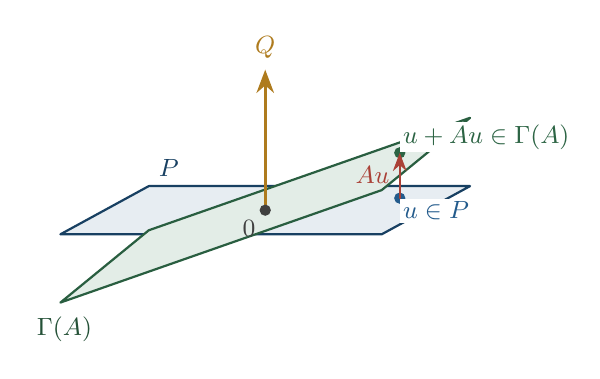
\begin{tikzpicture}[>=Stealth,line cap=round,line join=round,scale=1.02]
 \filldraw[fill=manifoldblue!11,draw=manifoldblue!70!black,thick]
 (-2.55,-.3)--(1.45,-.3)--(2.55,.3)--(-1.45,.3)--cycle;
 \filldraw[fill=manifoldgreen!14,draw=manifoldgreen!75!black,thick]
 (-2.55,-1.15)--(1.45,.25)--(2.55,1.15)--(-1.45,-.25)--cycle;
 \draw[->,manifoldgold!85!black,very thick] (0,0)--(0,1.75)
  node[above,font=\small] {$Q$};
 \fill[black!75] (0,0) circle (2pt) node[below left,font=\small] {$0$};
 \fill[manifoldblue] (1.675,.15) circle (2pt)
  node[below right,fill=white,inner sep=1pt,font=\small] {$u\in P$};
 \fill[manifoldgreen!80!black] (1.675,.715) circle (2pt)
  node[above right,fill=white,inner sep=1pt,font=\small] {$u+Au\in\Gamma(A)$};
 \draw[->,manifoldred,thick] (1.675,.15)--(1.675,.715)
  node[midway,left,font=\small] {$Au$};
 \node[manifoldblue!70!black,font=\small\bfseries] at (-1.2,.52) {$P$};
 \node[manifoldgreen!65!black,font=\small\bfseries] at (-2.5,-1.48) {$\Gamma(A)$};
\end{tikzpicture}
\caption{Mapa wykresowa grassmannianu. Przestrzeń $P$ jest
punktem odniesienia; pobliska płaszczyzna $\Gamma(A)$ powstaje,
gdy nad $u\in P$ odkładamy przemieszczenie $Au\in Q$.}
\label{fig:lin29-grass-wykres}
\end{figure}

\begin{przyklad}[Mała mapa, a nie cały grassmannian]
\label{prz:lin29-grass-rp1-mapy}
Na $\operatorname{Gr}_1(\R^2)=\mathbb{RP}^1$ ustalmy
$P=\R e_1$ i $Q=\R e_2$. Prosta
$L_a=\operatorname{span}(e_1+ae_2)$ ma współrzędną
$a\in\R$. Brakuje dokładnie jednej prostej, $\R e_2$:
rzutowanie na $P$ jest na niej zerowe. Zatem mapa
wykresowa jest lokalna, podobnie jak mapa stereograficzna
nie pokrywa całej sfery.

W drugiej mapie, z $P'=\R e_2$ i $Q'=\R e_1$,
zapisujemy $L=\operatorname{span}(be_1+e_2)$.
Na części wspólnej obu map $a\ne0$ i
\[
 e_1+ae_2=a\bigl(a^{-1}e_1+e_2\bigr),
 \qquad b=\frac1a.
\]
To najprostszy przypadek wzoru~\eqref{eq:lin29-grass-przejscie}:
druga mapa dopisuje prostą $\R e_2$, której nie ma
w pierwszej; jej współrzędna $b=0$ odpowiada
,,$a=\infty$'' w potocznym opisie.
\end{przyklad}

\section{Przestrzeń styczna i wiązka tautologiczna}
\label{sec:lin29-grass-styczna}

Wektor styczny do grassmannianu opisuje \emph{pierwszy
rząd zmiany podprzestrzeni}. Wektory należące już do
danej podprzestrzeni nie zmieniają jej położenia:
istotna jest część wychodząca poza nią.
Z każdej z $k$ niezależnych osi podprzestrzeni możemy
wyjść w $n-k$ niezależnych kierunkach poprzecznych;
stąd intuicyjnie bierze się wymiar $k(n-k)$.

\begin{twierdzenie}[Styczne jako odwzorowania do ilorazu]
\label{thm:lin29-grass-styczna}
Dla $L\in\operatorname{Gr}_k(V)$ istnieje kanoniczny
izomorfizm
\begin{equation}\label{eq:lin29-grass-styczna}
 T_L\operatorname{Gr}_k(V)
  \cong\operatorname{Hom}_{\mathbb K}(L,V/L).
\end{equation}
Nad $\C$ prawa strona jest zespoloną przestrzenią
styczną; jej podłożem rzeczywistym jest rzeczywista
przestrzeń styczna.
\end{twierdzenie}
\begin{proof}
Niech $L(t)$ będzie gładką krzywą podprzestrzeni,
$L(0)=L$. Dla $v\in L$ wybierzmy gładką krzywą
$v(t)\in L(t)$ z $v(0)=v$. Definiujemy
$D_{L'(0)}(v):=[v'(0)]\in V/L$, gdzie nawias oznacza
klasę modulo $L$. Pokażmy niezależność od wyboru
$v(t)$. Różnica dwóch takich krzywych $w(t)\in L(t)$
ma $w(0)=0$. W gładkiej lokalnej bazie $s_i(t)$
zapisuje się $w(t)=\sum_i a_i(t)s_i(t)$ z
$a_i(0)=0$, zatem
$w'(0)=\sum_i a_i'(0)s_i(0)\in L$. Klasa
$[v'(0)]$ nie zmienia się. Zmiana parametryzacji
krzywej nie jest jedyną możliwą zmianą przedstawiciela wektora
stycznego; niezależność od dowolnej krzywej o tym samym wektorze
stycznym sprawdzimy teraz w mapie.

Ustalmy teraz uzupełnienie $V=L\oplus Q$.
W mapie z Twierdzenia~\ref{thm:lin29-grass-atlas} mamy
$L(t)=\Gamma(A(t))$ i $A(0)=0$.
Wybieramy $v(t)=v+A(t)v$. Wtedy
\[
 D_{L'(0)}(v)=[A'(0)v]\in V/L.
\]
Tak samo $s_i(t)=e_i+A(t)e_i$ dla bazy $(e_i)$ przestrzeni $L$
daje gładką bazę używaną powyżej. Wzór zależy tylko od $A'(0)$,
czyli współrzędnych wektora stycznego, a nie od dalszego przebiegu krzywej.
Jeśli $D_{L'(0)}=0$, to $A'(0)v\in Q\cap L=0$ dla każdego $v$,
więc $A'(0)=0$ i wektor styczny jest zerowy. To dowodzi iniektywności.
Utożsamienie $Q\cong V/L$ pokazuje, że
$D_{L'(0)}$ jest liniowe w $v$. Każdy
$D\in\operatorname{Hom}(L,V/L)$ można otrzymać:
wybierzmy odpowiadające mu odwzorowanie $A:L\to Q$
i krzywą $L(t)=\Gamma(tA)$. Jej pochodna daje
właśnie $D$. Konstrukcja rozpoczęła się od
krzywej i klas modulo $L$, więc otrzymany
izomorfizm nie zależy od wybranego $Q$.
\end{proof}

\begin{przyklad}[Wektor styczny do przestrzeni prostych]
Niech $L_0=\R e_1\in\operatorname{Gr}_1(\R^2)$ i
$L(t)=\R(e_1+t e_2)$. W mapie z
Przykładu~\ref{prz:lin29-grass-rp1-mapy}
współrzędna krzywej to $a(t)=t$, więc jej prędkość
wynosi $a'(0)=1$. Dla wektora $v=s e_1\in L_0$
wybieramy $v(t)=s(e_1+t e_2)\in L(t)$; z definicji
\[
 D_{L'(0)}(s e_1)=[s e_2]\in\R^2/L_0.
\]
Zatem pojedyncza liczba $a'(0)$ jest macierzą
odwzorowania $L_0\to\R^2/L_0$ w bazach
$e_1$ i $[e_2]$. Krzywa
$\widetilde L(t)=\R(\cos t\,e_1+\sin t\,e_2)$
daje ten sam wektor styczny, bo jej współrzędna
$\tan t$ także ma pochodną $1$ w zerze.
\end{przyklad}

\begin{definicja}[Wiązka tautologiczna]
\index{wiazka tautologiczna@Wiązka tautologiczna}
\label{def:lin29-grass-taut}
Nad $\operatorname{Gr}_k(V)$ określamy
\emph{wiązkę tautologiczną}
\[
 \gamma^k
 :=\{(L,v)\in\operatorname{Gr}_k(V)\times V:v\in L\}
 \longrightarrow\operatorname{Gr}_k(V),\qquad (L,v)\mapsto L.
\]
Jej włókno w punkcie $L$ jest dosłownie podprzestrzenią
$L\subseteq V$.
\end{definicja}

\begin{stwierdzenie}[Lokalność i wiązka ilorazowa]
\label{prop:lin29-grass-wiazki}
Wiązka $\gamma^k$ ma rząd $k$. Jest podwiązką
wiązki trywialnej $\operatorname{Gr}_k(V)\times V$.
Istnieje też wiązka ilorazowa $\mathcal Q$ z
włóknem $\mathcal Q_L=V/L$, rzędu $n-k$,
oraz kanoniczny dokładny ciąg wiązek
\begin{equation}\label{eq:lin29-grass-ciag}
 0\longrightarrow\gamma^k
 \longrightarrow\operatorname{Gr}_k(V)\times V
 \longrightarrow\mathcal Q\longrightarrow0.
\end{equation}
Po wybraniu iloczynu skalarnego otrzymujemy
$\mathcal Q\cong(\gamma^k)^\perp$.
\end{stwierdzenie}
\begin{proof}
Na $U_P$ każdy element $L=\Gamma(A)$ zawiera
dokładnie jeden wektor $u+Au$ dla danego $u\in P$.
Odwzorowanie $(L,u)\mapsto(L,u+Au)$ jest zatem lokalną
trywializacją $U_P\times P\cong\gamma^k|_{U_P}$;
jej odwrotność to $(L,v)\mapsto(L,\pi_Pv)$.
Oba odwzorowania są gładkie, a na włóknach liniowe.
W tym samym rozkładzie $V=P\oplus Q$ klasa
$[w]\in V/\Gamma(A)$ ma jednoznacznego
reprezentanta w $Q$: od $w$ odejmujemy
$u+Au\in\Gamma(A)$, gdzie $u=\pi_Pw$.
Stąd lokalnie $\mathcal Q|_{U_P}\cong U_P\times Q$.
Na każdym włóknie inkluzja $L\hookrightarrow V$
jest iniekcją, a naturalne odwzorowanie $V\to V/L$ jest
surjekcją z jądrem $L$, co wyjaśnia \emph{dokładność}
ciągu~\eqref{eq:lin29-grass-ciag}. Iloczyn skalarny
identyfikuje klasę $[v]$ z $(\id-\Pi_L)v\in L^\perp$.
Rzut zależy gładko od $L$, więc jest to izomorfizm wiązek,
a nie tylko rodzina izomorfizmów włókien.
\end{proof}

\begin{uwaga}[Styczna i iloczyn tensorowy]
Twierdzenie~\ref{thm:lin29-grass-styczna} i
izomorfizm tensorowy~\ref{thm:lin10-hom-rzad} dają
\[
 T\operatorname{Gr}_k(V)\cong
       (\gamma^k)^*\otimes\mathcal Q.
\]
Włókno po prawej stronie w $L$ to
$L^*\otimes(V/L)\cong\operatorname{Hom}(L,V/L)$.
Kolejność czynników jest tu ważna: źródłem odwzorowania
jest $L$, a jego wartości należą do $V/L$.
Zgodność tych izomorfizmów z gładkością również widać w mapie:
przy $L=\Gamma(A)$ przyrost $\dot A$ wysyła $u+Au$ na
klasę $\dot A u$. W trywializacji ilorazu
$[w]\mapsto\pi_Qw-A\pi_Pw$ ma on po prostu macierz $\dot A$.
Zatem izomorfizmy włókien sklejają się w gładki izomorfizm wiązek.
\end{uwaga}

\begin{przyklad}[Proste w płaszczyźnie i wstęga Möbiusa]
Na $\operatorname{Gr}_1(\R^2)\cong\mathbb{RP}^1\cong S^1$
wiązka $\gamma^1$ jest wstęgą Möbiusa (co wynika z poniższego obliczenia). Istotnie,
$L(t)=\R(\cos t,\sin t)$, $0\leq t\leq\pi$,
opisuje pełne okrążenie bazy: $L(0)=L(\pi)$.
Wybrany lokalnie wektor jednostkowy
$(\cos t,\sin t)\in L(t)$ wraca jako jego
przeciwieństwo. To właśnie sklejanie włókna
ze zmianą znaku.
W dwóch mapach z Przykładu~\ref{prz:lin29-grass-rp1-mapy} tę zmianę
widać również w funkcji przejścia: jeśli
$\lambda(e_1+ae_2)=\mu(be_1+e_2)$ oraz $b=1/a$,
to porównanie współczynników daje $\mu=a\lambda$.
Na dwóch składowych części wspólnej ($a>0$ i $a<0$)
funkcja przejścia ma przeciwne znaki. Właśnie tego
nie da się usunąć przez jeden globalny wybór
niezerowego wektora w każdym włóknie: zmiana
lokalnej ramki (czyli lokalnego nigdzie niezerowego przekroju)
przez funkcję nigdzie niezerową
ma na każdej spójnej mapie stały znak.
\end{przyklad}

\section{Orientacja, współrzędne Plückera i odwzorowanie Gaussa}
\label{sec:lin29-grass-plucker}

\begin{definicja}[Grassmannian zorientowany]
\index{grassmannian zorientowany@Grassmannian zorientowany}
Punkt $\operatorname{Gr}^+_k(\R^n)$ to para $(L,o)$:
$k$-płaszczyzna $L$ wraz z wyborem jej orientacji $o$.
Zapomnienie orientacji daje dwukrotne nakrycie
$\operatorname{Gr}^+_k(\R^n)\to\operatorname{Gr}_k(\R^n)$
dla $0<k<n$: nad każdą płaszczyzną są dokładnie
dwie możliwe orientacje. W mapie wykresowej
orientację przenosimy z $P$ na $\Gamma(A)$ przez
$u\mapsto u+Au$, więc lokalnie nakrycie jest
sumą dwóch kopii tej samej mapy.
\end{definicja}

\begin{przyklad}[Płaszczyzny w $\R^3$]
Płaszczyźnie $L\in\operatorname{Gr}_2(\R^3)$
odpowiada jej nieukierunkowana prosta normalna
$L^\perp$, a zatem
$\operatorname{Gr}_2(\R^3)\cong\mathbb{RP}^2$.
Gdy $L$ ma orientację, wybierzmy dodatnią bazę
ortonormalną $(u,v)$ i połóżmy $n=u\times v$.
Inna dodatnia baza różni się obrotem w $L$,
więc daje ten sam $n$. W drugą stronę $n\in S^2$
wyznacza $L=n^\perp$ i orientację, dla której
$(u,v,n)$ jest dodatnią bazą $\R^3$. Otrzymujemy
\[
 \operatorname{Gr}^+_2(\R^3)\cong S^2,\qquad
 \operatorname{Gr}_2(\R^3)\cong S^2/(n\sim -n).
\]
Zmiana orientacji płaszczyzny zamienia $n$ z $-n$.
Dla ustalenia gładkości zauważmy, że normalna z lokalnej dodatniej
ramki ortonormalnej jest gładka. W drugą stronę rzut
na $n^\perp$ ma macierz $I-nn^T$, gładką w $n$;
lokalny wybór orientacji jest stały na każdym z dwóch płatów.
Są to więc dyfeomorfizmy, nie tylko bijekcje zbiorów.
\end{przyklad}

\begin{figure}[!htbp]
\centering
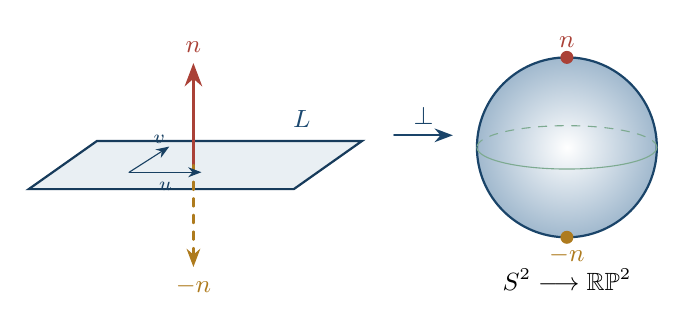
\begin{tikzpicture}[>=Stealth,line cap=round,scale=1.02]
 \filldraw[fill=manifoldblue!10,draw=manifoldblue!65!black,thick]
 (-4.6,-.52)--(-1.3,-.52)--(-.45,.08)--(-3.75,.08)--cycle;
 \draw[->,very thick,manifoldred] (-2.55,-.22)--(-2.55,1.05)
   node[above,font=\small] {$n$};
 \draw[->,thick,manifoldgold!85!black,dashed]
   (-2.55,-.22)--(-2.55,-1.49)
   node[below,font=\small] {$-n$};
 \node[font=\small,manifoldblue!80!black] at (-1.2,.35) {$L$};
 \draw[->,manifoldblue!70!black] (-3.35,-.31)--(-2.45,-.31)
   node[midway,below,font=\scriptsize] {$u$};
 \draw[->,manifoldblue!70!black] (-3.35,-.31)--(-2.85,.01)
   node[near end,above,font=\scriptsize] {$v$};
 \shade[inner color=white,outer color=manifoldblue!43] (2.1,0) circle (1.12);
 \draw[manifoldblue!75!black,thick] (2.1,0) circle (1.12);
 \draw[manifoldgreen!65,thin] (.98,0) arc[start angle=180,end angle=360,x radius=1.12,y radius=.27];
 \draw[manifoldgreen!65,thin,dashed] (3.22,0)
   arc[start angle=0,end angle=180,x radius=1.12,y radius=.27];
 \fill[manifoldred] (2.1,1.12) circle (2.3pt)
   node[above,font=\small] {$n$};
 \fill[manifoldgold!85!black] (2.1,-1.12) circle (2.3pt)
   node[below,font=\small] {$-n$};
 \draw[->,manifoldblue!75!black,thick] (-.05,.15)--(.68,.15)
   node[midway,above,font=\small] {$\perp$};
 \node[font=\small] at (2.1,-1.65) {$S^2\longrightarrow\mathbb{RP}^2$};
\end{tikzpicture}
\caption{Orientacja płaszczyzny w $\R^3$ wybiera jedną z
dwóch jednostkowych normalnych. Zapomnienie orientacji
utożsamia punkty antypodyczne $n$ i $-n$ na sferze.}
\label{fig:lin29-grass-normalne}
\end{figure}

\begin{stwierdzenie}[Bazy ortonormalne i przestrzeń ilorazowa]
\label{prop:lin29-grass-stiefel}
Niech $V_k(\R^n)$ będzie zbiorem uporządkowanych
ortonormalnych $k$-ramek $(v_1,\ldots,v_k)$.
Odwzorowanie $(v_i)\mapsto\operatorname{span}(v_i)$ ma
włókna izomorficzne z $\mathrm O(k)$.
Ponadto, jako gładkie przestrzenie,
\[
 \operatorname{Gr}_k(\R^n)
   \cong\mathrm O(n)/(\mathrm O(k)\times\mathrm O(n-k)),
\quad
 \operatorname{Gr}_k(\C^n)
   \cong\mathrm U(n)/(\mathrm U(k)\times\mathrm U(n-k)).
\]
\end{stwierdzenie}
\begin{proof}
Dwie ramki wyznaczają tę samą $k$-płaszczyznę wtedy
i tylko wtedy, gdy zmiana bazy między nimi należy do
$\mathrm O(k)$. Wykonując ortonormalizację Grama--Schmidta
na wektorach $u_i+Au_i$ z mapy wykresowej, dostajemy
gładki lokalny wybór ramki; włókna są więc lokalnie
kopiami $\mathrm O(k)$. Grupa $\mathrm O(n)$ działa
tranzytywnie na płaszczyznach: wybieramy bazy ortonormalne
dwóch płaszczyzn, uzupełniamy je do baz $\R^n$ i bierzemy
odwzorowanie przenoszące pierwszą pełną bazę na drugą.
Element zachowujący standardowe $\R^k$ zachowuje też
jego dopełnienie prostopadłe, czyli ma postać blokową
$\mathrm{diag}(B,C)$ z $B\in\mathrm O(k)$,
$C\in\mathrm O(n-k)$. To daje pierwszy iloraz.
Wyjaśnijmy gładką strukturę ilorazu. W rozkładzie ortogonalnym
$P\oplus Q$ uzupełniamy ramkę wykresu przez ramkę
$\Gamma(-A^*)\subset Q\oplus P$ jego dopełnienia prostopadłego:
jej wektory mają postać $-A^*w+w$, $w\in Q$.
Ortonormalizacja obu ramek daje macierz $s(A)\in\mathrm O(n)$
zależną gładko od $A$. Każda macierz ortogonalna nad tą mapą
ma jednoznaczną postać $s(A)\operatorname{diag}(B,C)$.
Parametr $A$ odzyskujemy z obrazu pierwszych $k$ kolumn,
a bloki $B,C$ z iloczynu $s(A)^{-1}O$. Daje to lokalny
produkt i jego gładką odwrotność; po podzieleniu przez bloki
pozostaje dokładnie mapa wykresowa grassmannianu.
Argument dla $\C$ jest taki sam, z bazami unitarnymi,
sprzężeniem hermitowskim i grupą $\mathrm U(n)$.
\end{proof}

Iloczyn zewnętrzny z Sekcji~\ref{sec:lin11-zewnetrzna}
pozwala zapisać $k$-płaszczyznę jednym wielowektorem,
określonym z dokładnością do niezerowego skalara.
Po wyborze bazy $(e_i)$ przestrzeni $V$ oraz zapisaniu
$v_j=\sum_i v_{ij}e_i$ współczynnik
$p_I$ przy $e_{i_1}\wedge\cdots\wedge e_{i_k}$
ma postać minora
$\det(v_{i_a j})_{1\leq a,j\leq k}$, gdzie
$I=(i_1<\cdots<i_k)$; jest to
wzór z Wniosku~\ref{cor:lin11-wedge-minory}.
Liczby $p_I$ nazywamy \emph{współrzędnymi Plückera}.
Zmiana bazy $L$ mnoży je wszystkie przez tę samą
niezerową liczbę $\det C$, więc geometryczną informację
niesie ich klasa rzutowa $[p_I]$.

\begin{twierdzenie}[Zanurzenie Plückera]
\label{thm:lin29-grass-plucker}
Jeśli $(v_1,\ldots,v_k)$ jest bazą $L$, to wzór
\begin{equation}\label{eq:lin29-plucker}
 \mathrm{Pl}(L):=[v_1\wedge\cdots\wedge v_k]
 \in\mathbb P(\Lambda^k V)
\end{equation}
określa gładkie zanurzenie
$\operatorname{Gr}_k(V)\hookrightarrow\mathbb P(\Lambda^k V)$.
Nawias $[\xi]$ oznacza prostą $\mathbb K\xi$,
$\xi\ne0$. Obraz składa się dokładnie z klas
niezerowych \emph{wielowektorów prostych}.
\end{twierdzenie}
\begin{proof}
Zmiana bazy $(v_i)$ macierzą $C$ mnoży iloczyn
zewnętrzny przez $\det C\ne0$ na mocy
Twierdzenia~\ref{thm:lin11-det-wedge}, więc klasa
rzutowa jest dobrze określona. Jeżeli
$\xi=v_1\wedge\cdots\wedge v_k\ne0$, to
\[
 L=\{w\in V:w\wedge\xi=0\}.
\]
Wektory z $L$ dają zero przez powtórzenie czynnika.
Jeśli $w\notin L$, rodzina $(v_1,\ldots,v_k,w)$
jest liniowo niezależna; po uzupełnieniu do bazy
Twierdzenie~\ref{thm:lin11-zew-baza} mówi, że jej
iloczyn zewnętrzny jest niezerowy. Zatem
$\mathrm{Pl}(L)$ wyznacza $L$ jednoznacznie.

Pokażmy, skąd bierze się gładki odwrotny wzór na obrazie.
W mapie $V=P\oplus Q$ wybierzmy bazy
$e_1,\ldots,e_k$ przestrzeni $P$ oraz
$e_{k+1},\ldots,e_n$ przestrzeni $Q$ i zapiszmy
$Ae_j=\sum_{a=1}^{n-k}a_{aj}e_{k+a}$.
W wielowektorze
$\xi_A=(e_1+Ae_1)\wedge\cdots\wedge(e_k+Ae_k)$
współczynnik $p_{1\cdots k}$ wynosi $1$.
Współczynnik przy
$e_1\wedge\cdots\wedge\widehat{e_j}\wedge\cdots
\wedge e_k\wedge e_{k+a}$ wynosi
$(-1)^{k-j}a_{aj}$: przesuwamy $e_{k+a}$
przez $k-j$ późniejszych czynników.
Z ilorazów tych współczynników przez $p_{1\cdots k}$
odzyskujemy wszystkie $a_{aj}$.
Jeśli dla dowolnego indeksu $I$ mamy $p_I\ne0$,
to rzut bazy $L$ na płaszczyznę
$P=\operatorname{span}\{e_i:i\in I\}$ ma wyznacznik $p_I$.
Jest więc izomorfizmem $L\to P$ i możemy stosować
analogiczny wzór w mapie $U_P$, dzieląc przez $p_I$.
Odwzorowanie~\eqref{eq:lin29-plucker} jest więc gładkie.
Wzory odzyskujące $a_{aj}$ są określone na całym otwartym
zbiorze przestrzeni rzutowej $p_{1\cdots k}\ne0$, nie tylko
na obrazie. Ich złożenie z $\mathrm{Pl}$ jest odwzorowaniem identycznościowym
w parametrach $A$; różniczkowanie daje lewą odwrotność różniczki
$\mathrm{Pl}$, która jest zatem injektywna.
Otrzymaliśmy immersję. Grupy $\mathrm O(n)$ i $\mathrm U(n)$
są zwarte jako domknięte i ograniczone zbiory macierzy.
Ich ilorazy z~\ref{prop:lin29-grass-stiefel}, a więc oba
grassmanniany, są zwarte jako ciągłe obrazy grup zwartych.
Ponieważ przestrzeń rzutowa jest Hausdorffa,
ciągła iniekcja ze zwartego grassmannianu jest
homeomorfizmem na obraz. To daje zanurzenie i domkniętość obrazu.
\end{proof}

\begin{przyklad}[Relacja Plückera dla $\operatorname{Gr}_2(\R^4)$]
Zapiszmy $\xi=\sum_{1\leq i<j\leq4}p_{ij}e_i\wedge e_j$.
Rozwińmy $\xi\wedge\xi$. Składnik z powtórzonym
indeksem znika, więc zostają tylko pary $12|34$, $13|24$
i $14|23$ oraz te same pary w odwrotnej kolejności.
Pierwsza para jest już uporządkowana; w drugiej
przestawienie $1,3,2,4$ do $1,2,3,4$ wymaga jednej
transpozycji, a w trzeciej przestawienie $1,4,2,3$
wymaga dwóch. Znaki wynoszą zatem kolejno $+,-,+$.
Każda para występuje dwukrotnie z tym samym znakiem,
bo zamiana dwóch bloków stopnia $2$ daje $(-1)^4=1$.
Otrzymujemy
\begin{equation}\label{eq:lin29-plucker-24}
 \xi\wedge\xi=
 2(p_{12}p_{34}-p_{13}p_{24}+p_{14}p_{23})
   e_1\wedge e_2\wedge e_3\wedge e_4.
\end{equation}
Jeżeli $\xi=u\wedge v$, to $\xi\wedge\xi=0$,
więc współczynniki spełniają relację w nawiasie.
Odwrotnie, dla $\xi\ne0$ z taką relacją możemy
przestawić współrzędne tak, by $p_{12}\ne0$.
Po podzieleniu przez $p_{12}$ ustawiamy w wykresie
$e_1+ae_3+ce_4$, $e_2+be_3+de_4$ liczby
$b=p_{13}/p_{12}$, $d=p_{14}/p_{12}$,
$a=-p_{23}/p_{12}$, $c=-p_{24}/p_{12}$.
Pięć współczynników się zgadza z definicji,
a szósty jest równy $ad-bc=p_{34}/p_{12}$
właśnie dzięki relacji: po podstawieniu
$ad-bc=(p_{13}p_{24}-p_{14}p_{23})/p_{12}^2$,
a relacja daje w liczniku $p_{12}p_{34}$.
To dowodzi również
wystarczalności.

Policzmy wszystkie współrzędne dla
$L=\operatorname{span}(e_1+2e_3,e_2+e_4)$:
\[
 (e_1+2e_3)\wedge(e_2+e_4)
  =e_1\wedge e_2+e_1\wedge e_4
   -2e_2\wedge e_3+2e_3\wedge e_4.
\]
Mamy więc $(p_{12},p_{13},p_{14},p_{23},p_{24},p_{34})
=(1,0,1,-2,0,2)$ i relację $1\cdot2+1\cdot(-2)=0$.
Z kolei współrzędne wykresu odzyskujemy jako
$(a,b,c,d)=(2,0,0,1)$, zgodnie z wyjściową bazą.
W tym przypadku $\dim\operatorname{Gr}_2(\R^4)=4$,
podczas gdy $\mathbb P(\Lambda^2\R^4)$ ma wymiar $5$:
jedna relacja $p_{12}p_{34}-p_{13}p_{24}+p_{14}p_{23}=0$
opisuje więc cały obraz Plückera jako kwadrykę rzutową.
Dla kontrastu
$e_1\wedge e_2+e_3\wedge e_4$ ma
$p_{12}p_{34}=1$ i pozostałe wyrazy zerowe,
więc nie jest wielowektorem prostym, zgodnie
z wcześniejszym Przykładem w
Sekcji~\ref{sec:lin11-baza-wedge}.
\end{przyklad}

\begin{twierdzenie}[Odwzorowanie Gaussa i wiązka styczna]
\label{thm:lin29-grass-gauss}
Niech $M^m\subset\R^N$ będzie gładką podrozmaitością.
Przypisanie
$G(p)=T_pM\in\operatorname{Gr}_m(\R^N)$
jest gładkim \emph{odwzorowaniem Gaussa}. Wiązki
$TM$ i normalna $\nu M$ są odpowiednio
cofnięciami $G^*\gamma^m$ i $G^*\mathcal Q$
z~\eqref{eq:lin29-grass-ciag}.
\end{twierdzenie}
\begin{proof}
W mapie podrozmaitości zapisujemy jej parametryzację
$F:U\subset\R^m\to\R^N$. Wektory
$\partial_iF(x)$ tworzą gładką bazę $T_{F(x)}M$.
W pobliżu ustalonego punktu pewien minor $m\times m$
macierzy $DF$ pozostaje niezerowy. W odpowiadającym
mu rozkładzie $\R^N=P\oplus Q$ przestrzeń
$T_{F(x)}M$ jest wykresem macierzy
$A(x)=D_QF(x)(D_PF(x))^{-1}$,
gładkiej w $x$. Stąd $G$ jest gładka.
Włókno $(G^*\gamma^m)_p$ to z definicji
$\gamma^m_{G(p)}=T_pM$; lokalne ramki po obu
stronach są tymi samymi $\partial_iF$.
Włókno $(G^*\mathcal Q)_p$ to
$\R^N/T_pM$, czyli $\nu_pM$ (po utożsamieniu przez iloczyn skalarny) z przestrzenią normalną $(T_pM)^\perp$.
Zgodność lokalnych trywializacji daje oba
izomorfizmy wiązek.
\end{proof}

\begin{przyklad}[Odwzorowanie Gaussa paraboli]
Dla paraboli $M=\{(t,t^2):t\in\R\}\subset\R^2$
weźmy parametryzację $F(t)=(t,t^2)$. Wówczas
\[
 F'(t)=(1,2t),\qquad
 G(F(t))=\R(1,2t),\qquad a(t)=2t
\]
w mapie $\operatorname{Gr}_1(\R^2)$ z
Przykładu~\ref{prz:lin29-grass-rp1-mapy}.
W punkcie $p=F(0)$ różniczka odwzorowania Gaussa
odpowiada, według~\eqref{eq:lin29-grass-styczna},
odwzorowaniu $T_pM\to\R^2/T_pM$ danemu przez
$e_1\mapsto2[e_2]$. Liczba $2$ mierzy tutaj
pierwszy rząd zmiany kierunku stycznej, podczas gdy
położenie punktu $F(t)$ nie występuje we współrzędnej $a(t)$.
Po utożsamieniu ilorazu z prostopadłą prostą
jednostkowa normalna ma postać
$(-2t,1)/\sqrt{1+4t^2}$.
\end{przyklad}

\begin{uwaga}[Dlaczego wiązka tautologiczna jest uniwersalna?]
Na zwartej rozmaitości każdą gładką rzeczywistą wiązkę $E$
rzędu $k$ można umieścić w trywialnej wiązce
$M\times\R^N$ dla pewnego $N$.
Oto konstrukcja. Wybieramy skończone pokrycie
trywializujące $U_i$, jego mniejsze podpokrycie
oraz funkcje gładkie $\beta_i$ o nośnikach w $U_i$,
takie że dla każdego $p$ co najmniej jedna
$\beta_i(p)$ jest niezerowa. Jeśli $[v]_i\in\R^k$
oznacza współrzędne $v\in E_p$ na $U_i$,
definiujemy różnowartościowe odwzorowanie liniowe w $v$
\[
 j_p(v)=\bigl(\beta_1(p)[v]_1,\ldots,
                  \beta_r(p)[v]_r\bigr)\in\R^{kr},
\]
przyjmując wartość $0$ dla bloku poza $U_i$.
Podparcie $\beta_i$ wewnątrz $U_i$ zapewnia
gładkość po przedłużeniu zerem; co najmniej
jeden niezerowy blok zapewnia iniektywność $j_p$.
Obrazy $j_p(E_p)$ zmieniają się gładko, ponieważ
lokalnie tworzą kolumny macierzy gładkiej i
stałego rzędu $k$, a więc definiują odwzorowanie
$f:M\to\operatorname{Gr}_k(\R^{kr})$.
Wprost z definicji włókien mamy
$E\cong f^*\gamma^k$. Ta konkretna konstrukcja
wyjaśnia użyteczność grassmannianów dla topologii
wiązek; nie potrzebuje jeszcze teorii klas
charakterystycznych.
W przypadku wiązki zespolonej ten sam rachunek
prowadzimy w $\C^{kr}$ i otrzymujemy mapę do
$\operatorname{Gr}_k(\C^{kr})$.
\end{uwaga}


\chapter{Algebry Clifforda}
\label{ch:lin30-clifford}
\index{algebry Clifforda}

W algebrze zewnętrznej z Rozdziału~\ref{ch:lin11-algebry}
iloczyn wektora przez siebie jest równy zeru.
Iloczyn Clifforda uwzględnia również formę kwadratową.
Zbudujemy go jako iloraz algebry tensorowej, uzasadnimy jego
własność uniwersalną oraz dowiedziemy wzoru na wymiar
bez zakładania niezależności normalnych monomów.

\section{Algebra Clifforda: iloczyn i dowód wymiaru}
\label{sec:lin30-clifford}

Od tego miejsca $V$ jest rzeczywistą przestrzenią
euklidesową wymiaru $n$ z iloczynem skalarnym
$\langle\cdot,\cdot\rangle$ i normą
$\|v\|^2=\langle v,v\rangle$. Algebra zewnętrzna
pamięta zorientowane pola: $v\wedge v=0$.
Algebra Clifforda pamięta ponadto \emph{długość}:
kwadrat wektora jest skalarem $-\|v\|^2$.
Przyjmujemy konsekwentnie ten znak minus;
w literaturze spotyka się również konwencję przeciwną.

\begin{definicja}[Algebra Clifforda]
\index{algebra clifforda@Algebra Clifforda}
\label{def:lin30-clifford}
Niech $I_q$ będzie ideałem obustronnym algebry
tensorowej $T(V)$ z Definicji~\ref{def:lin11-tensorowa},
generowanym przez
$v\otimes v+\|v\|^2\,1$ dla wszystkich $v\in V$.
\emph{Algebra Clifforda} to
\[
 \operatorname{Cl}(V):=T(V)/I_q.
\]
Obraz $v\in V$ oznaczamy nadal $v$,
a mnożenie w ilorazie zapisujemy bez symbolu $\otimes$.
Z definicji $v^2=-\|v\|^2\,1$.
\end{definicja}

Po usunięciu z relacji składnika $\|v\|^2\,1$
otrzymujemy algebrę zewnętrzną
(Definicja~\ref{def:lin11-zewnetrzna}).
Tak więc obie algebry startują z tej samej algebry
tensorowej; zmieniamy tylko relację, przez którą
dzielimy. W algebrze Clifforda nie można zachować
zwykłego stopnia tensorowego: relacja utożsamia
wyraz stopnia $2$ ze skalarem stopnia $0$.
Pozostaje rozróżnienie stopnia \emph{parzystego}
i \emph{nieparzystego}, bo oba wyrazy relacji
mają tę samą parzystość.
Oznaczamy odpowiadające podprzestrzenie przez
$\operatorname{Cl}^0(V)$ i $\operatorname{Cl}^1(V)$.
Jest to suma prosta: ideał $I_q$ rozkłada się na części
parzystą i nieparzystą, ponieważ jego generatory są parzyste,
a każdy mnożnik po lewej i prawej można rozdzielić
według parzystości. Iloraz zachowuje więc ten rozkład.
Iloczyn słów o parzystościach $i,j\in\{0,1\}$
ma parzystość $i+j$ modulo $2$; jest to
$\Z/2\Z$-stopniowanie algebry Clifforda.

\begin{twierdzenie}[Relacja Clifforda i własność uniwersalna]
\label{thm:lin30-cliff-relacje}
Dla $v,w\in V$ w $\operatorname{Cl}(V)$ zachodzi
\begin{equation}\label{eq:lin30-cliff-relacja}
 vw+wv=-2\langle v,w\rangle\,1.
\end{equation}
Jeżeli $\mathcal A$ jest łączną algebrą rzeczywistą
z jedynką, a $f:V\to\mathcal A$ jest liniowa i spełnia
$f(v)^2=-\|v\|^2 1_{\mathcal A}$ dla każdego $v$,
to istnieje dokładnie jeden homomorfizm algebr
$\widehat f:\operatorname{Cl}(V)\to\mathcal A$
przedłużający $f$.
\end{twierdzenie}
\begin{proof}
Rozwijając $(v+w)^2$ na dwa sposoby, otrzymujemy
\[
 v^2+vw+wv+w^2=-\|v+w\|^2\,1
  =-(\|v\|^2+\|w\|^2+2\langle v,w\rangle)\,1.
\]
Po odjęciu $v^2=-\|v\|^2 1$ i
$w^2=-\|w\|^2 1$ zostaje~\eqref{eq:lin30-cliff-relacja}.
Z Twierdzenia~\ref{thm:lin11-tensorowa-uniwersalna}
odwzorowanie $f$ przedłuża się jednoznacznie do homomorfizmu
$F:T(V)\to\mathcal A$. Dla każdego generatora ideału
$I_q$ mamy
$F(v\otimes v+\|v\|^2 1)
 =f(v)^2+\|v\|^2 1_{\mathcal A}=0$.
Jądro homomorfizmu jest ideałem, więc zawiera $I_q$.
Wobec tego wzór $\widehat f([t])=F(t)$
nie zależy od przedstawiciela $t\in T(V)$
i wyznacza żądany homomorfizm na ilorazie.
Jednoznaczność wynika stąd, że $V$ i jedynka
generują $\operatorname{Cl}(V)$.
\end{proof}

Przy bazie ortonormalnej $(e_1,\ldots,e_n)$
relacja~\eqref{eq:lin30-cliff-relacja} mówi
\begin{equation}\label{eq:lin30-cliff-orto}
 e_i^2=-1,\qquad e_ie_j=-e_je_i\quad(i\ne j).
\end{equation}
Stąd każdy iloczyn generatorów można uporządkować
rosnąco, redukując powtórzone indeksy.
Trudniejszą częścią jest wykazanie, że tak otrzymane
wyrazy nie mają dodatkowych relacji.

\begin{twierdzenie}[Baza algebry Clifforda]
\label{thm:lin30-cliff-baza}
Dla bazy ortonormalnej $e_1,\ldots,e_n$ elementy
\[
 1,\qquad e_{i_1}\cdots e_{i_r}
 \quad(1\leq i_1<\cdots<i_r\leq n,\ 1\leq r\leq n)
\]
stanowią bazę $\operatorname{Cl}(V)$. Zatem
$\dim_\R\operatorname{Cl}(V)=2^n$.
Dla $n\geq1$ części parzysta i nieparzysta mają
po $2^{n-1}$ wymiarów.
\end{twierdzenie}
\begin{proof}
\emph{Rozpinanie.} Obrazy słów $v_1\cdots v_r$
rozpinają iloraz $T(V)/I_q$. Po rozwinięciu każdego
$v_j$ w bazie wystarczą słowa z liter $e_i$.
Równości~\eqref{eq:lin30-cliff-orto} pozwalają zamienić
każde dwie sąsiednie różne litery (ze zmianą znaku)
i usunąć parę równych liter ($e_i^2=-1$).
Powtarzając te operacje, dostajemy kombinację
iloczynów o rosnących, różnych indeksach.

\emph{Niezależność.} Skorzystamy z algebry zewnętrznej
$\Lambda(V)$ z Rozdziału~\ref{ch:lin11-algebry}.
Na niej określmy dwie operacje:
\[
 \varepsilon(v)\omega:=v\wedge\omega,\qquad
 \iota_v(w_1\wedge\cdots\wedge w_r)
 :=\sum_{j=1}^r(-1)^{j-1}
   \langle v,w_j\rangle\,
   w_1\wedge\cdots\wedge\widehat{w_j}
       \wedge\cdots\wedge w_r .
\]
Kreska nad $w_j$ oznacza pominięcie tego czynnika;
przyjmujemy $\iota_v(1)=0$.
Wzór na $\iota_v$ jest wieloliniowy i alternujący
w $w_j$: przy zamianie dwóch sąsiednich argumentów składniki
pomijające inny argument zmieniają znak przez antysymetrię iloczynu
zewnętrznego, a dwa pozostałe zamieniają się miejscami z przeciwnymi
znakami. Zatem własność uniwersalna
z Twierdzenia~\ref{thm:lin11-potega-wedge-uniwersalna}
zapewnia, że operator jest dobrze określony.
Bezpośrednio z tego wzoru otrzymujemy
\[
 \iota_v(w\wedge\omega)
  =\langle v,w\rangle\omega-w\wedge\iota_v\omega.
\]
Pierwszy składnik powstaje przy usunięciu pierwszego
czynnika; pozostałe mają o jeden minus więcej niż
w $\iota_v\omega$. Usunięcie dwóch czynników
w dwóch przeciwnych kolejnościach daje składniki
o przeciwnych znakach: dla pozycji $p<q$ ich znaki to
$(-1)^{p-1}(-1)^{q-2}$ oraz
$(-1)^{q-1}(-1)^{p-1}$. Po ich dodaniu
otrzymujemy zero, zatem $\iota_v^2=0$.
Również $\varepsilon(v)^2=0$, bo $v\wedge v=0$.
Jeżeli $c(v):=\varepsilon(v)-\iota_v$, to
\[
 c(v)^2
 =-\bigl(\varepsilon(v)\iota_v
          +\iota_v\varepsilon(v)\bigr)
 =-\|v\|^2\id_{\Lambda(V)}.
\]
Własność uniwersalna z poprzedniego twierdzenia
daje więc reprezentację
$c:\operatorname{Cl}(V)\to\operatorname{End}_\R(\Lambda V)$.
Przyłóżmy ją do $1\in\Lambda^0V$.
Dla różnych ortonormalnych $e_{i_j}$ wszystkie
kontrakcje pojawiające się podczas kolejnego
działania znikają: nowy $e_{i_j}$ jest prostopadły
do wcześniej utworzonych czynników. Stąd
\[
 c(e_{i_1}\cdots e_{i_r})\,1
    =e_{i_1}\wedge\cdots\wedge e_{i_r},\qquad
 c(1)\,1=1.
\]
Prawa strona przebiega bazę $\Lambda(V)$ z
Twierdzenia~\ref{thm:lin11-zew-baza}. Jeśli kombinacja
uporządkowanych słów znikałaby w algebrze Clifforda,
jej działanie na $1$ dawałoby zerową kombinację
\emph{różnych} wektorów tej bazy. Wszystkie
współczynniki muszą więc być zerowe.
Słów o $r$ indeksach jest $\binom nr$;
sumując po $r$ otrzymujemy $2^n$.
Wreszcie bijekcja $I\mapsto I\triangle\{1\}$
zamienia podzbiory parzystej i nieparzystej
liczności, co dowodzi równości ich liczby.
\end{proof}

Na przykład w $\operatorname{Cl}(\R^2)$ redukcja słowa
$e_2e_1e_2=-e_1e_2^2=e_1$ łączy zamianę sąsiednich
generatorów z relacją $e_2^2=-1$. Dzięki dowodowi
niezależności wiemy, że taka redukcja nie ukrywa
żadnych dodatkowych relacji między słowami uporządkowanymi.

\begin{uwaga}[Podobne przestrzenie, różne mnożenia]
\label{rem:lin30-cliff-zewnetrzna}
Istnieje kanoniczny izomorfizm \emph{przestrzeni liniowych}
$\Lambda V\cong\operatorname{Cl}(V)$: wysyła
$v_1\wedge\cdots\wedge v_r$ na antysymetryzację
$\frac1{r!}\sum_{\sigma\in S_r}\operatorname{sgn}(\sigma)
 v_{\sigma(1)}\cdots v_{\sigma(r)}$.
Jest dobrze określony, bo wyrażenie jest alternujące;
na bazowych wektorach ortonormalnych daje
$e_{i_1}\cdots e_{i_r}$, więc poprzednie twierdzenie
zapewnia odwracalność. Nie jest to jednak izomorfizm
algebr: w $\Lambda V$ mamy $v\wedge v=0$,
a w $\operatorname{Cl}(V)$ mamy
$v^2=-\|v\|^2$. To wyjaśnia, dlaczego obie
przestrzenie mają wymiar $2^n$, choć kodują
inne mnożenia.
\end{uwaga}

\begin{przyklad}[Wymiary $0$, $1$ i $2$]
Dla $V=0$ otrzymujemy $\operatorname{Cl}(0)=\R$.
W wymiarze $1$, przy $e_1^2=-1$, każdy element
ma postać $a+be_1$ i mnoży się jak liczba
$a+bi\in\C$. Stąd $\operatorname{Cl}(\R)\cong\C$
\emph{jako algebra rzeczywista}.
W wymiarze $2$ baza $(1,e_1,e_2,e_1e_2)$
spełnia dokładnie relacje kwaternionów:
$e_1\leftrightarrow i$, $e_2\leftrightarrow j$,
$e_1e_2\leftrightarrow k$, zatem
$\operatorname{Cl}(\R^2)\cong\mathbb H$.
Sprawdźmy brakujący kwadrat i znaki:
$(e_1e_2)^2=-e_1^2e_2^2=-1$,
$e_2e_1=-e_1e_2$,
$e_2(e_1e_2)=-e_1e_2^2=e_1$ oraz
$(e_1e_2)e_1=-e_1^2e_2=e_2$.
Relacje $i^2=j^2=-1$ i $ij=-ji$ dają homomorfizm
wysyłający $e_1,e_2$ na $i,j$.
Obrazy czterech wektorów bazy to $1,i,j,k$, czyli baza
$\mathbb H$, więc ten homomorfizm jest izomorfizmem.
Na przykład $(e_1+2e_2)^2=-5$, podczas gdy
$(e_1+2e_2)\wedge(e_1+2e_2)=0$
w algebrze zewnętrznej. Porównujemy więc kwadraty tego samego wektora.
\end{przyklad}

\begin{stwierdzenie}[Iloczyn wektorów: skalar i dwuwektor]
\label{prop:lin30-cliff-wedge}
Przez powyższy izomorfizm przestrzeni liniowych
iloczyn Clifforda dwóch wektorów rozkłada się na
\begin{equation}\label{eq:lin30-cliff-rozdzial}
 vw=-\langle v,w\rangle
       +\tfrac12(vw-wv)
 \quad\longleftrightarrow\quad
 -\langle v,w\rangle+v\wedge w.
\end{equation}
\end{stwierdzenie}
\begin{proof}
Suma $vw+wv$ jest równa
$-2\langle v,w\rangle$ z~\eqref{eq:lin30-cliff-relacja}.
Dodając połowę tej sumy do połowy różnicy,
odzyskujemy $vw$. Antysymetryzacja
$v\wedge w\mapsto\tfrac12(vw-wv)$
jest przypadkiem stopnia $2$ opisanym w
poprzedniej uwadze.
\end{proof}

Przykładowo, dla $v=e_1+2e_2$ oraz $w=2e_1+e_2$
mamy $\langle v,w\rangle=4$ i
$v\wedge w=(1\cdot1-2\cdot2)e_1\wedge e_2
=-3e_1\wedge e_2$. W algebrze Clifforda dostajemy
więc $vw=-4-3e_1e_2$; część skalarna mierzy
iloczyn skalarny, a część stopnia $2$ mierzy
zorientowane pole równoległoboku.

\begin{figure}[!htbp]
\centering
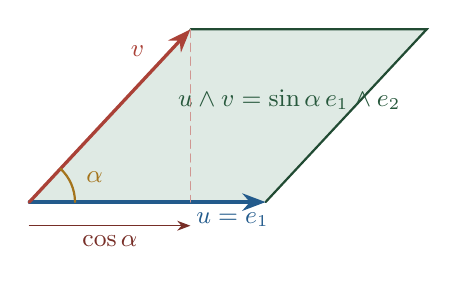
\begin{tikzpicture}[>=Stealth,line cap=round,scale=1.0]
 \coordinate (O) at (0,0);
 \coordinate (U) at (3.0,0);
 \coordinate (W) at ({3*cos(47)},{3*sin(47)});
 \coordinate (UW) at ({3+3*cos(47)},{3*sin(47)});
 \fill[manifoldgreen!16] (O)--(U)--(UW)--(W)--cycle;
 \draw[manifoldgreen!60!black,thick] (U)--(UW)--(W);
 \draw[->,manifoldblue,very thick] (O)--(U)
  node[pos=.86,below,font=\small] {$u=e_1$};
 \draw[->,manifoldred,very thick] (O)--(W)
  node[pos=.78,above left,font=\small] {$v$};
 \draw[densely dashed,manifoldred!55] (W)--({3*cos(47)},0);
 \draw[->,manifoldred!70!black] (0,-.3)--({3*cos(47)},-.3)
  node[midway,below,font=\small] {$\cos\alpha$};
 \draw[manifoldgold!80!black,thick] (.58,0)
  arc[start angle=0,end angle=47,radius=.58];
 \node[manifoldgold!80!black,font=\small] at (.83,.32) {$\alpha$};
 \node[manifoldgreen!70!black,font=\small] at (3.3,1.3)
  {$u\wedge v=\sin\alpha\,e_1\wedge e_2$};
\end{tikzpicture}
\caption{Dla jednostkowych $u=e_1$ i
$v=\cos\alpha\,e_1+\sin\alpha\,e_2$ iloczyn Clifforda
$uv=-\cos\alpha+\sin\alpha\,e_1e_2$ łączy
ujemny iloczyn skalarny ze zorientowanym polem.}
\label{fig:lin30-cliff-iloczyn}
\end{figure}


\chapter{Grupy Pin i Spin, spinory oraz struktury spinowe}
\label{ch:lin31-spinory}

Algebrę Clifforda i jej reprezentację na algebrze zewnętrznej
zbudowaliśmy w Rozdziale~\ref{ch:lin30-clifford}.
W tym rozdziale przejdziemy od iloczynów wektorów jednostkowych
do grup Pin i Spin, a następnie do ich reprezentacji spinowych.
Ostatnia część dotyczy wiązek spinorowych nad rozmaitościami;
używamy w niej pojęć grassmannianu i wiązki wektorowej
wprowadzonych w Rozdziale~\ref{ch:lin29-grassmanniany}.

\section{Od odbić do grupy Spin}
\label{sec:lin31-spin-grupa}

Ustalmy najpierw dwie operacje na algebrze Clifforda.
Zmiana każdego $v$ na $-v$ zachowuje relacje definiujące,
więc daje automorfizm $\alpha$, z $\alpha^2=\id$.
Jego przestrzenie własne dla $+1$ i $-1$ są rozpięte
odpowiednio przez słowa parzyste i nieparzyste; dowód bazy
pokazuje, że ich suma jest prosta.
Drugą operacją jest \emph{rewersja}, oznaczana tyldą:
\[
 \widetilde{v_1\cdots v_r}=v_r\cdots v_1,\qquad
 \widetilde 1=1,
\]
przedłużona liniowo. Jest dobrze określona na ilorazie:
odwracanie słów w $T(V)$ ustala każdy generator
$v\otimes v+\|v\|^2 1$, a element $a(v\otimes v+\|v\|^2 1)b$
wysyła na $\widetilde b(v\otimes v+\|v\|^2 1)\widetilde a$,
nadal należący do ideału. Zatem
$\widetilde{st}=\widetilde t\,\widetilde s$ i
$\widetilde{\widetilde s}=s$, niezależnie od zapisu $s$ jako sumy słów.

Odbicie względem hiperpłaszczyzny prostopadłej
do jednostkowego $u\in V$ ma wzór
\begin{equation}\label{eq:lin31-spin-odbicie}
 r_u(v)=v-2\langle u,v\rangle u.
\end{equation}
Rozkład $v=\langle u,v\rangle u+w$, $w\perp u$,
pokazuje, że $r_u$ odwraca składową równoległą do $u$
i zostawia składową $w$. Jego wyznacznik jest równy $-1$.
Relacja Clifforda daje zaskakujący opis tego odbicia:
ponieważ $u^2=-1$, mamy $u^{-1}=-u$ i
\[
 -uvu^{-1}=uvu
 =-vu^2-2\langle u,v\rangle u
 =v-2\langle u,v\rangle u
 =r_u(v).
\]
W środkowej równości użyliśmy
$uv=-vu-2\langle u,v\rangle$. Znak minus przed
sprzężeniem jest niezbędny, aby obrazem było odbicie
w hiperpłaszczyźnie $u^\perp$ w każdym wymiarze.
Na przykład w $\R^3$ dla $u=e_1$ zwykłe sprzężenie
$v\mapsto uvu^{-1}$ ma w bazie standardowej macierz
$\operatorname{diag}(1,-1,-1)$, natomiast skręcone sprzężenie
$v\mapsto-uvu^{-1}$ ma macierz $\operatorname{diag}(-1,1,1)$.

\begin{definicja}[Grupa Pin]
\label{def:lin31-pin-grupa}
\index{grupa pin@Grupa Pin}
Dla euklidesowej przestrzeni $V$ grupą $\operatorname{Pin}(V)$
nazywamy podgrupę odwracalnych elementów $\operatorname{Cl}(V)$
złożoną ze wszystkich skończonych iloczynów wektorów
jednostkowych; dopuszczamy pusty iloczyn $1$.
W odróżnieniu od grupy Spin dopuszczamy także nieparzystą
liczbę czynników. Dla $s\in\operatorname{Pin}(V)$ określamy
\[
 \rho_{\mathrm{Pin}}(s)(v):=\alpha(s)v s^{-1},
 \qquad v\in V,
\]
gdzie $\alpha$ zmienia znak każdego wektora, jak wyżej.
\end{definicja}

Wzór jest skręconym sprzężeniem: dla jednostkowego $u$
daje $\rho_{\mathrm{Pin}}(u)(v)=-uvu^{-1}=r_u(v)$.
Zatem pojedynczy wektor reprezentuje odbicie, a jego parzysty
iloczyn reprezentuje obrót. Na przykład w $\R^2$ element
$e_1\in\operatorname{Pin}(2)$ daje odbicie w prostej
$e_1^\perp$: wysyła $e_1$ na $-e_1$, a $e_2$ pozostawia
bez zmiany. Z kolei $e_1e_2$ daje złożenie odbić
$r_{e_1}r_{e_2}=-\id_{\R^2}$, czyli obrót o pół obiegu.
Przy przyjętej relacji $u^2=-\|u\|^2$ grupa ta bywa
oznaczana $\operatorname{Pin}^{-}(n)$; znak rozróżnia dwie
konwencje algebry Clifforda.

\begin{definicja}[Grupa Spin]
\index{grupa spin@Grupa Spin}
\label{def:lin31-spin-grupa}
Niech $n=\dim V\geq2$. \emph{Grupą spinową}
$\operatorname{Spin}(V)$ nazywamy podgrupę
odwracalnych elementów $\operatorname{Cl}(V)$,
składającą się z iloczynów \emph{parzystej}
liczby wektorów jednostkowych:
\[
 \operatorname{Spin}(V)
 :=\{u_1\cdots u_{2r}:\|u_j\|=1,\ r\geq0\}.
\]
Pusty iloczyn to $1$. Skrót
$\operatorname{Spin}(n)$ oznacza
$\operatorname{Spin}(\R^n)$ ze standardową metryką.
Dla $s\in\operatorname{Spin}(V)$ określamy
$\rho(s)v:=svs^{-1}$.
Topologię na grupie bierzemy z jej inkluzji do skończenie
wymiarowej przestrzeni $\operatorname{Cl}(V)$. Gładką strukturę
zgodną z tą inkluzją uzasadnimy w dowodzie nakrycia.
\end{definicja}

Zbiór w definicji jest grupą: iloczyn dwóch słów
parzystych jest parzysty, a odwrotność słowa
$u_1\cdots u_{2r}$ to
$(-u_{2r})\cdots(-u_1)$, ponownie słowo parzyste
złożone z wektorów jednostkowych.
Każdy jego czynnik ma dobrze określoną odwrotność.

\begin{twierdzenie}[Dwukrotne nakrycie grupy obrotów]
\label{thm:lin31-spin-nakrycie}
Przypisanie $\rho$ jest surjektywnym homomorfizmem
\[
 \rho:\operatorname{Spin}(n)\longrightarrow\mathrm{SO}(n),
 \qquad\ker\rho=\{1,-1\}.
\]
Jest gładkim dwukrotnym nakryciem: każdy obrót
ma dokładnie dwa podniesienia $s$ i $-s$.
\end{twierdzenie}
\begin{proof}
\emph{Dlaczego obrazem jest obrót?}
Dla słowa $s=u_1\cdots u_{2r}$ zastosujmy
wzór na odbicie do kolejnych czynników.
W odwzorowaniu $v\mapsto-u v u^{-1}$ pojawia się
jedno odbicie $r_u$; przy parzystej liczbie
czynników wszystkie minusy się znoszą i
\[
 \rho(s)=r_{u_1}\circ\cdots\circ r_{u_{2r}}.
\]
To złożenie zachowuje iloczyn skalarny i ma
wyznacznik $(-1)^{2r}=1$. Ponieważ
$\rho(st)(v)=s(tvt^{-1})s^{-1}$,
$\rho$ jest homomorfizmem do $\mathrm{SO}(n)$.

\emph{Dlaczego jest surjektywna?}
Pokażmy elementarnie, że każdą izometrię liniową
można zapisać jako iloczyn odbić. Weźmy bazę
ortonormalną $e_1,\ldots,e_n$ i $A\in\mathrm O(n)$.
Jeśli $Ae_1\ne e_1$, to dla
$u=(Ae_1-e_1)/\|Ae_1-e_1\|$ rachunek z
\eqref{eq:lin31-spin-odbicie} daje $r_u(Ae_1)=e_1$:
licznik iloczynu
$\langle Ae_1-e_1,Ae_1\rangle$ to
$1-\langle Ae_1,e_1\rangle$, a kwadrat
mianownika to $2(1-\langle Ae_1,e_1\rangle)$.
Jeśli $Ae_1=e_1$, pomijamy ten krok.
Nowa izometria zachowuje $e_1$, więc działa
na $e_1^\perp$. Powtarzamy argument dla $e_2$
w tym dopełnieniu, potem dla $e_3$, itd.
Po skończenie wielu krokach otrzymujemy
identyczność. Zapisujemy więc $A$ jako
iloczyn odbić. Ponieważ $\det A=1$, liczba
użytych odbić musi być parzysta; odpowiadający
im iloczyn jednostkowych $u_j$ jest szukanym
elementem $\operatorname{Spin}(n)$.

\emph{Dlaczego jądro ma tylko dwa elementy?}
Niech $s$ działa trywialnie na $V$. Wtedy
$se_j=e_js$ dla każdego wektora bazy ortonormalnej.
Rozwińmy $s$ w bazie z
Twierdzenia~\ref{thm:lin30-cliff-baza}, używając tylko
słów parzystej długości:
$s=\sum_{|I|\ {\rm parzyste}}a_I e_I$.
Dla parzystego niepustego $I$ i $j\in I$
relacja~\eqref{eq:lin30-cliff-orto} daje
$e_je_Ie_j^{-1}=-e_I$; gdy $j\notin I$,
otrzymujemy $+e_I$.
Rzeczywiście, jeśli $j\notin I$, przenosimy $e_j$
przez $|I|$ różnych generatorów i dostajemy znak
$(-1)^{|I|}=1$. Jeśli $j\in I$, mija on tylko
$|I|-1$ innych generatorów, co daje znak $-1$;
czynnik $e_je_j^{-1}$ następnie się skraca. Równość
$e_jse_j^{-1}=s$ dla \emph{wszystkich} $j$
wymusza więc $a_I=0$ dla każdego niepustego $I$.
Zatem $s=a\,1$. Aby ustalić $a$, odwróćmy
porządek wektorów w słowie:
$\widetilde s=u_{2r}\cdots u_1$.
Wtedy $s\widetilde s=(-1)^{2r}=1$,
bo wektory są jednostkowe i $u_i^2=-1$.
Dla skalarnego $s=a$ również $\widetilde s=a$,
stąd $a^2=1$. Oba znaki występują,
gdyż $-1=e_1e_1\in\operatorname{Spin}(n)$.

\emph{Dlaczego rzeczywiście jest to nakrycie?}
Grupa $\mathrm O(n)$ jest gładką podrozmaitością
przestrzeni rzeczywistych macierzy. Aby to uzasadnić,
rozważmy odwzorowanie $F(A)=A^TA-I$ o wartościach w
przestrzeni macierzy symetrycznych. W punkcie ortogonalnym
$Q$ jego różniczka to
$DF_Q(H)=Q^TH+H^TQ$. Dla dowolnej macierzy symetrycznej
$S$ wybór $H=\frac12 QS$ daje $DF_Q(H)=S$,
więc różniczka jest surjektywna. Z twierdzenia o funkcji
uwikłanej wynika, że $F^{-1}(0)=\mathrm O(n)$
jest gładką podrozmaitością o wymiarze $n(n-1)/2$.
Warunek $\det A=1$ wycina w niej otwartą i domkniętą
podrozmaitość $\mathrm{SO}(n)$.
Pokażmy, że w pobliżu identyczności obroty mają
gładko wybrane podniesienie. Dla bliskich
jednostkowych $a,b$ połóżmy
\[
 R(a,b):=-\frac{a+b}{\|a+b\|}\,a
       =\frac{1-ba}{\|a+b\|}\in\operatorname{Spin}(n).
\]
Jest to iloczyn dwóch jednostkowych wektorów,
zależy gładko od $(a,b)$, spełnia $R(a,a)=1$
i przenosi $a$ na $b$: pierwsze odbicie w
hiperpłaszczyźnie do $a$ wysyła $a$ na $-a$,
drugie, o normalnej $(a+b)/\|a+b\|$, wysyła
$-a$ na $b$.
W tym ostatnim kroku $u=(a+b)/\|a+b\|$ i wzór na odbicie dają
\[
 r_u(-a)
 =-a+\frac{2(1+\langle a,b\rangle)}{\|a+b\|^2}(a+b)
 =-a+(a+b)=b,
\]
ponieważ $\|a+b\|^2=2(1+\langle a,b\rangle)>0$.
Jeśli $A$ jest bliski identyczności,
stosujemy taki rotor, aby skorygować $Ae_1$ do
$e_1$. Otrzymany obrót zachowuje $e_1$.
W $e_1^\perp$ korygujemy następnie obraz
$e_2$, potem $e_3$, kończąc na $e_{n-1}$;
ostatni wektor jest ustalony dzięki wyznacznikowi
$1$. Każdy rotor zależy gładko od $A$
w niewielkim otoczeniu identyczności.
Odwrotność ich iloczynu daje gładką lokalną
sekcję $\sigma$ odwzorowania $\rho$.
Przy innym obrocie przenosimy to otoczenie
przez ustalony element z jego przeciwobrazu.
Wybierzmy otoczenie $U$ identyczności w $\mathrm{SO}(n)$
tak małe, aby $\sigma(A)$ było określone i współczynnik
przy $1$ w jego rozwinięciu w bazie Clifforda był większy
niż $1/2$ dla każdego $A\in U$; jest to możliwe, bo
$\sigma(\id)=1$. Obliczone jądro daje dokładnie
\[
 \rho^{-1}(U)=\sigma(U)\sqcup(-\sigma(U)).
\]
Pierwszy zbiór jest przecięciem $\rho^{-1}(U)$
z otwartym warunkiem dodatniości współczynnika skalarnego,
drugi odpowiada warunkowi ujemności tego współczynnika.
Oba są więc otwarte w $\operatorname{Spin}(n)$, a $\rho$
odwzorowuje każdy z nich homeomorficznie na $U$:
odwrotnościami są ciągłe odwzorowania $\sigma$ i $-\sigma$.
Mnożenie przez ustalone podniesienie przenosi tę konstrukcję
nad otoczenie dowolnego obrotu. Otrzymaliśmy zatem
dwukrotne nakrycie.
W ten sposób otrzymujemy także atlas gładki: na każdym płacie
używamy współrzędnych z $\mathrm{SO}(n)$ przeniesionych przez $\rho$.
Jest on zgodny z inkluzją do algebry Clifforda. Istotnie,
$\sigma$ jest gładka jako odwzorowanie do tej algebry, a pochodna
$\rho\circ\sigma=\id$ jest identycznością. Do różniczkowania
$\rho$ w otoczeniu płata wystarczy gładki wzór
$s\mapsto(v\mapsto\operatorname{pr}_V(svs^{-1}))$
na otwartym zbiorze elementów odwracalnych; na grupie Spin
rzut $\operatorname{pr}_V$ na składnik $V$ w bazie
z Twierdzenia~\ref{thm:lin30-cliff-baza} niczego nie zmienia.
Wynika stąd iniektywność różniczki $\sigma$; ponieważ
$\rho|_{\sigma(U)}$ jest odwrotnością $\sigma$, płat
jest lokalnie podrozmaitością algebry Clifforda. Mnożenie jest
dwuliniowe, a odwracanie gładkie: można je obliczać przez
odwracanie macierzy lewego mnożenia. Obie operacje ograniczają
się więc do gładkich operacji grupy Spin, a $\rho$ jest lokalnym dyfeomorfizmem.
\end{proof}

\begin{wniosek}[Nakrycie grupy ortogonalnej przez Pin]
\label{cor:lin31-pin-nakrycie}
Dla $n\geq2$ odwzorowanie
\[
 \rho_{\mathrm{Pin}}:\operatorname{Pin}(n)\longrightarrow
 \mathrm O(n)
\]
jest surjektywnym homomorfizmem o jądrze $\{1,-1\}$.
Jest gładkim dwukrotnym nakryciem, a przeciwobraz
$\mathrm{SO}(n)$ jest równy $\operatorname{Spin}(n)$.
\end{wniosek}
\begin{proof}
Automorfizm $\alpha$ jest multiplikatywny, więc
$\rho_{\mathrm{Pin}}(st)=\rho_{\mathrm{Pin}}(s)
\rho_{\mathrm{Pin}}(t)$. Każdy czynnik jednostkowy
daje odbicie. Rozkład izometrii na odbicia wykonano
w dowodzie Twierdzenia~\ref{thm:lin31-spin-nakrycie}; zapewnia
on surjektywność. Wyznacznik obrazu iloczynu $r$
wektorów wynosi $(-1)^r$. Parzyste słowa tworzą
zatem dokładnie przeciwobraz $\mathrm{SO}(n)$, czyli
$\operatorname{Spin}(n)$. Element jądra musi być parzysty,
a jądro na $\operatorname{Spin}(n)$ obliczono w tym samym
twierdzeniu jako $\{\pm1\}$. Lokalnie nad składową
$\mathrm{SO}(n)$ mamy już dwa gładkie płaty nakrycia Spin.
Mnożenie przez ustalony wektor jednostkowy przenosi je
na drugą składową $\mathrm O(n)$, co dowodzi ostatniej tezy.
\end{proof}

\begin{przyklad}[Dlaczego pojawia się połowa kąta?]
\label{prz:lin31-spin2}
W płaszczyźnie $B=e_1e_2$ spełnia $B^2=-1$.
Ponieważ część parzysta ma bazę $(1,B)$,
jej elementy mają postać $a+bB$. Dla słów
należących do $\operatorname{Spin}(2)$ równość
$s\widetilde s=1$ z poprzedniego dowodu daje
$a^2+b^2=1$. Odwrotnie, jeśli
$a=\cos t$, $b=\sin t$, to
\[
 a+bB=(-\cos t\,e_1-\sin t\,e_2)e_1,
\]
czyli iloczyn dwóch jednostkowych wektorów.
Grupa $\operatorname{Spin}(2)$ jest zatem okręgiem.
Połóżmy
\[
 s_\theta=\cos(\theta/2)+\sin(\theta/2)B.
\]
Korzystając z $Be_1=e_2$ i $Be_2=-e_1$,
oznaczmy $c=\cos(\theta/2)$ i $d=\sin(\theta/2)$.
Ponieważ $B^2=-1$, mamy $s_\theta^{-1}=c-dB$.
Obliczamy kolejno
\[
 s_\theta e_1s_\theta^{-1}
 =(ce_1+de_2)(c-dB)
 =(c^2-d^2)e_1+2cd\,e_2
 =\cos\theta\,e_1+\sin\theta\,e_2.
\]
Dla drugiego wektora $Be_2=-e_1$ daje
$s_\theta e_2s_\theta^{-1}
=(ce_2-de_1)(c-dB)
=-2cd\,e_1+(c^2-d^2)e_2
=-\sin\theta\,e_1+\cos\theta\,e_2$.
Jeden pełny obrót ma zatem podniesienie
$s_{2\pi}=-1$, a dopiero $s_{4\pi}=1$.
Po utożsamieniu obu grup z okręgiem odwzorowanie
$\rho$ ma postać $z\mapsto z^2$.
\end{przyklad}

\begin{figure}[!htbp]
\centering
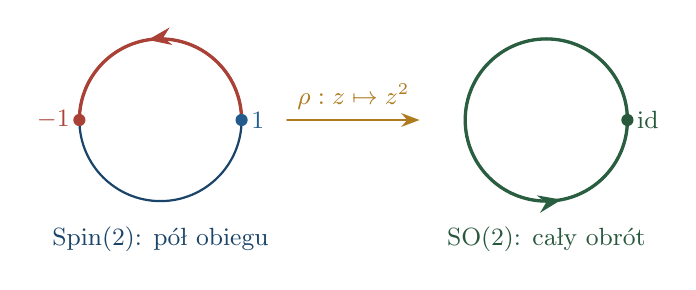
\begin{tikzpicture}[>=Stealth,line cap=round]
 \draw[manifoldblue!75!black,thick] (-2.45,0) circle (1.03);
 \draw[manifoldgreen!75!black,thick] (2.45,0) circle (1.03);
 \draw[manifoldred,very thick,postaction={decorate},
  decoration={markings,mark=at position .55 with {\arrow{Stealth}}}]
  (-1.42,0) arc[start angle=0,end angle=180,radius=1.03];
 \draw[manifoldgreen!75!black,very thick,postaction={decorate},
  decoration={markings,mark=at position .78 with {\arrow{Stealth}}}]
  (3.48,0) arc[start angle=0,end angle=360,radius=1.03];
 \fill[manifoldblue] (-1.42,0) circle (2.2pt)
  node[right,font=\small] {$1$};
 \fill[manifoldred] (-3.48,0) circle (2.2pt)
  node[left,font=\small] {$-1$};
 \fill[manifoldgreen!70!black] (3.48,0) circle (2.2pt)
  node[right,font=\small] {$\id$};
 \draw[->,thick,manifoldgold!85!black] (-.84,0)--(.84,0)
  node[midway,above,font=\small] {$\rho:z\mapsto z^2$};
 \node[font=\small,manifoldblue!75!black] at (-2.45,-1.52)
  {$\operatorname{Spin}(2)$: pół obiegu};
 \node[font=\small,manifoldgreen!70!black] at (2.45,-1.52)
  {$\mathrm{SO}(2)$: cały obrót};
\end{tikzpicture}
\caption{Droga od $1$ do $-1$ w $\operatorname{Spin}(2)$
rzutuje się na pełen obrót w $\mathrm{SO}(2)$.
Końce drogi są różne w grupie Spin, choć odpowiadają
temu samemu obrotowi.}
\label{fig:lin31-spin-dwukrotne}
\end{figure}

\begin{przyklad}[Trzy wymiary: kwaterniony]
\label{prz:lin31-spin3}
W $\operatorname{Cl}(\R^3)$ część parzysta ma bazę
$1,I=e_2e_3,J=e_3e_1,K=e_1e_2$.
Na przykład z \eqref{eq:lin30-cliff-orto}
$I^2=e_2e_3e_2e_3=-e_2^2e_3^2=-1$ oraz
$IJ=e_2e_3e_3e_1=-e_2e_1=e_1e_2=K$.
Cykliczna zamiana indeksów $1,2,3$ daje
$J^2=K^2=-1$, $JK=I$ i $KI=J$.
Iloczyny w odwrotnej kolejności mają przeciwne znaki;
na przykład $JI=e_3e_1e_2e_3=-e_1e_2=-K$.
Jest to algebra kwaternionów $\mathbb H$.
Odwracanie kolejności czynników wysyła
$a+bI+cJ+dK$ na $a-bI-cJ-dK$,
więc $s\widetilde s=a^2+b^2+c^2+d^2$.
Istotnie, dla $q=bI+cJ+dK$ mieszane składniki $q^2$
znikają, bo $IJ+JI=JK+KJ=KI+IK=0$.
Stąd $q^2=-(b^2+c^2+d^2)$ i
$(a+q)(a-q)=a^2-q^2$ daje tę równość.
Każdy element $\operatorname{Spin}(3)$
jest zatem jednostkowym kwaternionem.
I odwrotnie, dowolny jednostkowy kwaternion
można zapisać jako $\cos t+\sin t\,B$,
gdzie $B$ jest jednostkowym dwuwektorem
w $\R^3$ (przypadki $\pm1$ są natychmiastowe).
Każdy taki $B$ jest iloczynem dwóch
prostopadłych wektorów jednostkowych. Aby to sprawdzić,
zapiszmy $B=b e_2e_3+c e_3e_1+d e_1e_2$ z $b^2+c^2+d^2=1$.
Wybierzmy jednostkowy $u\perp n=(b,c,d)$ i połóżmy
$v=n\times u$. Wtedy $u,v$ są ortonormalne i $u\times v=n$.
Współczynniki $u\wedge v$ w bazie
$(e_2\wedge e_3,e_3\wedge e_1,e_1\wedge e_2)$ są właśnie $(b,c,d)$,
więc $uv=B$. Z kolei
$\cos t+\sin t\,B$ jest także iloczynem dwóch
wektorów jednostkowych: jeśli $B=uv$ dla
$u\perp v$, to wprost z $vu=-uv$ i $u^2=-1$
otrzymujemy
\[
 (-\cos t\,u-\sin t\,v)u
     =\cos t+\sin t\,uv.
\]
Zatem $\operatorname{Spin}(3)\cong S^3$
jako grupa jednostkowych kwaternionów,
a $\rho:S^3\to\mathrm{SO}(3)$ utożsamia
parę $s,-s$.
\end{przyklad}

\section{Spinory: moduły algebry Clifforda}
\label{sec:lin31-spinory}

Wektor w $\R^n$ obraca się przez $\rho(s)\in\mathrm{SO}(n)$.
Spinor ma podlegać działaniu samego $s\in\operatorname{Spin}(n)$,
tak aby dwa podniesienia tego samego obrotu mogły
działać odmiennie. Do opisania wszystkich wymiarów
użyjemy liczb zespolonych. \emph{Zespolenie}
$\operatorname{Cl}^{\C}_n:=
\operatorname{Cl}(\R^n)\otimes_\R\C$
ma tę samą bazę uporządkowanych słów co algebra
rzeczywista, ale współczynniki zespolone.
Jego wymiar nad $\C$ wynosi $2^n$.

\begin{definicja}[Spinor zespolony]
\index{spinor zespolony@Spinor zespolony}
\label{def:lin31-spinor}
\emph{Moduł} algebry $A$ nad $\mathbb K$ to przestrzeń liniowa
$\Delta$ nad $\mathbb K$ z działaniem $A\times\Delta\to\Delta$
dwuliniowym nad $\mathbb K$ i zgodnym
z mnożeniem: $(ab)\psi=a(b\psi)$
oraz $1\psi=\psi$. Jest \emph{nieredukowalny},
jeśli $\Delta\ne0$ i nie ma właściwej niezerowej podprzestrzeni
zachowywanej przez wszystkie działania $a\in A$.
W tym rozdziale \emph{przestrzenią spinorów}
w wymiarze $n$ nazwiemy nieredukowalny zespolony
moduł $\Delta_n$ algebry $\operatorname{Cl}^{\C}_n$.
Jej element $\psi$ to spinor. Ograniczenie
działania do $\operatorname{Spin}(n)\subset
\operatorname{Cl}^{\C}_n$ jest
\emph{reprezentacją spinową}.
\end{definicja}

Słowo \emph{moduł} brzmi abstrakcyjnie, lecz tutaj
oznacza po prostu konkretne macierze $c(v)$
działające na kolumny $\psi$, z warunkiem
$c(v)^2=-\|v\|^2 I$. Działanie na całej algebrze
jest wtedy wyznaczone przez jej własność uniwersalną.
Przykładem modułu jest $\Lambda V$ z dowodu
Twierdzenia~\ref{thm:lin30-cliff-baza}, ale zwykle jest
on \emph{większy} niż nieredukowalna przestrzeń
spinorów. Nie należy więc utożsamiać automatycznie
wielowektora ze spinorem.

\begin{przyklad}[Macierze Pauliego]
\label{prz:lin31-pauli}
Niech
\[
 \sigma_1=\begin{pmatrix}0&1\\1&0\end{pmatrix},
 \quad
 \sigma_2=\begin{pmatrix}0&-i\\i&0\end{pmatrix},
 \quad
 \sigma_3=\begin{pmatrix}1&0\\0&-1\end{pmatrix}.
\]
Kwadraty $\sigma_1,\sigma_3$ są identycznością,
a dla $\sigma_2$ dwa diagonalne współczynniki kwadratu
to $(-i)i=i(-i)=1$, przy zerowych pozostałych.
Trzy niezależne iloczyny różnych macierzy wynoszą
\[
 \begin{aligned}
 \sigma_1\sigma_2&=\begin{pmatrix}i&0\\0&-i\end{pmatrix}
                  =i\sigma_3,\\
 \sigma_2\sigma_3&=\begin{pmatrix}0&i\\i&0\end{pmatrix}
                  =i\sigma_1,\\
 \sigma_3\sigma_1&=\begin{pmatrix}0&1\\-1&0\end{pmatrix}
                  =i\sigma_2.
 \end{aligned}
\]
Każda $\sigma_j$ jest hermitowska.
Sprzężenie tych trzech równości daje więc iloczyny w odwrotnej
kolejności: $(\sigma_i\sigma_j)^*=\sigma_j\sigma_i$,
a $(i\sigma_k)^*=-i\sigma_k$.
Otrzymaliśmy $\sigma_i^2=I_2$ oraz
$\sigma_i\sigma_j=-\sigma_j\sigma_i$ dla $i\ne j$.
Macierze $c(e_j)=i\sigma_j$ spełniają więc
\[
 c(e_i)c(e_j)+c(e_j)c(e_i)=-2\delta_{ij}I_2.
\]
Dla $n=2$ wystarczą $c(e_1),c(e_2)$.
Ich iloczyn to $-i\sigma_3$, a cztery macierze
$I_2,i\sigma_1,i\sigma_2,-i\sigma_3$
są liniowo niezależne i rozpinają
$M_2(\C)$. Aby sprawdzić niezależność, przyrównujemy
ich kombinację do macierzy zerowej:
\[
 \alpha I_2+\beta i\sigma_1+\gamma i\sigma_2-\delta i\sigma_3
 =\begin{pmatrix}
   \alpha-i\delta&i\beta+\gamma\\
   i\beta-\gamma&\alpha+i\delta
  \end{pmatrix}=0.
\]
Dodanie i odjęcie równań diagonalnych daje
$\alpha=\delta=0$, a pozostałych $\beta=\gamma=0$.
W przestrzeni wymiaru $4$ te cztery macierze tworzą więc bazę.
Z wymiaru $4$ obu stron dostajemy
$\operatorname{Cl}^{\C}_2\cong M_2(\C)$.
Przestrzeń spinorów $\Delta_2=\C^2$
jest zwykłą przestrzenią kolumn długości $2$.
\end{przyklad}

\begin{twierdzenie}[Klasyfikacja zespolona i wymiar spinorów]
\label{thm:lin31-cliff-kompleks}
Dla $m\geq0$ istnieją izomorfizmy algebr
\begin{align}
 \operatorname{Cl}^{\C}_{2m}
   &\cong M_{2^m}(\C), \label{eq:lin31-cliff-complex-even}\\
 \operatorname{Cl}^{\C}_{2m+1}
   &\cong M_{2^m}(\C)\oplus M_{2^m}(\C).
   \label{eq:lin31-cliff-complex-odd}
\end{align}
Wobec tego nieredukowalny moduł zespolony
ma wymiar $2^{\lfloor n/2\rfloor}$.
Dla parzystego $n$ jest jeden taki moduł
z dokładnością do izomorfizmu, a dla
nieparzystego $n$ są dwa.
\end{twierdzenie}
\begin{proof}
W wymiarze $0$ algebra ma postać $\C$.
W wymiarze $1$ składa się z $a+be_1$ przy
$e_1^2=-1$. Homomorfizm
$a+be_1\mapsto(a+bi,a-bi)$ powstaje przez podstawienia
$e_1=i$ i $e_1=-i$.
Ma odwrotność
$(z_+,z_-)\mapsto(z_++z_-)/2+(z_+-z_-)\,e_1/(2i)$,
więc daje $\operatorname{Cl}^{\C}_1\cong\C\oplus\C$.
Przykład~\ref{prz:lin31-pauli} daje
$\operatorname{Cl}^{\C}_2\cong M_2(\C)$.

Wykażmy krok indukcyjny zwiększający wymiar o $2$.
Iloczyn tensorowy algebr wyposażamy tu w mnożenie
$(a\otimes A)(b\otimes B)=ab\otimes AB$, rozszerzone
dwuliniowo; własność uniwersalna iloczynu tensorowego zapewnia
jego poprawne określenie. Łączność sprawdzamy na tensorach
prostych, a jedynką jest $1\otimes I_2$.
Niech $e_1,\ldots,e_n$ będą generatorami
$\operatorname{Cl}^{\C}_n$. W algebrze
$\operatorname{Cl}^{\C}_n\otimes M_2(\C)$
weźmy $n+2$ elementów:
\[
 F_j=e_j\otimes\sigma_3\ (j\leq n),\qquad
 F_{n+1}=1\otimes i\sigma_1,\qquad
 F_{n+2}=1\otimes i\sigma_2.
\]
Każdy $F_j^2=-1$. Dwa różne elementy
antykomutują: dla $j,\ell\leq n$ wynika
to z relacji starych $e_j$; między pierwszymi
$n$ a ostatnimi dwoma wynika z tego, że
$\sigma_3$ antykomutuje z $\sigma_1,\sigma_2$;
ostatnie dwa antykomutują jako macierze Pauliego.
Własność uniwersalna daje homomorfizm
\[
 \operatorname{Cl}^{\C}_{n+2}
    \longrightarrow
   \operatorname{Cl}^{\C}_n\otimes M_2(\C).
\]
Obrazy dwóch ostatnich generatorów dają całą
podalgebrę $1\otimes M_2(\C)$:
ich iloczyn jest $-i(1\otimes\sigma_3)$,
a wraz z jedynką tworzą bazę czterech macierzy.
Następnie z
$(e_j\otimes\sigma_3)(1\otimes\sigma_3)
=e_j\otimes I_2$ otrzymujemy wszystkie
generatory pierwszego czynnika. Homomorfizm
jest więc surjektywny. Obie algebry mają
wymiar $2^{n+2}$ nad $\C$
(Twierdzenie~\ref{thm:lin30-cliff-baza}),
więc jest izomorfizmem. Używamy przy tym
$M_d(\C)\otimes M_2(\C)\cong M_{2d}(\C)$:
jednostka macierzowa $E_{ab}\otimes E_{rs}$ odpowiada
jednostce z indeksem wiersza $(a,r)$ i kolumny $(b,s)$.
To bijekcja baz zachowująca mnożenie. Iloczyn tensorowy
rozdziela się też względem sumy prostej obu składników.
Iteracja od $n=0$
i $n=1$ daje~\eqref{eq:lin31-cliff-complex-even}
i~\eqref{eq:lin31-cliff-complex-odd}.

Pozostaje uzasadnić wymiary modułów. Algebra
$M_d(\C)$ działa na $\C^d$ nieredukowalnie:
jeśli podprzestrzeń zawiera $x\ne0$, to
dla dowolnego $y\in\C^d$ można znaleźć
macierz $A$ z $Ax=y$, więc zawiera wszystkie $y$.
Każdy nieredukowalny moduł $M_d(\C)$ jest
izomorficzny z tym standardowym: wybieramy
wektor $\psi$ z $E_{11}\psi\ne0$ (w razie potrzeby
zmieniamy indeks; jest to możliwe, gdyż
$\sum_jE_{jj}=I$). Wektory
$E_{i1}\psi$, $1\leq i\leq d$, są liniowo
niezależne: zastosowanie $E_{1j}$ do ich
kombinacji liniowej zerowej pozostawia
tylko $j$-ty współczynnik razy
$E_{11}\psi\ne0$. Ich rozpiętość zachowują
wszystkie macierze, bo
$E_{ab}(E_{i1}\psi)=\delta_{bi}E_{a1}\psi$.
Jest zatem niezerowym podmodułem, a
nieredukowalność wymusza, że stanowi cały moduł.
Dla sumy dwóch algebr macierzowych jej
dwa centralne idempotenty $(I,0)$, $(0,I)$
rozkładają każdy moduł na dwie niezmiennicze
części. W module nieredukowalnym tylko jedna
z nich jest niezerowa, co daje dokładnie
dwa wybory modułu wymiaru $d$.
\end{proof}

\begin{uwaga}[Dwa moduły w wymiarze nieparzystym]
Gdy $n=2m+1\geq3$, dwa nieredukowalne moduły
$\operatorname{Cl}^{\C}_n$ są różne, lecz
po ograniczeniu do $\operatorname{Spin}(n)$
dają izomorficzne reprezentacje.
Rzeczywiście, podalgebra parzysta jest
izomorficzna z
$\operatorname{Cl}^{\C}_{n-1}$: przypiszmy
jego generatorowi $e_j$ element $e_je_n$
dla $j<n$. Dla $j,\ell<n$ obliczamy
$(e_je_n)(e_\ell e_n)=-e_je_\ell e_n^2=e_je_\ell$.
Dla $j=\ell$ daje to kwadrat $-1$, a dla $j\ne\ell$
zamiana $j,\ell$ zmienia znak. Te elementy zatem antykomutują i
generują wszystkie parzyste słowa
(każde $e_je_\ell$ z $j,\ell<n$ jest dokładnie
iloczynem $(e_je_n)(e_\ell e_n)$). Obie strony mają
wymiar $2^{n-1}$, więc to izomorfizm.
Ponieważ $n-1=2m$, algebra parzysta jest
$M_{2^m}(\C)$ i ma tylko jeden nieredukowalny
moduł. Trzeba jeszcze sprawdzić nieredukowalność ograniczeń:
każdy z dwóch modułów ma wymiar $d=2^m$, a w dowolnym
niezerowym module $M_d(\C)$ konstrukcja z jednostkami $E_{ij}$
z poprzedniego dowodu daje podmoduł wymiaru $d$.
Tutaj musi on być całą przestrzenią. Ponadto słowa parzyste
z wektorów ortonormalnych należą do Spin i rozpinają algebrę
parzystą, więc niezmienniczość względem Spin jest równoważna
niezmienniczości względem tej algebry.
W szczególności spinor dla obrotów
wymiaru $3$ ma po prostu dwie zespolone składowe.
Można zobaczyć oba działania Clifforda na tej samej przestrzeni:
jeśli $c_+(v)$ jest jednym z nich, to $c_-(v)=-c_+(v)$
na wektorach. Zmiana znaku każdego słowa nieparzystego
zamienia dwa nieredukowalne moduły, natomiast na słowach
parzystych, a więc i na grupie Spin, działania są identyczne.
Rozróżnia je centralny element
$i^{m+1}e_1\cdots e_{2m+1}$.
Przeniesienie generatora przez $2m$ pozostałych nie zmienia
znaku, co wyjaśnia centralność.
Kwadrat iloczynu $n$ różnych generatorów to
$(-1)^{n(n-1)/2}(-1)^n=(-1)^{n(n+1)/2}$:
pierwszy znak pochodzi od ich uporządkowania, drugi od kwadratów.
Dla $n=2m+1$ wynosi $(-1)^{m+1}$.
Czynnik $i^{m+1}$ ma kwadrat również równy $(-1)^{m+1}$,
więc cały element ma kwadrat $1$.
Zmiana znaków nieparzystej liczby generatorów zmienia jego znak
i zamienia wartości własne.
\end{uwaga}

\begin{stwierdzenie}[Spinory chiralne w wymiarze parzystym]
\label{prop:lin31-spin-chiral}
Dla $n=2m\geq2$ ustalmy orientację $V$ i dodatnią bazę
ortonormalną $(e_1,\ldots,e_{2m})$. W module $\Delta_{2m}$
element
\[
 \Gamma:=i^m c(e_1e_2\cdots e_{2m})
\]
ma własność $\Gamma^2=I$, komutuje z działaniem
$\operatorname{Spin}(2m)$ i dzieli przestrzeń
na dwa nieredukowalne, nieizomorficzne podmoduły dla grupy Spin:
\[
 \Delta_{2m}=\Delta^+_{2m}\oplus\Delta^-_{2m},
 \qquad
 \Delta^\pm_{2m}=\ker(\Gamma\mp I),\qquad
 \dim_\C\Delta^\pm_{2m}=2^{m-1}.
\]
Nazywamy je \emph{półspinorami}.
\end{stwierdzenie}
\begin{proof}
Niech $\omega=e_1\cdots e_{2m}$. Aby uporządkować czynniki
w iloczynie $\omega^2$, wykonujemy $(2m)(2m-1)/2$ transpozycji;
następnie mnożymy $2m$ kwadratów $e_j^2=-1$.
Otrzymujemy
$\omega^2=(-1)^{m(2m-1)}(-1)^{2m}=(-1)^m$.
Ponieważ $i^{2m}=(-1)^m$, mamy $\Gamma^2=I$.
Zatem $P_\pm=\tfrac12(I\pm\Gamma)$ są projekcjami
o sumie $I$ i zerowym iloczynie; dają podany rozkład na przestrzenie własne.
Zmiana dodatniej bazy ortonormalnej nie zmienia $\omega$.
Istotnie, wyrażenie
\[
 \operatorname{Alt}(v_1,\ldots,v_{2m})
 :=\frac{1}{(2m)!}
   \sum_{\pi\in S_{2m}}\operatorname{sgn}(\pi)\,
    v_{\pi(1)}\cdots v_{\pi(2m)}
\]
jest naprzemienne i wieloliniowe, a na bazie ortonormalnej
równa się jej iloczynowi Clifforda, bo wszystkie różne
wektory bazy antykomutują. Jako odwzorowanie naprzemienne
przy zmianie bazy mnoży się przez wyznacznik, tutaj równy $1$.
Przy odwróceniu orientacji $\Gamma$ zmienia znak i oznaczenia
$\Delta^+$, $\Delta^-$ zamieniają się miejscami.
Przesunięcie dowolnego $e_j$ przez pozostałe
$2m-1$ generatory zmienia znak:
$\Gamma c(e_j)=-c(e_j)\Gamma$.
Przez liniowość to samo zachodzi dla $c(v)$ każdego $v\in V$,
więc mnożenie Clifforda przez wektor zamienia oba półspinory.
Zatem $\Gamma$ komutuje z iloczynami
parzystej liczby generatorów, w szczególności
ze $\operatorname{Spin}(2m)$; obie przestrzenie
własne są niezmiennicze. Operator
$c(e_1)$ jest odwracalny i przestawia
te przestrzenie własne, więc mają równe
wymiary. Suma wymiarów to $2^m$ z poprzedniego
twierdzenia, co daje $2^{m-1}$.

Sprawdźmy jeszcze nieredukowalność względem grupy Spin.
Jeśli $0\ne W\subset\Delta^+_{2m}$ jest jej niezmienniczą
podprzestrzenią, to $W\oplus c(e_1)W$ jest niezmiennicza
względem każdego $c(e_j)$: istotnie,
$c(e_1)^{-1}c(e_j)$ oraz $c(e_j)c(e_1)$ są działaniami
elementów Spin (dla $j=1$ pierwszy z nich to $I$).
Stąd $c(e_j)W\subset c(e_1)W$ i
$c(e_j)c(e_1)W\subset W$.
Przestrzeń ta jest więc niezerowym podmodułem całej algebry
Clifforda. Nieredukowalność $\Delta_{2m}$ wymusza
$W\oplus c(e_1)W=\Delta_{2m}$, skąd $W=\Delta^+_{2m}$.
Tak samo postępujemy dla $\Delta^-_{2m}$.
Wreszcie $\omega=e_1\cdots e_{2m}\in\operatorname{Spin}(2m)$
działa na tych przestrzeniach przez różne skalary
$i^{-m}$ i $-i^{-m}$. Żaden niezerowy operator splatający
oba działania grupy Spin nie może więc istnieć.
\end{proof}

\begin{przyklad}[Półspinory w płaszczyźnie]
Dla $n=2$ w modelu Pauliego
$\Gamma=i\,c(e_1)c(e_2)=\sigma_3$,
więc $\Delta^+_2=\C\binom10$ oraz
$\Delta^-_2=\C\binom01$.
Element $s_\theta$ z Przykładu~\ref{prz:lin31-spin2}
działa przez
$c(s_\theta)=\cos(\theta/2)I_2
+\sin(\theta/2)c(e_1)c(e_2)
=\cos(\theta/2)I_2-i\sin(\theta/2)\sigma_3$.
Ponieważ $\sigma_3=\operatorname{diag}(1,-1)$,
oba współczynniki diagonalne to
$\cos(\theta/2)\mp i\sin(\theta/2)=e^{\mp i\theta/2}$.
Zatem
\[
 c(s_\theta)=
 \begin{pmatrix}
  e^{-i\theta/2}&0\\0&e^{i\theta/2}
 \end{pmatrix}.
\]
Wektor po obrocie o $2\pi$ wraca do swego
położenia, a każdy z obu półspinorów
zostaje przemnożony przez $-1$.
\end{przyklad}

\begin{przyklad}[Spinor w $\R^3$ i sfera Blocha]
\label{prz:lin31-bloch}
W wymiarze $3$ działanie
$c(e_j)=i\sigma_j$ na $\Delta_3=\C^2$
spełnia relacje Clifforda. Na parzystych
generatorach z Przykładu~\ref{prz:lin31-spin3}
otrzymujemy macierze $-i\sigma_1,-i\sigma_2,
-i\sigma_3$. Dla
$s=a+bI+cJ+dK\in\operatorname{Spin}(3)$
macierz działania ma postać
\[
 U_s=aI_2-i(b\sigma_1+c\sigma_2+d\sigma_3).
\]
Połóżmy $H=b\sigma_1+c\sigma_2+d\sigma_3$.
Macierze Pauliego są hermitowskie, więc $H^*=H$.
W rozwinięciu $H^2$ składniki mieszane kasują się parami,
bo $\sigma_j\sigma_k+\sigma_k\sigma_j=0$ dla $j\ne k$,
a $\sigma_j^2=I_2$. Stąd
\[
 U_s^*U_s=(aI_2+iH)(aI_2-iH)
 =a^2I_2+H^2=(a^2+b^2+c^2+d^2)I_2=I_2.
\]
Podstawiając macierze Pauliego, dostajemy również
\[
 U_s=\begin{pmatrix}a-id&-c-ib\\c-ib&a+id\end{pmatrix},
 \qquad
 \det U_s=(a^2+d^2)-(-c^2-b^2)=1.
\]
Sprawdźmy teraz, że tak otrzymujemy każdą macierz $U\in\mathrm{SU}(2)$.
Jej pierwsza kolumna $(\alpha,\gamma)^T$ ma normę $1$,
a jednostkowe wektory do niej prostopadłe to
$\lambda(-\overline\gamma,\overline\alpha)^T$, $|\lambda|=1$.
Druga kolumna ma więc tę postać. Wyznacznik takiej macierzy
wynosi $\lambda(|\alpha|^2+|\gamma|^2)=\lambda$,
zatem warunek $\det U=1$ wymusza $\lambda=1$.
Pisząc $\beta=-\overline\gamma$, otrzymujemy
$U=\begin{psmallmatrix}\alpha&\beta\\
-\overline\beta&\overline\alpha\end{psmallmatrix}$,
gdzie $|\alpha|^2+|\beta|^2=1$.
Porównanie współczynników daje jednoznacznie
$a=\Re\alpha$, $d=-\Im\alpha$,
$c=-\Re\beta$, $b=-\Im\beta$;
warunek normy kolumny to właśnie $a^2+b^2+c^2+d^2=1$.
Zatem $\operatorname{Spin}(3)\cong\mathrm{SU}(2)$.

Niech teraz $\psi=(z_1,z_2)^T$ ma normę $1$.
Liczby rzeczywiste
\begin{equation}\label{eq:lin31-spin-bloch}
 b_j(\psi):=\psi^*\sigma_j\psi
 \quad\text{dają}\quad
 b(\psi)=
 \bigl(2\Re(\overline z_1z_2),
       2\Im(\overline z_1z_2),
       |z_1|^2-|z_2|^2\bigr).
\end{equation}
Wyprowadźmy te współrzędne. Dla $w=\overline z_1z_2$
mnożenie przez $\sigma_1$ daje
$\psi^*\sigma_1\psi=w+\overline w=2\Re w$,
a przez $\sigma_2$ daje
$\psi^*\sigma_2\psi=-iw+i\overline w=2\Im w$.
Macierz diagonalna $\sigma_3$ daje różnicę kwadratów modułów.
Ponieważ $(\Re w)^2+(\Im w)^2=|w|^2$, mamy
\[
 \begin{aligned}
 \|b(\psi)\|^2
 &=4|z_1|^2|z_2|^2+(|z_1|^2-|z_2|^2)^2\\
 &=(|z_1|^2+|z_2|^2)^2=1.
 \end{aligned}
\]
Zmiana fazy $\psi\mapsto e^{i\varphi}\psi$
nie zmienia $b(\psi)$: w każdym iloczynie
$\overline z_jz_k$ czynniki fazowe się skracają.
Odwrotnie, liczby $b_j$ wyznaczają macierz
\[
 \begin{aligned}
 \psi\psi^*
 &=\begin{pmatrix}
 |z_1|^2&z_1\overline z_2\\
 z_2\overline z_1&|z_2|^2
 \end{pmatrix}\\
 &=\frac12\begin{pmatrix}
 1+b_3&b_1-ib_2\\b_1+ib_2&1-b_3
 \end{pmatrix}
 =\frac12\left(I_2+\sum_{j=1}^3b_j\sigma_j\right).
 \end{aligned}
\]
Jest to rzut ortogonalny na $\C\psi$: wysyła $v$ na
$\psi(\psi^*v)$ i zachowuje $\psi$, bo $\psi^*\psi=1$.
Jego obraz wyznacza zatem tę prostą jednoznacznie.
Każdy punkt sfery otrzymujemy: dla
$b=(x,y,z)$ z $z>-1$ bierzemy
$z_1=\sqrt{(1+z)/2}$,
$z_2=(x+iy)/\sqrt{2(1+z)}$;
dla bieguna południowego bierzemy $(0,1)$.
Istotnie, $x^2+y^2=1-z^2$ daje
$|z_2|^2=(x^2+y^2)/(2(1+z))=(1-z)/2$,
więc $|z_1|^2+|z_2|^2=1$ oraz $|z_1|^2-|z_2|^2=z$.
Ponadto $\overline z_1z_2=(x+iy)/2$,
co odtwarza dwie pierwsze współrzędne we wzorze~\eqref{eq:lin31-spin-bloch}.
Otrzymujemy więc konkretną identyfikację
\[
 \mathbb{CP}^1=\operatorname{Gr}_1(\C^2)\cong S^2.
\]
Jest to także gładka identyfikacja: na mapie $[1:w]$
wybieramy jednostkowego przedstawiciela
$\psi=(1,w)^T/\sqrt{1+|w|^2}$.
Podstawienie go do~\eqref{eq:lin31-spin-bloch} daje
$b=(2\Re w,2\Im w,1-|w|^2)/(1+|w|^2)$,
a odwrotność poza biegunem południowym to $w=(x+iy)/(1+z)$;
druga mapa analogicznie obsługuje biegun południowy.
Macierze $U_s$ obracają odpowiedni punkt sfery.
Istotnie, z $U_sc(v)U_s^{-1}=c(\rho(s)v)$ i $c(v)=i\sum_jv_j\sigma_j$
otrzymujemy
\[
 (U_s\psi)(U_s\psi)^*
 =U_s\psi\psi^*U_s^{-1}
 =\tfrac12\bigl(I_2+\textstyle\sum_j(\rho(s)b(\psi))_j\sigma_j\bigr).
\]
Jednoznaczność współczynników przy $\sigma_j$ daje
$b(U_s\psi)=\rho(s)b(\psi)$.
Znak spinora $\psi\mapsto-\psi$ jest
niewidoczny po przejściu do punktu sfery.
\end{przyklad}

\begin{figure}[!htbp]
\centering
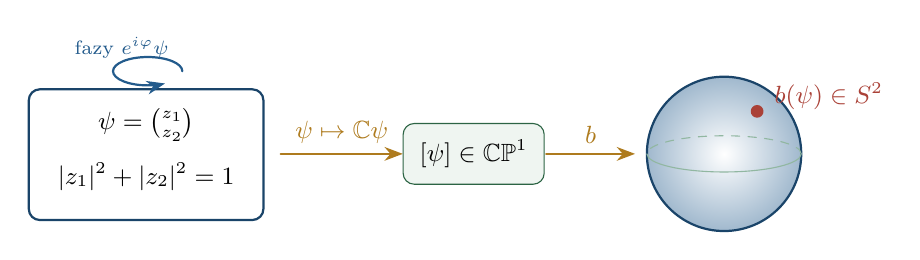
\begin{tikzpicture}[>=Stealth,line cap=round,scale=1.0]
 \draw[manifoldblue!75!black,thick,rounded corners]
 (-5.6,-.72) rectangle (-2.62,.94);
 \node[font=\small] at (-4.11,.49)
   {$\psi=\binom{z_1}{z_2}$};
 \node[font=\small] at (-4.11,-.17)
   {$|z_1|^2+|z_2|^2=1$};
 \draw[->,manifoldblue,thick] (-3.65,1.17)
  arc[start angle=0,end angle=300,x radius=.44,y radius=.18];
 \node[font=\scriptsize,manifoldblue] at (-4.42,1.47)
  {fazy $e^{i\varphi}\psi$};
 \draw[->,thick,manifoldgold!85!black] (-2.4,.12)--(-.85,.12)
  node[midway,above,font=\small] {$\psi\mapsto\C\psi$};
 \node[draw=manifoldgreen!80!black,rounded corners,
  fill=manifoldgreen!8,font=\small,inner sep=6pt] at (.05,.12)
  {$[\psi]\in\mathbb{CP}^1$};
 \draw[->,thick,manifoldgold!85!black] (.97,.12)--(2.1,.12)
  node[midway,above,font=\small] {$b$};
 \shade[inner color=white,outer color=manifoldblue!43] (3.23,.12) circle (.98);
 \draw[manifoldblue!75!black,thick] (3.23,.12) circle (.98);
 \draw[manifoldgreen!55,thin] (2.25,.12)
   arc[start angle=180,end angle=360,x radius=.98,y radius=.23];
 \draw[manifoldgreen!55,thin,dashed] (4.21,.12)
   arc[start angle=0,end angle=180,x radius=.98,y radius=.23];
 \fill[manifoldred] (3.65,.66) circle (2.3pt);
 \node[manifoldred,font=\small] at (4.56,.85) {$b(\psi)\in S^2$};
\end{tikzpicture}
\caption{Spinor jednostkowy $\psi\in\C^2$ ma fazę,
która nie zmienia prostej $[\psi]\in\mathbb{CP}^1$.
Wzór~\eqref{eq:lin31-spin-bloch} przypisuje tej prostej
punkt sfery. To łączy spinory z grassmannianem prostych.}
\label{fig:lin31-spin-bloch}
\end{figure}

\section{Struktury spinowe i wiązki spinorów}
\label{sec:lin31-struktura-spinowa}

Dotąd wektory, obroty i spinory należały do jednej
ustalonej przestrzeni $\R^n$. Na rozmaitości
przestrzeń $T_pM$ zmienia się z $p$.
Gładka rodzina dodatnio określonych iloczynów
skalarnych $g_p$ na $T_pM$ to \emph{metryka
riemannowska}. Pozwala wybierać bazy ortonormalne
w każdym punkcie. Jeśli $M$ jest zorientowana,
możemy wybierać bazy o dodatniej orientacji.

\emph{Wiązka dodatnio zorientowanych ramek
ortonormalnych} $F^+(M)\to M$ ma w punkcie $p$
za włókno wszystkie uporządkowane bazy
$(u_1,\ldots,u_n)$ przestrzeni $T_pM$,
które są ortonormalne i dodatnie.
Grupa $\mathrm{SO}(n)$ działa z prawej strony
przez zmianę takiej bazy. Nie ma wyróżnionej
bazy w każdym włóknie; lokalnie wiązka wygląda
jednak jak $U\times\mathrm{SO}(n)$.
Wiązkę o takiej lokalnej postaci, z wolnym
działaniem grupy przechodzącym tranzytywnie
na każdym włóknie, nazywamy \emph{wiązką główną}.

\begin{definicja}[Struktura spinowa i wiązka spinorowa]
\index{struktura spinowa i wiazka spinorowa@Struktura spinowa i wiązka spinorowa}
\label{def:lin31-struktura-spinowa}
Dla zorientowanej rozmaitości riemannowskiej
$M^n$, $n\geq2$, \emph{struktura spinowa}
składa się z wiązki głównej
$P_{\mathrm{Spin}}\to M$ o grupie
$\operatorname{Spin}(n)$ oraz odwzorowania
gładkiego $\lambda:P_{\mathrm{Spin}}\to F^+(M)$
nad identycznością bazy, takiego że
\[
 \lambda(pg)=\lambda(p)\rho(g),
 \qquad g\in\operatorname{Spin}(n),
\]
a $\lambda$ ograniczona do każdego włókna
jest dwukrotnym nakryciem.
Niech $\varrho:\operatorname{Spin}(n)\to\operatorname{GL}(\Delta_n)$
będzie ograniczeniem działania modułu Clifforda do grupy Spin.
\emph{Wiązka spinorowa} to wiązka zespolona
\[
 S:=P_{\mathrm{Spin}}\times_{\varrho}\Delta_n.
\]
Jej elementami są klasy par $(p,\psi)$,
$p\in P_{\mathrm{Spin}}$, $\psi\in\Delta_n$,
z relacją $(pg,\psi)\sim(p,\varrho(g)\psi)$.
\emph{Polem spinorowym} nazywamy gładki przekrój $S$.
Tę samą definicję stosujemy do dowolnej zorientowanej wiązki
euklidesowej $E$ rzędu $n$, zastępując $F^+(M)$ wiązką jej
dodatnich ramek ortonormalnych $F^+(E)$.
\end{definicja}

Po wyborze lokalnej ramki spinowej $s_i:U_i\to P_{\mathrm{Spin}}$
wiązka $S$ wygląda jak $U_i\times\Delta_n$. Ustalmy kierunek
zmian: jeśli $s_j=s_i h_{ij}$, to
$[s_j,\psi_j]=[s_i,c(h_{ij})\psi_j]$, zatem współrzędne
tego samego spinora spełniają $\psi_i=c(h_{ij})\psi_j$.
Przy przejściu od kolumny $i$ do kolumny $j$ używamy więc
macierzy odwrotnej. Z równości dla lokalnych ramek wynika też
$h_{ij}h_{jk}=h_{ik}$; reprezentacja $c$ przenosi tę równość
na macierze przejścia, co uzasadnia strukturę wiązki wektorowej $S$.
Wiązka spinorów ma ponadto \emph{mnożenie Clifforda przez wektory
styczne}. Dla $v\in T_xM$, $p\in(P_{\mathrm{Spin}})_x$ i
ramki $\lambda(p)$ traktowanej jako izometria
$f_p:\R^n\to T_xM$ określmy
\begin{equation}\label{eq:lin31-spin-bundle-cliff}
 c_x(v)[p,\psi]
   :=[p,c(f_p^{-1}v)\psi].
\end{equation}
Sprawdźmy niezależność od reprezentanta klasy. Gdy $p'=pg$,
to $f_{p'}=f_p\rho(g)$, a $[p',\psi']=[p,c(g)\psi']$.
Oznaczając $w=f_p^{-1}v$, dostajemy
\[
 [p',c(f_{p'}^{-1}v)\psi']
 =[p,c(g)c(\rho(g)^{-1}w)\psi']
 =[p,c(w)c(g)\psi'].
\]
Druga równość wynika z relacji
$c(g)c(u)c(g)^{-1}=c(\rho(g)u)$.
Zatem wzór~\eqref{eq:lin31-spin-bundle-cliff} jest dobrze określony,
zależy gładko od $x$ i spełnia
$c_x(v)^2=-g_x(v,v)I_{S_x}$.
W wymiarze parzystym $\Gamma$ jest niezmienniczy przy zmianie
dodatniej ramki, więc definiuje globalny rozkład
$S=S^+\oplus S^-$; mnożenie przez wektor zamienia $S^+$ z $S^-$.
Gdy chce się mnożyć przez kowektory, najpierw używa się metryki
do identyfikacji $T_x^*M\cong T_xM$.
W przypadku ogólnej wiązki $E$ w tym samym wzorze zastępujemy
$T_xM$ przez $E_x$.
W nieparzystym wymiarze dwa wybory nieredukowalnego działania
Clifforda dają równoważne działanie Spin na $S$, lecz w tym
utożsamieniu zmieniają znak mnożenia przez pojedynczy wektor.
Zauważmy też, że $\lambda$ jest nakryciem całych przestrzeni:
w lokalnej trywializacji zadanej przez $s_i$ i ramkę $\lambda\circ s_i$
ma postać $(x,g)\mapsto(x,\rho(g))$.
Jeśli zmiana ramki wektorowej wykonuje pełny
obrót o $2\pi$, jej podniesienie w Spin
może dojść do $-1$. Wtedy wektory wracają
do wartości początkowych, lecz spinor dostaje
znak minus. To lokalna treść różnicy między
wiązką wektorów i wiązką spinorów.

\begin{przyklad}[Płaszczyzna i sfera są spinowe]
Na $\R^n$ standardowe ramki dają
$F^+(\R^n)\cong\R^n\times\mathrm{SO}(n)$.
Bierzemy
$P_{\mathrm{Spin}}=\R^n\times\operatorname{Spin}(n)$
i $\lambda(x,s)=(x,\rho(s))$; spinory
tworzą trywialną wiązkę
$S\cong\R^n\times\Delta_n$.

Na sferze $S^2\subset\R^3$ każda dodatnia
ramka styczna $(u,v)$ w punkcie $p$ wyznacza
macierz o kolumnach $(u,v,p)\in\mathrm{SO}(3)$.
To utożsamia $F^+(S^2)$ z $\mathrm{SO}(3)$,
a rzut do bazy wysyła macierz na jej trzecią
kolumnę $p$. Dwukrotne nakrycie
$\mathrm{SU}(2)\cong\operatorname{Spin}(3)
\to\mathrm{SO}(3)$ z
Przykładu~\ref{prz:lin31-spin3} daje odwzorowanie $\lambda$.
Rzut z $\operatorname{Spin}(3)$ do sfery ma postać
$q(s)=\rho(s)e_3$. Używamy jednej, ustalonej podgrupy
$H=\rho^{-1}(\operatorname{Stab}(e_3))=\operatorname{Spin}(2)$,
złożonej z $\cos t+\sin t\,e_1e_2$. Działa ona z prawej strony
na $\operatorname{Spin}(3)$ i zachowuje $q(s)$.
Jeśli $q(s)=q(s')$, to $s^{-1}s'\in H$, więc działanie jest
wolne i przechodnie na każdym włóknie. Lokalne gładkie ramki
styczne $(u,v)$ dają lokalne sekcje w $\mathrm{SO}(3)$;
po zmniejszeniu otoczenia podnosimy je przez lokalną odwrotność
nakrycia $\rho$. To zapewnia lokalną trywialność wiązki głównej.
Równość $\lambda(sh)=\lambda(s)\rho(h)$ kończy sprawdzenie
definicji struktury spinowej na sferze.
\end{przyklad}

\begin{przyklad}[Cztery podniesienia ramek płaskiego torusa]
\label{prz:lin31-spin-torus}
Niech $T^2=\R^2/\Z^2$ ma metrykę płaską i orientację
zadaną przez stałą ramkę $(\partial_x,\partial_y)$.
W tej ramce $F^+(T^2)\cong T^2\times\mathrm{SO}(2)$.
Dla każdej pary znaków
$\varepsilon=(\varepsilon_1,\varepsilon_2)\in\{1,-1\}^2$
grupa $\Z^2$ działa na $\R^2\times\operatorname{Spin}(2)$ wzorem
\[
 (k_1,k_2)\cdot(x,s)
  =\bigl(x+(k_1,k_2),
          \varepsilon_1^{k_1}\varepsilon_2^{k_2}s\bigr).
\]
Iloraz $P_\varepsilon$ jest wiązką główną Spin:
nad małym kwadratem w torusie wybór jego podniesienia do $\R^2$
daje lokalną trywializację, a znaki są centralne,
więc działanie grupy Spin z prawej strony schodzi na iloraz.
Odwzorowanie
$\lambda_\varepsilon[x,s]=([x],\rho(s))$
jest dobrze określone, gdyż $\rho(\pm1)=I$.
Na każdym włóknie jest dwukrotnym nakryciem, zatem daje
strukturę spinową. Para $\varepsilon$ zapisuje znaki,
z jakimi podniesienie ustalonej stałej ramki wraca
po obejściu dwóch podstawowych pętli torusa.

Te cztery struktury są różne jako \emph{podniesienia}
ustalonej wiązki ramek. Istotnie, izomorfizm
$P_\varepsilon\to P_{\varepsilon'}$ zgodny z $\lambda$
po podciągnięciu do $\R^2$ ma postać
$(x,s)\mapsto(x,\delta(x)s)$, gdzie
$\delta(x)\in\ker\rho=\{\pm1\}$.
Funkcja $\delta$ jest stała, bo $\R^2$ jest spójna.
Porównanie identyfikacji punktów przy przesunięciach
o $(1,0)$ i $(0,1)$ wymusza więc
$\varepsilon_1=\varepsilon'_1$ oraz
$\varepsilon_2=\varepsilon'_2$.

Są to wszystkie struktury spinowe na torusie. Dla dowolnego
podniesienia $P\to F^+(T^2)$ podciągamy je do $\R^2$ i bierzemy
przeciwobraz stałej ramki. Jest to dwukrotne nakrycie
ściągalnej $\R^2$, więc ma gładką sekcję $\widetilde f$.
Po przesunięciu o $k\in\Z^2$ jej wartości nad tym samym
punktem torusa różnią się znakiem $\delta_k(x)\in\{\pm1\}$.
Ciągłość i spójność $\R^2$ czynią ten znak stałym w $x$,
a składanie przesunięć daje homomorfizm
$k\mapsto\delta_k$ z $\Z^2$ do $\{\pm1\}$.
Wyznaczają go dwa znaki dla $(1,0)$ i $(0,1)$;
trywializacja $(x,s)\mapsto\widetilde f(x)s$ utożsamia
wyjściowe podniesienie z odpowiednim $P_\varepsilon$.

W trywializacji spinorów podciągniętej do $\R^2$
pole spinorowe jest funkcją $\psi:\R^2\to\Delta_2$
spełniającą konkretne warunki
\[
 \psi(x+1,y)=\varepsilon_1\psi(x,y),
 \qquad
 \psi(x,y+1)=\varepsilon_2\psi(x,y).
\]
Wyprowadźmy te warunki z relacji ilorazowej.
Dla $k=(k_1,k_2)\in\Z^2$ oznaczmy
$\varepsilon^k=\varepsilon_1^{k_1}\varepsilon_2^{k_2}$.
Ramki spinowe nad tym samym punktem spełniają
$[x+k,1]=[x,\varepsilon^k]$.
W wiązce stowarzyszonej zastąpienie ramki $p$ przez $p h$
zastępuje współrzędną spinora przez $c(h)^{-1}$ razy tę współrzędną.
Zapis tego samego pola w obu ramkach wymaga więc
$\psi(x)=c(\varepsilon^k)\psi(x+k)$.
Z $c(-1)=-I_{\Delta_2}$ mamy
$c(\varepsilon^k)=\varepsilon^k I_{\Delta_2}$;
ponieważ $(\varepsilon^k)^2=1$, dostajemy
$\psi(x+k)=\varepsilon^k\psi(x)$.
Wybory $k=(1,0)$ i $k=(0,1)$ dają oba wypisane warunki.
Wybór znaku $-1$ oznacza więc antyperiodyczność
w odpowiednim kierunku, choć zwykłe wektory styczne
są okresowe w obu kierunkach.
\end{przyklad}

\begin{figure}[!htbp]
\centering
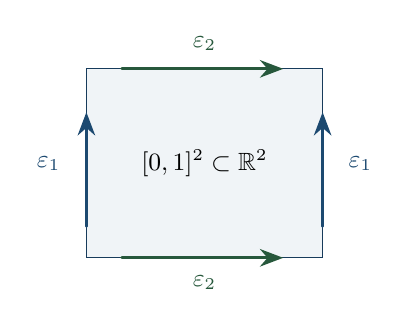
\begin{tikzpicture}[>=Stealth,line cap=round]
 \fill[manifoldblue!7] (0,0) rectangle (3,2.4);
 \draw[manifoldblue!65!black,thin] (0,0) rectangle (3,2.4);
 \draw[->,manifoldblue!80!black,very thick]
   (0,.4)--(0,1.85);
 \draw[->,manifoldblue!80!black,very thick]
   (3,.4)--(3,1.85);
 \draw[->,manifoldgreen!70!black,very thick]
   (.45,0)--(2.5,0);
 \draw[->,manifoldgreen!70!black,very thick]
   (.45,2.4)--(2.5,2.4);
 \node[font=\small,manifoldblue!80!black] at (-.48,1.2)
   {$\varepsilon_1$};
 \node[font=\small,manifoldblue!80!black] at (3.48,1.2)
   {$\varepsilon_1$};
 \node[font=\small,manifoldgreen!70!black] at (1.5,-.32)
   {$\varepsilon_2$};
 \node[font=\small,manifoldgreen!70!black] at (1.5,2.72)
   {$\varepsilon_2$};
 \node[font=\small] at (1.5,1.2) {$[0,1]^2\subset\R^2$};
\end{tikzpicture}
\caption{Dwie pary brzegów kwadratu fundamentalnego torusa.
Przesunięcie w kierunku $x$ utożsamia pionowe krawędzie
ze znakiem $\varepsilon_1$ dla spinora; przesunięcie w kierunku
$y$ utożsamia poziome krawędzie ze znakiem $\varepsilon_2$.
W wiązce ramek ortonormalnych oba znaki są niewidoczne.}
\label{fig:lin31-spin-torus-signs}
\end{figure}

\begin{uwaga}[Podnoszenie na zbiorze ściągalnym]
\label{rem:lin31-spin-podnoszenie}
Użyjemy elementarnego faktu o nakryciach: gładkie odwzorowanie
ze ściągalnego obszaru $U$ do podstawy gładkiego nakrycia ma
gładkie podniesienie po wybraniu obrazu jednego punktu.
Istotnie, drogę od tego punktu podnosimy kolejno przez lokalne
odwrotności nakrycia, dzieląc jej przedział parametrów na skończenie
wiele odcinków. Jednoznaczność na przecięciach daje jednoznaczność
podniesionej drogi. Homotopię dróg o ustalonych końcach podnosimy
analogicznie po podziale kwadratu parametrów na małe prostokąty,
których obrazy leżą w dziedzinach lokalnych odwrotności.
Końcowy punkt podniesienia nie zmienia się w tej homotopii:
poruszałby się ciągle w dyskretnym włóknie. W obszarze ściągalnym
każde dwie drogi o tych samych końcach są tak homotopijne,
więc ich podniesienia wyznaczają tę samą wartość w punkcie końcowym.
Otrzymana funkcja jest lokalnie złożeniem danej funkcji z jedną
lokalną odwrotnością nakrycia, zatem jest gładka.
Ten sam argument działa na dysku z brzegiem.
\end{uwaga}

\begin{przyklad}[Wiązka, której nie da się podnieść]
\label{prz:lin31-nie-spin-linia}
Podłoże $S^2\cong\mathbb{CP}^1$ jest spinowe,
ale nie każda \emph{wiązka} nad nim dopuszcza
podniesienie struktury do Spin.
Weźmy zespoloną wiązkę tautologiczną
$\gamma^1_\C$ nad
$\operatorname{Gr}_1(\C^2)=\mathbb{CP}^1$
i potraktujmy jej włókna jako rzeczywiste
zorientowane płaszczyzny wymiaru $2$.
Na mapie $[1:z]$ mamy ramkę zespoloną
$s_0(z)=(1,z)$, a na mapie $[w:1]$,
$w=1/z$, ramkę $s_\infty(w)=(w,1)$.
Na przecięciu
$s_\infty(1/z)=z^{-1}s_0(z)$.
Po unormowaniu ramek, przy $|z|=1$, $z=e^{i\theta}$, unitarny
czynnik przejścia jest więc $e^{-i\theta}$:
jako rzeczywista izometria obraca płaszczyznę
o kąt $-\theta$. Po przejściu
$0\leq\theta\leq2\pi$ daje pętlę
o nieparzystej liczbie pełnych obrotów.
Ta pętla w $\mathrm{SO}(2)$ nie ma
\emph{zamkniętego} podniesienia do $\operatorname{Spin}(2)$:
połowa kąta biegnie
od $0$ do $-\pi$ i kończy w $-1$, nie w $1$.
Gdyby istniała struktura spinowa, ramkę ortonormalną nad każdą
z dwóch półkul można by podnieść do ramki spinowej.
Rzeczywiście, przeciwobraz takiej ramki przez $\lambda$ jest
dwukrotnym nakryciem dysku; Uwagi~\ref{rem:lin31-spin-podnoszenie}
używamy do podniesienia identyczności dysku. Przejście między
otrzymanymi ramkami spinowymi na równiku byłoby właśnie
zamkniętym podniesieniem opisanej pętli, co jest sprzecznością.
Zmiana ramki na którejś z dwóch półkul
zmienia pętlę tylko o taką, która przedłuża
się na dysk i ma zerowy całkowity obrót.
Dlatego ten brak podniesienia nie zależy
od wybranych ramek. Wiązka rzeczywista otrzymana przez zapomnienie
struktury zespolonej $\gamma^1_\C$ nie ma struktury
spinowej, mimo że sama sfera $S^2$ ją ma.
\end{przyklad}

\begin{stwierdzenie}[Znaki na potrójnych przecięciach]
\label{prop:lin31-w2-znaki}
Niech $E$ będzie zorientowaną wiązką euklidesową
rzędu $n\geq2$ nad $M$. Weźmy dostatecznie drobne
pokrycie trywializujące $(U_i)$, w którym
niepuste skończone przecięcia są ściągalne. Takie pokrycie
nazywamy \emph{dobrym}; w tym stwierdzeniu jawnie zakładamy jego istnienie i wybór.
Niech $g_{ij}:U_i\cap U_j\to\mathrm{SO}(n)$
przepisują współrzędne z trywializacji $j$ do trywializacji $i$,
więc $g_{ij}g_{jk}=g_{ik}$.
Na przecięciach wybierzmy podniesienia
$h_{ij}:U_i\cap U_j\to\operatorname{Spin}(n)$
z $\rho(h_{ij})=g_{ij}$ i $h_{ji}=h_{ij}^{-1}$.
Wtedy na potrójnym przecięciu
\begin{equation}\label{eq:lin31-w2-znaki}
 \varepsilon_{ijk}:=h_{ij}h_{jk}h_{ki}
          \in\{1,-1\}.
\end{equation}
Wiązka $E$ ma strukturę spinową dokładnie wtedy,
gdy wybory $h_{ij}$ można zmodyfikować znakami
tak, aby wszystkie $\varepsilon_{ijk}$ wynosiły $1$.
\end{stwierdzenie}
\begin{proof}
Z warunku kocyklu dla $g_{ij}$ mamy
$\rho(\varepsilon_{ijk})
=g_{ij}g_{jk}g_{ki}=I$.
Twierdzenie~\ref{thm:lin31-spin-nakrycie} mówi, że
jądro $\rho$ to $\{\pm1\}$; ponieważ znak jest
dyskretny, $\varepsilon_{ijk}$ jest lokalnie stały.
Nie ma problemu z samym podniesieniem
$g_{ij}$ na ściągalnym przecięciu:
zapewnia je Uwaga~\ref{rem:lin31-spin-podnoszenie}.
Przyjmujemy też $h_{ii}=1$.

Jeżeli na każdym potrójnym przecięciu
$\varepsilon_{ijk}=1$, to
$h_{ij}h_{jk}=h_{ik}$.
Są to funkcje przejścia z warunkiem kocyklu.
Sklejamy $U_i\times\operatorname{Spin}(n)$ relacją
$(x,a)_j\sim(x,h_{ij}(x)a)_i$. Warunek kocyklu zapewnia
przechodniość tej relacji, a gładkie przejścia definiują lokalne
trywializacje. Istotnie, na każdym $U_i$ klasy
$[x,a]_i$ tworzą kopię $U_i\times\operatorname{Spin}(n)$,
a na przecięciu zmiana tej kopii jest gładkim
odwzorowaniem $(x,a)\mapsto(x,h_{ij}(x)a)$.
Jest to ta sama konstrukcja sklejania, której
użyto dla wiązek wektorowych
w Sekcji~\ref{sec:lin29-grass-styczna}.
Działanie z prawej strony jest dobrze określone, wolne
i przechodnie we włóknach, więc otrzymujemy wiązkę główną.
Jeśli $f_i$ oznacza wybraną lokalną ramkę $E$, to
$\lambda([x,a]_i)=f_i(x)\rho(a)$ jest niezależne od reprezentanta,
ponieważ $f_j=f_i g_{ij}$ i $\rho(h_{ij})=g_{ij}$.
Lokalnie jest to $\id\times\rho$, a więc spełnia definicję
struktury spinowej.
Odwrotnie, w istniejącej strukturze spinowej podnosimy każdą
ustaloną ramkę $f_i$ do ramki spinowej nad ściągalnym $U_i$.
Stosujemy Uwagę~\ref{rem:lin31-spin-podnoszenie} do dwukrotnego
nakrycia będącego przeciwobrazem $f_i$ przez $\lambda$.
Przejścia tych ramek podnoszą właśnie dane $g_{ij}$ i spełniają
warunek kocyklu, więc wszystkie znaki są $1$.
Dowolne dwa odwzorowania $h_{ij}$ nad
tym samym $g_{ij}$ różnią się na spójnym
przecięciu stałym znakiem
$\delta_{ij}\in\{\pm1\}$.
Zmiana podniesień zastępuje
$\varepsilon_{ijk}$ przez
$\delta_{ij}\delta_{jk}\delta_{ki}
\varepsilon_{ijk}$, co dowodzi
sformułowania o modyfikacji znakami.
\end{proof}

\begin{uwaga}[Druga klasa Stiefela--Whitneya]
Zdarza się, że pojedynczych znaków
$\varepsilon_{ijk}$ nie da się wszystkich
usunąć. Ich układ spełnia warunek zgodności
na poczwórnych przecięciach. Z definicji znaków mamy
$h_{ij}h_{jk}=\varepsilon_{ijk}h_{ik}$.
Stosując tę równość do dwóch sposobów nawiasowania
iloczynu trzech przejść, otrzymujemy
\[
 \begin{aligned}
 (h_{ij}h_{jk})h_{k\ell}
 &=\varepsilon_{ijk}h_{ik}h_{k\ell}
 =\varepsilon_{ijk}\varepsilon_{ik\ell}h_{i\ell},\\
 h_{ij}(h_{jk}h_{k\ell})
 &=h_{ij}\varepsilon_{jk\ell}h_{j\ell}
 =\varepsilon_{jk\ell}\varepsilon_{ij\ell}h_{i\ell}.
 \end{aligned}
\]
W drugim wierszu użyto centralności znaku $\varepsilon_{jk\ell}$.
Łączność mnożenia i skrócenie odwracalnego $h_{i\ell}$
dają $\varepsilon_{ijk}\varepsilon_{ik\ell}
=\varepsilon_{jk\ell}\varepsilon_{ij\ell}$.
Taką rodzinę znaków nazywamy
\emph{dwukocyklowym} zapisem przeszkody.
Zmiany przez $\delta_{ij}$ z dowodu
uznajemy za równoważne. Nie zmienia tego wybór lokalnych ramek:
jeśli $f'_i=f_i a_i$, wybieramy podniesienia $b_i$ funkcji $a_i$
nad ściągalnymi $U_i$. Wtedy $g'_{ij}=a_i^{-1}g_{ij}a_j$
mają podniesienia $h'_{ij}=b_i^{-1}h_{ij}b_j$.
Ich iloczyn na potrójnym przecięciu to
$b_i^{-1}\varepsilon_{ijk}b_i=\varepsilon_{ijk}$,
bo znaki należą do centrum grupy Spin.
Wyjaśnijmy używane tutaj oznaczenie kohomologiczne,
aby nie odsyłać definicji przeszkody wyłącznie do
późniejszej teorii kohomologii. Utożsamiamy
$\{1,-1\}$ z grupą addytywną $\Z/2$ przez
$(-1)^a\longleftrightarrow a$.
Dla dobrego pokrycia $\mathcal U=(U_i)$
niech $C^q(\mathcal U;\Z/2)$ oznacza grupę rodzin
$a_{i_0\ldots i_q}\in\Z/2$, przypisanych
wszystkim niepustym przecięciom
$U_{i_0}\cap\cdots\cap U_{i_q}$ z rosnącymi indeksami.
Definiujemy \emph{operator kobrzegu}
$\delta:C^q(\mathcal U;\Z/2)\to C^{q+1}(\mathcal U;\Z/2)$ wzorem
\[
 (\delta a)_{i_0\ldots i_{q+1}}
 =\sum_{r=0}^{q+1}
 a_{i_0\ldots\widehat{i_r}\ldots i_{q+1}}
 \pmod 2.
\]
Każdy wyraz powstający przez pominięcie dwóch
różnych indeksów występuje w $\delta^2 a$ dwukrotnie,
a $1+1=0$ w $\Z/2$; zatem $\delta^2=0$.
Daje to dobrze określoną grupę
\[
 H^2(\mathcal U;\Z/2)
 :=\frac{\ker(\delta:C^2\to C^3)}
          {\operatorname{im}(\delta:C^1\to C^2)}.
\]
Jeśli $\varepsilon_{ijk}=(-1)^{a_{ijk}}$,
sprawdzona wyżej tożsamość na poczwórnych
przecięciach staje się
$(\delta a)_{ijk\ell}=0$, więc $a$ jest
\emph{dwukocyklem}. Zastąpienie
$h_{ij}$ przez $(-1)^{b_{ij}}h_{ij}$
zmienia go na $a+\delta b$:
na potrójnym przecięciu nowy wykładnik
wynosi $a_{ijk}+b_{ij}+b_{jk}+b_{ik}$
modulo $2$. Klasa $[a]$ jest więc niezależna
od wyboru podniesień, a $[a]=0$ dokładnie wtedy,
gdy można usunąć wszystkie znaki, otrzymując
funkcje przejścia struktury spinowej.

Dla dobrego pokrycia standardowe twierdzenie
o kohomologii Čech utożsamia powyższą grupę
z $H^2(M;\Z/2)$, niezależnie od wyboru
dobrego pokrycia. Otrzymana klasa
$w_2(E):=[a]\in H^2(M;\Z/2)$
jest \emph{drugą klasą Stiefela--Whitneya}.
Z udowodnionego kryterium wynika
\[
 E\text{ ma strukturę spinową}
 \quad\Longleftrightarrow\quad w_2(E)=0
\]
dla zorientowanej wiązki euklidesowej
rzędu co najmniej $2$ nad rozpatrywaną
rozmaitością. Samo utożsamienie różnych
dobrych pokryć z kohomologią przestrzeni jest
twierdzeniem z późniejszej teorii; test znaku
i jego niezależność od podniesień dowiedliśmy tutaj.
Dla wiązki z
Przykładu~\ref{prz:lin31-nie-spin-linia}
przeszkoda jest niezerowa.
\end{uwaga}

\subsection{Pola spinorowe i zmiana ramki}
\label{sec:lin31-pola-spinorowe-podstawy}
\index{pole spinorowe}

Definicja~\ref{def:lin31-struktura-spinowa} rozróżnia spinor
$\psi(x)\in S_x$ w jednym punkcie od pola spinorowego,
czyli gładkiego przekroju $\psi\in\Gamma^\infty(S)$.
Lokalne kolumny pola sklejają się według reprezentacji
spinowej, jak wyprowadzono po tej definicji.
Dalej oznaczamy tę samą wiązkę także przez $S(M)$.
\begin{stwierdzenie}[Pola jako odwzorowania ekwiwariantne]
\label{prop:lin31-pola-spinorowe-ekwiwariantnosc}
Niech $n\geq2$, niech $(M^n,g)$ będzie zorientowaną
rozmaitością riemannowską ze strukturą spinową
$P_{\mathrm{Spin}}\to M$, a $S(M)$ stowarzyszoną
wiązką spinorową określoną przez reprezentację
$\varrho:\operatorname{Spin}(n)\to\operatorname{GL}(\Delta_n)$.
Istnieje naturalna bijekcja między
$\Gamma^\infty(S(M))$ a zbiorem gładkich odwzorowań
$F:P_{\mathrm{Spin}}\to\Delta_n$ spełniających
\begin{equation}\label{eq:lin31-pola-spinorowe-ekwiwariantnosc}
 F(ph)=\varrho(h)^{-1}F(p),\qquad
 h\in\operatorname{Spin}(n),\quad p\in P_{\mathrm{Spin}}.
\end{equation}
\end{stwierdzenie}
\begin{proof}
Dla pola $\psi$ i ramki spinowej $p$ nad $x$ istnieje
jedyny $z\in\Delta_n$ taki, że $\psi(x)=[p,z]$;
kładziemy $F(p)=z$. Przejście do $ph$ wymusza
$F(ph)=\varrho(h)^{-1}F(p)$. Odwrotnie, dla takiego $F$
przypisanie $x\mapsto[p,F(p)]$ nie zależy od wyboru
ramki nad $x$ i wyznacza gładki przekrój.
\end{proof}

\begin{uwaga}[Ramki ortonormalne a ramki spinowe]
\label{rem:lin31-pola-spinorowe-ramki}
Niech na przecięciu $e_j=e_i A_{ij}$ oznacza zmianę
lokalnej ramki ortonormalnej, gdzie $A_{ij}$ jest
odwzorowaniem o wartościach w $\mathrm{SO}(n)$,
a $h_{ij}$ jego podniesieniem do $\operatorname{Spin}(n)$.
Współrzędne wektora stycznego transformują się jako
$v_j=A_{ij}^{-1}v_i$, natomiast współrzędne spinora
jako $\psi_j=\varrho(h_{ij})^{-1}\psi_i$.
Są to działania różnych reprezentacji. W szczególności
wektor nie staje się spinorem tylko dlatego, że zapisano go
w postaci kolumny współrzędnych.
\end{uwaga}

\begin{center}
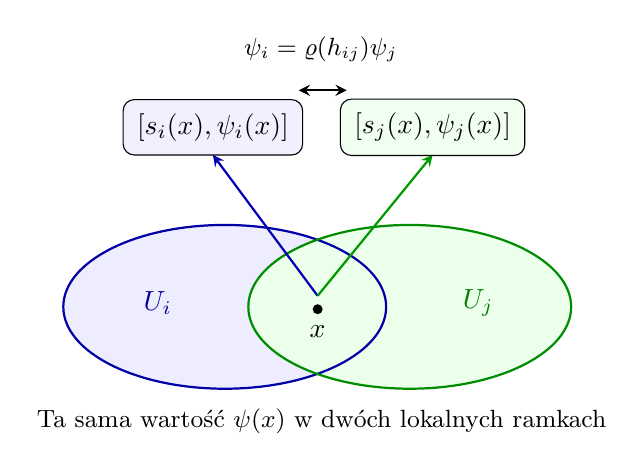
\begin{tikzpicture}[>=stealth,scale=1]
 \fill[blue!7] (-4.7,-1.1) ellipse (2.05 and 1.04);
 \fill[green!8] (-2.35,-1.1) ellipse (2.05 and 1.04);
 \draw[blue!65!black,thick] (-4.7,-1.1) ellipse (2.05 and 1.04);
 \draw[green!55!black,thick] (-2.35,-1.1) ellipse (2.05 and 1.04);
 \fill[black] (-3.52,-1.13) circle (1.8pt);
 \node[below] at (-3.52,-1.22) {$x$};
 \node[blue!60!black] at (-5.55,-1.05) {$U_i$};
 \node[green!50!black] at (-1.48,-1.05) {$U_j$};
 \draw[->,thick,blue!70!black] (-3.52,-.96)--(-4.85,.83);
 \draw[->,thick,green!60!black] (-3.52,-.96)--(-2.06,.83);
 \node[draw,rounded corners,fill=blue!6,align=center,inner sep=5pt]
  at (-4.85,1.18) {$[s_i(x),\psi_i(x)]$};
 \node[draw,rounded corners,fill=green!6,align=center,inner sep=5pt]
  at (-2.06,1.18) {$[s_j(x),\psi_j(x)]$};
 \draw[<->,thick] (-3.76,1.65)--(-3.15,1.65);
 \node[font=\small] at (-3.48,2.17)
  {$\psi_i=\varrho(h_{ij})\psi_j$};
 \node[font=\small] at (-3.47,-2.55)
  {Ta sama wartość $\psi(x)$ w dwóch lokalnych ramkach};
\end{tikzpicture}

{\small\itshape Dwie lokalne reprezentacje jednego pola spinorowego.
Warunek sklejania zapewnia zgodność na przecięciu obszarów.}
\end{center}

Różniczkowanie pól spinorowych wymaga dodatkowego
wyboru koneksji na $S(M)$. Jej konstrukcja przez
koneksję Levi-Civity oraz lokalne prawa transformacji
należą do geometrii różniczkowej; tutaj ograniczamy się
do algebraicznej i wiązkowej struktury spinorów.


\par\smallskip
{\footnotesize\noindent\emph{Dalsza lektura:}
Rachunki z konwencją $v^2=-\|v\|^2$
można porównać z notatkami Briana Conrada,
\emph{Clifford algebras and spin groups},
\url{https://math.stanford.edu/~conrad/210CPage/handouts/clifford.pdf}.
Budowę struktur spinowych i opis przeszkody
$w_2$ rozwijają notatki Konstantina Wernliego,
\emph{Lecture Notes on Spin Geometry},
\url{https://arxiv.org/pdf/1911.09766}.
Obie lektury używają miejscami innej kolejności tematów.
Powyższy test znaków został dowiedziony bez użycia kohomologii;
jego interpretacja jako klasy w $H^2$ korzysta z teorii
kohomologii Čech, której tutaj nie dowodziliśmy.\par}
\clearpage

\chapter{Twistory: spinory, incydencja i fibracja nad sferą}
\label{ch:lin32-twistory}
\index{twistor}
Rozdział~\ref{ch:lin31-spinory} wprowadził spinory i ich reprezentacje.
Teraz pokażemy, jak algebra liniowa spinorów prowadzi do geometrii
twistorowej. W modelu zespolonym punkt przestrzeni czterowymiarowej
odpowiada prostej rzutowej w $\mathbb{CP}^3$. W modelu euklidesowym
nad każdym punktem $S^4$ znajduje się taka prosta, będąca włóknem
gładkiej fibracji. Konstrukcje te mają tę samą przestrzeń rzutową,
lecz korzystają z różnych dodatkowych struktur. Rozróżnienie
obu modeli jest istotne.

\section{Macierze $2\times2$ jako wektory czterowymiarowe}
\label{sec:lin32-macierze}
Ustalmy dwie dwuwymiarowe zespolone przestrzenie $S_+$ i $S_-$
z wybranymi bazami. Ich przestrzeń homomorfizmów
$V_{\C}:=\operatorname{Hom}_{\C}(S_-,S_+)$
utożsamiamy z $M_2(\C)$. Odpowiada to dwóm typom
spinorów chiralnych z Rozdziału~\ref{ch:lin31-spinory},
lecz samo utożsamienie wymaga wyboru baz.

\begin{definicja}[Forma kwadratowa wyznacznika]
\label{def:lin32-forma}
Dla $X=\begin{psmallmatrix}a&b\\c&d\end{psmallmatrix}$
określamy $q(X)=\det X=ad-bc$ i jego polaryzację
$B(X,Y)=q(X+Y)-q(X)-q(Y)$.
Niezerową macierz $X$ nazywamy \emph{izotropową},
gdy $q(X)=0$. Punkty $X,Y$ nazywamy
\emph{rozdzielonymi izotropowo}, gdy $q(X-Y)=0$.
\end{definicja}

\begin{stwierdzenie}[Niezdegenerowanie i działanie grup]
\label{prop:lin32-dzialanie}
Forma $B$ jest niezdegenerowana.
Grupa $\mathrm{SL}_2(\C)\times\mathrm{SL}_2(\C)$ działa na
$V_{\C}$ przez $(A,D)\cdot X=AXD^{-1}$, zachowując $q$.
Jądro tego działania to
$\{(I_2,I_2),(-I_2,-I_2)\}$.
\end{stwierdzenie}
\begin{proof}
Dla $Y=\begin{psmallmatrix}a'&b'\\c'&d'\end{psmallmatrix}$
rozwinięcie wyznacznika daje
$B(X,Y)=ad'+a'd-bc'-b'c$.
Jeśli $B(X,Y)=0$ dla wszystkich $Y$, podstawienie
czterech macierzy jednostkowych $E_{11},E_{22},E_{12},E_{21}$
wymusza kolejno $d=a=c=b=0$.
Z multiplikatywności wyznacznika
$q(AXD^{-1})=(\det A)q(X)(\det D)^{-1}=q(X)$.
Jeśli $(A,D)$ działa trywialnie, to z $X=I_2$
wynika $A=D$. Wtedy $AX=XA$ dla wszystkich $X$.
Komutowanie z $E_{11}$ wymusza diagonalność $A$,
a z $E_{12}$ równość wyrazów diagonalnych.
Stąd $A=\lambda I_2$ i $\lambda^2=\det A=1$.
Obie pary znaków rzeczywiście działają trywialnie.
\end{proof}

\begin{przyklad}[Postać rzeczywista lorentzowska]
\label{prz:lin32-hermit}
Dla rzeczywistych $t,x,y,z$ bierzemy macierz hermitowską
\[
 H(t,x,y,z)=
 \begin{pmatrix}t+z&x-iy\\x+iy&t-z\end{pmatrix}.
\]
Mnożenie liczb zespolonych daje
$\det H=(t+z)(t-z)-(x-iy)(x+iy)=t^2-x^2-y^2-z^2$.
Jest to rzeczywista forma o sygnaturze $(1,3)$.
Nie jest ona euklidesową metryką na $\R^4$:
tę odmienną sytuację rozpatrzymy przy fibracji nad $S^4$.
\end{przyklad}

\section{Kwadryka Segrego i płaszczyzny izotropowe}
\label{sec:lin32-segre}
Każda niezerowa macierz $X$ o $\det X=0$ ma rząd
jeden, więc można ją zapisać jako
$X=u\alpha^{\mathsf T}$ dla niezerowych
$u,\alpha\in\C^2$. Dwa takie przedstawienia
różnią się zastąpieniem $(u,\alpha)$ przez
$(\lambda u,\lambda^{-1}\alpha)$.

\begin{twierdzenie}[Kwadryka Segrego]
\label{thm:lin32-segre}
Odwzorowanie
\[
 \mathrm{Seg}:\mathbb{CP}^1\times\mathbb{CP}^1
 \longrightarrow\mathbb{CP}^3,\qquad
 ([u_0:u_1],[a_0:a_1])
 \longmapsto[u_0a_0:u_0a_1:u_1a_0:u_1a_1]
\]
jest osadzeniem holomorficznym. Jego obrazem jest
kwadryka $Q=\{[z_{11}:z_{12}:z_{21}:z_{22}]:
z_{11}z_{22}-z_{12}z_{21}=0\}$, składająca się
dokładnie z rzutowych klas niezerowych macierzy
izotropowych w $V_{\C}$.
\end{twierdzenie}
\begin{proof}
Skalowanie któregokolwiek czynnika mnoży wszystkie
współrzędne obrazu przez wspólną niezerową liczbę,
więc wzór jest dobrze określony. Jego macierz
ma rząd jeden, a zatem wyznacznik zero.
Na odwrót, każda niezerowa macierz o wyznaczniku
zero ma jednoznacznie określoną prostą obrazu
i prostą przestrzeni wierszy. Te dwie proste
odtwarzają $[u]$ i $[\alpha]$, więc odwzorowanie
jest bijekcją na $Q$.
Na mapach $u_0a_0\ne0$ piszemy $u=(1,s)$,
$\alpha=(1,t)$; wtedy obrazem jest $[1:t:s:st]$.
Jego odwrotność w tej mapie wyznaczają
$s=z_{21}/z_{11}$ i $t=z_{12}/z_{11}$.
Pozostałe trzy pary map otrzymujemy przez
zmianę wyróżnionych niezerowych współrzędnych.
W każdej z nich odwrotność jest holomorficzna,
co dowodzi osadzenia.
\end{proof}

\begin{twierdzenie}[Dwie rodziny maksymalnych płaszczyzn izotropowych]
\label{thm:lin32-rodziny}
Każda dwuwymiarowa podprzestrzeń $L\subset V_{\C}$
spełniająca $q|_L=0$ ma postać
\[
 \{u\alpha^{\mathsf T}:\alpha\in\C^2\}
 \quad\text{lub}\quad
 \{u\alpha^{\mathsf T}:u\in\C^2\},
\]
dla ustalonego niezerowego $u$ albo ustalonego
niezerowego $\alpha$. Są to wszystkie maksymalne
podprzestrzenie izotropowe, parametryzowane
przez dwie kopie $\mathbb{CP}^1$.
\end{twierdzenie}
\begin{proof}
Wybierzmy niezależne
$X=u\alpha^{\mathsf T}$, $Y=v\beta^{\mathsf T}$
rozpinające $L$. Dla każdego $\lambda\in\C$
mamy
\[
 0=\det(X+\lambda Y)
 =\lambda\,\det[u\ v]\,
 \det\begin{pmatrix}\alpha^{\mathsf T}\\
                     \beta^{\mathsf T}\end{pmatrix}.
\]
Zatem albo $u,v$ są proporcjonalne, albo
$\alpha,\beta$ są proporcjonalne.
W pierwszym przypadku wszystkie macierze z $L$
mają tę samą prostą obrazu, a w drugim
tę samą przestrzeń wierszy. Otrzymujemy dwie postacie
z tezy; obie rzeczywiście są podprzestrzeniami
wymiaru dwa i zawierają tylko macierze rzędu
co najwyżej jeden. Jeśli $W$ jest dowolną
izotropową podprzestrzenią, polaryzacja
$q(w+w')=0$ pokazuje, że $B|_{W\times W}=0$,
więc $W\subset W^{\perp_B}$.
Niezdegenerowanie $B$ daje
$\dim W+\dim W^{\perp_B}=4$,
czyli $\dim W\le2$. Udowodniliśmy maksymalność.
\end{proof}

Rzutowanie takich płaszczyzn daje dwie rodziny
prostych leżących na kwadryce $Q$.
W teorii twistorów prowadzi to do dwóch rodzajów
całkowicie izotropowych płaszczyzn, zwanych
często płaszczyznami $\alpha$ i $\beta$.
Z konwencją incydencji poniżej związana będzie
rodzina o ustalonej przestrzeni wierszy.

\section{Twistory i incydencja}
\label{sec:lin32-incydencja}
\begin{definicja}[Przestrzeń twistorów i prosta twistorowa]
\label{def:lin32-twistor}
Niech $\mathbb T=S_+\oplus S_-\cong\C^4$.
Niezerowy \emph{twistor} zapisujemy
$Z=(\omega,\pi)$, $\omega\in S_+$, $\pi\in S_-$.
\emph{Rzutowa przestrzeń twistorów} to
$\mathbb{PT}=\mathbb P(\mathbb T)\cong\mathbb{CP}^3$.
Dla punktu $X\in V_{\C}=M_2(\C)$
\emph{relacja incydencji} ma postać
$\omega=X\pi$ przy $\pi\ne0$.
Odpowiadająca $X$ \emph{prosta twistorowa} to
\[
 \ell_X=\{[X\pi:\pi]:\pi\in\C^2\setminus\{0\}\}
                   \subset\mathbb{PT}.
\]
Konwencja fizyczna $\omega=iX\pi$ powstaje
po zastąpieniu $X$ przez $iX$.
\end{definicja}

Przestrzeń $\{(X\pi,\pi):\pi\in\C^2\}$ jest
dwuwymiarową zespoloną podprzestrzenią $\C^4$,
będącą wykresem odwzorowania liniowego $X$.
Jej rzutowanie jest prostą $\mathbb{CP}^1$.
Dlatego punkt $X$ odpowiada \emph{całej prostej},
a nie jednemu twistorowi.

\begin{twierdzenie}[Przecięcie prostych i izotropowość]
\label{thm:lin32-przeciecie}
Dla dowolnych $X,Y\in M_2(\C)$ zachodzi
\[
 \ell_X\cap\ell_Y\ne\varnothing
 \quad\Longleftrightarrow\quad\det(X-Y)=0.
\]
Dla $X\ne Y$ z zerowym wyznacznikiem różnicy
proste przecinają się w dokładnie jednym punkcie;
dla $X=Y$ pokrywają się.
\end{twierdzenie}
\begin{proof}
Punkt wspólny ma przedstawienia
$[X\pi:\pi]=[Y\eta:\eta]$ z $\pi,\eta\ne0$.
Istnieje więc $\lambda\in\C^\ast$ takie, że
$X\pi=\lambda Y\eta$ i $\pi=\lambda\eta$,
czyli $(X-Y)\pi=0$.
Na odwrót, każdy niezerowy $\pi\in\ker(X-Y)$
daje punkt obu prostych.
Jądro jest niezerowe dokładnie przy
$\det(X-Y)=0$. Gdy $X\ne Y$, macierz różnicy
jest niezerowa o rzędzie jeden, a jej jądro
ma wymiar jeden, więc rzutowo otrzymujemy
dokładnie jeden punkt. Przypadek $X=Y$
jest bezpośredni.
\end{proof}

\begin{przyklad}[Przecięcie i rozłączność]
\label{prz:lin32-przeciecie}
Dla $X=0$ oraz $Y=\operatorname{diag}(1,0)$
różnica ma wyznacznik zero i
$\ker(X-Y)=\C(0,1)^{\mathsf T}$.
Wspólnym twistorem jest $[0:0:0:1]$.
Natomiast dla $X=0$ oraz $Y=I_2$
wyznacznik różnicy wynosi $1$,
więc proste nie mają punktu wspólnego.
\end{przyklad}

\begin{stwierdzenie}[Płaszczyzna incydencji jednego twistoru]
\label{prop:lin32-alfa}
Dla $Z=[\omega:\pi]\in\mathbb{PT}$,
$\pi\ne0$, zbiór
$A_Z=\{X\in M_2(\C):X\pi=\omega\}$
jest afiniczną płaszczyzną zespoloną
wymiaru dwa. Jej przestrzeń kierunkowa
$N_\pi=\{T:T\pi=0\}$ jest całkowicie izotropowa
i należy do rodziny o stałej przestrzeni
wierszy z Twierdzenia~\ref{thm:lin32-rodziny}.
\end{stwierdzenie}
\begin{proof}
Odwzorowanie $L_\pi:M_2(\C)\to\C^2$,
$L_\pi(X)=X\pi$, jest surjektywne:
wybierając $\eta$ tak, aby $(\pi,\eta)$
stanowiło bazę, możemy zadawać dowolnie
$X\pi=\omega$ i $X\eta=0$.
Z twierdzenia o rzędzie i jądrze
$\dim_\C N_\pi=4-2=2$.
Jego każde niezerowe $T$ ma niezerowe
jądro, więc $\det T=0$. Ta sama własność
dotyczy kombinacji liniowych elementów $N_\pi$.
Jeśli niezerowy funkcjonał $\alpha$ ma
$\ker\alpha=\C\pi$, każdy wiersz $T$
jest proporcjonalny do $\alpha$.
Stąd $N_\pi=\{u\alpha:u\in\C^2\}$.
\end{proof}

\begin{przyklad}[Jawna płaszczyzna $\alpha$]
\label{prz:lin32-alfa}
Dla $\pi=(1,0)^{\mathsf T}$,
$\omega=(a,b)^{\mathsf T}$ warunek
$X\pi=\omega$ ustala tylko pierwszą kolumnę:
\[
 A_Z=\left\{\begin{pmatrix}a&s\\b&t\end{pmatrix}
                 :s,t\in\C\right\}.
\]
Każda różnica dwóch takich macierzy
ma pierwszą kolumnę zerową i wyznacznik zero.
\end{przyklad}

\begin{figure}[!htbp]
\centering
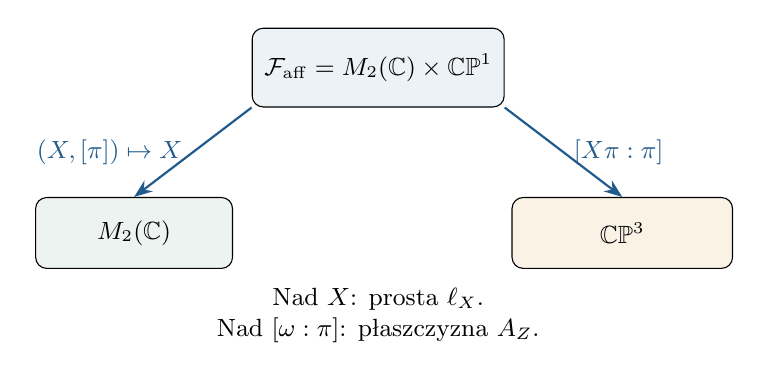
\begin{tikzpicture}[>=Stealth,font=\small]
 \node[draw,rounded corners,fill=manifoldblue!8,
       minimum width=3.2cm,minimum height=1.0cm]
       (F) at (0,2.1)
       {$\mathcal F_{\mathrm{aff}}=M_2(\C)\times\mathbb{CP}^1$};
 \node[draw,rounded corners,fill=manifoldgreen!9,
       minimum width=2.5cm,minimum height=.9cm]
       (M) at (-3.1,0) {$M_2(\C)$};
 \node[draw,rounded corners,fill=manifoldgold!12,
       minimum width=2.8cm,minimum height=.9cm]
       (P) at (3.1,0) {$\mathbb{CP}^3$};
 \draw[->,thick,manifoldblue] (F.south west)--(M.north)
       node[midway,left] {$(X,[\pi])\mapsto X$};
 \draw[->,thick,manifoldblue] (F.south east)--(P.north)
       node[midway,right] {$[X\pi:\pi]$};
 \node[align=center] at (0,-1.05)
       {Nad $X$: prosta $\ell_X$.\\
        Nad $[\omega:\pi]$: płaszczyzna $A_Z$.};
\end{tikzpicture}
\caption{Dwa rzuty korespondencji incydencji.
Punkt przestrzeni macierzy odpowiada prostej twistorowej,
a twistor z $\pi\ne0$ płaszczyźnie afinicznej.}
\label{fig:lin32-incydencja}
\end{figure}

\section{Grassmannian i kwadryka Kleina}
\label{sec:lin32-klein}
Jak w Rozdziale~\ref{ch:lin29-grassmanniany},
$\operatorname{Gr}_2(\C^4)$ parametryzuje
dwuwymiarowe podprzestrzenie $\C^4$.
Punktowi $X$ przypisujemy wykres
$W_X=\{(X\pi,\pi):\pi\in\C^2\}$.
Rzutowanie $W_X\to S_-$ jest izomorfizmem.
Odwrotnie, każda płaszczyzna o takim rzutowaniu
jest wykresem jednoznacznego $X$,
więc $M_2(\C)$ jest otwartą mapą Grassmannianu.

\begin{twierdzenie}[Współrzędne Plückera wykresu]
\label{thm:lin32-plucker}
Przy osadzeniu Plückera
$\operatorname{Gr}_2(\C^4)\hookrightarrow\mathbb{CP}^5$
obrazem jest kwadryka Kleina
\begin{equation}\label{eq:lin32-klein}
 p_{12}p_{34}-p_{13}p_{24}+p_{14}p_{23}=0.
\end{equation}
Dla $X=\begin{psmallmatrix}a&b\\c&d\end{psmallmatrix}$
punkt $W_X$ ma współrzędne
\[
 [p_{12}:p_{13}:p_{14}:p_{23}:p_{24}:p_{34}]
       =[ad-bc:-b:a:-d:c:1].
\]
Część $p_{34}\ne0$ tej kwadryki jest
izomorficzna z $M_2(\C)$.
\end{twierdzenie}
\begin{proof}
Bazą $W_X$ są kolumny
$v_1=(a,c,1,0)^{\mathsf T}$,
$v_2=(b,d,0,1)^{\mathsf T}$.
Wyznaczniki dwuwierszowych minorów
dają kolejno $ad-bc,-b,a,-d,c,1$.
Podstawienie w~\eqref{eq:lin32-klein}
daje $(ad-bc)+bc-ad=0$.
Dla ogólnej płaszczyzny równanie
Plückera zostało dowiedzione w
Twierdzeniu~\ref{thm:lin29-grass-plucker}.
Jeśli $p_{34}\ne0$, dolne dwie
współrzędne pewnej bazy płaszczyzny
tworzą macierz odwracalną.
Zmieniając bazę, sprowadzamy jej dolny
blok do $I_2$ i otrzymujemy dokładnie
płaszczyznę $W_X$ dla jednej macierzy $X$.
\end{proof}

Nie należy mylić dwóch kwadryk:
$Q\subset\mathbb{CP}^3$ z
Twierdzenia~\ref{thm:lin32-segre}
opisuje \emph{izotropowe kierunki}
w $V_{\C}$, podczas gdy czterowymiarowa
kwadryka Kleina w $\mathbb{CP}^5$,
czyli $\operatorname{Gr}_2(\C^4)$,
opisuje rzutowe domknięcie
\emph{przestrzeni punktów} $X$.

\begin{stwierdzenie}[Pełna korespondencja flag]
\label{prop:lin32-flagi}
Niech $\mathcal F$ będzie zbiorem par
$(\ell,W)$ podprzestrzeni $\C^4$
takich, że $\dim\ell=1$, $\dim W=2$,
$\ell\subset W$. Rzut na
$\operatorname{Gr}_2(\C^4)$ ma włókno
$\mathbb{CP}^1$, a rzut na
$\operatorname{Gr}_1(\C^4)=\mathbb{CP}^3$
ma włókno $\mathbb{CP}^2$.
\end{stwierdzenie}
\begin{proof}
Nad ustalonym $W$ wybieramy prostą
$\ell\subset W$, więc włóknem jest
$\mathbb P(W)\cong\mathbb{CP}^1$.
Nad ustalonym $\ell$ każda
płaszczyzna $W\supset\ell$ odpowiada
prostej $W/\ell\subset\C^4/\ell$.
Ponieważ przestrzeń ilorazowa ma
wymiar trzy, jej proste tworzą
$\mathbb{CP}^2$.
Dla $W=W_X$ i $\ell=[\omega:\pi]$
otrzymujemy ponownie incydencję
$\omega=X\pi$, o ile $\pi\ne0$.
\end{proof}

\section{Kwaternionowa struktura na $\C^4$}
\label{sec:lin32-j}
W drugim modelu $\mathbb{CP}^3$ wybieramy
\emph{rzeczywistą strukturę kwaternionową}.
Zapiszmy $\mathbb H=\{a+jb:a,b\in\C\}$,
z $j^2=-1$ i $aj=j\bar a$.
W prawostronnej przestrzeni zespolonej
$\mathbb H\cong\C^2$ prawe mnożenie przez $j$
ma współrzędne
\[
 J_0(a,b)=(-\bar b,\bar a),\qquad
 J_0^2=-\id.
\]
Ostatni wzór wynika po podstawieniu
$J_0(-\bar b,\bar a)=(-a,-b)$.
Na $\C^4\cong\mathbb H^2$ ustalamy
$J=J_0\oplus J_0$.

\begin{lemat}[Rzutowa inwolucja bez punktów stałych]
\label{lem:lin32-rzeczywista}
Dla $z\in\C^4\setminus\{0\}$ wektory
$z,Jz$ są liniowo niezależne,
a $W_z=\operatorname{span}_\C(z,Jz)$
jest $J$-niezmienniczą płaszczyzną.
Odwzorowanie $\jmath([z])=[Jz]$
jest antyholomorficzną inwolucją
$\mathbb{CP}^3$ bez punktów stałych.
\end{lemat}
\begin{proof}
Gdyby $Jz=\lambda z$, to
$-z=J^2z=\bar\lambda Jz=|\lambda|^2z$,
sprzecznie z $z\ne0$.
Niezależność jest więc dowiedziona,
a $J(W_z)=W_z$ wynika z $J(Jz)=-z$.
Dla $\mu\ne0$ mamy
$J(\mu z)=\bar\mu Jz$, więc
$\jmath$ nie zależy od przedstawiciela
projektowego i jest antyholomorficzne.
Równość $[J^2z]=[-z]=[z]$
daje inwolucję, a jej punkt stały
prowadziłby do wykluczonej równości
$Jz=\lambda z$.
\end{proof}

Każda $J$-niezmiennicza zespolona
płaszczyzna wymiaru dwa jest
jednowymiarową prawostronną
podprzestrzenią kwaternionową
w $\mathbb H^2$. Istotnie, jest
zamknięta na mnożenie przez
$\C$ i przez $j$, a więc przez
wszystkie kwaterniony; dowolny
niezerowy $z$ wraz z $Jz$
stanowi jej zespoloną bazę.
Rodzinę tych płaszczyzn oznaczamy
$\mathbb{HP}^1$.

\begin{twierdzenie}[Fibracja twistorowa]
\label{thm:lin32-fibracja}
Odwzorowanie
\begin{equation}\label{eq:lin32-fibracja}
 \tau:\mathbb{CP}^3\longrightarrow\mathbb{HP}^1,
 \qquad \tau([z])=\operatorname{span}_\C(z,Jz)
\end{equation}
jest gładką, surjektywną, lokalnie trywialną
fibracją z włóknem $\mathbb{CP}^1$.
Ponadto $\mathbb{HP}^1$ jest
dyfeomorficzna z $S^4$.
\end{twierdzenie}
\begin{proof}
Z $J(\lambda z)=\bar\lambda Jz$
wynika niezależność od przedstawiciela.
Każda kwaternionowa prosta $W$
ma bazę zespoloną $(z,Jz)$,
więc należy do obrazu $\tau$.
Przeciwobraz $W$ składa się ze wszystkich
zespolonych prostych w $W$,
czyli jest $\mathbb P(W)\cong\mathbb{CP}^1$.

Udowodnijmy gładką lokalną trywialność.
Punkty $\mathbb{HP}^1$ zapisujemy
jako $[q_0:q_1]_{\mathbb H}$, z
$(q_0,q_1)\sim(q_0h,q_1h)$
dla $h\in\mathbb H^\ast$.
W obszarze $q_0\ne0$ współrzędną jest
$q=q_1q_0^{-1}\in\mathbb H$,
a odpowiadająca prosta ma postać
$W_q=\{(v,qv):v\in\mathbb H\}$.
Wybór zespolonej prostej $\C v\subset\mathbb H$
daje trywializację
\[
 (q,[v]_\C)\longmapsto[(v,qv)]_\C
 \quad\text{z }\mathbb H\times\mathbb{CP}^1
 \text{ na }\tau^{-1}(\{q_0\ne0\}).
\]
Wzór jest bijektywny: pierwsza składowa
niezerowego wektora w $W_q$ nie może
być zerem, a jej klasa wyznacza $[v]_\C$.
Dla $q=s+jt$, $v=a+jb$ mnożenie
kwaternionów daje
$qv=(sa-\bar t b)+j(ta+\bar s b)$.
Zatem trywializacja ma współrzędne
\[
 (q,[a:b])\longmapsto
 [a:b:sa-\bar t b:ta+\bar s b].
\]
Jej odwrotność otrzymujemy przez
$q=q_1q_0^{-1}$ i $[v]_\C=[q_0]_\C$
po utożsamieniu pary zespolonej z kwaternionem.
Oba wzory są gładkie w każdej mapie
rzutowej. Nad $q_1\ne0$ postępujemy
symetrycznie.

Pozostaje zidentyfikować podstawę.
Obszar $q_0\ne0$ daje $\mathbb H\cong\R^4$,
a jego dopełnieniem jest jeden punkt
$\infty=[0:1]_{\mathbb H}$.
Dla $q\in\mathbb H$ połóżmy
\[
 \Phi(q)=
 \left(\frac{2q}{1+|q|^2},
       \frac{|q|^2-1}{1+|q|^2}\right)
       \in\mathbb H\oplus\R\cong\R^5.
\]
To punkt $S^4$, ponieważ
$4|q|^2+(|q|^2-1)^2=(1+|q|^2)^2$.
Przy $q\to\infty$ mamy
$\Phi(q)\to(0,1)$.
W drugiej mapie kwaternionowej
współrzędną na przecięciu jest $q^{-1}$;
wzór w tych współrzędnych przedłuża się
gładko przez punkt $\infty$.
Otrzymujemy stereograficzną
dyfeomorficzną identyfikację
$\mathbb{HP}^1\cong S^4$.
\end{proof}

\begin{przyklad}[Dwa jawne włókna]
\label{prz:lin32-wlokna}
Nad punktem $q=0$ mamy
$W_0=\{(v,0):v\in\mathbb H\}$,
więc
$\tau^{-1}(0)=\{[z_0:z_1:0:0]\}\cong\mathbb{CP}^1$.
Nad $\infty$ mamy
$\tau^{-1}(\infty)=\{[0:0:z_2:z_3]\}\cong\mathbb{CP}^1$.
Te proste są rozłączne. Ogólniej,
dwa różne włókna są rozłączne,
ponieważ różne jednowymiarowe
podprzestrzenie kwaternionowe
mają przecięcie $\{0\}$.
\end{przyklad}

\begin{figure}[!htbp]
\centering
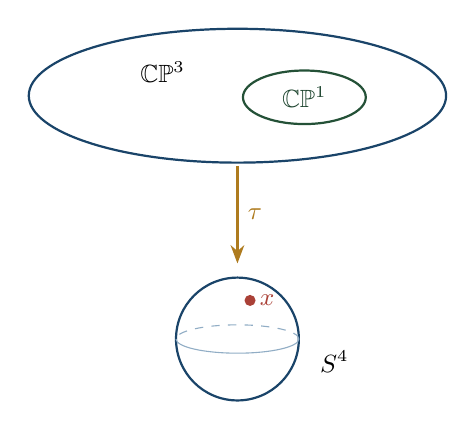
\begin{tikzpicture}[>=Stealth,font=\small]
 \draw[manifoldblue!75!black,thick] (0,2.25)
       ellipse (2.65 and .85);
 \node at (-.95,2.55) {$\mathbb{CP}^3$};
 \draw[manifoldgreen!65!black,thick] (.85,2.23)
       ellipse (.78 and .34);
 \node[manifoldgreen!55!black] at (.85,2.23)
       {$\mathbb{CP}^1$};
 \draw[->,thick,manifoldgold!85!black]
       (0,1.36)--(0,.12) node[midway,right] {$\tau$};
 \draw[manifoldblue!75!black,thick] (0,-.84) circle (.78);
 \draw[manifoldblue!50] (-.78,-.84)
       arc[start angle=180,end angle=360,
       x radius=.78,y radius=.18];
 \draw[manifoldblue!50,dashed] (.78,-.84)
       arc[start angle=0,end angle=180,
       x radius=.78,y radius=.18];
 \fill[manifoldred] (.16,-.35) circle (2pt)
       node[right] {$x$};
 \node at (1.23,-1.13) {$S^4$};
\end{tikzpicture}
\caption{Schemat fibracji twistorowej
$\mathbb{CP}^1\hookrightarrow\mathbb{CP}^3
\xrightarrow{\tau}S^4$. Rysunek nie oznacza,
że całkowita przestrzeń jest globalnym iloczynem.}
\label{fig:lin32-fibracja}
\end{figure}

\begin{uwaga}[Dwa modele, dwie geometrie]
\label{rem:lin32-modele}
Zespolona relacja incydencji pozwala, by
różne proste $\ell_X,\ell_Y$ miały punkt wspólny;
dzieje się tak właśnie wtedy, gdy
$\det(X-Y)=0$. W modelu euklidesowym
różne włókna $\tau^{-1}(x)$ są rozłączne.
Nie utożsamiamy tych dwóch rodzin prostych
bez wyboru odpowiedniej rzeczywistej struktury.
Odwzorowanie $\tau$ jest gładkie,
ale nie nazywamy go holomorficznym:
podstawa $S^4$ nie została wyposażona
w strukturę zespoloną, podczas gdy
$\mathbb{CP}^3$ ma standardową taką strukturę.
\end{uwaga}

\section{Związki z algebrą liniową i dalsze kierunki}
\label{sec:lin32-wnioski}
Podstawowym obiektem obu konstrukcji jest
zespolona przestrzeń $\mathbb T\cong\C^4$
i jej rzutowanie $\mathbb{CP}^3$.
Relacja incydencji wybiera w niej
wykresy $W_X$ macierzy $2\times2$.
Struktura kwaternionowa wybiera zamiast
tego płaszczyzny niezmiennicze względem $J$.

Oba modele prowadzą do Grassmannianu
$\operatorname{Gr}_2(\C^4)$: jest on
przestrzenią \emph{wszystkich} prostych
rzutowych w $\mathbb{CP}^3$.
Jego obraz Plückera to kwadryka Kleina,
a rodzina $J$-niezmienniczych płaszczyzn
odpowiada rzeczywistej podrozmaitości
$\mathbb{HP}^1\cong S^4$.
Macierze rzędu jeden kodują z kolei
dwa typy maksymalnych kierunków
izotropowych, związanych ze spinorami.

Rozwinięcie tych idei do transformacji
Penrose'a, korespondencji Penrose'a--Warda
i analizy pól spinorowych wymaga teorii
snopów, kohomologii oraz koneksji.
Nie wynika ono automatycznie z dowiedzionych
tu elementarnych twierdzeń o incydencji
i fibracji.

\par\smallskip
{\footnotesize\noindent\emph{Dalsza lektura:}
M.~Atiyah, N.~Hitchin, I.~Singer,
\emph{Self-duality in four-dimensional Riemannian geometry};
przegląd teorii twistorów
\url{https://pmc.ncbi.nlm.nih.gov/articles/PMC5666237/};
opis kwaternionowy
\url{https://www.math.columbia.edu/~woit/twistorp1.pdf}.
W źródłach bywają używane odmienne konwencje
znaków i czynnika $i$ w równaniu incydencji.\par}
\clearpage

\end{document}
